\documentclass[11pt]{article}
\usepackage[margin=1in]{geometry}
\usepackage{graphicx}
\usepackage{booktabs}
\usepackage{longtable}
\usepackage{array}
\usepackage{fvextra}
\usepackage{placeins}
\usepackage{xurl}
\usepackage{microtype}
\usepackage{amsmath}
\usepackage[hidelinks]{hyperref}
\setlength{\emergencystretch}{2em}
\usepackage{natbib}

\title{What Synthetic Data Buys and Costs: A Sim-to-Real Evaluation Case Study in
Chess-Position Recognition}
\author{Spicy Shark\\ \normalsize Independent Researcher\\ \normalsize \texttt{github.com/spicysharkco}}
\date{October 2026}

\begin{document}
\maketitle

\begin{abstract}
Perception models are judged on synthetic stress tests and on small real-photo sets. Both can
mislead. We use chess-position recognition as a testbed, because ground truth is exact and one
factor can be changed at a time. We describe a controlled render generator and a benchmark of
20{,}000 cell-images (18{,}000 unique renders). Its positions are disjoint, exactly and under the
eight board symmetries, from 67 inventoried sources, including the named public chess-recognition
datasets and a 6.1-million-puzzle snapshot. Five factors vary: camera elevation, piece
geometry, board palette, framing, and the board colour convention (which corner is light).

Building the benchmark exposed three ways our earlier evaluation had misled us. First, a pipeline
selected on a private leaderboard scored below its own single member on 16 of 18 controlled
splits and on three real-photo or held-out cohorts; this is a descriptive comparison, since routing
and member composition both differ. Second, two sets named as holdouts shared 1{,}446 and 1{,}128 image
identifiers with the training mixes (2{,}398 distinct), a provenance failure. Third, a state-of-the-art recogniser produced zero exact
boards on our renders, with per-square accuracy below a constant all-empty prediction. Two crops
and a perspective warp recovered no exact board. A paired probe that flipped one renderer
expression, the light/dark assignment of the a1 square, raised per-square accuracy from 54.4 to
85.2 and removed 67.7\% of wrong squares, replicated across six piece families. On the 400-group
development partition of the benchmark the same checkpoint scores 15.5 exact under the standard
convention and 0.0 under ours.

A matched-position, fixed-update adaptation study then separates what a small budget of renders
changes from what it does not. Low-rank adaptation on 500 positions (dark-only arm, standard convention) lifts the recogniser
from 15.5 to 64.7 exact, and 8{,}000 positions to 79.7 (one seed each). Rendering each position under both conventions
removes most of the convention gap (a1-light within 0.7--2.6 points of a1-dark), at a cost of 2.7 exact points on the standard convention at the
2{,}000-position budget (three seeds per arm, every both-convention seed below every dark-only
seed) and single-seed differences of $+2.10$ and $+0.95$ at the other two. Every adapted
checkpoint loses 11--23 boards on ChessReD, a preregistered retention gate that all ten runs fail.
The lowest elevation band reaches only 14.5 exact after the largest budget. Generator, manifests,
receipts, and the test-split hash list are prepared for release.
\end{abstract}

\section{Introduction}
\label{sec:intro}

A perception module is usually judged twice. Synthetic stress tests give free labels and
controllable factors. Small sets of real photographs give expensive labels and thin coverage. Each
judgement can mislead on its own. A synthetic test that shares a rendering lineage with the
training data reports in-distribution accuracy while looking like a robustness test. A real-photo
set that has been scored during development becomes a development set. A pipeline chosen by its
score on a small private leaderboard carries whatever that leaderboard rewarded, whether or not it
generalises. We met all three while building a chess-position recogniser. This paper is the
controlled follow-up.

Chess is a convenient testbed. Ground truth is exact: a placement FEN (Forsyth--Edwards Notation) names every one of 64
squares. Positions can be generated legally and checked for duplicates against named public pools.
Renders are cheap, so one factor can be varied while everything else is held fixed. Public sets
exist, both real photographs \cite{chessred,slcc,cvchess} and renders \cite{chesscog,cr360}, and a
strong public recogniser with released weights exists \cite{chessqueries}, so external baselines
need no retraining. The domain is narrow. What we offer are evaluation practices that were cheap
to apply here and that other sim-to-real pipelines can try, not a demonstrated transfer. The
setting is the common one: a perception module trained on renders and deployed on a camera, as in
robot manipulation, visual inspection and augmented reality.

\paragraph{Contributions.}
\begin{enumerate}
  \item A controlled render generator and a benchmark (Section~\ref{sec:benchmark}) of 20{,}000
    cell-images, 18{,}000 of them unique renders, with exact projected corners and five
    single-factor axes including the board colour convention. The design is paired: the same
    position appears at every level of a factor. Positions are disjoint from 67 inventoried
    sources, including the named public datasets and a 6.1-million-puzzle snapshot. A
    100-group partition is unscored by us, and its image hashes are committed before the
    images are released.
  \item Three documented evaluation failures (Section~\ref{sec:lies}), each stated at the strength
    its evidence supports. A leaderboard-selected pipeline scores below its own member on 16 of 18
    splits and on three further cohorts (a descriptive comparison). Two named holdouts overlapped the
    training mixes (a provenance failure). One renderer expression, the board colour convention,
    accounts for most of the per-square collapse of a state-of-the-art recogniser that had been
    read as a domain shift (a paired intervention).
  \item A matched-position, fixed-update adaptation study (Section~\ref{sec:adaptation}) with a
    preregistered real-photo retention gate. It reports what a small budget of renders changes:
    most of the zero-shot gap, and most of the convention gap when both conventions are rendered. It
    also reports what it does not resolve: the lowest elevation band reaches only 14.5 exact after
    the largest budget, and 11--23 real-photo boards are lost at every budget.
  \item A prepared release with receipts: generator, manifests, scoring and diagnostic tools, figure
    pipeline, licence register, and the test-split hash list (Section~\ref{sec:release}).
\end{enumerate}

\paragraph{What we do not claim.} No new architecture and no state of the art. Results on the
development partition are results on our own render lineage; on their own they say nothing about
real-world robustness. The public real-photo sets we report were scored during development, and we
say so where each number appears. We have not isolated the cause of the leaderboard-selected
pipeline's failure; that needs an intervention we did not run.

\paragraph{Writing assistance.} Parts of the manuscript were drafted with Codex (OpenAI) and Claude
(Anthropic) from the project's records and reports; the author verified every number against its
receipt and is responsible for the text.

\section{Related work}
\label{sec:related}

\paragraph{Chess-position recognition.} Classical pipelines detect board lines, rectify the board,
extract squares and classify pieces \cite{chesscog}. ChessReD \cite{chessred} showed that direct
end-to-end prediction from smartphone photographs is possible and that exact-board accuracy is far
harder than per-square accuracy. ChessQueries \cite{chessqueries} decodes 64 learned square queries
against a DINOv2 encoder \cite{dinov2} and reports 99.5 exact on ChessReD, 98.5 on ChessCog, 87.1
on SLCC and 87.6 on CVChess; we reproduce all four within 0.4 points through the authors' code path
and use the release checkpoint as our external baseline throughout. That paper also reports
few-shot low-rank adaptation (LoRA) and query-attention analysis; our contribution is not adapter tuning but a
matched-position, fixed-update protocol with a preregistered real-photo retention gate, and a
convention factor its analysis does not report varying. For Fenify \cite{fenify}, the report describes direct board prediction with a
mobile encoder and whole-game decoding from video with a legal-move beam search. ChessRender360
\cite{cr360} is the closest synthetic dataset; its public record describes randomised cameras,
materials, backgrounds and lighting, and does not document a paired single-factor protocol, a
convention factor, or an audit of position overlap with other public pools.

\paragraph{Sim-to-real evaluation.} Domain randomisation \cite{domainrand} treats rendering as a
way to cover factor combinations that are rare or expensive to photograph. Our generator is a small
instance of that idea aimed at evaluation rather than training: each split varies one factor, and
the paired design lets a factor effect be read as a within-position difference.

\paragraph{Benchmarks that mislead.} Adaptive reuse of a held-out set can inflate reported accuracy
\cite{ladder,holdoutreuse}, and re-collected test sets can show drops that are attributable to harder
sampling rather than to adaptivity \cite{recht2019}; both mechanisms are relevant here and we do not
separate them. Training and evaluation contamination has been studied directly for language models
\cite{oren2023}. Our contribution is not a new account of either but three concrete instances in one
perception pipeline, one of them with a paired counterfactual.

\section{Controlled generator and paired benchmark}
\label{sec:benchmark}

\subsection{Renderer contract}

% receipt: evidence/benchmark_v2/design.plan.json; source_sha256 renderer and generator entries
% source: rendering/generate_benchmark_v2.py; rendering/benchmark_v2.js
Each scene is rendered at $1920\times1080$ pixels from a procedural board, a
piece family with a recorded asset grant, a perspective camera, and explicit lighting and material
parameters. The manifest stores the position in Forsyth--Edwards Notation, the
camera state, the factor assignment, and the projected board corners. Labels
therefore come from the scene description rather than from a detector or a
recognizer. The labels describe the latent scene state; they do not certify that
every occupied square is visually identifiable in a single image under occlusion.

The renderer treats board colour convention as an explicit scene variable.
% receipt: evidence/benchmark_v2/benchmark.summary.json
The reference condition makes a1 dark; its paired stress condition makes a1
light while retaining the position, camera, geometry, palette, and framing.
This intervention changes the physical checkerboard colours, not the label
order or the image orientation.

\subsection{Paired factor design}

% receipt: evidence/benchmark_v2/benchmark.summary.json
The benchmark varies four elevation bands, eight piece geometries, six non-reference
material schemes, two framing ranges, and two board conventions. These settings form
factor panels rather than a full Cartesian product: each non-reference level is
paired with the appropriate reference scene, and every scene has both convention
mates. A palette treatment is a supplied material scheme: it changes board and
piece colours and may also change roughness and metalness. It is not an RGB-only
intervention. The reference uses the highest elevation band, Poly Haven geometry,
standard framing, and the separate reference material scheme. Table~\ref{tab:design} gives the registered levels; Figure~\ref{fig:design}
summarizes the data path and the pairing structure. These are contrasts conditional
on the reference settings; the design does not estimate all factor interactions.

\begingroup\small
\setlength{\tabcolsep}{4pt}
\begin{table}[htbp]\centering
\caption{Paired factor panels, not a full factorial cross-product.}\label{tab:design}
\begin{tabular}{>{\raggedright\arraybackslash}p{.16\linewidth}r>{\raggedright\arraybackslash}p{.65\linewidth}}
\toprule
Factor & % receipt: evidence/benchmark_v2/benchmark.complete.json; source: evidence/benchmark_v2/benchmark.summary.json; column definitions
Levels & % receipt: evidence/benchmark_v2/benchmark.complete.json; source: evidence/benchmark_v2/benchmark.summary.json; column definitions
Values \\ % receipt: evidence/benchmark_v2/benchmark.complete.json; source: evidence/benchmark_v2/benchmark.summary.json; column definitions
\midrule

Elevation & % receipt: evidence/benchmark_v2/benchmark.complete.json; source: evidence/benchmark_v2/benchmark.summary.json; cells/elevation
4 & % receipt: evidence/benchmark_v2/benchmark.complete.json; source: evidence/benchmark_v2/benchmark.summary.json; cells/elevation
08\_\allowbreak{}15, 15\_\allowbreak{}25, 25\_\allowbreak{}45, 45\_\allowbreak{}60 \\ % receipt: evidence/benchmark_v2/benchmark.complete.json; source: evidence/benchmark_v2/benchmark.summary.json; cells/elevation

Geometry & % receipt: evidence/benchmark_v2/benchmark.complete.json; source: evidence/benchmark_v2/benchmark.summary.json; cells/geometry
8 & % receipt: evidence/benchmark_v2/benchmark.complete.json; source: evidence/benchmark_v2/benchmark.summary.json; cells/geometry
deplorable, killgorack, lyricsz, nailfighter, omie, phuong, pjhanzlik, polyhaven \\ % receipt: evidence/benchmark_v2/benchmark.complete.json; source: evidence/benchmark_v2/benchmark.summary.json; cells/geometry

Palette & % receipt: evidence/benchmark_v2/benchmark.complete.json; source: evidence/benchmark_v2/benchmark.summary.json; cells/palette
6 & % receipt: evidence/benchmark_v2/benchmark.complete.json; source: evidence/benchmark_v2/benchmark.summary.json; cells/palette
aubergine\_\allowbreak{}periwinkle, cobalt\_\allowbreak{}porcelain, indigo\_\allowbreak{}lavender, navy\_\allowbreak{}coolrose, plum\_\allowbreak{}mintgreen, wine\_\allowbreak{}iceblue \\ % receipt: evidence/benchmark_v2/benchmark.complete.json; source: evidence/benchmark_v2/benchmark.summary.json; cells/palette

Framing & % receipt: evidence/benchmark_v2/benchmark.complete.json; source: evidence/benchmark_v2/benchmark.summary.json; cells/framing
2 & % receipt: evidence/benchmark_v2/benchmark.complete.json; source: evidence/benchmark_v2/benchmark.summary.json; cells/framing
compact, standard \\ % receipt: evidence/benchmark_v2/benchmark.complete.json; source: evidence/benchmark_v2/benchmark.summary.json; cells/framing

Convention & % receipt: evidence/benchmark_v2/benchmark.complete.json; source: evidence/benchmark_v2/benchmark.summary.json; cells/parity
2 & % receipt: evidence/benchmark_v2/benchmark.complete.json; source: evidence/benchmark_v2/benchmark.summary.json; cells/parity
a1 dark, a1 light \\ % receipt: evidence/benchmark_v2/benchmark.complete.json; source: evidence/benchmark_v2/benchmark.summary.json; cells/parity

\bottomrule
\end{tabular}
\end{table}
\endgroup


% receipt: evidence/benchmark_v2/benchmark.summary.json
The design contains 500 independently sampled position groups. A fixed split
assigns 400 groups to development and 100 to the sealed final test, with every
view of a group kept in the same partition. Applying the 20 factor cells at
both conventions yields 20,000 cell-images: 16,000 development images and
4,000 sealed images. Three reference cells deliberately reuse identical scene
configurations, so the benchmark contains 18,000 unique PNG hashes. Neither
cell-images nor repeated render hashes are independent board samples; the
independent sampling unit remains the position group.

% receipt: evidence/benchmark_v2/design.plan.json; source_sha256
% source: rendering/generate_benchmark_v2.py:generate_groups; rendering/generate_geometry.py:play_position
Each group contributes one position from a separately simulated legal random-play
game. The generator deliberately mixes dense and sparse positions and biases move
selection toward captures. It is not a sample of human game frequencies. Exact
and symmetry checks do not exclude near-duplicate positions or shared opening
structure.

\subsection{Position isolation and final-test firewall}

% receipt: evidence/benchmark_v2/exclusion_audit.complete.json
Candidate positions were rejected on exact placement and under the eight
dihedral board symmetries against 67 inventoried sources. The exclusion basis
contains 6,199,823 distinct placements and includes the 6,100,960-row Lichess
puzzle snapshot, prior render cohorts, training pools, and the named public
datasets. The benchmark and the separate adaptation pool are mutually
exact- and symmetry-disjoint. The audit treats material-only similarity as a
descriptive statistic, not as positional leakage. These checks concern canonical
piece placement against the supplied inventory. They do not establish coverage
of every public dataset, unknown foundation-model pretraining, or the complete
historical training lineage.

% receipt: evidence/benchmark_v2/benchmark.complete.json
The final-test partition has 100 position groups and 4,000 cell-images. Its
hashes and integrity metadata are frozen, but no recognition, localization,
attention, timing, or training result from that partition is reported here.
All model results in this paper use the development partition unless stated
otherwise. Here ``sealed'' names our no-scoring rule, not an access-control
or cryptographic barrier: releasing complete manifests, seeds, assets and a
deterministic generator would permit reconstruction of those images.

\subsection{Corner ground truth}

% receipt: evidence/benchmark_v2/benchmark.complete.json; validation scope
% source: tools/tests/test_paper_benchmark.py:360-447
The projected corners are produced by the same camera projection that renders
the scene. This avoids circular detector-derived ground truth. Validation
compares the analytic projection with renderer-recorded slab bounds and uses
asymmetric fixtures to test named-corner identity rather than only cyclic
self-consistency. The resulting corners support both perspective rectification
and detector-error measurements.

\subsection{Board conventions}

% receipt: evidence/docs/records/PARITY_CONVENTIONS.complete.json
The convention audit examines one representative image for each of the 56 image
sources and records named light corners together with loader behavior. The
project's earlier procedural lineage is consistently a1 light in the sampled
records, while the independently anchored public representatives for ChessReD,
ChessCog, CVChess, and ChessRender360 are a1 dark. The sampled SLCC frame has no
independent named-corner anchor, so its physical convention remains unresolved.
This is a source-sample audit, not a whole-dataset guarantee. None of the
reviewed loaders mirrors the position labels to compensate for board colour.
Appendix~\ref{app:conventions} gives the complete table.

\subsection{Metrics and aggregation}

% receipt: evidence/tools/reports/paper/lora_curve_2026-09-10/lora_report.json; metrics/dev
% receipt: evidence/tools/reports/paper/residual_shift_2026-09-10/r1/residual_r1.metrics.json
The primary benchmark results report exact-board and per-square class accuracy.
Exact-board accuracy requires every square label to match the target placement.
The separate release-checkpoint diagnostic also archives occupied-square class
accuracy, binary occupancy accuracy, confusion counts, and wrong-square
histograms; these are not measurements of the adapted checkpoints. Pooled
benchmark scores give equal weight to the registered cells, including the repeated
reference cells, rather than to distinct image hashes. Bootstrap comparisons
resample position groups with all their views together; the fixed synthetic
population and protocol still limit generalization.

% receipt: evidence/tools/reports/paper/FREEZE_2026-09-09.json; divergent_definition, splits
% source: tools/paper/annotate_benchmark.py:108-115; tools/paper/freeze_benchmark.py:203-243
For the earlier, unpaired benchmark, corner error is the mean Euclidean vertex
displacement after choosing the best cyclic alignment, divided by the mean
projected ground-truth edge length. Missing detections and vertices extending
more than two frame widths or heights outside the canvas are excluded from its
conditional summaries and counted separately. This normalization removes global
image scale, not projective foreshortening, and does not test named-corner
orientation. The earlier elevation plot is descriptive across different positions,
not a paired factor-effect estimate from the new benchmark.
% receipt: evidence/benchmark_v2/benchmark.summary.json
\begin{figure}[htbp]
\centering
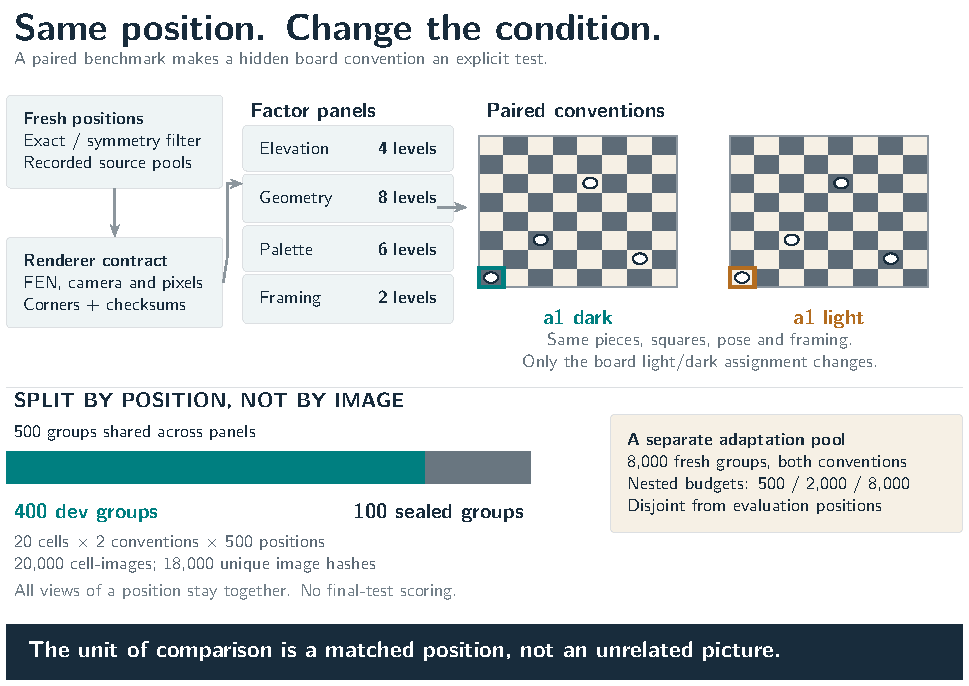
\includegraphics[width=\linewidth]{figures/generator.pdf}
\caption{Paired benchmark design. The boards are vector illustrations, not experimental frames. Each panel varies one factor; the convention is paired within every panel.}\label{fig:design}
\end{figure}

% Historical (v1) numbers below come from hash-pinned summary reports, not from original run
% receipts; see Appendix F for the provenance gap. v2 numbers come from receipts under paper/evidence/.
\section{Three ways the evaluation misled us}
\label{sec:lies}

Each subsection states what we believed, what the record shows, and the correct statement. The
three cases differ in kind. The first is a descriptive comparison between systems that differ in
more than one way. The second is a provenance failure. Only the third has a paired intervention
that isolates a cause. Numbers for the first two come from the earlier benchmark generation (v1:
18 splits, 5{,}800 frames, same generator lineage, a1-light convention throughout) and from public
real-photo sets. They are hash-pinned historical summaries, not original run receipts; Appendix~\ref{app:receipts}
records the gap. Numbers for the third come from the paired parity probes and from benchmark v2.
The probe, baseline and holdout-check result summaries are in the evidence index (Appendix~\ref{app:receipts}); per-image prediction files are not.

\subsection{A leaderboard-selected pipeline scores below its own member}
\label{sec:router}

The system we had shipped routed each image, by the detected board's apparent angle, to one of
three members: a full-frame recogniser initialised from ChessQueries (the \emph{raw member}) and
two recognisers that operate on a rectified board crop (the \emph{warp-high} and \emph{warp-low}
members). The router and its thresholds had been chosen on a private leaderboard. On our 18
controlled splits the shipped ensemble scores below its own raw member on 16, by up to 32.3
exact-board points on one piece family. The raw member alone reaches 100.0 on twelve splits
(Figure~\ref{fig:router}). Section~\ref{sec:cost} reports the latency of both systems.

Three further comparisons point the same way. Each carries a caveat that makes it a development
number, not a replication. SLCC test: 52.45 against 74.73, on 368 boards from 13 videos, and the
raw member had SLCC training data in its mix. CVChess: 1.42 against 98.86, on 352 photographs of
only 88 distinct positions. A held-out block of the training scenes: 99.30 against 100.00, on
held-out move blocks of the same games and scenes as training. On SLCC, above the routing
threshold the shipped ensemble drops the raw member and uses only the two warp members. Run alone
on all 368 boards, those members produce eight or more wrong squares on 234 and 236 boards. That
is consistent with failures in the detector and rectification stages on broadcast crops. We ran no
oracle-corner ablation on that cohort, so localisation and recognition failures are not separated.

Routing, member composition and training lineage all differ between the shipped ensemble and the
raw member, so this is not an isolated routing effect. We also have no intervention on leaderboard
exposure, so the reversal cannot be attributed to adaptive reuse rather than to distribution shift
between the leaderboard and these cohorts. What the record supports is this: a pipeline selected
% pooled v1: n-weighted over paper/evidence/reports/historical_pipeline.csv, 5,800 frames
on one private cohort scored below its own simpler member on the pooled v1 benchmark (91.8 against
98.5 exact over 5{,}800 frames) and on each of the three further cohorts. The two exceptions among
the 18 splits are the two lowest elevation bands, where the pipeline scores 88.8 against 88.6 and
98.0 against 97.0.

\subsection{Two holdouts contaminated by construction}
\label{sec:contamination}

An identifier-level leak check over the training mixes and every named holdout found that two
holdouts derived from ChessRender360 (1{,}635 and 1{,}263 images) shared image identifiers with
the mixes trained on them: 1{,}446 and 1{,}128 identifiers, 2{,}398 distinct, 2{,}574 counting both
sets (5{,}148 mix-by-identifier events over two mixes). Both holdouts were subsets of the same ten
thousand rectified images. The check reports
\texttt{clean: false}. The documented model-selection replay does not use those two holdouts, so
the recorded selection decisions were not influenced by them. That is not a proof that no earlier
or unrecorded decision was. A set can be named a holdout and still be training data. A check that
runs on identifiers and positions, not on directory names, is what caught it.

\subsection{A convention confound mistaken for a domain shift}
\label{sec:parity}

The ChessQueries release checkpoint produces zero exact boards on every one of the 18 v1 splits.
Its per-square accuracy of 52.7--56.7 is 4.6--9.0 points \emph{below} a constant all-empty
prediction, which also produces zero exact boards on these positions. The model places pieces on
the wrong squares; it does not default to empty. The same checkpoint through the same code path
scores 99.62 on ChessReD and 98.54 on ChessCog, which is also rendered. The failure appeared specific to
our rendering lineage. A crop diagnostic fed the checkpoint the first 150 boards of each of three
splits (450 in all) four ways: full frame, bounding-box crop, square-padded crop, and a perspective
warp to a square. None recovered an exact board under our convention, and per-square accuracy
moved by at most 1.2 points from full frame. At that point our own notes read ``the shift is the
piece and board appearance itself.''

It was not. Our renderer, following the convention of the data it had been matched to, makes a1 a
\emph{light} square. The laws of chess place a dark square at a1 \cite{fide}. Every public
chess-recognition source we could resolve follows that convention (Table~\ref{tab:conventions}).
The audit checks one representative image per source; the SLCC sample has no printed coordinates,
so its corner is recorded as unresolved. A preregistered paired probe changed exactly that one
renderer expression and nothing else, with byte-identical controls. On 192 positions in two
disjoint waves the checkpoint went from 0/192 to 18/192 exact ($+9.38$ points, 95\% paired bootstrap
$[5.73,13.54]$) and from 54.36 to 85.24 per-square ($+30.88$, $[28.91,32.76]$), removing 67.65\% of
wrong squares. Replicated on 288 positions across six other piece families,
the effect is 0/288 to 50/288 exact and 55.31 to 87.49 per-square. Swapping the model's learned
two-class query-colour indices \cite{chessqueries} in memory recovers 20.7 per-square points on a1-light images
but no exact board, and costs 2.9 points on a1-dark images. This is consistent with the colour
prior contributing to the failure; it does not isolate the mechanism. On the
development partition of benchmark v2 the release checkpoint scores 15.48 exact pooled under the
a1-dark convention, ranging from 0 to 34.25 across the twenty factor cells, and 0.0 in every cell
under a1-light (Figure~\ref{fig:heatmap}, left).
% receipt: evidence/tools/reports/paper/real_photo_2026-09-11/a1_light_2026-10-04/score_cq_cpu_20261004.json (a1_dark_armA, a1_light_primary)
One real-board check points the same way. The same ten positions were photographed on one physical
board with a dark a1, and on a later day, with a different phone and photographer, with a light a1.
The release checkpoint scores 76.25 and 57.97 per-square on the two sets of ten, with no exact
board in either, and the light arm scores lower on 8 of 10 positions. The arms differ in more than
parity, so this is a descriptive check, not a paired probe.

The corrected statement is about per-square accuracy. The convention accounts for about two thirds
of the wrong squares, and most boards still fail exactly after the correction (18/192 and 50/288).
On this cohort the residual is family-associated: two families stay at 0/48 exact while another
reaches 19/48. Positions differ between families here, so this describes the unchanged release
checkpoint; it is not a paired geometry effect, and it says nothing about what adaptation later
fixes. The paired geometry cells of v2 and the adaptation runs are the place to read those
(Section~\ref{sec:adaptation}). The trap had been written in our own research notes before the
benchmark was built, and we missed it anyway. Making the convention an explicit factor let it be
measured instead of inferred, which is why v2 carries it as its fifth axis.

A bounded follow-up on the same 192 positions found that, under the standard convention, a
ground-truth square crop raised exact boards from 18 to 27 while lowering per-square accuracy from
85.24 to 84.24. Framing is therefore not irrelevant once the convention is corrected. The
interaction is a trade-off measured on development positions with privileged localisation, not a
deployable improvement.

% historical source summary: evidence/reports/historical_pipeline.csv
\begin{figure}[htbp]
\centering
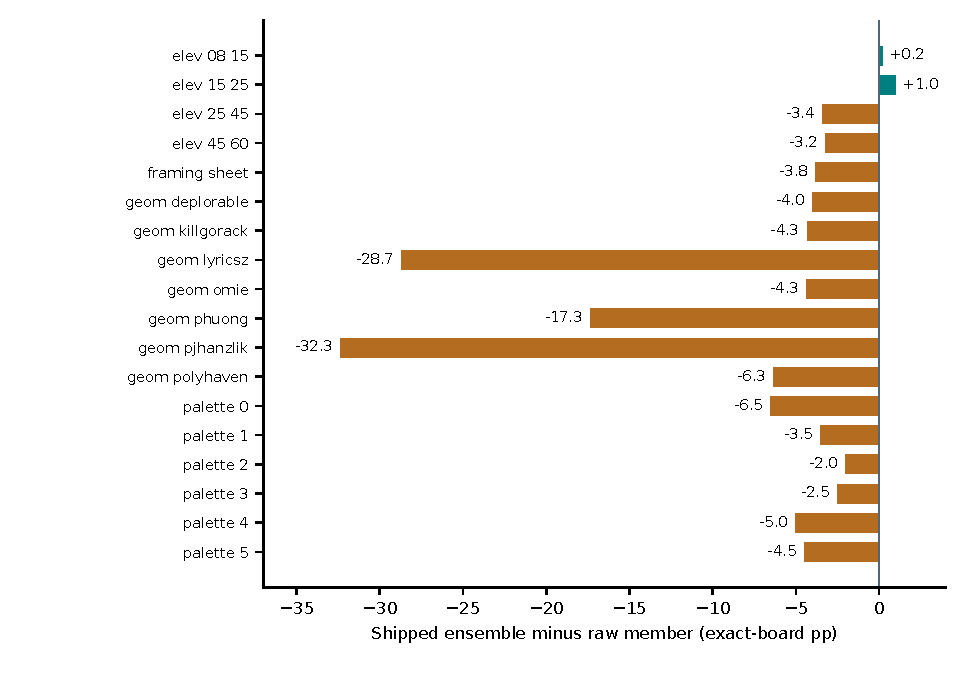
\includegraphics[width=\linewidth]{figures/router_harm.pdf}
\caption{Descriptive pipeline comparison on the earlier controlled splits. Member composition and routing both change; the difference is not an isolated routing effect. Historical aggregates are hash-pinned; original run-completion receipts are unavailable.}\label{fig:router}
\end{figure}

% receipt: evidence/tools/reports/paper/lora_curve_2026-09-10/lora_report.complete.json
\begin{figure}[htbp]
\centering
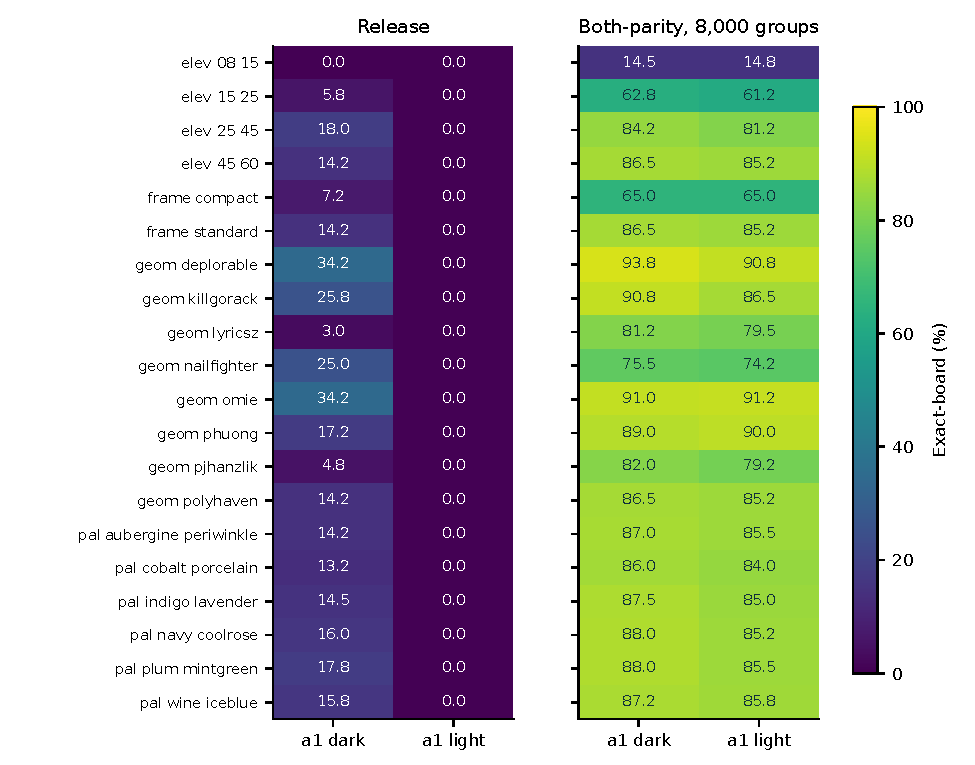
\includegraphics[width=\linewidth]{figures/heatmap.pdf}
\caption{Exact-board accuracy by development cell and convention. Left: released weights. Right: the largest both-convention adaptation run.}\label{fig:heatmap}
\end{figure}

\section{Matched-position adaptation and retention cost}
\label{sec:adaptation}

\subsection{Protocol}

% receipt: evidence/docs/LORA_CURVE_2026-09-10.md
We adapt only the encoder with the upstream low-rank modules~\citep{lora,chessqueries}. The registered
configuration uses rank 8, alpha 16, dropout 0.05, AdamW at a learning rate of
$10^{-4}$ with zero weight decay, no scheduler, and no warm-up. The base
encoder and the complete readout remain frozen. Every run uses batch size 6,
bf16 autocast, and exactly 1,500 optimizer updates, with no image augmentation,
early stopping, or development-selected checkpoint.

% receipt: evidence/benchmark_v2/adaptation.complete.json
% receipt: evidence/docs/ADAPTATION_POOL_2026-09-10.md; Scene sampling and nested budgets
Training uses a separate pool of 8,000 fresh position groups, each rendered at
both board conventions. The 500-, 2,000-, and 8,000-group budgets are nested
prefixes of one fixed permutation. The dark-only and both-convention arms use
the same positions and the same number of optimizer updates, but not the same
number of distinct images: a both-convention pool contains twice as many
available views. Unlike the evaluation panels, adaptation examples combine factor
levels with balanced marginals. The pool includes the reference material scheme
as well as the palette treatments; matching the supported levels does not make
the joint training and evaluation scene distributions identical.

% receipt: evidence/docs/records/C2_BUDGET_SEMANTICS_2026-09-10.md
Each run makes 9,000 image presentations. Thus the largest both-convention pool
cannot be covered in full under the fixed step cap. The budget denotes available
position groups, not measured unique examples seen or complete epochs. The
experiments compare matched positions and fixed optimizer exposure rather than
equal distinct-image counts.

% receipt: evidence/tools/reports/paper/lora_curve_2026-09-10/lora_report.json
All checkpoints are evaluated on the same 16,000 development cell-images from
400 position groups. The separate photo retention set contains 2,129 boards;
the preregistered pass threshold is 99.12\% exact-board accuracy. The sealed
final test is not evaluated. The middle budget uses three fixed training seeds,
while the other budgets use one, and every registered result is retained.

\subsection{Adaptation curve}

% receipt: evidence/tools/reports/paper/lora_curve_2026-09-10/lora_report.json
The release checkpoint begins at 15.48\% exact accuracy on a1-dark development
cells and 0.00\% on a1-light cells. Dark-only adaptation raises a1-dark accuracy
to 64.70\% with 500 groups and 79.70\% with 8,000 groups, but a1-light exact
accuracy remains 0.00\% at every dark-only budget. At 8,000 groups, the
both-convention arm reaches 80.65\% on a1-dark cells and 79.03\% on a1-light
cells. Figure~\ref{fig:adaptation} shows all seeds and budgets; the full numeric
matrix appears in Table~\ref{tab:adaptation}.

\begingroup\small
\setlength{\tabcolsep}{4pt}
\begin{table}[htbp]\centering
\caption{All fixed-step runs. Synthetic cells are paired; photo counts use the same retention set.}\label{tab:adaptation}
\begin{tabular}{lrrrrr}
\toprule
Run & % receipt: evidence/tools/reports/paper/lora_curve_2026-09-10/lora_report.complete.json; source: evidence/tools/reports/paper/lora_curve_2026-09-10/lora_report.json; column definitions
Dark (\%) & % receipt: evidence/tools/reports/paper/lora_curve_2026-09-10/lora_report.complete.json; source: evidence/tools/reports/paper/lora_curve_2026-09-10/lora_report.json; column definitions
Light (\%) & % receipt: evidence/tools/reports/paper/lora_curve_2026-09-10/lora_report.complete.json; source: evidence/tools/reports/paper/lora_curve_2026-09-10/lora_report.json; column definitions
Photo (\%) & % receipt: evidence/tools/reports/paper/lora_curve_2026-09-10/lora_report.complete.json; source: evidence/tools/reports/paper/lora_curve_2026-09-10/lora_report.json; column definitions
Photo exact & % receipt: evidence/tools/reports/paper/lora_curve_2026-09-10/lora_report.complete.json; source: evidence/tools/reports/paper/lora_curve_2026-09-10/lora_report.json; column definitions
Gate \\ % receipt: evidence/tools/reports/paper/lora_curve_2026-09-10/lora_report.complete.json; source: evidence/tools/reports/paper/lora_curve_2026-09-10/lora_report.json; column definitions
\midrule

release & % receipt: evidence/tools/reports/paper/lora_curve_2026-09-10/lora_report.complete.json; source: evidence/tools/reports/paper/lora_curve_2026-09-10/lora_report.json; release/metrics
15.48 & % receipt: evidence/tools/reports/paper/lora_curve_2026-09-10/lora_report.complete.json; source: evidence/tools/reports/paper/lora_curve_2026-09-10/lora_report.json; release/metrics
0.00 & % receipt: evidence/tools/reports/paper/lora_curve_2026-09-10/lora_report.complete.json; source: evidence/tools/reports/paper/lora_curve_2026-09-10/lora_report.json; release/metrics
99.62 & % receipt: evidence/tools/reports/paper/lora_curve_2026-09-10/lora_report.complete.json; source: evidence/tools/reports/paper/lora_curve_2026-09-10/lora_report.json; release/metrics
2121 & % receipt: evidence/tools/reports/paper/lora_curve_2026-09-10/lora_report.complete.json; source: evidence/tools/reports/paper/lora_curve_2026-09-10/lora_report.json; release/metrics
reference \\ % receipt: evidence/tools/reports/paper/lora_curve_2026-09-10/lora_report.complete.json; source: evidence/tools/reports/paper/lora_curve_2026-09-10/lora_report.json; release/metrics

b500\_\allowbreak{}dark\_\allowbreak{}s303 & % receipt: evidence/tools/reports/paper/lora_curve_2026-09-10/lora_report.complete.json; source: evidence/tools/reports/paper/lora_curve_2026-09-10/lora_report.json; b500_dark_s303/metrics
64.70 & % receipt: evidence/tools/reports/paper/lora_curve_2026-09-10/lora_report.complete.json; source: evidence/tools/reports/paper/lora_curve_2026-09-10/lora_report.json; b500_dark_s303/metrics
0.00 & % receipt: evidence/tools/reports/paper/lora_curve_2026-09-10/lora_report.complete.json; source: evidence/tools/reports/paper/lora_curve_2026-09-10/lora_report.json; b500_dark_s303/metrics
99.11 & % receipt: evidence/tools/reports/paper/lora_curve_2026-09-10/lora_report.complete.json; source: evidence/tools/reports/paper/lora_curve_2026-09-10/lora_report.json; b500_dark_s303/metrics
2110 & % receipt: evidence/tools/reports/paper/lora_curve_2026-09-10/lora_report.complete.json; source: evidence/tools/reports/paper/lora_curve_2026-09-10/lora_report.json; b500_dark_s303/metrics
fail \\ % receipt: evidence/tools/reports/paper/lora_curve_2026-09-10/lora_report.complete.json; source: evidence/tools/reports/paper/lora_curve_2026-09-10/lora_report.json; b500_dark_s303/metrics

b500\_\allowbreak{}both\_\allowbreak{}s303 & % receipt: evidence/tools/reports/paper/lora_curve_2026-09-10/lora_report.complete.json; source: evidence/tools/reports/paper/lora_curve_2026-09-10/lora_report.json; b500_both_s303/metrics
66.80 & % receipt: evidence/tools/reports/paper/lora_curve_2026-09-10/lora_report.complete.json; source: evidence/tools/reports/paper/lora_curve_2026-09-10/lora_report.json; b500_both_s303/metrics
64.20 & % receipt: evidence/tools/reports/paper/lora_curve_2026-09-10/lora_report.complete.json; source: evidence/tools/reports/paper/lora_curve_2026-09-10/lora_report.json; b500_both_s303/metrics
99.01 & % receipt: evidence/tools/reports/paper/lora_curve_2026-09-10/lora_report.complete.json; source: evidence/tools/reports/paper/lora_curve_2026-09-10/lora_report.json; b500_both_s303/metrics
2108 & % receipt: evidence/tools/reports/paper/lora_curve_2026-09-10/lora_report.complete.json; source: evidence/tools/reports/paper/lora_curve_2026-09-10/lora_report.json; b500_both_s303/metrics
fail \\ % receipt: evidence/tools/reports/paper/lora_curve_2026-09-10/lora_report.complete.json; source: evidence/tools/reports/paper/lora_curve_2026-09-10/lora_report.json; b500_both_s303/metrics

b2000\_\allowbreak{}dark\_\allowbreak{}s303 & % receipt: evidence/tools/reports/paper/lora_curve_2026-09-10/lora_report.complete.json; source: evidence/tools/reports/paper/lora_curve_2026-09-10/lora_report.json; b2000_dark_s303/metrics
77.85 & % receipt: evidence/tools/reports/paper/lora_curve_2026-09-10/lora_report.complete.json; source: evidence/tools/reports/paper/lora_curve_2026-09-10/lora_report.json; b2000_dark_s303/metrics
0.00 & % receipt: evidence/tools/reports/paper/lora_curve_2026-09-10/lora_report.complete.json; source: evidence/tools/reports/paper/lora_curve_2026-09-10/lora_report.json; b2000_dark_s303/metrics
99.01 & % receipt: evidence/tools/reports/paper/lora_curve_2026-09-10/lora_report.complete.json; source: evidence/tools/reports/paper/lora_curve_2026-09-10/lora_report.json; b2000_dark_s303/metrics
2108 & % receipt: evidence/tools/reports/paper/lora_curve_2026-09-10/lora_report.complete.json; source: evidence/tools/reports/paper/lora_curve_2026-09-10/lora_report.json; b2000_dark_s303/metrics
fail \\ % receipt: evidence/tools/reports/paper/lora_curve_2026-09-10/lora_report.complete.json; source: evidence/tools/reports/paper/lora_curve_2026-09-10/lora_report.json; b2000_dark_s303/metrics

b2000\_\allowbreak{}both\_\allowbreak{}s303 & % receipt: evidence/tools/reports/paper/lora_curve_2026-09-10/lora_report.complete.json; source: evidence/tools/reports/paper/lora_curve_2026-09-10/lora_report.json; b2000_both_s303/metrics
74.24 & % receipt: evidence/tools/reports/paper/lora_curve_2026-09-10/lora_report.complete.json; source: evidence/tools/reports/paper/lora_curve_2026-09-10/lora_report.json; b2000_both_s303/metrics
71.99 & % receipt: evidence/tools/reports/paper/lora_curve_2026-09-10/lora_report.complete.json; source: evidence/tools/reports/paper/lora_curve_2026-09-10/lora_report.json; b2000_both_s303/metrics
98.54 & % receipt: evidence/tools/reports/paper/lora_curve_2026-09-10/lora_report.complete.json; source: evidence/tools/reports/paper/lora_curve_2026-09-10/lora_report.json; b2000_both_s303/metrics
2098 & % receipt: evidence/tools/reports/paper/lora_curve_2026-09-10/lora_report.complete.json; source: evidence/tools/reports/paper/lora_curve_2026-09-10/lora_report.json; b2000_both_s303/metrics
fail \\ % receipt: evidence/tools/reports/paper/lora_curve_2026-09-10/lora_report.complete.json; source: evidence/tools/reports/paper/lora_curve_2026-09-10/lora_report.json; b2000_both_s303/metrics

b2000\_\allowbreak{}dark\_\allowbreak{}s304 & % receipt: evidence/tools/reports/paper/lora_curve_2026-09-10/lora_report.complete.json; source: evidence/tools/reports/paper/lora_curve_2026-09-10/lora_report.json; b2000_dark_s304/metrics
76.83 & % receipt: evidence/tools/reports/paper/lora_curve_2026-09-10/lora_report.complete.json; source: evidence/tools/reports/paper/lora_curve_2026-09-10/lora_report.json; b2000_dark_s304/metrics
0.00 & % receipt: evidence/tools/reports/paper/lora_curve_2026-09-10/lora_report.complete.json; source: evidence/tools/reports/paper/lora_curve_2026-09-10/lora_report.json; b2000_dark_s304/metrics
99.06 & % receipt: evidence/tools/reports/paper/lora_curve_2026-09-10/lora_report.complete.json; source: evidence/tools/reports/paper/lora_curve_2026-09-10/lora_report.json; b2000_dark_s304/metrics
2109 & % receipt: evidence/tools/reports/paper/lora_curve_2026-09-10/lora_report.complete.json; source: evidence/tools/reports/paper/lora_curve_2026-09-10/lora_report.json; b2000_dark_s304/metrics
fail \\ % receipt: evidence/tools/reports/paper/lora_curve_2026-09-10/lora_report.complete.json; source: evidence/tools/reports/paper/lora_curve_2026-09-10/lora_report.json; b2000_dark_s304/metrics

b2000\_\allowbreak{}both\_\allowbreak{}s304 & % receipt: evidence/tools/reports/paper/lora_curve_2026-09-10/lora_report.complete.json; source: evidence/tools/reports/paper/lora_curve_2026-09-10/lora_report.json; b2000_both_s304/metrics
73.64 & % receipt: evidence/tools/reports/paper/lora_curve_2026-09-10/lora_report.complete.json; source: evidence/tools/reports/paper/lora_curve_2026-09-10/lora_report.json; b2000_both_s304/metrics
72.24 & % receipt: evidence/tools/reports/paper/lora_curve_2026-09-10/lora_report.complete.json; source: evidence/tools/reports/paper/lora_curve_2026-09-10/lora_report.json; b2000_both_s304/metrics
98.92 & % receipt: evidence/tools/reports/paper/lora_curve_2026-09-10/lora_report.complete.json; source: evidence/tools/reports/paper/lora_curve_2026-09-10/lora_report.json; b2000_both_s304/metrics
2106 & % receipt: evidence/tools/reports/paper/lora_curve_2026-09-10/lora_report.complete.json; source: evidence/tools/reports/paper/lora_curve_2026-09-10/lora_report.json; b2000_both_s304/metrics
fail \\ % receipt: evidence/tools/reports/paper/lora_curve_2026-09-10/lora_report.complete.json; source: evidence/tools/reports/paper/lora_curve_2026-09-10/lora_report.json; b2000_both_s304/metrics

b2000\_\allowbreak{}dark\_\allowbreak{}s305 & % receipt: evidence/tools/reports/paper/lora_curve_2026-09-10/lora_report.complete.json; source: evidence/tools/reports/paper/lora_curve_2026-09-10/lora_report.json; b2000_dark_s305/metrics
77.80 & % receipt: evidence/tools/reports/paper/lora_curve_2026-09-10/lora_report.complete.json; source: evidence/tools/reports/paper/lora_curve_2026-09-10/lora_report.json; b2000_dark_s305/metrics
0.00 & % receipt: evidence/tools/reports/paper/lora_curve_2026-09-10/lora_report.complete.json; source: evidence/tools/reports/paper/lora_curve_2026-09-10/lora_report.json; b2000_dark_s305/metrics
98.97 & % receipt: evidence/tools/reports/paper/lora_curve_2026-09-10/lora_report.complete.json; source: evidence/tools/reports/paper/lora_curve_2026-09-10/lora_report.json; b2000_dark_s305/metrics
2107 & % receipt: evidence/tools/reports/paper/lora_curve_2026-09-10/lora_report.complete.json; source: evidence/tools/reports/paper/lora_curve_2026-09-10/lora_report.json; b2000_dark_s305/metrics
fail \\ % receipt: evidence/tools/reports/paper/lora_curve_2026-09-10/lora_report.complete.json; source: evidence/tools/reports/paper/lora_curve_2026-09-10/lora_report.json; b2000_dark_s305/metrics

b2000\_\allowbreak{}both\_\allowbreak{}s305 & % receipt: evidence/tools/reports/paper/lora_curve_2026-09-10/lora_report.complete.json; source: evidence/tools/reports/paper/lora_curve_2026-09-10/lora_report.json; b2000_both_s305/metrics
76.63 & % receipt: evidence/tools/reports/paper/lora_curve_2026-09-10/lora_report.complete.json; source: evidence/tools/reports/paper/lora_curve_2026-09-10/lora_report.json; b2000_both_s305/metrics
75.90 & % receipt: evidence/tools/reports/paper/lora_curve_2026-09-10/lora_report.complete.json; source: evidence/tools/reports/paper/lora_curve_2026-09-10/lora_report.json; b2000_both_s305/metrics
98.59 & % receipt: evidence/tools/reports/paper/lora_curve_2026-09-10/lora_report.complete.json; source: evidence/tools/reports/paper/lora_curve_2026-09-10/lora_report.json; b2000_both_s305/metrics
2099 & % receipt: evidence/tools/reports/paper/lora_curve_2026-09-10/lora_report.complete.json; source: evidence/tools/reports/paper/lora_curve_2026-09-10/lora_report.json; b2000_both_s305/metrics
fail \\ % receipt: evidence/tools/reports/paper/lora_curve_2026-09-10/lora_report.complete.json; source: evidence/tools/reports/paper/lora_curve_2026-09-10/lora_report.json; b2000_both_s305/metrics

b8000\_\allowbreak{}dark\_\allowbreak{}s303 & % receipt: evidence/tools/reports/paper/lora_curve_2026-09-10/lora_report.complete.json; source: evidence/tools/reports/paper/lora_curve_2026-09-10/lora_report.json; b8000_dark_s303/metrics
79.70 & % receipt: evidence/tools/reports/paper/lora_curve_2026-09-10/lora_report.complete.json; source: evidence/tools/reports/paper/lora_curve_2026-09-10/lora_report.json; b8000_dark_s303/metrics
0.00 & % receipt: evidence/tools/reports/paper/lora_curve_2026-09-10/lora_report.complete.json; source: evidence/tools/reports/paper/lora_curve_2026-09-10/lora_report.json; b8000_dark_s303/metrics
99.11 & % receipt: evidence/tools/reports/paper/lora_curve_2026-09-10/lora_report.complete.json; source: evidence/tools/reports/paper/lora_curve_2026-09-10/lora_report.json; b8000_dark_s303/metrics
2110 & % receipt: evidence/tools/reports/paper/lora_curve_2026-09-10/lora_report.complete.json; source: evidence/tools/reports/paper/lora_curve_2026-09-10/lora_report.json; b8000_dark_s303/metrics
fail \\ % receipt: evidence/tools/reports/paper/lora_curve_2026-09-10/lora_report.complete.json; source: evidence/tools/reports/paper/lora_curve_2026-09-10/lora_report.json; b8000_dark_s303/metrics

b8000\_\allowbreak{}both\_\allowbreak{}s303 & % receipt: evidence/tools/reports/paper/lora_curve_2026-09-10/lora_report.complete.json; source: evidence/tools/reports/paper/lora_curve_2026-09-10/lora_report.json; b8000_both_s303/metrics
80.65 & % receipt: evidence/tools/reports/paper/lora_curve_2026-09-10/lora_report.complete.json; source: evidence/tools/reports/paper/lora_curve_2026-09-10/lora_report.json; b8000_both_s303/metrics
79.03 & % receipt: evidence/tools/reports/paper/lora_curve_2026-09-10/lora_report.complete.json; source: evidence/tools/reports/paper/lora_curve_2026-09-10/lora_report.json; b8000_both_s303/metrics
98.59 & % receipt: evidence/tools/reports/paper/lora_curve_2026-09-10/lora_report.complete.json; source: evidence/tools/reports/paper/lora_curve_2026-09-10/lora_report.json; b8000_both_s303/metrics
2099 & % receipt: evidence/tools/reports/paper/lora_curve_2026-09-10/lora_report.complete.json; source: evidence/tools/reports/paper/lora_curve_2026-09-10/lora_report.json; b8000_both_s303/metrics
fail \\ % receipt: evidence/tools/reports/paper/lora_curve_2026-09-10/lora_report.complete.json; source: evidence/tools/reports/paper/lora_curve_2026-09-10/lora_report.json; b8000_both_s303/metrics

\bottomrule
\end{tabular}
\end{table}
\endgroup


% receipt: evidence/tools/reports/paper/lora_curve_2026-09-10/lora_report.json; metrics/dev/by_parity
The standard-convention difference between arms depends on budget. Both-convention
minus dark-only accuracy is $+2.10$ points at 500 groups, $-2.66$ points for the
three-seed mean at 2,000 groups, and $+0.95$ points at 8,000 groups. There is no
budget-independent standard-convention penalty. These are point estimates, not
paired between-arm confidence intervals.

% receipt: evidence/tools/reports/paper/lora_curve_2026-09-10/lora_report.json; b8000_both_s303/metrics/paired_vs_release
As one measure of position-sampling uncertainty, the largest both-convention run
improves the cell-weighted score pooled over both conventions by 72.10 points
relative to release, with a stored 95\% group-bootstrap interval of
$[69.90,74.21]$. This is not an interval for the arm contrast or for unseen real
photographs. The machine-readable report retains each run's pooled and per-cell
intervals and gained/lost counts; the tables print point estimates.

% receipt: evidence/tools/reports/paper/lora_curve_2026-09-10/lora_report.json
No adapted checkpoint passes the registered photo-retention gate. Across the
ten runs, exact accuracy on that set falls from the 99.62\% release reference to
between 98.54\% and 99.11\%. This corresponds to 11--23 additional incorrect
boards. These are net changes in exact-board counts on the same photo set, not
counts of all previously correct boards that became incorrect. The loss is not
monotone in synthetic data budget; these measurements do not identify its cause.

% receipt: evidence/tools/reports/paper/lora_curve_2026-09-10/lora_report.json
Recovery is not uniform across the measured cells. Under the
largest both-convention run, the lowest-elevation a1-dark cell reaches only
14.50\% exact accuracy while the reference-elevation cell reaches 86.50\%.
Geometry effects also remain visible. Figure~\ref{fig:heatmap} reports all
factor cells for the release checkpoint and the largest both-convention run.

\subsection{Reading the intervention}

The experiments support three bounded conclusions. First, much of the release
checkpoint's synthetic gap is reducible with matched rendered data. Second,
the one-sided runs produce no exact boards under the other convention in this
protocol; that does not imply zero per-square learning.
Third, adding the convention mate is sufficient to remove most of that asymmetry,
but it does not satisfy the real-photo retention criterion and does not resolve
low-elevation error. These are development results for one architecture and one
fixed adapter recipe, not evidence of general robustness.

\subsection{Residual error characterization}

% receipt: evidence/tools/reports/paper/residual_shift_2026-09-10/r1/residual_r1.metrics.json
A separate preregistered diagnostic examines 288 canonical a1-dark boards from
six geometry families using the unchanged release checkpoint, not a LoRA-adapted model. The families
use different positions, so their comparison does not isolate geometry. Lyricsz and
PJ~Hanzlik each have 0 exact boards among 48. For these families, binary
presence errors account for 66.86\% and 73.71\% of wrong squares, respectively;
the remainder are wrong occupied classes. This decomposition describes the
failure but does not establish its cause.

% receipt: evidence/tools/reports/paper/residual_shift_2026-09-10/r1/residual_r1.complete.json
% receipt: evidence/docs/C3_PRECISION_AMENDMENT_2026-09-10.md
The accompanying attention sample was chosen without reference to prediction
outcomes and retains all 64 final-decoder query maps for 30 boards. The maps use
head averages and per-query display normalization. Appendix~\ref{app:attention}
shows fixed examples. The capture used the preregistered precision amendment after
an initial forward-equivalence failure; its numerical checks were passed before
interpretation. Attention is treated only as descriptive localization
evidence; no attention intervention or mechanism test was performed.
% receipt: evidence/tools/reports/paper/lora_curve_2026-09-10/lora_report.complete.json
\begin{figure}[htbp]
\centering
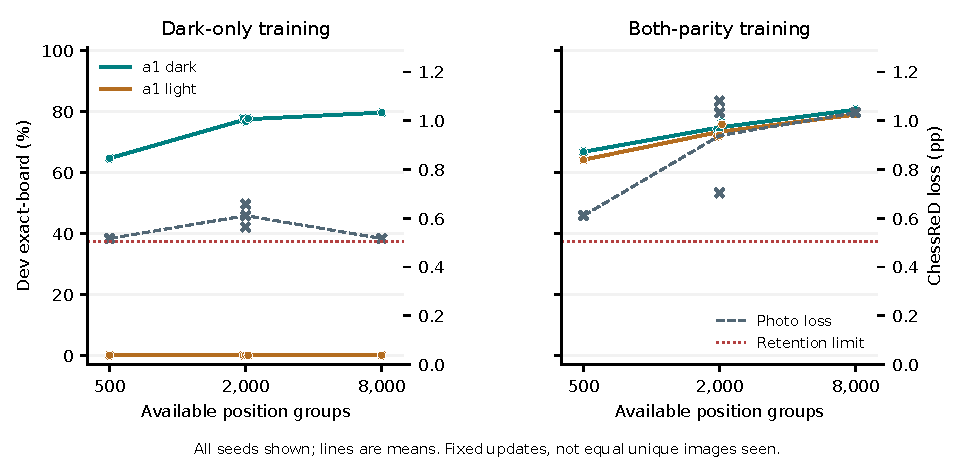
\includegraphics[width=\linewidth]{figures/adaptation.pdf}
\caption{Fixed-step adaptation. Points show all seeds; lines join budget-wise means. The right axis measures loss on the same real-photo retention set.}\label{fig:adaptation}
\end{figure}

\section{Inference cost}
\label{sec:cost}

% receipt: evidence/tools/reports/paper/timing_2026-09-10/timing.runs/cq_release.complete.json
We measure synchronized native-inference latency on an NVIDIA RTX 3090,
with no competing GPU compute process detected, at a fixed 270~W power limit. A fixed development subset supplies 500 images
from 250 factor-cell scenes. Each system runs in
a fresh process with batch size 1 and native FP16 autocast. The harness excludes
file decode and 30 warm-up images, while retaining resize, normalization,
device transfer, model execution, routing, warping, test-time augmentation, host
transfer, and notation construction whenever the native pipeline uses them.

% receipt: evidence/tools/reports/paper/timing_2026-09-10/timing.runs.json
The release checkpoint has median latency 64.41~ms per image. The raw member
requires 79.69~ms, while the shipped ensemble requires 195.52~ms. The ten
adapted checkpoints lie between 71.50 and 73.12~ms, so their measured median
overhead relative to the release checkpoint is 7.09--8.71~ms in this harness.
Table~\ref{tab:timing} reports medians and ninetieth percentiles for every
system, and Figure~\ref{fig:timing} visualizes the same receipt-bound values.

\begingroup\small
\setlength{\tabcolsep}{4pt}
\begin{table}[htbp]\centering
\caption{Synchronized single-image latency on the same isolated device.}\label{tab:timing}
\begin{tabular}{lrrr}
\toprule
System & % receipt: evidence/tools/reports/paper/timing_2026-09-10/timing.complete.json; source: evidence/tools/reports/paper/timing_2026-09-10/timing.runs.json; column definitions
Images & % receipt: evidence/tools/reports/paper/timing_2026-09-10/timing.complete.json; source: evidence/tools/reports/paper/timing_2026-09-10/timing.runs.json; column definitions
Median (ms) & % receipt: evidence/tools/reports/paper/timing_2026-09-10/timing.complete.json; source: evidence/tools/reports/paper/timing_2026-09-10/timing.runs.json; column definitions
P90 (ms) \\ % receipt: evidence/tools/reports/paper/timing_2026-09-10/timing.complete.json; source: evidence/tools/reports/paper/timing_2026-09-10/timing.runs.json; column definitions
\midrule

ChessQueries release & % receipt: evidence/tools/reports/paper/timing_2026-09-10/timing.complete.json; source: evidence/tools/reports/paper/timing_2026-09-10/timing.runs.json; cq_release/summary
500 & % receipt: evidence/tools/reports/paper/timing_2026-09-10/timing.complete.json; source: evidence/tools/reports/paper/timing_2026-09-10/timing.runs.json; cq_release/summary
64.41 & % receipt: evidence/tools/reports/paper/timing_2026-09-10/timing.complete.json; source: evidence/tools/reports/paper/timing_2026-09-10/timing.runs.json; cq_release/summary
65.72 \\ % receipt: evidence/tools/reports/paper/timing_2026-09-10/timing.complete.json; source: evidence/tools/reports/paper/timing_2026-09-10/timing.runs.json; cq_release/summary

shipped ensemble & % receipt: evidence/tools/reports/paper/timing_2026-09-10/timing.complete.json; source: evidence/tools/reports/paper/timing_2026-09-10/timing.runs.json; private_full/summary
500 & % receipt: evidence/tools/reports/paper/timing_2026-09-10/timing.complete.json; source: evidence/tools/reports/paper/timing_2026-09-10/timing.runs.json; private_full/summary
195.52 & % receipt: evidence/tools/reports/paper/timing_2026-09-10/timing.complete.json; source: evidence/tools/reports/paper/timing_2026-09-10/timing.runs.json; private_full/summary
244.22 \\ % receipt: evidence/tools/reports/paper/timing_2026-09-10/timing.complete.json; source: evidence/tools/reports/paper/timing_2026-09-10/timing.runs.json; private_full/summary

raw member & % receipt: evidence/tools/reports/paper/timing_2026-09-10/timing.complete.json; source: evidence/tools/reports/paper/timing_2026-09-10/timing.runs.json; private_raw/summary
500 & % receipt: evidence/tools/reports/paper/timing_2026-09-10/timing.complete.json; source: evidence/tools/reports/paper/timing_2026-09-10/timing.runs.json; private_raw/summary
79.69 & % receipt: evidence/tools/reports/paper/timing_2026-09-10/timing.complete.json; source: evidence/tools/reports/paper/timing_2026-09-10/timing.runs.json; private_raw/summary
81.07 \\ % receipt: evidence/tools/reports/paper/timing_2026-09-10/timing.complete.json; source: evidence/tools/reports/paper/timing_2026-09-10/timing.runs.json; private_raw/summary

warp-high member & % receipt: evidence/tools/reports/paper/timing_2026-09-10/timing.complete.json; source: evidence/tools/reports/paper/timing_2026-09-10/timing.runs.json; private_warp_high/summary
500 & % receipt: evidence/tools/reports/paper/timing_2026-09-10/timing.complete.json; source: evidence/tools/reports/paper/timing_2026-09-10/timing.runs.json; private_warp_high/summary
195.23 & % receipt: evidence/tools/reports/paper/timing_2026-09-10/timing.complete.json; source: evidence/tools/reports/paper/timing_2026-09-10/timing.runs.json; private_warp_high/summary
197.55 \\ % receipt: evidence/tools/reports/paper/timing_2026-09-10/timing.complete.json; source: evidence/tools/reports/paper/timing_2026-09-10/timing.runs.json; private_warp_high/summary

warp-low member & % receipt: evidence/tools/reports/paper/timing_2026-09-10/timing.complete.json; source: evidence/tools/reports/paper/timing_2026-09-10/timing.runs.json; private_warp_low/summary
500 & % receipt: evidence/tools/reports/paper/timing_2026-09-10/timing.complete.json; source: evidence/tools/reports/paper/timing_2026-09-10/timing.runs.json; private_warp_low/summary
168.98 & % receipt: evidence/tools/reports/paper/timing_2026-09-10/timing.complete.json; source: evidence/tools/reports/paper/timing_2026-09-10/timing.runs.json; private_warp_low/summary
170.85 \\ % receipt: evidence/tools/reports/paper/timing_2026-09-10/timing.complete.json; source: evidence/tools/reports/paper/timing_2026-09-10/timing.runs.json; private_warp_low/summary

LoRA dark n500 s303 & % receipt: evidence/tools/reports/paper/timing_2026-09-10/timing.complete.json; source: evidence/tools/reports/paper/timing_2026-09-10/timing.runs.json; lora_dark_n500_s303/summary
500 & % receipt: evidence/tools/reports/paper/timing_2026-09-10/timing.complete.json; source: evidence/tools/reports/paper/timing_2026-09-10/timing.runs.json; lora_dark_n500_s303/summary
71.88 & % receipt: evidence/tools/reports/paper/timing_2026-09-10/timing.complete.json; source: evidence/tools/reports/paper/timing_2026-09-10/timing.runs.json; lora_dark_n500_s303/summary
72.64 \\ % receipt: evidence/tools/reports/paper/timing_2026-09-10/timing.complete.json; source: evidence/tools/reports/paper/timing_2026-09-10/timing.runs.json; lora_dark_n500_s303/summary

LoRA both n500 s303 & % receipt: evidence/tools/reports/paper/timing_2026-09-10/timing.complete.json; source: evidence/tools/reports/paper/timing_2026-09-10/timing.runs.json; lora_both_n500_s303/summary
500 & % receipt: evidence/tools/reports/paper/timing_2026-09-10/timing.complete.json; source: evidence/tools/reports/paper/timing_2026-09-10/timing.runs.json; lora_both_n500_s303/summary
72.40 & % receipt: evidence/tools/reports/paper/timing_2026-09-10/timing.complete.json; source: evidence/tools/reports/paper/timing_2026-09-10/timing.runs.json; lora_both_n500_s303/summary
73.32 \\ % receipt: evidence/tools/reports/paper/timing_2026-09-10/timing.complete.json; source: evidence/tools/reports/paper/timing_2026-09-10/timing.runs.json; lora_both_n500_s303/summary

LoRA dark n2000 s303 & % receipt: evidence/tools/reports/paper/timing_2026-09-10/timing.complete.json; source: evidence/tools/reports/paper/timing_2026-09-10/timing.runs.json; lora_dark_n2000_s303/summary
500 & % receipt: evidence/tools/reports/paper/timing_2026-09-10/timing.complete.json; source: evidence/tools/reports/paper/timing_2026-09-10/timing.runs.json; lora_dark_n2000_s303/summary
72.29 & % receipt: evidence/tools/reports/paper/timing_2026-09-10/timing.complete.json; source: evidence/tools/reports/paper/timing_2026-09-10/timing.runs.json; lora_dark_n2000_s303/summary
73.08 \\ % receipt: evidence/tools/reports/paper/timing_2026-09-10/timing.complete.json; source: evidence/tools/reports/paper/timing_2026-09-10/timing.runs.json; lora_dark_n2000_s303/summary

LoRA both n2000 s303 & % receipt: evidence/tools/reports/paper/timing_2026-09-10/timing.complete.json; source: evidence/tools/reports/paper/timing_2026-09-10/timing.runs.json; lora_both_n2000_s303/summary
500 & % receipt: evidence/tools/reports/paper/timing_2026-09-10/timing.complete.json; source: evidence/tools/reports/paper/timing_2026-09-10/timing.runs.json; lora_both_n2000_s303/summary
71.50 & % receipt: evidence/tools/reports/paper/timing_2026-09-10/timing.complete.json; source: evidence/tools/reports/paper/timing_2026-09-10/timing.runs.json; lora_both_n2000_s303/summary
72.50 \\ % receipt: evidence/tools/reports/paper/timing_2026-09-10/timing.complete.json; source: evidence/tools/reports/paper/timing_2026-09-10/timing.runs.json; lora_both_n2000_s303/summary

LoRA dark n2000 s304 & % receipt: evidence/tools/reports/paper/timing_2026-09-10/timing.complete.json; source: evidence/tools/reports/paper/timing_2026-09-10/timing.runs.json; lora_dark_n2000_s304/summary
500 & % receipt: evidence/tools/reports/paper/timing_2026-09-10/timing.complete.json; source: evidence/tools/reports/paper/timing_2026-09-10/timing.runs.json; lora_dark_n2000_s304/summary
71.86 & % receipt: evidence/tools/reports/paper/timing_2026-09-10/timing.complete.json; source: evidence/tools/reports/paper/timing_2026-09-10/timing.runs.json; lora_dark_n2000_s304/summary
72.95 \\ % receipt: evidence/tools/reports/paper/timing_2026-09-10/timing.complete.json; source: evidence/tools/reports/paper/timing_2026-09-10/timing.runs.json; lora_dark_n2000_s304/summary

LoRA both n2000 s304 & % receipt: evidence/tools/reports/paper/timing_2026-09-10/timing.complete.json; source: evidence/tools/reports/paper/timing_2026-09-10/timing.runs.json; lora_both_n2000_s304/summary
500 & % receipt: evidence/tools/reports/paper/timing_2026-09-10/timing.complete.json; source: evidence/tools/reports/paper/timing_2026-09-10/timing.runs.json; lora_both_n2000_s304/summary
72.80 & % receipt: evidence/tools/reports/paper/timing_2026-09-10/timing.complete.json; source: evidence/tools/reports/paper/timing_2026-09-10/timing.runs.json; lora_both_n2000_s304/summary
73.68 \\ % receipt: evidence/tools/reports/paper/timing_2026-09-10/timing.complete.json; source: evidence/tools/reports/paper/timing_2026-09-10/timing.runs.json; lora_both_n2000_s304/summary

LoRA dark n2000 s305 & % receipt: evidence/tools/reports/paper/timing_2026-09-10/timing.complete.json; source: evidence/tools/reports/paper/timing_2026-09-10/timing.runs.json; lora_dark_n2000_s305/summary
500 & % receipt: evidence/tools/reports/paper/timing_2026-09-10/timing.complete.json; source: evidence/tools/reports/paper/timing_2026-09-10/timing.runs.json; lora_dark_n2000_s305/summary
72.50 & % receipt: evidence/tools/reports/paper/timing_2026-09-10/timing.complete.json; source: evidence/tools/reports/paper/timing_2026-09-10/timing.runs.json; lora_dark_n2000_s305/summary
73.48 \\ % receipt: evidence/tools/reports/paper/timing_2026-09-10/timing.complete.json; source: evidence/tools/reports/paper/timing_2026-09-10/timing.runs.json; lora_dark_n2000_s305/summary

LoRA both n2000 s305 & % receipt: evidence/tools/reports/paper/timing_2026-09-10/timing.complete.json; source: evidence/tools/reports/paper/timing_2026-09-10/timing.runs.json; lora_both_n2000_s305/summary
500 & % receipt: evidence/tools/reports/paper/timing_2026-09-10/timing.complete.json; source: evidence/tools/reports/paper/timing_2026-09-10/timing.runs.json; lora_both_n2000_s305/summary
73.12 & % receipt: evidence/tools/reports/paper/timing_2026-09-10/timing.complete.json; source: evidence/tools/reports/paper/timing_2026-09-10/timing.runs.json; lora_both_n2000_s305/summary
74.03 \\ % receipt: evidence/tools/reports/paper/timing_2026-09-10/timing.complete.json; source: evidence/tools/reports/paper/timing_2026-09-10/timing.runs.json; lora_both_n2000_s305/summary

LoRA dark n8000 s303 & % receipt: evidence/tools/reports/paper/timing_2026-09-10/timing.complete.json; source: evidence/tools/reports/paper/timing_2026-09-10/timing.runs.json; lora_dark_n8000_s303/summary
500 & % receipt: evidence/tools/reports/paper/timing_2026-09-10/timing.complete.json; source: evidence/tools/reports/paper/timing_2026-09-10/timing.runs.json; lora_dark_n8000_s303/summary
72.40 & % receipt: evidence/tools/reports/paper/timing_2026-09-10/timing.complete.json; source: evidence/tools/reports/paper/timing_2026-09-10/timing.runs.json; lora_dark_n8000_s303/summary
73.26 \\ % receipt: evidence/tools/reports/paper/timing_2026-09-10/timing.complete.json; source: evidence/tools/reports/paper/timing_2026-09-10/timing.runs.json; lora_dark_n8000_s303/summary

LoRA both n8000 s303 & % receipt: evidence/tools/reports/paper/timing_2026-09-10/timing.complete.json; source: evidence/tools/reports/paper/timing_2026-09-10/timing.runs.json; lora_both_n8000_s303/summary
500 & % receipt: evidence/tools/reports/paper/timing_2026-09-10/timing.complete.json; source: evidence/tools/reports/paper/timing_2026-09-10/timing.runs.json; lora_both_n8000_s303/summary
72.66 & % receipt: evidence/tools/reports/paper/timing_2026-09-10/timing.complete.json; source: evidence/tools/reports/paper/timing_2026-09-10/timing.runs.json; lora_both_n8000_s303/summary
73.57 \\ % receipt: evidence/tools/reports/paper/timing_2026-09-10/timing.complete.json; source: evidence/tools/reports/paper/timing_2026-09-10/timing.runs.json; lora_both_n8000_s303/summary

\bottomrule
\end{tabular}
\end{table}
\endgroup


These measurements compare complete native inference paths rather than equal
floating-point workloads. In particular, the ensemble and its members differ
in routing, member composition, warping, and test-time augmentation. The timing
experiment supports no accuracy claim and should not be extrapolated beyond the
recorded hardware, software, and input pipeline. Each model has one timed process;
percentiles describe variation across input images, not run-to-run repeatability.
No repeated-process confidence interval or whole-project rendering/training cost
is estimated by this table.
% receipt: evidence/tools/reports/paper/timing_2026-09-10/timing.complete.json
\begin{figure}[htbp]
\centering
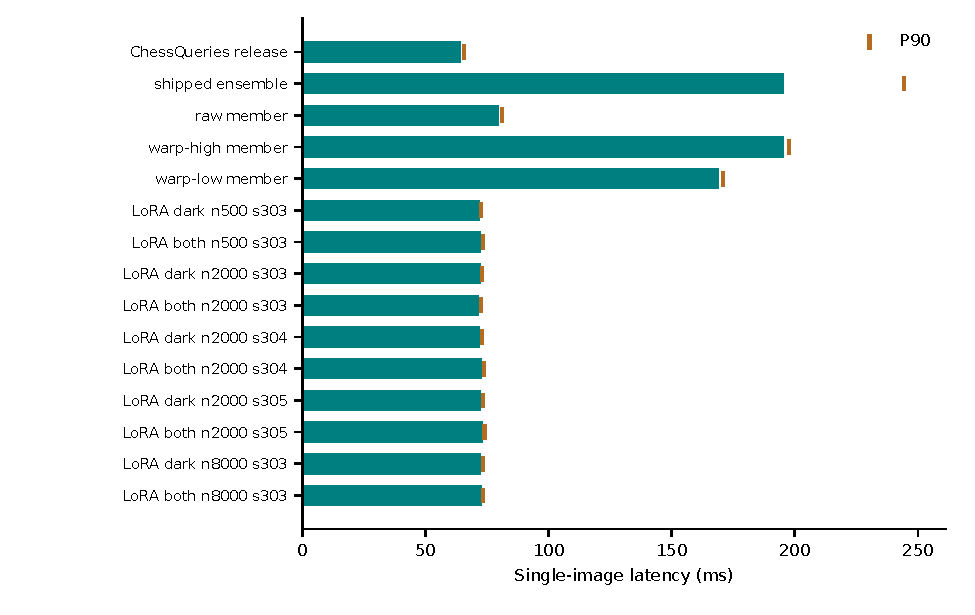
\includegraphics[width=\linewidth]{figures/timing.pdf}
\caption{Single-image synchronized latency. Bars show medians; markers show upper-decile latency. This experiment does not compare accuracy.}\label{fig:timing}
\end{figure}

\section{Limitations and threats to validity}
\label{sec:limitations}

\paragraph{Development data on our own lineage.} Every v2 model result in this paper is on the
400-group development partition of a benchmark rendered by our own generator. Adaptation trains on
a joint mix of factor levels while evaluation reads conditional panels, so a cell result is not the
effect of that factor alone on a model trained without it. The 100-group partition is unscored by
us and its hashes are committed before release; after release, the manifests, seeds,
assets and generator make its pixels reconstructible, so it is an author-unscored split, not a
hidden challenge set.

\paragraph{Real photographs were scored during development.} SLCC, CVChess and ChessReD were each
scored several times while the systems were being built, and ChessCog is itself rendered. Their
numbers are development numbers. No untouched real-photo anchor is part of this version.

\paragraph{Historical provenance.} The v1 spine (Section~\ref{sec:router}) rests on hash-pinned
summary reports whose original execution receipts were not retained; the v1 freeze also records a
stale source revision. Appendix~\ref{app:receipts} lists the receipts and result summaries in this package; the per-image
prediction files behind Section~\ref{sec:lies} are not among them. We did not rebuild those runs.

\paragraph{Independent units.} Benchmark v2 has 400 development position groups, not 16{,}000
independent boards; cells share positions by design, and reference views are shared across panels.
Every interval is a paired bootstrap over position groups. Seed spread at the 2{,}000-position
budget is about one exact point in the dark-only arm and about three in the both-convention arm.

\paragraph{One architecture, one adapter, matched positions not matched images.} The adaptation
study uses one recogniser and the authors' LoRA implementation with upstream optimiser settings and
a fixed update count. Arms match position pools and optimiser presentations, not the number of
available rendered images. The retention-gate failure does not show that every adaptation method
must fail, and the cause of the retention loss is unresolved.

\paragraph{Conditional statistics.} Detector localisation summaries exclude divergent detections,
and that fraction is itself factor-dependent; we publish it beside every summary and make no
``no effect'' claim without a predefined margin.

\paragraph{Licensing and packaging.} Seven of eight piece families carry verified CC0 source
grants. One is CC-BY with its version not displayed by the source page; it is credited by name
and source, and we apply the CC BY 4.0 attribution terms to it. Two families with no licence grant were
excluded from every split. Project code, vendored third-party code, rendered data, the upstream
base weights (non-commercial) and our adapters are separate licensing questions. The first three now have
licence files in the prepared package; the base weights will be linked rather than redistributed,
and the adapters are withheld.

\section{Release package}
\label{sec:release}

The release package is a sanitised export of the author's repository. Identifiers of private
machines and paths are replaced, and digests of the unredacted form of rewritten files are withheld. The package contains the
generator and renderers, the v2 manifests and freeze receipts, the adaptation-pool manifests, the
scoring and diagnostic tools, the figure pipeline that produced every generated figure and table in
this paper from receipts, the licence register (Tables~\ref{tab:licences} and~\ref{tab:datasetlicences}), and the convention table. The paper source and PDF are in the package. The licence
map splits the package by material class: the generator and renderers are source-available under a
noncommercial licence (PolyForm Noncommercial 1.0.0); the scoring, diagnostic and export tools are
Apache-2.0; manifests, receipts, hash lists and rendered images are CC BY-NC 4.0, with attribution to
each piece family's creator; the paper text, figures and tables are CC BY-NC 4.0 and the paper's build
scripts are Apache-2.0; an added permission lets anyone, companies included, evaluate models on the
benchmark and publish the scores; vendored third-party code keeps its upstream notices; the upstream base weights are
non-commercial and are linked, not redistributed; the adapters derive from those weights and are
withheld.

The manifest rows of the 100-group test partition (positions, seeds, cameras and image
hashes) are in the package. Its images are not, and the author scored no model on it. Anyone can
rebuild its pixels from the manifest and the generator, so it is unscored, not hidden
(Section~\ref{sec:limitations}). Images published later can be checked against the image hashes in
the manifest.

Every number in the generated tables carries a source comment naming
its receipt. The package README gives a bounded reproduction path: install, re-render four
benchmark images and compare their hashes, then score them with the public baseline on CPU. It does
not re-render the full benchmark and does not rerun adaptation training. The earlier private systems
are reported from their pinned summaries and are not redistributed. Private material used during
development, including the leaderboard those systems were tuned on, is not part of the release.


\bibliographystyle{plainnat}
\bibliography{references}

\clearpage
\appendix
\section{Full cell results}
\label{app:cells}

Table~\ref{tab:percell} contains every development factor cell for the
release checkpoint and every registered adaptation run. Entries are generated
directly from the copied report receipt; no unsuccessful run or cell is removed.
Percentages in these tables use decimal half-up rounding to two places;
retention decisions use the unrounded recorded values. These are point-estimate tables. The accompanying machine-readable report also
contains the registered paired intervals and gained/lost counts; no between-arm
interval is claimed by the plotted seed spread.

\begingroup\small
\setlength{\tabcolsep}{4pt}
\begin{longtable}{l>{\raggedright\arraybackslash}p{.42\linewidth}rrr}
\caption{Complete development cell results for the release and each adaptation run.}\label{tab:percell}\\
\toprule
Run & % receipt: evidence/tools/reports/paper/lora_curve_2026-09-10/lora_report.complete.json; source: evidence/tools/reports/paper/lora_curve_2026-09-10/lora_report.json; column definitions
Cell / convention & % receipt: evidence/tools/reports/paper/lora_curve_2026-09-10/lora_report.complete.json; source: evidence/tools/reports/paper/lora_curve_2026-09-10/lora_report.json; column definitions
N & % receipt: evidence/tools/reports/paper/lora_curve_2026-09-10/lora_report.complete.json; source: evidence/tools/reports/paper/lora_curve_2026-09-10/lora_report.json; column definitions
Exact (\%) & % receipt: evidence/tools/reports/paper/lora_curve_2026-09-10/lora_report.complete.json; source: evidence/tools/reports/paper/lora_curve_2026-09-10/lora_report.json; column definitions
Square (\%) \\ % receipt: evidence/tools/reports/paper/lora_curve_2026-09-10/lora_report.complete.json; source: evidence/tools/reports/paper/lora_curve_2026-09-10/lora_report.json; column definitions
\midrule

\endfirsthead
\toprule
Run & % receipt: evidence/tools/reports/paper/lora_curve_2026-09-10/lora_report.complete.json; source: evidence/tools/reports/paper/lora_curve_2026-09-10/lora_report.json; column definitions
Cell / convention & % receipt: evidence/tools/reports/paper/lora_curve_2026-09-10/lora_report.complete.json; source: evidence/tools/reports/paper/lora_curve_2026-09-10/lora_report.json; column definitions
N & % receipt: evidence/tools/reports/paper/lora_curve_2026-09-10/lora_report.complete.json; source: evidence/tools/reports/paper/lora_curve_2026-09-10/lora_report.json; column definitions
Exact (\%) & % receipt: evidence/tools/reports/paper/lora_curve_2026-09-10/lora_report.complete.json; source: evidence/tools/reports/paper/lora_curve_2026-09-10/lora_report.json; column definitions
Square (\%) \\ % receipt: evidence/tools/reports/paper/lora_curve_2026-09-10/lora_report.complete.json; source: evidence/tools/reports/paper/lora_curve_2026-09-10/lora_report.json; column definitions
\midrule

\endhead
\bottomrule\endfoot
release & % receipt: evidence/tools/reports/paper/lora_curve_2026-09-10/lora_report.complete.json; source: evidence/tools/reports/paper/lora_curve_2026-09-10/lora_report.json; release/metrics/dev/by_factor_cell_parity/elevation:08_15/a1_dark
elevation:08\_\allowbreak{}15/dark & % receipt: evidence/tools/reports/paper/lora_curve_2026-09-10/lora_report.complete.json; source: evidence/tools/reports/paper/lora_curve_2026-09-10/lora_report.json; release/metrics/dev/by_factor_cell_parity/elevation:08_15/a1_dark
400 & % receipt: evidence/tools/reports/paper/lora_curve_2026-09-10/lora_report.complete.json; source: evidence/tools/reports/paper/lora_curve_2026-09-10/lora_report.json; release/metrics/dev/by_factor_cell_parity/elevation:08_15/a1_dark
0.00 & % receipt: evidence/tools/reports/paper/lora_curve_2026-09-10/lora_report.complete.json; source: evidence/tools/reports/paper/lora_curve_2026-09-10/lora_report.json; release/metrics/dev/by_factor_cell_parity/elevation:08_15/a1_dark
75.04 \\ % receipt: evidence/tools/reports/paper/lora_curve_2026-09-10/lora_report.complete.json; source: evidence/tools/reports/paper/lora_curve_2026-09-10/lora_report.json; release/metrics/dev/by_factor_cell_parity/elevation:08_15/a1_dark

release & % receipt: evidence/tools/reports/paper/lora_curve_2026-09-10/lora_report.complete.json; source: evidence/tools/reports/paper/lora_curve_2026-09-10/lora_report.json; release/metrics/dev/by_factor_cell_parity/elevation:08_15/a1_light
elevation:08\_\allowbreak{}15/light & % receipt: evidence/tools/reports/paper/lora_curve_2026-09-10/lora_report.complete.json; source: evidence/tools/reports/paper/lora_curve_2026-09-10/lora_report.json; release/metrics/dev/by_factor_cell_parity/elevation:08_15/a1_light
400 & % receipt: evidence/tools/reports/paper/lora_curve_2026-09-10/lora_report.complete.json; source: evidence/tools/reports/paper/lora_curve_2026-09-10/lora_report.json; release/metrics/dev/by_factor_cell_parity/elevation:08_15/a1_light
0.00 & % receipt: evidence/tools/reports/paper/lora_curve_2026-09-10/lora_report.complete.json; source: evidence/tools/reports/paper/lora_curve_2026-09-10/lora_report.json; release/metrics/dev/by_factor_cell_parity/elevation:08_15/a1_light
57.89 \\ % receipt: evidence/tools/reports/paper/lora_curve_2026-09-10/lora_report.complete.json; source: evidence/tools/reports/paper/lora_curve_2026-09-10/lora_report.json; release/metrics/dev/by_factor_cell_parity/elevation:08_15/a1_light

release & % receipt: evidence/tools/reports/paper/lora_curve_2026-09-10/lora_report.complete.json; source: evidence/tools/reports/paper/lora_curve_2026-09-10/lora_report.json; release/metrics/dev/by_factor_cell_parity/elevation:15_25/a1_dark
elevation:15\_\allowbreak{}25/dark & % receipt: evidence/tools/reports/paper/lora_curve_2026-09-10/lora_report.complete.json; source: evidence/tools/reports/paper/lora_curve_2026-09-10/lora_report.json; release/metrics/dev/by_factor_cell_parity/elevation:15_25/a1_dark
400 & % receipt: evidence/tools/reports/paper/lora_curve_2026-09-10/lora_report.complete.json; source: evidence/tools/reports/paper/lora_curve_2026-09-10/lora_report.json; release/metrics/dev/by_factor_cell_parity/elevation:15_25/a1_dark
5.75 & % receipt: evidence/tools/reports/paper/lora_curve_2026-09-10/lora_report.complete.json; source: evidence/tools/reports/paper/lora_curve_2026-09-10/lora_report.json; release/metrics/dev/by_factor_cell_parity/elevation:15_25/a1_dark
88.21 \\ % receipt: evidence/tools/reports/paper/lora_curve_2026-09-10/lora_report.complete.json; source: evidence/tools/reports/paper/lora_curve_2026-09-10/lora_report.json; release/metrics/dev/by_factor_cell_parity/elevation:15_25/a1_dark

release & % receipt: evidence/tools/reports/paper/lora_curve_2026-09-10/lora_report.complete.json; source: evidence/tools/reports/paper/lora_curve_2026-09-10/lora_report.json; release/metrics/dev/by_factor_cell_parity/elevation:15_25/a1_light
elevation:15\_\allowbreak{}25/light & % receipt: evidence/tools/reports/paper/lora_curve_2026-09-10/lora_report.complete.json; source: evidence/tools/reports/paper/lora_curve_2026-09-10/lora_report.json; release/metrics/dev/by_factor_cell_parity/elevation:15_25/a1_light
400 & % receipt: evidence/tools/reports/paper/lora_curve_2026-09-10/lora_report.complete.json; source: evidence/tools/reports/paper/lora_curve_2026-09-10/lora_report.json; release/metrics/dev/by_factor_cell_parity/elevation:15_25/a1_light
0.00 & % receipt: evidence/tools/reports/paper/lora_curve_2026-09-10/lora_report.complete.json; source: evidence/tools/reports/paper/lora_curve_2026-09-10/lora_report.json; release/metrics/dev/by_factor_cell_parity/elevation:15_25/a1_light
56.19 \\ % receipt: evidence/tools/reports/paper/lora_curve_2026-09-10/lora_report.complete.json; source: evidence/tools/reports/paper/lora_curve_2026-09-10/lora_report.json; release/metrics/dev/by_factor_cell_parity/elevation:15_25/a1_light

release & % receipt: evidence/tools/reports/paper/lora_curve_2026-09-10/lora_report.complete.json; source: evidence/tools/reports/paper/lora_curve_2026-09-10/lora_report.json; release/metrics/dev/by_factor_cell_parity/elevation:25_45/a1_dark
elevation:25\_\allowbreak{}45/dark & % receipt: evidence/tools/reports/paper/lora_curve_2026-09-10/lora_report.complete.json; source: evidence/tools/reports/paper/lora_curve_2026-09-10/lora_report.json; release/metrics/dev/by_factor_cell_parity/elevation:25_45/a1_dark
400 & % receipt: evidence/tools/reports/paper/lora_curve_2026-09-10/lora_report.complete.json; source: evidence/tools/reports/paper/lora_curve_2026-09-10/lora_report.json; release/metrics/dev/by_factor_cell_parity/elevation:25_45/a1_dark
18.00 & % receipt: evidence/tools/reports/paper/lora_curve_2026-09-10/lora_report.complete.json; source: evidence/tools/reports/paper/lora_curve_2026-09-10/lora_report.json; release/metrics/dev/by_factor_cell_parity/elevation:25_45/a1_dark
87.28 \\ % receipt: evidence/tools/reports/paper/lora_curve_2026-09-10/lora_report.complete.json; source: evidence/tools/reports/paper/lora_curve_2026-09-10/lora_report.json; release/metrics/dev/by_factor_cell_parity/elevation:25_45/a1_dark

release & % receipt: evidence/tools/reports/paper/lora_curve_2026-09-10/lora_report.complete.json; source: evidence/tools/reports/paper/lora_curve_2026-09-10/lora_report.json; release/metrics/dev/by_factor_cell_parity/elevation:25_45/a1_light
elevation:25\_\allowbreak{}45/light & % receipt: evidence/tools/reports/paper/lora_curve_2026-09-10/lora_report.complete.json; source: evidence/tools/reports/paper/lora_curve_2026-09-10/lora_report.json; release/metrics/dev/by_factor_cell_parity/elevation:25_45/a1_light
400 & % receipt: evidence/tools/reports/paper/lora_curve_2026-09-10/lora_report.complete.json; source: evidence/tools/reports/paper/lora_curve_2026-09-10/lora_report.json; release/metrics/dev/by_factor_cell_parity/elevation:25_45/a1_light
0.00 & % receipt: evidence/tools/reports/paper/lora_curve_2026-09-10/lora_report.complete.json; source: evidence/tools/reports/paper/lora_curve_2026-09-10/lora_report.json; release/metrics/dev/by_factor_cell_parity/elevation:25_45/a1_light
53.94 \\ % receipt: evidence/tools/reports/paper/lora_curve_2026-09-10/lora_report.complete.json; source: evidence/tools/reports/paper/lora_curve_2026-09-10/lora_report.json; release/metrics/dev/by_factor_cell_parity/elevation:25_45/a1_light

release & % receipt: evidence/tools/reports/paper/lora_curve_2026-09-10/lora_report.complete.json; source: evidence/tools/reports/paper/lora_curve_2026-09-10/lora_report.json; release/metrics/dev/by_factor_cell_parity/elevation:45_60/a1_dark
elevation:45\_\allowbreak{}60/dark & % receipt: evidence/tools/reports/paper/lora_curve_2026-09-10/lora_report.complete.json; source: evidence/tools/reports/paper/lora_curve_2026-09-10/lora_report.json; release/metrics/dev/by_factor_cell_parity/elevation:45_60/a1_dark
400 & % receipt: evidence/tools/reports/paper/lora_curve_2026-09-10/lora_report.complete.json; source: evidence/tools/reports/paper/lora_curve_2026-09-10/lora_report.json; release/metrics/dev/by_factor_cell_parity/elevation:45_60/a1_dark
14.25 & % receipt: evidence/tools/reports/paper/lora_curve_2026-09-10/lora_report.complete.json; source: evidence/tools/reports/paper/lora_curve_2026-09-10/lora_report.json; release/metrics/dev/by_factor_cell_parity/elevation:45_60/a1_dark
84.19 \\ % receipt: evidence/tools/reports/paper/lora_curve_2026-09-10/lora_report.complete.json; source: evidence/tools/reports/paper/lora_curve_2026-09-10/lora_report.json; release/metrics/dev/by_factor_cell_parity/elevation:45_60/a1_dark

release & % receipt: evidence/tools/reports/paper/lora_curve_2026-09-10/lora_report.complete.json; source: evidence/tools/reports/paper/lora_curve_2026-09-10/lora_report.json; release/metrics/dev/by_factor_cell_parity/elevation:45_60/a1_light
elevation:45\_\allowbreak{}60/light & % receipt: evidence/tools/reports/paper/lora_curve_2026-09-10/lora_report.complete.json; source: evidence/tools/reports/paper/lora_curve_2026-09-10/lora_report.json; release/metrics/dev/by_factor_cell_parity/elevation:45_60/a1_light
400 & % receipt: evidence/tools/reports/paper/lora_curve_2026-09-10/lora_report.complete.json; source: evidence/tools/reports/paper/lora_curve_2026-09-10/lora_report.json; release/metrics/dev/by_factor_cell_parity/elevation:45_60/a1_light
0.00 & % receipt: evidence/tools/reports/paper/lora_curve_2026-09-10/lora_report.complete.json; source: evidence/tools/reports/paper/lora_curve_2026-09-10/lora_report.json; release/metrics/dev/by_factor_cell_parity/elevation:45_60/a1_light
52.89 \\ % receipt: evidence/tools/reports/paper/lora_curve_2026-09-10/lora_report.complete.json; source: evidence/tools/reports/paper/lora_curve_2026-09-10/lora_report.json; release/metrics/dev/by_factor_cell_parity/elevation:45_60/a1_light

release & % receipt: evidence/tools/reports/paper/lora_curve_2026-09-10/lora_report.complete.json; source: evidence/tools/reports/paper/lora_curve_2026-09-10/lora_report.json; release/metrics/dev/by_factor_cell_parity/framing:compact/a1_dark
framing:compact/dark & % receipt: evidence/tools/reports/paper/lora_curve_2026-09-10/lora_report.complete.json; source: evidence/tools/reports/paper/lora_curve_2026-09-10/lora_report.json; release/metrics/dev/by_factor_cell_parity/framing:compact/a1_dark
400 & % receipt: evidence/tools/reports/paper/lora_curve_2026-09-10/lora_report.complete.json; source: evidence/tools/reports/paper/lora_curve_2026-09-10/lora_report.json; release/metrics/dev/by_factor_cell_parity/framing:compact/a1_dark
7.25 & % receipt: evidence/tools/reports/paper/lora_curve_2026-09-10/lora_report.complete.json; source: evidence/tools/reports/paper/lora_curve_2026-09-10/lora_report.json; release/metrics/dev/by_factor_cell_parity/framing:compact/a1_dark
85.01 \\ % receipt: evidence/tools/reports/paper/lora_curve_2026-09-10/lora_report.complete.json; source: evidence/tools/reports/paper/lora_curve_2026-09-10/lora_report.json; release/metrics/dev/by_factor_cell_parity/framing:compact/a1_dark

release & % receipt: evidence/tools/reports/paper/lora_curve_2026-09-10/lora_report.complete.json; source: evidence/tools/reports/paper/lora_curve_2026-09-10/lora_report.json; release/metrics/dev/by_factor_cell_parity/framing:compact/a1_light
framing:compact/light & % receipt: evidence/tools/reports/paper/lora_curve_2026-09-10/lora_report.complete.json; source: evidence/tools/reports/paper/lora_curve_2026-09-10/lora_report.json; release/metrics/dev/by_factor_cell_parity/framing:compact/a1_light
400 & % receipt: evidence/tools/reports/paper/lora_curve_2026-09-10/lora_report.complete.json; source: evidence/tools/reports/paper/lora_curve_2026-09-10/lora_report.json; release/metrics/dev/by_factor_cell_parity/framing:compact/a1_light
0.00 & % receipt: evidence/tools/reports/paper/lora_curve_2026-09-10/lora_report.complete.json; source: evidence/tools/reports/paper/lora_curve_2026-09-10/lora_report.json; release/metrics/dev/by_factor_cell_parity/framing:compact/a1_light
52.18 \\ % receipt: evidence/tools/reports/paper/lora_curve_2026-09-10/lora_report.complete.json; source: evidence/tools/reports/paper/lora_curve_2026-09-10/lora_report.json; release/metrics/dev/by_factor_cell_parity/framing:compact/a1_light

release & % receipt: evidence/tools/reports/paper/lora_curve_2026-09-10/lora_report.complete.json; source: evidence/tools/reports/paper/lora_curve_2026-09-10/lora_report.json; release/metrics/dev/by_factor_cell_parity/framing:standard/a1_dark
framing:standard/dark & % receipt: evidence/tools/reports/paper/lora_curve_2026-09-10/lora_report.complete.json; source: evidence/tools/reports/paper/lora_curve_2026-09-10/lora_report.json; release/metrics/dev/by_factor_cell_parity/framing:standard/a1_dark
400 & % receipt: evidence/tools/reports/paper/lora_curve_2026-09-10/lora_report.complete.json; source: evidence/tools/reports/paper/lora_curve_2026-09-10/lora_report.json; release/metrics/dev/by_factor_cell_parity/framing:standard/a1_dark
14.25 & % receipt: evidence/tools/reports/paper/lora_curve_2026-09-10/lora_report.complete.json; source: evidence/tools/reports/paper/lora_curve_2026-09-10/lora_report.json; release/metrics/dev/by_factor_cell_parity/framing:standard/a1_dark
84.19 \\ % receipt: evidence/tools/reports/paper/lora_curve_2026-09-10/lora_report.complete.json; source: evidence/tools/reports/paper/lora_curve_2026-09-10/lora_report.json; release/metrics/dev/by_factor_cell_parity/framing:standard/a1_dark

release & % receipt: evidence/tools/reports/paper/lora_curve_2026-09-10/lora_report.complete.json; source: evidence/tools/reports/paper/lora_curve_2026-09-10/lora_report.json; release/metrics/dev/by_factor_cell_parity/framing:standard/a1_light
framing:standard/light & % receipt: evidence/tools/reports/paper/lora_curve_2026-09-10/lora_report.complete.json; source: evidence/tools/reports/paper/lora_curve_2026-09-10/lora_report.json; release/metrics/dev/by_factor_cell_parity/framing:standard/a1_light
400 & % receipt: evidence/tools/reports/paper/lora_curve_2026-09-10/lora_report.complete.json; source: evidence/tools/reports/paper/lora_curve_2026-09-10/lora_report.json; release/metrics/dev/by_factor_cell_parity/framing:standard/a1_light
0.00 & % receipt: evidence/tools/reports/paper/lora_curve_2026-09-10/lora_report.complete.json; source: evidence/tools/reports/paper/lora_curve_2026-09-10/lora_report.json; release/metrics/dev/by_factor_cell_parity/framing:standard/a1_light
52.89 \\ % receipt: evidence/tools/reports/paper/lora_curve_2026-09-10/lora_report.complete.json; source: evidence/tools/reports/paper/lora_curve_2026-09-10/lora_report.json; release/metrics/dev/by_factor_cell_parity/framing:standard/a1_light

release & % receipt: evidence/tools/reports/paper/lora_curve_2026-09-10/lora_report.complete.json; source: evidence/tools/reports/paper/lora_curve_2026-09-10/lora_report.json; release/metrics/dev/by_factor_cell_parity/geometry:deplorable/a1_dark
geometry:deplorable/dark & % receipt: evidence/tools/reports/paper/lora_curve_2026-09-10/lora_report.complete.json; source: evidence/tools/reports/paper/lora_curve_2026-09-10/lora_report.json; release/metrics/dev/by_factor_cell_parity/geometry:deplorable/a1_dark
400 & % receipt: evidence/tools/reports/paper/lora_curve_2026-09-10/lora_report.complete.json; source: evidence/tools/reports/paper/lora_curve_2026-09-10/lora_report.json; release/metrics/dev/by_factor_cell_parity/geometry:deplorable/a1_dark
34.25 & % receipt: evidence/tools/reports/paper/lora_curve_2026-09-10/lora_report.complete.json; source: evidence/tools/reports/paper/lora_curve_2026-09-10/lora_report.json; release/metrics/dev/by_factor_cell_parity/geometry:deplorable/a1_dark
86.95 \\ % receipt: evidence/tools/reports/paper/lora_curve_2026-09-10/lora_report.complete.json; source: evidence/tools/reports/paper/lora_curve_2026-09-10/lora_report.json; release/metrics/dev/by_factor_cell_parity/geometry:deplorable/a1_dark

release & % receipt: evidence/tools/reports/paper/lora_curve_2026-09-10/lora_report.complete.json; source: evidence/tools/reports/paper/lora_curve_2026-09-10/lora_report.json; release/metrics/dev/by_factor_cell_parity/geometry:deplorable/a1_light
geometry:deplorable/light & % receipt: evidence/tools/reports/paper/lora_curve_2026-09-10/lora_report.complete.json; source: evidence/tools/reports/paper/lora_curve_2026-09-10/lora_report.json; release/metrics/dev/by_factor_cell_parity/geometry:deplorable/a1_light
400 & % receipt: evidence/tools/reports/paper/lora_curve_2026-09-10/lora_report.complete.json; source: evidence/tools/reports/paper/lora_curve_2026-09-10/lora_report.json; release/metrics/dev/by_factor_cell_parity/geometry:deplorable/a1_light
0.00 & % receipt: evidence/tools/reports/paper/lora_curve_2026-09-10/lora_report.complete.json; source: evidence/tools/reports/paper/lora_curve_2026-09-10/lora_report.json; release/metrics/dev/by_factor_cell_parity/geometry:deplorable/a1_light
53.63 \\ % receipt: evidence/tools/reports/paper/lora_curve_2026-09-10/lora_report.complete.json; source: evidence/tools/reports/paper/lora_curve_2026-09-10/lora_report.json; release/metrics/dev/by_factor_cell_parity/geometry:deplorable/a1_light

release & % receipt: evidence/tools/reports/paper/lora_curve_2026-09-10/lora_report.complete.json; source: evidence/tools/reports/paper/lora_curve_2026-09-10/lora_report.json; release/metrics/dev/by_factor_cell_parity/geometry:killgorack/a1_dark
geometry:killgorack/dark & % receipt: evidence/tools/reports/paper/lora_curve_2026-09-10/lora_report.complete.json; source: evidence/tools/reports/paper/lora_curve_2026-09-10/lora_report.json; release/metrics/dev/by_factor_cell_parity/geometry:killgorack/a1_dark
400 & % receipt: evidence/tools/reports/paper/lora_curve_2026-09-10/lora_report.complete.json; source: evidence/tools/reports/paper/lora_curve_2026-09-10/lora_report.json; release/metrics/dev/by_factor_cell_parity/geometry:killgorack/a1_dark
25.75 & % receipt: evidence/tools/reports/paper/lora_curve_2026-09-10/lora_report.complete.json; source: evidence/tools/reports/paper/lora_curve_2026-09-10/lora_report.json; release/metrics/dev/by_factor_cell_parity/geometry:killgorack/a1_dark
85.27 \\ % receipt: evidence/tools/reports/paper/lora_curve_2026-09-10/lora_report.complete.json; source: evidence/tools/reports/paper/lora_curve_2026-09-10/lora_report.json; release/metrics/dev/by_factor_cell_parity/geometry:killgorack/a1_dark

release & % receipt: evidence/tools/reports/paper/lora_curve_2026-09-10/lora_report.complete.json; source: evidence/tools/reports/paper/lora_curve_2026-09-10/lora_report.json; release/metrics/dev/by_factor_cell_parity/geometry:killgorack/a1_light
geometry:killgorack/light & % receipt: evidence/tools/reports/paper/lora_curve_2026-09-10/lora_report.complete.json; source: evidence/tools/reports/paper/lora_curve_2026-09-10/lora_report.json; release/metrics/dev/by_factor_cell_parity/geometry:killgorack/a1_light
400 & % receipt: evidence/tools/reports/paper/lora_curve_2026-09-10/lora_report.complete.json; source: evidence/tools/reports/paper/lora_curve_2026-09-10/lora_report.json; release/metrics/dev/by_factor_cell_parity/geometry:killgorack/a1_light
0.00 & % receipt: evidence/tools/reports/paper/lora_curve_2026-09-10/lora_report.complete.json; source: evidence/tools/reports/paper/lora_curve_2026-09-10/lora_report.json; release/metrics/dev/by_factor_cell_parity/geometry:killgorack/a1_light
53.81 \\ % receipt: evidence/tools/reports/paper/lora_curve_2026-09-10/lora_report.complete.json; source: evidence/tools/reports/paper/lora_curve_2026-09-10/lora_report.json; release/metrics/dev/by_factor_cell_parity/geometry:killgorack/a1_light

release & % receipt: evidence/tools/reports/paper/lora_curve_2026-09-10/lora_report.complete.json; source: evidence/tools/reports/paper/lora_curve_2026-09-10/lora_report.json; release/metrics/dev/by_factor_cell_parity/geometry:lyricsz/a1_dark
geometry:lyricsz/dark & % receipt: evidence/tools/reports/paper/lora_curve_2026-09-10/lora_report.complete.json; source: evidence/tools/reports/paper/lora_curve_2026-09-10/lora_report.json; release/metrics/dev/by_factor_cell_parity/geometry:lyricsz/a1_dark
400 & % receipt: evidence/tools/reports/paper/lora_curve_2026-09-10/lora_report.complete.json; source: evidence/tools/reports/paper/lora_curve_2026-09-10/lora_report.json; release/metrics/dev/by_factor_cell_parity/geometry:lyricsz/a1_dark
3.00 & % receipt: evidence/tools/reports/paper/lora_curve_2026-09-10/lora_report.complete.json; source: evidence/tools/reports/paper/lora_curve_2026-09-10/lora_report.json; release/metrics/dev/by_factor_cell_parity/geometry:lyricsz/a1_dark
83.43 \\ % receipt: evidence/tools/reports/paper/lora_curve_2026-09-10/lora_report.complete.json; source: evidence/tools/reports/paper/lora_curve_2026-09-10/lora_report.json; release/metrics/dev/by_factor_cell_parity/geometry:lyricsz/a1_dark

release & % receipt: evidence/tools/reports/paper/lora_curve_2026-09-10/lora_report.complete.json; source: evidence/tools/reports/paper/lora_curve_2026-09-10/lora_report.json; release/metrics/dev/by_factor_cell_parity/geometry:lyricsz/a1_light
geometry:lyricsz/light & % receipt: evidence/tools/reports/paper/lora_curve_2026-09-10/lora_report.complete.json; source: evidence/tools/reports/paper/lora_curve_2026-09-10/lora_report.json; release/metrics/dev/by_factor_cell_parity/geometry:lyricsz/a1_light
400 & % receipt: evidence/tools/reports/paper/lora_curve_2026-09-10/lora_report.complete.json; source: evidence/tools/reports/paper/lora_curve_2026-09-10/lora_report.json; release/metrics/dev/by_factor_cell_parity/geometry:lyricsz/a1_light
0.00 & % receipt: evidence/tools/reports/paper/lora_curve_2026-09-10/lora_report.complete.json; source: evidence/tools/reports/paper/lora_curve_2026-09-10/lora_report.json; release/metrics/dev/by_factor_cell_parity/geometry:lyricsz/a1_light
55.74 \\ % receipt: evidence/tools/reports/paper/lora_curve_2026-09-10/lora_report.complete.json; source: evidence/tools/reports/paper/lora_curve_2026-09-10/lora_report.json; release/metrics/dev/by_factor_cell_parity/geometry:lyricsz/a1_light

release & % receipt: evidence/tools/reports/paper/lora_curve_2026-09-10/lora_report.complete.json; source: evidence/tools/reports/paper/lora_curve_2026-09-10/lora_report.json; release/metrics/dev/by_factor_cell_parity/geometry:nailfighter/a1_dark
geometry:nailfighter/dark & % receipt: evidence/tools/reports/paper/lora_curve_2026-09-10/lora_report.complete.json; source: evidence/tools/reports/paper/lora_curve_2026-09-10/lora_report.json; release/metrics/dev/by_factor_cell_parity/geometry:nailfighter/a1_dark
400 & % receipt: evidence/tools/reports/paper/lora_curve_2026-09-10/lora_report.complete.json; source: evidence/tools/reports/paper/lora_curve_2026-09-10/lora_report.json; release/metrics/dev/by_factor_cell_parity/geometry:nailfighter/a1_dark
25.00 & % receipt: evidence/tools/reports/paper/lora_curve_2026-09-10/lora_report.complete.json; source: evidence/tools/reports/paper/lora_curve_2026-09-10/lora_report.json; release/metrics/dev/by_factor_cell_parity/geometry:nailfighter/a1_dark
87.52 \\ % receipt: evidence/tools/reports/paper/lora_curve_2026-09-10/lora_report.complete.json; source: evidence/tools/reports/paper/lora_curve_2026-09-10/lora_report.json; release/metrics/dev/by_factor_cell_parity/geometry:nailfighter/a1_dark

release & % receipt: evidence/tools/reports/paper/lora_curve_2026-09-10/lora_report.complete.json; source: evidence/tools/reports/paper/lora_curve_2026-09-10/lora_report.json; release/metrics/dev/by_factor_cell_parity/geometry:nailfighter/a1_light
geometry:nailfighter/light & % receipt: evidence/tools/reports/paper/lora_curve_2026-09-10/lora_report.complete.json; source: evidence/tools/reports/paper/lora_curve_2026-09-10/lora_report.json; release/metrics/dev/by_factor_cell_parity/geometry:nailfighter/a1_light
400 & % receipt: evidence/tools/reports/paper/lora_curve_2026-09-10/lora_report.complete.json; source: evidence/tools/reports/paper/lora_curve_2026-09-10/lora_report.json; release/metrics/dev/by_factor_cell_parity/geometry:nailfighter/a1_light
0.00 & % receipt: evidence/tools/reports/paper/lora_curve_2026-09-10/lora_report.complete.json; source: evidence/tools/reports/paper/lora_curve_2026-09-10/lora_report.json; release/metrics/dev/by_factor_cell_parity/geometry:nailfighter/a1_light
54.04 \\ % receipt: evidence/tools/reports/paper/lora_curve_2026-09-10/lora_report.complete.json; source: evidence/tools/reports/paper/lora_curve_2026-09-10/lora_report.json; release/metrics/dev/by_factor_cell_parity/geometry:nailfighter/a1_light

release & % receipt: evidence/tools/reports/paper/lora_curve_2026-09-10/lora_report.complete.json; source: evidence/tools/reports/paper/lora_curve_2026-09-10/lora_report.json; release/metrics/dev/by_factor_cell_parity/geometry:omie/a1_dark
geometry:omie/dark & % receipt: evidence/tools/reports/paper/lora_curve_2026-09-10/lora_report.complete.json; source: evidence/tools/reports/paper/lora_curve_2026-09-10/lora_report.json; release/metrics/dev/by_factor_cell_parity/geometry:omie/a1_dark
400 & % receipt: evidence/tools/reports/paper/lora_curve_2026-09-10/lora_report.complete.json; source: evidence/tools/reports/paper/lora_curve_2026-09-10/lora_report.json; release/metrics/dev/by_factor_cell_parity/geometry:omie/a1_dark
34.25 & % receipt: evidence/tools/reports/paper/lora_curve_2026-09-10/lora_report.complete.json; source: evidence/tools/reports/paper/lora_curve_2026-09-10/lora_report.json; release/metrics/dev/by_factor_cell_parity/geometry:omie/a1_dark
88.35 \\ % receipt: evidence/tools/reports/paper/lora_curve_2026-09-10/lora_report.complete.json; source: evidence/tools/reports/paper/lora_curve_2026-09-10/lora_report.json; release/metrics/dev/by_factor_cell_parity/geometry:omie/a1_dark

release & % receipt: evidence/tools/reports/paper/lora_curve_2026-09-10/lora_report.complete.json; source: evidence/tools/reports/paper/lora_curve_2026-09-10/lora_report.json; release/metrics/dev/by_factor_cell_parity/geometry:omie/a1_light
geometry:omie/light & % receipt: evidence/tools/reports/paper/lora_curve_2026-09-10/lora_report.complete.json; source: evidence/tools/reports/paper/lora_curve_2026-09-10/lora_report.json; release/metrics/dev/by_factor_cell_parity/geometry:omie/a1_light
400 & % receipt: evidence/tools/reports/paper/lora_curve_2026-09-10/lora_report.complete.json; source: evidence/tools/reports/paper/lora_curve_2026-09-10/lora_report.json; release/metrics/dev/by_factor_cell_parity/geometry:omie/a1_light
0.00 & % receipt: evidence/tools/reports/paper/lora_curve_2026-09-10/lora_report.complete.json; source: evidence/tools/reports/paper/lora_curve_2026-09-10/lora_report.json; release/metrics/dev/by_factor_cell_parity/geometry:omie/a1_light
54.60 \\ % receipt: evidence/tools/reports/paper/lora_curve_2026-09-10/lora_report.complete.json; source: evidence/tools/reports/paper/lora_curve_2026-09-10/lora_report.json; release/metrics/dev/by_factor_cell_parity/geometry:omie/a1_light

release & % receipt: evidence/tools/reports/paper/lora_curve_2026-09-10/lora_report.complete.json; source: evidence/tools/reports/paper/lora_curve_2026-09-10/lora_report.json; release/metrics/dev/by_factor_cell_parity/geometry:phuong/a1_dark
geometry:phuong/dark & % receipt: evidence/tools/reports/paper/lora_curve_2026-09-10/lora_report.complete.json; source: evidence/tools/reports/paper/lora_curve_2026-09-10/lora_report.json; release/metrics/dev/by_factor_cell_parity/geometry:phuong/a1_dark
400 & % receipt: evidence/tools/reports/paper/lora_curve_2026-09-10/lora_report.complete.json; source: evidence/tools/reports/paper/lora_curve_2026-09-10/lora_report.json; release/metrics/dev/by_factor_cell_parity/geometry:phuong/a1_dark
17.25 & % receipt: evidence/tools/reports/paper/lora_curve_2026-09-10/lora_report.complete.json; source: evidence/tools/reports/paper/lora_curve_2026-09-10/lora_report.json; release/metrics/dev/by_factor_cell_parity/geometry:phuong/a1_dark
86.04 \\ % receipt: evidence/tools/reports/paper/lora_curve_2026-09-10/lora_report.complete.json; source: evidence/tools/reports/paper/lora_curve_2026-09-10/lora_report.json; release/metrics/dev/by_factor_cell_parity/geometry:phuong/a1_dark

release & % receipt: evidence/tools/reports/paper/lora_curve_2026-09-10/lora_report.complete.json; source: evidence/tools/reports/paper/lora_curve_2026-09-10/lora_report.json; release/metrics/dev/by_factor_cell_parity/geometry:phuong/a1_light
geometry:phuong/light & % receipt: evidence/tools/reports/paper/lora_curve_2026-09-10/lora_report.complete.json; source: evidence/tools/reports/paper/lora_curve_2026-09-10/lora_report.json; release/metrics/dev/by_factor_cell_parity/geometry:phuong/a1_light
400 & % receipt: evidence/tools/reports/paper/lora_curve_2026-09-10/lora_report.complete.json; source: evidence/tools/reports/paper/lora_curve_2026-09-10/lora_report.json; release/metrics/dev/by_factor_cell_parity/geometry:phuong/a1_light
0.00 & % receipt: evidence/tools/reports/paper/lora_curve_2026-09-10/lora_report.complete.json; source: evidence/tools/reports/paper/lora_curve_2026-09-10/lora_report.json; release/metrics/dev/by_factor_cell_parity/geometry:phuong/a1_light
54.87 \\ % receipt: evidence/tools/reports/paper/lora_curve_2026-09-10/lora_report.complete.json; source: evidence/tools/reports/paper/lora_curve_2026-09-10/lora_report.json; release/metrics/dev/by_factor_cell_parity/geometry:phuong/a1_light

release & % receipt: evidence/tools/reports/paper/lora_curve_2026-09-10/lora_report.complete.json; source: evidence/tools/reports/paper/lora_curve_2026-09-10/lora_report.json; release/metrics/dev/by_factor_cell_parity/geometry:pjhanzlik/a1_dark
geometry:pjhanzlik/dark & % receipt: evidence/tools/reports/paper/lora_curve_2026-09-10/lora_report.complete.json; source: evidence/tools/reports/paper/lora_curve_2026-09-10/lora_report.json; release/metrics/dev/by_factor_cell_parity/geometry:pjhanzlik/a1_dark
400 & % receipt: evidence/tools/reports/paper/lora_curve_2026-09-10/lora_report.complete.json; source: evidence/tools/reports/paper/lora_curve_2026-09-10/lora_report.json; release/metrics/dev/by_factor_cell_parity/geometry:pjhanzlik/a1_dark
4.75 & % receipt: evidence/tools/reports/paper/lora_curve_2026-09-10/lora_report.complete.json; source: evidence/tools/reports/paper/lora_curve_2026-09-10/lora_report.json; release/metrics/dev/by_factor_cell_parity/geometry:pjhanzlik/a1_dark
80.97 \\ % receipt: evidence/tools/reports/paper/lora_curve_2026-09-10/lora_report.complete.json; source: evidence/tools/reports/paper/lora_curve_2026-09-10/lora_report.json; release/metrics/dev/by_factor_cell_parity/geometry:pjhanzlik/a1_dark

release & % receipt: evidence/tools/reports/paper/lora_curve_2026-09-10/lora_report.complete.json; source: evidence/tools/reports/paper/lora_curve_2026-09-10/lora_report.json; release/metrics/dev/by_factor_cell_parity/geometry:pjhanzlik/a1_light
geometry:pjhanzlik/light & % receipt: evidence/tools/reports/paper/lora_curve_2026-09-10/lora_report.complete.json; source: evidence/tools/reports/paper/lora_curve_2026-09-10/lora_report.json; release/metrics/dev/by_factor_cell_parity/geometry:pjhanzlik/a1_light
400 & % receipt: evidence/tools/reports/paper/lora_curve_2026-09-10/lora_report.complete.json; source: evidence/tools/reports/paper/lora_curve_2026-09-10/lora_report.json; release/metrics/dev/by_factor_cell_parity/geometry:pjhanzlik/a1_light
0.00 & % receipt: evidence/tools/reports/paper/lora_curve_2026-09-10/lora_report.complete.json; source: evidence/tools/reports/paper/lora_curve_2026-09-10/lora_report.json; release/metrics/dev/by_factor_cell_parity/geometry:pjhanzlik/a1_light
54.66 \\ % receipt: evidence/tools/reports/paper/lora_curve_2026-09-10/lora_report.complete.json; source: evidence/tools/reports/paper/lora_curve_2026-09-10/lora_report.json; release/metrics/dev/by_factor_cell_parity/geometry:pjhanzlik/a1_light

release & % receipt: evidence/tools/reports/paper/lora_curve_2026-09-10/lora_report.complete.json; source: evidence/tools/reports/paper/lora_curve_2026-09-10/lora_report.json; release/metrics/dev/by_factor_cell_parity/geometry:polyhaven/a1_dark
geometry:polyhaven/dark & % receipt: evidence/tools/reports/paper/lora_curve_2026-09-10/lora_report.complete.json; source: evidence/tools/reports/paper/lora_curve_2026-09-10/lora_report.json; release/metrics/dev/by_factor_cell_parity/geometry:polyhaven/a1_dark
400 & % receipt: evidence/tools/reports/paper/lora_curve_2026-09-10/lora_report.complete.json; source: evidence/tools/reports/paper/lora_curve_2026-09-10/lora_report.json; release/metrics/dev/by_factor_cell_parity/geometry:polyhaven/a1_dark
14.25 & % receipt: evidence/tools/reports/paper/lora_curve_2026-09-10/lora_report.complete.json; source: evidence/tools/reports/paper/lora_curve_2026-09-10/lora_report.json; release/metrics/dev/by_factor_cell_parity/geometry:polyhaven/a1_dark
84.19 \\ % receipt: evidence/tools/reports/paper/lora_curve_2026-09-10/lora_report.complete.json; source: evidence/tools/reports/paper/lora_curve_2026-09-10/lora_report.json; release/metrics/dev/by_factor_cell_parity/geometry:polyhaven/a1_dark

release & % receipt: evidence/tools/reports/paper/lora_curve_2026-09-10/lora_report.complete.json; source: evidence/tools/reports/paper/lora_curve_2026-09-10/lora_report.json; release/metrics/dev/by_factor_cell_parity/geometry:polyhaven/a1_light
geometry:polyhaven/light & % receipt: evidence/tools/reports/paper/lora_curve_2026-09-10/lora_report.complete.json; source: evidence/tools/reports/paper/lora_curve_2026-09-10/lora_report.json; release/metrics/dev/by_factor_cell_parity/geometry:polyhaven/a1_light
400 & % receipt: evidence/tools/reports/paper/lora_curve_2026-09-10/lora_report.complete.json; source: evidence/tools/reports/paper/lora_curve_2026-09-10/lora_report.json; release/metrics/dev/by_factor_cell_parity/geometry:polyhaven/a1_light
0.00 & % receipt: evidence/tools/reports/paper/lora_curve_2026-09-10/lora_report.complete.json; source: evidence/tools/reports/paper/lora_curve_2026-09-10/lora_report.json; release/metrics/dev/by_factor_cell_parity/geometry:polyhaven/a1_light
52.89 \\ % receipt: evidence/tools/reports/paper/lora_curve_2026-09-10/lora_report.complete.json; source: evidence/tools/reports/paper/lora_curve_2026-09-10/lora_report.json; release/metrics/dev/by_factor_cell_parity/geometry:polyhaven/a1_light

release & % receipt: evidence/tools/reports/paper/lora_curve_2026-09-10/lora_report.complete.json; source: evidence/tools/reports/paper/lora_curve_2026-09-10/lora_report.json; release/metrics/dev/by_factor_cell_parity/palette:aubergine_periwinkle/a1_dark
palette:aubergine\_\allowbreak{}periwinkle/dark & % receipt: evidence/tools/reports/paper/lora_curve_2026-09-10/lora_report.complete.json; source: evidence/tools/reports/paper/lora_curve_2026-09-10/lora_report.json; release/metrics/dev/by_factor_cell_parity/palette:aubergine_periwinkle/a1_dark
400 & % receipt: evidence/tools/reports/paper/lora_curve_2026-09-10/lora_report.complete.json; source: evidence/tools/reports/paper/lora_curve_2026-09-10/lora_report.json; release/metrics/dev/by_factor_cell_parity/palette:aubergine_periwinkle/a1_dark
14.25 & % receipt: evidence/tools/reports/paper/lora_curve_2026-09-10/lora_report.complete.json; source: evidence/tools/reports/paper/lora_curve_2026-09-10/lora_report.json; release/metrics/dev/by_factor_cell_parity/palette:aubergine_periwinkle/a1_dark
84.75 \\ % receipt: evidence/tools/reports/paper/lora_curve_2026-09-10/lora_report.complete.json; source: evidence/tools/reports/paper/lora_curve_2026-09-10/lora_report.json; release/metrics/dev/by_factor_cell_parity/palette:aubergine_periwinkle/a1_dark

release & % receipt: evidence/tools/reports/paper/lora_curve_2026-09-10/lora_report.complete.json; source: evidence/tools/reports/paper/lora_curve_2026-09-10/lora_report.json; release/metrics/dev/by_factor_cell_parity/palette:aubergine_periwinkle/a1_light
palette:aubergine\_\allowbreak{}periwinkle/light & % receipt: evidence/tools/reports/paper/lora_curve_2026-09-10/lora_report.complete.json; source: evidence/tools/reports/paper/lora_curve_2026-09-10/lora_report.json; release/metrics/dev/by_factor_cell_parity/palette:aubergine_periwinkle/a1_light
400 & % receipt: evidence/tools/reports/paper/lora_curve_2026-09-10/lora_report.complete.json; source: evidence/tools/reports/paper/lora_curve_2026-09-10/lora_report.json; release/metrics/dev/by_factor_cell_parity/palette:aubergine_periwinkle/a1_light
0.00 & % receipt: evidence/tools/reports/paper/lora_curve_2026-09-10/lora_report.complete.json; source: evidence/tools/reports/paper/lora_curve_2026-09-10/lora_report.json; release/metrics/dev/by_factor_cell_parity/palette:aubergine_periwinkle/a1_light
52.86 \\ % receipt: evidence/tools/reports/paper/lora_curve_2026-09-10/lora_report.complete.json; source: evidence/tools/reports/paper/lora_curve_2026-09-10/lora_report.json; release/metrics/dev/by_factor_cell_parity/palette:aubergine_periwinkle/a1_light

release & % receipt: evidence/tools/reports/paper/lora_curve_2026-09-10/lora_report.complete.json; source: evidence/tools/reports/paper/lora_curve_2026-09-10/lora_report.json; release/metrics/dev/by_factor_cell_parity/palette:cobalt_porcelain/a1_dark
palette:cobalt\_\allowbreak{}porcelain/dark & % receipt: evidence/tools/reports/paper/lora_curve_2026-09-10/lora_report.complete.json; source: evidence/tools/reports/paper/lora_curve_2026-09-10/lora_report.json; release/metrics/dev/by_factor_cell_parity/palette:cobalt_porcelain/a1_dark
400 & % receipt: evidence/tools/reports/paper/lora_curve_2026-09-10/lora_report.complete.json; source: evidence/tools/reports/paper/lora_curve_2026-09-10/lora_report.json; release/metrics/dev/by_factor_cell_parity/palette:cobalt_porcelain/a1_dark
13.25 & % receipt: evidence/tools/reports/paper/lora_curve_2026-09-10/lora_report.complete.json; source: evidence/tools/reports/paper/lora_curve_2026-09-10/lora_report.json; release/metrics/dev/by_factor_cell_parity/palette:cobalt_porcelain/a1_dark
84.39 \\ % receipt: evidence/tools/reports/paper/lora_curve_2026-09-10/lora_report.complete.json; source: evidence/tools/reports/paper/lora_curve_2026-09-10/lora_report.json; release/metrics/dev/by_factor_cell_parity/palette:cobalt_porcelain/a1_dark

release & % receipt: evidence/tools/reports/paper/lora_curve_2026-09-10/lora_report.complete.json; source: evidence/tools/reports/paper/lora_curve_2026-09-10/lora_report.json; release/metrics/dev/by_factor_cell_parity/palette:cobalt_porcelain/a1_light
palette:cobalt\_\allowbreak{}porcelain/light & % receipt: evidence/tools/reports/paper/lora_curve_2026-09-10/lora_report.complete.json; source: evidence/tools/reports/paper/lora_curve_2026-09-10/lora_report.json; release/metrics/dev/by_factor_cell_parity/palette:cobalt_porcelain/a1_light
400 & % receipt: evidence/tools/reports/paper/lora_curve_2026-09-10/lora_report.complete.json; source: evidence/tools/reports/paper/lora_curve_2026-09-10/lora_report.json; release/metrics/dev/by_factor_cell_parity/palette:cobalt_porcelain/a1_light
0.00 & % receipt: evidence/tools/reports/paper/lora_curve_2026-09-10/lora_report.complete.json; source: evidence/tools/reports/paper/lora_curve_2026-09-10/lora_report.json; release/metrics/dev/by_factor_cell_parity/palette:cobalt_porcelain/a1_light
53.40 \\ % receipt: evidence/tools/reports/paper/lora_curve_2026-09-10/lora_report.complete.json; source: evidence/tools/reports/paper/lora_curve_2026-09-10/lora_report.json; release/metrics/dev/by_factor_cell_parity/palette:cobalt_porcelain/a1_light

release & % receipt: evidence/tools/reports/paper/lora_curve_2026-09-10/lora_report.complete.json; source: evidence/tools/reports/paper/lora_curve_2026-09-10/lora_report.json; release/metrics/dev/by_factor_cell_parity/palette:indigo_lavender/a1_dark
palette:indigo\_\allowbreak{}lavender/dark & % receipt: evidence/tools/reports/paper/lora_curve_2026-09-10/lora_report.complete.json; source: evidence/tools/reports/paper/lora_curve_2026-09-10/lora_report.json; release/metrics/dev/by_factor_cell_parity/palette:indigo_lavender/a1_dark
400 & % receipt: evidence/tools/reports/paper/lora_curve_2026-09-10/lora_report.complete.json; source: evidence/tools/reports/paper/lora_curve_2026-09-10/lora_report.json; release/metrics/dev/by_factor_cell_parity/palette:indigo_lavender/a1_dark
14.50 & % receipt: evidence/tools/reports/paper/lora_curve_2026-09-10/lora_report.complete.json; source: evidence/tools/reports/paper/lora_curve_2026-09-10/lora_report.json; release/metrics/dev/by_factor_cell_parity/palette:indigo_lavender/a1_dark
84.73 \\ % receipt: evidence/tools/reports/paper/lora_curve_2026-09-10/lora_report.complete.json; source: evidence/tools/reports/paper/lora_curve_2026-09-10/lora_report.json; release/metrics/dev/by_factor_cell_parity/palette:indigo_lavender/a1_dark

release & % receipt: evidence/tools/reports/paper/lora_curve_2026-09-10/lora_report.complete.json; source: evidence/tools/reports/paper/lora_curve_2026-09-10/lora_report.json; release/metrics/dev/by_factor_cell_parity/palette:indigo_lavender/a1_light
palette:indigo\_\allowbreak{}lavender/light & % receipt: evidence/tools/reports/paper/lora_curve_2026-09-10/lora_report.complete.json; source: evidence/tools/reports/paper/lora_curve_2026-09-10/lora_report.json; release/metrics/dev/by_factor_cell_parity/palette:indigo_lavender/a1_light
400 & % receipt: evidence/tools/reports/paper/lora_curve_2026-09-10/lora_report.complete.json; source: evidence/tools/reports/paper/lora_curve_2026-09-10/lora_report.json; release/metrics/dev/by_factor_cell_parity/palette:indigo_lavender/a1_light
0.00 & % receipt: evidence/tools/reports/paper/lora_curve_2026-09-10/lora_report.complete.json; source: evidence/tools/reports/paper/lora_curve_2026-09-10/lora_report.json; release/metrics/dev/by_factor_cell_parity/palette:indigo_lavender/a1_light
52.99 \\ % receipt: evidence/tools/reports/paper/lora_curve_2026-09-10/lora_report.complete.json; source: evidence/tools/reports/paper/lora_curve_2026-09-10/lora_report.json; release/metrics/dev/by_factor_cell_parity/palette:indigo_lavender/a1_light

release & % receipt: evidence/tools/reports/paper/lora_curve_2026-09-10/lora_report.complete.json; source: evidence/tools/reports/paper/lora_curve_2026-09-10/lora_report.json; release/metrics/dev/by_factor_cell_parity/palette:navy_coolrose/a1_dark
palette:navy\_\allowbreak{}coolrose/dark & % receipt: evidence/tools/reports/paper/lora_curve_2026-09-10/lora_report.complete.json; source: evidence/tools/reports/paper/lora_curve_2026-09-10/lora_report.json; release/metrics/dev/by_factor_cell_parity/palette:navy_coolrose/a1_dark
400 & % receipt: evidence/tools/reports/paper/lora_curve_2026-09-10/lora_report.complete.json; source: evidence/tools/reports/paper/lora_curve_2026-09-10/lora_report.json; release/metrics/dev/by_factor_cell_parity/palette:navy_coolrose/a1_dark
16.00 & % receipt: evidence/tools/reports/paper/lora_curve_2026-09-10/lora_report.complete.json; source: evidence/tools/reports/paper/lora_curve_2026-09-10/lora_report.json; release/metrics/dev/by_factor_cell_parity/palette:navy_coolrose/a1_dark
84.61 \\ % receipt: evidence/tools/reports/paper/lora_curve_2026-09-10/lora_report.complete.json; source: evidence/tools/reports/paper/lora_curve_2026-09-10/lora_report.json; release/metrics/dev/by_factor_cell_parity/palette:navy_coolrose/a1_dark

release & % receipt: evidence/tools/reports/paper/lora_curve_2026-09-10/lora_report.complete.json; source: evidence/tools/reports/paper/lora_curve_2026-09-10/lora_report.json; release/metrics/dev/by_factor_cell_parity/palette:navy_coolrose/a1_light
palette:navy\_\allowbreak{}coolrose/light & % receipt: evidence/tools/reports/paper/lora_curve_2026-09-10/lora_report.complete.json; source: evidence/tools/reports/paper/lora_curve_2026-09-10/lora_report.json; release/metrics/dev/by_factor_cell_parity/palette:navy_coolrose/a1_light
400 & % receipt: evidence/tools/reports/paper/lora_curve_2026-09-10/lora_report.complete.json; source: evidence/tools/reports/paper/lora_curve_2026-09-10/lora_report.json; release/metrics/dev/by_factor_cell_parity/palette:navy_coolrose/a1_light
0.00 & % receipt: evidence/tools/reports/paper/lora_curve_2026-09-10/lora_report.complete.json; source: evidence/tools/reports/paper/lora_curve_2026-09-10/lora_report.json; release/metrics/dev/by_factor_cell_parity/palette:navy_coolrose/a1_light
53.44 \\ % receipt: evidence/tools/reports/paper/lora_curve_2026-09-10/lora_report.complete.json; source: evidence/tools/reports/paper/lora_curve_2026-09-10/lora_report.json; release/metrics/dev/by_factor_cell_parity/palette:navy_coolrose/a1_light

release & % receipt: evidence/tools/reports/paper/lora_curve_2026-09-10/lora_report.complete.json; source: evidence/tools/reports/paper/lora_curve_2026-09-10/lora_report.json; release/metrics/dev/by_factor_cell_parity/palette:plum_mintgreen/a1_dark
palette:plum\_\allowbreak{}mintgreen/dark & % receipt: evidence/tools/reports/paper/lora_curve_2026-09-10/lora_report.complete.json; source: evidence/tools/reports/paper/lora_curve_2026-09-10/lora_report.json; release/metrics/dev/by_factor_cell_parity/palette:plum_mintgreen/a1_dark
400 & % receipt: evidence/tools/reports/paper/lora_curve_2026-09-10/lora_report.complete.json; source: evidence/tools/reports/paper/lora_curve_2026-09-10/lora_report.json; release/metrics/dev/by_factor_cell_parity/palette:plum_mintgreen/a1_dark
17.75 & % receipt: evidence/tools/reports/paper/lora_curve_2026-09-10/lora_report.complete.json; source: evidence/tools/reports/paper/lora_curve_2026-09-10/lora_report.json; release/metrics/dev/by_factor_cell_parity/palette:plum_mintgreen/a1_dark
85.08 \\ % receipt: evidence/tools/reports/paper/lora_curve_2026-09-10/lora_report.complete.json; source: evidence/tools/reports/paper/lora_curve_2026-09-10/lora_report.json; release/metrics/dev/by_factor_cell_parity/palette:plum_mintgreen/a1_dark

release & % receipt: evidence/tools/reports/paper/lora_curve_2026-09-10/lora_report.complete.json; source: evidence/tools/reports/paper/lora_curve_2026-09-10/lora_report.json; release/metrics/dev/by_factor_cell_parity/palette:plum_mintgreen/a1_light
palette:plum\_\allowbreak{}mintgreen/light & % receipt: evidence/tools/reports/paper/lora_curve_2026-09-10/lora_report.complete.json; source: evidence/tools/reports/paper/lora_curve_2026-09-10/lora_report.json; release/metrics/dev/by_factor_cell_parity/palette:plum_mintgreen/a1_light
400 & % receipt: evidence/tools/reports/paper/lora_curve_2026-09-10/lora_report.complete.json; source: evidence/tools/reports/paper/lora_curve_2026-09-10/lora_report.json; release/metrics/dev/by_factor_cell_parity/palette:plum_mintgreen/a1_light
0.00 & % receipt: evidence/tools/reports/paper/lora_curve_2026-09-10/lora_report.complete.json; source: evidence/tools/reports/paper/lora_curve_2026-09-10/lora_report.json; release/metrics/dev/by_factor_cell_parity/palette:plum_mintgreen/a1_light
52.19 \\ % receipt: evidence/tools/reports/paper/lora_curve_2026-09-10/lora_report.complete.json; source: evidence/tools/reports/paper/lora_curve_2026-09-10/lora_report.json; release/metrics/dev/by_factor_cell_parity/palette:plum_mintgreen/a1_light

release & % receipt: evidence/tools/reports/paper/lora_curve_2026-09-10/lora_report.complete.json; source: evidence/tools/reports/paper/lora_curve_2026-09-10/lora_report.json; release/metrics/dev/by_factor_cell_parity/palette:wine_iceblue/a1_dark
palette:wine\_\allowbreak{}iceblue/dark & % receipt: evidence/tools/reports/paper/lora_curve_2026-09-10/lora_report.complete.json; source: evidence/tools/reports/paper/lora_curve_2026-09-10/lora_report.json; release/metrics/dev/by_factor_cell_parity/palette:wine_iceblue/a1_dark
400 & % receipt: evidence/tools/reports/paper/lora_curve_2026-09-10/lora_report.complete.json; source: evidence/tools/reports/paper/lora_curve_2026-09-10/lora_report.json; release/metrics/dev/by_factor_cell_parity/palette:wine_iceblue/a1_dark
15.75 & % receipt: evidence/tools/reports/paper/lora_curve_2026-09-10/lora_report.complete.json; source: evidence/tools/reports/paper/lora_curve_2026-09-10/lora_report.json; release/metrics/dev/by_factor_cell_parity/palette:wine_iceblue/a1_dark
84.54 \\ % receipt: evidence/tools/reports/paper/lora_curve_2026-09-10/lora_report.complete.json; source: evidence/tools/reports/paper/lora_curve_2026-09-10/lora_report.json; release/metrics/dev/by_factor_cell_parity/palette:wine_iceblue/a1_dark

release & % receipt: evidence/tools/reports/paper/lora_curve_2026-09-10/lora_report.complete.json; source: evidence/tools/reports/paper/lora_curve_2026-09-10/lora_report.json; release/metrics/dev/by_factor_cell_parity/palette:wine_iceblue/a1_light
palette:wine\_\allowbreak{}iceblue/light & % receipt: evidence/tools/reports/paper/lora_curve_2026-09-10/lora_report.complete.json; source: evidence/tools/reports/paper/lora_curve_2026-09-10/lora_report.json; release/metrics/dev/by_factor_cell_parity/palette:wine_iceblue/a1_light
400 & % receipt: evidence/tools/reports/paper/lora_curve_2026-09-10/lora_report.complete.json; source: evidence/tools/reports/paper/lora_curve_2026-09-10/lora_report.json; release/metrics/dev/by_factor_cell_parity/palette:wine_iceblue/a1_light
0.00 & % receipt: evidence/tools/reports/paper/lora_curve_2026-09-10/lora_report.complete.json; source: evidence/tools/reports/paper/lora_curve_2026-09-10/lora_report.json; release/metrics/dev/by_factor_cell_parity/palette:wine_iceblue/a1_light
52.81 \\ % receipt: evidence/tools/reports/paper/lora_curve_2026-09-10/lora_report.complete.json; source: evidence/tools/reports/paper/lora_curve_2026-09-10/lora_report.json; release/metrics/dev/by_factor_cell_parity/palette:wine_iceblue/a1_light

b500\_\allowbreak{}dark\_\allowbreak{}s303 & % receipt: evidence/tools/reports/paper/lora_curve_2026-09-10/lora_report.complete.json; source: evidence/tools/reports/paper/lora_curve_2026-09-10/lora_report.json; b500_dark_s303/metrics/dev/by_factor_cell_parity/elevation:08_15/a1_dark
elevation:08\_\allowbreak{}15/dark & % receipt: evidence/tools/reports/paper/lora_curve_2026-09-10/lora_report.complete.json; source: evidence/tools/reports/paper/lora_curve_2026-09-10/lora_report.json; b500_dark_s303/metrics/dev/by_factor_cell_parity/elevation:08_15/a1_dark
400 & % receipt: evidence/tools/reports/paper/lora_curve_2026-09-10/lora_report.complete.json; source: evidence/tools/reports/paper/lora_curve_2026-09-10/lora_report.json; b500_dark_s303/metrics/dev/by_factor_cell_parity/elevation:08_15/a1_dark
7.00 & % receipt: evidence/tools/reports/paper/lora_curve_2026-09-10/lora_report.complete.json; source: evidence/tools/reports/paper/lora_curve_2026-09-10/lora_report.json; b500_dark_s303/metrics/dev/by_factor_cell_parity/elevation:08_15/a1_dark
93.39 \\ % receipt: evidence/tools/reports/paper/lora_curve_2026-09-10/lora_report.complete.json; source: evidence/tools/reports/paper/lora_curve_2026-09-10/lora_report.json; b500_dark_s303/metrics/dev/by_factor_cell_parity/elevation:08_15/a1_dark

b500\_\allowbreak{}dark\_\allowbreak{}s303 & % receipt: evidence/tools/reports/paper/lora_curve_2026-09-10/lora_report.complete.json; source: evidence/tools/reports/paper/lora_curve_2026-09-10/lora_report.json; b500_dark_s303/metrics/dev/by_factor_cell_parity/elevation:08_15/a1_light
elevation:08\_\allowbreak{}15/light & % receipt: evidence/tools/reports/paper/lora_curve_2026-09-10/lora_report.complete.json; source: evidence/tools/reports/paper/lora_curve_2026-09-10/lora_report.json; b500_dark_s303/metrics/dev/by_factor_cell_parity/elevation:08_15/a1_light
400 & % receipt: evidence/tools/reports/paper/lora_curve_2026-09-10/lora_report.complete.json; source: evidence/tools/reports/paper/lora_curve_2026-09-10/lora_report.json; b500_dark_s303/metrics/dev/by_factor_cell_parity/elevation:08_15/a1_light
0.00 & % receipt: evidence/tools/reports/paper/lora_curve_2026-09-10/lora_report.complete.json; source: evidence/tools/reports/paper/lora_curve_2026-09-10/lora_report.json; b500_dark_s303/metrics/dev/by_factor_cell_parity/elevation:08_15/a1_light
66.27 \\ % receipt: evidence/tools/reports/paper/lora_curve_2026-09-10/lora_report.complete.json; source: evidence/tools/reports/paper/lora_curve_2026-09-10/lora_report.json; b500_dark_s303/metrics/dev/by_factor_cell_parity/elevation:08_15/a1_light

b500\_\allowbreak{}dark\_\allowbreak{}s303 & % receipt: evidence/tools/reports/paper/lora_curve_2026-09-10/lora_report.complete.json; source: evidence/tools/reports/paper/lora_curve_2026-09-10/lora_report.json; b500_dark_s303/metrics/dev/by_factor_cell_parity/elevation:15_25/a1_dark
elevation:15\_\allowbreak{}25/dark & % receipt: evidence/tools/reports/paper/lora_curve_2026-09-10/lora_report.complete.json; source: evidence/tools/reports/paper/lora_curve_2026-09-10/lora_report.json; b500_dark_s303/metrics/dev/by_factor_cell_parity/elevation:15_25/a1_dark
400 & % receipt: evidence/tools/reports/paper/lora_curve_2026-09-10/lora_report.complete.json; source: evidence/tools/reports/paper/lora_curve_2026-09-10/lora_report.json; b500_dark_s303/metrics/dev/by_factor_cell_parity/elevation:15_25/a1_dark
49.00 & % receipt: evidence/tools/reports/paper/lora_curve_2026-09-10/lora_report.complete.json; source: evidence/tools/reports/paper/lora_curve_2026-09-10/lora_report.json; b500_dark_s303/metrics/dev/by_factor_cell_parity/elevation:15_25/a1_dark
98.39 \\ % receipt: evidence/tools/reports/paper/lora_curve_2026-09-10/lora_report.complete.json; source: evidence/tools/reports/paper/lora_curve_2026-09-10/lora_report.json; b500_dark_s303/metrics/dev/by_factor_cell_parity/elevation:15_25/a1_dark

b500\_\allowbreak{}dark\_\allowbreak{}s303 & % receipt: evidence/tools/reports/paper/lora_curve_2026-09-10/lora_report.complete.json; source: evidence/tools/reports/paper/lora_curve_2026-09-10/lora_report.json; b500_dark_s303/metrics/dev/by_factor_cell_parity/elevation:15_25/a1_light
elevation:15\_\allowbreak{}25/light & % receipt: evidence/tools/reports/paper/lora_curve_2026-09-10/lora_report.complete.json; source: evidence/tools/reports/paper/lora_curve_2026-09-10/lora_report.json; b500_dark_s303/metrics/dev/by_factor_cell_parity/elevation:15_25/a1_light
400 & % receipt: evidence/tools/reports/paper/lora_curve_2026-09-10/lora_report.complete.json; source: evidence/tools/reports/paper/lora_curve_2026-09-10/lora_report.json; b500_dark_s303/metrics/dev/by_factor_cell_parity/elevation:15_25/a1_light
0.00 & % receipt: evidence/tools/reports/paper/lora_curve_2026-09-10/lora_report.complete.json; source: evidence/tools/reports/paper/lora_curve_2026-09-10/lora_report.json; b500_dark_s303/metrics/dev/by_factor_cell_parity/elevation:15_25/a1_light
60.79 \\ % receipt: evidence/tools/reports/paper/lora_curve_2026-09-10/lora_report.complete.json; source: evidence/tools/reports/paper/lora_curve_2026-09-10/lora_report.json; b500_dark_s303/metrics/dev/by_factor_cell_parity/elevation:15_25/a1_light

b500\_\allowbreak{}dark\_\allowbreak{}s303 & % receipt: evidence/tools/reports/paper/lora_curve_2026-09-10/lora_report.complete.json; source: evidence/tools/reports/paper/lora_curve_2026-09-10/lora_report.json; b500_dark_s303/metrics/dev/by_factor_cell_parity/elevation:25_45/a1_dark
elevation:25\_\allowbreak{}45/dark & % receipt: evidence/tools/reports/paper/lora_curve_2026-09-10/lora_report.complete.json; source: evidence/tools/reports/paper/lora_curve_2026-09-10/lora_report.json; b500_dark_s303/metrics/dev/by_factor_cell_parity/elevation:25_45/a1_dark
400 & % receipt: evidence/tools/reports/paper/lora_curve_2026-09-10/lora_report.complete.json; source: evidence/tools/reports/paper/lora_curve_2026-09-10/lora_report.json; b500_dark_s303/metrics/dev/by_factor_cell_parity/elevation:25_45/a1_dark
70.50 & % receipt: evidence/tools/reports/paper/lora_curve_2026-09-10/lora_report.complete.json; source: evidence/tools/reports/paper/lora_curve_2026-09-10/lora_report.json; b500_dark_s303/metrics/dev/by_factor_cell_parity/elevation:25_45/a1_dark
99.03 \\ % receipt: evidence/tools/reports/paper/lora_curve_2026-09-10/lora_report.complete.json; source: evidence/tools/reports/paper/lora_curve_2026-09-10/lora_report.json; b500_dark_s303/metrics/dev/by_factor_cell_parity/elevation:25_45/a1_dark

b500\_\allowbreak{}dark\_\allowbreak{}s303 & % receipt: evidence/tools/reports/paper/lora_curve_2026-09-10/lora_report.complete.json; source: evidence/tools/reports/paper/lora_curve_2026-09-10/lora_report.json; b500_dark_s303/metrics/dev/by_factor_cell_parity/elevation:25_45/a1_light
elevation:25\_\allowbreak{}45/light & % receipt: evidence/tools/reports/paper/lora_curve_2026-09-10/lora_report.complete.json; source: evidence/tools/reports/paper/lora_curve_2026-09-10/lora_report.json; b500_dark_s303/metrics/dev/by_factor_cell_parity/elevation:25_45/a1_light
400 & % receipt: evidence/tools/reports/paper/lora_curve_2026-09-10/lora_report.complete.json; source: evidence/tools/reports/paper/lora_curve_2026-09-10/lora_report.json; b500_dark_s303/metrics/dev/by_factor_cell_parity/elevation:25_45/a1_light
0.00 & % receipt: evidence/tools/reports/paper/lora_curve_2026-09-10/lora_report.complete.json; source: evidence/tools/reports/paper/lora_curve_2026-09-10/lora_report.json; b500_dark_s303/metrics/dev/by_factor_cell_parity/elevation:25_45/a1_light
56.84 \\ % receipt: evidence/tools/reports/paper/lora_curve_2026-09-10/lora_report.complete.json; source: evidence/tools/reports/paper/lora_curve_2026-09-10/lora_report.json; b500_dark_s303/metrics/dev/by_factor_cell_parity/elevation:25_45/a1_light

b500\_\allowbreak{}dark\_\allowbreak{}s303 & % receipt: evidence/tools/reports/paper/lora_curve_2026-09-10/lora_report.complete.json; source: evidence/tools/reports/paper/lora_curve_2026-09-10/lora_report.json; b500_dark_s303/metrics/dev/by_factor_cell_parity/elevation:45_60/a1_dark
elevation:45\_\allowbreak{}60/dark & % receipt: evidence/tools/reports/paper/lora_curve_2026-09-10/lora_report.complete.json; source: evidence/tools/reports/paper/lora_curve_2026-09-10/lora_report.json; b500_dark_s303/metrics/dev/by_factor_cell_parity/elevation:45_60/a1_dark
400 & % receipt: evidence/tools/reports/paper/lora_curve_2026-09-10/lora_report.complete.json; source: evidence/tools/reports/paper/lora_curve_2026-09-10/lora_report.json; b500_dark_s303/metrics/dev/by_factor_cell_parity/elevation:45_60/a1_dark
68.00 & % receipt: evidence/tools/reports/paper/lora_curve_2026-09-10/lora_report.complete.json; source: evidence/tools/reports/paper/lora_curve_2026-09-10/lora_report.json; b500_dark_s303/metrics/dev/by_factor_cell_parity/elevation:45_60/a1_dark
98.98 \\ % receipt: evidence/tools/reports/paper/lora_curve_2026-09-10/lora_report.complete.json; source: evidence/tools/reports/paper/lora_curve_2026-09-10/lora_report.json; b500_dark_s303/metrics/dev/by_factor_cell_parity/elevation:45_60/a1_dark

b500\_\allowbreak{}dark\_\allowbreak{}s303 & % receipt: evidence/tools/reports/paper/lora_curve_2026-09-10/lora_report.complete.json; source: evidence/tools/reports/paper/lora_curve_2026-09-10/lora_report.json; b500_dark_s303/metrics/dev/by_factor_cell_parity/elevation:45_60/a1_light
elevation:45\_\allowbreak{}60/light & % receipt: evidence/tools/reports/paper/lora_curve_2026-09-10/lora_report.complete.json; source: evidence/tools/reports/paper/lora_curve_2026-09-10/lora_report.json; b500_dark_s303/metrics/dev/by_factor_cell_parity/elevation:45_60/a1_light
400 & % receipt: evidence/tools/reports/paper/lora_curve_2026-09-10/lora_report.complete.json; source: evidence/tools/reports/paper/lora_curve_2026-09-10/lora_report.json; b500_dark_s303/metrics/dev/by_factor_cell_parity/elevation:45_60/a1_light
0.00 & % receipt: evidence/tools/reports/paper/lora_curve_2026-09-10/lora_report.complete.json; source: evidence/tools/reports/paper/lora_curve_2026-09-10/lora_report.json; b500_dark_s303/metrics/dev/by_factor_cell_parity/elevation:45_60/a1_light
55.80 \\ % receipt: evidence/tools/reports/paper/lora_curve_2026-09-10/lora_report.complete.json; source: evidence/tools/reports/paper/lora_curve_2026-09-10/lora_report.json; b500_dark_s303/metrics/dev/by_factor_cell_parity/elevation:45_60/a1_light

b500\_\allowbreak{}dark\_\allowbreak{}s303 & % receipt: evidence/tools/reports/paper/lora_curve_2026-09-10/lora_report.complete.json; source: evidence/tools/reports/paper/lora_curve_2026-09-10/lora_report.json; b500_dark_s303/metrics/dev/by_factor_cell_parity/framing:compact/a1_dark
framing:compact/dark & % receipt: evidence/tools/reports/paper/lora_curve_2026-09-10/lora_report.complete.json; source: evidence/tools/reports/paper/lora_curve_2026-09-10/lora_report.json; b500_dark_s303/metrics/dev/by_factor_cell_parity/framing:compact/a1_dark
400 & % receipt: evidence/tools/reports/paper/lora_curve_2026-09-10/lora_report.complete.json; source: evidence/tools/reports/paper/lora_curve_2026-09-10/lora_report.json; b500_dark_s303/metrics/dev/by_factor_cell_parity/framing:compact/a1_dark
51.50 & % receipt: evidence/tools/reports/paper/lora_curve_2026-09-10/lora_report.complete.json; source: evidence/tools/reports/paper/lora_curve_2026-09-10/lora_report.json; b500_dark_s303/metrics/dev/by_factor_cell_parity/framing:compact/a1_dark
98.40 \\ % receipt: evidence/tools/reports/paper/lora_curve_2026-09-10/lora_report.complete.json; source: evidence/tools/reports/paper/lora_curve_2026-09-10/lora_report.json; b500_dark_s303/metrics/dev/by_factor_cell_parity/framing:compact/a1_dark

b500\_\allowbreak{}dark\_\allowbreak{}s303 & % receipt: evidence/tools/reports/paper/lora_curve_2026-09-10/lora_report.complete.json; source: evidence/tools/reports/paper/lora_curve_2026-09-10/lora_report.json; b500_dark_s303/metrics/dev/by_factor_cell_parity/framing:compact/a1_light
framing:compact/light & % receipt: evidence/tools/reports/paper/lora_curve_2026-09-10/lora_report.complete.json; source: evidence/tools/reports/paper/lora_curve_2026-09-10/lora_report.json; b500_dark_s303/metrics/dev/by_factor_cell_parity/framing:compact/a1_light
400 & % receipt: evidence/tools/reports/paper/lora_curve_2026-09-10/lora_report.complete.json; source: evidence/tools/reports/paper/lora_curve_2026-09-10/lora_report.json; b500_dark_s303/metrics/dev/by_factor_cell_parity/framing:compact/a1_light
0.00 & % receipt: evidence/tools/reports/paper/lora_curve_2026-09-10/lora_report.complete.json; source: evidence/tools/reports/paper/lora_curve_2026-09-10/lora_report.json; b500_dark_s303/metrics/dev/by_factor_cell_parity/framing:compact/a1_light
56.76 \\ % receipt: evidence/tools/reports/paper/lora_curve_2026-09-10/lora_report.complete.json; source: evidence/tools/reports/paper/lora_curve_2026-09-10/lora_report.json; b500_dark_s303/metrics/dev/by_factor_cell_parity/framing:compact/a1_light

b500\_\allowbreak{}dark\_\allowbreak{}s303 & % receipt: evidence/tools/reports/paper/lora_curve_2026-09-10/lora_report.complete.json; source: evidence/tools/reports/paper/lora_curve_2026-09-10/lora_report.json; b500_dark_s303/metrics/dev/by_factor_cell_parity/framing:standard/a1_dark
framing:standard/dark & % receipt: evidence/tools/reports/paper/lora_curve_2026-09-10/lora_report.complete.json; source: evidence/tools/reports/paper/lora_curve_2026-09-10/lora_report.json; b500_dark_s303/metrics/dev/by_factor_cell_parity/framing:standard/a1_dark
400 & % receipt: evidence/tools/reports/paper/lora_curve_2026-09-10/lora_report.complete.json; source: evidence/tools/reports/paper/lora_curve_2026-09-10/lora_report.json; b500_dark_s303/metrics/dev/by_factor_cell_parity/framing:standard/a1_dark
68.00 & % receipt: evidence/tools/reports/paper/lora_curve_2026-09-10/lora_report.complete.json; source: evidence/tools/reports/paper/lora_curve_2026-09-10/lora_report.json; b500_dark_s303/metrics/dev/by_factor_cell_parity/framing:standard/a1_dark
98.98 \\ % receipt: evidence/tools/reports/paper/lora_curve_2026-09-10/lora_report.complete.json; source: evidence/tools/reports/paper/lora_curve_2026-09-10/lora_report.json; b500_dark_s303/metrics/dev/by_factor_cell_parity/framing:standard/a1_dark

b500\_\allowbreak{}dark\_\allowbreak{}s303 & % receipt: evidence/tools/reports/paper/lora_curve_2026-09-10/lora_report.complete.json; source: evidence/tools/reports/paper/lora_curve_2026-09-10/lora_report.json; b500_dark_s303/metrics/dev/by_factor_cell_parity/framing:standard/a1_light
framing:standard/light & % receipt: evidence/tools/reports/paper/lora_curve_2026-09-10/lora_report.complete.json; source: evidence/tools/reports/paper/lora_curve_2026-09-10/lora_report.json; b500_dark_s303/metrics/dev/by_factor_cell_parity/framing:standard/a1_light
400 & % receipt: evidence/tools/reports/paper/lora_curve_2026-09-10/lora_report.complete.json; source: evidence/tools/reports/paper/lora_curve_2026-09-10/lora_report.json; b500_dark_s303/metrics/dev/by_factor_cell_parity/framing:standard/a1_light
0.00 & % receipt: evidence/tools/reports/paper/lora_curve_2026-09-10/lora_report.complete.json; source: evidence/tools/reports/paper/lora_curve_2026-09-10/lora_report.json; b500_dark_s303/metrics/dev/by_factor_cell_parity/framing:standard/a1_light
55.80 \\ % receipt: evidence/tools/reports/paper/lora_curve_2026-09-10/lora_report.complete.json; source: evidence/tools/reports/paper/lora_curve_2026-09-10/lora_report.json; b500_dark_s303/metrics/dev/by_factor_cell_parity/framing:standard/a1_light

b500\_\allowbreak{}dark\_\allowbreak{}s303 & % receipt: evidence/tools/reports/paper/lora_curve_2026-09-10/lora_report.complete.json; source: evidence/tools/reports/paper/lora_curve_2026-09-10/lora_report.json; b500_dark_s303/metrics/dev/by_factor_cell_parity/geometry:deplorable/a1_dark
geometry:deplorable/dark & % receipt: evidence/tools/reports/paper/lora_curve_2026-09-10/lora_report.complete.json; source: evidence/tools/reports/paper/lora_curve_2026-09-10/lora_report.json; b500_dark_s303/metrics/dev/by_factor_cell_parity/geometry:deplorable/a1_dark
400 & % receipt: evidence/tools/reports/paper/lora_curve_2026-09-10/lora_report.complete.json; source: evidence/tools/reports/paper/lora_curve_2026-09-10/lora_report.json; b500_dark_s303/metrics/dev/by_factor_cell_parity/geometry:deplorable/a1_dark
84.75 & % receipt: evidence/tools/reports/paper/lora_curve_2026-09-10/lora_report.complete.json; source: evidence/tools/reports/paper/lora_curve_2026-09-10/lora_report.json; b500_dark_s303/metrics/dev/by_factor_cell_parity/geometry:deplorable/a1_dark
99.43 \\ % receipt: evidence/tools/reports/paper/lora_curve_2026-09-10/lora_report.complete.json; source: evidence/tools/reports/paper/lora_curve_2026-09-10/lora_report.json; b500_dark_s303/metrics/dev/by_factor_cell_parity/geometry:deplorable/a1_dark

b500\_\allowbreak{}dark\_\allowbreak{}s303 & % receipt: evidence/tools/reports/paper/lora_curve_2026-09-10/lora_report.complete.json; source: evidence/tools/reports/paper/lora_curve_2026-09-10/lora_report.json; b500_dark_s303/metrics/dev/by_factor_cell_parity/geometry:deplorable/a1_light
geometry:deplorable/light & % receipt: evidence/tools/reports/paper/lora_curve_2026-09-10/lora_report.complete.json; source: evidence/tools/reports/paper/lora_curve_2026-09-10/lora_report.json; b500_dark_s303/metrics/dev/by_factor_cell_parity/geometry:deplorable/a1_light
400 & % receipt: evidence/tools/reports/paper/lora_curve_2026-09-10/lora_report.complete.json; source: evidence/tools/reports/paper/lora_curve_2026-09-10/lora_report.json; b500_dark_s303/metrics/dev/by_factor_cell_parity/geometry:deplorable/a1_light
0.00 & % receipt: evidence/tools/reports/paper/lora_curve_2026-09-10/lora_report.complete.json; source: evidence/tools/reports/paper/lora_curve_2026-09-10/lora_report.json; b500_dark_s303/metrics/dev/by_factor_cell_parity/geometry:deplorable/a1_light
55.73 \\ % receipt: evidence/tools/reports/paper/lora_curve_2026-09-10/lora_report.complete.json; source: evidence/tools/reports/paper/lora_curve_2026-09-10/lora_report.json; b500_dark_s303/metrics/dev/by_factor_cell_parity/geometry:deplorable/a1_light

b500\_\allowbreak{}dark\_\allowbreak{}s303 & % receipt: evidence/tools/reports/paper/lora_curve_2026-09-10/lora_report.complete.json; source: evidence/tools/reports/paper/lora_curve_2026-09-10/lora_report.json; b500_dark_s303/metrics/dev/by_factor_cell_parity/geometry:killgorack/a1_dark
geometry:killgorack/dark & % receipt: evidence/tools/reports/paper/lora_curve_2026-09-10/lora_report.complete.json; source: evidence/tools/reports/paper/lora_curve_2026-09-10/lora_report.json; b500_dark_s303/metrics/dev/by_factor_cell_parity/geometry:killgorack/a1_dark
400 & % receipt: evidence/tools/reports/paper/lora_curve_2026-09-10/lora_report.complete.json; source: evidence/tools/reports/paper/lora_curve_2026-09-10/lora_report.json; b500_dark_s303/metrics/dev/by_factor_cell_parity/geometry:killgorack/a1_dark
81.50 & % receipt: evidence/tools/reports/paper/lora_curve_2026-09-10/lora_report.complete.json; source: evidence/tools/reports/paper/lora_curve_2026-09-10/lora_report.json; b500_dark_s303/metrics/dev/by_factor_cell_parity/geometry:killgorack/a1_dark
99.39 \\ % receipt: evidence/tools/reports/paper/lora_curve_2026-09-10/lora_report.complete.json; source: evidence/tools/reports/paper/lora_curve_2026-09-10/lora_report.json; b500_dark_s303/metrics/dev/by_factor_cell_parity/geometry:killgorack/a1_dark

b500\_\allowbreak{}dark\_\allowbreak{}s303 & % receipt: evidence/tools/reports/paper/lora_curve_2026-09-10/lora_report.complete.json; source: evidence/tools/reports/paper/lora_curve_2026-09-10/lora_report.json; b500_dark_s303/metrics/dev/by_factor_cell_parity/geometry:killgorack/a1_light
geometry:killgorack/light & % receipt: evidence/tools/reports/paper/lora_curve_2026-09-10/lora_report.complete.json; source: evidence/tools/reports/paper/lora_curve_2026-09-10/lora_report.json; b500_dark_s303/metrics/dev/by_factor_cell_parity/geometry:killgorack/a1_light
400 & % receipt: evidence/tools/reports/paper/lora_curve_2026-09-10/lora_report.complete.json; source: evidence/tools/reports/paper/lora_curve_2026-09-10/lora_report.json; b500_dark_s303/metrics/dev/by_factor_cell_parity/geometry:killgorack/a1_light
0.00 & % receipt: evidence/tools/reports/paper/lora_curve_2026-09-10/lora_report.complete.json; source: evidence/tools/reports/paper/lora_curve_2026-09-10/lora_report.json; b500_dark_s303/metrics/dev/by_factor_cell_parity/geometry:killgorack/a1_light
55.97 \\ % receipt: evidence/tools/reports/paper/lora_curve_2026-09-10/lora_report.complete.json; source: evidence/tools/reports/paper/lora_curve_2026-09-10/lora_report.json; b500_dark_s303/metrics/dev/by_factor_cell_parity/geometry:killgorack/a1_light

b500\_\allowbreak{}dark\_\allowbreak{}s303 & % receipt: evidence/tools/reports/paper/lora_curve_2026-09-10/lora_report.complete.json; source: evidence/tools/reports/paper/lora_curve_2026-09-10/lora_report.json; b500_dark_s303/metrics/dev/by_factor_cell_parity/geometry:lyricsz/a1_dark
geometry:lyricsz/dark & % receipt: evidence/tools/reports/paper/lora_curve_2026-09-10/lora_report.complete.json; source: evidence/tools/reports/paper/lora_curve_2026-09-10/lora_report.json; b500_dark_s303/metrics/dev/by_factor_cell_parity/geometry:lyricsz/a1_dark
400 & % receipt: evidence/tools/reports/paper/lora_curve_2026-09-10/lora_report.complete.json; source: evidence/tools/reports/paper/lora_curve_2026-09-10/lora_report.json; b500_dark_s303/metrics/dev/by_factor_cell_parity/geometry:lyricsz/a1_dark
43.50 & % receipt: evidence/tools/reports/paper/lora_curve_2026-09-10/lora_report.complete.json; source: evidence/tools/reports/paper/lora_curve_2026-09-10/lora_report.json; b500_dark_s303/metrics/dev/by_factor_cell_parity/geometry:lyricsz/a1_dark
98.40 \\ % receipt: evidence/tools/reports/paper/lora_curve_2026-09-10/lora_report.complete.json; source: evidence/tools/reports/paper/lora_curve_2026-09-10/lora_report.json; b500_dark_s303/metrics/dev/by_factor_cell_parity/geometry:lyricsz/a1_dark

b500\_\allowbreak{}dark\_\allowbreak{}s303 & % receipt: evidence/tools/reports/paper/lora_curve_2026-09-10/lora_report.complete.json; source: evidence/tools/reports/paper/lora_curve_2026-09-10/lora_report.json; b500_dark_s303/metrics/dev/by_factor_cell_parity/geometry:lyricsz/a1_light
geometry:lyricsz/light & % receipt: evidence/tools/reports/paper/lora_curve_2026-09-10/lora_report.complete.json; source: evidence/tools/reports/paper/lora_curve_2026-09-10/lora_report.json; b500_dark_s303/metrics/dev/by_factor_cell_parity/geometry:lyricsz/a1_light
400 & % receipt: evidence/tools/reports/paper/lora_curve_2026-09-10/lora_report.complete.json; source: evidence/tools/reports/paper/lora_curve_2026-09-10/lora_report.json; b500_dark_s303/metrics/dev/by_factor_cell_parity/geometry:lyricsz/a1_light
0.00 & % receipt: evidence/tools/reports/paper/lora_curve_2026-09-10/lora_report.complete.json; source: evidence/tools/reports/paper/lora_curve_2026-09-10/lora_report.json; b500_dark_s303/metrics/dev/by_factor_cell_parity/geometry:lyricsz/a1_light
57.66 \\ % receipt: evidence/tools/reports/paper/lora_curve_2026-09-10/lora_report.complete.json; source: evidence/tools/reports/paper/lora_curve_2026-09-10/lora_report.json; b500_dark_s303/metrics/dev/by_factor_cell_parity/geometry:lyricsz/a1_light

b500\_\allowbreak{}dark\_\allowbreak{}s303 & % receipt: evidence/tools/reports/paper/lora_curve_2026-09-10/lora_report.complete.json; source: evidence/tools/reports/paper/lora_curve_2026-09-10/lora_report.json; b500_dark_s303/metrics/dev/by_factor_cell_parity/geometry:nailfighter/a1_dark
geometry:nailfighter/dark & % receipt: evidence/tools/reports/paper/lora_curve_2026-09-10/lora_report.complete.json; source: evidence/tools/reports/paper/lora_curve_2026-09-10/lora_report.json; b500_dark_s303/metrics/dev/by_factor_cell_parity/geometry:nailfighter/a1_dark
400 & % receipt: evidence/tools/reports/paper/lora_curve_2026-09-10/lora_report.complete.json; source: evidence/tools/reports/paper/lora_curve_2026-09-10/lora_report.json; b500_dark_s303/metrics/dev/by_factor_cell_parity/geometry:nailfighter/a1_dark
59.75 & % receipt: evidence/tools/reports/paper/lora_curve_2026-09-10/lora_report.complete.json; source: evidence/tools/reports/paper/lora_curve_2026-09-10/lora_report.json; b500_dark_s303/metrics/dev/by_factor_cell_parity/geometry:nailfighter/a1_dark
98.88 \\ % receipt: evidence/tools/reports/paper/lora_curve_2026-09-10/lora_report.complete.json; source: evidence/tools/reports/paper/lora_curve_2026-09-10/lora_report.json; b500_dark_s303/metrics/dev/by_factor_cell_parity/geometry:nailfighter/a1_dark

b500\_\allowbreak{}dark\_\allowbreak{}s303 & % receipt: evidence/tools/reports/paper/lora_curve_2026-09-10/lora_report.complete.json; source: evidence/tools/reports/paper/lora_curve_2026-09-10/lora_report.json; b500_dark_s303/metrics/dev/by_factor_cell_parity/geometry:nailfighter/a1_light
geometry:nailfighter/light & % receipt: evidence/tools/reports/paper/lora_curve_2026-09-10/lora_report.complete.json; source: evidence/tools/reports/paper/lora_curve_2026-09-10/lora_report.json; b500_dark_s303/metrics/dev/by_factor_cell_parity/geometry:nailfighter/a1_light
400 & % receipt: evidence/tools/reports/paper/lora_curve_2026-09-10/lora_report.complete.json; source: evidence/tools/reports/paper/lora_curve_2026-09-10/lora_report.json; b500_dark_s303/metrics/dev/by_factor_cell_parity/geometry:nailfighter/a1_light
0.00 & % receipt: evidence/tools/reports/paper/lora_curve_2026-09-10/lora_report.complete.json; source: evidence/tools/reports/paper/lora_curve_2026-09-10/lora_report.json; b500_dark_s303/metrics/dev/by_factor_cell_parity/geometry:nailfighter/a1_light
56.40 \\ % receipt: evidence/tools/reports/paper/lora_curve_2026-09-10/lora_report.complete.json; source: evidence/tools/reports/paper/lora_curve_2026-09-10/lora_report.json; b500_dark_s303/metrics/dev/by_factor_cell_parity/geometry:nailfighter/a1_light

b500\_\allowbreak{}dark\_\allowbreak{}s303 & % receipt: evidence/tools/reports/paper/lora_curve_2026-09-10/lora_report.complete.json; source: evidence/tools/reports/paper/lora_curve_2026-09-10/lora_report.json; b500_dark_s303/metrics/dev/by_factor_cell_parity/geometry:omie/a1_dark
geometry:omie/dark & % receipt: evidence/tools/reports/paper/lora_curve_2026-09-10/lora_report.complete.json; source: evidence/tools/reports/paper/lora_curve_2026-09-10/lora_report.json; b500_dark_s303/metrics/dev/by_factor_cell_parity/geometry:omie/a1_dark
400 & % receipt: evidence/tools/reports/paper/lora_curve_2026-09-10/lora_report.complete.json; source: evidence/tools/reports/paper/lora_curve_2026-09-10/lora_report.json; b500_dark_s303/metrics/dev/by_factor_cell_parity/geometry:omie/a1_dark
88.00 & % receipt: evidence/tools/reports/paper/lora_curve_2026-09-10/lora_report.complete.json; source: evidence/tools/reports/paper/lora_curve_2026-09-10/lora_report.json; b500_dark_s303/metrics/dev/by_factor_cell_parity/geometry:omie/a1_dark
99.52 \\ % receipt: evidence/tools/reports/paper/lora_curve_2026-09-10/lora_report.complete.json; source: evidence/tools/reports/paper/lora_curve_2026-09-10/lora_report.json; b500_dark_s303/metrics/dev/by_factor_cell_parity/geometry:omie/a1_dark

b500\_\allowbreak{}dark\_\allowbreak{}s303 & % receipt: evidence/tools/reports/paper/lora_curve_2026-09-10/lora_report.complete.json; source: evidence/tools/reports/paper/lora_curve_2026-09-10/lora_report.json; b500_dark_s303/metrics/dev/by_factor_cell_parity/geometry:omie/a1_light
geometry:omie/light & % receipt: evidence/tools/reports/paper/lora_curve_2026-09-10/lora_report.complete.json; source: evidence/tools/reports/paper/lora_curve_2026-09-10/lora_report.json; b500_dark_s303/metrics/dev/by_factor_cell_parity/geometry:omie/a1_light
400 & % receipt: evidence/tools/reports/paper/lora_curve_2026-09-10/lora_report.complete.json; source: evidence/tools/reports/paper/lora_curve_2026-09-10/lora_report.json; b500_dark_s303/metrics/dev/by_factor_cell_parity/geometry:omie/a1_light
0.00 & % receipt: evidence/tools/reports/paper/lora_curve_2026-09-10/lora_report.complete.json; source: evidence/tools/reports/paper/lora_curve_2026-09-10/lora_report.json; b500_dark_s303/metrics/dev/by_factor_cell_parity/geometry:omie/a1_light
56.77 \\ % receipt: evidence/tools/reports/paper/lora_curve_2026-09-10/lora_report.complete.json; source: evidence/tools/reports/paper/lora_curve_2026-09-10/lora_report.json; b500_dark_s303/metrics/dev/by_factor_cell_parity/geometry:omie/a1_light

b500\_\allowbreak{}dark\_\allowbreak{}s303 & % receipt: evidence/tools/reports/paper/lora_curve_2026-09-10/lora_report.complete.json; source: evidence/tools/reports/paper/lora_curve_2026-09-10/lora_report.json; b500_dark_s303/metrics/dev/by_factor_cell_parity/geometry:phuong/a1_dark
geometry:phuong/dark & % receipt: evidence/tools/reports/paper/lora_curve_2026-09-10/lora_report.complete.json; source: evidence/tools/reports/paper/lora_curve_2026-09-10/lora_report.json; b500_dark_s303/metrics/dev/by_factor_cell_parity/geometry:phuong/a1_dark
400 & % receipt: evidence/tools/reports/paper/lora_curve_2026-09-10/lora_report.complete.json; source: evidence/tools/reports/paper/lora_curve_2026-09-10/lora_report.json; b500_dark_s303/metrics/dev/by_factor_cell_parity/geometry:phuong/a1_dark
75.50 & % receipt: evidence/tools/reports/paper/lora_curve_2026-09-10/lora_report.complete.json; source: evidence/tools/reports/paper/lora_curve_2026-09-10/lora_report.json; b500_dark_s303/metrics/dev/by_factor_cell_parity/geometry:phuong/a1_dark
99.25 \\ % receipt: evidence/tools/reports/paper/lora_curve_2026-09-10/lora_report.complete.json; source: evidence/tools/reports/paper/lora_curve_2026-09-10/lora_report.json; b500_dark_s303/metrics/dev/by_factor_cell_parity/geometry:phuong/a1_dark

b500\_\allowbreak{}dark\_\allowbreak{}s303 & % receipt: evidence/tools/reports/paper/lora_curve_2026-09-10/lora_report.complete.json; source: evidence/tools/reports/paper/lora_curve_2026-09-10/lora_report.json; b500_dark_s303/metrics/dev/by_factor_cell_parity/geometry:phuong/a1_light
geometry:phuong/light & % receipt: evidence/tools/reports/paper/lora_curve_2026-09-10/lora_report.complete.json; source: evidence/tools/reports/paper/lora_curve_2026-09-10/lora_report.json; b500_dark_s303/metrics/dev/by_factor_cell_parity/geometry:phuong/a1_light
400 & % receipt: evidence/tools/reports/paper/lora_curve_2026-09-10/lora_report.complete.json; source: evidence/tools/reports/paper/lora_curve_2026-09-10/lora_report.json; b500_dark_s303/metrics/dev/by_factor_cell_parity/geometry:phuong/a1_light
0.00 & % receipt: evidence/tools/reports/paper/lora_curve_2026-09-10/lora_report.complete.json; source: evidence/tools/reports/paper/lora_curve_2026-09-10/lora_report.json; b500_dark_s303/metrics/dev/by_factor_cell_parity/geometry:phuong/a1_light
56.92 \\ % receipt: evidence/tools/reports/paper/lora_curve_2026-09-10/lora_report.complete.json; source: evidence/tools/reports/paper/lora_curve_2026-09-10/lora_report.json; b500_dark_s303/metrics/dev/by_factor_cell_parity/geometry:phuong/a1_light

b500\_\allowbreak{}dark\_\allowbreak{}s303 & % receipt: evidence/tools/reports/paper/lora_curve_2026-09-10/lora_report.complete.json; source: evidence/tools/reports/paper/lora_curve_2026-09-10/lora_report.json; b500_dark_s303/metrics/dev/by_factor_cell_parity/geometry:pjhanzlik/a1_dark
geometry:pjhanzlik/dark & % receipt: evidence/tools/reports/paper/lora_curve_2026-09-10/lora_report.complete.json; source: evidence/tools/reports/paper/lora_curve_2026-09-10/lora_report.json; b500_dark_s303/metrics/dev/by_factor_cell_parity/geometry:pjhanzlik/a1_dark
400 & % receipt: evidence/tools/reports/paper/lora_curve_2026-09-10/lora_report.complete.json; source: evidence/tools/reports/paper/lora_curve_2026-09-10/lora_report.json; b500_dark_s303/metrics/dev/by_factor_cell_parity/geometry:pjhanzlik/a1_dark
55.25 & % receipt: evidence/tools/reports/paper/lora_curve_2026-09-10/lora_report.complete.json; source: evidence/tools/reports/paper/lora_curve_2026-09-10/lora_report.json; b500_dark_s303/metrics/dev/by_factor_cell_parity/geometry:pjhanzlik/a1_dark
98.68 \\ % receipt: evidence/tools/reports/paper/lora_curve_2026-09-10/lora_report.complete.json; source: evidence/tools/reports/paper/lora_curve_2026-09-10/lora_report.json; b500_dark_s303/metrics/dev/by_factor_cell_parity/geometry:pjhanzlik/a1_dark

b500\_\allowbreak{}dark\_\allowbreak{}s303 & % receipt: evidence/tools/reports/paper/lora_curve_2026-09-10/lora_report.complete.json; source: evidence/tools/reports/paper/lora_curve_2026-09-10/lora_report.json; b500_dark_s303/metrics/dev/by_factor_cell_parity/geometry:pjhanzlik/a1_light
geometry:pjhanzlik/light & % receipt: evidence/tools/reports/paper/lora_curve_2026-09-10/lora_report.complete.json; source: evidence/tools/reports/paper/lora_curve_2026-09-10/lora_report.json; b500_dark_s303/metrics/dev/by_factor_cell_parity/geometry:pjhanzlik/a1_light
400 & % receipt: evidence/tools/reports/paper/lora_curve_2026-09-10/lora_report.complete.json; source: evidence/tools/reports/paper/lora_curve_2026-09-10/lora_report.json; b500_dark_s303/metrics/dev/by_factor_cell_parity/geometry:pjhanzlik/a1_light
0.00 & % receipt: evidence/tools/reports/paper/lora_curve_2026-09-10/lora_report.complete.json; source: evidence/tools/reports/paper/lora_curve_2026-09-10/lora_report.json; b500_dark_s303/metrics/dev/by_factor_cell_parity/geometry:pjhanzlik/a1_light
57.50 \\ % receipt: evidence/tools/reports/paper/lora_curve_2026-09-10/lora_report.complete.json; source: evidence/tools/reports/paper/lora_curve_2026-09-10/lora_report.json; b500_dark_s303/metrics/dev/by_factor_cell_parity/geometry:pjhanzlik/a1_light

b500\_\allowbreak{}dark\_\allowbreak{}s303 & % receipt: evidence/tools/reports/paper/lora_curve_2026-09-10/lora_report.complete.json; source: evidence/tools/reports/paper/lora_curve_2026-09-10/lora_report.json; b500_dark_s303/metrics/dev/by_factor_cell_parity/geometry:polyhaven/a1_dark
geometry:polyhaven/dark & % receipt: evidence/tools/reports/paper/lora_curve_2026-09-10/lora_report.complete.json; source: evidence/tools/reports/paper/lora_curve_2026-09-10/lora_report.json; b500_dark_s303/metrics/dev/by_factor_cell_parity/geometry:polyhaven/a1_dark
400 & % receipt: evidence/tools/reports/paper/lora_curve_2026-09-10/lora_report.complete.json; source: evidence/tools/reports/paper/lora_curve_2026-09-10/lora_report.json; b500_dark_s303/metrics/dev/by_factor_cell_parity/geometry:polyhaven/a1_dark
68.00 & % receipt: evidence/tools/reports/paper/lora_curve_2026-09-10/lora_report.complete.json; source: evidence/tools/reports/paper/lora_curve_2026-09-10/lora_report.json; b500_dark_s303/metrics/dev/by_factor_cell_parity/geometry:polyhaven/a1_dark
98.98 \\ % receipt: evidence/tools/reports/paper/lora_curve_2026-09-10/lora_report.complete.json; source: evidence/tools/reports/paper/lora_curve_2026-09-10/lora_report.json; b500_dark_s303/metrics/dev/by_factor_cell_parity/geometry:polyhaven/a1_dark

b500\_\allowbreak{}dark\_\allowbreak{}s303 & % receipt: evidence/tools/reports/paper/lora_curve_2026-09-10/lora_report.complete.json; source: evidence/tools/reports/paper/lora_curve_2026-09-10/lora_report.json; b500_dark_s303/metrics/dev/by_factor_cell_parity/geometry:polyhaven/a1_light
geometry:polyhaven/light & % receipt: evidence/tools/reports/paper/lora_curve_2026-09-10/lora_report.complete.json; source: evidence/tools/reports/paper/lora_curve_2026-09-10/lora_report.json; b500_dark_s303/metrics/dev/by_factor_cell_parity/geometry:polyhaven/a1_light
400 & % receipt: evidence/tools/reports/paper/lora_curve_2026-09-10/lora_report.complete.json; source: evidence/tools/reports/paper/lora_curve_2026-09-10/lora_report.json; b500_dark_s303/metrics/dev/by_factor_cell_parity/geometry:polyhaven/a1_light
0.00 & % receipt: evidence/tools/reports/paper/lora_curve_2026-09-10/lora_report.complete.json; source: evidence/tools/reports/paper/lora_curve_2026-09-10/lora_report.json; b500_dark_s303/metrics/dev/by_factor_cell_parity/geometry:polyhaven/a1_light
55.80 \\ % receipt: evidence/tools/reports/paper/lora_curve_2026-09-10/lora_report.complete.json; source: evidence/tools/reports/paper/lora_curve_2026-09-10/lora_report.json; b500_dark_s303/metrics/dev/by_factor_cell_parity/geometry:polyhaven/a1_light

b500\_\allowbreak{}dark\_\allowbreak{}s303 & % receipt: evidence/tools/reports/paper/lora_curve_2026-09-10/lora_report.complete.json; source: evidence/tools/reports/paper/lora_curve_2026-09-10/lora_report.json; b500_dark_s303/metrics/dev/by_factor_cell_parity/palette:aubergine_periwinkle/a1_dark
palette:aubergine\_\allowbreak{}periwinkle/dark & % receipt: evidence/tools/reports/paper/lora_curve_2026-09-10/lora_report.complete.json; source: evidence/tools/reports/paper/lora_curve_2026-09-10/lora_report.json; b500_dark_s303/metrics/dev/by_factor_cell_parity/palette:aubergine_periwinkle/a1_dark
400 & % receipt: evidence/tools/reports/paper/lora_curve_2026-09-10/lora_report.complete.json; source: evidence/tools/reports/paper/lora_curve_2026-09-10/lora_report.json; b500_dark_s303/metrics/dev/by_factor_cell_parity/palette:aubergine_periwinkle/a1_dark
69.50 & % receipt: evidence/tools/reports/paper/lora_curve_2026-09-10/lora_report.complete.json; source: evidence/tools/reports/paper/lora_curve_2026-09-10/lora_report.json; b500_dark_s303/metrics/dev/by_factor_cell_parity/palette:aubergine_periwinkle/a1_dark
99.03 \\ % receipt: evidence/tools/reports/paper/lora_curve_2026-09-10/lora_report.complete.json; source: evidence/tools/reports/paper/lora_curve_2026-09-10/lora_report.json; b500_dark_s303/metrics/dev/by_factor_cell_parity/palette:aubergine_periwinkle/a1_dark

b500\_\allowbreak{}dark\_\allowbreak{}s303 & % receipt: evidence/tools/reports/paper/lora_curve_2026-09-10/lora_report.complete.json; source: evidence/tools/reports/paper/lora_curve_2026-09-10/lora_report.json; b500_dark_s303/metrics/dev/by_factor_cell_parity/palette:aubergine_periwinkle/a1_light
palette:aubergine\_\allowbreak{}periwinkle/light & % receipt: evidence/tools/reports/paper/lora_curve_2026-09-10/lora_report.complete.json; source: evidence/tools/reports/paper/lora_curve_2026-09-10/lora_report.json; b500_dark_s303/metrics/dev/by_factor_cell_parity/palette:aubergine_periwinkle/a1_light
400 & % receipt: evidence/tools/reports/paper/lora_curve_2026-09-10/lora_report.complete.json; source: evidence/tools/reports/paper/lora_curve_2026-09-10/lora_report.json; b500_dark_s303/metrics/dev/by_factor_cell_parity/palette:aubergine_periwinkle/a1_light
0.00 & % receipt: evidence/tools/reports/paper/lora_curve_2026-09-10/lora_report.complete.json; source: evidence/tools/reports/paper/lora_curve_2026-09-10/lora_report.json; b500_dark_s303/metrics/dev/by_factor_cell_parity/palette:aubergine_periwinkle/a1_light
55.46 \\ % receipt: evidence/tools/reports/paper/lora_curve_2026-09-10/lora_report.complete.json; source: evidence/tools/reports/paper/lora_curve_2026-09-10/lora_report.json; b500_dark_s303/metrics/dev/by_factor_cell_parity/palette:aubergine_periwinkle/a1_light

b500\_\allowbreak{}dark\_\allowbreak{}s303 & % receipt: evidence/tools/reports/paper/lora_curve_2026-09-10/lora_report.complete.json; source: evidence/tools/reports/paper/lora_curve_2026-09-10/lora_report.json; b500_dark_s303/metrics/dev/by_factor_cell_parity/palette:cobalt_porcelain/a1_dark
palette:cobalt\_\allowbreak{}porcelain/dark & % receipt: evidence/tools/reports/paper/lora_curve_2026-09-10/lora_report.complete.json; source: evidence/tools/reports/paper/lora_curve_2026-09-10/lora_report.json; b500_dark_s303/metrics/dev/by_factor_cell_parity/palette:cobalt_porcelain/a1_dark
400 & % receipt: evidence/tools/reports/paper/lora_curve_2026-09-10/lora_report.complete.json; source: evidence/tools/reports/paper/lora_curve_2026-09-10/lora_report.json; b500_dark_s303/metrics/dev/by_factor_cell_parity/palette:cobalt_porcelain/a1_dark
70.50 & % receipt: evidence/tools/reports/paper/lora_curve_2026-09-10/lora_report.complete.json; source: evidence/tools/reports/paper/lora_curve_2026-09-10/lora_report.json; b500_dark_s303/metrics/dev/by_factor_cell_parity/palette:cobalt_porcelain/a1_dark
98.94 \\ % receipt: evidence/tools/reports/paper/lora_curve_2026-09-10/lora_report.complete.json; source: evidence/tools/reports/paper/lora_curve_2026-09-10/lora_report.json; b500_dark_s303/metrics/dev/by_factor_cell_parity/palette:cobalt_porcelain/a1_dark

b500\_\allowbreak{}dark\_\allowbreak{}s303 & % receipt: evidence/tools/reports/paper/lora_curve_2026-09-10/lora_report.complete.json; source: evidence/tools/reports/paper/lora_curve_2026-09-10/lora_report.json; b500_dark_s303/metrics/dev/by_factor_cell_parity/palette:cobalt_porcelain/a1_light
palette:cobalt\_\allowbreak{}porcelain/light & % receipt: evidence/tools/reports/paper/lora_curve_2026-09-10/lora_report.complete.json; source: evidence/tools/reports/paper/lora_curve_2026-09-10/lora_report.json; b500_dark_s303/metrics/dev/by_factor_cell_parity/palette:cobalt_porcelain/a1_light
400 & % receipt: evidence/tools/reports/paper/lora_curve_2026-09-10/lora_report.complete.json; source: evidence/tools/reports/paper/lora_curve_2026-09-10/lora_report.json; b500_dark_s303/metrics/dev/by_factor_cell_parity/palette:cobalt_porcelain/a1_light
0.00 & % receipt: evidence/tools/reports/paper/lora_curve_2026-09-10/lora_report.complete.json; source: evidence/tools/reports/paper/lora_curve_2026-09-10/lora_report.json; b500_dark_s303/metrics/dev/by_factor_cell_parity/palette:cobalt_porcelain/a1_light
55.84 \\ % receipt: evidence/tools/reports/paper/lora_curve_2026-09-10/lora_report.complete.json; source: evidence/tools/reports/paper/lora_curve_2026-09-10/lora_report.json; b500_dark_s303/metrics/dev/by_factor_cell_parity/palette:cobalt_porcelain/a1_light

b500\_\allowbreak{}dark\_\allowbreak{}s303 & % receipt: evidence/tools/reports/paper/lora_curve_2026-09-10/lora_report.complete.json; source: evidence/tools/reports/paper/lora_curve_2026-09-10/lora_report.json; b500_dark_s303/metrics/dev/by_factor_cell_parity/palette:indigo_lavender/a1_dark
palette:indigo\_\allowbreak{}lavender/dark & % receipt: evidence/tools/reports/paper/lora_curve_2026-09-10/lora_report.complete.json; source: evidence/tools/reports/paper/lora_curve_2026-09-10/lora_report.json; b500_dark_s303/metrics/dev/by_factor_cell_parity/palette:indigo_lavender/a1_dark
400 & % receipt: evidence/tools/reports/paper/lora_curve_2026-09-10/lora_report.complete.json; source: evidence/tools/reports/paper/lora_curve_2026-09-10/lora_report.json; b500_dark_s303/metrics/dev/by_factor_cell_parity/palette:indigo_lavender/a1_dark
71.50 & % receipt: evidence/tools/reports/paper/lora_curve_2026-09-10/lora_report.complete.json; source: evidence/tools/reports/paper/lora_curve_2026-09-10/lora_report.json; b500_dark_s303/metrics/dev/by_factor_cell_parity/palette:indigo_lavender/a1_dark
99.02 \\ % receipt: evidence/tools/reports/paper/lora_curve_2026-09-10/lora_report.complete.json; source: evidence/tools/reports/paper/lora_curve_2026-09-10/lora_report.json; b500_dark_s303/metrics/dev/by_factor_cell_parity/palette:indigo_lavender/a1_dark

b500\_\allowbreak{}dark\_\allowbreak{}s303 & % receipt: evidence/tools/reports/paper/lora_curve_2026-09-10/lora_report.complete.json; source: evidence/tools/reports/paper/lora_curve_2026-09-10/lora_report.json; b500_dark_s303/metrics/dev/by_factor_cell_parity/palette:indigo_lavender/a1_light
palette:indigo\_\allowbreak{}lavender/light & % receipt: evidence/tools/reports/paper/lora_curve_2026-09-10/lora_report.complete.json; source: evidence/tools/reports/paper/lora_curve_2026-09-10/lora_report.json; b500_dark_s303/metrics/dev/by_factor_cell_parity/palette:indigo_lavender/a1_light
400 & % receipt: evidence/tools/reports/paper/lora_curve_2026-09-10/lora_report.complete.json; source: evidence/tools/reports/paper/lora_curve_2026-09-10/lora_report.json; b500_dark_s303/metrics/dev/by_factor_cell_parity/palette:indigo_lavender/a1_light
0.00 & % receipt: evidence/tools/reports/paper/lora_curve_2026-09-10/lora_report.complete.json; source: evidence/tools/reports/paper/lora_curve_2026-09-10/lora_report.json; b500_dark_s303/metrics/dev/by_factor_cell_parity/palette:indigo_lavender/a1_light
55.56 \\ % receipt: evidence/tools/reports/paper/lora_curve_2026-09-10/lora_report.complete.json; source: evidence/tools/reports/paper/lora_curve_2026-09-10/lora_report.json; b500_dark_s303/metrics/dev/by_factor_cell_parity/palette:indigo_lavender/a1_light

b500\_\allowbreak{}dark\_\allowbreak{}s303 & % receipt: evidence/tools/reports/paper/lora_curve_2026-09-10/lora_report.complete.json; source: evidence/tools/reports/paper/lora_curve_2026-09-10/lora_report.json; b500_dark_s303/metrics/dev/by_factor_cell_parity/palette:navy_coolrose/a1_dark
palette:navy\_\allowbreak{}coolrose/dark & % receipt: evidence/tools/reports/paper/lora_curve_2026-09-10/lora_report.complete.json; source: evidence/tools/reports/paper/lora_curve_2026-09-10/lora_report.json; b500_dark_s303/metrics/dev/by_factor_cell_parity/palette:navy_coolrose/a1_dark
400 & % receipt: evidence/tools/reports/paper/lora_curve_2026-09-10/lora_report.complete.json; source: evidence/tools/reports/paper/lora_curve_2026-09-10/lora_report.json; b500_dark_s303/metrics/dev/by_factor_cell_parity/palette:navy_coolrose/a1_dark
69.25 & % receipt: evidence/tools/reports/paper/lora_curve_2026-09-10/lora_report.complete.json; source: evidence/tools/reports/paper/lora_curve_2026-09-10/lora_report.json; b500_dark_s303/metrics/dev/by_factor_cell_parity/palette:navy_coolrose/a1_dark
98.97 \\ % receipt: evidence/tools/reports/paper/lora_curve_2026-09-10/lora_report.complete.json; source: evidence/tools/reports/paper/lora_curve_2026-09-10/lora_report.json; b500_dark_s303/metrics/dev/by_factor_cell_parity/palette:navy_coolrose/a1_dark

b500\_\allowbreak{}dark\_\allowbreak{}s303 & % receipt: evidence/tools/reports/paper/lora_curve_2026-09-10/lora_report.complete.json; source: evidence/tools/reports/paper/lora_curve_2026-09-10/lora_report.json; b500_dark_s303/metrics/dev/by_factor_cell_parity/palette:navy_coolrose/a1_light
palette:navy\_\allowbreak{}coolrose/light & % receipt: evidence/tools/reports/paper/lora_curve_2026-09-10/lora_report.complete.json; source: evidence/tools/reports/paper/lora_curve_2026-09-10/lora_report.json; b500_dark_s303/metrics/dev/by_factor_cell_parity/palette:navy_coolrose/a1_light
400 & % receipt: evidence/tools/reports/paper/lora_curve_2026-09-10/lora_report.complete.json; source: evidence/tools/reports/paper/lora_curve_2026-09-10/lora_report.json; b500_dark_s303/metrics/dev/by_factor_cell_parity/palette:navy_coolrose/a1_light
0.00 & % receipt: evidence/tools/reports/paper/lora_curve_2026-09-10/lora_report.complete.json; source: evidence/tools/reports/paper/lora_curve_2026-09-10/lora_report.json; b500_dark_s303/metrics/dev/by_factor_cell_parity/palette:navy_coolrose/a1_light
55.67 \\ % receipt: evidence/tools/reports/paper/lora_curve_2026-09-10/lora_report.complete.json; source: evidence/tools/reports/paper/lora_curve_2026-09-10/lora_report.json; b500_dark_s303/metrics/dev/by_factor_cell_parity/palette:navy_coolrose/a1_light

b500\_\allowbreak{}dark\_\allowbreak{}s303 & % receipt: evidence/tools/reports/paper/lora_curve_2026-09-10/lora_report.complete.json; source: evidence/tools/reports/paper/lora_curve_2026-09-10/lora_report.json; b500_dark_s303/metrics/dev/by_factor_cell_parity/palette:plum_mintgreen/a1_dark
palette:plum\_\allowbreak{}mintgreen/dark & % receipt: evidence/tools/reports/paper/lora_curve_2026-09-10/lora_report.complete.json; source: evidence/tools/reports/paper/lora_curve_2026-09-10/lora_report.json; b500_dark_s303/metrics/dev/by_factor_cell_parity/palette:plum_mintgreen/a1_dark
400 & % receipt: evidence/tools/reports/paper/lora_curve_2026-09-10/lora_report.complete.json; source: evidence/tools/reports/paper/lora_curve_2026-09-10/lora_report.json; b500_dark_s303/metrics/dev/by_factor_cell_parity/palette:plum_mintgreen/a1_dark
73.50 & % receipt: evidence/tools/reports/paper/lora_curve_2026-09-10/lora_report.complete.json; source: evidence/tools/reports/paper/lora_curve_2026-09-10/lora_report.json; b500_dark_s303/metrics/dev/by_factor_cell_parity/palette:plum_mintgreen/a1_dark
99.14 \\ % receipt: evidence/tools/reports/paper/lora_curve_2026-09-10/lora_report.complete.json; source: evidence/tools/reports/paper/lora_curve_2026-09-10/lora_report.json; b500_dark_s303/metrics/dev/by_factor_cell_parity/palette:plum_mintgreen/a1_dark

b500\_\allowbreak{}dark\_\allowbreak{}s303 & % receipt: evidence/tools/reports/paper/lora_curve_2026-09-10/lora_report.complete.json; source: evidence/tools/reports/paper/lora_curve_2026-09-10/lora_report.json; b500_dark_s303/metrics/dev/by_factor_cell_parity/palette:plum_mintgreen/a1_light
palette:plum\_\allowbreak{}mintgreen/light & % receipt: evidence/tools/reports/paper/lora_curve_2026-09-10/lora_report.complete.json; source: evidence/tools/reports/paper/lora_curve_2026-09-10/lora_report.json; b500_dark_s303/metrics/dev/by_factor_cell_parity/palette:plum_mintgreen/a1_light
400 & % receipt: evidence/tools/reports/paper/lora_curve_2026-09-10/lora_report.complete.json; source: evidence/tools/reports/paper/lora_curve_2026-09-10/lora_report.json; b500_dark_s303/metrics/dev/by_factor_cell_parity/palette:plum_mintgreen/a1_light
0.00 & % receipt: evidence/tools/reports/paper/lora_curve_2026-09-10/lora_report.complete.json; source: evidence/tools/reports/paper/lora_curve_2026-09-10/lora_report.json; b500_dark_s303/metrics/dev/by_factor_cell_parity/palette:plum_mintgreen/a1_light
55.35 \\ % receipt: evidence/tools/reports/paper/lora_curve_2026-09-10/lora_report.complete.json; source: evidence/tools/reports/paper/lora_curve_2026-09-10/lora_report.json; b500_dark_s303/metrics/dev/by_factor_cell_parity/palette:plum_mintgreen/a1_light

b500\_\allowbreak{}dark\_\allowbreak{}s303 & % receipt: evidence/tools/reports/paper/lora_curve_2026-09-10/lora_report.complete.json; source: evidence/tools/reports/paper/lora_curve_2026-09-10/lora_report.json; b500_dark_s303/metrics/dev/by_factor_cell_parity/palette:wine_iceblue/a1_dark
palette:wine\_\allowbreak{}iceblue/dark & % receipt: evidence/tools/reports/paper/lora_curve_2026-09-10/lora_report.complete.json; source: evidence/tools/reports/paper/lora_curve_2026-09-10/lora_report.json; b500_dark_s303/metrics/dev/by_factor_cell_parity/palette:wine_iceblue/a1_dark
400 & % receipt: evidence/tools/reports/paper/lora_curve_2026-09-10/lora_report.complete.json; source: evidence/tools/reports/paper/lora_curve_2026-09-10/lora_report.json; b500_dark_s303/metrics/dev/by_factor_cell_parity/palette:wine_iceblue/a1_dark
69.50 & % receipt: evidence/tools/reports/paper/lora_curve_2026-09-10/lora_report.complete.json; source: evidence/tools/reports/paper/lora_curve_2026-09-10/lora_report.json; b500_dark_s303/metrics/dev/by_factor_cell_parity/palette:wine_iceblue/a1_dark
99.00 \\ % receipt: evidence/tools/reports/paper/lora_curve_2026-09-10/lora_report.complete.json; source: evidence/tools/reports/paper/lora_curve_2026-09-10/lora_report.json; b500_dark_s303/metrics/dev/by_factor_cell_parity/palette:wine_iceblue/a1_dark

b500\_\allowbreak{}dark\_\allowbreak{}s303 & % receipt: evidence/tools/reports/paper/lora_curve_2026-09-10/lora_report.complete.json; source: evidence/tools/reports/paper/lora_curve_2026-09-10/lora_report.json; b500_dark_s303/metrics/dev/by_factor_cell_parity/palette:wine_iceblue/a1_light
palette:wine\_\allowbreak{}iceblue/light & % receipt: evidence/tools/reports/paper/lora_curve_2026-09-10/lora_report.complete.json; source: evidence/tools/reports/paper/lora_curve_2026-09-10/lora_report.json; b500_dark_s303/metrics/dev/by_factor_cell_parity/palette:wine_iceblue/a1_light
400 & % receipt: evidence/tools/reports/paper/lora_curve_2026-09-10/lora_report.complete.json; source: evidence/tools/reports/paper/lora_curve_2026-09-10/lora_report.json; b500_dark_s303/metrics/dev/by_factor_cell_parity/palette:wine_iceblue/a1_light
0.00 & % receipt: evidence/tools/reports/paper/lora_curve_2026-09-10/lora_report.complete.json; source: evidence/tools/reports/paper/lora_curve_2026-09-10/lora_report.json; b500_dark_s303/metrics/dev/by_factor_cell_parity/palette:wine_iceblue/a1_light
55.32 \\ % receipt: evidence/tools/reports/paper/lora_curve_2026-09-10/lora_report.complete.json; source: evidence/tools/reports/paper/lora_curve_2026-09-10/lora_report.json; b500_dark_s303/metrics/dev/by_factor_cell_parity/palette:wine_iceblue/a1_light

b500\_\allowbreak{}both\_\allowbreak{}s303 & % receipt: evidence/tools/reports/paper/lora_curve_2026-09-10/lora_report.complete.json; source: evidence/tools/reports/paper/lora_curve_2026-09-10/lora_report.json; b500_both_s303/metrics/dev/by_factor_cell_parity/elevation:08_15/a1_dark
elevation:08\_\allowbreak{}15/dark & % receipt: evidence/tools/reports/paper/lora_curve_2026-09-10/lora_report.complete.json; source: evidence/tools/reports/paper/lora_curve_2026-09-10/lora_report.json; b500_both_s303/metrics/dev/by_factor_cell_parity/elevation:08_15/a1_dark
400 & % receipt: evidence/tools/reports/paper/lora_curve_2026-09-10/lora_report.complete.json; source: evidence/tools/reports/paper/lora_curve_2026-09-10/lora_report.json; b500_both_s303/metrics/dev/by_factor_cell_parity/elevation:08_15/a1_dark
7.00 & % receipt: evidence/tools/reports/paper/lora_curve_2026-09-10/lora_report.complete.json; source: evidence/tools/reports/paper/lora_curve_2026-09-10/lora_report.json; b500_both_s303/metrics/dev/by_factor_cell_parity/elevation:08_15/a1_dark
93.44 \\ % receipt: evidence/tools/reports/paper/lora_curve_2026-09-10/lora_report.complete.json; source: evidence/tools/reports/paper/lora_curve_2026-09-10/lora_report.json; b500_both_s303/metrics/dev/by_factor_cell_parity/elevation:08_15/a1_dark

b500\_\allowbreak{}both\_\allowbreak{}s303 & % receipt: evidence/tools/reports/paper/lora_curve_2026-09-10/lora_report.complete.json; source: evidence/tools/reports/paper/lora_curve_2026-09-10/lora_report.json; b500_both_s303/metrics/dev/by_factor_cell_parity/elevation:08_15/a1_light
elevation:08\_\allowbreak{}15/light & % receipt: evidence/tools/reports/paper/lora_curve_2026-09-10/lora_report.complete.json; source: evidence/tools/reports/paper/lora_curve_2026-09-10/lora_report.json; b500_both_s303/metrics/dev/by_factor_cell_parity/elevation:08_15/a1_light
400 & % receipt: evidence/tools/reports/paper/lora_curve_2026-09-10/lora_report.complete.json; source: evidence/tools/reports/paper/lora_curve_2026-09-10/lora_report.json; b500_both_s303/metrics/dev/by_factor_cell_parity/elevation:08_15/a1_light
7.75 & % receipt: evidence/tools/reports/paper/lora_curve_2026-09-10/lora_report.complete.json; source: evidence/tools/reports/paper/lora_curve_2026-09-10/lora_report.json; b500_both_s303/metrics/dev/by_factor_cell_parity/elevation:08_15/a1_light
93.32 \\ % receipt: evidence/tools/reports/paper/lora_curve_2026-09-10/lora_report.complete.json; source: evidence/tools/reports/paper/lora_curve_2026-09-10/lora_report.json; b500_both_s303/metrics/dev/by_factor_cell_parity/elevation:08_15/a1_light

b500\_\allowbreak{}both\_\allowbreak{}s303 & % receipt: evidence/tools/reports/paper/lora_curve_2026-09-10/lora_report.complete.json; source: evidence/tools/reports/paper/lora_curve_2026-09-10/lora_report.json; b500_both_s303/metrics/dev/by_factor_cell_parity/elevation:15_25/a1_dark
elevation:15\_\allowbreak{}25/dark & % receipt: evidence/tools/reports/paper/lora_curve_2026-09-10/lora_report.complete.json; source: evidence/tools/reports/paper/lora_curve_2026-09-10/lora_report.json; b500_both_s303/metrics/dev/by_factor_cell_parity/elevation:15_25/a1_dark
400 & % receipt: evidence/tools/reports/paper/lora_curve_2026-09-10/lora_report.complete.json; source: evidence/tools/reports/paper/lora_curve_2026-09-10/lora_report.json; b500_both_s303/metrics/dev/by_factor_cell_parity/elevation:15_25/a1_dark
47.50 & % receipt: evidence/tools/reports/paper/lora_curve_2026-09-10/lora_report.complete.json; source: evidence/tools/reports/paper/lora_curve_2026-09-10/lora_report.json; b500_both_s303/metrics/dev/by_factor_cell_parity/elevation:15_25/a1_dark
98.34 \\ % receipt: evidence/tools/reports/paper/lora_curve_2026-09-10/lora_report.complete.json; source: evidence/tools/reports/paper/lora_curve_2026-09-10/lora_report.json; b500_both_s303/metrics/dev/by_factor_cell_parity/elevation:15_25/a1_dark

b500\_\allowbreak{}both\_\allowbreak{}s303 & % receipt: evidence/tools/reports/paper/lora_curve_2026-09-10/lora_report.complete.json; source: evidence/tools/reports/paper/lora_curve_2026-09-10/lora_report.json; b500_both_s303/metrics/dev/by_factor_cell_parity/elevation:15_25/a1_light
elevation:15\_\allowbreak{}25/light & % receipt: evidence/tools/reports/paper/lora_curve_2026-09-10/lora_report.complete.json; source: evidence/tools/reports/paper/lora_curve_2026-09-10/lora_report.json; b500_both_s303/metrics/dev/by_factor_cell_parity/elevation:15_25/a1_light
400 & % receipt: evidence/tools/reports/paper/lora_curve_2026-09-10/lora_report.complete.json; source: evidence/tools/reports/paper/lora_curve_2026-09-10/lora_report.json; b500_both_s303/metrics/dev/by_factor_cell_parity/elevation:15_25/a1_light
43.50 & % receipt: evidence/tools/reports/paper/lora_curve_2026-09-10/lora_report.complete.json; source: evidence/tools/reports/paper/lora_curve_2026-09-10/lora_report.json; b500_both_s303/metrics/dev/by_factor_cell_parity/elevation:15_25/a1_light
98.19 \\ % receipt: evidence/tools/reports/paper/lora_curve_2026-09-10/lora_report.complete.json; source: evidence/tools/reports/paper/lora_curve_2026-09-10/lora_report.json; b500_both_s303/metrics/dev/by_factor_cell_parity/elevation:15_25/a1_light

b500\_\allowbreak{}both\_\allowbreak{}s303 & % receipt: evidence/tools/reports/paper/lora_curve_2026-09-10/lora_report.complete.json; source: evidence/tools/reports/paper/lora_curve_2026-09-10/lora_report.json; b500_both_s303/metrics/dev/by_factor_cell_parity/elevation:25_45/a1_dark
elevation:25\_\allowbreak{}45/dark & % receipt: evidence/tools/reports/paper/lora_curve_2026-09-10/lora_report.complete.json; source: evidence/tools/reports/paper/lora_curve_2026-09-10/lora_report.json; b500_both_s303/metrics/dev/by_factor_cell_parity/elevation:25_45/a1_dark
400 & % receipt: evidence/tools/reports/paper/lora_curve_2026-09-10/lora_report.complete.json; source: evidence/tools/reports/paper/lora_curve_2026-09-10/lora_report.json; b500_both_s303/metrics/dev/by_factor_cell_parity/elevation:25_45/a1_dark
73.75 & % receipt: evidence/tools/reports/paper/lora_curve_2026-09-10/lora_report.complete.json; source: evidence/tools/reports/paper/lora_curve_2026-09-10/lora_report.json; b500_both_s303/metrics/dev/by_factor_cell_parity/elevation:25_45/a1_dark
99.02 \\ % receipt: evidence/tools/reports/paper/lora_curve_2026-09-10/lora_report.complete.json; source: evidence/tools/reports/paper/lora_curve_2026-09-10/lora_report.json; b500_both_s303/metrics/dev/by_factor_cell_parity/elevation:25_45/a1_dark

b500\_\allowbreak{}both\_\allowbreak{}s303 & % receipt: evidence/tools/reports/paper/lora_curve_2026-09-10/lora_report.complete.json; source: evidence/tools/reports/paper/lora_curve_2026-09-10/lora_report.json; b500_both_s303/metrics/dev/by_factor_cell_parity/elevation:25_45/a1_light
elevation:25\_\allowbreak{}45/light & % receipt: evidence/tools/reports/paper/lora_curve_2026-09-10/lora_report.complete.json; source: evidence/tools/reports/paper/lora_curve_2026-09-10/lora_report.json; b500_both_s303/metrics/dev/by_factor_cell_parity/elevation:25_45/a1_light
400 & % receipt: evidence/tools/reports/paper/lora_curve_2026-09-10/lora_report.complete.json; source: evidence/tools/reports/paper/lora_curve_2026-09-10/lora_report.json; b500_both_s303/metrics/dev/by_factor_cell_parity/elevation:25_45/a1_light
70.25 & % receipt: evidence/tools/reports/paper/lora_curve_2026-09-10/lora_report.complete.json; source: evidence/tools/reports/paper/lora_curve_2026-09-10/lora_report.json; b500_both_s303/metrics/dev/by_factor_cell_parity/elevation:25_45/a1_light
98.92 \\ % receipt: evidence/tools/reports/paper/lora_curve_2026-09-10/lora_report.complete.json; source: evidence/tools/reports/paper/lora_curve_2026-09-10/lora_report.json; b500_both_s303/metrics/dev/by_factor_cell_parity/elevation:25_45/a1_light

b500\_\allowbreak{}both\_\allowbreak{}s303 & % receipt: evidence/tools/reports/paper/lora_curve_2026-09-10/lora_report.complete.json; source: evidence/tools/reports/paper/lora_curve_2026-09-10/lora_report.json; b500_both_s303/metrics/dev/by_factor_cell_parity/elevation:45_60/a1_dark
elevation:45\_\allowbreak{}60/dark & % receipt: evidence/tools/reports/paper/lora_curve_2026-09-10/lora_report.complete.json; source: evidence/tools/reports/paper/lora_curve_2026-09-10/lora_report.json; b500_both_s303/metrics/dev/by_factor_cell_parity/elevation:45_60/a1_dark
400 & % receipt: evidence/tools/reports/paper/lora_curve_2026-09-10/lora_report.complete.json; source: evidence/tools/reports/paper/lora_curve_2026-09-10/lora_report.json; b500_both_s303/metrics/dev/by_factor_cell_parity/elevation:45_60/a1_dark
71.50 & % receipt: evidence/tools/reports/paper/lora_curve_2026-09-10/lora_report.complete.json; source: evidence/tools/reports/paper/lora_curve_2026-09-10/lora_report.json; b500_both_s303/metrics/dev/by_factor_cell_parity/elevation:45_60/a1_dark
98.84 \\ % receipt: evidence/tools/reports/paper/lora_curve_2026-09-10/lora_report.complete.json; source: evidence/tools/reports/paper/lora_curve_2026-09-10/lora_report.json; b500_both_s303/metrics/dev/by_factor_cell_parity/elevation:45_60/a1_dark

b500\_\allowbreak{}both\_\allowbreak{}s303 & % receipt: evidence/tools/reports/paper/lora_curve_2026-09-10/lora_report.complete.json; source: evidence/tools/reports/paper/lora_curve_2026-09-10/lora_report.json; b500_both_s303/metrics/dev/by_factor_cell_parity/elevation:45_60/a1_light
elevation:45\_\allowbreak{}60/light & % receipt: evidence/tools/reports/paper/lora_curve_2026-09-10/lora_report.complete.json; source: evidence/tools/reports/paper/lora_curve_2026-09-10/lora_report.json; b500_both_s303/metrics/dev/by_factor_cell_parity/elevation:45_60/a1_light
400 & % receipt: evidence/tools/reports/paper/lora_curve_2026-09-10/lora_report.complete.json; source: evidence/tools/reports/paper/lora_curve_2026-09-10/lora_report.json; b500_both_s303/metrics/dev/by_factor_cell_parity/elevation:45_60/a1_light
69.75 & % receipt: evidence/tools/reports/paper/lora_curve_2026-09-10/lora_report.complete.json; source: evidence/tools/reports/paper/lora_curve_2026-09-10/lora_report.json; b500_both_s303/metrics/dev/by_factor_cell_parity/elevation:45_60/a1_light
98.80 \\ % receipt: evidence/tools/reports/paper/lora_curve_2026-09-10/lora_report.complete.json; source: evidence/tools/reports/paper/lora_curve_2026-09-10/lora_report.json; b500_both_s303/metrics/dev/by_factor_cell_parity/elevation:45_60/a1_light

b500\_\allowbreak{}both\_\allowbreak{}s303 & % receipt: evidence/tools/reports/paper/lora_curve_2026-09-10/lora_report.complete.json; source: evidence/tools/reports/paper/lora_curve_2026-09-10/lora_report.json; b500_both_s303/metrics/dev/by_factor_cell_parity/framing:compact/a1_dark
framing:compact/dark & % receipt: evidence/tools/reports/paper/lora_curve_2026-09-10/lora_report.complete.json; source: evidence/tools/reports/paper/lora_curve_2026-09-10/lora_report.json; b500_both_s303/metrics/dev/by_factor_cell_parity/framing:compact/a1_dark
400 & % receipt: evidence/tools/reports/paper/lora_curve_2026-09-10/lora_report.complete.json; source: evidence/tools/reports/paper/lora_curve_2026-09-10/lora_report.json; b500_both_s303/metrics/dev/by_factor_cell_parity/framing:compact/a1_dark
54.75 & % receipt: evidence/tools/reports/paper/lora_curve_2026-09-10/lora_report.complete.json; source: evidence/tools/reports/paper/lora_curve_2026-09-10/lora_report.json; b500_both_s303/metrics/dev/by_factor_cell_parity/framing:compact/a1_dark
98.40 \\ % receipt: evidence/tools/reports/paper/lora_curve_2026-09-10/lora_report.complete.json; source: evidence/tools/reports/paper/lora_curve_2026-09-10/lora_report.json; b500_both_s303/metrics/dev/by_factor_cell_parity/framing:compact/a1_dark

b500\_\allowbreak{}both\_\allowbreak{}s303 & % receipt: evidence/tools/reports/paper/lora_curve_2026-09-10/lora_report.complete.json; source: evidence/tools/reports/paper/lora_curve_2026-09-10/lora_report.json; b500_both_s303/metrics/dev/by_factor_cell_parity/framing:compact/a1_light
framing:compact/light & % receipt: evidence/tools/reports/paper/lora_curve_2026-09-10/lora_report.complete.json; source: evidence/tools/reports/paper/lora_curve_2026-09-10/lora_report.json; b500_both_s303/metrics/dev/by_factor_cell_parity/framing:compact/a1_light
400 & % receipt: evidence/tools/reports/paper/lora_curve_2026-09-10/lora_report.complete.json; source: evidence/tools/reports/paper/lora_curve_2026-09-10/lora_report.json; b500_both_s303/metrics/dev/by_factor_cell_parity/framing:compact/a1_light
51.00 & % receipt: evidence/tools/reports/paper/lora_curve_2026-09-10/lora_report.complete.json; source: evidence/tools/reports/paper/lora_curve_2026-09-10/lora_report.json; b500_both_s303/metrics/dev/by_factor_cell_parity/framing:compact/a1_light
98.07 \\ % receipt: evidence/tools/reports/paper/lora_curve_2026-09-10/lora_report.complete.json; source: evidence/tools/reports/paper/lora_curve_2026-09-10/lora_report.json; b500_both_s303/metrics/dev/by_factor_cell_parity/framing:compact/a1_light

b500\_\allowbreak{}both\_\allowbreak{}s303 & % receipt: evidence/tools/reports/paper/lora_curve_2026-09-10/lora_report.complete.json; source: evidence/tools/reports/paper/lora_curve_2026-09-10/lora_report.json; b500_both_s303/metrics/dev/by_factor_cell_parity/framing:standard/a1_dark
framing:standard/dark & % receipt: evidence/tools/reports/paper/lora_curve_2026-09-10/lora_report.complete.json; source: evidence/tools/reports/paper/lora_curve_2026-09-10/lora_report.json; b500_both_s303/metrics/dev/by_factor_cell_parity/framing:standard/a1_dark
400 & % receipt: evidence/tools/reports/paper/lora_curve_2026-09-10/lora_report.complete.json; source: evidence/tools/reports/paper/lora_curve_2026-09-10/lora_report.json; b500_both_s303/metrics/dev/by_factor_cell_parity/framing:standard/a1_dark
71.50 & % receipt: evidence/tools/reports/paper/lora_curve_2026-09-10/lora_report.complete.json; source: evidence/tools/reports/paper/lora_curve_2026-09-10/lora_report.json; b500_both_s303/metrics/dev/by_factor_cell_parity/framing:standard/a1_dark
98.84 \\ % receipt: evidence/tools/reports/paper/lora_curve_2026-09-10/lora_report.complete.json; source: evidence/tools/reports/paper/lora_curve_2026-09-10/lora_report.json; b500_both_s303/metrics/dev/by_factor_cell_parity/framing:standard/a1_dark

b500\_\allowbreak{}both\_\allowbreak{}s303 & % receipt: evidence/tools/reports/paper/lora_curve_2026-09-10/lora_report.complete.json; source: evidence/tools/reports/paper/lora_curve_2026-09-10/lora_report.json; b500_both_s303/metrics/dev/by_factor_cell_parity/framing:standard/a1_light
framing:standard/light & % receipt: evidence/tools/reports/paper/lora_curve_2026-09-10/lora_report.complete.json; source: evidence/tools/reports/paper/lora_curve_2026-09-10/lora_report.json; b500_both_s303/metrics/dev/by_factor_cell_parity/framing:standard/a1_light
400 & % receipt: evidence/tools/reports/paper/lora_curve_2026-09-10/lora_report.complete.json; source: evidence/tools/reports/paper/lora_curve_2026-09-10/lora_report.json; b500_both_s303/metrics/dev/by_factor_cell_parity/framing:standard/a1_light
69.75 & % receipt: evidence/tools/reports/paper/lora_curve_2026-09-10/lora_report.complete.json; source: evidence/tools/reports/paper/lora_curve_2026-09-10/lora_report.json; b500_both_s303/metrics/dev/by_factor_cell_parity/framing:standard/a1_light
98.80 \\ % receipt: evidence/tools/reports/paper/lora_curve_2026-09-10/lora_report.complete.json; source: evidence/tools/reports/paper/lora_curve_2026-09-10/lora_report.json; b500_both_s303/metrics/dev/by_factor_cell_parity/framing:standard/a1_light

b500\_\allowbreak{}both\_\allowbreak{}s303 & % receipt: evidence/tools/reports/paper/lora_curve_2026-09-10/lora_report.complete.json; source: evidence/tools/reports/paper/lora_curve_2026-09-10/lora_report.json; b500_both_s303/metrics/dev/by_factor_cell_parity/geometry:deplorable/a1_dark
geometry:deplorable/dark & % receipt: evidence/tools/reports/paper/lora_curve_2026-09-10/lora_report.complete.json; source: evidence/tools/reports/paper/lora_curve_2026-09-10/lora_report.json; b500_both_s303/metrics/dev/by_factor_cell_parity/geometry:deplorable/a1_dark
400 & % receipt: evidence/tools/reports/paper/lora_curve_2026-09-10/lora_report.complete.json; source: evidence/tools/reports/paper/lora_curve_2026-09-10/lora_report.json; b500_both_s303/metrics/dev/by_factor_cell_parity/geometry:deplorable/a1_dark
86.00 & % receipt: evidence/tools/reports/paper/lora_curve_2026-09-10/lora_report.complete.json; source: evidence/tools/reports/paper/lora_curve_2026-09-10/lora_report.json; b500_both_s303/metrics/dev/by_factor_cell_parity/geometry:deplorable/a1_dark
99.21 \\ % receipt: evidence/tools/reports/paper/lora_curve_2026-09-10/lora_report.complete.json; source: evidence/tools/reports/paper/lora_curve_2026-09-10/lora_report.json; b500_both_s303/metrics/dev/by_factor_cell_parity/geometry:deplorable/a1_dark

b500\_\allowbreak{}both\_\allowbreak{}s303 & % receipt: evidence/tools/reports/paper/lora_curve_2026-09-10/lora_report.complete.json; source: evidence/tools/reports/paper/lora_curve_2026-09-10/lora_report.json; b500_both_s303/metrics/dev/by_factor_cell_parity/geometry:deplorable/a1_light
geometry:deplorable/light & % receipt: evidence/tools/reports/paper/lora_curve_2026-09-10/lora_report.complete.json; source: evidence/tools/reports/paper/lora_curve_2026-09-10/lora_report.json; b500_both_s303/metrics/dev/by_factor_cell_parity/geometry:deplorable/a1_light
400 & % receipt: evidence/tools/reports/paper/lora_curve_2026-09-10/lora_report.complete.json; source: evidence/tools/reports/paper/lora_curve_2026-09-10/lora_report.json; b500_both_s303/metrics/dev/by_factor_cell_parity/geometry:deplorable/a1_light
82.75 & % receipt: evidence/tools/reports/paper/lora_curve_2026-09-10/lora_report.complete.json; source: evidence/tools/reports/paper/lora_curve_2026-09-10/lora_report.json; b500_both_s303/metrics/dev/by_factor_cell_parity/geometry:deplorable/a1_light
99.16 \\ % receipt: evidence/tools/reports/paper/lora_curve_2026-09-10/lora_report.complete.json; source: evidence/tools/reports/paper/lora_curve_2026-09-10/lora_report.json; b500_both_s303/metrics/dev/by_factor_cell_parity/geometry:deplorable/a1_light

b500\_\allowbreak{}both\_\allowbreak{}s303 & % receipt: evidence/tools/reports/paper/lora_curve_2026-09-10/lora_report.complete.json; source: evidence/tools/reports/paper/lora_curve_2026-09-10/lora_report.json; b500_both_s303/metrics/dev/by_factor_cell_parity/geometry:killgorack/a1_dark
geometry:killgorack/dark & % receipt: evidence/tools/reports/paper/lora_curve_2026-09-10/lora_report.complete.json; source: evidence/tools/reports/paper/lora_curve_2026-09-10/lora_report.json; b500_both_s303/metrics/dev/by_factor_cell_parity/geometry:killgorack/a1_dark
400 & % receipt: evidence/tools/reports/paper/lora_curve_2026-09-10/lora_report.complete.json; source: evidence/tools/reports/paper/lora_curve_2026-09-10/lora_report.json; b500_both_s303/metrics/dev/by_factor_cell_parity/geometry:killgorack/a1_dark
81.50 & % receipt: evidence/tools/reports/paper/lora_curve_2026-09-10/lora_report.complete.json; source: evidence/tools/reports/paper/lora_curve_2026-09-10/lora_report.json; b500_both_s303/metrics/dev/by_factor_cell_parity/geometry:killgorack/a1_dark
99.14 \\ % receipt: evidence/tools/reports/paper/lora_curve_2026-09-10/lora_report.complete.json; source: evidence/tools/reports/paper/lora_curve_2026-09-10/lora_report.json; b500_both_s303/metrics/dev/by_factor_cell_parity/geometry:killgorack/a1_dark

b500\_\allowbreak{}both\_\allowbreak{}s303 & % receipt: evidence/tools/reports/paper/lora_curve_2026-09-10/lora_report.complete.json; source: evidence/tools/reports/paper/lora_curve_2026-09-10/lora_report.json; b500_both_s303/metrics/dev/by_factor_cell_parity/geometry:killgorack/a1_light
geometry:killgorack/light & % receipt: evidence/tools/reports/paper/lora_curve_2026-09-10/lora_report.complete.json; source: evidence/tools/reports/paper/lora_curve_2026-09-10/lora_report.json; b500_both_s303/metrics/dev/by_factor_cell_parity/geometry:killgorack/a1_light
400 & % receipt: evidence/tools/reports/paper/lora_curve_2026-09-10/lora_report.complete.json; source: evidence/tools/reports/paper/lora_curve_2026-09-10/lora_report.json; b500_both_s303/metrics/dev/by_factor_cell_parity/geometry:killgorack/a1_light
77.75 & % receipt: evidence/tools/reports/paper/lora_curve_2026-09-10/lora_report.complete.json; source: evidence/tools/reports/paper/lora_curve_2026-09-10/lora_report.json; b500_both_s303/metrics/dev/by_factor_cell_parity/geometry:killgorack/a1_light
99.02 \\ % receipt: evidence/tools/reports/paper/lora_curve_2026-09-10/lora_report.complete.json; source: evidence/tools/reports/paper/lora_curve_2026-09-10/lora_report.json; b500_both_s303/metrics/dev/by_factor_cell_parity/geometry:killgorack/a1_light

b500\_\allowbreak{}both\_\allowbreak{}s303 & % receipt: evidence/tools/reports/paper/lora_curve_2026-09-10/lora_report.complete.json; source: evidence/tools/reports/paper/lora_curve_2026-09-10/lora_report.json; b500_both_s303/metrics/dev/by_factor_cell_parity/geometry:lyricsz/a1_dark
geometry:lyricsz/dark & % receipt: evidence/tools/reports/paper/lora_curve_2026-09-10/lora_report.complete.json; source: evidence/tools/reports/paper/lora_curve_2026-09-10/lora_report.json; b500_both_s303/metrics/dev/by_factor_cell_parity/geometry:lyricsz/a1_dark
400 & % receipt: evidence/tools/reports/paper/lora_curve_2026-09-10/lora_report.complete.json; source: evidence/tools/reports/paper/lora_curve_2026-09-10/lora_report.json; b500_both_s303/metrics/dev/by_factor_cell_parity/geometry:lyricsz/a1_dark
48.25 & % receipt: evidence/tools/reports/paper/lora_curve_2026-09-10/lora_report.complete.json; source: evidence/tools/reports/paper/lora_curve_2026-09-10/lora_report.json; b500_both_s303/metrics/dev/by_factor_cell_parity/geometry:lyricsz/a1_dark
98.00 \\ % receipt: evidence/tools/reports/paper/lora_curve_2026-09-10/lora_report.complete.json; source: evidence/tools/reports/paper/lora_curve_2026-09-10/lora_report.json; b500_both_s303/metrics/dev/by_factor_cell_parity/geometry:lyricsz/a1_dark

b500\_\allowbreak{}both\_\allowbreak{}s303 & % receipt: evidence/tools/reports/paper/lora_curve_2026-09-10/lora_report.complete.json; source: evidence/tools/reports/paper/lora_curve_2026-09-10/lora_report.json; b500_both_s303/metrics/dev/by_factor_cell_parity/geometry:lyricsz/a1_light
geometry:lyricsz/light & % receipt: evidence/tools/reports/paper/lora_curve_2026-09-10/lora_report.complete.json; source: evidence/tools/reports/paper/lora_curve_2026-09-10/lora_report.json; b500_both_s303/metrics/dev/by_factor_cell_parity/geometry:lyricsz/a1_light
400 & % receipt: evidence/tools/reports/paper/lora_curve_2026-09-10/lora_report.complete.json; source: evidence/tools/reports/paper/lora_curve_2026-09-10/lora_report.json; b500_both_s303/metrics/dev/by_factor_cell_parity/geometry:lyricsz/a1_light
47.25 & % receipt: evidence/tools/reports/paper/lora_curve_2026-09-10/lora_report.complete.json; source: evidence/tools/reports/paper/lora_curve_2026-09-10/lora_report.json; b500_both_s303/metrics/dev/by_factor_cell_parity/geometry:lyricsz/a1_light
97.94 \\ % receipt: evidence/tools/reports/paper/lora_curve_2026-09-10/lora_report.complete.json; source: evidence/tools/reports/paper/lora_curve_2026-09-10/lora_report.json; b500_both_s303/metrics/dev/by_factor_cell_parity/geometry:lyricsz/a1_light

b500\_\allowbreak{}both\_\allowbreak{}s303 & % receipt: evidence/tools/reports/paper/lora_curve_2026-09-10/lora_report.complete.json; source: evidence/tools/reports/paper/lora_curve_2026-09-10/lora_report.json; b500_both_s303/metrics/dev/by_factor_cell_parity/geometry:nailfighter/a1_dark
geometry:nailfighter/dark & % receipt: evidence/tools/reports/paper/lora_curve_2026-09-10/lora_report.complete.json; source: evidence/tools/reports/paper/lora_curve_2026-09-10/lora_report.json; b500_both_s303/metrics/dev/by_factor_cell_parity/geometry:nailfighter/a1_dark
400 & % receipt: evidence/tools/reports/paper/lora_curve_2026-09-10/lora_report.complete.json; source: evidence/tools/reports/paper/lora_curve_2026-09-10/lora_report.json; b500_both_s303/metrics/dev/by_factor_cell_parity/geometry:nailfighter/a1_dark
59.50 & % receipt: evidence/tools/reports/paper/lora_curve_2026-09-10/lora_report.complete.json; source: evidence/tools/reports/paper/lora_curve_2026-09-10/lora_report.json; b500_both_s303/metrics/dev/by_factor_cell_parity/geometry:nailfighter/a1_dark
98.68 \\ % receipt: evidence/tools/reports/paper/lora_curve_2026-09-10/lora_report.complete.json; source: evidence/tools/reports/paper/lora_curve_2026-09-10/lora_report.json; b500_both_s303/metrics/dev/by_factor_cell_parity/geometry:nailfighter/a1_dark

b500\_\allowbreak{}both\_\allowbreak{}s303 & % receipt: evidence/tools/reports/paper/lora_curve_2026-09-10/lora_report.complete.json; source: evidence/tools/reports/paper/lora_curve_2026-09-10/lora_report.json; b500_both_s303/metrics/dev/by_factor_cell_parity/geometry:nailfighter/a1_light
geometry:nailfighter/light & % receipt: evidence/tools/reports/paper/lora_curve_2026-09-10/lora_report.complete.json; source: evidence/tools/reports/paper/lora_curve_2026-09-10/lora_report.json; b500_both_s303/metrics/dev/by_factor_cell_parity/geometry:nailfighter/a1_light
400 & % receipt: evidence/tools/reports/paper/lora_curve_2026-09-10/lora_report.complete.json; source: evidence/tools/reports/paper/lora_curve_2026-09-10/lora_report.json; b500_both_s303/metrics/dev/by_factor_cell_parity/geometry:nailfighter/a1_light
54.50 & % receipt: evidence/tools/reports/paper/lora_curve_2026-09-10/lora_report.complete.json; source: evidence/tools/reports/paper/lora_curve_2026-09-10/lora_report.json; b500_both_s303/metrics/dev/by_factor_cell_parity/geometry:nailfighter/a1_light
98.55 \\ % receipt: evidence/tools/reports/paper/lora_curve_2026-09-10/lora_report.complete.json; source: evidence/tools/reports/paper/lora_curve_2026-09-10/lora_report.json; b500_both_s303/metrics/dev/by_factor_cell_parity/geometry:nailfighter/a1_light

b500\_\allowbreak{}both\_\allowbreak{}s303 & % receipt: evidence/tools/reports/paper/lora_curve_2026-09-10/lora_report.complete.json; source: evidence/tools/reports/paper/lora_curve_2026-09-10/lora_report.json; b500_both_s303/metrics/dev/by_factor_cell_parity/geometry:omie/a1_dark
geometry:omie/dark & % receipt: evidence/tools/reports/paper/lora_curve_2026-09-10/lora_report.complete.json; source: evidence/tools/reports/paper/lora_curve_2026-09-10/lora_report.json; b500_both_s303/metrics/dev/by_factor_cell_parity/geometry:omie/a1_dark
400 & % receipt: evidence/tools/reports/paper/lora_curve_2026-09-10/lora_report.complete.json; source: evidence/tools/reports/paper/lora_curve_2026-09-10/lora_report.json; b500_both_s303/metrics/dev/by_factor_cell_parity/geometry:omie/a1_dark
86.00 & % receipt: evidence/tools/reports/paper/lora_curve_2026-09-10/lora_report.complete.json; source: evidence/tools/reports/paper/lora_curve_2026-09-10/lora_report.json; b500_both_s303/metrics/dev/by_factor_cell_parity/geometry:omie/a1_dark
99.27 \\ % receipt: evidence/tools/reports/paper/lora_curve_2026-09-10/lora_report.complete.json; source: evidence/tools/reports/paper/lora_curve_2026-09-10/lora_report.json; b500_both_s303/metrics/dev/by_factor_cell_parity/geometry:omie/a1_dark

b500\_\allowbreak{}both\_\allowbreak{}s303 & % receipt: evidence/tools/reports/paper/lora_curve_2026-09-10/lora_report.complete.json; source: evidence/tools/reports/paper/lora_curve_2026-09-10/lora_report.json; b500_both_s303/metrics/dev/by_factor_cell_parity/geometry:omie/a1_light
geometry:omie/light & % receipt: evidence/tools/reports/paper/lora_curve_2026-09-10/lora_report.complete.json; source: evidence/tools/reports/paper/lora_curve_2026-09-10/lora_report.json; b500_both_s303/metrics/dev/by_factor_cell_parity/geometry:omie/a1_light
400 & % receipt: evidence/tools/reports/paper/lora_curve_2026-09-10/lora_report.complete.json; source: evidence/tools/reports/paper/lora_curve_2026-09-10/lora_report.json; b500_both_s303/metrics/dev/by_factor_cell_parity/geometry:omie/a1_light
83.25 & % receipt: evidence/tools/reports/paper/lora_curve_2026-09-10/lora_report.complete.json; source: evidence/tools/reports/paper/lora_curve_2026-09-10/lora_report.json; b500_both_s303/metrics/dev/by_factor_cell_parity/geometry:omie/a1_light
99.17 \\ % receipt: evidence/tools/reports/paper/lora_curve_2026-09-10/lora_report.complete.json; source: evidence/tools/reports/paper/lora_curve_2026-09-10/lora_report.json; b500_both_s303/metrics/dev/by_factor_cell_parity/geometry:omie/a1_light

b500\_\allowbreak{}both\_\allowbreak{}s303 & % receipt: evidence/tools/reports/paper/lora_curve_2026-09-10/lora_report.complete.json; source: evidence/tools/reports/paper/lora_curve_2026-09-10/lora_report.json; b500_both_s303/metrics/dev/by_factor_cell_parity/geometry:phuong/a1_dark
geometry:phuong/dark & % receipt: evidence/tools/reports/paper/lora_curve_2026-09-10/lora_report.complete.json; source: evidence/tools/reports/paper/lora_curve_2026-09-10/lora_report.json; b500_both_s303/metrics/dev/by_factor_cell_parity/geometry:phuong/a1_dark
400 & % receipt: evidence/tools/reports/paper/lora_curve_2026-09-10/lora_report.complete.json; source: evidence/tools/reports/paper/lora_curve_2026-09-10/lora_report.json; b500_both_s303/metrics/dev/by_factor_cell_parity/geometry:phuong/a1_dark
73.00 & % receipt: evidence/tools/reports/paper/lora_curve_2026-09-10/lora_report.complete.json; source: evidence/tools/reports/paper/lora_curve_2026-09-10/lora_report.json; b500_both_s303/metrics/dev/by_factor_cell_parity/geometry:phuong/a1_dark
98.94 \\ % receipt: evidence/tools/reports/paper/lora_curve_2026-09-10/lora_report.complete.json; source: evidence/tools/reports/paper/lora_curve_2026-09-10/lora_report.json; b500_both_s303/metrics/dev/by_factor_cell_parity/geometry:phuong/a1_dark

b500\_\allowbreak{}both\_\allowbreak{}s303 & % receipt: evidence/tools/reports/paper/lora_curve_2026-09-10/lora_report.complete.json; source: evidence/tools/reports/paper/lora_curve_2026-09-10/lora_report.json; b500_both_s303/metrics/dev/by_factor_cell_parity/geometry:phuong/a1_light
geometry:phuong/light & % receipt: evidence/tools/reports/paper/lora_curve_2026-09-10/lora_report.complete.json; source: evidence/tools/reports/paper/lora_curve_2026-09-10/lora_report.json; b500_both_s303/metrics/dev/by_factor_cell_parity/geometry:phuong/a1_light
400 & % receipt: evidence/tools/reports/paper/lora_curve_2026-09-10/lora_report.complete.json; source: evidence/tools/reports/paper/lora_curve_2026-09-10/lora_report.json; b500_both_s303/metrics/dev/by_factor_cell_parity/geometry:phuong/a1_light
71.50 & % receipt: evidence/tools/reports/paper/lora_curve_2026-09-10/lora_report.complete.json; source: evidence/tools/reports/paper/lora_curve_2026-09-10/lora_report.json; b500_both_s303/metrics/dev/by_factor_cell_parity/geometry:phuong/a1_light
98.85 \\ % receipt: evidence/tools/reports/paper/lora_curve_2026-09-10/lora_report.complete.json; source: evidence/tools/reports/paper/lora_curve_2026-09-10/lora_report.json; b500_both_s303/metrics/dev/by_factor_cell_parity/geometry:phuong/a1_light

b500\_\allowbreak{}both\_\allowbreak{}s303 & % receipt: evidence/tools/reports/paper/lora_curve_2026-09-10/lora_report.complete.json; source: evidence/tools/reports/paper/lora_curve_2026-09-10/lora_report.json; b500_both_s303/metrics/dev/by_factor_cell_parity/geometry:pjhanzlik/a1_dark
geometry:pjhanzlik/dark & % receipt: evidence/tools/reports/paper/lora_curve_2026-09-10/lora_report.complete.json; source: evidence/tools/reports/paper/lora_curve_2026-09-10/lora_report.json; b500_both_s303/metrics/dev/by_factor_cell_parity/geometry:pjhanzlik/a1_dark
400 & % receipt: evidence/tools/reports/paper/lora_curve_2026-09-10/lora_report.complete.json; source: evidence/tools/reports/paper/lora_curve_2026-09-10/lora_report.json; b500_both_s303/metrics/dev/by_factor_cell_parity/geometry:pjhanzlik/a1_dark
62.25 & % receipt: evidence/tools/reports/paper/lora_curve_2026-09-10/lora_report.complete.json; source: evidence/tools/reports/paper/lora_curve_2026-09-10/lora_report.json; b500_both_s303/metrics/dev/by_factor_cell_parity/geometry:pjhanzlik/a1_dark
98.63 \\ % receipt: evidence/tools/reports/paper/lora_curve_2026-09-10/lora_report.complete.json; source: evidence/tools/reports/paper/lora_curve_2026-09-10/lora_report.json; b500_both_s303/metrics/dev/by_factor_cell_parity/geometry:pjhanzlik/a1_dark

b500\_\allowbreak{}both\_\allowbreak{}s303 & % receipt: evidence/tools/reports/paper/lora_curve_2026-09-10/lora_report.complete.json; source: evidence/tools/reports/paper/lora_curve_2026-09-10/lora_report.json; b500_both_s303/metrics/dev/by_factor_cell_parity/geometry:pjhanzlik/a1_light
geometry:pjhanzlik/light & % receipt: evidence/tools/reports/paper/lora_curve_2026-09-10/lora_report.complete.json; source: evidence/tools/reports/paper/lora_curve_2026-09-10/lora_report.json; b500_both_s303/metrics/dev/by_factor_cell_parity/geometry:pjhanzlik/a1_light
400 & % receipt: evidence/tools/reports/paper/lora_curve_2026-09-10/lora_report.complete.json; source: evidence/tools/reports/paper/lora_curve_2026-09-10/lora_report.json; b500_both_s303/metrics/dev/by_factor_cell_parity/geometry:pjhanzlik/a1_light
56.50 & % receipt: evidence/tools/reports/paper/lora_curve_2026-09-10/lora_report.complete.json; source: evidence/tools/reports/paper/lora_curve_2026-09-10/lora_report.json; b500_both_s303/metrics/dev/by_factor_cell_parity/geometry:pjhanzlik/a1_light
98.47 \\ % receipt: evidence/tools/reports/paper/lora_curve_2026-09-10/lora_report.complete.json; source: evidence/tools/reports/paper/lora_curve_2026-09-10/lora_report.json; b500_both_s303/metrics/dev/by_factor_cell_parity/geometry:pjhanzlik/a1_light

b500\_\allowbreak{}both\_\allowbreak{}s303 & % receipt: evidence/tools/reports/paper/lora_curve_2026-09-10/lora_report.complete.json; source: evidence/tools/reports/paper/lora_curve_2026-09-10/lora_report.json; b500_both_s303/metrics/dev/by_factor_cell_parity/geometry:polyhaven/a1_dark
geometry:polyhaven/dark & % receipt: evidence/tools/reports/paper/lora_curve_2026-09-10/lora_report.complete.json; source: evidence/tools/reports/paper/lora_curve_2026-09-10/lora_report.json; b500_both_s303/metrics/dev/by_factor_cell_parity/geometry:polyhaven/a1_dark
400 & % receipt: evidence/tools/reports/paper/lora_curve_2026-09-10/lora_report.complete.json; source: evidence/tools/reports/paper/lora_curve_2026-09-10/lora_report.json; b500_both_s303/metrics/dev/by_factor_cell_parity/geometry:polyhaven/a1_dark
71.50 & % receipt: evidence/tools/reports/paper/lora_curve_2026-09-10/lora_report.complete.json; source: evidence/tools/reports/paper/lora_curve_2026-09-10/lora_report.json; b500_both_s303/metrics/dev/by_factor_cell_parity/geometry:polyhaven/a1_dark
98.84 \\ % receipt: evidence/tools/reports/paper/lora_curve_2026-09-10/lora_report.complete.json; source: evidence/tools/reports/paper/lora_curve_2026-09-10/lora_report.json; b500_both_s303/metrics/dev/by_factor_cell_parity/geometry:polyhaven/a1_dark

b500\_\allowbreak{}both\_\allowbreak{}s303 & % receipt: evidence/tools/reports/paper/lora_curve_2026-09-10/lora_report.complete.json; source: evidence/tools/reports/paper/lora_curve_2026-09-10/lora_report.json; b500_both_s303/metrics/dev/by_factor_cell_parity/geometry:polyhaven/a1_light
geometry:polyhaven/light & % receipt: evidence/tools/reports/paper/lora_curve_2026-09-10/lora_report.complete.json; source: evidence/tools/reports/paper/lora_curve_2026-09-10/lora_report.json; b500_both_s303/metrics/dev/by_factor_cell_parity/geometry:polyhaven/a1_light
400 & % receipt: evidence/tools/reports/paper/lora_curve_2026-09-10/lora_report.complete.json; source: evidence/tools/reports/paper/lora_curve_2026-09-10/lora_report.json; b500_both_s303/metrics/dev/by_factor_cell_parity/geometry:polyhaven/a1_light
69.75 & % receipt: evidence/tools/reports/paper/lora_curve_2026-09-10/lora_report.complete.json; source: evidence/tools/reports/paper/lora_curve_2026-09-10/lora_report.json; b500_both_s303/metrics/dev/by_factor_cell_parity/geometry:polyhaven/a1_light
98.80 \\ % receipt: evidence/tools/reports/paper/lora_curve_2026-09-10/lora_report.complete.json; source: evidence/tools/reports/paper/lora_curve_2026-09-10/lora_report.json; b500_both_s303/metrics/dev/by_factor_cell_parity/geometry:polyhaven/a1_light

b500\_\allowbreak{}both\_\allowbreak{}s303 & % receipt: evidence/tools/reports/paper/lora_curve_2026-09-10/lora_report.complete.json; source: evidence/tools/reports/paper/lora_curve_2026-09-10/lora_report.json; b500_both_s303/metrics/dev/by_factor_cell_parity/palette:aubergine_periwinkle/a1_dark
palette:aubergine\_\allowbreak{}periwinkle/dark & % receipt: evidence/tools/reports/paper/lora_curve_2026-09-10/lora_report.complete.json; source: evidence/tools/reports/paper/lora_curve_2026-09-10/lora_report.json; b500_both_s303/metrics/dev/by_factor_cell_parity/palette:aubergine_periwinkle/a1_dark
400 & % receipt: evidence/tools/reports/paper/lora_curve_2026-09-10/lora_report.complete.json; source: evidence/tools/reports/paper/lora_curve_2026-09-10/lora_report.json; b500_both_s303/metrics/dev/by_factor_cell_parity/palette:aubergine_periwinkle/a1_dark
73.75 & % receipt: evidence/tools/reports/paper/lora_curve_2026-09-10/lora_report.complete.json; source: evidence/tools/reports/paper/lora_curve_2026-09-10/lora_report.json; b500_both_s303/metrics/dev/by_factor_cell_parity/palette:aubergine_periwinkle/a1_dark
98.93 \\ % receipt: evidence/tools/reports/paper/lora_curve_2026-09-10/lora_report.complete.json; source: evidence/tools/reports/paper/lora_curve_2026-09-10/lora_report.json; b500_both_s303/metrics/dev/by_factor_cell_parity/palette:aubergine_periwinkle/a1_dark

b500\_\allowbreak{}both\_\allowbreak{}s303 & % receipt: evidence/tools/reports/paper/lora_curve_2026-09-10/lora_report.complete.json; source: evidence/tools/reports/paper/lora_curve_2026-09-10/lora_report.json; b500_both_s303/metrics/dev/by_factor_cell_parity/palette:aubergine_periwinkle/a1_light
palette:aubergine\_\allowbreak{}periwinkle/light & % receipt: evidence/tools/reports/paper/lora_curve_2026-09-10/lora_report.complete.json; source: evidence/tools/reports/paper/lora_curve_2026-09-10/lora_report.json; b500_both_s303/metrics/dev/by_factor_cell_parity/palette:aubergine_periwinkle/a1_light
400 & % receipt: evidence/tools/reports/paper/lora_curve_2026-09-10/lora_report.complete.json; source: evidence/tools/reports/paper/lora_curve_2026-09-10/lora_report.json; b500_both_s303/metrics/dev/by_factor_cell_parity/palette:aubergine_periwinkle/a1_light
72.25 & % receipt: evidence/tools/reports/paper/lora_curve_2026-09-10/lora_report.complete.json; source: evidence/tools/reports/paper/lora_curve_2026-09-10/lora_report.json; b500_both_s303/metrics/dev/by_factor_cell_parity/palette:aubergine_periwinkle/a1_light
98.82 \\ % receipt: evidence/tools/reports/paper/lora_curve_2026-09-10/lora_report.complete.json; source: evidence/tools/reports/paper/lora_curve_2026-09-10/lora_report.json; b500_both_s303/metrics/dev/by_factor_cell_parity/palette:aubergine_periwinkle/a1_light

b500\_\allowbreak{}both\_\allowbreak{}s303 & % receipt: evidence/tools/reports/paper/lora_curve_2026-09-10/lora_report.complete.json; source: evidence/tools/reports/paper/lora_curve_2026-09-10/lora_report.json; b500_both_s303/metrics/dev/by_factor_cell_parity/palette:cobalt_porcelain/a1_dark
palette:cobalt\_\allowbreak{}porcelain/dark & % receipt: evidence/tools/reports/paper/lora_curve_2026-09-10/lora_report.complete.json; source: evidence/tools/reports/paper/lora_curve_2026-09-10/lora_report.json; b500_both_s303/metrics/dev/by_factor_cell_parity/palette:cobalt_porcelain/a1_dark
400 & % receipt: evidence/tools/reports/paper/lora_curve_2026-09-10/lora_report.complete.json; source: evidence/tools/reports/paper/lora_curve_2026-09-10/lora_report.json; b500_both_s303/metrics/dev/by_factor_cell_parity/palette:cobalt_porcelain/a1_dark
70.50 & % receipt: evidence/tools/reports/paper/lora_curve_2026-09-10/lora_report.complete.json; source: evidence/tools/reports/paper/lora_curve_2026-09-10/lora_report.json; b500_both_s303/metrics/dev/by_factor_cell_parity/palette:cobalt_porcelain/a1_dark
98.85 \\ % receipt: evidence/tools/reports/paper/lora_curve_2026-09-10/lora_report.complete.json; source: evidence/tools/reports/paper/lora_curve_2026-09-10/lora_report.json; b500_both_s303/metrics/dev/by_factor_cell_parity/palette:cobalt_porcelain/a1_dark

b500\_\allowbreak{}both\_\allowbreak{}s303 & % receipt: evidence/tools/reports/paper/lora_curve_2026-09-10/lora_report.complete.json; source: evidence/tools/reports/paper/lora_curve_2026-09-10/lora_report.json; b500_both_s303/metrics/dev/by_factor_cell_parity/palette:cobalt_porcelain/a1_light
palette:cobalt\_\allowbreak{}porcelain/light & % receipt: evidence/tools/reports/paper/lora_curve_2026-09-10/lora_report.complete.json; source: evidence/tools/reports/paper/lora_curve_2026-09-10/lora_report.json; b500_both_s303/metrics/dev/by_factor_cell_parity/palette:cobalt_porcelain/a1_light
400 & % receipt: evidence/tools/reports/paper/lora_curve_2026-09-10/lora_report.complete.json; source: evidence/tools/reports/paper/lora_curve_2026-09-10/lora_report.json; b500_both_s303/metrics/dev/by_factor_cell_parity/palette:cobalt_porcelain/a1_light
68.50 & % receipt: evidence/tools/reports/paper/lora_curve_2026-09-10/lora_report.complete.json; source: evidence/tools/reports/paper/lora_curve_2026-09-10/lora_report.json; b500_both_s303/metrics/dev/by_factor_cell_parity/palette:cobalt_porcelain/a1_light
98.78 \\ % receipt: evidence/tools/reports/paper/lora_curve_2026-09-10/lora_report.complete.json; source: evidence/tools/reports/paper/lora_curve_2026-09-10/lora_report.json; b500_both_s303/metrics/dev/by_factor_cell_parity/palette:cobalt_porcelain/a1_light

b500\_\allowbreak{}both\_\allowbreak{}s303 & % receipt: evidence/tools/reports/paper/lora_curve_2026-09-10/lora_report.complete.json; source: evidence/tools/reports/paper/lora_curve_2026-09-10/lora_report.json; b500_both_s303/metrics/dev/by_factor_cell_parity/palette:indigo_lavender/a1_dark
palette:indigo\_\allowbreak{}lavender/dark & % receipt: evidence/tools/reports/paper/lora_curve_2026-09-10/lora_report.complete.json; source: evidence/tools/reports/paper/lora_curve_2026-09-10/lora_report.json; b500_both_s303/metrics/dev/by_factor_cell_parity/palette:indigo_lavender/a1_dark
400 & % receipt: evidence/tools/reports/paper/lora_curve_2026-09-10/lora_report.complete.json; source: evidence/tools/reports/paper/lora_curve_2026-09-10/lora_report.json; b500_both_s303/metrics/dev/by_factor_cell_parity/palette:indigo_lavender/a1_dark
73.75 & % receipt: evidence/tools/reports/paper/lora_curve_2026-09-10/lora_report.complete.json; source: evidence/tools/reports/paper/lora_curve_2026-09-10/lora_report.json; b500_both_s303/metrics/dev/by_factor_cell_parity/palette:indigo_lavender/a1_dark
98.92 \\ % receipt: evidence/tools/reports/paper/lora_curve_2026-09-10/lora_report.complete.json; source: evidence/tools/reports/paper/lora_curve_2026-09-10/lora_report.json; b500_both_s303/metrics/dev/by_factor_cell_parity/palette:indigo_lavender/a1_dark

b500\_\allowbreak{}both\_\allowbreak{}s303 & % receipt: evidence/tools/reports/paper/lora_curve_2026-09-10/lora_report.complete.json; source: evidence/tools/reports/paper/lora_curve_2026-09-10/lora_report.json; b500_both_s303/metrics/dev/by_factor_cell_parity/palette:indigo_lavender/a1_light
palette:indigo\_\allowbreak{}lavender/light & % receipt: evidence/tools/reports/paper/lora_curve_2026-09-10/lora_report.complete.json; source: evidence/tools/reports/paper/lora_curve_2026-09-10/lora_report.json; b500_both_s303/metrics/dev/by_factor_cell_parity/palette:indigo_lavender/a1_light
400 & % receipt: evidence/tools/reports/paper/lora_curve_2026-09-10/lora_report.complete.json; source: evidence/tools/reports/paper/lora_curve_2026-09-10/lora_report.json; b500_both_s303/metrics/dev/by_factor_cell_parity/palette:indigo_lavender/a1_light
70.75 & % receipt: evidence/tools/reports/paper/lora_curve_2026-09-10/lora_report.complete.json; source: evidence/tools/reports/paper/lora_curve_2026-09-10/lora_report.json; b500_both_s303/metrics/dev/by_factor_cell_parity/palette:indigo_lavender/a1_light
98.85 \\ % receipt: evidence/tools/reports/paper/lora_curve_2026-09-10/lora_report.complete.json; source: evidence/tools/reports/paper/lora_curve_2026-09-10/lora_report.json; b500_both_s303/metrics/dev/by_factor_cell_parity/palette:indigo_lavender/a1_light

b500\_\allowbreak{}both\_\allowbreak{}s303 & % receipt: evidence/tools/reports/paper/lora_curve_2026-09-10/lora_report.complete.json; source: evidence/tools/reports/paper/lora_curve_2026-09-10/lora_report.json; b500_both_s303/metrics/dev/by_factor_cell_parity/palette:navy_coolrose/a1_dark
palette:navy\_\allowbreak{}coolrose/dark & % receipt: evidence/tools/reports/paper/lora_curve_2026-09-10/lora_report.complete.json; source: evidence/tools/reports/paper/lora_curve_2026-09-10/lora_report.json; b500_both_s303/metrics/dev/by_factor_cell_parity/palette:navy_coolrose/a1_dark
400 & % receipt: evidence/tools/reports/paper/lora_curve_2026-09-10/lora_report.complete.json; source: evidence/tools/reports/paper/lora_curve_2026-09-10/lora_report.json; b500_both_s303/metrics/dev/by_factor_cell_parity/palette:navy_coolrose/a1_dark
73.25 & % receipt: evidence/tools/reports/paper/lora_curve_2026-09-10/lora_report.complete.json; source: evidence/tools/reports/paper/lora_curve_2026-09-10/lora_report.json; b500_both_s303/metrics/dev/by_factor_cell_parity/palette:navy_coolrose/a1_dark
98.91 \\ % receipt: evidence/tools/reports/paper/lora_curve_2026-09-10/lora_report.complete.json; source: evidence/tools/reports/paper/lora_curve_2026-09-10/lora_report.json; b500_both_s303/metrics/dev/by_factor_cell_parity/palette:navy_coolrose/a1_dark

b500\_\allowbreak{}both\_\allowbreak{}s303 & % receipt: evidence/tools/reports/paper/lora_curve_2026-09-10/lora_report.complete.json; source: evidence/tools/reports/paper/lora_curve_2026-09-10/lora_report.json; b500_both_s303/metrics/dev/by_factor_cell_parity/palette:navy_coolrose/a1_light
palette:navy\_\allowbreak{}coolrose/light & % receipt: evidence/tools/reports/paper/lora_curve_2026-09-10/lora_report.complete.json; source: evidence/tools/reports/paper/lora_curve_2026-09-10/lora_report.json; b500_both_s303/metrics/dev/by_factor_cell_parity/palette:navy_coolrose/a1_light
400 & % receipt: evidence/tools/reports/paper/lora_curve_2026-09-10/lora_report.complete.json; source: evidence/tools/reports/paper/lora_curve_2026-09-10/lora_report.json; b500_both_s303/metrics/dev/by_factor_cell_parity/palette:navy_coolrose/a1_light
71.75 & % receipt: evidence/tools/reports/paper/lora_curve_2026-09-10/lora_report.complete.json; source: evidence/tools/reports/paper/lora_curve_2026-09-10/lora_report.json; b500_both_s303/metrics/dev/by_factor_cell_parity/palette:navy_coolrose/a1_light
98.84 \\ % receipt: evidence/tools/reports/paper/lora_curve_2026-09-10/lora_report.complete.json; source: evidence/tools/reports/paper/lora_curve_2026-09-10/lora_report.json; b500_both_s303/metrics/dev/by_factor_cell_parity/palette:navy_coolrose/a1_light

b500\_\allowbreak{}both\_\allowbreak{}s303 & % receipt: evidence/tools/reports/paper/lora_curve_2026-09-10/lora_report.complete.json; source: evidence/tools/reports/paper/lora_curve_2026-09-10/lora_report.json; b500_both_s303/metrics/dev/by_factor_cell_parity/palette:plum_mintgreen/a1_dark
palette:plum\_\allowbreak{}mintgreen/dark & % receipt: evidence/tools/reports/paper/lora_curve_2026-09-10/lora_report.complete.json; source: evidence/tools/reports/paper/lora_curve_2026-09-10/lora_report.json; b500_both_s303/metrics/dev/by_factor_cell_parity/palette:plum_mintgreen/a1_dark
400 & % receipt: evidence/tools/reports/paper/lora_curve_2026-09-10/lora_report.complete.json; source: evidence/tools/reports/paper/lora_curve_2026-09-10/lora_report.json; b500_both_s303/metrics/dev/by_factor_cell_parity/palette:plum_mintgreen/a1_dark
77.25 & % receipt: evidence/tools/reports/paper/lora_curve_2026-09-10/lora_report.complete.json; source: evidence/tools/reports/paper/lora_curve_2026-09-10/lora_report.json; b500_both_s303/metrics/dev/by_factor_cell_parity/palette:plum_mintgreen/a1_dark
99.01 \\ % receipt: evidence/tools/reports/paper/lora_curve_2026-09-10/lora_report.complete.json; source: evidence/tools/reports/paper/lora_curve_2026-09-10/lora_report.json; b500_both_s303/metrics/dev/by_factor_cell_parity/palette:plum_mintgreen/a1_dark

b500\_\allowbreak{}both\_\allowbreak{}s303 & % receipt: evidence/tools/reports/paper/lora_curve_2026-09-10/lora_report.complete.json; source: evidence/tools/reports/paper/lora_curve_2026-09-10/lora_report.json; b500_both_s303/metrics/dev/by_factor_cell_parity/palette:plum_mintgreen/a1_light
palette:plum\_\allowbreak{}mintgreen/light & % receipt: evidence/tools/reports/paper/lora_curve_2026-09-10/lora_report.complete.json; source: evidence/tools/reports/paper/lora_curve_2026-09-10/lora_report.json; b500_both_s303/metrics/dev/by_factor_cell_parity/palette:plum_mintgreen/a1_light
400 & % receipt: evidence/tools/reports/paper/lora_curve_2026-09-10/lora_report.complete.json; source: evidence/tools/reports/paper/lora_curve_2026-09-10/lora_report.json; b500_both_s303/metrics/dev/by_factor_cell_parity/palette:plum_mintgreen/a1_light
74.00 & % receipt: evidence/tools/reports/paper/lora_curve_2026-09-10/lora_report.complete.json; source: evidence/tools/reports/paper/lora_curve_2026-09-10/lora_report.json; b500_both_s303/metrics/dev/by_factor_cell_parity/palette:plum_mintgreen/a1_light
98.88 \\ % receipt: evidence/tools/reports/paper/lora_curve_2026-09-10/lora_report.complete.json; source: evidence/tools/reports/paper/lora_curve_2026-09-10/lora_report.json; b500_both_s303/metrics/dev/by_factor_cell_parity/palette:plum_mintgreen/a1_light

b500\_\allowbreak{}both\_\allowbreak{}s303 & % receipt: evidence/tools/reports/paper/lora_curve_2026-09-10/lora_report.complete.json; source: evidence/tools/reports/paper/lora_curve_2026-09-10/lora_report.json; b500_both_s303/metrics/dev/by_factor_cell_parity/palette:wine_iceblue/a1_dark
palette:wine\_\allowbreak{}iceblue/dark & % receipt: evidence/tools/reports/paper/lora_curve_2026-09-10/lora_report.complete.json; source: evidence/tools/reports/paper/lora_curve_2026-09-10/lora_report.json; b500_both_s303/metrics/dev/by_factor_cell_parity/palette:wine_iceblue/a1_dark
400 & % receipt: evidence/tools/reports/paper/lora_curve_2026-09-10/lora_report.complete.json; source: evidence/tools/reports/paper/lora_curve_2026-09-10/lora_report.json; b500_both_s303/metrics/dev/by_factor_cell_parity/palette:wine_iceblue/a1_dark
73.50 & % receipt: evidence/tools/reports/paper/lora_curve_2026-09-10/lora_report.complete.json; source: evidence/tools/reports/paper/lora_curve_2026-09-10/lora_report.json; b500_both_s303/metrics/dev/by_factor_cell_parity/palette:wine_iceblue/a1_dark
98.91 \\ % receipt: evidence/tools/reports/paper/lora_curve_2026-09-10/lora_report.complete.json; source: evidence/tools/reports/paper/lora_curve_2026-09-10/lora_report.json; b500_both_s303/metrics/dev/by_factor_cell_parity/palette:wine_iceblue/a1_dark

b500\_\allowbreak{}both\_\allowbreak{}s303 & % receipt: evidence/tools/reports/paper/lora_curve_2026-09-10/lora_report.complete.json; source: evidence/tools/reports/paper/lora_curve_2026-09-10/lora_report.json; b500_both_s303/metrics/dev/by_factor_cell_parity/palette:wine_iceblue/a1_light
palette:wine\_\allowbreak{}iceblue/light & % receipt: evidence/tools/reports/paper/lora_curve_2026-09-10/lora_report.complete.json; source: evidence/tools/reports/paper/lora_curve_2026-09-10/lora_report.json; b500_both_s303/metrics/dev/by_factor_cell_parity/palette:wine_iceblue/a1_light
400 & % receipt: evidence/tools/reports/paper/lora_curve_2026-09-10/lora_report.complete.json; source: evidence/tools/reports/paper/lora_curve_2026-09-10/lora_report.json; b500_both_s303/metrics/dev/by_factor_cell_parity/palette:wine_iceblue/a1_light
71.50 & % receipt: evidence/tools/reports/paper/lora_curve_2026-09-10/lora_report.complete.json; source: evidence/tools/reports/paper/lora_curve_2026-09-10/lora_report.json; b500_both_s303/metrics/dev/by_factor_cell_parity/palette:wine_iceblue/a1_light
98.82 \\ % receipt: evidence/tools/reports/paper/lora_curve_2026-09-10/lora_report.complete.json; source: evidence/tools/reports/paper/lora_curve_2026-09-10/lora_report.json; b500_both_s303/metrics/dev/by_factor_cell_parity/palette:wine_iceblue/a1_light

b2000\_\allowbreak{}dark\_\allowbreak{}s303 & % receipt: evidence/tools/reports/paper/lora_curve_2026-09-10/lora_report.complete.json; source: evidence/tools/reports/paper/lora_curve_2026-09-10/lora_report.json; b2000_dark_s303/metrics/dev/by_factor_cell_parity/elevation:08_15/a1_dark
elevation:08\_\allowbreak{}15/dark & % receipt: evidence/tools/reports/paper/lora_curve_2026-09-10/lora_report.complete.json; source: evidence/tools/reports/paper/lora_curve_2026-09-10/lora_report.json; b2000_dark_s303/metrics/dev/by_factor_cell_parity/elevation:08_15/a1_dark
400 & % receipt: evidence/tools/reports/paper/lora_curve_2026-09-10/lora_report.complete.json; source: evidence/tools/reports/paper/lora_curve_2026-09-10/lora_report.json; b2000_dark_s303/metrics/dev/by_factor_cell_parity/elevation:08_15/a1_dark
15.25 & % receipt: evidence/tools/reports/paper/lora_curve_2026-09-10/lora_report.complete.json; source: evidence/tools/reports/paper/lora_curve_2026-09-10/lora_report.json; b2000_dark_s303/metrics/dev/by_factor_cell_parity/elevation:08_15/a1_dark
95.60 \\ % receipt: evidence/tools/reports/paper/lora_curve_2026-09-10/lora_report.complete.json; source: evidence/tools/reports/paper/lora_curve_2026-09-10/lora_report.json; b2000_dark_s303/metrics/dev/by_factor_cell_parity/elevation:08_15/a1_dark

b2000\_\allowbreak{}dark\_\allowbreak{}s303 & % receipt: evidence/tools/reports/paper/lora_curve_2026-09-10/lora_report.complete.json; source: evidence/tools/reports/paper/lora_curve_2026-09-10/lora_report.json; b2000_dark_s303/metrics/dev/by_factor_cell_parity/elevation:08_15/a1_light
elevation:08\_\allowbreak{}15/light & % receipt: evidence/tools/reports/paper/lora_curve_2026-09-10/lora_report.complete.json; source: evidence/tools/reports/paper/lora_curve_2026-09-10/lora_report.json; b2000_dark_s303/metrics/dev/by_factor_cell_parity/elevation:08_15/a1_light
400 & % receipt: evidence/tools/reports/paper/lora_curve_2026-09-10/lora_report.complete.json; source: evidence/tools/reports/paper/lora_curve_2026-09-10/lora_report.json; b2000_dark_s303/metrics/dev/by_factor_cell_parity/elevation:08_15/a1_light
0.00 & % receipt: evidence/tools/reports/paper/lora_curve_2026-09-10/lora_report.complete.json; source: evidence/tools/reports/paper/lora_curve_2026-09-10/lora_report.json; b2000_dark_s303/metrics/dev/by_factor_cell_parity/elevation:08_15/a1_light
67.24 \\ % receipt: evidence/tools/reports/paper/lora_curve_2026-09-10/lora_report.complete.json; source: evidence/tools/reports/paper/lora_curve_2026-09-10/lora_report.json; b2000_dark_s303/metrics/dev/by_factor_cell_parity/elevation:08_15/a1_light

b2000\_\allowbreak{}dark\_\allowbreak{}s303 & % receipt: evidence/tools/reports/paper/lora_curve_2026-09-10/lora_report.complete.json; source: evidence/tools/reports/paper/lora_curve_2026-09-10/lora_report.json; b2000_dark_s303/metrics/dev/by_factor_cell_parity/elevation:15_25/a1_dark
elevation:15\_\allowbreak{}25/dark & % receipt: evidence/tools/reports/paper/lora_curve_2026-09-10/lora_report.complete.json; source: evidence/tools/reports/paper/lora_curve_2026-09-10/lora_report.json; b2000_dark_s303/metrics/dev/by_factor_cell_parity/elevation:15_25/a1_dark
400 & % receipt: evidence/tools/reports/paper/lora_curve_2026-09-10/lora_report.complete.json; source: evidence/tools/reports/paper/lora_curve_2026-09-10/lora_report.json; b2000_dark_s303/metrics/dev/by_factor_cell_parity/elevation:15_25/a1_dark
62.75 & % receipt: evidence/tools/reports/paper/lora_curve_2026-09-10/lora_report.complete.json; source: evidence/tools/reports/paper/lora_curve_2026-09-10/lora_report.json; b2000_dark_s303/metrics/dev/by_factor_cell_parity/elevation:15_25/a1_dark
98.94 \\ % receipt: evidence/tools/reports/paper/lora_curve_2026-09-10/lora_report.complete.json; source: evidence/tools/reports/paper/lora_curve_2026-09-10/lora_report.json; b2000_dark_s303/metrics/dev/by_factor_cell_parity/elevation:15_25/a1_dark

b2000\_\allowbreak{}dark\_\allowbreak{}s303 & % receipt: evidence/tools/reports/paper/lora_curve_2026-09-10/lora_report.complete.json; source: evidence/tools/reports/paper/lora_curve_2026-09-10/lora_report.json; b2000_dark_s303/metrics/dev/by_factor_cell_parity/elevation:15_25/a1_light
elevation:15\_\allowbreak{}25/light & % receipt: evidence/tools/reports/paper/lora_curve_2026-09-10/lora_report.complete.json; source: evidence/tools/reports/paper/lora_curve_2026-09-10/lora_report.json; b2000_dark_s303/metrics/dev/by_factor_cell_parity/elevation:15_25/a1_light
400 & % receipt: evidence/tools/reports/paper/lora_curve_2026-09-10/lora_report.complete.json; source: evidence/tools/reports/paper/lora_curve_2026-09-10/lora_report.json; b2000_dark_s303/metrics/dev/by_factor_cell_parity/elevation:15_25/a1_light
0.00 & % receipt: evidence/tools/reports/paper/lora_curve_2026-09-10/lora_report.complete.json; source: evidence/tools/reports/paper/lora_curve_2026-09-10/lora_report.json; b2000_dark_s303/metrics/dev/by_factor_cell_parity/elevation:15_25/a1_light
60.72 \\ % receipt: evidence/tools/reports/paper/lora_curve_2026-09-10/lora_report.complete.json; source: evidence/tools/reports/paper/lora_curve_2026-09-10/lora_report.json; b2000_dark_s303/metrics/dev/by_factor_cell_parity/elevation:15_25/a1_light

b2000\_\allowbreak{}dark\_\allowbreak{}s303 & % receipt: evidence/tools/reports/paper/lora_curve_2026-09-10/lora_report.complete.json; source: evidence/tools/reports/paper/lora_curve_2026-09-10/lora_report.json; b2000_dark_s303/metrics/dev/by_factor_cell_parity/elevation:25_45/a1_dark
elevation:25\_\allowbreak{}45/dark & % receipt: evidence/tools/reports/paper/lora_curve_2026-09-10/lora_report.complete.json; source: evidence/tools/reports/paper/lora_curve_2026-09-10/lora_report.json; b2000_dark_s303/metrics/dev/by_factor_cell_parity/elevation:25_45/a1_dark
400 & % receipt: evidence/tools/reports/paper/lora_curve_2026-09-10/lora_report.complete.json; source: evidence/tools/reports/paper/lora_curve_2026-09-10/lora_report.json; b2000_dark_s303/metrics/dev/by_factor_cell_parity/elevation:25_45/a1_dark
83.25 & % receipt: evidence/tools/reports/paper/lora_curve_2026-09-10/lora_report.complete.json; source: evidence/tools/reports/paper/lora_curve_2026-09-10/lora_report.json; b2000_dark_s303/metrics/dev/by_factor_cell_parity/elevation:25_45/a1_dark
99.43 \\ % receipt: evidence/tools/reports/paper/lora_curve_2026-09-10/lora_report.complete.json; source: evidence/tools/reports/paper/lora_curve_2026-09-10/lora_report.json; b2000_dark_s303/metrics/dev/by_factor_cell_parity/elevation:25_45/a1_dark

b2000\_\allowbreak{}dark\_\allowbreak{}s303 & % receipt: evidence/tools/reports/paper/lora_curve_2026-09-10/lora_report.complete.json; source: evidence/tools/reports/paper/lora_curve_2026-09-10/lora_report.json; b2000_dark_s303/metrics/dev/by_factor_cell_parity/elevation:25_45/a1_light
elevation:25\_\allowbreak{}45/light & % receipt: evidence/tools/reports/paper/lora_curve_2026-09-10/lora_report.complete.json; source: evidence/tools/reports/paper/lora_curve_2026-09-10/lora_report.json; b2000_dark_s303/metrics/dev/by_factor_cell_parity/elevation:25_45/a1_light
400 & % receipt: evidence/tools/reports/paper/lora_curve_2026-09-10/lora_report.complete.json; source: evidence/tools/reports/paper/lora_curve_2026-09-10/lora_report.json; b2000_dark_s303/metrics/dev/by_factor_cell_parity/elevation:25_45/a1_light
0.00 & % receipt: evidence/tools/reports/paper/lora_curve_2026-09-10/lora_report.complete.json; source: evidence/tools/reports/paper/lora_curve_2026-09-10/lora_report.json; b2000_dark_s303/metrics/dev/by_factor_cell_parity/elevation:25_45/a1_light
56.59 \\ % receipt: evidence/tools/reports/paper/lora_curve_2026-09-10/lora_report.complete.json; source: evidence/tools/reports/paper/lora_curve_2026-09-10/lora_report.json; b2000_dark_s303/metrics/dev/by_factor_cell_parity/elevation:25_45/a1_light

b2000\_\allowbreak{}dark\_\allowbreak{}s303 & % receipt: evidence/tools/reports/paper/lora_curve_2026-09-10/lora_report.complete.json; source: evidence/tools/reports/paper/lora_curve_2026-09-10/lora_report.json; b2000_dark_s303/metrics/dev/by_factor_cell_parity/elevation:45_60/a1_dark
elevation:45\_\allowbreak{}60/dark & % receipt: evidence/tools/reports/paper/lora_curve_2026-09-10/lora_report.complete.json; source: evidence/tools/reports/paper/lora_curve_2026-09-10/lora_report.json; b2000_dark_s303/metrics/dev/by_factor_cell_parity/elevation:45_60/a1_dark
400 & % receipt: evidence/tools/reports/paper/lora_curve_2026-09-10/lora_report.complete.json; source: evidence/tools/reports/paper/lora_curve_2026-09-10/lora_report.json; b2000_dark_s303/metrics/dev/by_factor_cell_parity/elevation:45_60/a1_dark
80.75 & % receipt: evidence/tools/reports/paper/lora_curve_2026-09-10/lora_report.complete.json; source: evidence/tools/reports/paper/lora_curve_2026-09-10/lora_report.json; b2000_dark_s303/metrics/dev/by_factor_cell_parity/elevation:45_60/a1_dark
99.37 \\ % receipt: evidence/tools/reports/paper/lora_curve_2026-09-10/lora_report.complete.json; source: evidence/tools/reports/paper/lora_curve_2026-09-10/lora_report.json; b2000_dark_s303/metrics/dev/by_factor_cell_parity/elevation:45_60/a1_dark

b2000\_\allowbreak{}dark\_\allowbreak{}s303 & % receipt: evidence/tools/reports/paper/lora_curve_2026-09-10/lora_report.complete.json; source: evidence/tools/reports/paper/lora_curve_2026-09-10/lora_report.json; b2000_dark_s303/metrics/dev/by_factor_cell_parity/elevation:45_60/a1_light
elevation:45\_\allowbreak{}60/light & % receipt: evidence/tools/reports/paper/lora_curve_2026-09-10/lora_report.complete.json; source: evidence/tools/reports/paper/lora_curve_2026-09-10/lora_report.json; b2000_dark_s303/metrics/dev/by_factor_cell_parity/elevation:45_60/a1_light
400 & % receipt: evidence/tools/reports/paper/lora_curve_2026-09-10/lora_report.complete.json; source: evidence/tools/reports/paper/lora_curve_2026-09-10/lora_report.json; b2000_dark_s303/metrics/dev/by_factor_cell_parity/elevation:45_60/a1_light
0.00 & % receipt: evidence/tools/reports/paper/lora_curve_2026-09-10/lora_report.complete.json; source: evidence/tools/reports/paper/lora_curve_2026-09-10/lora_report.json; b2000_dark_s303/metrics/dev/by_factor_cell_parity/elevation:45_60/a1_light
55.51 \\ % receipt: evidence/tools/reports/paper/lora_curve_2026-09-10/lora_report.complete.json; source: evidence/tools/reports/paper/lora_curve_2026-09-10/lora_report.json; b2000_dark_s303/metrics/dev/by_factor_cell_parity/elevation:45_60/a1_light

b2000\_\allowbreak{}dark\_\allowbreak{}s303 & % receipt: evidence/tools/reports/paper/lora_curve_2026-09-10/lora_report.complete.json; source: evidence/tools/reports/paper/lora_curve_2026-09-10/lora_report.json; b2000_dark_s303/metrics/dev/by_factor_cell_parity/framing:compact/a1_dark
framing:compact/dark & % receipt: evidence/tools/reports/paper/lora_curve_2026-09-10/lora_report.complete.json; source: evidence/tools/reports/paper/lora_curve_2026-09-10/lora_report.json; b2000_dark_s303/metrics/dev/by_factor_cell_parity/framing:compact/a1_dark
400 & % receipt: evidence/tools/reports/paper/lora_curve_2026-09-10/lora_report.complete.json; source: evidence/tools/reports/paper/lora_curve_2026-09-10/lora_report.json; b2000_dark_s303/metrics/dev/by_factor_cell_parity/framing:compact/a1_dark
64.50 & % receipt: evidence/tools/reports/paper/lora_curve_2026-09-10/lora_report.complete.json; source: evidence/tools/reports/paper/lora_curve_2026-09-10/lora_report.json; b2000_dark_s303/metrics/dev/by_factor_cell_parity/framing:compact/a1_dark
99.00 \\ % receipt: evidence/tools/reports/paper/lora_curve_2026-09-10/lora_report.complete.json; source: evidence/tools/reports/paper/lora_curve_2026-09-10/lora_report.json; b2000_dark_s303/metrics/dev/by_factor_cell_parity/framing:compact/a1_dark

b2000\_\allowbreak{}dark\_\allowbreak{}s303 & % receipt: evidence/tools/reports/paper/lora_curve_2026-09-10/lora_report.complete.json; source: evidence/tools/reports/paper/lora_curve_2026-09-10/lora_report.json; b2000_dark_s303/metrics/dev/by_factor_cell_parity/framing:compact/a1_light
framing:compact/light & % receipt: evidence/tools/reports/paper/lora_curve_2026-09-10/lora_report.complete.json; source: evidence/tools/reports/paper/lora_curve_2026-09-10/lora_report.json; b2000_dark_s303/metrics/dev/by_factor_cell_parity/framing:compact/a1_light
400 & % receipt: evidence/tools/reports/paper/lora_curve_2026-09-10/lora_report.complete.json; source: evidence/tools/reports/paper/lora_curve_2026-09-10/lora_report.json; b2000_dark_s303/metrics/dev/by_factor_cell_parity/framing:compact/a1_light
0.00 & % receipt: evidence/tools/reports/paper/lora_curve_2026-09-10/lora_report.complete.json; source: evidence/tools/reports/paper/lora_curve_2026-09-10/lora_report.json; b2000_dark_s303/metrics/dev/by_factor_cell_parity/framing:compact/a1_light
56.48 \\ % receipt: evidence/tools/reports/paper/lora_curve_2026-09-10/lora_report.complete.json; source: evidence/tools/reports/paper/lora_curve_2026-09-10/lora_report.json; b2000_dark_s303/metrics/dev/by_factor_cell_parity/framing:compact/a1_light

b2000\_\allowbreak{}dark\_\allowbreak{}s303 & % receipt: evidence/tools/reports/paper/lora_curve_2026-09-10/lora_report.complete.json; source: evidence/tools/reports/paper/lora_curve_2026-09-10/lora_report.json; b2000_dark_s303/metrics/dev/by_factor_cell_parity/framing:standard/a1_dark
framing:standard/dark & % receipt: evidence/tools/reports/paper/lora_curve_2026-09-10/lora_report.complete.json; source: evidence/tools/reports/paper/lora_curve_2026-09-10/lora_report.json; b2000_dark_s303/metrics/dev/by_factor_cell_parity/framing:standard/a1_dark
400 & % receipt: evidence/tools/reports/paper/lora_curve_2026-09-10/lora_report.complete.json; source: evidence/tools/reports/paper/lora_curve_2026-09-10/lora_report.json; b2000_dark_s303/metrics/dev/by_factor_cell_parity/framing:standard/a1_dark
80.75 & % receipt: evidence/tools/reports/paper/lora_curve_2026-09-10/lora_report.complete.json; source: evidence/tools/reports/paper/lora_curve_2026-09-10/lora_report.json; b2000_dark_s303/metrics/dev/by_factor_cell_parity/framing:standard/a1_dark
99.37 \\ % receipt: evidence/tools/reports/paper/lora_curve_2026-09-10/lora_report.complete.json; source: evidence/tools/reports/paper/lora_curve_2026-09-10/lora_report.json; b2000_dark_s303/metrics/dev/by_factor_cell_parity/framing:standard/a1_dark

b2000\_\allowbreak{}dark\_\allowbreak{}s303 & % receipt: evidence/tools/reports/paper/lora_curve_2026-09-10/lora_report.complete.json; source: evidence/tools/reports/paper/lora_curve_2026-09-10/lora_report.json; b2000_dark_s303/metrics/dev/by_factor_cell_parity/framing:standard/a1_light
framing:standard/light & % receipt: evidence/tools/reports/paper/lora_curve_2026-09-10/lora_report.complete.json; source: evidence/tools/reports/paper/lora_curve_2026-09-10/lora_report.json; b2000_dark_s303/metrics/dev/by_factor_cell_parity/framing:standard/a1_light
400 & % receipt: evidence/tools/reports/paper/lora_curve_2026-09-10/lora_report.complete.json; source: evidence/tools/reports/paper/lora_curve_2026-09-10/lora_report.json; b2000_dark_s303/metrics/dev/by_factor_cell_parity/framing:standard/a1_light
0.00 & % receipt: evidence/tools/reports/paper/lora_curve_2026-09-10/lora_report.complete.json; source: evidence/tools/reports/paper/lora_curve_2026-09-10/lora_report.json; b2000_dark_s303/metrics/dev/by_factor_cell_parity/framing:standard/a1_light
55.51 \\ % receipt: evidence/tools/reports/paper/lora_curve_2026-09-10/lora_report.complete.json; source: evidence/tools/reports/paper/lora_curve_2026-09-10/lora_report.json; b2000_dark_s303/metrics/dev/by_factor_cell_parity/framing:standard/a1_light

b2000\_\allowbreak{}dark\_\allowbreak{}s303 & % receipt: evidence/tools/reports/paper/lora_curve_2026-09-10/lora_report.complete.json; source: evidence/tools/reports/paper/lora_curve_2026-09-10/lora_report.json; b2000_dark_s303/metrics/dev/by_factor_cell_parity/geometry:deplorable/a1_dark
geometry:deplorable/dark & % receipt: evidence/tools/reports/paper/lora_curve_2026-09-10/lora_report.complete.json; source: evidence/tools/reports/paper/lora_curve_2026-09-10/lora_report.json; b2000_dark_s303/metrics/dev/by_factor_cell_parity/geometry:deplorable/a1_dark
400 & % receipt: evidence/tools/reports/paper/lora_curve_2026-09-10/lora_report.complete.json; source: evidence/tools/reports/paper/lora_curve_2026-09-10/lora_report.json; b2000_dark_s303/metrics/dev/by_factor_cell_parity/geometry:deplorable/a1_dark
91.25 & % receipt: evidence/tools/reports/paper/lora_curve_2026-09-10/lora_report.complete.json; source: evidence/tools/reports/paper/lora_curve_2026-09-10/lora_report.json; b2000_dark_s303/metrics/dev/by_factor_cell_parity/geometry:deplorable/a1_dark
99.64 \\ % receipt: evidence/tools/reports/paper/lora_curve_2026-09-10/lora_report.complete.json; source: evidence/tools/reports/paper/lora_curve_2026-09-10/lora_report.json; b2000_dark_s303/metrics/dev/by_factor_cell_parity/geometry:deplorable/a1_dark

b2000\_\allowbreak{}dark\_\allowbreak{}s303 & % receipt: evidence/tools/reports/paper/lora_curve_2026-09-10/lora_report.complete.json; source: evidence/tools/reports/paper/lora_curve_2026-09-10/lora_report.json; b2000_dark_s303/metrics/dev/by_factor_cell_parity/geometry:deplorable/a1_light
geometry:deplorable/light & % receipt: evidence/tools/reports/paper/lora_curve_2026-09-10/lora_report.complete.json; source: evidence/tools/reports/paper/lora_curve_2026-09-10/lora_report.json; b2000_dark_s303/metrics/dev/by_factor_cell_parity/geometry:deplorable/a1_light
400 & % receipt: evidence/tools/reports/paper/lora_curve_2026-09-10/lora_report.complete.json; source: evidence/tools/reports/paper/lora_curve_2026-09-10/lora_report.json; b2000_dark_s303/metrics/dev/by_factor_cell_parity/geometry:deplorable/a1_light
0.00 & % receipt: evidence/tools/reports/paper/lora_curve_2026-09-10/lora_report.complete.json; source: evidence/tools/reports/paper/lora_curve_2026-09-10/lora_report.json; b2000_dark_s303/metrics/dev/by_factor_cell_parity/geometry:deplorable/a1_light
55.05 \\ % receipt: evidence/tools/reports/paper/lora_curve_2026-09-10/lora_report.complete.json; source: evidence/tools/reports/paper/lora_curve_2026-09-10/lora_report.json; b2000_dark_s303/metrics/dev/by_factor_cell_parity/geometry:deplorable/a1_light

b2000\_\allowbreak{}dark\_\allowbreak{}s303 & % receipt: evidence/tools/reports/paper/lora_curve_2026-09-10/lora_report.complete.json; source: evidence/tools/reports/paper/lora_curve_2026-09-10/lora_report.json; b2000_dark_s303/metrics/dev/by_factor_cell_parity/geometry:killgorack/a1_dark
geometry:killgorack/dark & % receipt: evidence/tools/reports/paper/lora_curve_2026-09-10/lora_report.complete.json; source: evidence/tools/reports/paper/lora_curve_2026-09-10/lora_report.json; b2000_dark_s303/metrics/dev/by_factor_cell_parity/geometry:killgorack/a1_dark
400 & % receipt: evidence/tools/reports/paper/lora_curve_2026-09-10/lora_report.complete.json; source: evidence/tools/reports/paper/lora_curve_2026-09-10/lora_report.json; b2000_dark_s303/metrics/dev/by_factor_cell_parity/geometry:killgorack/a1_dark
88.75 & % receipt: evidence/tools/reports/paper/lora_curve_2026-09-10/lora_report.complete.json; source: evidence/tools/reports/paper/lora_curve_2026-09-10/lora_report.json; b2000_dark_s303/metrics/dev/by_factor_cell_parity/geometry:killgorack/a1_dark
99.54 \\ % receipt: evidence/tools/reports/paper/lora_curve_2026-09-10/lora_report.complete.json; source: evidence/tools/reports/paper/lora_curve_2026-09-10/lora_report.json; b2000_dark_s303/metrics/dev/by_factor_cell_parity/geometry:killgorack/a1_dark

b2000\_\allowbreak{}dark\_\allowbreak{}s303 & % receipt: evidence/tools/reports/paper/lora_curve_2026-09-10/lora_report.complete.json; source: evidence/tools/reports/paper/lora_curve_2026-09-10/lora_report.json; b2000_dark_s303/metrics/dev/by_factor_cell_parity/geometry:killgorack/a1_light
geometry:killgorack/light & % receipt: evidence/tools/reports/paper/lora_curve_2026-09-10/lora_report.complete.json; source: evidence/tools/reports/paper/lora_curve_2026-09-10/lora_report.json; b2000_dark_s303/metrics/dev/by_factor_cell_parity/geometry:killgorack/a1_light
400 & % receipt: evidence/tools/reports/paper/lora_curve_2026-09-10/lora_report.complete.json; source: evidence/tools/reports/paper/lora_curve_2026-09-10/lora_report.json; b2000_dark_s303/metrics/dev/by_factor_cell_parity/geometry:killgorack/a1_light
0.00 & % receipt: evidence/tools/reports/paper/lora_curve_2026-09-10/lora_report.complete.json; source: evidence/tools/reports/paper/lora_curve_2026-09-10/lora_report.json; b2000_dark_s303/metrics/dev/by_factor_cell_parity/geometry:killgorack/a1_light
55.31 \\ % receipt: evidence/tools/reports/paper/lora_curve_2026-09-10/lora_report.complete.json; source: evidence/tools/reports/paper/lora_curve_2026-09-10/lora_report.json; b2000_dark_s303/metrics/dev/by_factor_cell_parity/geometry:killgorack/a1_light

b2000\_\allowbreak{}dark\_\allowbreak{}s303 & % receipt: evidence/tools/reports/paper/lora_curve_2026-09-10/lora_report.complete.json; source: evidence/tools/reports/paper/lora_curve_2026-09-10/lora_report.json; b2000_dark_s303/metrics/dev/by_factor_cell_parity/geometry:lyricsz/a1_dark
geometry:lyricsz/dark & % receipt: evidence/tools/reports/paper/lora_curve_2026-09-10/lora_report.complete.json; source: evidence/tools/reports/paper/lora_curve_2026-09-10/lora_report.json; b2000_dark_s303/metrics/dev/by_factor_cell_parity/geometry:lyricsz/a1_dark
400 & % receipt: evidence/tools/reports/paper/lora_curve_2026-09-10/lora_report.complete.json; source: evidence/tools/reports/paper/lora_curve_2026-09-10/lora_report.json; b2000_dark_s303/metrics/dev/by_factor_cell_parity/geometry:lyricsz/a1_dark
76.25 & % receipt: evidence/tools/reports/paper/lora_curve_2026-09-10/lora_report.complete.json; source: evidence/tools/reports/paper/lora_curve_2026-09-10/lora_report.json; b2000_dark_s303/metrics/dev/by_factor_cell_parity/geometry:lyricsz/a1_dark
99.26 \\ % receipt: evidence/tools/reports/paper/lora_curve_2026-09-10/lora_report.complete.json; source: evidence/tools/reports/paper/lora_curve_2026-09-10/lora_report.json; b2000_dark_s303/metrics/dev/by_factor_cell_parity/geometry:lyricsz/a1_dark

b2000\_\allowbreak{}dark\_\allowbreak{}s303 & % receipt: evidence/tools/reports/paper/lora_curve_2026-09-10/lora_report.complete.json; source: evidence/tools/reports/paper/lora_curve_2026-09-10/lora_report.json; b2000_dark_s303/metrics/dev/by_factor_cell_parity/geometry:lyricsz/a1_light
geometry:lyricsz/light & % receipt: evidence/tools/reports/paper/lora_curve_2026-09-10/lora_report.complete.json; source: evidence/tools/reports/paper/lora_curve_2026-09-10/lora_report.json; b2000_dark_s303/metrics/dev/by_factor_cell_parity/geometry:lyricsz/a1_light
400 & % receipt: evidence/tools/reports/paper/lora_curve_2026-09-10/lora_report.complete.json; source: evidence/tools/reports/paper/lora_curve_2026-09-10/lora_report.json; b2000_dark_s303/metrics/dev/by_factor_cell_parity/geometry:lyricsz/a1_light
0.00 & % receipt: evidence/tools/reports/paper/lora_curve_2026-09-10/lora_report.complete.json; source: evidence/tools/reports/paper/lora_curve_2026-09-10/lora_report.json; b2000_dark_s303/metrics/dev/by_factor_cell_parity/geometry:lyricsz/a1_light
56.97 \\ % receipt: evidence/tools/reports/paper/lora_curve_2026-09-10/lora_report.complete.json; source: evidence/tools/reports/paper/lora_curve_2026-09-10/lora_report.json; b2000_dark_s303/metrics/dev/by_factor_cell_parity/geometry:lyricsz/a1_light

b2000\_\allowbreak{}dark\_\allowbreak{}s303 & % receipt: evidence/tools/reports/paper/lora_curve_2026-09-10/lora_report.complete.json; source: evidence/tools/reports/paper/lora_curve_2026-09-10/lora_report.json; b2000_dark_s303/metrics/dev/by_factor_cell_parity/geometry:nailfighter/a1_dark
geometry:nailfighter/dark & % receipt: evidence/tools/reports/paper/lora_curve_2026-09-10/lora_report.complete.json; source: evidence/tools/reports/paper/lora_curve_2026-09-10/lora_report.json; b2000_dark_s303/metrics/dev/by_factor_cell_parity/geometry:nailfighter/a1_dark
400 & % receipt: evidence/tools/reports/paper/lora_curve_2026-09-10/lora_report.complete.json; source: evidence/tools/reports/paper/lora_curve_2026-09-10/lora_report.json; b2000_dark_s303/metrics/dev/by_factor_cell_parity/geometry:nailfighter/a1_dark
77.00 & % receipt: evidence/tools/reports/paper/lora_curve_2026-09-10/lora_report.complete.json; source: evidence/tools/reports/paper/lora_curve_2026-09-10/lora_report.json; b2000_dark_s303/metrics/dev/by_factor_cell_parity/geometry:nailfighter/a1_dark
99.29 \\ % receipt: evidence/tools/reports/paper/lora_curve_2026-09-10/lora_report.complete.json; source: evidence/tools/reports/paper/lora_curve_2026-09-10/lora_report.json; b2000_dark_s303/metrics/dev/by_factor_cell_parity/geometry:nailfighter/a1_dark

b2000\_\allowbreak{}dark\_\allowbreak{}s303 & % receipt: evidence/tools/reports/paper/lora_curve_2026-09-10/lora_report.complete.json; source: evidence/tools/reports/paper/lora_curve_2026-09-10/lora_report.json; b2000_dark_s303/metrics/dev/by_factor_cell_parity/geometry:nailfighter/a1_light
geometry:nailfighter/light & % receipt: evidence/tools/reports/paper/lora_curve_2026-09-10/lora_report.complete.json; source: evidence/tools/reports/paper/lora_curve_2026-09-10/lora_report.json; b2000_dark_s303/metrics/dev/by_factor_cell_parity/geometry:nailfighter/a1_light
400 & % receipt: evidence/tools/reports/paper/lora_curve_2026-09-10/lora_report.complete.json; source: evidence/tools/reports/paper/lora_curve_2026-09-10/lora_report.json; b2000_dark_s303/metrics/dev/by_factor_cell_parity/geometry:nailfighter/a1_light
0.00 & % receipt: evidence/tools/reports/paper/lora_curve_2026-09-10/lora_report.complete.json; source: evidence/tools/reports/paper/lora_curve_2026-09-10/lora_report.json; b2000_dark_s303/metrics/dev/by_factor_cell_parity/geometry:nailfighter/a1_light
55.96 \\ % receipt: evidence/tools/reports/paper/lora_curve_2026-09-10/lora_report.complete.json; source: evidence/tools/reports/paper/lora_curve_2026-09-10/lora_report.json; b2000_dark_s303/metrics/dev/by_factor_cell_parity/geometry:nailfighter/a1_light

b2000\_\allowbreak{}dark\_\allowbreak{}s303 & % receipt: evidence/tools/reports/paper/lora_curve_2026-09-10/lora_report.complete.json; source: evidence/tools/reports/paper/lora_curve_2026-09-10/lora_report.json; b2000_dark_s303/metrics/dev/by_factor_cell_parity/geometry:omie/a1_dark
geometry:omie/dark & % receipt: evidence/tools/reports/paper/lora_curve_2026-09-10/lora_report.complete.json; source: evidence/tools/reports/paper/lora_curve_2026-09-10/lora_report.json; b2000_dark_s303/metrics/dev/by_factor_cell_parity/geometry:omie/a1_dark
400 & % receipt: evidence/tools/reports/paper/lora_curve_2026-09-10/lora_report.complete.json; source: evidence/tools/reports/paper/lora_curve_2026-09-10/lora_report.json; b2000_dark_s303/metrics/dev/by_factor_cell_parity/geometry:omie/a1_dark
91.75 & % receipt: evidence/tools/reports/paper/lora_curve_2026-09-10/lora_report.complete.json; source: evidence/tools/reports/paper/lora_curve_2026-09-10/lora_report.json; b2000_dark_s303/metrics/dev/by_factor_cell_parity/geometry:omie/a1_dark
99.62 \\ % receipt: evidence/tools/reports/paper/lora_curve_2026-09-10/lora_report.complete.json; source: evidence/tools/reports/paper/lora_curve_2026-09-10/lora_report.json; b2000_dark_s303/metrics/dev/by_factor_cell_parity/geometry:omie/a1_dark

b2000\_\allowbreak{}dark\_\allowbreak{}s303 & % receipt: evidence/tools/reports/paper/lora_curve_2026-09-10/lora_report.complete.json; source: evidence/tools/reports/paper/lora_curve_2026-09-10/lora_report.json; b2000_dark_s303/metrics/dev/by_factor_cell_parity/geometry:omie/a1_light
geometry:omie/light & % receipt: evidence/tools/reports/paper/lora_curve_2026-09-10/lora_report.complete.json; source: evidence/tools/reports/paper/lora_curve_2026-09-10/lora_report.json; b2000_dark_s303/metrics/dev/by_factor_cell_parity/geometry:omie/a1_light
400 & % receipt: evidence/tools/reports/paper/lora_curve_2026-09-10/lora_report.complete.json; source: evidence/tools/reports/paper/lora_curve_2026-09-10/lora_report.json; b2000_dark_s303/metrics/dev/by_factor_cell_parity/geometry:omie/a1_light
0.00 & % receipt: evidence/tools/reports/paper/lora_curve_2026-09-10/lora_report.complete.json; source: evidence/tools/reports/paper/lora_curve_2026-09-10/lora_report.json; b2000_dark_s303/metrics/dev/by_factor_cell_parity/geometry:omie/a1_light
56.17 \\ % receipt: evidence/tools/reports/paper/lora_curve_2026-09-10/lora_report.complete.json; source: evidence/tools/reports/paper/lora_curve_2026-09-10/lora_report.json; b2000_dark_s303/metrics/dev/by_factor_cell_parity/geometry:omie/a1_light

b2000\_\allowbreak{}dark\_\allowbreak{}s303 & % receipt: evidence/tools/reports/paper/lora_curve_2026-09-10/lora_report.complete.json; source: evidence/tools/reports/paper/lora_curve_2026-09-10/lora_report.json; b2000_dark_s303/metrics/dev/by_factor_cell_parity/geometry:phuong/a1_dark
geometry:phuong/dark & % receipt: evidence/tools/reports/paper/lora_curve_2026-09-10/lora_report.complete.json; source: evidence/tools/reports/paper/lora_curve_2026-09-10/lora_report.json; b2000_dark_s303/metrics/dev/by_factor_cell_parity/geometry:phuong/a1_dark
400 & % receipt: evidence/tools/reports/paper/lora_curve_2026-09-10/lora_report.complete.json; source: evidence/tools/reports/paper/lora_curve_2026-09-10/lora_report.json; b2000_dark_s303/metrics/dev/by_factor_cell_parity/geometry:phuong/a1_dark
85.75 & % receipt: evidence/tools/reports/paper/lora_curve_2026-09-10/lora_report.complete.json; source: evidence/tools/reports/paper/lora_curve_2026-09-10/lora_report.json; b2000_dark_s303/metrics/dev/by_factor_cell_parity/geometry:phuong/a1_dark
99.48 \\ % receipt: evidence/tools/reports/paper/lora_curve_2026-09-10/lora_report.complete.json; source: evidence/tools/reports/paper/lora_curve_2026-09-10/lora_report.json; b2000_dark_s303/metrics/dev/by_factor_cell_parity/geometry:phuong/a1_dark

b2000\_\allowbreak{}dark\_\allowbreak{}s303 & % receipt: evidence/tools/reports/paper/lora_curve_2026-09-10/lora_report.complete.json; source: evidence/tools/reports/paper/lora_curve_2026-09-10/lora_report.json; b2000_dark_s303/metrics/dev/by_factor_cell_parity/geometry:phuong/a1_light
geometry:phuong/light & % receipt: evidence/tools/reports/paper/lora_curve_2026-09-10/lora_report.complete.json; source: evidence/tools/reports/paper/lora_curve_2026-09-10/lora_report.json; b2000_dark_s303/metrics/dev/by_factor_cell_parity/geometry:phuong/a1_light
400 & % receipt: evidence/tools/reports/paper/lora_curve_2026-09-10/lora_report.complete.json; source: evidence/tools/reports/paper/lora_curve_2026-09-10/lora_report.json; b2000_dark_s303/metrics/dev/by_factor_cell_parity/geometry:phuong/a1_light
0.00 & % receipt: evidence/tools/reports/paper/lora_curve_2026-09-10/lora_report.complete.json; source: evidence/tools/reports/paper/lora_curve_2026-09-10/lora_report.json; b2000_dark_s303/metrics/dev/by_factor_cell_parity/geometry:phuong/a1_light
56.14 \\ % receipt: evidence/tools/reports/paper/lora_curve_2026-09-10/lora_report.complete.json; source: evidence/tools/reports/paper/lora_curve_2026-09-10/lora_report.json; b2000_dark_s303/metrics/dev/by_factor_cell_parity/geometry:phuong/a1_light

b2000\_\allowbreak{}dark\_\allowbreak{}s303 & % receipt: evidence/tools/reports/paper/lora_curve_2026-09-10/lora_report.complete.json; source: evidence/tools/reports/paper/lora_curve_2026-09-10/lora_report.json; b2000_dark_s303/metrics/dev/by_factor_cell_parity/geometry:pjhanzlik/a1_dark
geometry:pjhanzlik/dark & % receipt: evidence/tools/reports/paper/lora_curve_2026-09-10/lora_report.complete.json; source: evidence/tools/reports/paper/lora_curve_2026-09-10/lora_report.json; b2000_dark_s303/metrics/dev/by_factor_cell_parity/geometry:pjhanzlik/a1_dark
400 & % receipt: evidence/tools/reports/paper/lora_curve_2026-09-10/lora_report.complete.json; source: evidence/tools/reports/paper/lora_curve_2026-09-10/lora_report.json; b2000_dark_s303/metrics/dev/by_factor_cell_parity/geometry:pjhanzlik/a1_dark
81.00 & % receipt: evidence/tools/reports/paper/lora_curve_2026-09-10/lora_report.complete.json; source: evidence/tools/reports/paper/lora_curve_2026-09-10/lora_report.json; b2000_dark_s303/metrics/dev/by_factor_cell_parity/geometry:pjhanzlik/a1_dark
99.46 \\ % receipt: evidence/tools/reports/paper/lora_curve_2026-09-10/lora_report.complete.json; source: evidence/tools/reports/paper/lora_curve_2026-09-10/lora_report.json; b2000_dark_s303/metrics/dev/by_factor_cell_parity/geometry:pjhanzlik/a1_dark

b2000\_\allowbreak{}dark\_\allowbreak{}s303 & % receipt: evidence/tools/reports/paper/lora_curve_2026-09-10/lora_report.complete.json; source: evidence/tools/reports/paper/lora_curve_2026-09-10/lora_report.json; b2000_dark_s303/metrics/dev/by_factor_cell_parity/geometry:pjhanzlik/a1_light
geometry:pjhanzlik/light & % receipt: evidence/tools/reports/paper/lora_curve_2026-09-10/lora_report.complete.json; source: evidence/tools/reports/paper/lora_curve_2026-09-10/lora_report.json; b2000_dark_s303/metrics/dev/by_factor_cell_parity/geometry:pjhanzlik/a1_light
400 & % receipt: evidence/tools/reports/paper/lora_curve_2026-09-10/lora_report.complete.json; source: evidence/tools/reports/paper/lora_curve_2026-09-10/lora_report.json; b2000_dark_s303/metrics/dev/by_factor_cell_parity/geometry:pjhanzlik/a1_light
0.00 & % receipt: evidence/tools/reports/paper/lora_curve_2026-09-10/lora_report.complete.json; source: evidence/tools/reports/paper/lora_curve_2026-09-10/lora_report.json; b2000_dark_s303/metrics/dev/by_factor_cell_parity/geometry:pjhanzlik/a1_light
56.58 \\ % receipt: evidence/tools/reports/paper/lora_curve_2026-09-10/lora_report.complete.json; source: evidence/tools/reports/paper/lora_curve_2026-09-10/lora_report.json; b2000_dark_s303/metrics/dev/by_factor_cell_parity/geometry:pjhanzlik/a1_light

b2000\_\allowbreak{}dark\_\allowbreak{}s303 & % receipt: evidence/tools/reports/paper/lora_curve_2026-09-10/lora_report.complete.json; source: evidence/tools/reports/paper/lora_curve_2026-09-10/lora_report.json; b2000_dark_s303/metrics/dev/by_factor_cell_parity/geometry:polyhaven/a1_dark
geometry:polyhaven/dark & % receipt: evidence/tools/reports/paper/lora_curve_2026-09-10/lora_report.complete.json; source: evidence/tools/reports/paper/lora_curve_2026-09-10/lora_report.json; b2000_dark_s303/metrics/dev/by_factor_cell_parity/geometry:polyhaven/a1_dark
400 & % receipt: evidence/tools/reports/paper/lora_curve_2026-09-10/lora_report.complete.json; source: evidence/tools/reports/paper/lora_curve_2026-09-10/lora_report.json; b2000_dark_s303/metrics/dev/by_factor_cell_parity/geometry:polyhaven/a1_dark
80.75 & % receipt: evidence/tools/reports/paper/lora_curve_2026-09-10/lora_report.complete.json; source: evidence/tools/reports/paper/lora_curve_2026-09-10/lora_report.json; b2000_dark_s303/metrics/dev/by_factor_cell_parity/geometry:polyhaven/a1_dark
99.37 \\ % receipt: evidence/tools/reports/paper/lora_curve_2026-09-10/lora_report.complete.json; source: evidence/tools/reports/paper/lora_curve_2026-09-10/lora_report.json; b2000_dark_s303/metrics/dev/by_factor_cell_parity/geometry:polyhaven/a1_dark

b2000\_\allowbreak{}dark\_\allowbreak{}s303 & % receipt: evidence/tools/reports/paper/lora_curve_2026-09-10/lora_report.complete.json; source: evidence/tools/reports/paper/lora_curve_2026-09-10/lora_report.json; b2000_dark_s303/metrics/dev/by_factor_cell_parity/geometry:polyhaven/a1_light
geometry:polyhaven/light & % receipt: evidence/tools/reports/paper/lora_curve_2026-09-10/lora_report.complete.json; source: evidence/tools/reports/paper/lora_curve_2026-09-10/lora_report.json; b2000_dark_s303/metrics/dev/by_factor_cell_parity/geometry:polyhaven/a1_light
400 & % receipt: evidence/tools/reports/paper/lora_curve_2026-09-10/lora_report.complete.json; source: evidence/tools/reports/paper/lora_curve_2026-09-10/lora_report.json; b2000_dark_s303/metrics/dev/by_factor_cell_parity/geometry:polyhaven/a1_light
0.00 & % receipt: evidence/tools/reports/paper/lora_curve_2026-09-10/lora_report.complete.json; source: evidence/tools/reports/paper/lora_curve_2026-09-10/lora_report.json; b2000_dark_s303/metrics/dev/by_factor_cell_parity/geometry:polyhaven/a1_light
55.51 \\ % receipt: evidence/tools/reports/paper/lora_curve_2026-09-10/lora_report.complete.json; source: evidence/tools/reports/paper/lora_curve_2026-09-10/lora_report.json; b2000_dark_s303/metrics/dev/by_factor_cell_parity/geometry:polyhaven/a1_light

b2000\_\allowbreak{}dark\_\allowbreak{}s303 & % receipt: evidence/tools/reports/paper/lora_curve_2026-09-10/lora_report.complete.json; source: evidence/tools/reports/paper/lora_curve_2026-09-10/lora_report.json; b2000_dark_s303/metrics/dev/by_factor_cell_parity/palette:aubergine_periwinkle/a1_dark
palette:aubergine\_\allowbreak{}periwinkle/dark & % receipt: evidence/tools/reports/paper/lora_curve_2026-09-10/lora_report.complete.json; source: evidence/tools/reports/paper/lora_curve_2026-09-10/lora_report.json; b2000_dark_s303/metrics/dev/by_factor_cell_parity/palette:aubergine_periwinkle/a1_dark
400 & % receipt: evidence/tools/reports/paper/lora_curve_2026-09-10/lora_report.complete.json; source: evidence/tools/reports/paper/lora_curve_2026-09-10/lora_report.json; b2000_dark_s303/metrics/dev/by_factor_cell_parity/palette:aubergine_periwinkle/a1_dark
82.50 & % receipt: evidence/tools/reports/paper/lora_curve_2026-09-10/lora_report.complete.json; source: evidence/tools/reports/paper/lora_curve_2026-09-10/lora_report.json; b2000_dark_s303/metrics/dev/by_factor_cell_parity/palette:aubergine_periwinkle/a1_dark
99.39 \\ % receipt: evidence/tools/reports/paper/lora_curve_2026-09-10/lora_report.complete.json; source: evidence/tools/reports/paper/lora_curve_2026-09-10/lora_report.json; b2000_dark_s303/metrics/dev/by_factor_cell_parity/palette:aubergine_periwinkle/a1_dark

b2000\_\allowbreak{}dark\_\allowbreak{}s303 & % receipt: evidence/tools/reports/paper/lora_curve_2026-09-10/lora_report.complete.json; source: evidence/tools/reports/paper/lora_curve_2026-09-10/lora_report.json; b2000_dark_s303/metrics/dev/by_factor_cell_parity/palette:aubergine_periwinkle/a1_light
palette:aubergine\_\allowbreak{}periwinkle/light & % receipt: evidence/tools/reports/paper/lora_curve_2026-09-10/lora_report.complete.json; source: evidence/tools/reports/paper/lora_curve_2026-09-10/lora_report.json; b2000_dark_s303/metrics/dev/by_factor_cell_parity/palette:aubergine_periwinkle/a1_light
400 & % receipt: evidence/tools/reports/paper/lora_curve_2026-09-10/lora_report.complete.json; source: evidence/tools/reports/paper/lora_curve_2026-09-10/lora_report.json; b2000_dark_s303/metrics/dev/by_factor_cell_parity/palette:aubergine_periwinkle/a1_light
0.00 & % receipt: evidence/tools/reports/paper/lora_curve_2026-09-10/lora_report.complete.json; source: evidence/tools/reports/paper/lora_curve_2026-09-10/lora_report.json; b2000_dark_s303/metrics/dev/by_factor_cell_parity/palette:aubergine_periwinkle/a1_light
55.42 \\ % receipt: evidence/tools/reports/paper/lora_curve_2026-09-10/lora_report.complete.json; source: evidence/tools/reports/paper/lora_curve_2026-09-10/lora_report.json; b2000_dark_s303/metrics/dev/by_factor_cell_parity/palette:aubergine_periwinkle/a1_light

b2000\_\allowbreak{}dark\_\allowbreak{}s303 & % receipt: evidence/tools/reports/paper/lora_curve_2026-09-10/lora_report.complete.json; source: evidence/tools/reports/paper/lora_curve_2026-09-10/lora_report.json; b2000_dark_s303/metrics/dev/by_factor_cell_parity/palette:cobalt_porcelain/a1_dark
palette:cobalt\_\allowbreak{}porcelain/dark & % receipt: evidence/tools/reports/paper/lora_curve_2026-09-10/lora_report.complete.json; source: evidence/tools/reports/paper/lora_curve_2026-09-10/lora_report.json; b2000_dark_s303/metrics/dev/by_factor_cell_parity/palette:cobalt_porcelain/a1_dark
400 & % receipt: evidence/tools/reports/paper/lora_curve_2026-09-10/lora_report.complete.json; source: evidence/tools/reports/paper/lora_curve_2026-09-10/lora_report.json; b2000_dark_s303/metrics/dev/by_factor_cell_parity/palette:cobalt_porcelain/a1_dark
79.75 & % receipt: evidence/tools/reports/paper/lora_curve_2026-09-10/lora_report.complete.json; source: evidence/tools/reports/paper/lora_curve_2026-09-10/lora_report.json; b2000_dark_s303/metrics/dev/by_factor_cell_parity/palette:cobalt_porcelain/a1_dark
99.34 \\ % receipt: evidence/tools/reports/paper/lora_curve_2026-09-10/lora_report.complete.json; source: evidence/tools/reports/paper/lora_curve_2026-09-10/lora_report.json; b2000_dark_s303/metrics/dev/by_factor_cell_parity/palette:cobalt_porcelain/a1_dark

b2000\_\allowbreak{}dark\_\allowbreak{}s303 & % receipt: evidence/tools/reports/paper/lora_curve_2026-09-10/lora_report.complete.json; source: evidence/tools/reports/paper/lora_curve_2026-09-10/lora_report.json; b2000_dark_s303/metrics/dev/by_factor_cell_parity/palette:cobalt_porcelain/a1_light
palette:cobalt\_\allowbreak{}porcelain/light & % receipt: evidence/tools/reports/paper/lora_curve_2026-09-10/lora_report.complete.json; source: evidence/tools/reports/paper/lora_curve_2026-09-10/lora_report.json; b2000_dark_s303/metrics/dev/by_factor_cell_parity/palette:cobalt_porcelain/a1_light
400 & % receipt: evidence/tools/reports/paper/lora_curve_2026-09-10/lora_report.complete.json; source: evidence/tools/reports/paper/lora_curve_2026-09-10/lora_report.json; b2000_dark_s303/metrics/dev/by_factor_cell_parity/palette:cobalt_porcelain/a1_light
0.00 & % receipt: evidence/tools/reports/paper/lora_curve_2026-09-10/lora_report.complete.json; source: evidence/tools/reports/paper/lora_curve_2026-09-10/lora_report.json; b2000_dark_s303/metrics/dev/by_factor_cell_parity/palette:cobalt_porcelain/a1_light
55.85 \\ % receipt: evidence/tools/reports/paper/lora_curve_2026-09-10/lora_report.complete.json; source: evidence/tools/reports/paper/lora_curve_2026-09-10/lora_report.json; b2000_dark_s303/metrics/dev/by_factor_cell_parity/palette:cobalt_porcelain/a1_light

b2000\_\allowbreak{}dark\_\allowbreak{}s303 & % receipt: evidence/tools/reports/paper/lora_curve_2026-09-10/lora_report.complete.json; source: evidence/tools/reports/paper/lora_curve_2026-09-10/lora_report.json; b2000_dark_s303/metrics/dev/by_factor_cell_parity/palette:indigo_lavender/a1_dark
palette:indigo\_\allowbreak{}lavender/dark & % receipt: evidence/tools/reports/paper/lora_curve_2026-09-10/lora_report.complete.json; source: evidence/tools/reports/paper/lora_curve_2026-09-10/lora_report.json; b2000_dark_s303/metrics/dev/by_factor_cell_parity/palette:indigo_lavender/a1_dark
400 & % receipt: evidence/tools/reports/paper/lora_curve_2026-09-10/lora_report.complete.json; source: evidence/tools/reports/paper/lora_curve_2026-09-10/lora_report.json; b2000_dark_s303/metrics/dev/by_factor_cell_parity/palette:indigo_lavender/a1_dark
83.00 & % receipt: evidence/tools/reports/paper/lora_curve_2026-09-10/lora_report.complete.json; source: evidence/tools/reports/paper/lora_curve_2026-09-10/lora_report.json; b2000_dark_s303/metrics/dev/by_factor_cell_parity/palette:indigo_lavender/a1_dark
99.40 \\ % receipt: evidence/tools/reports/paper/lora_curve_2026-09-10/lora_report.complete.json; source: evidence/tools/reports/paper/lora_curve_2026-09-10/lora_report.json; b2000_dark_s303/metrics/dev/by_factor_cell_parity/palette:indigo_lavender/a1_dark

b2000\_\allowbreak{}dark\_\allowbreak{}s303 & % receipt: evidence/tools/reports/paper/lora_curve_2026-09-10/lora_report.complete.json; source: evidence/tools/reports/paper/lora_curve_2026-09-10/lora_report.json; b2000_dark_s303/metrics/dev/by_factor_cell_parity/palette:indigo_lavender/a1_light
palette:indigo\_\allowbreak{}lavender/light & % receipt: evidence/tools/reports/paper/lora_curve_2026-09-10/lora_report.complete.json; source: evidence/tools/reports/paper/lora_curve_2026-09-10/lora_report.json; b2000_dark_s303/metrics/dev/by_factor_cell_parity/palette:indigo_lavender/a1_light
400 & % receipt: evidence/tools/reports/paper/lora_curve_2026-09-10/lora_report.complete.json; source: evidence/tools/reports/paper/lora_curve_2026-09-10/lora_report.json; b2000_dark_s303/metrics/dev/by_factor_cell_parity/palette:indigo_lavender/a1_light
0.00 & % receipt: evidence/tools/reports/paper/lora_curve_2026-09-10/lora_report.complete.json; source: evidence/tools/reports/paper/lora_curve_2026-09-10/lora_report.json; b2000_dark_s303/metrics/dev/by_factor_cell_parity/palette:indigo_lavender/a1_light
55.36 \\ % receipt: evidence/tools/reports/paper/lora_curve_2026-09-10/lora_report.complete.json; source: evidence/tools/reports/paper/lora_curve_2026-09-10/lora_report.json; b2000_dark_s303/metrics/dev/by_factor_cell_parity/palette:indigo_lavender/a1_light

b2000\_\allowbreak{}dark\_\allowbreak{}s303 & % receipt: evidence/tools/reports/paper/lora_curve_2026-09-10/lora_report.complete.json; source: evidence/tools/reports/paper/lora_curve_2026-09-10/lora_report.json; b2000_dark_s303/metrics/dev/by_factor_cell_parity/palette:navy_coolrose/a1_dark
palette:navy\_\allowbreak{}coolrose/dark & % receipt: evidence/tools/reports/paper/lora_curve_2026-09-10/lora_report.complete.json; source: evidence/tools/reports/paper/lora_curve_2026-09-10/lora_report.json; b2000_dark_s303/metrics/dev/by_factor_cell_parity/palette:navy_coolrose/a1_dark
400 & % receipt: evidence/tools/reports/paper/lora_curve_2026-09-10/lora_report.complete.json; source: evidence/tools/reports/paper/lora_curve_2026-09-10/lora_report.json; b2000_dark_s303/metrics/dev/by_factor_cell_parity/palette:navy_coolrose/a1_dark
84.50 & % receipt: evidence/tools/reports/paper/lora_curve_2026-09-10/lora_report.complete.json; source: evidence/tools/reports/paper/lora_curve_2026-09-10/lora_report.json; b2000_dark_s303/metrics/dev/by_factor_cell_parity/palette:navy_coolrose/a1_dark
99.44 \\ % receipt: evidence/tools/reports/paper/lora_curve_2026-09-10/lora_report.complete.json; source: evidence/tools/reports/paper/lora_curve_2026-09-10/lora_report.json; b2000_dark_s303/metrics/dev/by_factor_cell_parity/palette:navy_coolrose/a1_dark

b2000\_\allowbreak{}dark\_\allowbreak{}s303 & % receipt: evidence/tools/reports/paper/lora_curve_2026-09-10/lora_report.complete.json; source: evidence/tools/reports/paper/lora_curve_2026-09-10/lora_report.json; b2000_dark_s303/metrics/dev/by_factor_cell_parity/palette:navy_coolrose/a1_light
palette:navy\_\allowbreak{}coolrose/light & % receipt: evidence/tools/reports/paper/lora_curve_2026-09-10/lora_report.complete.json; source: evidence/tools/reports/paper/lora_curve_2026-09-10/lora_report.json; b2000_dark_s303/metrics/dev/by_factor_cell_parity/palette:navy_coolrose/a1_light
400 & % receipt: evidence/tools/reports/paper/lora_curve_2026-09-10/lora_report.complete.json; source: evidence/tools/reports/paper/lora_curve_2026-09-10/lora_report.json; b2000_dark_s303/metrics/dev/by_factor_cell_parity/palette:navy_coolrose/a1_light
0.00 & % receipt: evidence/tools/reports/paper/lora_curve_2026-09-10/lora_report.complete.json; source: evidence/tools/reports/paper/lora_curve_2026-09-10/lora_report.json; b2000_dark_s303/metrics/dev/by_factor_cell_parity/palette:navy_coolrose/a1_light
55.50 \\ % receipt: evidence/tools/reports/paper/lora_curve_2026-09-10/lora_report.complete.json; source: evidence/tools/reports/paper/lora_curve_2026-09-10/lora_report.json; b2000_dark_s303/metrics/dev/by_factor_cell_parity/palette:navy_coolrose/a1_light

b2000\_\allowbreak{}dark\_\allowbreak{}s303 & % receipt: evidence/tools/reports/paper/lora_curve_2026-09-10/lora_report.complete.json; source: evidence/tools/reports/paper/lora_curve_2026-09-10/lora_report.json; b2000_dark_s303/metrics/dev/by_factor_cell_parity/palette:plum_mintgreen/a1_dark
palette:plum\_\allowbreak{}mintgreen/dark & % receipt: evidence/tools/reports/paper/lora_curve_2026-09-10/lora_report.complete.json; source: evidence/tools/reports/paper/lora_curve_2026-09-10/lora_report.json; b2000_dark_s303/metrics/dev/by_factor_cell_parity/palette:plum_mintgreen/a1_dark
400 & % receipt: evidence/tools/reports/paper/lora_curve_2026-09-10/lora_report.complete.json; source: evidence/tools/reports/paper/lora_curve_2026-09-10/lora_report.json; b2000_dark_s303/metrics/dev/by_factor_cell_parity/palette:plum_mintgreen/a1_dark
84.75 & % receipt: evidence/tools/reports/paper/lora_curve_2026-09-10/lora_report.complete.json; source: evidence/tools/reports/paper/lora_curve_2026-09-10/lora_report.json; b2000_dark_s303/metrics/dev/by_factor_cell_parity/palette:plum_mintgreen/a1_dark
99.45 \\ % receipt: evidence/tools/reports/paper/lora_curve_2026-09-10/lora_report.complete.json; source: evidence/tools/reports/paper/lora_curve_2026-09-10/lora_report.json; b2000_dark_s303/metrics/dev/by_factor_cell_parity/palette:plum_mintgreen/a1_dark

b2000\_\allowbreak{}dark\_\allowbreak{}s303 & % receipt: evidence/tools/reports/paper/lora_curve_2026-09-10/lora_report.complete.json; source: evidence/tools/reports/paper/lora_curve_2026-09-10/lora_report.json; b2000_dark_s303/metrics/dev/by_factor_cell_parity/palette:plum_mintgreen/a1_light
palette:plum\_\allowbreak{}mintgreen/light & % receipt: evidence/tools/reports/paper/lora_curve_2026-09-10/lora_report.complete.json; source: evidence/tools/reports/paper/lora_curve_2026-09-10/lora_report.json; b2000_dark_s303/metrics/dev/by_factor_cell_parity/palette:plum_mintgreen/a1_light
400 & % receipt: evidence/tools/reports/paper/lora_curve_2026-09-10/lora_report.complete.json; source: evidence/tools/reports/paper/lora_curve_2026-09-10/lora_report.json; b2000_dark_s303/metrics/dev/by_factor_cell_parity/palette:plum_mintgreen/a1_light
0.00 & % receipt: evidence/tools/reports/paper/lora_curve_2026-09-10/lora_report.complete.json; source: evidence/tools/reports/paper/lora_curve_2026-09-10/lora_report.json; b2000_dark_s303/metrics/dev/by_factor_cell_parity/palette:plum_mintgreen/a1_light
55.06 \\ % receipt: evidence/tools/reports/paper/lora_curve_2026-09-10/lora_report.complete.json; source: evidence/tools/reports/paper/lora_curve_2026-09-10/lora_report.json; b2000_dark_s303/metrics/dev/by_factor_cell_parity/palette:plum_mintgreen/a1_light

b2000\_\allowbreak{}dark\_\allowbreak{}s303 & % receipt: evidence/tools/reports/paper/lora_curve_2026-09-10/lora_report.complete.json; source: evidence/tools/reports/paper/lora_curve_2026-09-10/lora_report.json; b2000_dark_s303/metrics/dev/by_factor_cell_parity/palette:wine_iceblue/a1_dark
palette:wine\_\allowbreak{}iceblue/dark & % receipt: evidence/tools/reports/paper/lora_curve_2026-09-10/lora_report.complete.json; source: evidence/tools/reports/paper/lora_curve_2026-09-10/lora_report.json; b2000_dark_s303/metrics/dev/by_factor_cell_parity/palette:wine_iceblue/a1_dark
400 & % receipt: evidence/tools/reports/paper/lora_curve_2026-09-10/lora_report.complete.json; source: evidence/tools/reports/paper/lora_curve_2026-09-10/lora_report.json; b2000_dark_s303/metrics/dev/by_factor_cell_parity/palette:wine_iceblue/a1_dark
82.75 & % receipt: evidence/tools/reports/paper/lora_curve_2026-09-10/lora_report.complete.json; source: evidence/tools/reports/paper/lora_curve_2026-09-10/lora_report.json; b2000_dark_s303/metrics/dev/by_factor_cell_parity/palette:wine_iceblue/a1_dark
99.39 \\ % receipt: evidence/tools/reports/paper/lora_curve_2026-09-10/lora_report.complete.json; source: evidence/tools/reports/paper/lora_curve_2026-09-10/lora_report.json; b2000_dark_s303/metrics/dev/by_factor_cell_parity/palette:wine_iceblue/a1_dark

b2000\_\allowbreak{}dark\_\allowbreak{}s303 & % receipt: evidence/tools/reports/paper/lora_curve_2026-09-10/lora_report.complete.json; source: evidence/tools/reports/paper/lora_curve_2026-09-10/lora_report.json; b2000_dark_s303/metrics/dev/by_factor_cell_parity/palette:wine_iceblue/a1_light
palette:wine\_\allowbreak{}iceblue/light & % receipt: evidence/tools/reports/paper/lora_curve_2026-09-10/lora_report.complete.json; source: evidence/tools/reports/paper/lora_curve_2026-09-10/lora_report.json; b2000_dark_s303/metrics/dev/by_factor_cell_parity/palette:wine_iceblue/a1_light
400 & % receipt: evidence/tools/reports/paper/lora_curve_2026-09-10/lora_report.complete.json; source: evidence/tools/reports/paper/lora_curve_2026-09-10/lora_report.json; b2000_dark_s303/metrics/dev/by_factor_cell_parity/palette:wine_iceblue/a1_light
0.00 & % receipt: evidence/tools/reports/paper/lora_curve_2026-09-10/lora_report.complete.json; source: evidence/tools/reports/paper/lora_curve_2026-09-10/lora_report.json; b2000_dark_s303/metrics/dev/by_factor_cell_parity/palette:wine_iceblue/a1_light
55.10 \\ % receipt: evidence/tools/reports/paper/lora_curve_2026-09-10/lora_report.complete.json; source: evidence/tools/reports/paper/lora_curve_2026-09-10/lora_report.json; b2000_dark_s303/metrics/dev/by_factor_cell_parity/palette:wine_iceblue/a1_light

b2000\_\allowbreak{}both\_\allowbreak{}s303 & % receipt: evidence/tools/reports/paper/lora_curve_2026-09-10/lora_report.complete.json; source: evidence/tools/reports/paper/lora_curve_2026-09-10/lora_report.json; b2000_both_s303/metrics/dev/by_factor_cell_parity/elevation:08_15/a1_dark
elevation:08\_\allowbreak{}15/dark & % receipt: evidence/tools/reports/paper/lora_curve_2026-09-10/lora_report.complete.json; source: evidence/tools/reports/paper/lora_curve_2026-09-10/lora_report.json; b2000_both_s303/metrics/dev/by_factor_cell_parity/elevation:08_15/a1_dark
400 & % receipt: evidence/tools/reports/paper/lora_curve_2026-09-10/lora_report.complete.json; source: evidence/tools/reports/paper/lora_curve_2026-09-10/lora_report.json; b2000_both_s303/metrics/dev/by_factor_cell_parity/elevation:08_15/a1_dark
13.75 & % receipt: evidence/tools/reports/paper/lora_curve_2026-09-10/lora_report.complete.json; source: evidence/tools/reports/paper/lora_curve_2026-09-10/lora_report.json; b2000_both_s303/metrics/dev/by_factor_cell_parity/elevation:08_15/a1_dark
95.38 \\ % receipt: evidence/tools/reports/paper/lora_curve_2026-09-10/lora_report.complete.json; source: evidence/tools/reports/paper/lora_curve_2026-09-10/lora_report.json; b2000_both_s303/metrics/dev/by_factor_cell_parity/elevation:08_15/a1_dark

b2000\_\allowbreak{}both\_\allowbreak{}s303 & % receipt: evidence/tools/reports/paper/lora_curve_2026-09-10/lora_report.complete.json; source: evidence/tools/reports/paper/lora_curve_2026-09-10/lora_report.json; b2000_both_s303/metrics/dev/by_factor_cell_parity/elevation:08_15/a1_light
elevation:08\_\allowbreak{}15/light & % receipt: evidence/tools/reports/paper/lora_curve_2026-09-10/lora_report.complete.json; source: evidence/tools/reports/paper/lora_curve_2026-09-10/lora_report.json; b2000_both_s303/metrics/dev/by_factor_cell_parity/elevation:08_15/a1_light
400 & % receipt: evidence/tools/reports/paper/lora_curve_2026-09-10/lora_report.complete.json; source: evidence/tools/reports/paper/lora_curve_2026-09-10/lora_report.json; b2000_both_s303/metrics/dev/by_factor_cell_parity/elevation:08_15/a1_light
14.75 & % receipt: evidence/tools/reports/paper/lora_curve_2026-09-10/lora_report.complete.json; source: evidence/tools/reports/paper/lora_curve_2026-09-10/lora_report.json; b2000_both_s303/metrics/dev/by_factor_cell_parity/elevation:08_15/a1_light
95.31 \\ % receipt: evidence/tools/reports/paper/lora_curve_2026-09-10/lora_report.complete.json; source: evidence/tools/reports/paper/lora_curve_2026-09-10/lora_report.json; b2000_both_s303/metrics/dev/by_factor_cell_parity/elevation:08_15/a1_light

b2000\_\allowbreak{}both\_\allowbreak{}s303 & % receipt: evidence/tools/reports/paper/lora_curve_2026-09-10/lora_report.complete.json; source: evidence/tools/reports/paper/lora_curve_2026-09-10/lora_report.json; b2000_both_s303/metrics/dev/by_factor_cell_parity/elevation:15_25/a1_dark
elevation:15\_\allowbreak{}25/dark & % receipt: evidence/tools/reports/paper/lora_curve_2026-09-10/lora_report.complete.json; source: evidence/tools/reports/paper/lora_curve_2026-09-10/lora_report.json; b2000_both_s303/metrics/dev/by_factor_cell_parity/elevation:15_25/a1_dark
400 & % receipt: evidence/tools/reports/paper/lora_curve_2026-09-10/lora_report.complete.json; source: evidence/tools/reports/paper/lora_curve_2026-09-10/lora_report.json; b2000_both_s303/metrics/dev/by_factor_cell_parity/elevation:15_25/a1_dark
61.50 & % receipt: evidence/tools/reports/paper/lora_curve_2026-09-10/lora_report.complete.json; source: evidence/tools/reports/paper/lora_curve_2026-09-10/lora_report.json; b2000_both_s303/metrics/dev/by_factor_cell_parity/elevation:15_25/a1_dark
98.91 \\ % receipt: evidence/tools/reports/paper/lora_curve_2026-09-10/lora_report.complete.json; source: evidence/tools/reports/paper/lora_curve_2026-09-10/lora_report.json; b2000_both_s303/metrics/dev/by_factor_cell_parity/elevation:15_25/a1_dark

b2000\_\allowbreak{}both\_\allowbreak{}s303 & % receipt: evidence/tools/reports/paper/lora_curve_2026-09-10/lora_report.complete.json; source: evidence/tools/reports/paper/lora_curve_2026-09-10/lora_report.json; b2000_both_s303/metrics/dev/by_factor_cell_parity/elevation:15_25/a1_light
elevation:15\_\allowbreak{}25/light & % receipt: evidence/tools/reports/paper/lora_curve_2026-09-10/lora_report.complete.json; source: evidence/tools/reports/paper/lora_curve_2026-09-10/lora_report.json; b2000_both_s303/metrics/dev/by_factor_cell_parity/elevation:15_25/a1_light
400 & % receipt: evidence/tools/reports/paper/lora_curve_2026-09-10/lora_report.complete.json; source: evidence/tools/reports/paper/lora_curve_2026-09-10/lora_report.json; b2000_both_s303/metrics/dev/by_factor_cell_parity/elevation:15_25/a1_light
57.00 & % receipt: evidence/tools/reports/paper/lora_curve_2026-09-10/lora_report.complete.json; source: evidence/tools/reports/paper/lora_curve_2026-09-10/lora_report.json; b2000_both_s303/metrics/dev/by_factor_cell_parity/elevation:15_25/a1_light
98.75 \\ % receipt: evidence/tools/reports/paper/lora_curve_2026-09-10/lora_report.complete.json; source: evidence/tools/reports/paper/lora_curve_2026-09-10/lora_report.json; b2000_both_s303/metrics/dev/by_factor_cell_parity/elevation:15_25/a1_light

b2000\_\allowbreak{}both\_\allowbreak{}s303 & % receipt: evidence/tools/reports/paper/lora_curve_2026-09-10/lora_report.complete.json; source: evidence/tools/reports/paper/lora_curve_2026-09-10/lora_report.json; b2000_both_s303/metrics/dev/by_factor_cell_parity/elevation:25_45/a1_dark
elevation:25\_\allowbreak{}45/dark & % receipt: evidence/tools/reports/paper/lora_curve_2026-09-10/lora_report.complete.json; source: evidence/tools/reports/paper/lora_curve_2026-09-10/lora_report.json; b2000_both_s303/metrics/dev/by_factor_cell_parity/elevation:25_45/a1_dark
400 & % receipt: evidence/tools/reports/paper/lora_curve_2026-09-10/lora_report.complete.json; source: evidence/tools/reports/paper/lora_curve_2026-09-10/lora_report.json; b2000_both_s303/metrics/dev/by_factor_cell_parity/elevation:25_45/a1_dark
79.50 & % receipt: evidence/tools/reports/paper/lora_curve_2026-09-10/lora_report.complete.json; source: evidence/tools/reports/paper/lora_curve_2026-09-10/lora_report.json; b2000_both_s303/metrics/dev/by_factor_cell_parity/elevation:25_45/a1_dark
99.25 \\ % receipt: evidence/tools/reports/paper/lora_curve_2026-09-10/lora_report.complete.json; source: evidence/tools/reports/paper/lora_curve_2026-09-10/lora_report.json; b2000_both_s303/metrics/dev/by_factor_cell_parity/elevation:25_45/a1_dark

b2000\_\allowbreak{}both\_\allowbreak{}s303 & % receipt: evidence/tools/reports/paper/lora_curve_2026-09-10/lora_report.complete.json; source: evidence/tools/reports/paper/lora_curve_2026-09-10/lora_report.json; b2000_both_s303/metrics/dev/by_factor_cell_parity/elevation:25_45/a1_light
elevation:25\_\allowbreak{}45/light & % receipt: evidence/tools/reports/paper/lora_curve_2026-09-10/lora_report.complete.json; source: evidence/tools/reports/paper/lora_curve_2026-09-10/lora_report.json; b2000_both_s303/metrics/dev/by_factor_cell_parity/elevation:25_45/a1_light
400 & % receipt: evidence/tools/reports/paper/lora_curve_2026-09-10/lora_report.complete.json; source: evidence/tools/reports/paper/lora_curve_2026-09-10/lora_report.json; b2000_both_s303/metrics/dev/by_factor_cell_parity/elevation:25_45/a1_light
77.25 & % receipt: evidence/tools/reports/paper/lora_curve_2026-09-10/lora_report.complete.json; source: evidence/tools/reports/paper/lora_curve_2026-09-10/lora_report.json; b2000_both_s303/metrics/dev/by_factor_cell_parity/elevation:25_45/a1_light
99.15 \\ % receipt: evidence/tools/reports/paper/lora_curve_2026-09-10/lora_report.complete.json; source: evidence/tools/reports/paper/lora_curve_2026-09-10/lora_report.json; b2000_both_s303/metrics/dev/by_factor_cell_parity/elevation:25_45/a1_light

b2000\_\allowbreak{}both\_\allowbreak{}s303 & % receipt: evidence/tools/reports/paper/lora_curve_2026-09-10/lora_report.complete.json; source: evidence/tools/reports/paper/lora_curve_2026-09-10/lora_report.json; b2000_both_s303/metrics/dev/by_factor_cell_parity/elevation:45_60/a1_dark
elevation:45\_\allowbreak{}60/dark & % receipt: evidence/tools/reports/paper/lora_curve_2026-09-10/lora_report.complete.json; source: evidence/tools/reports/paper/lora_curve_2026-09-10/lora_report.json; b2000_both_s303/metrics/dev/by_factor_cell_parity/elevation:45_60/a1_dark
400 & % receipt: evidence/tools/reports/paper/lora_curve_2026-09-10/lora_report.complete.json; source: evidence/tools/reports/paper/lora_curve_2026-09-10/lora_report.json; b2000_both_s303/metrics/dev/by_factor_cell_parity/elevation:45_60/a1_dark
76.75 & % receipt: evidence/tools/reports/paper/lora_curve_2026-09-10/lora_report.complete.json; source: evidence/tools/reports/paper/lora_curve_2026-09-10/lora_report.json; b2000_both_s303/metrics/dev/by_factor_cell_parity/elevation:45_60/a1_dark
99.12 \\ % receipt: evidence/tools/reports/paper/lora_curve_2026-09-10/lora_report.complete.json; source: evidence/tools/reports/paper/lora_curve_2026-09-10/lora_report.json; b2000_both_s303/metrics/dev/by_factor_cell_parity/elevation:45_60/a1_dark

b2000\_\allowbreak{}both\_\allowbreak{}s303 & % receipt: evidence/tools/reports/paper/lora_curve_2026-09-10/lora_report.complete.json; source: evidence/tools/reports/paper/lora_curve_2026-09-10/lora_report.json; b2000_both_s303/metrics/dev/by_factor_cell_parity/elevation:45_60/a1_light
elevation:45\_\allowbreak{}60/light & % receipt: evidence/tools/reports/paper/lora_curve_2026-09-10/lora_report.complete.json; source: evidence/tools/reports/paper/lora_curve_2026-09-10/lora_report.json; b2000_both_s303/metrics/dev/by_factor_cell_parity/elevation:45_60/a1_light
400 & % receipt: evidence/tools/reports/paper/lora_curve_2026-09-10/lora_report.complete.json; source: evidence/tools/reports/paper/lora_curve_2026-09-10/lora_report.json; b2000_both_s303/metrics/dev/by_factor_cell_parity/elevation:45_60/a1_light
73.75 & % receipt: evidence/tools/reports/paper/lora_curve_2026-09-10/lora_report.complete.json; source: evidence/tools/reports/paper/lora_curve_2026-09-10/lora_report.json; b2000_both_s303/metrics/dev/by_factor_cell_parity/elevation:45_60/a1_light
99.07 \\ % receipt: evidence/tools/reports/paper/lora_curve_2026-09-10/lora_report.complete.json; source: evidence/tools/reports/paper/lora_curve_2026-09-10/lora_report.json; b2000_both_s303/metrics/dev/by_factor_cell_parity/elevation:45_60/a1_light

b2000\_\allowbreak{}both\_\allowbreak{}s303 & % receipt: evidence/tools/reports/paper/lora_curve_2026-09-10/lora_report.complete.json; source: evidence/tools/reports/paper/lora_curve_2026-09-10/lora_report.json; b2000_both_s303/metrics/dev/by_factor_cell_parity/framing:compact/a1_dark
framing:compact/dark & % receipt: evidence/tools/reports/paper/lora_curve_2026-09-10/lora_report.complete.json; source: evidence/tools/reports/paper/lora_curve_2026-09-10/lora_report.json; b2000_both_s303/metrics/dev/by_factor_cell_parity/framing:compact/a1_dark
400 & % receipt: evidence/tools/reports/paper/lora_curve_2026-09-10/lora_report.complete.json; source: evidence/tools/reports/paper/lora_curve_2026-09-10/lora_report.json; b2000_both_s303/metrics/dev/by_factor_cell_parity/framing:compact/a1_dark
61.25 & % receipt: evidence/tools/reports/paper/lora_curve_2026-09-10/lora_report.complete.json; source: evidence/tools/reports/paper/lora_curve_2026-09-10/lora_report.json; b2000_both_s303/metrics/dev/by_factor_cell_parity/framing:compact/a1_dark
98.71 \\ % receipt: evidence/tools/reports/paper/lora_curve_2026-09-10/lora_report.complete.json; source: evidence/tools/reports/paper/lora_curve_2026-09-10/lora_report.json; b2000_both_s303/metrics/dev/by_factor_cell_parity/framing:compact/a1_dark

b2000\_\allowbreak{}both\_\allowbreak{}s303 & % receipt: evidence/tools/reports/paper/lora_curve_2026-09-10/lora_report.complete.json; source: evidence/tools/reports/paper/lora_curve_2026-09-10/lora_report.json; b2000_both_s303/metrics/dev/by_factor_cell_parity/framing:compact/a1_light
framing:compact/light & % receipt: evidence/tools/reports/paper/lora_curve_2026-09-10/lora_report.complete.json; source: evidence/tools/reports/paper/lora_curve_2026-09-10/lora_report.json; b2000_both_s303/metrics/dev/by_factor_cell_parity/framing:compact/a1_light
400 & % receipt: evidence/tools/reports/paper/lora_curve_2026-09-10/lora_report.complete.json; source: evidence/tools/reports/paper/lora_curve_2026-09-10/lora_report.json; b2000_both_s303/metrics/dev/by_factor_cell_parity/framing:compact/a1_light
56.75 & % receipt: evidence/tools/reports/paper/lora_curve_2026-09-10/lora_report.complete.json; source: evidence/tools/reports/paper/lora_curve_2026-09-10/lora_report.json; b2000_both_s303/metrics/dev/by_factor_cell_parity/framing:compact/a1_light
98.59 \\ % receipt: evidence/tools/reports/paper/lora_curve_2026-09-10/lora_report.complete.json; source: evidence/tools/reports/paper/lora_curve_2026-09-10/lora_report.json; b2000_both_s303/metrics/dev/by_factor_cell_parity/framing:compact/a1_light

b2000\_\allowbreak{}both\_\allowbreak{}s303 & % receipt: evidence/tools/reports/paper/lora_curve_2026-09-10/lora_report.complete.json; source: evidence/tools/reports/paper/lora_curve_2026-09-10/lora_report.json; b2000_both_s303/metrics/dev/by_factor_cell_parity/framing:standard/a1_dark
framing:standard/dark & % receipt: evidence/tools/reports/paper/lora_curve_2026-09-10/lora_report.complete.json; source: evidence/tools/reports/paper/lora_curve_2026-09-10/lora_report.json; b2000_both_s303/metrics/dev/by_factor_cell_parity/framing:standard/a1_dark
400 & % receipt: evidence/tools/reports/paper/lora_curve_2026-09-10/lora_report.complete.json; source: evidence/tools/reports/paper/lora_curve_2026-09-10/lora_report.json; b2000_both_s303/metrics/dev/by_factor_cell_parity/framing:standard/a1_dark
76.75 & % receipt: evidence/tools/reports/paper/lora_curve_2026-09-10/lora_report.complete.json; source: evidence/tools/reports/paper/lora_curve_2026-09-10/lora_report.json; b2000_both_s303/metrics/dev/by_factor_cell_parity/framing:standard/a1_dark
99.12 \\ % receipt: evidence/tools/reports/paper/lora_curve_2026-09-10/lora_report.complete.json; source: evidence/tools/reports/paper/lora_curve_2026-09-10/lora_report.json; b2000_both_s303/metrics/dev/by_factor_cell_parity/framing:standard/a1_dark

b2000\_\allowbreak{}both\_\allowbreak{}s303 & % receipt: evidence/tools/reports/paper/lora_curve_2026-09-10/lora_report.complete.json; source: evidence/tools/reports/paper/lora_curve_2026-09-10/lora_report.json; b2000_both_s303/metrics/dev/by_factor_cell_parity/framing:standard/a1_light
framing:standard/light & % receipt: evidence/tools/reports/paper/lora_curve_2026-09-10/lora_report.complete.json; source: evidence/tools/reports/paper/lora_curve_2026-09-10/lora_report.json; b2000_both_s303/metrics/dev/by_factor_cell_parity/framing:standard/a1_light
400 & % receipt: evidence/tools/reports/paper/lora_curve_2026-09-10/lora_report.complete.json; source: evidence/tools/reports/paper/lora_curve_2026-09-10/lora_report.json; b2000_both_s303/metrics/dev/by_factor_cell_parity/framing:standard/a1_light
73.75 & % receipt: evidence/tools/reports/paper/lora_curve_2026-09-10/lora_report.complete.json; source: evidence/tools/reports/paper/lora_curve_2026-09-10/lora_report.json; b2000_both_s303/metrics/dev/by_factor_cell_parity/framing:standard/a1_light
99.07 \\ % receipt: evidence/tools/reports/paper/lora_curve_2026-09-10/lora_report.complete.json; source: evidence/tools/reports/paper/lora_curve_2026-09-10/lora_report.json; b2000_both_s303/metrics/dev/by_factor_cell_parity/framing:standard/a1_light

b2000\_\allowbreak{}both\_\allowbreak{}s303 & % receipt: evidence/tools/reports/paper/lora_curve_2026-09-10/lora_report.complete.json; source: evidence/tools/reports/paper/lora_curve_2026-09-10/lora_report.json; b2000_both_s303/metrics/dev/by_factor_cell_parity/geometry:deplorable/a1_dark
geometry:deplorable/dark & % receipt: evidence/tools/reports/paper/lora_curve_2026-09-10/lora_report.complete.json; source: evidence/tools/reports/paper/lora_curve_2026-09-10/lora_report.json; b2000_both_s303/metrics/dev/by_factor_cell_parity/geometry:deplorable/a1_dark
400 & % receipt: evidence/tools/reports/paper/lora_curve_2026-09-10/lora_report.complete.json; source: evidence/tools/reports/paper/lora_curve_2026-09-10/lora_report.json; b2000_both_s303/metrics/dev/by_factor_cell_parity/geometry:deplorable/a1_dark
87.50 & % receipt: evidence/tools/reports/paper/lora_curve_2026-09-10/lora_report.complete.json; source: evidence/tools/reports/paper/lora_curve_2026-09-10/lora_report.json; b2000_both_s303/metrics/dev/by_factor_cell_parity/geometry:deplorable/a1_dark
99.49 \\ % receipt: evidence/tools/reports/paper/lora_curve_2026-09-10/lora_report.complete.json; source: evidence/tools/reports/paper/lora_curve_2026-09-10/lora_report.json; b2000_both_s303/metrics/dev/by_factor_cell_parity/geometry:deplorable/a1_dark

b2000\_\allowbreak{}both\_\allowbreak{}s303 & % receipt: evidence/tools/reports/paper/lora_curve_2026-09-10/lora_report.complete.json; source: evidence/tools/reports/paper/lora_curve_2026-09-10/lora_report.json; b2000_both_s303/metrics/dev/by_factor_cell_parity/geometry:deplorable/a1_light
geometry:deplorable/light & % receipt: evidence/tools/reports/paper/lora_curve_2026-09-10/lora_report.complete.json; source: evidence/tools/reports/paper/lora_curve_2026-09-10/lora_report.json; b2000_both_s303/metrics/dev/by_factor_cell_parity/geometry:deplorable/a1_light
400 & % receipt: evidence/tools/reports/paper/lora_curve_2026-09-10/lora_report.complete.json; source: evidence/tools/reports/paper/lora_curve_2026-09-10/lora_report.json; b2000_both_s303/metrics/dev/by_factor_cell_parity/geometry:deplorable/a1_light
86.50 & % receipt: evidence/tools/reports/paper/lora_curve_2026-09-10/lora_report.complete.json; source: evidence/tools/reports/paper/lora_curve_2026-09-10/lora_report.json; b2000_both_s303/metrics/dev/by_factor_cell_parity/geometry:deplorable/a1_light
99.43 \\ % receipt: evidence/tools/reports/paper/lora_curve_2026-09-10/lora_report.complete.json; source: evidence/tools/reports/paper/lora_curve_2026-09-10/lora_report.json; b2000_both_s303/metrics/dev/by_factor_cell_parity/geometry:deplorable/a1_light

b2000\_\allowbreak{}both\_\allowbreak{}s303 & % receipt: evidence/tools/reports/paper/lora_curve_2026-09-10/lora_report.complete.json; source: evidence/tools/reports/paper/lora_curve_2026-09-10/lora_report.json; b2000_both_s303/metrics/dev/by_factor_cell_parity/geometry:killgorack/a1_dark
geometry:killgorack/dark & % receipt: evidence/tools/reports/paper/lora_curve_2026-09-10/lora_report.complete.json; source: evidence/tools/reports/paper/lora_curve_2026-09-10/lora_report.json; b2000_both_s303/metrics/dev/by_factor_cell_parity/geometry:killgorack/a1_dark
400 & % receipt: evidence/tools/reports/paper/lora_curve_2026-09-10/lora_report.complete.json; source: evidence/tools/reports/paper/lora_curve_2026-09-10/lora_report.json; b2000_both_s303/metrics/dev/by_factor_cell_parity/geometry:killgorack/a1_dark
87.00 & % receipt: evidence/tools/reports/paper/lora_curve_2026-09-10/lora_report.complete.json; source: evidence/tools/reports/paper/lora_curve_2026-09-10/lora_report.json; b2000_both_s303/metrics/dev/by_factor_cell_parity/geometry:killgorack/a1_dark
99.46 \\ % receipt: evidence/tools/reports/paper/lora_curve_2026-09-10/lora_report.complete.json; source: evidence/tools/reports/paper/lora_curve_2026-09-10/lora_report.json; b2000_both_s303/metrics/dev/by_factor_cell_parity/geometry:killgorack/a1_dark

b2000\_\allowbreak{}both\_\allowbreak{}s303 & % receipt: evidence/tools/reports/paper/lora_curve_2026-09-10/lora_report.complete.json; source: evidence/tools/reports/paper/lora_curve_2026-09-10/lora_report.json; b2000_both_s303/metrics/dev/by_factor_cell_parity/geometry:killgorack/a1_light
geometry:killgorack/light & % receipt: evidence/tools/reports/paper/lora_curve_2026-09-10/lora_report.complete.json; source: evidence/tools/reports/paper/lora_curve_2026-09-10/lora_report.json; b2000_both_s303/metrics/dev/by_factor_cell_parity/geometry:killgorack/a1_light
400 & % receipt: evidence/tools/reports/paper/lora_curve_2026-09-10/lora_report.complete.json; source: evidence/tools/reports/paper/lora_curve_2026-09-10/lora_report.json; b2000_both_s303/metrics/dev/by_factor_cell_parity/geometry:killgorack/a1_light
84.00 & % receipt: evidence/tools/reports/paper/lora_curve_2026-09-10/lora_report.complete.json; source: evidence/tools/reports/paper/lora_curve_2026-09-10/lora_report.json; b2000_both_s303/metrics/dev/by_factor_cell_parity/geometry:killgorack/a1_light
99.38 \\ % receipt: evidence/tools/reports/paper/lora_curve_2026-09-10/lora_report.complete.json; source: evidence/tools/reports/paper/lora_curve_2026-09-10/lora_report.json; b2000_both_s303/metrics/dev/by_factor_cell_parity/geometry:killgorack/a1_light

b2000\_\allowbreak{}both\_\allowbreak{}s303 & % receipt: evidence/tools/reports/paper/lora_curve_2026-09-10/lora_report.complete.json; source: evidence/tools/reports/paper/lora_curve_2026-09-10/lora_report.json; b2000_both_s303/metrics/dev/by_factor_cell_parity/geometry:lyricsz/a1_dark
geometry:lyricsz/dark & % receipt: evidence/tools/reports/paper/lora_curve_2026-09-10/lora_report.complete.json; source: evidence/tools/reports/paper/lora_curve_2026-09-10/lora_report.json; b2000_both_s303/metrics/dev/by_factor_cell_parity/geometry:lyricsz/a1_dark
400 & % receipt: evidence/tools/reports/paper/lora_curve_2026-09-10/lora_report.complete.json; source: evidence/tools/reports/paper/lora_curve_2026-09-10/lora_report.json; b2000_both_s303/metrics/dev/by_factor_cell_parity/geometry:lyricsz/a1_dark
77.00 & % receipt: evidence/tools/reports/paper/lora_curve_2026-09-10/lora_report.complete.json; source: evidence/tools/reports/paper/lora_curve_2026-09-10/lora_report.json; b2000_both_s303/metrics/dev/by_factor_cell_parity/geometry:lyricsz/a1_dark
99.30 \\ % receipt: evidence/tools/reports/paper/lora_curve_2026-09-10/lora_report.complete.json; source: evidence/tools/reports/paper/lora_curve_2026-09-10/lora_report.json; b2000_both_s303/metrics/dev/by_factor_cell_parity/geometry:lyricsz/a1_dark

b2000\_\allowbreak{}both\_\allowbreak{}s303 & % receipt: evidence/tools/reports/paper/lora_curve_2026-09-10/lora_report.complete.json; source: evidence/tools/reports/paper/lora_curve_2026-09-10/lora_report.json; b2000_both_s303/metrics/dev/by_factor_cell_parity/geometry:lyricsz/a1_light
geometry:lyricsz/light & % receipt: evidence/tools/reports/paper/lora_curve_2026-09-10/lora_report.complete.json; source: evidence/tools/reports/paper/lora_curve_2026-09-10/lora_report.json; b2000_both_s303/metrics/dev/by_factor_cell_parity/geometry:lyricsz/a1_light
400 & % receipt: evidence/tools/reports/paper/lora_curve_2026-09-10/lora_report.complete.json; source: evidence/tools/reports/paper/lora_curve_2026-09-10/lora_report.json; b2000_both_s303/metrics/dev/by_factor_cell_parity/geometry:lyricsz/a1_light
75.25 & % receipt: evidence/tools/reports/paper/lora_curve_2026-09-10/lora_report.complete.json; source: evidence/tools/reports/paper/lora_curve_2026-09-10/lora_report.json; b2000_both_s303/metrics/dev/by_factor_cell_parity/geometry:lyricsz/a1_light
99.22 \\ % receipt: evidence/tools/reports/paper/lora_curve_2026-09-10/lora_report.complete.json; source: evidence/tools/reports/paper/lora_curve_2026-09-10/lora_report.json; b2000_both_s303/metrics/dev/by_factor_cell_parity/geometry:lyricsz/a1_light

b2000\_\allowbreak{}both\_\allowbreak{}s303 & % receipt: evidence/tools/reports/paper/lora_curve_2026-09-10/lora_report.complete.json; source: evidence/tools/reports/paper/lora_curve_2026-09-10/lora_report.json; b2000_both_s303/metrics/dev/by_factor_cell_parity/geometry:nailfighter/a1_dark
geometry:nailfighter/dark & % receipt: evidence/tools/reports/paper/lora_curve_2026-09-10/lora_report.complete.json; source: evidence/tools/reports/paper/lora_curve_2026-09-10/lora_report.json; b2000_both_s303/metrics/dev/by_factor_cell_parity/geometry:nailfighter/a1_dark
400 & % receipt: evidence/tools/reports/paper/lora_curve_2026-09-10/lora_report.complete.json; source: evidence/tools/reports/paper/lora_curve_2026-09-10/lora_report.json; b2000_both_s303/metrics/dev/by_factor_cell_parity/geometry:nailfighter/a1_dark
72.75 & % receipt: evidence/tools/reports/paper/lora_curve_2026-09-10/lora_report.complete.json; source: evidence/tools/reports/paper/lora_curve_2026-09-10/lora_report.json; b2000_both_s303/metrics/dev/by_factor_cell_parity/geometry:nailfighter/a1_dark
99.11 \\ % receipt: evidence/tools/reports/paper/lora_curve_2026-09-10/lora_report.complete.json; source: evidence/tools/reports/paper/lora_curve_2026-09-10/lora_report.json; b2000_both_s303/metrics/dev/by_factor_cell_parity/geometry:nailfighter/a1_dark

b2000\_\allowbreak{}both\_\allowbreak{}s303 & % receipt: evidence/tools/reports/paper/lora_curve_2026-09-10/lora_report.complete.json; source: evidence/tools/reports/paper/lora_curve_2026-09-10/lora_report.json; b2000_both_s303/metrics/dev/by_factor_cell_parity/geometry:nailfighter/a1_light
geometry:nailfighter/light & % receipt: evidence/tools/reports/paper/lora_curve_2026-09-10/lora_report.complete.json; source: evidence/tools/reports/paper/lora_curve_2026-09-10/lora_report.json; b2000_both_s303/metrics/dev/by_factor_cell_parity/geometry:nailfighter/a1_light
400 & % receipt: evidence/tools/reports/paper/lora_curve_2026-09-10/lora_report.complete.json; source: evidence/tools/reports/paper/lora_curve_2026-09-10/lora_report.json; b2000_both_s303/metrics/dev/by_factor_cell_parity/geometry:nailfighter/a1_light
71.75 & % receipt: evidence/tools/reports/paper/lora_curve_2026-09-10/lora_report.complete.json; source: evidence/tools/reports/paper/lora_curve_2026-09-10/lora_report.json; b2000_both_s303/metrics/dev/by_factor_cell_parity/geometry:nailfighter/a1_light
99.11 \\ % receipt: evidence/tools/reports/paper/lora_curve_2026-09-10/lora_report.complete.json; source: evidence/tools/reports/paper/lora_curve_2026-09-10/lora_report.json; b2000_both_s303/metrics/dev/by_factor_cell_parity/geometry:nailfighter/a1_light

b2000\_\allowbreak{}both\_\allowbreak{}s303 & % receipt: evidence/tools/reports/paper/lora_curve_2026-09-10/lora_report.complete.json; source: evidence/tools/reports/paper/lora_curve_2026-09-10/lora_report.json; b2000_both_s303/metrics/dev/by_factor_cell_parity/geometry:omie/a1_dark
geometry:omie/dark & % receipt: evidence/tools/reports/paper/lora_curve_2026-09-10/lora_report.complete.json; source: evidence/tools/reports/paper/lora_curve_2026-09-10/lora_report.json; b2000_both_s303/metrics/dev/by_factor_cell_parity/geometry:omie/a1_dark
400 & % receipt: evidence/tools/reports/paper/lora_curve_2026-09-10/lora_report.complete.json; source: evidence/tools/reports/paper/lora_curve_2026-09-10/lora_report.json; b2000_both_s303/metrics/dev/by_factor_cell_parity/geometry:omie/a1_dark
88.00 & % receipt: evidence/tools/reports/paper/lora_curve_2026-09-10/lora_report.complete.json; source: evidence/tools/reports/paper/lora_curve_2026-09-10/lora_report.json; b2000_both_s303/metrics/dev/by_factor_cell_parity/geometry:omie/a1_dark
99.47 \\ % receipt: evidence/tools/reports/paper/lora_curve_2026-09-10/lora_report.complete.json; source: evidence/tools/reports/paper/lora_curve_2026-09-10/lora_report.json; b2000_both_s303/metrics/dev/by_factor_cell_parity/geometry:omie/a1_dark

b2000\_\allowbreak{}both\_\allowbreak{}s303 & % receipt: evidence/tools/reports/paper/lora_curve_2026-09-10/lora_report.complete.json; source: evidence/tools/reports/paper/lora_curve_2026-09-10/lora_report.json; b2000_both_s303/metrics/dev/by_factor_cell_parity/geometry:omie/a1_light
geometry:omie/light & % receipt: evidence/tools/reports/paper/lora_curve_2026-09-10/lora_report.complete.json; source: evidence/tools/reports/paper/lora_curve_2026-09-10/lora_report.json; b2000_both_s303/metrics/dev/by_factor_cell_parity/geometry:omie/a1_light
400 & % receipt: evidence/tools/reports/paper/lora_curve_2026-09-10/lora_report.complete.json; source: evidence/tools/reports/paper/lora_curve_2026-09-10/lora_report.json; b2000_both_s303/metrics/dev/by_factor_cell_parity/geometry:omie/a1_light
85.25 & % receipt: evidence/tools/reports/paper/lora_curve_2026-09-10/lora_report.complete.json; source: evidence/tools/reports/paper/lora_curve_2026-09-10/lora_report.json; b2000_both_s303/metrics/dev/by_factor_cell_parity/geometry:omie/a1_light
99.38 \\ % receipt: evidence/tools/reports/paper/lora_curve_2026-09-10/lora_report.complete.json; source: evidence/tools/reports/paper/lora_curve_2026-09-10/lora_report.json; b2000_both_s303/metrics/dev/by_factor_cell_parity/geometry:omie/a1_light

b2000\_\allowbreak{}both\_\allowbreak{}s303 & % receipt: evidence/tools/reports/paper/lora_curve_2026-09-10/lora_report.complete.json; source: evidence/tools/reports/paper/lora_curve_2026-09-10/lora_report.json; b2000_both_s303/metrics/dev/by_factor_cell_parity/geometry:phuong/a1_dark
geometry:phuong/dark & % receipt: evidence/tools/reports/paper/lora_curve_2026-09-10/lora_report.complete.json; source: evidence/tools/reports/paper/lora_curve_2026-09-10/lora_report.json; b2000_both_s303/metrics/dev/by_factor_cell_parity/geometry:phuong/a1_dark
400 & % receipt: evidence/tools/reports/paper/lora_curve_2026-09-10/lora_report.complete.json; source: evidence/tools/reports/paper/lora_curve_2026-09-10/lora_report.json; b2000_both_s303/metrics/dev/by_factor_cell_parity/geometry:phuong/a1_dark
82.00 & % receipt: evidence/tools/reports/paper/lora_curve_2026-09-10/lora_report.complete.json; source: evidence/tools/reports/paper/lora_curve_2026-09-10/lora_report.json; b2000_both_s303/metrics/dev/by_factor_cell_parity/geometry:phuong/a1_dark
99.33 \\ % receipt: evidence/tools/reports/paper/lora_curve_2026-09-10/lora_report.complete.json; source: evidence/tools/reports/paper/lora_curve_2026-09-10/lora_report.json; b2000_both_s303/metrics/dev/by_factor_cell_parity/geometry:phuong/a1_dark

b2000\_\allowbreak{}both\_\allowbreak{}s303 & % receipt: evidence/tools/reports/paper/lora_curve_2026-09-10/lora_report.complete.json; source: evidence/tools/reports/paper/lora_curve_2026-09-10/lora_report.json; b2000_both_s303/metrics/dev/by_factor_cell_parity/geometry:phuong/a1_light
geometry:phuong/light & % receipt: evidence/tools/reports/paper/lora_curve_2026-09-10/lora_report.complete.json; source: evidence/tools/reports/paper/lora_curve_2026-09-10/lora_report.json; b2000_both_s303/metrics/dev/by_factor_cell_parity/geometry:phuong/a1_light
400 & % receipt: evidence/tools/reports/paper/lora_curve_2026-09-10/lora_report.complete.json; source: evidence/tools/reports/paper/lora_curve_2026-09-10/lora_report.json; b2000_both_s303/metrics/dev/by_factor_cell_parity/geometry:phuong/a1_light
80.25 & % receipt: evidence/tools/reports/paper/lora_curve_2026-09-10/lora_report.complete.json; source: evidence/tools/reports/paper/lora_curve_2026-09-10/lora_report.json; b2000_both_s303/metrics/dev/by_factor_cell_parity/geometry:phuong/a1_light
99.29 \\ % receipt: evidence/tools/reports/paper/lora_curve_2026-09-10/lora_report.complete.json; source: evidence/tools/reports/paper/lora_curve_2026-09-10/lora_report.json; b2000_both_s303/metrics/dev/by_factor_cell_parity/geometry:phuong/a1_light

b2000\_\allowbreak{}both\_\allowbreak{}s303 & % receipt: evidence/tools/reports/paper/lora_curve_2026-09-10/lora_report.complete.json; source: evidence/tools/reports/paper/lora_curve_2026-09-10/lora_report.json; b2000_both_s303/metrics/dev/by_factor_cell_parity/geometry:pjhanzlik/a1_dark
geometry:pjhanzlik/dark & % receipt: evidence/tools/reports/paper/lora_curve_2026-09-10/lora_report.complete.json; source: evidence/tools/reports/paper/lora_curve_2026-09-10/lora_report.json; b2000_both_s303/metrics/dev/by_factor_cell_parity/geometry:pjhanzlik/a1_dark
400 & % receipt: evidence/tools/reports/paper/lora_curve_2026-09-10/lora_report.complete.json; source: evidence/tools/reports/paper/lora_curve_2026-09-10/lora_report.json; b2000_both_s303/metrics/dev/by_factor_cell_parity/geometry:pjhanzlik/a1_dark
79.50 & % receipt: evidence/tools/reports/paper/lora_curve_2026-09-10/lora_report.complete.json; source: evidence/tools/reports/paper/lora_curve_2026-09-10/lora_report.json; b2000_both_s303/metrics/dev/by_factor_cell_parity/geometry:pjhanzlik/a1_dark
99.32 \\ % receipt: evidence/tools/reports/paper/lora_curve_2026-09-10/lora_report.complete.json; source: evidence/tools/reports/paper/lora_curve_2026-09-10/lora_report.json; b2000_both_s303/metrics/dev/by_factor_cell_parity/geometry:pjhanzlik/a1_dark

b2000\_\allowbreak{}both\_\allowbreak{}s303 & % receipt: evidence/tools/reports/paper/lora_curve_2026-09-10/lora_report.complete.json; source: evidence/tools/reports/paper/lora_curve_2026-09-10/lora_report.json; b2000_both_s303/metrics/dev/by_factor_cell_parity/geometry:pjhanzlik/a1_light
geometry:pjhanzlik/light & % receipt: evidence/tools/reports/paper/lora_curve_2026-09-10/lora_report.complete.json; source: evidence/tools/reports/paper/lora_curve_2026-09-10/lora_report.json; b2000_both_s303/metrics/dev/by_factor_cell_parity/geometry:pjhanzlik/a1_light
400 & % receipt: evidence/tools/reports/paper/lora_curve_2026-09-10/lora_report.complete.json; source: evidence/tools/reports/paper/lora_curve_2026-09-10/lora_report.json; b2000_both_s303/metrics/dev/by_factor_cell_parity/geometry:pjhanzlik/a1_light
78.25 & % receipt: evidence/tools/reports/paper/lora_curve_2026-09-10/lora_report.complete.json; source: evidence/tools/reports/paper/lora_curve_2026-09-10/lora_report.json; b2000_both_s303/metrics/dev/by_factor_cell_parity/geometry:pjhanzlik/a1_light
99.31 \\ % receipt: evidence/tools/reports/paper/lora_curve_2026-09-10/lora_report.complete.json; source: evidence/tools/reports/paper/lora_curve_2026-09-10/lora_report.json; b2000_both_s303/metrics/dev/by_factor_cell_parity/geometry:pjhanzlik/a1_light

b2000\_\allowbreak{}both\_\allowbreak{}s303 & % receipt: evidence/tools/reports/paper/lora_curve_2026-09-10/lora_report.complete.json; source: evidence/tools/reports/paper/lora_curve_2026-09-10/lora_report.json; b2000_both_s303/metrics/dev/by_factor_cell_parity/geometry:polyhaven/a1_dark
geometry:polyhaven/dark & % receipt: evidence/tools/reports/paper/lora_curve_2026-09-10/lora_report.complete.json; source: evidence/tools/reports/paper/lora_curve_2026-09-10/lora_report.json; b2000_both_s303/metrics/dev/by_factor_cell_parity/geometry:polyhaven/a1_dark
400 & % receipt: evidence/tools/reports/paper/lora_curve_2026-09-10/lora_report.complete.json; source: evidence/tools/reports/paper/lora_curve_2026-09-10/lora_report.json; b2000_both_s303/metrics/dev/by_factor_cell_parity/geometry:polyhaven/a1_dark
76.75 & % receipt: evidence/tools/reports/paper/lora_curve_2026-09-10/lora_report.complete.json; source: evidence/tools/reports/paper/lora_curve_2026-09-10/lora_report.json; b2000_both_s303/metrics/dev/by_factor_cell_parity/geometry:polyhaven/a1_dark
99.12 \\ % receipt: evidence/tools/reports/paper/lora_curve_2026-09-10/lora_report.complete.json; source: evidence/tools/reports/paper/lora_curve_2026-09-10/lora_report.json; b2000_both_s303/metrics/dev/by_factor_cell_parity/geometry:polyhaven/a1_dark

b2000\_\allowbreak{}both\_\allowbreak{}s303 & % receipt: evidence/tools/reports/paper/lora_curve_2026-09-10/lora_report.complete.json; source: evidence/tools/reports/paper/lora_curve_2026-09-10/lora_report.json; b2000_both_s303/metrics/dev/by_factor_cell_parity/geometry:polyhaven/a1_light
geometry:polyhaven/light & % receipt: evidence/tools/reports/paper/lora_curve_2026-09-10/lora_report.complete.json; source: evidence/tools/reports/paper/lora_curve_2026-09-10/lora_report.json; b2000_both_s303/metrics/dev/by_factor_cell_parity/geometry:polyhaven/a1_light
400 & % receipt: evidence/tools/reports/paper/lora_curve_2026-09-10/lora_report.complete.json; source: evidence/tools/reports/paper/lora_curve_2026-09-10/lora_report.json; b2000_both_s303/metrics/dev/by_factor_cell_parity/geometry:polyhaven/a1_light
73.75 & % receipt: evidence/tools/reports/paper/lora_curve_2026-09-10/lora_report.complete.json; source: evidence/tools/reports/paper/lora_curve_2026-09-10/lora_report.json; b2000_both_s303/metrics/dev/by_factor_cell_parity/geometry:polyhaven/a1_light
99.07 \\ % receipt: evidence/tools/reports/paper/lora_curve_2026-09-10/lora_report.complete.json; source: evidence/tools/reports/paper/lora_curve_2026-09-10/lora_report.json; b2000_both_s303/metrics/dev/by_factor_cell_parity/geometry:polyhaven/a1_light

b2000\_\allowbreak{}both\_\allowbreak{}s303 & % receipt: evidence/tools/reports/paper/lora_curve_2026-09-10/lora_report.complete.json; source: evidence/tools/reports/paper/lora_curve_2026-09-10/lora_report.json; b2000_both_s303/metrics/dev/by_factor_cell_parity/palette:aubergine_periwinkle/a1_dark
palette:aubergine\_\allowbreak{}periwinkle/dark & % receipt: evidence/tools/reports/paper/lora_curve_2026-09-10/lora_report.complete.json; source: evidence/tools/reports/paper/lora_curve_2026-09-10/lora_report.json; b2000_both_s303/metrics/dev/by_factor_cell_parity/palette:aubergine_periwinkle/a1_dark
400 & % receipt: evidence/tools/reports/paper/lora_curve_2026-09-10/lora_report.complete.json; source: evidence/tools/reports/paper/lora_curve_2026-09-10/lora_report.json; b2000_both_s303/metrics/dev/by_factor_cell_parity/palette:aubergine_periwinkle/a1_dark
76.50 & % receipt: evidence/tools/reports/paper/lora_curve_2026-09-10/lora_report.complete.json; source: evidence/tools/reports/paper/lora_curve_2026-09-10/lora_report.json; b2000_both_s303/metrics/dev/by_factor_cell_parity/palette:aubergine_periwinkle/a1_dark
99.11 \\ % receipt: evidence/tools/reports/paper/lora_curve_2026-09-10/lora_report.complete.json; source: evidence/tools/reports/paper/lora_curve_2026-09-10/lora_report.json; b2000_both_s303/metrics/dev/by_factor_cell_parity/palette:aubergine_periwinkle/a1_dark

b2000\_\allowbreak{}both\_\allowbreak{}s303 & % receipt: evidence/tools/reports/paper/lora_curve_2026-09-10/lora_report.complete.json; source: evidence/tools/reports/paper/lora_curve_2026-09-10/lora_report.json; b2000_both_s303/metrics/dev/by_factor_cell_parity/palette:aubergine_periwinkle/a1_light
palette:aubergine\_\allowbreak{}periwinkle/light & % receipt: evidence/tools/reports/paper/lora_curve_2026-09-10/lora_report.complete.json; source: evidence/tools/reports/paper/lora_curve_2026-09-10/lora_report.json; b2000_both_s303/metrics/dev/by_factor_cell_parity/palette:aubergine_periwinkle/a1_light
400 & % receipt: evidence/tools/reports/paper/lora_curve_2026-09-10/lora_report.complete.json; source: evidence/tools/reports/paper/lora_curve_2026-09-10/lora_report.json; b2000_both_s303/metrics/dev/by_factor_cell_parity/palette:aubergine_periwinkle/a1_light
74.50 & % receipt: evidence/tools/reports/paper/lora_curve_2026-09-10/lora_report.complete.json; source: evidence/tools/reports/paper/lora_curve_2026-09-10/lora_report.json; b2000_both_s303/metrics/dev/by_factor_cell_parity/palette:aubergine_periwinkle/a1_light
99.05 \\ % receipt: evidence/tools/reports/paper/lora_curve_2026-09-10/lora_report.complete.json; source: evidence/tools/reports/paper/lora_curve_2026-09-10/lora_report.json; b2000_both_s303/metrics/dev/by_factor_cell_parity/palette:aubergine_periwinkle/a1_light

b2000\_\allowbreak{}both\_\allowbreak{}s303 & % receipt: evidence/tools/reports/paper/lora_curve_2026-09-10/lora_report.complete.json; source: evidence/tools/reports/paper/lora_curve_2026-09-10/lora_report.json; b2000_both_s303/metrics/dev/by_factor_cell_parity/palette:cobalt_porcelain/a1_dark
palette:cobalt\_\allowbreak{}porcelain/dark & % receipt: evidence/tools/reports/paper/lora_curve_2026-09-10/lora_report.complete.json; source: evidence/tools/reports/paper/lora_curve_2026-09-10/lora_report.json; b2000_both_s303/metrics/dev/by_factor_cell_parity/palette:cobalt_porcelain/a1_dark
400 & % receipt: evidence/tools/reports/paper/lora_curve_2026-09-10/lora_report.complete.json; source: evidence/tools/reports/paper/lora_curve_2026-09-10/lora_report.json; b2000_both_s303/metrics/dev/by_factor_cell_parity/palette:cobalt_porcelain/a1_dark
76.75 & % receipt: evidence/tools/reports/paper/lora_curve_2026-09-10/lora_report.complete.json; source: evidence/tools/reports/paper/lora_curve_2026-09-10/lora_report.json; b2000_both_s303/metrics/dev/by_factor_cell_parity/palette:cobalt_porcelain/a1_dark
99.10 \\ % receipt: evidence/tools/reports/paper/lora_curve_2026-09-10/lora_report.complete.json; source: evidence/tools/reports/paper/lora_curve_2026-09-10/lora_report.json; b2000_both_s303/metrics/dev/by_factor_cell_parity/palette:cobalt_porcelain/a1_dark

b2000\_\allowbreak{}both\_\allowbreak{}s303 & % receipt: evidence/tools/reports/paper/lora_curve_2026-09-10/lora_report.complete.json; source: evidence/tools/reports/paper/lora_curve_2026-09-10/lora_report.json; b2000_both_s303/metrics/dev/by_factor_cell_parity/palette:cobalt_porcelain/a1_light
palette:cobalt\_\allowbreak{}porcelain/light & % receipt: evidence/tools/reports/paper/lora_curve_2026-09-10/lora_report.complete.json; source: evidence/tools/reports/paper/lora_curve_2026-09-10/lora_report.json; b2000_both_s303/metrics/dev/by_factor_cell_parity/palette:cobalt_porcelain/a1_light
400 & % receipt: evidence/tools/reports/paper/lora_curve_2026-09-10/lora_report.complete.json; source: evidence/tools/reports/paper/lora_curve_2026-09-10/lora_report.json; b2000_both_s303/metrics/dev/by_factor_cell_parity/palette:cobalt_porcelain/a1_light
72.25 & % receipt: evidence/tools/reports/paper/lora_curve_2026-09-10/lora_report.complete.json; source: evidence/tools/reports/paper/lora_curve_2026-09-10/lora_report.json; b2000_both_s303/metrics/dev/by_factor_cell_parity/palette:cobalt_porcelain/a1_light
99.02 \\ % receipt: evidence/tools/reports/paper/lora_curve_2026-09-10/lora_report.complete.json; source: evidence/tools/reports/paper/lora_curve_2026-09-10/lora_report.json; b2000_both_s303/metrics/dev/by_factor_cell_parity/palette:cobalt_porcelain/a1_light

b2000\_\allowbreak{}both\_\allowbreak{}s303 & % receipt: evidence/tools/reports/paper/lora_curve_2026-09-10/lora_report.complete.json; source: evidence/tools/reports/paper/lora_curve_2026-09-10/lora_report.json; b2000_both_s303/metrics/dev/by_factor_cell_parity/palette:indigo_lavender/a1_dark
palette:indigo\_\allowbreak{}lavender/dark & % receipt: evidence/tools/reports/paper/lora_curve_2026-09-10/lora_report.complete.json; source: evidence/tools/reports/paper/lora_curve_2026-09-10/lora_report.json; b2000_both_s303/metrics/dev/by_factor_cell_parity/palette:indigo_lavender/a1_dark
400 & % receipt: evidence/tools/reports/paper/lora_curve_2026-09-10/lora_report.complete.json; source: evidence/tools/reports/paper/lora_curve_2026-09-10/lora_report.json; b2000_both_s303/metrics/dev/by_factor_cell_parity/palette:indigo_lavender/a1_dark
75.50 & % receipt: evidence/tools/reports/paper/lora_curve_2026-09-10/lora_report.complete.json; source: evidence/tools/reports/paper/lora_curve_2026-09-10/lora_report.json; b2000_both_s303/metrics/dev/by_factor_cell_parity/palette:indigo_lavender/a1_dark
99.07 \\ % receipt: evidence/tools/reports/paper/lora_curve_2026-09-10/lora_report.complete.json; source: evidence/tools/reports/paper/lora_curve_2026-09-10/lora_report.json; b2000_both_s303/metrics/dev/by_factor_cell_parity/palette:indigo_lavender/a1_dark

b2000\_\allowbreak{}both\_\allowbreak{}s303 & % receipt: evidence/tools/reports/paper/lora_curve_2026-09-10/lora_report.complete.json; source: evidence/tools/reports/paper/lora_curve_2026-09-10/lora_report.json; b2000_both_s303/metrics/dev/by_factor_cell_parity/palette:indigo_lavender/a1_light
palette:indigo\_\allowbreak{}lavender/light & % receipt: evidence/tools/reports/paper/lora_curve_2026-09-10/lora_report.complete.json; source: evidence/tools/reports/paper/lora_curve_2026-09-10/lora_report.json; b2000_both_s303/metrics/dev/by_factor_cell_parity/palette:indigo_lavender/a1_light
400 & % receipt: evidence/tools/reports/paper/lora_curve_2026-09-10/lora_report.complete.json; source: evidence/tools/reports/paper/lora_curve_2026-09-10/lora_report.json; b2000_both_s303/metrics/dev/by_factor_cell_parity/palette:indigo_lavender/a1_light
75.75 & % receipt: evidence/tools/reports/paper/lora_curve_2026-09-10/lora_report.complete.json; source: evidence/tools/reports/paper/lora_curve_2026-09-10/lora_report.json; b2000_both_s303/metrics/dev/by_factor_cell_parity/palette:indigo_lavender/a1_light
99.07 \\ % receipt: evidence/tools/reports/paper/lora_curve_2026-09-10/lora_report.complete.json; source: evidence/tools/reports/paper/lora_curve_2026-09-10/lora_report.json; b2000_both_s303/metrics/dev/by_factor_cell_parity/palette:indigo_lavender/a1_light

b2000\_\allowbreak{}both\_\allowbreak{}s303 & % receipt: evidence/tools/reports/paper/lora_curve_2026-09-10/lora_report.complete.json; source: evidence/tools/reports/paper/lora_curve_2026-09-10/lora_report.json; b2000_both_s303/metrics/dev/by_factor_cell_parity/palette:navy_coolrose/a1_dark
palette:navy\_\allowbreak{}coolrose/dark & % receipt: evidence/tools/reports/paper/lora_curve_2026-09-10/lora_report.complete.json; source: evidence/tools/reports/paper/lora_curve_2026-09-10/lora_report.json; b2000_both_s303/metrics/dev/by_factor_cell_parity/palette:navy_coolrose/a1_dark
400 & % receipt: evidence/tools/reports/paper/lora_curve_2026-09-10/lora_report.complete.json; source: evidence/tools/reports/paper/lora_curve_2026-09-10/lora_report.json; b2000_both_s303/metrics/dev/by_factor_cell_parity/palette:navy_coolrose/a1_dark
78.00 & % receipt: evidence/tools/reports/paper/lora_curve_2026-09-10/lora_report.complete.json; source: evidence/tools/reports/paper/lora_curve_2026-09-10/lora_report.json; b2000_both_s303/metrics/dev/by_factor_cell_parity/palette:navy_coolrose/a1_dark
99.14 \\ % receipt: evidence/tools/reports/paper/lora_curve_2026-09-10/lora_report.complete.json; source: evidence/tools/reports/paper/lora_curve_2026-09-10/lora_report.json; b2000_both_s303/metrics/dev/by_factor_cell_parity/palette:navy_coolrose/a1_dark

b2000\_\allowbreak{}both\_\allowbreak{}s303 & % receipt: evidence/tools/reports/paper/lora_curve_2026-09-10/lora_report.complete.json; source: evidence/tools/reports/paper/lora_curve_2026-09-10/lora_report.json; b2000_both_s303/metrics/dev/by_factor_cell_parity/palette:navy_coolrose/a1_light
palette:navy\_\allowbreak{}coolrose/light & % receipt: evidence/tools/reports/paper/lora_curve_2026-09-10/lora_report.complete.json; source: evidence/tools/reports/paper/lora_curve_2026-09-10/lora_report.json; b2000_both_s303/metrics/dev/by_factor_cell_parity/palette:navy_coolrose/a1_light
400 & % receipt: evidence/tools/reports/paper/lora_curve_2026-09-10/lora_report.complete.json; source: evidence/tools/reports/paper/lora_curve_2026-09-10/lora_report.json; b2000_both_s303/metrics/dev/by_factor_cell_parity/palette:navy_coolrose/a1_light
76.00 & % receipt: evidence/tools/reports/paper/lora_curve_2026-09-10/lora_report.complete.json; source: evidence/tools/reports/paper/lora_curve_2026-09-10/lora_report.json; b2000_both_s303/metrics/dev/by_factor_cell_parity/palette:navy_coolrose/a1_light
99.09 \\ % receipt: evidence/tools/reports/paper/lora_curve_2026-09-10/lora_report.complete.json; source: evidence/tools/reports/paper/lora_curve_2026-09-10/lora_report.json; b2000_both_s303/metrics/dev/by_factor_cell_parity/palette:navy_coolrose/a1_light

b2000\_\allowbreak{}both\_\allowbreak{}s303 & % receipt: evidence/tools/reports/paper/lora_curve_2026-09-10/lora_report.complete.json; source: evidence/tools/reports/paper/lora_curve_2026-09-10/lora_report.json; b2000_both_s303/metrics/dev/by_factor_cell_parity/palette:plum_mintgreen/a1_dark
palette:plum\_\allowbreak{}mintgreen/dark & % receipt: evidence/tools/reports/paper/lora_curve_2026-09-10/lora_report.complete.json; source: evidence/tools/reports/paper/lora_curve_2026-09-10/lora_report.json; b2000_both_s303/metrics/dev/by_factor_cell_parity/palette:plum_mintgreen/a1_dark
400 & % receipt: evidence/tools/reports/paper/lora_curve_2026-09-10/lora_report.complete.json; source: evidence/tools/reports/paper/lora_curve_2026-09-10/lora_report.json; b2000_both_s303/metrics/dev/by_factor_cell_parity/palette:plum_mintgreen/a1_dark
79.50 & % receipt: evidence/tools/reports/paper/lora_curve_2026-09-10/lora_report.complete.json; source: evidence/tools/reports/paper/lora_curve_2026-09-10/lora_report.json; b2000_both_s303/metrics/dev/by_factor_cell_parity/palette:plum_mintgreen/a1_dark
99.19 \\ % receipt: evidence/tools/reports/paper/lora_curve_2026-09-10/lora_report.complete.json; source: evidence/tools/reports/paper/lora_curve_2026-09-10/lora_report.json; b2000_both_s303/metrics/dev/by_factor_cell_parity/palette:plum_mintgreen/a1_dark

b2000\_\allowbreak{}both\_\allowbreak{}s303 & % receipt: evidence/tools/reports/paper/lora_curve_2026-09-10/lora_report.complete.json; source: evidence/tools/reports/paper/lora_curve_2026-09-10/lora_report.json; b2000_both_s303/metrics/dev/by_factor_cell_parity/palette:plum_mintgreen/a1_light
palette:plum\_\allowbreak{}mintgreen/light & % receipt: evidence/tools/reports/paper/lora_curve_2026-09-10/lora_report.complete.json; source: evidence/tools/reports/paper/lora_curve_2026-09-10/lora_report.json; b2000_both_s303/metrics/dev/by_factor_cell_parity/palette:plum_mintgreen/a1_light
400 & % receipt: evidence/tools/reports/paper/lora_curve_2026-09-10/lora_report.complete.json; source: evidence/tools/reports/paper/lora_curve_2026-09-10/lora_report.json; b2000_both_s303/metrics/dev/by_factor_cell_parity/palette:plum_mintgreen/a1_light
77.75 & % receipt: evidence/tools/reports/paper/lora_curve_2026-09-10/lora_report.complete.json; source: evidence/tools/reports/paper/lora_curve_2026-09-10/lora_report.json; b2000_both_s303/metrics/dev/by_factor_cell_parity/palette:plum_mintgreen/a1_light
99.13 \\ % receipt: evidence/tools/reports/paper/lora_curve_2026-09-10/lora_report.complete.json; source: evidence/tools/reports/paper/lora_curve_2026-09-10/lora_report.json; b2000_both_s303/metrics/dev/by_factor_cell_parity/palette:plum_mintgreen/a1_light

b2000\_\allowbreak{}both\_\allowbreak{}s303 & % receipt: evidence/tools/reports/paper/lora_curve_2026-09-10/lora_report.complete.json; source: evidence/tools/reports/paper/lora_curve_2026-09-10/lora_report.json; b2000_both_s303/metrics/dev/by_factor_cell_parity/palette:wine_iceblue/a1_dark
palette:wine\_\allowbreak{}iceblue/dark & % receipt: evidence/tools/reports/paper/lora_curve_2026-09-10/lora_report.complete.json; source: evidence/tools/reports/paper/lora_curve_2026-09-10/lora_report.json; b2000_both_s303/metrics/dev/by_factor_cell_parity/palette:wine_iceblue/a1_dark
400 & % receipt: evidence/tools/reports/paper/lora_curve_2026-09-10/lora_report.complete.json; source: evidence/tools/reports/paper/lora_curve_2026-09-10/lora_report.json; b2000_both_s303/metrics/dev/by_factor_cell_parity/palette:wine_iceblue/a1_dark
78.50 & % receipt: evidence/tools/reports/paper/lora_curve_2026-09-10/lora_report.complete.json; source: evidence/tools/reports/paper/lora_curve_2026-09-10/lora_report.json; b2000_both_s303/metrics/dev/by_factor_cell_parity/palette:wine_iceblue/a1_dark
99.13 \\ % receipt: evidence/tools/reports/paper/lora_curve_2026-09-10/lora_report.complete.json; source: evidence/tools/reports/paper/lora_curve_2026-09-10/lora_report.json; b2000_both_s303/metrics/dev/by_factor_cell_parity/palette:wine_iceblue/a1_dark

b2000\_\allowbreak{}both\_\allowbreak{}s303 & % receipt: evidence/tools/reports/paper/lora_curve_2026-09-10/lora_report.complete.json; source: evidence/tools/reports/paper/lora_curve_2026-09-10/lora_report.json; b2000_both_s303/metrics/dev/by_factor_cell_parity/palette:wine_iceblue/a1_light
palette:wine\_\allowbreak{}iceblue/light & % receipt: evidence/tools/reports/paper/lora_curve_2026-09-10/lora_report.complete.json; source: evidence/tools/reports/paper/lora_curve_2026-09-10/lora_report.json; b2000_both_s303/metrics/dev/by_factor_cell_parity/palette:wine_iceblue/a1_light
400 & % receipt: evidence/tools/reports/paper/lora_curve_2026-09-10/lora_report.complete.json; source: evidence/tools/reports/paper/lora_curve_2026-09-10/lora_report.json; b2000_both_s303/metrics/dev/by_factor_cell_parity/palette:wine_iceblue/a1_light
75.25 & % receipt: evidence/tools/reports/paper/lora_curve_2026-09-10/lora_report.complete.json; source: evidence/tools/reports/paper/lora_curve_2026-09-10/lora_report.json; b2000_both_s303/metrics/dev/by_factor_cell_parity/palette:wine_iceblue/a1_light
99.10 \\ % receipt: evidence/tools/reports/paper/lora_curve_2026-09-10/lora_report.complete.json; source: evidence/tools/reports/paper/lora_curve_2026-09-10/lora_report.json; b2000_both_s303/metrics/dev/by_factor_cell_parity/palette:wine_iceblue/a1_light

b2000\_\allowbreak{}dark\_\allowbreak{}s304 & % receipt: evidence/tools/reports/paper/lora_curve_2026-09-10/lora_report.complete.json; source: evidence/tools/reports/paper/lora_curve_2026-09-10/lora_report.json; b2000_dark_s304/metrics/dev/by_factor_cell_parity/elevation:08_15/a1_dark
elevation:08\_\allowbreak{}15/dark & % receipt: evidence/tools/reports/paper/lora_curve_2026-09-10/lora_report.complete.json; source: evidence/tools/reports/paper/lora_curve_2026-09-10/lora_report.json; b2000_dark_s304/metrics/dev/by_factor_cell_parity/elevation:08_15/a1_dark
400 & % receipt: evidence/tools/reports/paper/lora_curve_2026-09-10/lora_report.complete.json; source: evidence/tools/reports/paper/lora_curve_2026-09-10/lora_report.json; b2000_dark_s304/metrics/dev/by_factor_cell_parity/elevation:08_15/a1_dark
16.00 & % receipt: evidence/tools/reports/paper/lora_curve_2026-09-10/lora_report.complete.json; source: evidence/tools/reports/paper/lora_curve_2026-09-10/lora_report.json; b2000_dark_s304/metrics/dev/by_factor_cell_parity/elevation:08_15/a1_dark
95.70 \\ % receipt: evidence/tools/reports/paper/lora_curve_2026-09-10/lora_report.complete.json; source: evidence/tools/reports/paper/lora_curve_2026-09-10/lora_report.json; b2000_dark_s304/metrics/dev/by_factor_cell_parity/elevation:08_15/a1_dark

b2000\_\allowbreak{}dark\_\allowbreak{}s304 & % receipt: evidence/tools/reports/paper/lora_curve_2026-09-10/lora_report.complete.json; source: evidence/tools/reports/paper/lora_curve_2026-09-10/lora_report.json; b2000_dark_s304/metrics/dev/by_factor_cell_parity/elevation:08_15/a1_light
elevation:08\_\allowbreak{}15/light & % receipt: evidence/tools/reports/paper/lora_curve_2026-09-10/lora_report.complete.json; source: evidence/tools/reports/paper/lora_curve_2026-09-10/lora_report.json; b2000_dark_s304/metrics/dev/by_factor_cell_parity/elevation:08_15/a1_light
400 & % receipt: evidence/tools/reports/paper/lora_curve_2026-09-10/lora_report.complete.json; source: evidence/tools/reports/paper/lora_curve_2026-09-10/lora_report.json; b2000_dark_s304/metrics/dev/by_factor_cell_parity/elevation:08_15/a1_light
0.00 & % receipt: evidence/tools/reports/paper/lora_curve_2026-09-10/lora_report.complete.json; source: evidence/tools/reports/paper/lora_curve_2026-09-10/lora_report.json; b2000_dark_s304/metrics/dev/by_factor_cell_parity/elevation:08_15/a1_light
65.31 \\ % receipt: evidence/tools/reports/paper/lora_curve_2026-09-10/lora_report.complete.json; source: evidence/tools/reports/paper/lora_curve_2026-09-10/lora_report.json; b2000_dark_s304/metrics/dev/by_factor_cell_parity/elevation:08_15/a1_light

b2000\_\allowbreak{}dark\_\allowbreak{}s304 & % receipt: evidence/tools/reports/paper/lora_curve_2026-09-10/lora_report.complete.json; source: evidence/tools/reports/paper/lora_curve_2026-09-10/lora_report.json; b2000_dark_s304/metrics/dev/by_factor_cell_parity/elevation:15_25/a1_dark
elevation:15\_\allowbreak{}25/dark & % receipt: evidence/tools/reports/paper/lora_curve_2026-09-10/lora_report.complete.json; source: evidence/tools/reports/paper/lora_curve_2026-09-10/lora_report.json; b2000_dark_s304/metrics/dev/by_factor_cell_parity/elevation:15_25/a1_dark
400 & % receipt: evidence/tools/reports/paper/lora_curve_2026-09-10/lora_report.complete.json; source: evidence/tools/reports/paper/lora_curve_2026-09-10/lora_report.json; b2000_dark_s304/metrics/dev/by_factor_cell_parity/elevation:15_25/a1_dark
60.00 & % receipt: evidence/tools/reports/paper/lora_curve_2026-09-10/lora_report.complete.json; source: evidence/tools/reports/paper/lora_curve_2026-09-10/lora_report.json; b2000_dark_s304/metrics/dev/by_factor_cell_parity/elevation:15_25/a1_dark
98.89 \\ % receipt: evidence/tools/reports/paper/lora_curve_2026-09-10/lora_report.complete.json; source: evidence/tools/reports/paper/lora_curve_2026-09-10/lora_report.json; b2000_dark_s304/metrics/dev/by_factor_cell_parity/elevation:15_25/a1_dark

b2000\_\allowbreak{}dark\_\allowbreak{}s304 & % receipt: evidence/tools/reports/paper/lora_curve_2026-09-10/lora_report.complete.json; source: evidence/tools/reports/paper/lora_curve_2026-09-10/lora_report.json; b2000_dark_s304/metrics/dev/by_factor_cell_parity/elevation:15_25/a1_light
elevation:15\_\allowbreak{}25/light & % receipt: evidence/tools/reports/paper/lora_curve_2026-09-10/lora_report.complete.json; source: evidence/tools/reports/paper/lora_curve_2026-09-10/lora_report.json; b2000_dark_s304/metrics/dev/by_factor_cell_parity/elevation:15_25/a1_light
400 & % receipt: evidence/tools/reports/paper/lora_curve_2026-09-10/lora_report.complete.json; source: evidence/tools/reports/paper/lora_curve_2026-09-10/lora_report.json; b2000_dark_s304/metrics/dev/by_factor_cell_parity/elevation:15_25/a1_light
0.00 & % receipt: evidence/tools/reports/paper/lora_curve_2026-09-10/lora_report.complete.json; source: evidence/tools/reports/paper/lora_curve_2026-09-10/lora_report.json; b2000_dark_s304/metrics/dev/by_factor_cell_parity/elevation:15_25/a1_light
59.27 \\ % receipt: evidence/tools/reports/paper/lora_curve_2026-09-10/lora_report.complete.json; source: evidence/tools/reports/paper/lora_curve_2026-09-10/lora_report.json; b2000_dark_s304/metrics/dev/by_factor_cell_parity/elevation:15_25/a1_light

b2000\_\allowbreak{}dark\_\allowbreak{}s304 & % receipt: evidence/tools/reports/paper/lora_curve_2026-09-10/lora_report.complete.json; source: evidence/tools/reports/paper/lora_curve_2026-09-10/lora_report.json; b2000_dark_s304/metrics/dev/by_factor_cell_parity/elevation:25_45/a1_dark
elevation:25\_\allowbreak{}45/dark & % receipt: evidence/tools/reports/paper/lora_curve_2026-09-10/lora_report.complete.json; source: evidence/tools/reports/paper/lora_curve_2026-09-10/lora_report.json; b2000_dark_s304/metrics/dev/by_factor_cell_parity/elevation:25_45/a1_dark
400 & % receipt: evidence/tools/reports/paper/lora_curve_2026-09-10/lora_report.complete.json; source: evidence/tools/reports/paper/lora_curve_2026-09-10/lora_report.json; b2000_dark_s304/metrics/dev/by_factor_cell_parity/elevation:25_45/a1_dark
82.50 & % receipt: evidence/tools/reports/paper/lora_curve_2026-09-10/lora_report.complete.json; source: evidence/tools/reports/paper/lora_curve_2026-09-10/lora_report.json; b2000_dark_s304/metrics/dev/by_factor_cell_parity/elevation:25_45/a1_dark
99.35 \\ % receipt: evidence/tools/reports/paper/lora_curve_2026-09-10/lora_report.complete.json; source: evidence/tools/reports/paper/lora_curve_2026-09-10/lora_report.json; b2000_dark_s304/metrics/dev/by_factor_cell_parity/elevation:25_45/a1_dark

b2000\_\allowbreak{}dark\_\allowbreak{}s304 & % receipt: evidence/tools/reports/paper/lora_curve_2026-09-10/lora_report.complete.json; source: evidence/tools/reports/paper/lora_curve_2026-09-10/lora_report.json; b2000_dark_s304/metrics/dev/by_factor_cell_parity/elevation:25_45/a1_light
elevation:25\_\allowbreak{}45/light & % receipt: evidence/tools/reports/paper/lora_curve_2026-09-10/lora_report.complete.json; source: evidence/tools/reports/paper/lora_curve_2026-09-10/lora_report.json; b2000_dark_s304/metrics/dev/by_factor_cell_parity/elevation:25_45/a1_light
400 & % receipt: evidence/tools/reports/paper/lora_curve_2026-09-10/lora_report.complete.json; source: evidence/tools/reports/paper/lora_curve_2026-09-10/lora_report.json; b2000_dark_s304/metrics/dev/by_factor_cell_parity/elevation:25_45/a1_light
0.00 & % receipt: evidence/tools/reports/paper/lora_curve_2026-09-10/lora_report.complete.json; source: evidence/tools/reports/paper/lora_curve_2026-09-10/lora_report.json; b2000_dark_s304/metrics/dev/by_factor_cell_parity/elevation:25_45/a1_light
55.49 \\ % receipt: evidence/tools/reports/paper/lora_curve_2026-09-10/lora_report.complete.json; source: evidence/tools/reports/paper/lora_curve_2026-09-10/lora_report.json; b2000_dark_s304/metrics/dev/by_factor_cell_parity/elevation:25_45/a1_light

b2000\_\allowbreak{}dark\_\allowbreak{}s304 & % receipt: evidence/tools/reports/paper/lora_curve_2026-09-10/lora_report.complete.json; source: evidence/tools/reports/paper/lora_curve_2026-09-10/lora_report.json; b2000_dark_s304/metrics/dev/by_factor_cell_parity/elevation:45_60/a1_dark
elevation:45\_\allowbreak{}60/dark & % receipt: evidence/tools/reports/paper/lora_curve_2026-09-10/lora_report.complete.json; source: evidence/tools/reports/paper/lora_curve_2026-09-10/lora_report.json; b2000_dark_s304/metrics/dev/by_factor_cell_parity/elevation:45_60/a1_dark
400 & % receipt: evidence/tools/reports/paper/lora_curve_2026-09-10/lora_report.complete.json; source: evidence/tools/reports/paper/lora_curve_2026-09-10/lora_report.json; b2000_dark_s304/metrics/dev/by_factor_cell_parity/elevation:45_60/a1_dark
79.75 & % receipt: evidence/tools/reports/paper/lora_curve_2026-09-10/lora_report.complete.json; source: evidence/tools/reports/paper/lora_curve_2026-09-10/lora_report.json; b2000_dark_s304/metrics/dev/by_factor_cell_parity/elevation:45_60/a1_dark
99.36 \\ % receipt: evidence/tools/reports/paper/lora_curve_2026-09-10/lora_report.complete.json; source: evidence/tools/reports/paper/lora_curve_2026-09-10/lora_report.json; b2000_dark_s304/metrics/dev/by_factor_cell_parity/elevation:45_60/a1_dark

b2000\_\allowbreak{}dark\_\allowbreak{}s304 & % receipt: evidence/tools/reports/paper/lora_curve_2026-09-10/lora_report.complete.json; source: evidence/tools/reports/paper/lora_curve_2026-09-10/lora_report.json; b2000_dark_s304/metrics/dev/by_factor_cell_parity/elevation:45_60/a1_light
elevation:45\_\allowbreak{}60/light & % receipt: evidence/tools/reports/paper/lora_curve_2026-09-10/lora_report.complete.json; source: evidence/tools/reports/paper/lora_curve_2026-09-10/lora_report.json; b2000_dark_s304/metrics/dev/by_factor_cell_parity/elevation:45_60/a1_light
400 & % receipt: evidence/tools/reports/paper/lora_curve_2026-09-10/lora_report.complete.json; source: evidence/tools/reports/paper/lora_curve_2026-09-10/lora_report.json; b2000_dark_s304/metrics/dev/by_factor_cell_parity/elevation:45_60/a1_light
0.00 & % receipt: evidence/tools/reports/paper/lora_curve_2026-09-10/lora_report.complete.json; source: evidence/tools/reports/paper/lora_curve_2026-09-10/lora_report.json; b2000_dark_s304/metrics/dev/by_factor_cell_parity/elevation:45_60/a1_light
54.27 \\ % receipt: evidence/tools/reports/paper/lora_curve_2026-09-10/lora_report.complete.json; source: evidence/tools/reports/paper/lora_curve_2026-09-10/lora_report.json; b2000_dark_s304/metrics/dev/by_factor_cell_parity/elevation:45_60/a1_light

b2000\_\allowbreak{}dark\_\allowbreak{}s304 & % receipt: evidence/tools/reports/paper/lora_curve_2026-09-10/lora_report.complete.json; source: evidence/tools/reports/paper/lora_curve_2026-09-10/lora_report.json; b2000_dark_s304/metrics/dev/by_factor_cell_parity/framing:compact/a1_dark
framing:compact/dark & % receipt: evidence/tools/reports/paper/lora_curve_2026-09-10/lora_report.complete.json; source: evidence/tools/reports/paper/lora_curve_2026-09-10/lora_report.json; b2000_dark_s304/metrics/dev/by_factor_cell_parity/framing:compact/a1_dark
400 & % receipt: evidence/tools/reports/paper/lora_curve_2026-09-10/lora_report.complete.json; source: evidence/tools/reports/paper/lora_curve_2026-09-10/lora_report.json; b2000_dark_s304/metrics/dev/by_factor_cell_parity/framing:compact/a1_dark
63.00 & % receipt: evidence/tools/reports/paper/lora_curve_2026-09-10/lora_report.complete.json; source: evidence/tools/reports/paper/lora_curve_2026-09-10/lora_report.json; b2000_dark_s304/metrics/dev/by_factor_cell_parity/framing:compact/a1_dark
98.81 \\ % receipt: evidence/tools/reports/paper/lora_curve_2026-09-10/lora_report.complete.json; source: evidence/tools/reports/paper/lora_curve_2026-09-10/lora_report.json; b2000_dark_s304/metrics/dev/by_factor_cell_parity/framing:compact/a1_dark

b2000\_\allowbreak{}dark\_\allowbreak{}s304 & % receipt: evidence/tools/reports/paper/lora_curve_2026-09-10/lora_report.complete.json; source: evidence/tools/reports/paper/lora_curve_2026-09-10/lora_report.json; b2000_dark_s304/metrics/dev/by_factor_cell_parity/framing:compact/a1_light
framing:compact/light & % receipt: evidence/tools/reports/paper/lora_curve_2026-09-10/lora_report.complete.json; source: evidence/tools/reports/paper/lora_curve_2026-09-10/lora_report.json; b2000_dark_s304/metrics/dev/by_factor_cell_parity/framing:compact/a1_light
400 & % receipt: evidence/tools/reports/paper/lora_curve_2026-09-10/lora_report.complete.json; source: evidence/tools/reports/paper/lora_curve_2026-09-10/lora_report.json; b2000_dark_s304/metrics/dev/by_factor_cell_parity/framing:compact/a1_light
0.00 & % receipt: evidence/tools/reports/paper/lora_curve_2026-09-10/lora_report.complete.json; source: evidence/tools/reports/paper/lora_curve_2026-09-10/lora_report.json; b2000_dark_s304/metrics/dev/by_factor_cell_parity/framing:compact/a1_light
55.77 \\ % receipt: evidence/tools/reports/paper/lora_curve_2026-09-10/lora_report.complete.json; source: evidence/tools/reports/paper/lora_curve_2026-09-10/lora_report.json; b2000_dark_s304/metrics/dev/by_factor_cell_parity/framing:compact/a1_light

b2000\_\allowbreak{}dark\_\allowbreak{}s304 & % receipt: evidence/tools/reports/paper/lora_curve_2026-09-10/lora_report.complete.json; source: evidence/tools/reports/paper/lora_curve_2026-09-10/lora_report.json; b2000_dark_s304/metrics/dev/by_factor_cell_parity/framing:standard/a1_dark
framing:standard/dark & % receipt: evidence/tools/reports/paper/lora_curve_2026-09-10/lora_report.complete.json; source: evidence/tools/reports/paper/lora_curve_2026-09-10/lora_report.json; b2000_dark_s304/metrics/dev/by_factor_cell_parity/framing:standard/a1_dark
400 & % receipt: evidence/tools/reports/paper/lora_curve_2026-09-10/lora_report.complete.json; source: evidence/tools/reports/paper/lora_curve_2026-09-10/lora_report.json; b2000_dark_s304/metrics/dev/by_factor_cell_parity/framing:standard/a1_dark
79.75 & % receipt: evidence/tools/reports/paper/lora_curve_2026-09-10/lora_report.complete.json; source: evidence/tools/reports/paper/lora_curve_2026-09-10/lora_report.json; b2000_dark_s304/metrics/dev/by_factor_cell_parity/framing:standard/a1_dark
99.36 \\ % receipt: evidence/tools/reports/paper/lora_curve_2026-09-10/lora_report.complete.json; source: evidence/tools/reports/paper/lora_curve_2026-09-10/lora_report.json; b2000_dark_s304/metrics/dev/by_factor_cell_parity/framing:standard/a1_dark

b2000\_\allowbreak{}dark\_\allowbreak{}s304 & % receipt: evidence/tools/reports/paper/lora_curve_2026-09-10/lora_report.complete.json; source: evidence/tools/reports/paper/lora_curve_2026-09-10/lora_report.json; b2000_dark_s304/metrics/dev/by_factor_cell_parity/framing:standard/a1_light
framing:standard/light & % receipt: evidence/tools/reports/paper/lora_curve_2026-09-10/lora_report.complete.json; source: evidence/tools/reports/paper/lora_curve_2026-09-10/lora_report.json; b2000_dark_s304/metrics/dev/by_factor_cell_parity/framing:standard/a1_light
400 & % receipt: evidence/tools/reports/paper/lora_curve_2026-09-10/lora_report.complete.json; source: evidence/tools/reports/paper/lora_curve_2026-09-10/lora_report.json; b2000_dark_s304/metrics/dev/by_factor_cell_parity/framing:standard/a1_light
0.00 & % receipt: evidence/tools/reports/paper/lora_curve_2026-09-10/lora_report.complete.json; source: evidence/tools/reports/paper/lora_curve_2026-09-10/lora_report.json; b2000_dark_s304/metrics/dev/by_factor_cell_parity/framing:standard/a1_light
54.27 \\ % receipt: evidence/tools/reports/paper/lora_curve_2026-09-10/lora_report.complete.json; source: evidence/tools/reports/paper/lora_curve_2026-09-10/lora_report.json; b2000_dark_s304/metrics/dev/by_factor_cell_parity/framing:standard/a1_light

b2000\_\allowbreak{}dark\_\allowbreak{}s304 & % receipt: evidence/tools/reports/paper/lora_curve_2026-09-10/lora_report.complete.json; source: evidence/tools/reports/paper/lora_curve_2026-09-10/lora_report.json; b2000_dark_s304/metrics/dev/by_factor_cell_parity/geometry:deplorable/a1_dark
geometry:deplorable/dark & % receipt: evidence/tools/reports/paper/lora_curve_2026-09-10/lora_report.complete.json; source: evidence/tools/reports/paper/lora_curve_2026-09-10/lora_report.json; b2000_dark_s304/metrics/dev/by_factor_cell_parity/geometry:deplorable/a1_dark
400 & % receipt: evidence/tools/reports/paper/lora_curve_2026-09-10/lora_report.complete.json; source: evidence/tools/reports/paper/lora_curve_2026-09-10/lora_report.json; b2000_dark_s304/metrics/dev/by_factor_cell_parity/geometry:deplorable/a1_dark
90.25 & % receipt: evidence/tools/reports/paper/lora_curve_2026-09-10/lora_report.complete.json; source: evidence/tools/reports/paper/lora_curve_2026-09-10/lora_report.json; b2000_dark_s304/metrics/dev/by_factor_cell_parity/geometry:deplorable/a1_dark
99.61 \\ % receipt: evidence/tools/reports/paper/lora_curve_2026-09-10/lora_report.complete.json; source: evidence/tools/reports/paper/lora_curve_2026-09-10/lora_report.json; b2000_dark_s304/metrics/dev/by_factor_cell_parity/geometry:deplorable/a1_dark

b2000\_\allowbreak{}dark\_\allowbreak{}s304 & % receipt: evidence/tools/reports/paper/lora_curve_2026-09-10/lora_report.complete.json; source: evidence/tools/reports/paper/lora_curve_2026-09-10/lora_report.json; b2000_dark_s304/metrics/dev/by_factor_cell_parity/geometry:deplorable/a1_light
geometry:deplorable/light & % receipt: evidence/tools/reports/paper/lora_curve_2026-09-10/lora_report.complete.json; source: evidence/tools/reports/paper/lora_curve_2026-09-10/lora_report.json; b2000_dark_s304/metrics/dev/by_factor_cell_parity/geometry:deplorable/a1_light
400 & % receipt: evidence/tools/reports/paper/lora_curve_2026-09-10/lora_report.complete.json; source: evidence/tools/reports/paper/lora_curve_2026-09-10/lora_report.json; b2000_dark_s304/metrics/dev/by_factor_cell_parity/geometry:deplorable/a1_light
0.00 & % receipt: evidence/tools/reports/paper/lora_curve_2026-09-10/lora_report.complete.json; source: evidence/tools/reports/paper/lora_curve_2026-09-10/lora_report.json; b2000_dark_s304/metrics/dev/by_factor_cell_parity/geometry:deplorable/a1_light
54.13 \\ % receipt: evidence/tools/reports/paper/lora_curve_2026-09-10/lora_report.complete.json; source: evidence/tools/reports/paper/lora_curve_2026-09-10/lora_report.json; b2000_dark_s304/metrics/dev/by_factor_cell_parity/geometry:deplorable/a1_light

b2000\_\allowbreak{}dark\_\allowbreak{}s304 & % receipt: evidence/tools/reports/paper/lora_curve_2026-09-10/lora_report.complete.json; source: evidence/tools/reports/paper/lora_curve_2026-09-10/lora_report.json; b2000_dark_s304/metrics/dev/by_factor_cell_parity/geometry:killgorack/a1_dark
geometry:killgorack/dark & % receipt: evidence/tools/reports/paper/lora_curve_2026-09-10/lora_report.complete.json; source: evidence/tools/reports/paper/lora_curve_2026-09-10/lora_report.json; b2000_dark_s304/metrics/dev/by_factor_cell_parity/geometry:killgorack/a1_dark
400 & % receipt: evidence/tools/reports/paper/lora_curve_2026-09-10/lora_report.complete.json; source: evidence/tools/reports/paper/lora_curve_2026-09-10/lora_report.json; b2000_dark_s304/metrics/dev/by_factor_cell_parity/geometry:killgorack/a1_dark
87.75 & % receipt: evidence/tools/reports/paper/lora_curve_2026-09-10/lora_report.complete.json; source: evidence/tools/reports/paper/lora_curve_2026-09-10/lora_report.json; b2000_dark_s304/metrics/dev/by_factor_cell_parity/geometry:killgorack/a1_dark
99.62 \\ % receipt: evidence/tools/reports/paper/lora_curve_2026-09-10/lora_report.complete.json; source: evidence/tools/reports/paper/lora_curve_2026-09-10/lora_report.json; b2000_dark_s304/metrics/dev/by_factor_cell_parity/geometry:killgorack/a1_dark

b2000\_\allowbreak{}dark\_\allowbreak{}s304 & % receipt: evidence/tools/reports/paper/lora_curve_2026-09-10/lora_report.complete.json; source: evidence/tools/reports/paper/lora_curve_2026-09-10/lora_report.json; b2000_dark_s304/metrics/dev/by_factor_cell_parity/geometry:killgorack/a1_light
geometry:killgorack/light & % receipt: evidence/tools/reports/paper/lora_curve_2026-09-10/lora_report.complete.json; source: evidence/tools/reports/paper/lora_curve_2026-09-10/lora_report.json; b2000_dark_s304/metrics/dev/by_factor_cell_parity/geometry:killgorack/a1_light
400 & % receipt: evidence/tools/reports/paper/lora_curve_2026-09-10/lora_report.complete.json; source: evidence/tools/reports/paper/lora_curve_2026-09-10/lora_report.json; b2000_dark_s304/metrics/dev/by_factor_cell_parity/geometry:killgorack/a1_light
0.00 & % receipt: evidence/tools/reports/paper/lora_curve_2026-09-10/lora_report.complete.json; source: evidence/tools/reports/paper/lora_curve_2026-09-10/lora_report.json; b2000_dark_s304/metrics/dev/by_factor_cell_parity/geometry:killgorack/a1_light
54.34 \\ % receipt: evidence/tools/reports/paper/lora_curve_2026-09-10/lora_report.complete.json; source: evidence/tools/reports/paper/lora_curve_2026-09-10/lora_report.json; b2000_dark_s304/metrics/dev/by_factor_cell_parity/geometry:killgorack/a1_light

b2000\_\allowbreak{}dark\_\allowbreak{}s304 & % receipt: evidence/tools/reports/paper/lora_curve_2026-09-10/lora_report.complete.json; source: evidence/tools/reports/paper/lora_curve_2026-09-10/lora_report.json; b2000_dark_s304/metrics/dev/by_factor_cell_parity/geometry:lyricsz/a1_dark
geometry:lyricsz/dark & % receipt: evidence/tools/reports/paper/lora_curve_2026-09-10/lora_report.complete.json; source: evidence/tools/reports/paper/lora_curve_2026-09-10/lora_report.json; b2000_dark_s304/metrics/dev/by_factor_cell_parity/geometry:lyricsz/a1_dark
400 & % receipt: evidence/tools/reports/paper/lora_curve_2026-09-10/lora_report.complete.json; source: evidence/tools/reports/paper/lora_curve_2026-09-10/lora_report.json; b2000_dark_s304/metrics/dev/by_factor_cell_parity/geometry:lyricsz/a1_dark
79.00 & % receipt: evidence/tools/reports/paper/lora_curve_2026-09-10/lora_report.complete.json; source: evidence/tools/reports/paper/lora_curve_2026-09-10/lora_report.json; b2000_dark_s304/metrics/dev/by_factor_cell_parity/geometry:lyricsz/a1_dark
99.45 \\ % receipt: evidence/tools/reports/paper/lora_curve_2026-09-10/lora_report.complete.json; source: evidence/tools/reports/paper/lora_curve_2026-09-10/lora_report.json; b2000_dark_s304/metrics/dev/by_factor_cell_parity/geometry:lyricsz/a1_dark

b2000\_\allowbreak{}dark\_\allowbreak{}s304 & % receipt: evidence/tools/reports/paper/lora_curve_2026-09-10/lora_report.complete.json; source: evidence/tools/reports/paper/lora_curve_2026-09-10/lora_report.json; b2000_dark_s304/metrics/dev/by_factor_cell_parity/geometry:lyricsz/a1_light
geometry:lyricsz/light & % receipt: evidence/tools/reports/paper/lora_curve_2026-09-10/lora_report.complete.json; source: evidence/tools/reports/paper/lora_curve_2026-09-10/lora_report.json; b2000_dark_s304/metrics/dev/by_factor_cell_parity/geometry:lyricsz/a1_light
400 & % receipt: evidence/tools/reports/paper/lora_curve_2026-09-10/lora_report.complete.json; source: evidence/tools/reports/paper/lora_curve_2026-09-10/lora_report.json; b2000_dark_s304/metrics/dev/by_factor_cell_parity/geometry:lyricsz/a1_light
0.00 & % receipt: evidence/tools/reports/paper/lora_curve_2026-09-10/lora_report.complete.json; source: evidence/tools/reports/paper/lora_curve_2026-09-10/lora_report.json; b2000_dark_s304/metrics/dev/by_factor_cell_parity/geometry:lyricsz/a1_light
55.64 \\ % receipt: evidence/tools/reports/paper/lora_curve_2026-09-10/lora_report.complete.json; source: evidence/tools/reports/paper/lora_curve_2026-09-10/lora_report.json; b2000_dark_s304/metrics/dev/by_factor_cell_parity/geometry:lyricsz/a1_light

b2000\_\allowbreak{}dark\_\allowbreak{}s304 & % receipt: evidence/tools/reports/paper/lora_curve_2026-09-10/lora_report.complete.json; source: evidence/tools/reports/paper/lora_curve_2026-09-10/lora_report.json; b2000_dark_s304/metrics/dev/by_factor_cell_parity/geometry:nailfighter/a1_dark
geometry:nailfighter/dark & % receipt: evidence/tools/reports/paper/lora_curve_2026-09-10/lora_report.complete.json; source: evidence/tools/reports/paper/lora_curve_2026-09-10/lora_report.json; b2000_dark_s304/metrics/dev/by_factor_cell_parity/geometry:nailfighter/a1_dark
400 & % receipt: evidence/tools/reports/paper/lora_curve_2026-09-10/lora_report.complete.json; source: evidence/tools/reports/paper/lora_curve_2026-09-10/lora_report.json; b2000_dark_s304/metrics/dev/by_factor_cell_parity/geometry:nailfighter/a1_dark
75.00 & % receipt: evidence/tools/reports/paper/lora_curve_2026-09-10/lora_report.complete.json; source: evidence/tools/reports/paper/lora_curve_2026-09-10/lora_report.json; b2000_dark_s304/metrics/dev/by_factor_cell_parity/geometry:nailfighter/a1_dark
99.32 \\ % receipt: evidence/tools/reports/paper/lora_curve_2026-09-10/lora_report.complete.json; source: evidence/tools/reports/paper/lora_curve_2026-09-10/lora_report.json; b2000_dark_s304/metrics/dev/by_factor_cell_parity/geometry:nailfighter/a1_dark

b2000\_\allowbreak{}dark\_\allowbreak{}s304 & % receipt: evidence/tools/reports/paper/lora_curve_2026-09-10/lora_report.complete.json; source: evidence/tools/reports/paper/lora_curve_2026-09-10/lora_report.json; b2000_dark_s304/metrics/dev/by_factor_cell_parity/geometry:nailfighter/a1_light
geometry:nailfighter/light & % receipt: evidence/tools/reports/paper/lora_curve_2026-09-10/lora_report.complete.json; source: evidence/tools/reports/paper/lora_curve_2026-09-10/lora_report.json; b2000_dark_s304/metrics/dev/by_factor_cell_parity/geometry:nailfighter/a1_light
400 & % receipt: evidence/tools/reports/paper/lora_curve_2026-09-10/lora_report.complete.json; source: evidence/tools/reports/paper/lora_curve_2026-09-10/lora_report.json; b2000_dark_s304/metrics/dev/by_factor_cell_parity/geometry:nailfighter/a1_light
0.00 & % receipt: evidence/tools/reports/paper/lora_curve_2026-09-10/lora_report.complete.json; source: evidence/tools/reports/paper/lora_curve_2026-09-10/lora_report.json; b2000_dark_s304/metrics/dev/by_factor_cell_parity/geometry:nailfighter/a1_light
54.98 \\ % receipt: evidence/tools/reports/paper/lora_curve_2026-09-10/lora_report.complete.json; source: evidence/tools/reports/paper/lora_curve_2026-09-10/lora_report.json; b2000_dark_s304/metrics/dev/by_factor_cell_parity/geometry:nailfighter/a1_light

b2000\_\allowbreak{}dark\_\allowbreak{}s304 & % receipt: evidence/tools/reports/paper/lora_curve_2026-09-10/lora_report.complete.json; source: evidence/tools/reports/paper/lora_curve_2026-09-10/lora_report.json; b2000_dark_s304/metrics/dev/by_factor_cell_parity/geometry:omie/a1_dark
geometry:omie/dark & % receipt: evidence/tools/reports/paper/lora_curve_2026-09-10/lora_report.complete.json; source: evidence/tools/reports/paper/lora_curve_2026-09-10/lora_report.json; b2000_dark_s304/metrics/dev/by_factor_cell_parity/geometry:omie/a1_dark
400 & % receipt: evidence/tools/reports/paper/lora_curve_2026-09-10/lora_report.complete.json; source: evidence/tools/reports/paper/lora_curve_2026-09-10/lora_report.json; b2000_dark_s304/metrics/dev/by_factor_cell_parity/geometry:omie/a1_dark
90.75 & % receipt: evidence/tools/reports/paper/lora_curve_2026-09-10/lora_report.complete.json; source: evidence/tools/reports/paper/lora_curve_2026-09-10/lora_report.json; b2000_dark_s304/metrics/dev/by_factor_cell_parity/geometry:omie/a1_dark
99.64 \\ % receipt: evidence/tools/reports/paper/lora_curve_2026-09-10/lora_report.complete.json; source: evidence/tools/reports/paper/lora_curve_2026-09-10/lora_report.json; b2000_dark_s304/metrics/dev/by_factor_cell_parity/geometry:omie/a1_dark

b2000\_\allowbreak{}dark\_\allowbreak{}s304 & % receipt: evidence/tools/reports/paper/lora_curve_2026-09-10/lora_report.complete.json; source: evidence/tools/reports/paper/lora_curve_2026-09-10/lora_report.json; b2000_dark_s304/metrics/dev/by_factor_cell_parity/geometry:omie/a1_light
geometry:omie/light & % receipt: evidence/tools/reports/paper/lora_curve_2026-09-10/lora_report.complete.json; source: evidence/tools/reports/paper/lora_curve_2026-09-10/lora_report.json; b2000_dark_s304/metrics/dev/by_factor_cell_parity/geometry:omie/a1_light
400 & % receipt: evidence/tools/reports/paper/lora_curve_2026-09-10/lora_report.complete.json; source: evidence/tools/reports/paper/lora_curve_2026-09-10/lora_report.json; b2000_dark_s304/metrics/dev/by_factor_cell_parity/geometry:omie/a1_light
0.00 & % receipt: evidence/tools/reports/paper/lora_curve_2026-09-10/lora_report.complete.json; source: evidence/tools/reports/paper/lora_curve_2026-09-10/lora_report.json; b2000_dark_s304/metrics/dev/by_factor_cell_parity/geometry:omie/a1_light
55.39 \\ % receipt: evidence/tools/reports/paper/lora_curve_2026-09-10/lora_report.complete.json; source: evidence/tools/reports/paper/lora_curve_2026-09-10/lora_report.json; b2000_dark_s304/metrics/dev/by_factor_cell_parity/geometry:omie/a1_light

b2000\_\allowbreak{}dark\_\allowbreak{}s304 & % receipt: evidence/tools/reports/paper/lora_curve_2026-09-10/lora_report.complete.json; source: evidence/tools/reports/paper/lora_curve_2026-09-10/lora_report.json; b2000_dark_s304/metrics/dev/by_factor_cell_parity/geometry:phuong/a1_dark
geometry:phuong/dark & % receipt: evidence/tools/reports/paper/lora_curve_2026-09-10/lora_report.complete.json; source: evidence/tools/reports/paper/lora_curve_2026-09-10/lora_report.json; b2000_dark_s304/metrics/dev/by_factor_cell_parity/geometry:phuong/a1_dark
400 & % receipt: evidence/tools/reports/paper/lora_curve_2026-09-10/lora_report.complete.json; source: evidence/tools/reports/paper/lora_curve_2026-09-10/lora_report.json; b2000_dark_s304/metrics/dev/by_factor_cell_parity/geometry:phuong/a1_dark
86.50 & % receipt: evidence/tools/reports/paper/lora_curve_2026-09-10/lora_report.complete.json; source: evidence/tools/reports/paper/lora_curve_2026-09-10/lora_report.json; b2000_dark_s304/metrics/dev/by_factor_cell_parity/geometry:phuong/a1_dark
99.55 \\ % receipt: evidence/tools/reports/paper/lora_curve_2026-09-10/lora_report.complete.json; source: evidence/tools/reports/paper/lora_curve_2026-09-10/lora_report.json; b2000_dark_s304/metrics/dev/by_factor_cell_parity/geometry:phuong/a1_dark

b2000\_\allowbreak{}dark\_\allowbreak{}s304 & % receipt: evidence/tools/reports/paper/lora_curve_2026-09-10/lora_report.complete.json; source: evidence/tools/reports/paper/lora_curve_2026-09-10/lora_report.json; b2000_dark_s304/metrics/dev/by_factor_cell_parity/geometry:phuong/a1_light
geometry:phuong/light & % receipt: evidence/tools/reports/paper/lora_curve_2026-09-10/lora_report.complete.json; source: evidence/tools/reports/paper/lora_curve_2026-09-10/lora_report.json; b2000_dark_s304/metrics/dev/by_factor_cell_parity/geometry:phuong/a1_light
400 & % receipt: evidence/tools/reports/paper/lora_curve_2026-09-10/lora_report.complete.json; source: evidence/tools/reports/paper/lora_curve_2026-09-10/lora_report.json; b2000_dark_s304/metrics/dev/by_factor_cell_parity/geometry:phuong/a1_light
0.00 & % receipt: evidence/tools/reports/paper/lora_curve_2026-09-10/lora_report.complete.json; source: evidence/tools/reports/paper/lora_curve_2026-09-10/lora_report.json; b2000_dark_s304/metrics/dev/by_factor_cell_parity/geometry:phuong/a1_light
55.16 \\ % receipt: evidence/tools/reports/paper/lora_curve_2026-09-10/lora_report.complete.json; source: evidence/tools/reports/paper/lora_curve_2026-09-10/lora_report.json; b2000_dark_s304/metrics/dev/by_factor_cell_parity/geometry:phuong/a1_light

b2000\_\allowbreak{}dark\_\allowbreak{}s304 & % receipt: evidence/tools/reports/paper/lora_curve_2026-09-10/lora_report.complete.json; source: evidence/tools/reports/paper/lora_curve_2026-09-10/lora_report.json; b2000_dark_s304/metrics/dev/by_factor_cell_parity/geometry:pjhanzlik/a1_dark
geometry:pjhanzlik/dark & % receipt: evidence/tools/reports/paper/lora_curve_2026-09-10/lora_report.complete.json; source: evidence/tools/reports/paper/lora_curve_2026-09-10/lora_report.json; b2000_dark_s304/metrics/dev/by_factor_cell_parity/geometry:pjhanzlik/a1_dark
400 & % receipt: evidence/tools/reports/paper/lora_curve_2026-09-10/lora_report.complete.json; source: evidence/tools/reports/paper/lora_curve_2026-09-10/lora_report.json; b2000_dark_s304/metrics/dev/by_factor_cell_parity/geometry:pjhanzlik/a1_dark
76.00 & % receipt: evidence/tools/reports/paper/lora_curve_2026-09-10/lora_report.complete.json; source: evidence/tools/reports/paper/lora_curve_2026-09-10/lora_report.json; b2000_dark_s304/metrics/dev/by_factor_cell_parity/geometry:pjhanzlik/a1_dark
99.32 \\ % receipt: evidence/tools/reports/paper/lora_curve_2026-09-10/lora_report.complete.json; source: evidence/tools/reports/paper/lora_curve_2026-09-10/lora_report.json; b2000_dark_s304/metrics/dev/by_factor_cell_parity/geometry:pjhanzlik/a1_dark

b2000\_\allowbreak{}dark\_\allowbreak{}s304 & % receipt: evidence/tools/reports/paper/lora_curve_2026-09-10/lora_report.complete.json; source: evidence/tools/reports/paper/lora_curve_2026-09-10/lora_report.json; b2000_dark_s304/metrics/dev/by_factor_cell_parity/geometry:pjhanzlik/a1_light
geometry:pjhanzlik/light & % receipt: evidence/tools/reports/paper/lora_curve_2026-09-10/lora_report.complete.json; source: evidence/tools/reports/paper/lora_curve_2026-09-10/lora_report.json; b2000_dark_s304/metrics/dev/by_factor_cell_parity/geometry:pjhanzlik/a1_light
400 & % receipt: evidence/tools/reports/paper/lora_curve_2026-09-10/lora_report.complete.json; source: evidence/tools/reports/paper/lora_curve_2026-09-10/lora_report.json; b2000_dark_s304/metrics/dev/by_factor_cell_parity/geometry:pjhanzlik/a1_light
0.00 & % receipt: evidence/tools/reports/paper/lora_curve_2026-09-10/lora_report.complete.json; source: evidence/tools/reports/paper/lora_curve_2026-09-10/lora_report.json; b2000_dark_s304/metrics/dev/by_factor_cell_parity/geometry:pjhanzlik/a1_light
55.94 \\ % receipt: evidence/tools/reports/paper/lora_curve_2026-09-10/lora_report.complete.json; source: evidence/tools/reports/paper/lora_curve_2026-09-10/lora_report.json; b2000_dark_s304/metrics/dev/by_factor_cell_parity/geometry:pjhanzlik/a1_light

b2000\_\allowbreak{}dark\_\allowbreak{}s304 & % receipt: evidence/tools/reports/paper/lora_curve_2026-09-10/lora_report.complete.json; source: evidence/tools/reports/paper/lora_curve_2026-09-10/lora_report.json; b2000_dark_s304/metrics/dev/by_factor_cell_parity/geometry:polyhaven/a1_dark
geometry:polyhaven/dark & % receipt: evidence/tools/reports/paper/lora_curve_2026-09-10/lora_report.complete.json; source: evidence/tools/reports/paper/lora_curve_2026-09-10/lora_report.json; b2000_dark_s304/metrics/dev/by_factor_cell_parity/geometry:polyhaven/a1_dark
400 & % receipt: evidence/tools/reports/paper/lora_curve_2026-09-10/lora_report.complete.json; source: evidence/tools/reports/paper/lora_curve_2026-09-10/lora_report.json; b2000_dark_s304/metrics/dev/by_factor_cell_parity/geometry:polyhaven/a1_dark
79.75 & % receipt: evidence/tools/reports/paper/lora_curve_2026-09-10/lora_report.complete.json; source: evidence/tools/reports/paper/lora_curve_2026-09-10/lora_report.json; b2000_dark_s304/metrics/dev/by_factor_cell_parity/geometry:polyhaven/a1_dark
99.36 \\ % receipt: evidence/tools/reports/paper/lora_curve_2026-09-10/lora_report.complete.json; source: evidence/tools/reports/paper/lora_curve_2026-09-10/lora_report.json; b2000_dark_s304/metrics/dev/by_factor_cell_parity/geometry:polyhaven/a1_dark

b2000\_\allowbreak{}dark\_\allowbreak{}s304 & % receipt: evidence/tools/reports/paper/lora_curve_2026-09-10/lora_report.complete.json; source: evidence/tools/reports/paper/lora_curve_2026-09-10/lora_report.json; b2000_dark_s304/metrics/dev/by_factor_cell_parity/geometry:polyhaven/a1_light
geometry:polyhaven/light & % receipt: evidence/tools/reports/paper/lora_curve_2026-09-10/lora_report.complete.json; source: evidence/tools/reports/paper/lora_curve_2026-09-10/lora_report.json; b2000_dark_s304/metrics/dev/by_factor_cell_parity/geometry:polyhaven/a1_light
400 & % receipt: evidence/tools/reports/paper/lora_curve_2026-09-10/lora_report.complete.json; source: evidence/tools/reports/paper/lora_curve_2026-09-10/lora_report.json; b2000_dark_s304/metrics/dev/by_factor_cell_parity/geometry:polyhaven/a1_light
0.00 & % receipt: evidence/tools/reports/paper/lora_curve_2026-09-10/lora_report.complete.json; source: evidence/tools/reports/paper/lora_curve_2026-09-10/lora_report.json; b2000_dark_s304/metrics/dev/by_factor_cell_parity/geometry:polyhaven/a1_light
54.27 \\ % receipt: evidence/tools/reports/paper/lora_curve_2026-09-10/lora_report.complete.json; source: evidence/tools/reports/paper/lora_curve_2026-09-10/lora_report.json; b2000_dark_s304/metrics/dev/by_factor_cell_parity/geometry:polyhaven/a1_light

b2000\_\allowbreak{}dark\_\allowbreak{}s304 & % receipt: evidence/tools/reports/paper/lora_curve_2026-09-10/lora_report.complete.json; source: evidence/tools/reports/paper/lora_curve_2026-09-10/lora_report.json; b2000_dark_s304/metrics/dev/by_factor_cell_parity/palette:aubergine_periwinkle/a1_dark
palette:aubergine\_\allowbreak{}periwinkle/dark & % receipt: evidence/tools/reports/paper/lora_curve_2026-09-10/lora_report.complete.json; source: evidence/tools/reports/paper/lora_curve_2026-09-10/lora_report.json; b2000_dark_s304/metrics/dev/by_factor_cell_parity/palette:aubergine_periwinkle/a1_dark
400 & % receipt: evidence/tools/reports/paper/lora_curve_2026-09-10/lora_report.complete.json; source: evidence/tools/reports/paper/lora_curve_2026-09-10/lora_report.json; b2000_dark_s304/metrics/dev/by_factor_cell_parity/palette:aubergine_periwinkle/a1_dark
82.00 & % receipt: evidence/tools/reports/paper/lora_curve_2026-09-10/lora_report.complete.json; source: evidence/tools/reports/paper/lora_curve_2026-09-10/lora_report.json; b2000_dark_s304/metrics/dev/by_factor_cell_parity/palette:aubergine_periwinkle/a1_dark
99.42 \\ % receipt: evidence/tools/reports/paper/lora_curve_2026-09-10/lora_report.complete.json; source: evidence/tools/reports/paper/lora_curve_2026-09-10/lora_report.json; b2000_dark_s304/metrics/dev/by_factor_cell_parity/palette:aubergine_periwinkle/a1_dark

b2000\_\allowbreak{}dark\_\allowbreak{}s304 & % receipt: evidence/tools/reports/paper/lora_curve_2026-09-10/lora_report.complete.json; source: evidence/tools/reports/paper/lora_curve_2026-09-10/lora_report.json; b2000_dark_s304/metrics/dev/by_factor_cell_parity/palette:aubergine_periwinkle/a1_light
palette:aubergine\_\allowbreak{}periwinkle/light & % receipt: evidence/tools/reports/paper/lora_curve_2026-09-10/lora_report.complete.json; source: evidence/tools/reports/paper/lora_curve_2026-09-10/lora_report.json; b2000_dark_s304/metrics/dev/by_factor_cell_parity/palette:aubergine_periwinkle/a1_light
400 & % receipt: evidence/tools/reports/paper/lora_curve_2026-09-10/lora_report.complete.json; source: evidence/tools/reports/paper/lora_curve_2026-09-10/lora_report.json; b2000_dark_s304/metrics/dev/by_factor_cell_parity/palette:aubergine_periwinkle/a1_light
0.00 & % receipt: evidence/tools/reports/paper/lora_curve_2026-09-10/lora_report.complete.json; source: evidence/tools/reports/paper/lora_curve_2026-09-10/lora_report.json; b2000_dark_s304/metrics/dev/by_factor_cell_parity/palette:aubergine_periwinkle/a1_light
54.29 \\ % receipt: evidence/tools/reports/paper/lora_curve_2026-09-10/lora_report.complete.json; source: evidence/tools/reports/paper/lora_curve_2026-09-10/lora_report.json; b2000_dark_s304/metrics/dev/by_factor_cell_parity/palette:aubergine_periwinkle/a1_light

b2000\_\allowbreak{}dark\_\allowbreak{}s304 & % receipt: evidence/tools/reports/paper/lora_curve_2026-09-10/lora_report.complete.json; source: evidence/tools/reports/paper/lora_curve_2026-09-10/lora_report.json; b2000_dark_s304/metrics/dev/by_factor_cell_parity/palette:cobalt_porcelain/a1_dark
palette:cobalt\_\allowbreak{}porcelain/dark & % receipt: evidence/tools/reports/paper/lora_curve_2026-09-10/lora_report.complete.json; source: evidence/tools/reports/paper/lora_curve_2026-09-10/lora_report.json; b2000_dark_s304/metrics/dev/by_factor_cell_parity/palette:cobalt_porcelain/a1_dark
400 & % receipt: evidence/tools/reports/paper/lora_curve_2026-09-10/lora_report.complete.json; source: evidence/tools/reports/paper/lora_curve_2026-09-10/lora_report.json; b2000_dark_s304/metrics/dev/by_factor_cell_parity/palette:cobalt_porcelain/a1_dark
80.25 & % receipt: evidence/tools/reports/paper/lora_curve_2026-09-10/lora_report.complete.json; source: evidence/tools/reports/paper/lora_curve_2026-09-10/lora_report.json; b2000_dark_s304/metrics/dev/by_factor_cell_parity/palette:cobalt_porcelain/a1_dark
99.33 \\ % receipt: evidence/tools/reports/paper/lora_curve_2026-09-10/lora_report.complete.json; source: evidence/tools/reports/paper/lora_curve_2026-09-10/lora_report.json; b2000_dark_s304/metrics/dev/by_factor_cell_parity/palette:cobalt_porcelain/a1_dark

b2000\_\allowbreak{}dark\_\allowbreak{}s304 & % receipt: evidence/tools/reports/paper/lora_curve_2026-09-10/lora_report.complete.json; source: evidence/tools/reports/paper/lora_curve_2026-09-10/lora_report.json; b2000_dark_s304/metrics/dev/by_factor_cell_parity/palette:cobalt_porcelain/a1_light
palette:cobalt\_\allowbreak{}porcelain/light & % receipt: evidence/tools/reports/paper/lora_curve_2026-09-10/lora_report.complete.json; source: evidence/tools/reports/paper/lora_curve_2026-09-10/lora_report.json; b2000_dark_s304/metrics/dev/by_factor_cell_parity/palette:cobalt_porcelain/a1_light
400 & % receipt: evidence/tools/reports/paper/lora_curve_2026-09-10/lora_report.complete.json; source: evidence/tools/reports/paper/lora_curve_2026-09-10/lora_report.json; b2000_dark_s304/metrics/dev/by_factor_cell_parity/palette:cobalt_porcelain/a1_light
0.00 & % receipt: evidence/tools/reports/paper/lora_curve_2026-09-10/lora_report.complete.json; source: evidence/tools/reports/paper/lora_curve_2026-09-10/lora_report.json; b2000_dark_s304/metrics/dev/by_factor_cell_parity/palette:cobalt_porcelain/a1_light
54.84 \\ % receipt: evidence/tools/reports/paper/lora_curve_2026-09-10/lora_report.complete.json; source: evidence/tools/reports/paper/lora_curve_2026-09-10/lora_report.json; b2000_dark_s304/metrics/dev/by_factor_cell_parity/palette:cobalt_porcelain/a1_light

b2000\_\allowbreak{}dark\_\allowbreak{}s304 & % receipt: evidence/tools/reports/paper/lora_curve_2026-09-10/lora_report.complete.json; source: evidence/tools/reports/paper/lora_curve_2026-09-10/lora_report.json; b2000_dark_s304/metrics/dev/by_factor_cell_parity/palette:indigo_lavender/a1_dark
palette:indigo\_\allowbreak{}lavender/dark & % receipt: evidence/tools/reports/paper/lora_curve_2026-09-10/lora_report.complete.json; source: evidence/tools/reports/paper/lora_curve_2026-09-10/lora_report.json; b2000_dark_s304/metrics/dev/by_factor_cell_parity/palette:indigo_lavender/a1_dark
400 & % receipt: evidence/tools/reports/paper/lora_curve_2026-09-10/lora_report.complete.json; source: evidence/tools/reports/paper/lora_curve_2026-09-10/lora_report.json; b2000_dark_s304/metrics/dev/by_factor_cell_parity/palette:indigo_lavender/a1_dark
81.50 & % receipt: evidence/tools/reports/paper/lora_curve_2026-09-10/lora_report.complete.json; source: evidence/tools/reports/paper/lora_curve_2026-09-10/lora_report.json; b2000_dark_s304/metrics/dev/by_factor_cell_parity/palette:indigo_lavender/a1_dark
99.40 \\ % receipt: evidence/tools/reports/paper/lora_curve_2026-09-10/lora_report.complete.json; source: evidence/tools/reports/paper/lora_curve_2026-09-10/lora_report.json; b2000_dark_s304/metrics/dev/by_factor_cell_parity/palette:indigo_lavender/a1_dark

b2000\_\allowbreak{}dark\_\allowbreak{}s304 & % receipt: evidence/tools/reports/paper/lora_curve_2026-09-10/lora_report.complete.json; source: evidence/tools/reports/paper/lora_curve_2026-09-10/lora_report.json; b2000_dark_s304/metrics/dev/by_factor_cell_parity/palette:indigo_lavender/a1_light
palette:indigo\_\allowbreak{}lavender/light & % receipt: evidence/tools/reports/paper/lora_curve_2026-09-10/lora_report.complete.json; source: evidence/tools/reports/paper/lora_curve_2026-09-10/lora_report.json; b2000_dark_s304/metrics/dev/by_factor_cell_parity/palette:indigo_lavender/a1_light
400 & % receipt: evidence/tools/reports/paper/lora_curve_2026-09-10/lora_report.complete.json; source: evidence/tools/reports/paper/lora_curve_2026-09-10/lora_report.json; b2000_dark_s304/metrics/dev/by_factor_cell_parity/palette:indigo_lavender/a1_light
0.00 & % receipt: evidence/tools/reports/paper/lora_curve_2026-09-10/lora_report.complete.json; source: evidence/tools/reports/paper/lora_curve_2026-09-10/lora_report.json; b2000_dark_s304/metrics/dev/by_factor_cell_parity/palette:indigo_lavender/a1_light
54.29 \\ % receipt: evidence/tools/reports/paper/lora_curve_2026-09-10/lora_report.complete.json; source: evidence/tools/reports/paper/lora_curve_2026-09-10/lora_report.json; b2000_dark_s304/metrics/dev/by_factor_cell_parity/palette:indigo_lavender/a1_light

b2000\_\allowbreak{}dark\_\allowbreak{}s304 & % receipt: evidence/tools/reports/paper/lora_curve_2026-09-10/lora_report.complete.json; source: evidence/tools/reports/paper/lora_curve_2026-09-10/lora_report.json; b2000_dark_s304/metrics/dev/by_factor_cell_parity/palette:navy_coolrose/a1_dark
palette:navy\_\allowbreak{}coolrose/dark & % receipt: evidence/tools/reports/paper/lora_curve_2026-09-10/lora_report.complete.json; source: evidence/tools/reports/paper/lora_curve_2026-09-10/lora_report.json; b2000_dark_s304/metrics/dev/by_factor_cell_parity/palette:navy_coolrose/a1_dark
400 & % receipt: evidence/tools/reports/paper/lora_curve_2026-09-10/lora_report.complete.json; source: evidence/tools/reports/paper/lora_curve_2026-09-10/lora_report.json; b2000_dark_s304/metrics/dev/by_factor_cell_parity/palette:navy_coolrose/a1_dark
83.75 & % receipt: evidence/tools/reports/paper/lora_curve_2026-09-10/lora_report.complete.json; source: evidence/tools/reports/paper/lora_curve_2026-09-10/lora_report.json; b2000_dark_s304/metrics/dev/by_factor_cell_parity/palette:navy_coolrose/a1_dark
99.38 \\ % receipt: evidence/tools/reports/paper/lora_curve_2026-09-10/lora_report.complete.json; source: evidence/tools/reports/paper/lora_curve_2026-09-10/lora_report.json; b2000_dark_s304/metrics/dev/by_factor_cell_parity/palette:navy_coolrose/a1_dark

b2000\_\allowbreak{}dark\_\allowbreak{}s304 & % receipt: evidence/tools/reports/paper/lora_curve_2026-09-10/lora_report.complete.json; source: evidence/tools/reports/paper/lora_curve_2026-09-10/lora_report.json; b2000_dark_s304/metrics/dev/by_factor_cell_parity/palette:navy_coolrose/a1_light
palette:navy\_\allowbreak{}coolrose/light & % receipt: evidence/tools/reports/paper/lora_curve_2026-09-10/lora_report.complete.json; source: evidence/tools/reports/paper/lora_curve_2026-09-10/lora_report.json; b2000_dark_s304/metrics/dev/by_factor_cell_parity/palette:navy_coolrose/a1_light
400 & % receipt: evidence/tools/reports/paper/lora_curve_2026-09-10/lora_report.complete.json; source: evidence/tools/reports/paper/lora_curve_2026-09-10/lora_report.json; b2000_dark_s304/metrics/dev/by_factor_cell_parity/palette:navy_coolrose/a1_light
0.00 & % receipt: evidence/tools/reports/paper/lora_curve_2026-09-10/lora_report.complete.json; source: evidence/tools/reports/paper/lora_curve_2026-09-10/lora_report.json; b2000_dark_s304/metrics/dev/by_factor_cell_parity/palette:navy_coolrose/a1_light
54.37 \\ % receipt: evidence/tools/reports/paper/lora_curve_2026-09-10/lora_report.complete.json; source: evidence/tools/reports/paper/lora_curve_2026-09-10/lora_report.json; b2000_dark_s304/metrics/dev/by_factor_cell_parity/palette:navy_coolrose/a1_light

b2000\_\allowbreak{}dark\_\allowbreak{}s304 & % receipt: evidence/tools/reports/paper/lora_curve_2026-09-10/lora_report.complete.json; source: evidence/tools/reports/paper/lora_curve_2026-09-10/lora_report.json; b2000_dark_s304/metrics/dev/by_factor_cell_parity/palette:plum_mintgreen/a1_dark
palette:plum\_\allowbreak{}mintgreen/dark & % receipt: evidence/tools/reports/paper/lora_curve_2026-09-10/lora_report.complete.json; source: evidence/tools/reports/paper/lora_curve_2026-09-10/lora_report.json; b2000_dark_s304/metrics/dev/by_factor_cell_parity/palette:plum_mintgreen/a1_dark
400 & % receipt: evidence/tools/reports/paper/lora_curve_2026-09-10/lora_report.complete.json; source: evidence/tools/reports/paper/lora_curve_2026-09-10/lora_report.json; b2000_dark_s304/metrics/dev/by_factor_cell_parity/palette:plum_mintgreen/a1_dark
82.75 & % receipt: evidence/tools/reports/paper/lora_curve_2026-09-10/lora_report.complete.json; source: evidence/tools/reports/paper/lora_curve_2026-09-10/lora_report.json; b2000_dark_s304/metrics/dev/by_factor_cell_parity/palette:plum_mintgreen/a1_dark
99.45 \\ % receipt: evidence/tools/reports/paper/lora_curve_2026-09-10/lora_report.complete.json; source: evidence/tools/reports/paper/lora_curve_2026-09-10/lora_report.json; b2000_dark_s304/metrics/dev/by_factor_cell_parity/palette:plum_mintgreen/a1_dark

b2000\_\allowbreak{}dark\_\allowbreak{}s304 & % receipt: evidence/tools/reports/paper/lora_curve_2026-09-10/lora_report.complete.json; source: evidence/tools/reports/paper/lora_curve_2026-09-10/lora_report.json; b2000_dark_s304/metrics/dev/by_factor_cell_parity/palette:plum_mintgreen/a1_light
palette:plum\_\allowbreak{}mintgreen/light & % receipt: evidence/tools/reports/paper/lora_curve_2026-09-10/lora_report.complete.json; source: evidence/tools/reports/paper/lora_curve_2026-09-10/lora_report.json; b2000_dark_s304/metrics/dev/by_factor_cell_parity/palette:plum_mintgreen/a1_light
400 & % receipt: evidence/tools/reports/paper/lora_curve_2026-09-10/lora_report.complete.json; source: evidence/tools/reports/paper/lora_curve_2026-09-10/lora_report.json; b2000_dark_s304/metrics/dev/by_factor_cell_parity/palette:plum_mintgreen/a1_light
0.00 & % receipt: evidence/tools/reports/paper/lora_curve_2026-09-10/lora_report.complete.json; source: evidence/tools/reports/paper/lora_curve_2026-09-10/lora_report.json; b2000_dark_s304/metrics/dev/by_factor_cell_parity/palette:plum_mintgreen/a1_light
54.07 \\ % receipt: evidence/tools/reports/paper/lora_curve_2026-09-10/lora_report.complete.json; source: evidence/tools/reports/paper/lora_curve_2026-09-10/lora_report.json; b2000_dark_s304/metrics/dev/by_factor_cell_parity/palette:plum_mintgreen/a1_light

b2000\_\allowbreak{}dark\_\allowbreak{}s304 & % receipt: evidence/tools/reports/paper/lora_curve_2026-09-10/lora_report.complete.json; source: evidence/tools/reports/paper/lora_curve_2026-09-10/lora_report.json; b2000_dark_s304/metrics/dev/by_factor_cell_parity/palette:wine_iceblue/a1_dark
palette:wine\_\allowbreak{}iceblue/dark & % receipt: evidence/tools/reports/paper/lora_curve_2026-09-10/lora_report.complete.json; source: evidence/tools/reports/paper/lora_curve_2026-09-10/lora_report.json; b2000_dark_s304/metrics/dev/by_factor_cell_parity/palette:wine_iceblue/a1_dark
400 & % receipt: evidence/tools/reports/paper/lora_curve_2026-09-10/lora_report.complete.json; source: evidence/tools/reports/paper/lora_curve_2026-09-10/lora_report.json; b2000_dark_s304/metrics/dev/by_factor_cell_parity/palette:wine_iceblue/a1_dark
80.25 & % receipt: evidence/tools/reports/paper/lora_curve_2026-09-10/lora_report.complete.json; source: evidence/tools/reports/paper/lora_curve_2026-09-10/lora_report.json; b2000_dark_s304/metrics/dev/by_factor_cell_parity/palette:wine_iceblue/a1_dark
99.39 \\ % receipt: evidence/tools/reports/paper/lora_curve_2026-09-10/lora_report.complete.json; source: evidence/tools/reports/paper/lora_curve_2026-09-10/lora_report.json; b2000_dark_s304/metrics/dev/by_factor_cell_parity/palette:wine_iceblue/a1_dark

b2000\_\allowbreak{}dark\_\allowbreak{}s304 & % receipt: evidence/tools/reports/paper/lora_curve_2026-09-10/lora_report.complete.json; source: evidence/tools/reports/paper/lora_curve_2026-09-10/lora_report.json; b2000_dark_s304/metrics/dev/by_factor_cell_parity/palette:wine_iceblue/a1_light
palette:wine\_\allowbreak{}iceblue/light & % receipt: evidence/tools/reports/paper/lora_curve_2026-09-10/lora_report.complete.json; source: evidence/tools/reports/paper/lora_curve_2026-09-10/lora_report.json; b2000_dark_s304/metrics/dev/by_factor_cell_parity/palette:wine_iceblue/a1_light
400 & % receipt: evidence/tools/reports/paper/lora_curve_2026-09-10/lora_report.complete.json; source: evidence/tools/reports/paper/lora_curve_2026-09-10/lora_report.json; b2000_dark_s304/metrics/dev/by_factor_cell_parity/palette:wine_iceblue/a1_light
0.00 & % receipt: evidence/tools/reports/paper/lora_curve_2026-09-10/lora_report.complete.json; source: evidence/tools/reports/paper/lora_curve_2026-09-10/lora_report.json; b2000_dark_s304/metrics/dev/by_factor_cell_parity/palette:wine_iceblue/a1_light
54.10 \\ % receipt: evidence/tools/reports/paper/lora_curve_2026-09-10/lora_report.complete.json; source: evidence/tools/reports/paper/lora_curve_2026-09-10/lora_report.json; b2000_dark_s304/metrics/dev/by_factor_cell_parity/palette:wine_iceblue/a1_light

b2000\_\allowbreak{}both\_\allowbreak{}s304 & % receipt: evidence/tools/reports/paper/lora_curve_2026-09-10/lora_report.complete.json; source: evidence/tools/reports/paper/lora_curve_2026-09-10/lora_report.json; b2000_both_s304/metrics/dev/by_factor_cell_parity/elevation:08_15/a1_dark
elevation:08\_\allowbreak{}15/dark & % receipt: evidence/tools/reports/paper/lora_curve_2026-09-10/lora_report.complete.json; source: evidence/tools/reports/paper/lora_curve_2026-09-10/lora_report.json; b2000_both_s304/metrics/dev/by_factor_cell_parity/elevation:08_15/a1_dark
400 & % receipt: evidence/tools/reports/paper/lora_curve_2026-09-10/lora_report.complete.json; source: evidence/tools/reports/paper/lora_curve_2026-09-10/lora_report.json; b2000_both_s304/metrics/dev/by_factor_cell_parity/elevation:08_15/a1_dark
16.00 & % receipt: evidence/tools/reports/paper/lora_curve_2026-09-10/lora_report.complete.json; source: evidence/tools/reports/paper/lora_curve_2026-09-10/lora_report.json; b2000_both_s304/metrics/dev/by_factor_cell_parity/elevation:08_15/a1_dark
95.64 \\ % receipt: evidence/tools/reports/paper/lora_curve_2026-09-10/lora_report.complete.json; source: evidence/tools/reports/paper/lora_curve_2026-09-10/lora_report.json; b2000_both_s304/metrics/dev/by_factor_cell_parity/elevation:08_15/a1_dark

b2000\_\allowbreak{}both\_\allowbreak{}s304 & % receipt: evidence/tools/reports/paper/lora_curve_2026-09-10/lora_report.complete.json; source: evidence/tools/reports/paper/lora_curve_2026-09-10/lora_report.json; b2000_both_s304/metrics/dev/by_factor_cell_parity/elevation:08_15/a1_light
elevation:08\_\allowbreak{}15/light & % receipt: evidence/tools/reports/paper/lora_curve_2026-09-10/lora_report.complete.json; source: evidence/tools/reports/paper/lora_curve_2026-09-10/lora_report.json; b2000_both_s304/metrics/dev/by_factor_cell_parity/elevation:08_15/a1_light
400 & % receipt: evidence/tools/reports/paper/lora_curve_2026-09-10/lora_report.complete.json; source: evidence/tools/reports/paper/lora_curve_2026-09-10/lora_report.json; b2000_both_s304/metrics/dev/by_factor_cell_parity/elevation:08_15/a1_light
14.50 & % receipt: evidence/tools/reports/paper/lora_curve_2026-09-10/lora_report.complete.json; source: evidence/tools/reports/paper/lora_curve_2026-09-10/lora_report.json; b2000_both_s304/metrics/dev/by_factor_cell_parity/elevation:08_15/a1_light
95.48 \\ % receipt: evidence/tools/reports/paper/lora_curve_2026-09-10/lora_report.complete.json; source: evidence/tools/reports/paper/lora_curve_2026-09-10/lora_report.json; b2000_both_s304/metrics/dev/by_factor_cell_parity/elevation:08_15/a1_light

b2000\_\allowbreak{}both\_\allowbreak{}s304 & % receipt: evidence/tools/reports/paper/lora_curve_2026-09-10/lora_report.complete.json; source: evidence/tools/reports/paper/lora_curve_2026-09-10/lora_report.json; b2000_both_s304/metrics/dev/by_factor_cell_parity/elevation:15_25/a1_dark
elevation:15\_\allowbreak{}25/dark & % receipt: evidence/tools/reports/paper/lora_curve_2026-09-10/lora_report.complete.json; source: evidence/tools/reports/paper/lora_curve_2026-09-10/lora_report.json; b2000_both_s304/metrics/dev/by_factor_cell_parity/elevation:15_25/a1_dark
400 & % receipt: evidence/tools/reports/paper/lora_curve_2026-09-10/lora_report.complete.json; source: evidence/tools/reports/paper/lora_curve_2026-09-10/lora_report.json; b2000_both_s304/metrics/dev/by_factor_cell_parity/elevation:15_25/a1_dark
56.75 & % receipt: evidence/tools/reports/paper/lora_curve_2026-09-10/lora_report.complete.json; source: evidence/tools/reports/paper/lora_curve_2026-09-10/lora_report.json; b2000_both_s304/metrics/dev/by_factor_cell_parity/elevation:15_25/a1_dark
98.83 \\ % receipt: evidence/tools/reports/paper/lora_curve_2026-09-10/lora_report.complete.json; source: evidence/tools/reports/paper/lora_curve_2026-09-10/lora_report.json; b2000_both_s304/metrics/dev/by_factor_cell_parity/elevation:15_25/a1_dark

b2000\_\allowbreak{}both\_\allowbreak{}s304 & % receipt: evidence/tools/reports/paper/lora_curve_2026-09-10/lora_report.complete.json; source: evidence/tools/reports/paper/lora_curve_2026-09-10/lora_report.json; b2000_both_s304/metrics/dev/by_factor_cell_parity/elevation:15_25/a1_light
elevation:15\_\allowbreak{}25/light & % receipt: evidence/tools/reports/paper/lora_curve_2026-09-10/lora_report.complete.json; source: evidence/tools/reports/paper/lora_curve_2026-09-10/lora_report.json; b2000_both_s304/metrics/dev/by_factor_cell_parity/elevation:15_25/a1_light
400 & % receipt: evidence/tools/reports/paper/lora_curve_2026-09-10/lora_report.complete.json; source: evidence/tools/reports/paper/lora_curve_2026-09-10/lora_report.json; b2000_both_s304/metrics/dev/by_factor_cell_parity/elevation:15_25/a1_light
56.25 & % receipt: evidence/tools/reports/paper/lora_curve_2026-09-10/lora_report.complete.json; source: evidence/tools/reports/paper/lora_curve_2026-09-10/lora_report.json; b2000_both_s304/metrics/dev/by_factor_cell_parity/elevation:15_25/a1_light
98.79 \\ % receipt: evidence/tools/reports/paper/lora_curve_2026-09-10/lora_report.complete.json; source: evidence/tools/reports/paper/lora_curve_2026-09-10/lora_report.json; b2000_both_s304/metrics/dev/by_factor_cell_parity/elevation:15_25/a1_light

b2000\_\allowbreak{}both\_\allowbreak{}s304 & % receipt: evidence/tools/reports/paper/lora_curve_2026-09-10/lora_report.complete.json; source: evidence/tools/reports/paper/lora_curve_2026-09-10/lora_report.json; b2000_both_s304/metrics/dev/by_factor_cell_parity/elevation:25_45/a1_dark
elevation:25\_\allowbreak{}45/dark & % receipt: evidence/tools/reports/paper/lora_curve_2026-09-10/lora_report.complete.json; source: evidence/tools/reports/paper/lora_curve_2026-09-10/lora_report.json; b2000_both_s304/metrics/dev/by_factor_cell_parity/elevation:25_45/a1_dark
400 & % receipt: evidence/tools/reports/paper/lora_curve_2026-09-10/lora_report.complete.json; source: evidence/tools/reports/paper/lora_curve_2026-09-10/lora_report.json; b2000_both_s304/metrics/dev/by_factor_cell_parity/elevation:25_45/a1_dark
79.25 & % receipt: evidence/tools/reports/paper/lora_curve_2026-09-10/lora_report.complete.json; source: evidence/tools/reports/paper/lora_curve_2026-09-10/lora_report.json; b2000_both_s304/metrics/dev/by_factor_cell_parity/elevation:25_45/a1_dark
99.27 \\ % receipt: evidence/tools/reports/paper/lora_curve_2026-09-10/lora_report.complete.json; source: evidence/tools/reports/paper/lora_curve_2026-09-10/lora_report.json; b2000_both_s304/metrics/dev/by_factor_cell_parity/elevation:25_45/a1_dark

b2000\_\allowbreak{}both\_\allowbreak{}s304 & % receipt: evidence/tools/reports/paper/lora_curve_2026-09-10/lora_report.complete.json; source: evidence/tools/reports/paper/lora_curve_2026-09-10/lora_report.json; b2000_both_s304/metrics/dev/by_factor_cell_parity/elevation:25_45/a1_light
elevation:25\_\allowbreak{}45/light & % receipt: evidence/tools/reports/paper/lora_curve_2026-09-10/lora_report.complete.json; source: evidence/tools/reports/paper/lora_curve_2026-09-10/lora_report.json; b2000_both_s304/metrics/dev/by_factor_cell_parity/elevation:25_45/a1_light
400 & % receipt: evidence/tools/reports/paper/lora_curve_2026-09-10/lora_report.complete.json; source: evidence/tools/reports/paper/lora_curve_2026-09-10/lora_report.json; b2000_both_s304/metrics/dev/by_factor_cell_parity/elevation:25_45/a1_light
78.00 & % receipt: evidence/tools/reports/paper/lora_curve_2026-09-10/lora_report.complete.json; source: evidence/tools/reports/paper/lora_curve_2026-09-10/lora_report.json; b2000_both_s304/metrics/dev/by_factor_cell_parity/elevation:25_45/a1_light
99.18 \\ % receipt: evidence/tools/reports/paper/lora_curve_2026-09-10/lora_report.complete.json; source: evidence/tools/reports/paper/lora_curve_2026-09-10/lora_report.json; b2000_both_s304/metrics/dev/by_factor_cell_parity/elevation:25_45/a1_light

b2000\_\allowbreak{}both\_\allowbreak{}s304 & % receipt: evidence/tools/reports/paper/lora_curve_2026-09-10/lora_report.complete.json; source: evidence/tools/reports/paper/lora_curve_2026-09-10/lora_report.json; b2000_both_s304/metrics/dev/by_factor_cell_parity/elevation:45_60/a1_dark
elevation:45\_\allowbreak{}60/dark & % receipt: evidence/tools/reports/paper/lora_curve_2026-09-10/lora_report.complete.json; source: evidence/tools/reports/paper/lora_curve_2026-09-10/lora_report.json; b2000_both_s304/metrics/dev/by_factor_cell_parity/elevation:45_60/a1_dark
400 & % receipt: evidence/tools/reports/paper/lora_curve_2026-09-10/lora_report.complete.json; source: evidence/tools/reports/paper/lora_curve_2026-09-10/lora_report.json; b2000_both_s304/metrics/dev/by_factor_cell_parity/elevation:45_60/a1_dark
76.00 & % receipt: evidence/tools/reports/paper/lora_curve_2026-09-10/lora_report.complete.json; source: evidence/tools/reports/paper/lora_curve_2026-09-10/lora_report.json; b2000_both_s304/metrics/dev/by_factor_cell_parity/elevation:45_60/a1_dark
99.09 \\ % receipt: evidence/tools/reports/paper/lora_curve_2026-09-10/lora_report.complete.json; source: evidence/tools/reports/paper/lora_curve_2026-09-10/lora_report.json; b2000_both_s304/metrics/dev/by_factor_cell_parity/elevation:45_60/a1_dark

b2000\_\allowbreak{}both\_\allowbreak{}s304 & % receipt: evidence/tools/reports/paper/lora_curve_2026-09-10/lora_report.complete.json; source: evidence/tools/reports/paper/lora_curve_2026-09-10/lora_report.json; b2000_both_s304/metrics/dev/by_factor_cell_parity/elevation:45_60/a1_light
elevation:45\_\allowbreak{}60/light & % receipt: evidence/tools/reports/paper/lora_curve_2026-09-10/lora_report.complete.json; source: evidence/tools/reports/paper/lora_curve_2026-09-10/lora_report.json; b2000_both_s304/metrics/dev/by_factor_cell_parity/elevation:45_60/a1_light
400 & % receipt: evidence/tools/reports/paper/lora_curve_2026-09-10/lora_report.complete.json; source: evidence/tools/reports/paper/lora_curve_2026-09-10/lora_report.json; b2000_both_s304/metrics/dev/by_factor_cell_parity/elevation:45_60/a1_light
73.50 & % receipt: evidence/tools/reports/paper/lora_curve_2026-09-10/lora_report.complete.json; source: evidence/tools/reports/paper/lora_curve_2026-09-10/lora_report.json; b2000_both_s304/metrics/dev/by_factor_cell_parity/elevation:45_60/a1_light
99.00 \\ % receipt: evidence/tools/reports/paper/lora_curve_2026-09-10/lora_report.complete.json; source: evidence/tools/reports/paper/lora_curve_2026-09-10/lora_report.json; b2000_both_s304/metrics/dev/by_factor_cell_parity/elevation:45_60/a1_light

b2000\_\allowbreak{}both\_\allowbreak{}s304 & % receipt: evidence/tools/reports/paper/lora_curve_2026-09-10/lora_report.complete.json; source: evidence/tools/reports/paper/lora_curve_2026-09-10/lora_report.json; b2000_both_s304/metrics/dev/by_factor_cell_parity/framing:compact/a1_dark
framing:compact/dark & % receipt: evidence/tools/reports/paper/lora_curve_2026-09-10/lora_report.complete.json; source: evidence/tools/reports/paper/lora_curve_2026-09-10/lora_report.json; b2000_both_s304/metrics/dev/by_factor_cell_parity/framing:compact/a1_dark
400 & % receipt: evidence/tools/reports/paper/lora_curve_2026-09-10/lora_report.complete.json; source: evidence/tools/reports/paper/lora_curve_2026-09-10/lora_report.json; b2000_both_s304/metrics/dev/by_factor_cell_parity/framing:compact/a1_dark
60.75 & % receipt: evidence/tools/reports/paper/lora_curve_2026-09-10/lora_report.complete.json; source: evidence/tools/reports/paper/lora_curve_2026-09-10/lora_report.json; b2000_both_s304/metrics/dev/by_factor_cell_parity/framing:compact/a1_dark
98.73 \\ % receipt: evidence/tools/reports/paper/lora_curve_2026-09-10/lora_report.complete.json; source: evidence/tools/reports/paper/lora_curve_2026-09-10/lora_report.json; b2000_both_s304/metrics/dev/by_factor_cell_parity/framing:compact/a1_dark

b2000\_\allowbreak{}both\_\allowbreak{}s304 & % receipt: evidence/tools/reports/paper/lora_curve_2026-09-10/lora_report.complete.json; source: evidence/tools/reports/paper/lora_curve_2026-09-10/lora_report.json; b2000_both_s304/metrics/dev/by_factor_cell_parity/framing:compact/a1_light
framing:compact/light & % receipt: evidence/tools/reports/paper/lora_curve_2026-09-10/lora_report.complete.json; source: evidence/tools/reports/paper/lora_curve_2026-09-10/lora_report.json; b2000_both_s304/metrics/dev/by_factor_cell_parity/framing:compact/a1_light
400 & % receipt: evidence/tools/reports/paper/lora_curve_2026-09-10/lora_report.complete.json; source: evidence/tools/reports/paper/lora_curve_2026-09-10/lora_report.json; b2000_both_s304/metrics/dev/by_factor_cell_parity/framing:compact/a1_light
61.25 & % receipt: evidence/tools/reports/paper/lora_curve_2026-09-10/lora_report.complete.json; source: evidence/tools/reports/paper/lora_curve_2026-09-10/lora_report.json; b2000_both_s304/metrics/dev/by_factor_cell_parity/framing:compact/a1_light
98.70 \\ % receipt: evidence/tools/reports/paper/lora_curve_2026-09-10/lora_report.complete.json; source: evidence/tools/reports/paper/lora_curve_2026-09-10/lora_report.json; b2000_both_s304/metrics/dev/by_factor_cell_parity/framing:compact/a1_light

b2000\_\allowbreak{}both\_\allowbreak{}s304 & % receipt: evidence/tools/reports/paper/lora_curve_2026-09-10/lora_report.complete.json; source: evidence/tools/reports/paper/lora_curve_2026-09-10/lora_report.json; b2000_both_s304/metrics/dev/by_factor_cell_parity/framing:standard/a1_dark
framing:standard/dark & % receipt: evidence/tools/reports/paper/lora_curve_2026-09-10/lora_report.complete.json; source: evidence/tools/reports/paper/lora_curve_2026-09-10/lora_report.json; b2000_both_s304/metrics/dev/by_factor_cell_parity/framing:standard/a1_dark
400 & % receipt: evidence/tools/reports/paper/lora_curve_2026-09-10/lora_report.complete.json; source: evidence/tools/reports/paper/lora_curve_2026-09-10/lora_report.json; b2000_both_s304/metrics/dev/by_factor_cell_parity/framing:standard/a1_dark
76.00 & % receipt: evidence/tools/reports/paper/lora_curve_2026-09-10/lora_report.complete.json; source: evidence/tools/reports/paper/lora_curve_2026-09-10/lora_report.json; b2000_both_s304/metrics/dev/by_factor_cell_parity/framing:standard/a1_dark
99.09 \\ % receipt: evidence/tools/reports/paper/lora_curve_2026-09-10/lora_report.complete.json; source: evidence/tools/reports/paper/lora_curve_2026-09-10/lora_report.json; b2000_both_s304/metrics/dev/by_factor_cell_parity/framing:standard/a1_dark

b2000\_\allowbreak{}both\_\allowbreak{}s304 & % receipt: evidence/tools/reports/paper/lora_curve_2026-09-10/lora_report.complete.json; source: evidence/tools/reports/paper/lora_curve_2026-09-10/lora_report.json; b2000_both_s304/metrics/dev/by_factor_cell_parity/framing:standard/a1_light
framing:standard/light & % receipt: evidence/tools/reports/paper/lora_curve_2026-09-10/lora_report.complete.json; source: evidence/tools/reports/paper/lora_curve_2026-09-10/lora_report.json; b2000_both_s304/metrics/dev/by_factor_cell_parity/framing:standard/a1_light
400 & % receipt: evidence/tools/reports/paper/lora_curve_2026-09-10/lora_report.complete.json; source: evidence/tools/reports/paper/lora_curve_2026-09-10/lora_report.json; b2000_both_s304/metrics/dev/by_factor_cell_parity/framing:standard/a1_light
73.50 & % receipt: evidence/tools/reports/paper/lora_curve_2026-09-10/lora_report.complete.json; source: evidence/tools/reports/paper/lora_curve_2026-09-10/lora_report.json; b2000_both_s304/metrics/dev/by_factor_cell_parity/framing:standard/a1_light
99.00 \\ % receipt: evidence/tools/reports/paper/lora_curve_2026-09-10/lora_report.complete.json; source: evidence/tools/reports/paper/lora_curve_2026-09-10/lora_report.json; b2000_both_s304/metrics/dev/by_factor_cell_parity/framing:standard/a1_light

b2000\_\allowbreak{}both\_\allowbreak{}s304 & % receipt: evidence/tools/reports/paper/lora_curve_2026-09-10/lora_report.complete.json; source: evidence/tools/reports/paper/lora_curve_2026-09-10/lora_report.json; b2000_both_s304/metrics/dev/by_factor_cell_parity/geometry:deplorable/a1_dark
geometry:deplorable/dark & % receipt: evidence/tools/reports/paper/lora_curve_2026-09-10/lora_report.complete.json; source: evidence/tools/reports/paper/lora_curve_2026-09-10/lora_report.json; b2000_both_s304/metrics/dev/by_factor_cell_parity/geometry:deplorable/a1_dark
400 & % receipt: evidence/tools/reports/paper/lora_curve_2026-09-10/lora_report.complete.json; source: evidence/tools/reports/paper/lora_curve_2026-09-10/lora_report.json; b2000_both_s304/metrics/dev/by_factor_cell_parity/geometry:deplorable/a1_dark
89.25 & % receipt: evidence/tools/reports/paper/lora_curve_2026-09-10/lora_report.complete.json; source: evidence/tools/reports/paper/lora_curve_2026-09-10/lora_report.json; b2000_both_s304/metrics/dev/by_factor_cell_parity/geometry:deplorable/a1_dark
99.44 \\ % receipt: evidence/tools/reports/paper/lora_curve_2026-09-10/lora_report.complete.json; source: evidence/tools/reports/paper/lora_curve_2026-09-10/lora_report.json; b2000_both_s304/metrics/dev/by_factor_cell_parity/geometry:deplorable/a1_dark

b2000\_\allowbreak{}both\_\allowbreak{}s304 & % receipt: evidence/tools/reports/paper/lora_curve_2026-09-10/lora_report.complete.json; source: evidence/tools/reports/paper/lora_curve_2026-09-10/lora_report.json; b2000_both_s304/metrics/dev/by_factor_cell_parity/geometry:deplorable/a1_light
geometry:deplorable/light & % receipt: evidence/tools/reports/paper/lora_curve_2026-09-10/lora_report.complete.json; source: evidence/tools/reports/paper/lora_curve_2026-09-10/lora_report.json; b2000_both_s304/metrics/dev/by_factor_cell_parity/geometry:deplorable/a1_light
400 & % receipt: evidence/tools/reports/paper/lora_curve_2026-09-10/lora_report.complete.json; source: evidence/tools/reports/paper/lora_curve_2026-09-10/lora_report.json; b2000_both_s304/metrics/dev/by_factor_cell_parity/geometry:deplorable/a1_light
88.75 & % receipt: evidence/tools/reports/paper/lora_curve_2026-09-10/lora_report.complete.json; source: evidence/tools/reports/paper/lora_curve_2026-09-10/lora_report.json; b2000_both_s304/metrics/dev/by_factor_cell_parity/geometry:deplorable/a1_light
99.40 \\ % receipt: evidence/tools/reports/paper/lora_curve_2026-09-10/lora_report.complete.json; source: evidence/tools/reports/paper/lora_curve_2026-09-10/lora_report.json; b2000_both_s304/metrics/dev/by_factor_cell_parity/geometry:deplorable/a1_light

b2000\_\allowbreak{}both\_\allowbreak{}s304 & % receipt: evidence/tools/reports/paper/lora_curve_2026-09-10/lora_report.complete.json; source: evidence/tools/reports/paper/lora_curve_2026-09-10/lora_report.json; b2000_both_s304/metrics/dev/by_factor_cell_parity/geometry:killgorack/a1_dark
geometry:killgorack/dark & % receipt: evidence/tools/reports/paper/lora_curve_2026-09-10/lora_report.complete.json; source: evidence/tools/reports/paper/lora_curve_2026-09-10/lora_report.json; b2000_both_s304/metrics/dev/by_factor_cell_parity/geometry:killgorack/a1_dark
400 & % receipt: evidence/tools/reports/paper/lora_curve_2026-09-10/lora_report.complete.json; source: evidence/tools/reports/paper/lora_curve_2026-09-10/lora_report.json; b2000_both_s304/metrics/dev/by_factor_cell_parity/geometry:killgorack/a1_dark
85.00 & % receipt: evidence/tools/reports/paper/lora_curve_2026-09-10/lora_report.complete.json; source: evidence/tools/reports/paper/lora_curve_2026-09-10/lora_report.json; b2000_both_s304/metrics/dev/by_factor_cell_parity/geometry:killgorack/a1_dark
99.29 \\ % receipt: evidence/tools/reports/paper/lora_curve_2026-09-10/lora_report.complete.json; source: evidence/tools/reports/paper/lora_curve_2026-09-10/lora_report.json; b2000_both_s304/metrics/dev/by_factor_cell_parity/geometry:killgorack/a1_dark

b2000\_\allowbreak{}both\_\allowbreak{}s304 & % receipt: evidence/tools/reports/paper/lora_curve_2026-09-10/lora_report.complete.json; source: evidence/tools/reports/paper/lora_curve_2026-09-10/lora_report.json; b2000_both_s304/metrics/dev/by_factor_cell_parity/geometry:killgorack/a1_light
geometry:killgorack/light & % receipt: evidence/tools/reports/paper/lora_curve_2026-09-10/lora_report.complete.json; source: evidence/tools/reports/paper/lora_curve_2026-09-10/lora_report.json; b2000_both_s304/metrics/dev/by_factor_cell_parity/geometry:killgorack/a1_light
400 & % receipt: evidence/tools/reports/paper/lora_curve_2026-09-10/lora_report.complete.json; source: evidence/tools/reports/paper/lora_curve_2026-09-10/lora_report.json; b2000_both_s304/metrics/dev/by_factor_cell_parity/geometry:killgorack/a1_light
84.25 & % receipt: evidence/tools/reports/paper/lora_curve_2026-09-10/lora_report.complete.json; source: evidence/tools/reports/paper/lora_curve_2026-09-10/lora_report.json; b2000_both_s304/metrics/dev/by_factor_cell_parity/geometry:killgorack/a1_light
99.23 \\ % receipt: evidence/tools/reports/paper/lora_curve_2026-09-10/lora_report.complete.json; source: evidence/tools/reports/paper/lora_curve_2026-09-10/lora_report.json; b2000_both_s304/metrics/dev/by_factor_cell_parity/geometry:killgorack/a1_light

b2000\_\allowbreak{}both\_\allowbreak{}s304 & % receipt: evidence/tools/reports/paper/lora_curve_2026-09-10/lora_report.complete.json; source: evidence/tools/reports/paper/lora_curve_2026-09-10/lora_report.json; b2000_both_s304/metrics/dev/by_factor_cell_parity/geometry:lyricsz/a1_dark
geometry:lyricsz/dark & % receipt: evidence/tools/reports/paper/lora_curve_2026-09-10/lora_report.complete.json; source: evidence/tools/reports/paper/lora_curve_2026-09-10/lora_report.json; b2000_both_s304/metrics/dev/by_factor_cell_parity/geometry:lyricsz/a1_dark
400 & % receipt: evidence/tools/reports/paper/lora_curve_2026-09-10/lora_report.complete.json; source: evidence/tools/reports/paper/lora_curve_2026-09-10/lora_report.json; b2000_both_s304/metrics/dev/by_factor_cell_parity/geometry:lyricsz/a1_dark
73.00 & % receipt: evidence/tools/reports/paper/lora_curve_2026-09-10/lora_report.complete.json; source: evidence/tools/reports/paper/lora_curve_2026-09-10/lora_report.json; b2000_both_s304/metrics/dev/by_factor_cell_parity/geometry:lyricsz/a1_dark
99.08 \\ % receipt: evidence/tools/reports/paper/lora_curve_2026-09-10/lora_report.complete.json; source: evidence/tools/reports/paper/lora_curve_2026-09-10/lora_report.json; b2000_both_s304/metrics/dev/by_factor_cell_parity/geometry:lyricsz/a1_dark

b2000\_\allowbreak{}both\_\allowbreak{}s304 & % receipt: evidence/tools/reports/paper/lora_curve_2026-09-10/lora_report.complete.json; source: evidence/tools/reports/paper/lora_curve_2026-09-10/lora_report.json; b2000_both_s304/metrics/dev/by_factor_cell_parity/geometry:lyricsz/a1_light
geometry:lyricsz/light & % receipt: evidence/tools/reports/paper/lora_curve_2026-09-10/lora_report.complete.json; source: evidence/tools/reports/paper/lora_curve_2026-09-10/lora_report.json; b2000_both_s304/metrics/dev/by_factor_cell_parity/geometry:lyricsz/a1_light
400 & % receipt: evidence/tools/reports/paper/lora_curve_2026-09-10/lora_report.complete.json; source: evidence/tools/reports/paper/lora_curve_2026-09-10/lora_report.json; b2000_both_s304/metrics/dev/by_factor_cell_parity/geometry:lyricsz/a1_light
72.25 & % receipt: evidence/tools/reports/paper/lora_curve_2026-09-10/lora_report.complete.json; source: evidence/tools/reports/paper/lora_curve_2026-09-10/lora_report.json; b2000_both_s304/metrics/dev/by_factor_cell_parity/geometry:lyricsz/a1_light
99.04 \\ % receipt: evidence/tools/reports/paper/lora_curve_2026-09-10/lora_report.complete.json; source: evidence/tools/reports/paper/lora_curve_2026-09-10/lora_report.json; b2000_both_s304/metrics/dev/by_factor_cell_parity/geometry:lyricsz/a1_light

b2000\_\allowbreak{}both\_\allowbreak{}s304 & % receipt: evidence/tools/reports/paper/lora_curve_2026-09-10/lora_report.complete.json; source: evidence/tools/reports/paper/lora_curve_2026-09-10/lora_report.json; b2000_both_s304/metrics/dev/by_factor_cell_parity/geometry:nailfighter/a1_dark
geometry:nailfighter/dark & % receipt: evidence/tools/reports/paper/lora_curve_2026-09-10/lora_report.complete.json; source: evidence/tools/reports/paper/lora_curve_2026-09-10/lora_report.json; b2000_both_s304/metrics/dev/by_factor_cell_parity/geometry:nailfighter/a1_dark
400 & % receipt: evidence/tools/reports/paper/lora_curve_2026-09-10/lora_report.complete.json; source: evidence/tools/reports/paper/lora_curve_2026-09-10/lora_report.json; b2000_both_s304/metrics/dev/by_factor_cell_parity/geometry:nailfighter/a1_dark
72.50 & % receipt: evidence/tools/reports/paper/lora_curve_2026-09-10/lora_report.complete.json; source: evidence/tools/reports/paper/lora_curve_2026-09-10/lora_report.json; b2000_both_s304/metrics/dev/by_factor_cell_parity/geometry:nailfighter/a1_dark
99.08 \\ % receipt: evidence/tools/reports/paper/lora_curve_2026-09-10/lora_report.complete.json; source: evidence/tools/reports/paper/lora_curve_2026-09-10/lora_report.json; b2000_both_s304/metrics/dev/by_factor_cell_parity/geometry:nailfighter/a1_dark

b2000\_\allowbreak{}both\_\allowbreak{}s304 & % receipt: evidence/tools/reports/paper/lora_curve_2026-09-10/lora_report.complete.json; source: evidence/tools/reports/paper/lora_curve_2026-09-10/lora_report.json; b2000_both_s304/metrics/dev/by_factor_cell_parity/geometry:nailfighter/a1_light
geometry:nailfighter/light & % receipt: evidence/tools/reports/paper/lora_curve_2026-09-10/lora_report.complete.json; source: evidence/tools/reports/paper/lora_curve_2026-09-10/lora_report.json; b2000_both_s304/metrics/dev/by_factor_cell_parity/geometry:nailfighter/a1_light
400 & % receipt: evidence/tools/reports/paper/lora_curve_2026-09-10/lora_report.complete.json; source: evidence/tools/reports/paper/lora_curve_2026-09-10/lora_report.json; b2000_both_s304/metrics/dev/by_factor_cell_parity/geometry:nailfighter/a1_light
70.00 & % receipt: evidence/tools/reports/paper/lora_curve_2026-09-10/lora_report.complete.json; source: evidence/tools/reports/paper/lora_curve_2026-09-10/lora_report.json; b2000_both_s304/metrics/dev/by_factor_cell_parity/geometry:nailfighter/a1_light
99.02 \\ % receipt: evidence/tools/reports/paper/lora_curve_2026-09-10/lora_report.complete.json; source: evidence/tools/reports/paper/lora_curve_2026-09-10/lora_report.json; b2000_both_s304/metrics/dev/by_factor_cell_parity/geometry:nailfighter/a1_light

b2000\_\allowbreak{}both\_\allowbreak{}s304 & % receipt: evidence/tools/reports/paper/lora_curve_2026-09-10/lora_report.complete.json; source: evidence/tools/reports/paper/lora_curve_2026-09-10/lora_report.json; b2000_both_s304/metrics/dev/by_factor_cell_parity/geometry:omie/a1_dark
geometry:omie/dark & % receipt: evidence/tools/reports/paper/lora_curve_2026-09-10/lora_report.complete.json; source: evidence/tools/reports/paper/lora_curve_2026-09-10/lora_report.json; b2000_both_s304/metrics/dev/by_factor_cell_parity/geometry:omie/a1_dark
400 & % receipt: evidence/tools/reports/paper/lora_curve_2026-09-10/lora_report.complete.json; source: evidence/tools/reports/paper/lora_curve_2026-09-10/lora_report.json; b2000_both_s304/metrics/dev/by_factor_cell_parity/geometry:omie/a1_dark
91.00 & % receipt: evidence/tools/reports/paper/lora_curve_2026-09-10/lora_report.complete.json; source: evidence/tools/reports/paper/lora_curve_2026-09-10/lora_report.json; b2000_both_s304/metrics/dev/by_factor_cell_parity/geometry:omie/a1_dark
99.48 \\ % receipt: evidence/tools/reports/paper/lora_curve_2026-09-10/lora_report.complete.json; source: evidence/tools/reports/paper/lora_curve_2026-09-10/lora_report.json; b2000_both_s304/metrics/dev/by_factor_cell_parity/geometry:omie/a1_dark

b2000\_\allowbreak{}both\_\allowbreak{}s304 & % receipt: evidence/tools/reports/paper/lora_curve_2026-09-10/lora_report.complete.json; source: evidence/tools/reports/paper/lora_curve_2026-09-10/lora_report.json; b2000_both_s304/metrics/dev/by_factor_cell_parity/geometry:omie/a1_light
geometry:omie/light & % receipt: evidence/tools/reports/paper/lora_curve_2026-09-10/lora_report.complete.json; source: evidence/tools/reports/paper/lora_curve_2026-09-10/lora_report.json; b2000_both_s304/metrics/dev/by_factor_cell_parity/geometry:omie/a1_light
400 & % receipt: evidence/tools/reports/paper/lora_curve_2026-09-10/lora_report.complete.json; source: evidence/tools/reports/paper/lora_curve_2026-09-10/lora_report.json; b2000_both_s304/metrics/dev/by_factor_cell_parity/geometry:omie/a1_light
89.50 & % receipt: evidence/tools/reports/paper/lora_curve_2026-09-10/lora_report.complete.json; source: evidence/tools/reports/paper/lora_curve_2026-09-10/lora_report.json; b2000_both_s304/metrics/dev/by_factor_cell_parity/geometry:omie/a1_light
99.43 \\ % receipt: evidence/tools/reports/paper/lora_curve_2026-09-10/lora_report.complete.json; source: evidence/tools/reports/paper/lora_curve_2026-09-10/lora_report.json; b2000_both_s304/metrics/dev/by_factor_cell_parity/geometry:omie/a1_light

b2000\_\allowbreak{}both\_\allowbreak{}s304 & % receipt: evidence/tools/reports/paper/lora_curve_2026-09-10/lora_report.complete.json; source: evidence/tools/reports/paper/lora_curve_2026-09-10/lora_report.json; b2000_both_s304/metrics/dev/by_factor_cell_parity/geometry:phuong/a1_dark
geometry:phuong/dark & % receipt: evidence/tools/reports/paper/lora_curve_2026-09-10/lora_report.complete.json; source: evidence/tools/reports/paper/lora_curve_2026-09-10/lora_report.json; b2000_both_s304/metrics/dev/by_factor_cell_parity/geometry:phuong/a1_dark
400 & % receipt: evidence/tools/reports/paper/lora_curve_2026-09-10/lora_report.complete.json; source: evidence/tools/reports/paper/lora_curve_2026-09-10/lora_report.json; b2000_both_s304/metrics/dev/by_factor_cell_parity/geometry:phuong/a1_dark
82.00 & % receipt: evidence/tools/reports/paper/lora_curve_2026-09-10/lora_report.complete.json; source: evidence/tools/reports/paper/lora_curve_2026-09-10/lora_report.json; b2000_both_s304/metrics/dev/by_factor_cell_parity/geometry:phuong/a1_dark
99.27 \\ % receipt: evidence/tools/reports/paper/lora_curve_2026-09-10/lora_report.complete.json; source: evidence/tools/reports/paper/lora_curve_2026-09-10/lora_report.json; b2000_both_s304/metrics/dev/by_factor_cell_parity/geometry:phuong/a1_dark

b2000\_\allowbreak{}both\_\allowbreak{}s304 & % receipt: evidence/tools/reports/paper/lora_curve_2026-09-10/lora_report.complete.json; source: evidence/tools/reports/paper/lora_curve_2026-09-10/lora_report.json; b2000_both_s304/metrics/dev/by_factor_cell_parity/geometry:phuong/a1_light
geometry:phuong/light & % receipt: evidence/tools/reports/paper/lora_curve_2026-09-10/lora_report.complete.json; source: evidence/tools/reports/paper/lora_curve_2026-09-10/lora_report.json; b2000_both_s304/metrics/dev/by_factor_cell_parity/geometry:phuong/a1_light
400 & % receipt: evidence/tools/reports/paper/lora_curve_2026-09-10/lora_report.complete.json; source: evidence/tools/reports/paper/lora_curve_2026-09-10/lora_report.json; b2000_both_s304/metrics/dev/by_factor_cell_parity/geometry:phuong/a1_light
82.25 & % receipt: evidence/tools/reports/paper/lora_curve_2026-09-10/lora_report.complete.json; source: evidence/tools/reports/paper/lora_curve_2026-09-10/lora_report.json; b2000_both_s304/metrics/dev/by_factor_cell_parity/geometry:phuong/a1_light
99.24 \\ % receipt: evidence/tools/reports/paper/lora_curve_2026-09-10/lora_report.complete.json; source: evidence/tools/reports/paper/lora_curve_2026-09-10/lora_report.json; b2000_both_s304/metrics/dev/by_factor_cell_parity/geometry:phuong/a1_light

b2000\_\allowbreak{}both\_\allowbreak{}s304 & % receipt: evidence/tools/reports/paper/lora_curve_2026-09-10/lora_report.complete.json; source: evidence/tools/reports/paper/lora_curve_2026-09-10/lora_report.json; b2000_both_s304/metrics/dev/by_factor_cell_parity/geometry:pjhanzlik/a1_dark
geometry:pjhanzlik/dark & % receipt: evidence/tools/reports/paper/lora_curve_2026-09-10/lora_report.complete.json; source: evidence/tools/reports/paper/lora_curve_2026-09-10/lora_report.json; b2000_both_s304/metrics/dev/by_factor_cell_parity/geometry:pjhanzlik/a1_dark
400 & % receipt: evidence/tools/reports/paper/lora_curve_2026-09-10/lora_report.complete.json; source: evidence/tools/reports/paper/lora_curve_2026-09-10/lora_report.json; b2000_both_s304/metrics/dev/by_factor_cell_parity/geometry:pjhanzlik/a1_dark
78.00 & % receipt: evidence/tools/reports/paper/lora_curve_2026-09-10/lora_report.complete.json; source: evidence/tools/reports/paper/lora_curve_2026-09-10/lora_report.json; b2000_both_s304/metrics/dev/by_factor_cell_parity/geometry:pjhanzlik/a1_dark
99.20 \\ % receipt: evidence/tools/reports/paper/lora_curve_2026-09-10/lora_report.complete.json; source: evidence/tools/reports/paper/lora_curve_2026-09-10/lora_report.json; b2000_both_s304/metrics/dev/by_factor_cell_parity/geometry:pjhanzlik/a1_dark

b2000\_\allowbreak{}both\_\allowbreak{}s304 & % receipt: evidence/tools/reports/paper/lora_curve_2026-09-10/lora_report.complete.json; source: evidence/tools/reports/paper/lora_curve_2026-09-10/lora_report.json; b2000_both_s304/metrics/dev/by_factor_cell_parity/geometry:pjhanzlik/a1_light
geometry:pjhanzlik/light & % receipt: evidence/tools/reports/paper/lora_curve_2026-09-10/lora_report.complete.json; source: evidence/tools/reports/paper/lora_curve_2026-09-10/lora_report.json; b2000_both_s304/metrics/dev/by_factor_cell_parity/geometry:pjhanzlik/a1_light
400 & % receipt: evidence/tools/reports/paper/lora_curve_2026-09-10/lora_report.complete.json; source: evidence/tools/reports/paper/lora_curve_2026-09-10/lora_report.json; b2000_both_s304/metrics/dev/by_factor_cell_parity/geometry:pjhanzlik/a1_light
75.00 & % receipt: evidence/tools/reports/paper/lora_curve_2026-09-10/lora_report.complete.json; source: evidence/tools/reports/paper/lora_curve_2026-09-10/lora_report.json; b2000_both_s304/metrics/dev/by_factor_cell_parity/geometry:pjhanzlik/a1_light
99.14 \\ % receipt: evidence/tools/reports/paper/lora_curve_2026-09-10/lora_report.complete.json; source: evidence/tools/reports/paper/lora_curve_2026-09-10/lora_report.json; b2000_both_s304/metrics/dev/by_factor_cell_parity/geometry:pjhanzlik/a1_light

b2000\_\allowbreak{}both\_\allowbreak{}s304 & % receipt: evidence/tools/reports/paper/lora_curve_2026-09-10/lora_report.complete.json; source: evidence/tools/reports/paper/lora_curve_2026-09-10/lora_report.json; b2000_both_s304/metrics/dev/by_factor_cell_parity/geometry:polyhaven/a1_dark
geometry:polyhaven/dark & % receipt: evidence/tools/reports/paper/lora_curve_2026-09-10/lora_report.complete.json; source: evidence/tools/reports/paper/lora_curve_2026-09-10/lora_report.json; b2000_both_s304/metrics/dev/by_factor_cell_parity/geometry:polyhaven/a1_dark
400 & % receipt: evidence/tools/reports/paper/lora_curve_2026-09-10/lora_report.complete.json; source: evidence/tools/reports/paper/lora_curve_2026-09-10/lora_report.json; b2000_both_s304/metrics/dev/by_factor_cell_parity/geometry:polyhaven/a1_dark
76.00 & % receipt: evidence/tools/reports/paper/lora_curve_2026-09-10/lora_report.complete.json; source: evidence/tools/reports/paper/lora_curve_2026-09-10/lora_report.json; b2000_both_s304/metrics/dev/by_factor_cell_parity/geometry:polyhaven/a1_dark
99.09 \\ % receipt: evidence/tools/reports/paper/lora_curve_2026-09-10/lora_report.complete.json; source: evidence/tools/reports/paper/lora_curve_2026-09-10/lora_report.json; b2000_both_s304/metrics/dev/by_factor_cell_parity/geometry:polyhaven/a1_dark

b2000\_\allowbreak{}both\_\allowbreak{}s304 & % receipt: evidence/tools/reports/paper/lora_curve_2026-09-10/lora_report.complete.json; source: evidence/tools/reports/paper/lora_curve_2026-09-10/lora_report.json; b2000_both_s304/metrics/dev/by_factor_cell_parity/geometry:polyhaven/a1_light
geometry:polyhaven/light & % receipt: evidence/tools/reports/paper/lora_curve_2026-09-10/lora_report.complete.json; source: evidence/tools/reports/paper/lora_curve_2026-09-10/lora_report.json; b2000_both_s304/metrics/dev/by_factor_cell_parity/geometry:polyhaven/a1_light
400 & % receipt: evidence/tools/reports/paper/lora_curve_2026-09-10/lora_report.complete.json; source: evidence/tools/reports/paper/lora_curve_2026-09-10/lora_report.json; b2000_both_s304/metrics/dev/by_factor_cell_parity/geometry:polyhaven/a1_light
73.50 & % receipt: evidence/tools/reports/paper/lora_curve_2026-09-10/lora_report.complete.json; source: evidence/tools/reports/paper/lora_curve_2026-09-10/lora_report.json; b2000_both_s304/metrics/dev/by_factor_cell_parity/geometry:polyhaven/a1_light
99.00 \\ % receipt: evidence/tools/reports/paper/lora_curve_2026-09-10/lora_report.complete.json; source: evidence/tools/reports/paper/lora_curve_2026-09-10/lora_report.json; b2000_both_s304/metrics/dev/by_factor_cell_parity/geometry:polyhaven/a1_light

b2000\_\allowbreak{}both\_\allowbreak{}s304 & % receipt: evidence/tools/reports/paper/lora_curve_2026-09-10/lora_report.complete.json; source: evidence/tools/reports/paper/lora_curve_2026-09-10/lora_report.json; b2000_both_s304/metrics/dev/by_factor_cell_parity/palette:aubergine_periwinkle/a1_dark
palette:aubergine\_\allowbreak{}periwinkle/dark & % receipt: evidence/tools/reports/paper/lora_curve_2026-09-10/lora_report.complete.json; source: evidence/tools/reports/paper/lora_curve_2026-09-10/lora_report.json; b2000_both_s304/metrics/dev/by_factor_cell_parity/palette:aubergine_periwinkle/a1_dark
400 & % receipt: evidence/tools/reports/paper/lora_curve_2026-09-10/lora_report.complete.json; source: evidence/tools/reports/paper/lora_curve_2026-09-10/lora_report.json; b2000_both_s304/metrics/dev/by_factor_cell_parity/palette:aubergine_periwinkle/a1_dark
76.75 & % receipt: evidence/tools/reports/paper/lora_curve_2026-09-10/lora_report.complete.json; source: evidence/tools/reports/paper/lora_curve_2026-09-10/lora_report.json; b2000_both_s304/metrics/dev/by_factor_cell_parity/palette:aubergine_periwinkle/a1_dark
99.11 \\ % receipt: evidence/tools/reports/paper/lora_curve_2026-09-10/lora_report.complete.json; source: evidence/tools/reports/paper/lora_curve_2026-09-10/lora_report.json; b2000_both_s304/metrics/dev/by_factor_cell_parity/palette:aubergine_periwinkle/a1_dark

b2000\_\allowbreak{}both\_\allowbreak{}s304 & % receipt: evidence/tools/reports/paper/lora_curve_2026-09-10/lora_report.complete.json; source: evidence/tools/reports/paper/lora_curve_2026-09-10/lora_report.json; b2000_both_s304/metrics/dev/by_factor_cell_parity/palette:aubergine_periwinkle/a1_light
palette:aubergine\_\allowbreak{}periwinkle/light & % receipt: evidence/tools/reports/paper/lora_curve_2026-09-10/lora_report.complete.json; source: evidence/tools/reports/paper/lora_curve_2026-09-10/lora_report.json; b2000_both_s304/metrics/dev/by_factor_cell_parity/palette:aubergine_periwinkle/a1_light
400 & % receipt: evidence/tools/reports/paper/lora_curve_2026-09-10/lora_report.complete.json; source: evidence/tools/reports/paper/lora_curve_2026-09-10/lora_report.json; b2000_both_s304/metrics/dev/by_factor_cell_parity/palette:aubergine_periwinkle/a1_light
74.00 & % receipt: evidence/tools/reports/paper/lora_curve_2026-09-10/lora_report.complete.json; source: evidence/tools/reports/paper/lora_curve_2026-09-10/lora_report.json; b2000_both_s304/metrics/dev/by_factor_cell_parity/palette:aubergine_periwinkle/a1_light
99.02 \\ % receipt: evidence/tools/reports/paper/lora_curve_2026-09-10/lora_report.complete.json; source: evidence/tools/reports/paper/lora_curve_2026-09-10/lora_report.json; b2000_both_s304/metrics/dev/by_factor_cell_parity/palette:aubergine_periwinkle/a1_light

b2000\_\allowbreak{}both\_\allowbreak{}s304 & % receipt: evidence/tools/reports/paper/lora_curve_2026-09-10/lora_report.complete.json; source: evidence/tools/reports/paper/lora_curve_2026-09-10/lora_report.json; b2000_both_s304/metrics/dev/by_factor_cell_parity/palette:cobalt_porcelain/a1_dark
palette:cobalt\_\allowbreak{}porcelain/dark & % receipt: evidence/tools/reports/paper/lora_curve_2026-09-10/lora_report.complete.json; source: evidence/tools/reports/paper/lora_curve_2026-09-10/lora_report.json; b2000_both_s304/metrics/dev/by_factor_cell_parity/palette:cobalt_porcelain/a1_dark
400 & % receipt: evidence/tools/reports/paper/lora_curve_2026-09-10/lora_report.complete.json; source: evidence/tools/reports/paper/lora_curve_2026-09-10/lora_report.json; b2000_both_s304/metrics/dev/by_factor_cell_parity/palette:cobalt_porcelain/a1_dark
74.75 & % receipt: evidence/tools/reports/paper/lora_curve_2026-09-10/lora_report.complete.json; source: evidence/tools/reports/paper/lora_curve_2026-09-10/lora_report.json; b2000_both_s304/metrics/dev/by_factor_cell_parity/palette:cobalt_porcelain/a1_dark
99.13 \\ % receipt: evidence/tools/reports/paper/lora_curve_2026-09-10/lora_report.complete.json; source: evidence/tools/reports/paper/lora_curve_2026-09-10/lora_report.json; b2000_both_s304/metrics/dev/by_factor_cell_parity/palette:cobalt_porcelain/a1_dark

b2000\_\allowbreak{}both\_\allowbreak{}s304 & % receipt: evidence/tools/reports/paper/lora_curve_2026-09-10/lora_report.complete.json; source: evidence/tools/reports/paper/lora_curve_2026-09-10/lora_report.json; b2000_both_s304/metrics/dev/by_factor_cell_parity/palette:cobalt_porcelain/a1_light
palette:cobalt\_\allowbreak{}porcelain/light & % receipt: evidence/tools/reports/paper/lora_curve_2026-09-10/lora_report.complete.json; source: evidence/tools/reports/paper/lora_curve_2026-09-10/lora_report.json; b2000_both_s304/metrics/dev/by_factor_cell_parity/palette:cobalt_porcelain/a1_light
400 & % receipt: evidence/tools/reports/paper/lora_curve_2026-09-10/lora_report.complete.json; source: evidence/tools/reports/paper/lora_curve_2026-09-10/lora_report.json; b2000_both_s304/metrics/dev/by_factor_cell_parity/palette:cobalt_porcelain/a1_light
75.00 & % receipt: evidence/tools/reports/paper/lora_curve_2026-09-10/lora_report.complete.json; source: evidence/tools/reports/paper/lora_curve_2026-09-10/lora_report.json; b2000_both_s304/metrics/dev/by_factor_cell_parity/palette:cobalt_porcelain/a1_light
99.05 \\ % receipt: evidence/tools/reports/paper/lora_curve_2026-09-10/lora_report.complete.json; source: evidence/tools/reports/paper/lora_curve_2026-09-10/lora_report.json; b2000_both_s304/metrics/dev/by_factor_cell_parity/palette:cobalt_porcelain/a1_light

b2000\_\allowbreak{}both\_\allowbreak{}s304 & % receipt: evidence/tools/reports/paper/lora_curve_2026-09-10/lora_report.complete.json; source: evidence/tools/reports/paper/lora_curve_2026-09-10/lora_report.json; b2000_both_s304/metrics/dev/by_factor_cell_parity/palette:indigo_lavender/a1_dark
palette:indigo\_\allowbreak{}lavender/dark & % receipt: evidence/tools/reports/paper/lora_curve_2026-09-10/lora_report.complete.json; source: evidence/tools/reports/paper/lora_curve_2026-09-10/lora_report.json; b2000_both_s304/metrics/dev/by_factor_cell_parity/palette:indigo_lavender/a1_dark
400 & % receipt: evidence/tools/reports/paper/lora_curve_2026-09-10/lora_report.complete.json; source: evidence/tools/reports/paper/lora_curve_2026-09-10/lora_report.json; b2000_both_s304/metrics/dev/by_factor_cell_parity/palette:indigo_lavender/a1_dark
75.50 & % receipt: evidence/tools/reports/paper/lora_curve_2026-09-10/lora_report.complete.json; source: evidence/tools/reports/paper/lora_curve_2026-09-10/lora_report.json; b2000_both_s304/metrics/dev/by_factor_cell_parity/palette:indigo_lavender/a1_dark
99.12 \\ % receipt: evidence/tools/reports/paper/lora_curve_2026-09-10/lora_report.complete.json; source: evidence/tools/reports/paper/lora_curve_2026-09-10/lora_report.json; b2000_both_s304/metrics/dev/by_factor_cell_parity/palette:indigo_lavender/a1_dark

b2000\_\allowbreak{}both\_\allowbreak{}s304 & % receipt: evidence/tools/reports/paper/lora_curve_2026-09-10/lora_report.complete.json; source: evidence/tools/reports/paper/lora_curve_2026-09-10/lora_report.json; b2000_both_s304/metrics/dev/by_factor_cell_parity/palette:indigo_lavender/a1_light
palette:indigo\_\allowbreak{}lavender/light & % receipt: evidence/tools/reports/paper/lora_curve_2026-09-10/lora_report.complete.json; source: evidence/tools/reports/paper/lora_curve_2026-09-10/lora_report.json; b2000_both_s304/metrics/dev/by_factor_cell_parity/palette:indigo_lavender/a1_light
400 & % receipt: evidence/tools/reports/paper/lora_curve_2026-09-10/lora_report.complete.json; source: evidence/tools/reports/paper/lora_curve_2026-09-10/lora_report.json; b2000_both_s304/metrics/dev/by_factor_cell_parity/palette:indigo_lavender/a1_light
76.50 & % receipt: evidence/tools/reports/paper/lora_curve_2026-09-10/lora_report.complete.json; source: evidence/tools/reports/paper/lora_curve_2026-09-10/lora_report.json; b2000_both_s304/metrics/dev/by_factor_cell_parity/palette:indigo_lavender/a1_light
99.08 \\ % receipt: evidence/tools/reports/paper/lora_curve_2026-09-10/lora_report.complete.json; source: evidence/tools/reports/paper/lora_curve_2026-09-10/lora_report.json; b2000_both_s304/metrics/dev/by_factor_cell_parity/palette:indigo_lavender/a1_light

b2000\_\allowbreak{}both\_\allowbreak{}s304 & % receipt: evidence/tools/reports/paper/lora_curve_2026-09-10/lora_report.complete.json; source: evidence/tools/reports/paper/lora_curve_2026-09-10/lora_report.json; b2000_both_s304/metrics/dev/by_factor_cell_parity/palette:navy_coolrose/a1_dark
palette:navy\_\allowbreak{}coolrose/dark & % receipt: evidence/tools/reports/paper/lora_curve_2026-09-10/lora_report.complete.json; source: evidence/tools/reports/paper/lora_curve_2026-09-10/lora_report.json; b2000_both_s304/metrics/dev/by_factor_cell_parity/palette:navy_coolrose/a1_dark
400 & % receipt: evidence/tools/reports/paper/lora_curve_2026-09-10/lora_report.complete.json; source: evidence/tools/reports/paper/lora_curve_2026-09-10/lora_report.json; b2000_both_s304/metrics/dev/by_factor_cell_parity/palette:navy_coolrose/a1_dark
77.75 & % receipt: evidence/tools/reports/paper/lora_curve_2026-09-10/lora_report.complete.json; source: evidence/tools/reports/paper/lora_curve_2026-09-10/lora_report.json; b2000_both_s304/metrics/dev/by_factor_cell_parity/palette:navy_coolrose/a1_dark
99.16 \\ % receipt: evidence/tools/reports/paper/lora_curve_2026-09-10/lora_report.complete.json; source: evidence/tools/reports/paper/lora_curve_2026-09-10/lora_report.json; b2000_both_s304/metrics/dev/by_factor_cell_parity/palette:navy_coolrose/a1_dark

b2000\_\allowbreak{}both\_\allowbreak{}s304 & % receipt: evidence/tools/reports/paper/lora_curve_2026-09-10/lora_report.complete.json; source: evidence/tools/reports/paper/lora_curve_2026-09-10/lora_report.json; b2000_both_s304/metrics/dev/by_factor_cell_parity/palette:navy_coolrose/a1_light
palette:navy\_\allowbreak{}coolrose/light & % receipt: evidence/tools/reports/paper/lora_curve_2026-09-10/lora_report.complete.json; source: evidence/tools/reports/paper/lora_curve_2026-09-10/lora_report.json; b2000_both_s304/metrics/dev/by_factor_cell_parity/palette:navy_coolrose/a1_light
400 & % receipt: evidence/tools/reports/paper/lora_curve_2026-09-10/lora_report.complete.json; source: evidence/tools/reports/paper/lora_curve_2026-09-10/lora_report.json; b2000_both_s304/metrics/dev/by_factor_cell_parity/palette:navy_coolrose/a1_light
76.00 & % receipt: evidence/tools/reports/paper/lora_curve_2026-09-10/lora_report.complete.json; source: evidence/tools/reports/paper/lora_curve_2026-09-10/lora_report.json; b2000_both_s304/metrics/dev/by_factor_cell_parity/palette:navy_coolrose/a1_light
99.06 \\ % receipt: evidence/tools/reports/paper/lora_curve_2026-09-10/lora_report.complete.json; source: evidence/tools/reports/paper/lora_curve_2026-09-10/lora_report.json; b2000_both_s304/metrics/dev/by_factor_cell_parity/palette:navy_coolrose/a1_light

b2000\_\allowbreak{}both\_\allowbreak{}s304 & % receipt: evidence/tools/reports/paper/lora_curve_2026-09-10/lora_report.complete.json; source: evidence/tools/reports/paper/lora_curve_2026-09-10/lora_report.json; b2000_both_s304/metrics/dev/by_factor_cell_parity/palette:plum_mintgreen/a1_dark
palette:plum\_\allowbreak{}mintgreen/dark & % receipt: evidence/tools/reports/paper/lora_curve_2026-09-10/lora_report.complete.json; source: evidence/tools/reports/paper/lora_curve_2026-09-10/lora_report.json; b2000_both_s304/metrics/dev/by_factor_cell_parity/palette:plum_mintgreen/a1_dark
400 & % receipt: evidence/tools/reports/paper/lora_curve_2026-09-10/lora_report.complete.json; source: evidence/tools/reports/paper/lora_curve_2026-09-10/lora_report.json; b2000_both_s304/metrics/dev/by_factor_cell_parity/palette:plum_mintgreen/a1_dark
79.50 & % receipt: evidence/tools/reports/paper/lora_curve_2026-09-10/lora_report.complete.json; source: evidence/tools/reports/paper/lora_curve_2026-09-10/lora_report.json; b2000_both_s304/metrics/dev/by_factor_cell_parity/palette:plum_mintgreen/a1_dark
99.17 \\ % receipt: evidence/tools/reports/paper/lora_curve_2026-09-10/lora_report.complete.json; source: evidence/tools/reports/paper/lora_curve_2026-09-10/lora_report.json; b2000_both_s304/metrics/dev/by_factor_cell_parity/palette:plum_mintgreen/a1_dark

b2000\_\allowbreak{}both\_\allowbreak{}s304 & % receipt: evidence/tools/reports/paper/lora_curve_2026-09-10/lora_report.complete.json; source: evidence/tools/reports/paper/lora_curve_2026-09-10/lora_report.json; b2000_both_s304/metrics/dev/by_factor_cell_parity/palette:plum_mintgreen/a1_light
palette:plum\_\allowbreak{}mintgreen/light & % receipt: evidence/tools/reports/paper/lora_curve_2026-09-10/lora_report.complete.json; source: evidence/tools/reports/paper/lora_curve_2026-09-10/lora_report.json; b2000_both_s304/metrics/dev/by_factor_cell_parity/palette:plum_mintgreen/a1_light
400 & % receipt: evidence/tools/reports/paper/lora_curve_2026-09-10/lora_report.complete.json; source: evidence/tools/reports/paper/lora_curve_2026-09-10/lora_report.json; b2000_both_s304/metrics/dev/by_factor_cell_parity/palette:plum_mintgreen/a1_light
75.50 & % receipt: evidence/tools/reports/paper/lora_curve_2026-09-10/lora_report.complete.json; source: evidence/tools/reports/paper/lora_curve_2026-09-10/lora_report.json; b2000_both_s304/metrics/dev/by_factor_cell_parity/palette:plum_mintgreen/a1_light
99.05 \\ % receipt: evidence/tools/reports/paper/lora_curve_2026-09-10/lora_report.complete.json; source: evidence/tools/reports/paper/lora_curve_2026-09-10/lora_report.json; b2000_both_s304/metrics/dev/by_factor_cell_parity/palette:plum_mintgreen/a1_light

b2000\_\allowbreak{}both\_\allowbreak{}s304 & % receipt: evidence/tools/reports/paper/lora_curve_2026-09-10/lora_report.complete.json; source: evidence/tools/reports/paper/lora_curve_2026-09-10/lora_report.json; b2000_both_s304/metrics/dev/by_factor_cell_parity/palette:wine_iceblue/a1_dark
palette:wine\_\allowbreak{}iceblue/dark & % receipt: evidence/tools/reports/paper/lora_curve_2026-09-10/lora_report.complete.json; source: evidence/tools/reports/paper/lora_curve_2026-09-10/lora_report.json; b2000_both_s304/metrics/dev/by_factor_cell_parity/palette:wine_iceblue/a1_dark
400 & % receipt: evidence/tools/reports/paper/lora_curve_2026-09-10/lora_report.complete.json; source: evidence/tools/reports/paper/lora_curve_2026-09-10/lora_report.json; b2000_both_s304/metrics/dev/by_factor_cell_parity/palette:wine_iceblue/a1_dark
77.00 & % receipt: evidence/tools/reports/paper/lora_curve_2026-09-10/lora_report.complete.json; source: evidence/tools/reports/paper/lora_curve_2026-09-10/lora_report.json; b2000_both_s304/metrics/dev/by_factor_cell_parity/palette:wine_iceblue/a1_dark
99.09 \\ % receipt: evidence/tools/reports/paper/lora_curve_2026-09-10/lora_report.complete.json; source: evidence/tools/reports/paper/lora_curve_2026-09-10/lora_report.json; b2000_both_s304/metrics/dev/by_factor_cell_parity/palette:wine_iceblue/a1_dark

b2000\_\allowbreak{}both\_\allowbreak{}s304 & % receipt: evidence/tools/reports/paper/lora_curve_2026-09-10/lora_report.complete.json; source: evidence/tools/reports/paper/lora_curve_2026-09-10/lora_report.json; b2000_both_s304/metrics/dev/by_factor_cell_parity/palette:wine_iceblue/a1_light
palette:wine\_\allowbreak{}iceblue/light & % receipt: evidence/tools/reports/paper/lora_curve_2026-09-10/lora_report.complete.json; source: evidence/tools/reports/paper/lora_curve_2026-09-10/lora_report.json; b2000_both_s304/metrics/dev/by_factor_cell_parity/palette:wine_iceblue/a1_light
400 & % receipt: evidence/tools/reports/paper/lora_curve_2026-09-10/lora_report.complete.json; source: evidence/tools/reports/paper/lora_curve_2026-09-10/lora_report.json; b2000_both_s304/metrics/dev/by_factor_cell_parity/palette:wine_iceblue/a1_light
75.25 & % receipt: evidence/tools/reports/paper/lora_curve_2026-09-10/lora_report.complete.json; source: evidence/tools/reports/paper/lora_curve_2026-09-10/lora_report.json; b2000_both_s304/metrics/dev/by_factor_cell_parity/palette:wine_iceblue/a1_light
99.03 \\ % receipt: evidence/tools/reports/paper/lora_curve_2026-09-10/lora_report.complete.json; source: evidence/tools/reports/paper/lora_curve_2026-09-10/lora_report.json; b2000_both_s304/metrics/dev/by_factor_cell_parity/palette:wine_iceblue/a1_light

b2000\_\allowbreak{}dark\_\allowbreak{}s305 & % receipt: evidence/tools/reports/paper/lora_curve_2026-09-10/lora_report.complete.json; source: evidence/tools/reports/paper/lora_curve_2026-09-10/lora_report.json; b2000_dark_s305/metrics/dev/by_factor_cell_parity/elevation:08_15/a1_dark
elevation:08\_\allowbreak{}15/dark & % receipt: evidence/tools/reports/paper/lora_curve_2026-09-10/lora_report.complete.json; source: evidence/tools/reports/paper/lora_curve_2026-09-10/lora_report.json; b2000_dark_s305/metrics/dev/by_factor_cell_parity/elevation:08_15/a1_dark
400 & % receipt: evidence/tools/reports/paper/lora_curve_2026-09-10/lora_report.complete.json; source: evidence/tools/reports/paper/lora_curve_2026-09-10/lora_report.json; b2000_dark_s305/metrics/dev/by_factor_cell_parity/elevation:08_15/a1_dark
15.75 & % receipt: evidence/tools/reports/paper/lora_curve_2026-09-10/lora_report.complete.json; source: evidence/tools/reports/paper/lora_curve_2026-09-10/lora_report.json; b2000_dark_s305/metrics/dev/by_factor_cell_parity/elevation:08_15/a1_dark
95.79 \\ % receipt: evidence/tools/reports/paper/lora_curve_2026-09-10/lora_report.complete.json; source: evidence/tools/reports/paper/lora_curve_2026-09-10/lora_report.json; b2000_dark_s305/metrics/dev/by_factor_cell_parity/elevation:08_15/a1_dark

b2000\_\allowbreak{}dark\_\allowbreak{}s305 & % receipt: evidence/tools/reports/paper/lora_curve_2026-09-10/lora_report.complete.json; source: evidence/tools/reports/paper/lora_curve_2026-09-10/lora_report.json; b2000_dark_s305/metrics/dev/by_factor_cell_parity/elevation:08_15/a1_light
elevation:08\_\allowbreak{}15/light & % receipt: evidence/tools/reports/paper/lora_curve_2026-09-10/lora_report.complete.json; source: evidence/tools/reports/paper/lora_curve_2026-09-10/lora_report.json; b2000_dark_s305/metrics/dev/by_factor_cell_parity/elevation:08_15/a1_light
400 & % receipt: evidence/tools/reports/paper/lora_curve_2026-09-10/lora_report.complete.json; source: evidence/tools/reports/paper/lora_curve_2026-09-10/lora_report.json; b2000_dark_s305/metrics/dev/by_factor_cell_parity/elevation:08_15/a1_light
0.00 & % receipt: evidence/tools/reports/paper/lora_curve_2026-09-10/lora_report.complete.json; source: evidence/tools/reports/paper/lora_curve_2026-09-10/lora_report.json; b2000_dark_s305/metrics/dev/by_factor_cell_parity/elevation:08_15/a1_light
66.46 \\ % receipt: evidence/tools/reports/paper/lora_curve_2026-09-10/lora_report.complete.json; source: evidence/tools/reports/paper/lora_curve_2026-09-10/lora_report.json; b2000_dark_s305/metrics/dev/by_factor_cell_parity/elevation:08_15/a1_light

b2000\_\allowbreak{}dark\_\allowbreak{}s305 & % receipt: evidence/tools/reports/paper/lora_curve_2026-09-10/lora_report.complete.json; source: evidence/tools/reports/paper/lora_curve_2026-09-10/lora_report.json; b2000_dark_s305/metrics/dev/by_factor_cell_parity/elevation:15_25/a1_dark
elevation:15\_\allowbreak{}25/dark & % receipt: evidence/tools/reports/paper/lora_curve_2026-09-10/lora_report.complete.json; source: evidence/tools/reports/paper/lora_curve_2026-09-10/lora_report.json; b2000_dark_s305/metrics/dev/by_factor_cell_parity/elevation:15_25/a1_dark
400 & % receipt: evidence/tools/reports/paper/lora_curve_2026-09-10/lora_report.complete.json; source: evidence/tools/reports/paper/lora_curve_2026-09-10/lora_report.json; b2000_dark_s305/metrics/dev/by_factor_cell_parity/elevation:15_25/a1_dark
64.25 & % receipt: evidence/tools/reports/paper/lora_curve_2026-09-10/lora_report.complete.json; source: evidence/tools/reports/paper/lora_curve_2026-09-10/lora_report.json; b2000_dark_s305/metrics/dev/by_factor_cell_parity/elevation:15_25/a1_dark
98.98 \\ % receipt: evidence/tools/reports/paper/lora_curve_2026-09-10/lora_report.complete.json; source: evidence/tools/reports/paper/lora_curve_2026-09-10/lora_report.json; b2000_dark_s305/metrics/dev/by_factor_cell_parity/elevation:15_25/a1_dark

b2000\_\allowbreak{}dark\_\allowbreak{}s305 & % receipt: evidence/tools/reports/paper/lora_curve_2026-09-10/lora_report.complete.json; source: evidence/tools/reports/paper/lora_curve_2026-09-10/lora_report.json; b2000_dark_s305/metrics/dev/by_factor_cell_parity/elevation:15_25/a1_light
elevation:15\_\allowbreak{}25/light & % receipt: evidence/tools/reports/paper/lora_curve_2026-09-10/lora_report.complete.json; source: evidence/tools/reports/paper/lora_curve_2026-09-10/lora_report.json; b2000_dark_s305/metrics/dev/by_factor_cell_parity/elevation:15_25/a1_light
400 & % receipt: evidence/tools/reports/paper/lora_curve_2026-09-10/lora_report.complete.json; source: evidence/tools/reports/paper/lora_curve_2026-09-10/lora_report.json; b2000_dark_s305/metrics/dev/by_factor_cell_parity/elevation:15_25/a1_light
0.00 & % receipt: evidence/tools/reports/paper/lora_curve_2026-09-10/lora_report.complete.json; source: evidence/tools/reports/paper/lora_curve_2026-09-10/lora_report.json; b2000_dark_s305/metrics/dev/by_factor_cell_parity/elevation:15_25/a1_light
60.62 \\ % receipt: evidence/tools/reports/paper/lora_curve_2026-09-10/lora_report.complete.json; source: evidence/tools/reports/paper/lora_curve_2026-09-10/lora_report.json; b2000_dark_s305/metrics/dev/by_factor_cell_parity/elevation:15_25/a1_light

b2000\_\allowbreak{}dark\_\allowbreak{}s305 & % receipt: evidence/tools/reports/paper/lora_curve_2026-09-10/lora_report.complete.json; source: evidence/tools/reports/paper/lora_curve_2026-09-10/lora_report.json; b2000_dark_s305/metrics/dev/by_factor_cell_parity/elevation:25_45/a1_dark
elevation:25\_\allowbreak{}45/dark & % receipt: evidence/tools/reports/paper/lora_curve_2026-09-10/lora_report.complete.json; source: evidence/tools/reports/paper/lora_curve_2026-09-10/lora_report.json; b2000_dark_s305/metrics/dev/by_factor_cell_parity/elevation:25_45/a1_dark
400 & % receipt: evidence/tools/reports/paper/lora_curve_2026-09-10/lora_report.complete.json; source: evidence/tools/reports/paper/lora_curve_2026-09-10/lora_report.json; b2000_dark_s305/metrics/dev/by_factor_cell_parity/elevation:25_45/a1_dark
84.75 & % receipt: evidence/tools/reports/paper/lora_curve_2026-09-10/lora_report.complete.json; source: evidence/tools/reports/paper/lora_curve_2026-09-10/lora_report.json; b2000_dark_s305/metrics/dev/by_factor_cell_parity/elevation:25_45/a1_dark
99.45 \\ % receipt: evidence/tools/reports/paper/lora_curve_2026-09-10/lora_report.complete.json; source: evidence/tools/reports/paper/lora_curve_2026-09-10/lora_report.json; b2000_dark_s305/metrics/dev/by_factor_cell_parity/elevation:25_45/a1_dark

b2000\_\allowbreak{}dark\_\allowbreak{}s305 & % receipt: evidence/tools/reports/paper/lora_curve_2026-09-10/lora_report.complete.json; source: evidence/tools/reports/paper/lora_curve_2026-09-10/lora_report.json; b2000_dark_s305/metrics/dev/by_factor_cell_parity/elevation:25_45/a1_light
elevation:25\_\allowbreak{}45/light & % receipt: evidence/tools/reports/paper/lora_curve_2026-09-10/lora_report.complete.json; source: evidence/tools/reports/paper/lora_curve_2026-09-10/lora_report.json; b2000_dark_s305/metrics/dev/by_factor_cell_parity/elevation:25_45/a1_light
400 & % receipt: evidence/tools/reports/paper/lora_curve_2026-09-10/lora_report.complete.json; source: evidence/tools/reports/paper/lora_curve_2026-09-10/lora_report.json; b2000_dark_s305/metrics/dev/by_factor_cell_parity/elevation:25_45/a1_light
0.00 & % receipt: evidence/tools/reports/paper/lora_curve_2026-09-10/lora_report.complete.json; source: evidence/tools/reports/paper/lora_curve_2026-09-10/lora_report.json; b2000_dark_s305/metrics/dev/by_factor_cell_parity/elevation:25_45/a1_light
56.79 \\ % receipt: evidence/tools/reports/paper/lora_curve_2026-09-10/lora_report.complete.json; source: evidence/tools/reports/paper/lora_curve_2026-09-10/lora_report.json; b2000_dark_s305/metrics/dev/by_factor_cell_parity/elevation:25_45/a1_light

b2000\_\allowbreak{}dark\_\allowbreak{}s305 & % receipt: evidence/tools/reports/paper/lora_curve_2026-09-10/lora_report.complete.json; source: evidence/tools/reports/paper/lora_curve_2026-09-10/lora_report.json; b2000_dark_s305/metrics/dev/by_factor_cell_parity/elevation:45_60/a1_dark
elevation:45\_\allowbreak{}60/dark & % receipt: evidence/tools/reports/paper/lora_curve_2026-09-10/lora_report.complete.json; source: evidence/tools/reports/paper/lora_curve_2026-09-10/lora_report.json; b2000_dark_s305/metrics/dev/by_factor_cell_parity/elevation:45_60/a1_dark
400 & % receipt: evidence/tools/reports/paper/lora_curve_2026-09-10/lora_report.complete.json; source: evidence/tools/reports/paper/lora_curve_2026-09-10/lora_report.json; b2000_dark_s305/metrics/dev/by_factor_cell_parity/elevation:45_60/a1_dark
81.25 & % receipt: evidence/tools/reports/paper/lora_curve_2026-09-10/lora_report.complete.json; source: evidence/tools/reports/paper/lora_curve_2026-09-10/lora_report.json; b2000_dark_s305/metrics/dev/by_factor_cell_parity/elevation:45_60/a1_dark
99.42 \\ % receipt: evidence/tools/reports/paper/lora_curve_2026-09-10/lora_report.complete.json; source: evidence/tools/reports/paper/lora_curve_2026-09-10/lora_report.json; b2000_dark_s305/metrics/dev/by_factor_cell_parity/elevation:45_60/a1_dark

b2000\_\allowbreak{}dark\_\allowbreak{}s305 & % receipt: evidence/tools/reports/paper/lora_curve_2026-09-10/lora_report.complete.json; source: evidence/tools/reports/paper/lora_curve_2026-09-10/lora_report.json; b2000_dark_s305/metrics/dev/by_factor_cell_parity/elevation:45_60/a1_light
elevation:45\_\allowbreak{}60/light & % receipt: evidence/tools/reports/paper/lora_curve_2026-09-10/lora_report.complete.json; source: evidence/tools/reports/paper/lora_curve_2026-09-10/lora_report.json; b2000_dark_s305/metrics/dev/by_factor_cell_parity/elevation:45_60/a1_light
400 & % receipt: evidence/tools/reports/paper/lora_curve_2026-09-10/lora_report.complete.json; source: evidence/tools/reports/paper/lora_curve_2026-09-10/lora_report.json; b2000_dark_s305/metrics/dev/by_factor_cell_parity/elevation:45_60/a1_light
0.00 & % receipt: evidence/tools/reports/paper/lora_curve_2026-09-10/lora_report.complete.json; source: evidence/tools/reports/paper/lora_curve_2026-09-10/lora_report.json; b2000_dark_s305/metrics/dev/by_factor_cell_parity/elevation:45_60/a1_light
55.46 \\ % receipt: evidence/tools/reports/paper/lora_curve_2026-09-10/lora_report.complete.json; source: evidence/tools/reports/paper/lora_curve_2026-09-10/lora_report.json; b2000_dark_s305/metrics/dev/by_factor_cell_parity/elevation:45_60/a1_light

b2000\_\allowbreak{}dark\_\allowbreak{}s305 & % receipt: evidence/tools/reports/paper/lora_curve_2026-09-10/lora_report.complete.json; source: evidence/tools/reports/paper/lora_curve_2026-09-10/lora_report.json; b2000_dark_s305/metrics/dev/by_factor_cell_parity/framing:compact/a1_dark
framing:compact/dark & % receipt: evidence/tools/reports/paper/lora_curve_2026-09-10/lora_report.complete.json; source: evidence/tools/reports/paper/lora_curve_2026-09-10/lora_report.json; b2000_dark_s305/metrics/dev/by_factor_cell_parity/framing:compact/a1_dark
400 & % receipt: evidence/tools/reports/paper/lora_curve_2026-09-10/lora_report.complete.json; source: evidence/tools/reports/paper/lora_curve_2026-09-10/lora_report.json; b2000_dark_s305/metrics/dev/by_factor_cell_parity/framing:compact/a1_dark
65.25 & % receipt: evidence/tools/reports/paper/lora_curve_2026-09-10/lora_report.complete.json; source: evidence/tools/reports/paper/lora_curve_2026-09-10/lora_report.json; b2000_dark_s305/metrics/dev/by_factor_cell_parity/framing:compact/a1_dark
99.05 \\ % receipt: evidence/tools/reports/paper/lora_curve_2026-09-10/lora_report.complete.json; source: evidence/tools/reports/paper/lora_curve_2026-09-10/lora_report.json; b2000_dark_s305/metrics/dev/by_factor_cell_parity/framing:compact/a1_dark

b2000\_\allowbreak{}dark\_\allowbreak{}s305 & % receipt: evidence/tools/reports/paper/lora_curve_2026-09-10/lora_report.complete.json; source: evidence/tools/reports/paper/lora_curve_2026-09-10/lora_report.json; b2000_dark_s305/metrics/dev/by_factor_cell_parity/framing:compact/a1_light
framing:compact/light & % receipt: evidence/tools/reports/paper/lora_curve_2026-09-10/lora_report.complete.json; source: evidence/tools/reports/paper/lora_curve_2026-09-10/lora_report.json; b2000_dark_s305/metrics/dev/by_factor_cell_parity/framing:compact/a1_light
400 & % receipt: evidence/tools/reports/paper/lora_curve_2026-09-10/lora_report.complete.json; source: evidence/tools/reports/paper/lora_curve_2026-09-10/lora_report.json; b2000_dark_s305/metrics/dev/by_factor_cell_parity/framing:compact/a1_light
0.00 & % receipt: evidence/tools/reports/paper/lora_curve_2026-09-10/lora_report.complete.json; source: evidence/tools/reports/paper/lora_curve_2026-09-10/lora_report.json; b2000_dark_s305/metrics/dev/by_factor_cell_parity/framing:compact/a1_light
56.34 \\ % receipt: evidence/tools/reports/paper/lora_curve_2026-09-10/lora_report.complete.json; source: evidence/tools/reports/paper/lora_curve_2026-09-10/lora_report.json; b2000_dark_s305/metrics/dev/by_factor_cell_parity/framing:compact/a1_light

b2000\_\allowbreak{}dark\_\allowbreak{}s305 & % receipt: evidence/tools/reports/paper/lora_curve_2026-09-10/lora_report.complete.json; source: evidence/tools/reports/paper/lora_curve_2026-09-10/lora_report.json; b2000_dark_s305/metrics/dev/by_factor_cell_parity/framing:standard/a1_dark
framing:standard/dark & % receipt: evidence/tools/reports/paper/lora_curve_2026-09-10/lora_report.complete.json; source: evidence/tools/reports/paper/lora_curve_2026-09-10/lora_report.json; b2000_dark_s305/metrics/dev/by_factor_cell_parity/framing:standard/a1_dark
400 & % receipt: evidence/tools/reports/paper/lora_curve_2026-09-10/lora_report.complete.json; source: evidence/tools/reports/paper/lora_curve_2026-09-10/lora_report.json; b2000_dark_s305/metrics/dev/by_factor_cell_parity/framing:standard/a1_dark
81.25 & % receipt: evidence/tools/reports/paper/lora_curve_2026-09-10/lora_report.complete.json; source: evidence/tools/reports/paper/lora_curve_2026-09-10/lora_report.json; b2000_dark_s305/metrics/dev/by_factor_cell_parity/framing:standard/a1_dark
99.42 \\ % receipt: evidence/tools/reports/paper/lora_curve_2026-09-10/lora_report.complete.json; source: evidence/tools/reports/paper/lora_curve_2026-09-10/lora_report.json; b2000_dark_s305/metrics/dev/by_factor_cell_parity/framing:standard/a1_dark

b2000\_\allowbreak{}dark\_\allowbreak{}s305 & % receipt: evidence/tools/reports/paper/lora_curve_2026-09-10/lora_report.complete.json; source: evidence/tools/reports/paper/lora_curve_2026-09-10/lora_report.json; b2000_dark_s305/metrics/dev/by_factor_cell_parity/framing:standard/a1_light
framing:standard/light & % receipt: evidence/tools/reports/paper/lora_curve_2026-09-10/lora_report.complete.json; source: evidence/tools/reports/paper/lora_curve_2026-09-10/lora_report.json; b2000_dark_s305/metrics/dev/by_factor_cell_parity/framing:standard/a1_light
400 & % receipt: evidence/tools/reports/paper/lora_curve_2026-09-10/lora_report.complete.json; source: evidence/tools/reports/paper/lora_curve_2026-09-10/lora_report.json; b2000_dark_s305/metrics/dev/by_factor_cell_parity/framing:standard/a1_light
0.00 & % receipt: evidence/tools/reports/paper/lora_curve_2026-09-10/lora_report.complete.json; source: evidence/tools/reports/paper/lora_curve_2026-09-10/lora_report.json; b2000_dark_s305/metrics/dev/by_factor_cell_parity/framing:standard/a1_light
55.46 \\ % receipt: evidence/tools/reports/paper/lora_curve_2026-09-10/lora_report.complete.json; source: evidence/tools/reports/paper/lora_curve_2026-09-10/lora_report.json; b2000_dark_s305/metrics/dev/by_factor_cell_parity/framing:standard/a1_light

b2000\_\allowbreak{}dark\_\allowbreak{}s305 & % receipt: evidence/tools/reports/paper/lora_curve_2026-09-10/lora_report.complete.json; source: evidence/tools/reports/paper/lora_curve_2026-09-10/lora_report.json; b2000_dark_s305/metrics/dev/by_factor_cell_parity/geometry:deplorable/a1_dark
geometry:deplorable/dark & % receipt: evidence/tools/reports/paper/lora_curve_2026-09-10/lora_report.complete.json; source: evidence/tools/reports/paper/lora_curve_2026-09-10/lora_report.json; b2000_dark_s305/metrics/dev/by_factor_cell_parity/geometry:deplorable/a1_dark
400 & % receipt: evidence/tools/reports/paper/lora_curve_2026-09-10/lora_report.complete.json; source: evidence/tools/reports/paper/lora_curve_2026-09-10/lora_report.json; b2000_dark_s305/metrics/dev/by_factor_cell_parity/geometry:deplorable/a1_dark
91.25 & % receipt: evidence/tools/reports/paper/lora_curve_2026-09-10/lora_report.complete.json; source: evidence/tools/reports/paper/lora_curve_2026-09-10/lora_report.json; b2000_dark_s305/metrics/dev/by_factor_cell_parity/geometry:deplorable/a1_dark
99.69 \\ % receipt: evidence/tools/reports/paper/lora_curve_2026-09-10/lora_report.complete.json; source: evidence/tools/reports/paper/lora_curve_2026-09-10/lora_report.json; b2000_dark_s305/metrics/dev/by_factor_cell_parity/geometry:deplorable/a1_dark

b2000\_\allowbreak{}dark\_\allowbreak{}s305 & % receipt: evidence/tools/reports/paper/lora_curve_2026-09-10/lora_report.complete.json; source: evidence/tools/reports/paper/lora_curve_2026-09-10/lora_report.json; b2000_dark_s305/metrics/dev/by_factor_cell_parity/geometry:deplorable/a1_light
geometry:deplorable/light & % receipt: evidence/tools/reports/paper/lora_curve_2026-09-10/lora_report.complete.json; source: evidence/tools/reports/paper/lora_curve_2026-09-10/lora_report.json; b2000_dark_s305/metrics/dev/by_factor_cell_parity/geometry:deplorable/a1_light
400 & % receipt: evidence/tools/reports/paper/lora_curve_2026-09-10/lora_report.complete.json; source: evidence/tools/reports/paper/lora_curve_2026-09-10/lora_report.json; b2000_dark_s305/metrics/dev/by_factor_cell_parity/geometry:deplorable/a1_light
0.00 & % receipt: evidence/tools/reports/paper/lora_curve_2026-09-10/lora_report.complete.json; source: evidence/tools/reports/paper/lora_curve_2026-09-10/lora_report.json; b2000_dark_s305/metrics/dev/by_factor_cell_parity/geometry:deplorable/a1_light
54.80 \\ % receipt: evidence/tools/reports/paper/lora_curve_2026-09-10/lora_report.complete.json; source: evidence/tools/reports/paper/lora_curve_2026-09-10/lora_report.json; b2000_dark_s305/metrics/dev/by_factor_cell_parity/geometry:deplorable/a1_light

b2000\_\allowbreak{}dark\_\allowbreak{}s305 & % receipt: evidence/tools/reports/paper/lora_curve_2026-09-10/lora_report.complete.json; source: evidence/tools/reports/paper/lora_curve_2026-09-10/lora_report.json; b2000_dark_s305/metrics/dev/by_factor_cell_parity/geometry:killgorack/a1_dark
geometry:killgorack/dark & % receipt: evidence/tools/reports/paper/lora_curve_2026-09-10/lora_report.complete.json; source: evidence/tools/reports/paper/lora_curve_2026-09-10/lora_report.json; b2000_dark_s305/metrics/dev/by_factor_cell_parity/geometry:killgorack/a1_dark
400 & % receipt: evidence/tools/reports/paper/lora_curve_2026-09-10/lora_report.complete.json; source: evidence/tools/reports/paper/lora_curve_2026-09-10/lora_report.json; b2000_dark_s305/metrics/dev/by_factor_cell_parity/geometry:killgorack/a1_dark
89.25 & % receipt: evidence/tools/reports/paper/lora_curve_2026-09-10/lora_report.complete.json; source: evidence/tools/reports/paper/lora_curve_2026-09-10/lora_report.json; b2000_dark_s305/metrics/dev/by_factor_cell_parity/geometry:killgorack/a1_dark
99.64 \\ % receipt: evidence/tools/reports/paper/lora_curve_2026-09-10/lora_report.complete.json; source: evidence/tools/reports/paper/lora_curve_2026-09-10/lora_report.json; b2000_dark_s305/metrics/dev/by_factor_cell_parity/geometry:killgorack/a1_dark

b2000\_\allowbreak{}dark\_\allowbreak{}s305 & % receipt: evidence/tools/reports/paper/lora_curve_2026-09-10/lora_report.complete.json; source: evidence/tools/reports/paper/lora_curve_2026-09-10/lora_report.json; b2000_dark_s305/metrics/dev/by_factor_cell_parity/geometry:killgorack/a1_light
geometry:killgorack/light & % receipt: evidence/tools/reports/paper/lora_curve_2026-09-10/lora_report.complete.json; source: evidence/tools/reports/paper/lora_curve_2026-09-10/lora_report.json; b2000_dark_s305/metrics/dev/by_factor_cell_parity/geometry:killgorack/a1_light
400 & % receipt: evidence/tools/reports/paper/lora_curve_2026-09-10/lora_report.complete.json; source: evidence/tools/reports/paper/lora_curve_2026-09-10/lora_report.json; b2000_dark_s305/metrics/dev/by_factor_cell_parity/geometry:killgorack/a1_light
0.00 & % receipt: evidence/tools/reports/paper/lora_curve_2026-09-10/lora_report.complete.json; source: evidence/tools/reports/paper/lora_curve_2026-09-10/lora_report.json; b2000_dark_s305/metrics/dev/by_factor_cell_parity/geometry:killgorack/a1_light
55.39 \\ % receipt: evidence/tools/reports/paper/lora_curve_2026-09-10/lora_report.complete.json; source: evidence/tools/reports/paper/lora_curve_2026-09-10/lora_report.json; b2000_dark_s305/metrics/dev/by_factor_cell_parity/geometry:killgorack/a1_light

b2000\_\allowbreak{}dark\_\allowbreak{}s305 & % receipt: evidence/tools/reports/paper/lora_curve_2026-09-10/lora_report.complete.json; source: evidence/tools/reports/paper/lora_curve_2026-09-10/lora_report.json; b2000_dark_s305/metrics/dev/by_factor_cell_parity/geometry:lyricsz/a1_dark
geometry:lyricsz/dark & % receipt: evidence/tools/reports/paper/lora_curve_2026-09-10/lora_report.complete.json; source: evidence/tools/reports/paper/lora_curve_2026-09-10/lora_report.json; b2000_dark_s305/metrics/dev/by_factor_cell_parity/geometry:lyricsz/a1_dark
400 & % receipt: evidence/tools/reports/paper/lora_curve_2026-09-10/lora_report.complete.json; source: evidence/tools/reports/paper/lora_curve_2026-09-10/lora_report.json; b2000_dark_s305/metrics/dev/by_factor_cell_parity/geometry:lyricsz/a1_dark
74.50 & % receipt: evidence/tools/reports/paper/lora_curve_2026-09-10/lora_report.complete.json; source: evidence/tools/reports/paper/lora_curve_2026-09-10/lora_report.json; b2000_dark_s305/metrics/dev/by_factor_cell_parity/geometry:lyricsz/a1_dark
99.39 \\ % receipt: evidence/tools/reports/paper/lora_curve_2026-09-10/lora_report.complete.json; source: evidence/tools/reports/paper/lora_curve_2026-09-10/lora_report.json; b2000_dark_s305/metrics/dev/by_factor_cell_parity/geometry:lyricsz/a1_dark

b2000\_\allowbreak{}dark\_\allowbreak{}s305 & % receipt: evidence/tools/reports/paper/lora_curve_2026-09-10/lora_report.complete.json; source: evidence/tools/reports/paper/lora_curve_2026-09-10/lora_report.json; b2000_dark_s305/metrics/dev/by_factor_cell_parity/geometry:lyricsz/a1_light
geometry:lyricsz/light & % receipt: evidence/tools/reports/paper/lora_curve_2026-09-10/lora_report.complete.json; source: evidence/tools/reports/paper/lora_curve_2026-09-10/lora_report.json; b2000_dark_s305/metrics/dev/by_factor_cell_parity/geometry:lyricsz/a1_light
400 & % receipt: evidence/tools/reports/paper/lora_curve_2026-09-10/lora_report.complete.json; source: evidence/tools/reports/paper/lora_curve_2026-09-10/lora_report.json; b2000_dark_s305/metrics/dev/by_factor_cell_parity/geometry:lyricsz/a1_light
0.00 & % receipt: evidence/tools/reports/paper/lora_curve_2026-09-10/lora_report.complete.json; source: evidence/tools/reports/paper/lora_curve_2026-09-10/lora_report.json; b2000_dark_s305/metrics/dev/by_factor_cell_parity/geometry:lyricsz/a1_light
56.94 \\ % receipt: evidence/tools/reports/paper/lora_curve_2026-09-10/lora_report.complete.json; source: evidence/tools/reports/paper/lora_curve_2026-09-10/lora_report.json; b2000_dark_s305/metrics/dev/by_factor_cell_parity/geometry:lyricsz/a1_light

b2000\_\allowbreak{}dark\_\allowbreak{}s305 & % receipt: evidence/tools/reports/paper/lora_curve_2026-09-10/lora_report.complete.json; source: evidence/tools/reports/paper/lora_curve_2026-09-10/lora_report.json; b2000_dark_s305/metrics/dev/by_factor_cell_parity/geometry:nailfighter/a1_dark
geometry:nailfighter/dark & % receipt: evidence/tools/reports/paper/lora_curve_2026-09-10/lora_report.complete.json; source: evidence/tools/reports/paper/lora_curve_2026-09-10/lora_report.json; b2000_dark_s305/metrics/dev/by_factor_cell_parity/geometry:nailfighter/a1_dark
400 & % receipt: evidence/tools/reports/paper/lora_curve_2026-09-10/lora_report.complete.json; source: evidence/tools/reports/paper/lora_curve_2026-09-10/lora_report.json; b2000_dark_s305/metrics/dev/by_factor_cell_parity/geometry:nailfighter/a1_dark
75.00 & % receipt: evidence/tools/reports/paper/lora_curve_2026-09-10/lora_report.complete.json; source: evidence/tools/reports/paper/lora_curve_2026-09-10/lora_report.json; b2000_dark_s305/metrics/dev/by_factor_cell_parity/geometry:nailfighter/a1_dark
99.35 \\ % receipt: evidence/tools/reports/paper/lora_curve_2026-09-10/lora_report.complete.json; source: evidence/tools/reports/paper/lora_curve_2026-09-10/lora_report.json; b2000_dark_s305/metrics/dev/by_factor_cell_parity/geometry:nailfighter/a1_dark

b2000\_\allowbreak{}dark\_\allowbreak{}s305 & % receipt: evidence/tools/reports/paper/lora_curve_2026-09-10/lora_report.complete.json; source: evidence/tools/reports/paper/lora_curve_2026-09-10/lora_report.json; b2000_dark_s305/metrics/dev/by_factor_cell_parity/geometry:nailfighter/a1_light
geometry:nailfighter/light & % receipt: evidence/tools/reports/paper/lora_curve_2026-09-10/lora_report.complete.json; source: evidence/tools/reports/paper/lora_curve_2026-09-10/lora_report.json; b2000_dark_s305/metrics/dev/by_factor_cell_parity/geometry:nailfighter/a1_light
400 & % receipt: evidence/tools/reports/paper/lora_curve_2026-09-10/lora_report.complete.json; source: evidence/tools/reports/paper/lora_curve_2026-09-10/lora_report.json; b2000_dark_s305/metrics/dev/by_factor_cell_parity/geometry:nailfighter/a1_light
0.00 & % receipt: evidence/tools/reports/paper/lora_curve_2026-09-10/lora_report.complete.json; source: evidence/tools/reports/paper/lora_curve_2026-09-10/lora_report.json; b2000_dark_s305/metrics/dev/by_factor_cell_parity/geometry:nailfighter/a1_light
56.01 \\ % receipt: evidence/tools/reports/paper/lora_curve_2026-09-10/lora_report.complete.json; source: evidence/tools/reports/paper/lora_curve_2026-09-10/lora_report.json; b2000_dark_s305/metrics/dev/by_factor_cell_parity/geometry:nailfighter/a1_light

b2000\_\allowbreak{}dark\_\allowbreak{}s305 & % receipt: evidence/tools/reports/paper/lora_curve_2026-09-10/lora_report.complete.json; source: evidence/tools/reports/paper/lora_curve_2026-09-10/lora_report.json; b2000_dark_s305/metrics/dev/by_factor_cell_parity/geometry:omie/a1_dark
geometry:omie/dark & % receipt: evidence/tools/reports/paper/lora_curve_2026-09-10/lora_report.complete.json; source: evidence/tools/reports/paper/lora_curve_2026-09-10/lora_report.json; b2000_dark_s305/metrics/dev/by_factor_cell_parity/geometry:omie/a1_dark
400 & % receipt: evidence/tools/reports/paper/lora_curve_2026-09-10/lora_report.complete.json; source: evidence/tools/reports/paper/lora_curve_2026-09-10/lora_report.json; b2000_dark_s305/metrics/dev/by_factor_cell_parity/geometry:omie/a1_dark
91.50 & % receipt: evidence/tools/reports/paper/lora_curve_2026-09-10/lora_report.complete.json; source: evidence/tools/reports/paper/lora_curve_2026-09-10/lora_report.json; b2000_dark_s305/metrics/dev/by_factor_cell_parity/geometry:omie/a1_dark
99.67 \\ % receipt: evidence/tools/reports/paper/lora_curve_2026-09-10/lora_report.complete.json; source: evidence/tools/reports/paper/lora_curve_2026-09-10/lora_report.json; b2000_dark_s305/metrics/dev/by_factor_cell_parity/geometry:omie/a1_dark

b2000\_\allowbreak{}dark\_\allowbreak{}s305 & % receipt: evidence/tools/reports/paper/lora_curve_2026-09-10/lora_report.complete.json; source: evidence/tools/reports/paper/lora_curve_2026-09-10/lora_report.json; b2000_dark_s305/metrics/dev/by_factor_cell_parity/geometry:omie/a1_light
geometry:omie/light & % receipt: evidence/tools/reports/paper/lora_curve_2026-09-10/lora_report.complete.json; source: evidence/tools/reports/paper/lora_curve_2026-09-10/lora_report.json; b2000_dark_s305/metrics/dev/by_factor_cell_parity/geometry:omie/a1_light
400 & % receipt: evidence/tools/reports/paper/lora_curve_2026-09-10/lora_report.complete.json; source: evidence/tools/reports/paper/lora_curve_2026-09-10/lora_report.json; b2000_dark_s305/metrics/dev/by_factor_cell_parity/geometry:omie/a1_light
0.00 & % receipt: evidence/tools/reports/paper/lora_curve_2026-09-10/lora_report.complete.json; source: evidence/tools/reports/paper/lora_curve_2026-09-10/lora_report.json; b2000_dark_s305/metrics/dev/by_factor_cell_parity/geometry:omie/a1_light
56.06 \\ % receipt: evidence/tools/reports/paper/lora_curve_2026-09-10/lora_report.complete.json; source: evidence/tools/reports/paper/lora_curve_2026-09-10/lora_report.json; b2000_dark_s305/metrics/dev/by_factor_cell_parity/geometry:omie/a1_light

b2000\_\allowbreak{}dark\_\allowbreak{}s305 & % receipt: evidence/tools/reports/paper/lora_curve_2026-09-10/lora_report.complete.json; source: evidence/tools/reports/paper/lora_curve_2026-09-10/lora_report.json; b2000_dark_s305/metrics/dev/by_factor_cell_parity/geometry:phuong/a1_dark
geometry:phuong/dark & % receipt: evidence/tools/reports/paper/lora_curve_2026-09-10/lora_report.complete.json; source: evidence/tools/reports/paper/lora_curve_2026-09-10/lora_report.json; b2000_dark_s305/metrics/dev/by_factor_cell_parity/geometry:phuong/a1_dark
400 & % receipt: evidence/tools/reports/paper/lora_curve_2026-09-10/lora_report.complete.json; source: evidence/tools/reports/paper/lora_curve_2026-09-10/lora_report.json; b2000_dark_s305/metrics/dev/by_factor_cell_parity/geometry:phuong/a1_dark
87.75 & % receipt: evidence/tools/reports/paper/lora_curve_2026-09-10/lora_report.complete.json; source: evidence/tools/reports/paper/lora_curve_2026-09-10/lora_report.json; b2000_dark_s305/metrics/dev/by_factor_cell_parity/geometry:phuong/a1_dark
99.57 \\ % receipt: evidence/tools/reports/paper/lora_curve_2026-09-10/lora_report.complete.json; source: evidence/tools/reports/paper/lora_curve_2026-09-10/lora_report.json; b2000_dark_s305/metrics/dev/by_factor_cell_parity/geometry:phuong/a1_dark

b2000\_\allowbreak{}dark\_\allowbreak{}s305 & % receipt: evidence/tools/reports/paper/lora_curve_2026-09-10/lora_report.complete.json; source: evidence/tools/reports/paper/lora_curve_2026-09-10/lora_report.json; b2000_dark_s305/metrics/dev/by_factor_cell_parity/geometry:phuong/a1_light
geometry:phuong/light & % receipt: evidence/tools/reports/paper/lora_curve_2026-09-10/lora_report.complete.json; source: evidence/tools/reports/paper/lora_curve_2026-09-10/lora_report.json; b2000_dark_s305/metrics/dev/by_factor_cell_parity/geometry:phuong/a1_light
400 & % receipt: evidence/tools/reports/paper/lora_curve_2026-09-10/lora_report.complete.json; source: evidence/tools/reports/paper/lora_curve_2026-09-10/lora_report.json; b2000_dark_s305/metrics/dev/by_factor_cell_parity/geometry:phuong/a1_light
0.00 & % receipt: evidence/tools/reports/paper/lora_curve_2026-09-10/lora_report.complete.json; source: evidence/tools/reports/paper/lora_curve_2026-09-10/lora_report.json; b2000_dark_s305/metrics/dev/by_factor_cell_parity/geometry:phuong/a1_light
56.08 \\ % receipt: evidence/tools/reports/paper/lora_curve_2026-09-10/lora_report.complete.json; source: evidence/tools/reports/paper/lora_curve_2026-09-10/lora_report.json; b2000_dark_s305/metrics/dev/by_factor_cell_parity/geometry:phuong/a1_light

b2000\_\allowbreak{}dark\_\allowbreak{}s305 & % receipt: evidence/tools/reports/paper/lora_curve_2026-09-10/lora_report.complete.json; source: evidence/tools/reports/paper/lora_curve_2026-09-10/lora_report.json; b2000_dark_s305/metrics/dev/by_factor_cell_parity/geometry:pjhanzlik/a1_dark
geometry:pjhanzlik/dark & % receipt: evidence/tools/reports/paper/lora_curve_2026-09-10/lora_report.complete.json; source: evidence/tools/reports/paper/lora_curve_2026-09-10/lora_report.json; b2000_dark_s305/metrics/dev/by_factor_cell_parity/geometry:pjhanzlik/a1_dark
400 & % receipt: evidence/tools/reports/paper/lora_curve_2026-09-10/lora_report.complete.json; source: evidence/tools/reports/paper/lora_curve_2026-09-10/lora_report.json; b2000_dark_s305/metrics/dev/by_factor_cell_parity/geometry:pjhanzlik/a1_dark
75.00 & % receipt: evidence/tools/reports/paper/lora_curve_2026-09-10/lora_report.complete.json; source: evidence/tools/reports/paper/lora_curve_2026-09-10/lora_report.json; b2000_dark_s305/metrics/dev/by_factor_cell_parity/geometry:pjhanzlik/a1_dark
99.32 \\ % receipt: evidence/tools/reports/paper/lora_curve_2026-09-10/lora_report.complete.json; source: evidence/tools/reports/paper/lora_curve_2026-09-10/lora_report.json; b2000_dark_s305/metrics/dev/by_factor_cell_parity/geometry:pjhanzlik/a1_dark

b2000\_\allowbreak{}dark\_\allowbreak{}s305 & % receipt: evidence/tools/reports/paper/lora_curve_2026-09-10/lora_report.complete.json; source: evidence/tools/reports/paper/lora_curve_2026-09-10/lora_report.json; b2000_dark_s305/metrics/dev/by_factor_cell_parity/geometry:pjhanzlik/a1_light
geometry:pjhanzlik/light & % receipt: evidence/tools/reports/paper/lora_curve_2026-09-10/lora_report.complete.json; source: evidence/tools/reports/paper/lora_curve_2026-09-10/lora_report.json; b2000_dark_s305/metrics/dev/by_factor_cell_parity/geometry:pjhanzlik/a1_light
400 & % receipt: evidence/tools/reports/paper/lora_curve_2026-09-10/lora_report.complete.json; source: evidence/tools/reports/paper/lora_curve_2026-09-10/lora_report.json; b2000_dark_s305/metrics/dev/by_factor_cell_parity/geometry:pjhanzlik/a1_light
0.00 & % receipt: evidence/tools/reports/paper/lora_curve_2026-09-10/lora_report.complete.json; source: evidence/tools/reports/paper/lora_curve_2026-09-10/lora_report.json; b2000_dark_s305/metrics/dev/by_factor_cell_parity/geometry:pjhanzlik/a1_light
56.82 \\ % receipt: evidence/tools/reports/paper/lora_curve_2026-09-10/lora_report.complete.json; source: evidence/tools/reports/paper/lora_curve_2026-09-10/lora_report.json; b2000_dark_s305/metrics/dev/by_factor_cell_parity/geometry:pjhanzlik/a1_light

b2000\_\allowbreak{}dark\_\allowbreak{}s305 & % receipt: evidence/tools/reports/paper/lora_curve_2026-09-10/lora_report.complete.json; source: evidence/tools/reports/paper/lora_curve_2026-09-10/lora_report.json; b2000_dark_s305/metrics/dev/by_factor_cell_parity/geometry:polyhaven/a1_dark
geometry:polyhaven/dark & % receipt: evidence/tools/reports/paper/lora_curve_2026-09-10/lora_report.complete.json; source: evidence/tools/reports/paper/lora_curve_2026-09-10/lora_report.json; b2000_dark_s305/metrics/dev/by_factor_cell_parity/geometry:polyhaven/a1_dark
400 & % receipt: evidence/tools/reports/paper/lora_curve_2026-09-10/lora_report.complete.json; source: evidence/tools/reports/paper/lora_curve_2026-09-10/lora_report.json; b2000_dark_s305/metrics/dev/by_factor_cell_parity/geometry:polyhaven/a1_dark
81.25 & % receipt: evidence/tools/reports/paper/lora_curve_2026-09-10/lora_report.complete.json; source: evidence/tools/reports/paper/lora_curve_2026-09-10/lora_report.json; b2000_dark_s305/metrics/dev/by_factor_cell_parity/geometry:polyhaven/a1_dark
99.42 \\ % receipt: evidence/tools/reports/paper/lora_curve_2026-09-10/lora_report.complete.json; source: evidence/tools/reports/paper/lora_curve_2026-09-10/lora_report.json; b2000_dark_s305/metrics/dev/by_factor_cell_parity/geometry:polyhaven/a1_dark

b2000\_\allowbreak{}dark\_\allowbreak{}s305 & % receipt: evidence/tools/reports/paper/lora_curve_2026-09-10/lora_report.complete.json; source: evidence/tools/reports/paper/lora_curve_2026-09-10/lora_report.json; b2000_dark_s305/metrics/dev/by_factor_cell_parity/geometry:polyhaven/a1_light
geometry:polyhaven/light & % receipt: evidence/tools/reports/paper/lora_curve_2026-09-10/lora_report.complete.json; source: evidence/tools/reports/paper/lora_curve_2026-09-10/lora_report.json; b2000_dark_s305/metrics/dev/by_factor_cell_parity/geometry:polyhaven/a1_light
400 & % receipt: evidence/tools/reports/paper/lora_curve_2026-09-10/lora_report.complete.json; source: evidence/tools/reports/paper/lora_curve_2026-09-10/lora_report.json; b2000_dark_s305/metrics/dev/by_factor_cell_parity/geometry:polyhaven/a1_light
0.00 & % receipt: evidence/tools/reports/paper/lora_curve_2026-09-10/lora_report.complete.json; source: evidence/tools/reports/paper/lora_curve_2026-09-10/lora_report.json; b2000_dark_s305/metrics/dev/by_factor_cell_parity/geometry:polyhaven/a1_light
55.46 \\ % receipt: evidence/tools/reports/paper/lora_curve_2026-09-10/lora_report.complete.json; source: evidence/tools/reports/paper/lora_curve_2026-09-10/lora_report.json; b2000_dark_s305/metrics/dev/by_factor_cell_parity/geometry:polyhaven/a1_light

b2000\_\allowbreak{}dark\_\allowbreak{}s305 & % receipt: evidence/tools/reports/paper/lora_curve_2026-09-10/lora_report.complete.json; source: evidence/tools/reports/paper/lora_curve_2026-09-10/lora_report.json; b2000_dark_s305/metrics/dev/by_factor_cell_parity/palette:aubergine_periwinkle/a1_dark
palette:aubergine\_\allowbreak{}periwinkle/dark & % receipt: evidence/tools/reports/paper/lora_curve_2026-09-10/lora_report.complete.json; source: evidence/tools/reports/paper/lora_curve_2026-09-10/lora_report.json; b2000_dark_s305/metrics/dev/by_factor_cell_parity/palette:aubergine_periwinkle/a1_dark
400 & % receipt: evidence/tools/reports/paper/lora_curve_2026-09-10/lora_report.complete.json; source: evidence/tools/reports/paper/lora_curve_2026-09-10/lora_report.json; b2000_dark_s305/metrics/dev/by_factor_cell_parity/palette:aubergine_periwinkle/a1_dark
82.75 & % receipt: evidence/tools/reports/paper/lora_curve_2026-09-10/lora_report.complete.json; source: evidence/tools/reports/paper/lora_curve_2026-09-10/lora_report.json; b2000_dark_s305/metrics/dev/by_factor_cell_parity/palette:aubergine_periwinkle/a1_dark
99.45 \\ % receipt: evidence/tools/reports/paper/lora_curve_2026-09-10/lora_report.complete.json; source: evidence/tools/reports/paper/lora_curve_2026-09-10/lora_report.json; b2000_dark_s305/metrics/dev/by_factor_cell_parity/palette:aubergine_periwinkle/a1_dark

b2000\_\allowbreak{}dark\_\allowbreak{}s305 & % receipt: evidence/tools/reports/paper/lora_curve_2026-09-10/lora_report.complete.json; source: evidence/tools/reports/paper/lora_curve_2026-09-10/lora_report.json; b2000_dark_s305/metrics/dev/by_factor_cell_parity/palette:aubergine_periwinkle/a1_light
palette:aubergine\_\allowbreak{}periwinkle/light & % receipt: evidence/tools/reports/paper/lora_curve_2026-09-10/lora_report.complete.json; source: evidence/tools/reports/paper/lora_curve_2026-09-10/lora_report.json; b2000_dark_s305/metrics/dev/by_factor_cell_parity/palette:aubergine_periwinkle/a1_light
400 & % receipt: evidence/tools/reports/paper/lora_curve_2026-09-10/lora_report.complete.json; source: evidence/tools/reports/paper/lora_curve_2026-09-10/lora_report.json; b2000_dark_s305/metrics/dev/by_factor_cell_parity/palette:aubergine_periwinkle/a1_light
0.00 & % receipt: evidence/tools/reports/paper/lora_curve_2026-09-10/lora_report.complete.json; source: evidence/tools/reports/paper/lora_curve_2026-09-10/lora_report.json; b2000_dark_s305/metrics/dev/by_factor_cell_parity/palette:aubergine_periwinkle/a1_light
55.29 \\ % receipt: evidence/tools/reports/paper/lora_curve_2026-09-10/lora_report.complete.json; source: evidence/tools/reports/paper/lora_curve_2026-09-10/lora_report.json; b2000_dark_s305/metrics/dev/by_factor_cell_parity/palette:aubergine_periwinkle/a1_light

b2000\_\allowbreak{}dark\_\allowbreak{}s305 & % receipt: evidence/tools/reports/paper/lora_curve_2026-09-10/lora_report.complete.json; source: evidence/tools/reports/paper/lora_curve_2026-09-10/lora_report.json; b2000_dark_s305/metrics/dev/by_factor_cell_parity/palette:cobalt_porcelain/a1_dark
palette:cobalt\_\allowbreak{}porcelain/dark & % receipt: evidence/tools/reports/paper/lora_curve_2026-09-10/lora_report.complete.json; source: evidence/tools/reports/paper/lora_curve_2026-09-10/lora_report.json; b2000_dark_s305/metrics/dev/by_factor_cell_parity/palette:cobalt_porcelain/a1_dark
400 & % receipt: evidence/tools/reports/paper/lora_curve_2026-09-10/lora_report.complete.json; source: evidence/tools/reports/paper/lora_curve_2026-09-10/lora_report.json; b2000_dark_s305/metrics/dev/by_factor_cell_parity/palette:cobalt_porcelain/a1_dark
80.25 & % receipt: evidence/tools/reports/paper/lora_curve_2026-09-10/lora_report.complete.json; source: evidence/tools/reports/paper/lora_curve_2026-09-10/lora_report.json; b2000_dark_s305/metrics/dev/by_factor_cell_parity/palette:cobalt_porcelain/a1_dark
99.39 \\ % receipt: evidence/tools/reports/paper/lora_curve_2026-09-10/lora_report.complete.json; source: evidence/tools/reports/paper/lora_curve_2026-09-10/lora_report.json; b2000_dark_s305/metrics/dev/by_factor_cell_parity/palette:cobalt_porcelain/a1_dark

b2000\_\allowbreak{}dark\_\allowbreak{}s305 & % receipt: evidence/tools/reports/paper/lora_curve_2026-09-10/lora_report.complete.json; source: evidence/tools/reports/paper/lora_curve_2026-09-10/lora_report.json; b2000_dark_s305/metrics/dev/by_factor_cell_parity/palette:cobalt_porcelain/a1_light
palette:cobalt\_\allowbreak{}porcelain/light & % receipt: evidence/tools/reports/paper/lora_curve_2026-09-10/lora_report.complete.json; source: evidence/tools/reports/paper/lora_curve_2026-09-10/lora_report.json; b2000_dark_s305/metrics/dev/by_factor_cell_parity/palette:cobalt_porcelain/a1_light
400 & % receipt: evidence/tools/reports/paper/lora_curve_2026-09-10/lora_report.complete.json; source: evidence/tools/reports/paper/lora_curve_2026-09-10/lora_report.json; b2000_dark_s305/metrics/dev/by_factor_cell_parity/palette:cobalt_porcelain/a1_light
0.00 & % receipt: evidence/tools/reports/paper/lora_curve_2026-09-10/lora_report.complete.json; source: evidence/tools/reports/paper/lora_curve_2026-09-10/lora_report.json; b2000_dark_s305/metrics/dev/by_factor_cell_parity/palette:cobalt_porcelain/a1_light
55.83 \\ % receipt: evidence/tools/reports/paper/lora_curve_2026-09-10/lora_report.complete.json; source: evidence/tools/reports/paper/lora_curve_2026-09-10/lora_report.json; b2000_dark_s305/metrics/dev/by_factor_cell_parity/palette:cobalt_porcelain/a1_light

b2000\_\allowbreak{}dark\_\allowbreak{}s305 & % receipt: evidence/tools/reports/paper/lora_curve_2026-09-10/lora_report.complete.json; source: evidence/tools/reports/paper/lora_curve_2026-09-10/lora_report.json; b2000_dark_s305/metrics/dev/by_factor_cell_parity/palette:indigo_lavender/a1_dark
palette:indigo\_\allowbreak{}lavender/dark & % receipt: evidence/tools/reports/paper/lora_curve_2026-09-10/lora_report.complete.json; source: evidence/tools/reports/paper/lora_curve_2026-09-10/lora_report.json; b2000_dark_s305/metrics/dev/by_factor_cell_parity/palette:indigo_lavender/a1_dark
400 & % receipt: evidence/tools/reports/paper/lora_curve_2026-09-10/lora_report.complete.json; source: evidence/tools/reports/paper/lora_curve_2026-09-10/lora_report.json; b2000_dark_s305/metrics/dev/by_factor_cell_parity/palette:indigo_lavender/a1_dark
83.00 & % receipt: evidence/tools/reports/paper/lora_curve_2026-09-10/lora_report.complete.json; source: evidence/tools/reports/paper/lora_curve_2026-09-10/lora_report.json; b2000_dark_s305/metrics/dev/by_factor_cell_parity/palette:indigo_lavender/a1_dark
99.47 \\ % receipt: evidence/tools/reports/paper/lora_curve_2026-09-10/lora_report.complete.json; source: evidence/tools/reports/paper/lora_curve_2026-09-10/lora_report.json; b2000_dark_s305/metrics/dev/by_factor_cell_parity/palette:indigo_lavender/a1_dark

b2000\_\allowbreak{}dark\_\allowbreak{}s305 & % receipt: evidence/tools/reports/paper/lora_curve_2026-09-10/lora_report.complete.json; source: evidence/tools/reports/paper/lora_curve_2026-09-10/lora_report.json; b2000_dark_s305/metrics/dev/by_factor_cell_parity/palette:indigo_lavender/a1_light
palette:indigo\_\allowbreak{}lavender/light & % receipt: evidence/tools/reports/paper/lora_curve_2026-09-10/lora_report.complete.json; source: evidence/tools/reports/paper/lora_curve_2026-09-10/lora_report.json; b2000_dark_s305/metrics/dev/by_factor_cell_parity/palette:indigo_lavender/a1_light
400 & % receipt: evidence/tools/reports/paper/lora_curve_2026-09-10/lora_report.complete.json; source: evidence/tools/reports/paper/lora_curve_2026-09-10/lora_report.json; b2000_dark_s305/metrics/dev/by_factor_cell_parity/palette:indigo_lavender/a1_light
0.00 & % receipt: evidence/tools/reports/paper/lora_curve_2026-09-10/lora_report.complete.json; source: evidence/tools/reports/paper/lora_curve_2026-09-10/lora_report.json; b2000_dark_s305/metrics/dev/by_factor_cell_parity/palette:indigo_lavender/a1_light
55.20 \\ % receipt: evidence/tools/reports/paper/lora_curve_2026-09-10/lora_report.complete.json; source: evidence/tools/reports/paper/lora_curve_2026-09-10/lora_report.json; b2000_dark_s305/metrics/dev/by_factor_cell_parity/palette:indigo_lavender/a1_light

b2000\_\allowbreak{}dark\_\allowbreak{}s305 & % receipt: evidence/tools/reports/paper/lora_curve_2026-09-10/lora_report.complete.json; source: evidence/tools/reports/paper/lora_curve_2026-09-10/lora_report.json; b2000_dark_s305/metrics/dev/by_factor_cell_parity/palette:navy_coolrose/a1_dark
palette:navy\_\allowbreak{}coolrose/dark & % receipt: evidence/tools/reports/paper/lora_curve_2026-09-10/lora_report.complete.json; source: evidence/tools/reports/paper/lora_curve_2026-09-10/lora_report.json; b2000_dark_s305/metrics/dev/by_factor_cell_parity/palette:navy_coolrose/a1_dark
400 & % receipt: evidence/tools/reports/paper/lora_curve_2026-09-10/lora_report.complete.json; source: evidence/tools/reports/paper/lora_curve_2026-09-10/lora_report.json; b2000_dark_s305/metrics/dev/by_factor_cell_parity/palette:navy_coolrose/a1_dark
84.50 & % receipt: evidence/tools/reports/paper/lora_curve_2026-09-10/lora_report.complete.json; source: evidence/tools/reports/paper/lora_curve_2026-09-10/lora_report.json; b2000_dark_s305/metrics/dev/by_factor_cell_parity/palette:navy_coolrose/a1_dark
99.47 \\ % receipt: evidence/tools/reports/paper/lora_curve_2026-09-10/lora_report.complete.json; source: evidence/tools/reports/paper/lora_curve_2026-09-10/lora_report.json; b2000_dark_s305/metrics/dev/by_factor_cell_parity/palette:navy_coolrose/a1_dark

b2000\_\allowbreak{}dark\_\allowbreak{}s305 & % receipt: evidence/tools/reports/paper/lora_curve_2026-09-10/lora_report.complete.json; source: evidence/tools/reports/paper/lora_curve_2026-09-10/lora_report.json; b2000_dark_s305/metrics/dev/by_factor_cell_parity/palette:navy_coolrose/a1_light
palette:navy\_\allowbreak{}coolrose/light & % receipt: evidence/tools/reports/paper/lora_curve_2026-09-10/lora_report.complete.json; source: evidence/tools/reports/paper/lora_curve_2026-09-10/lora_report.json; b2000_dark_s305/metrics/dev/by_factor_cell_parity/palette:navy_coolrose/a1_light
400 & % receipt: evidence/tools/reports/paper/lora_curve_2026-09-10/lora_report.complete.json; source: evidence/tools/reports/paper/lora_curve_2026-09-10/lora_report.json; b2000_dark_s305/metrics/dev/by_factor_cell_parity/palette:navy_coolrose/a1_light
0.00 & % receipt: evidence/tools/reports/paper/lora_curve_2026-09-10/lora_report.complete.json; source: evidence/tools/reports/paper/lora_curve_2026-09-10/lora_report.json; b2000_dark_s305/metrics/dev/by_factor_cell_parity/palette:navy_coolrose/a1_light
55.64 \\ % receipt: evidence/tools/reports/paper/lora_curve_2026-09-10/lora_report.complete.json; source: evidence/tools/reports/paper/lora_curve_2026-09-10/lora_report.json; b2000_dark_s305/metrics/dev/by_factor_cell_parity/palette:navy_coolrose/a1_light

b2000\_\allowbreak{}dark\_\allowbreak{}s305 & % receipt: evidence/tools/reports/paper/lora_curve_2026-09-10/lora_report.complete.json; source: evidence/tools/reports/paper/lora_curve_2026-09-10/lora_report.json; b2000_dark_s305/metrics/dev/by_factor_cell_parity/palette:plum_mintgreen/a1_dark
palette:plum\_\allowbreak{}mintgreen/dark & % receipt: evidence/tools/reports/paper/lora_curve_2026-09-10/lora_report.complete.json; source: evidence/tools/reports/paper/lora_curve_2026-09-10/lora_report.json; b2000_dark_s305/metrics/dev/by_factor_cell_parity/palette:plum_mintgreen/a1_dark
400 & % receipt: evidence/tools/reports/paper/lora_curve_2026-09-10/lora_report.complete.json; source: evidence/tools/reports/paper/lora_curve_2026-09-10/lora_report.json; b2000_dark_s305/metrics/dev/by_factor_cell_parity/palette:plum_mintgreen/a1_dark
84.50 & % receipt: evidence/tools/reports/paper/lora_curve_2026-09-10/lora_report.complete.json; source: evidence/tools/reports/paper/lora_curve_2026-09-10/lora_report.json; b2000_dark_s305/metrics/dev/by_factor_cell_parity/palette:plum_mintgreen/a1_dark
99.47 \\ % receipt: evidence/tools/reports/paper/lora_curve_2026-09-10/lora_report.complete.json; source: evidence/tools/reports/paper/lora_curve_2026-09-10/lora_report.json; b2000_dark_s305/metrics/dev/by_factor_cell_parity/palette:plum_mintgreen/a1_dark

b2000\_\allowbreak{}dark\_\allowbreak{}s305 & % receipt: evidence/tools/reports/paper/lora_curve_2026-09-10/lora_report.complete.json; source: evidence/tools/reports/paper/lora_curve_2026-09-10/lora_report.json; b2000_dark_s305/metrics/dev/by_factor_cell_parity/palette:plum_mintgreen/a1_light
palette:plum\_\allowbreak{}mintgreen/light & % receipt: evidence/tools/reports/paper/lora_curve_2026-09-10/lora_report.complete.json; source: evidence/tools/reports/paper/lora_curve_2026-09-10/lora_report.json; b2000_dark_s305/metrics/dev/by_factor_cell_parity/palette:plum_mintgreen/a1_light
400 & % receipt: evidence/tools/reports/paper/lora_curve_2026-09-10/lora_report.complete.json; source: evidence/tools/reports/paper/lora_curve_2026-09-10/lora_report.json; b2000_dark_s305/metrics/dev/by_factor_cell_parity/palette:plum_mintgreen/a1_light
0.00 & % receipt: evidence/tools/reports/paper/lora_curve_2026-09-10/lora_report.complete.json; source: evidence/tools/reports/paper/lora_curve_2026-09-10/lora_report.json; b2000_dark_s305/metrics/dev/by_factor_cell_parity/palette:plum_mintgreen/a1_light
54.97 \\ % receipt: evidence/tools/reports/paper/lora_curve_2026-09-10/lora_report.complete.json; source: evidence/tools/reports/paper/lora_curve_2026-09-10/lora_report.json; b2000_dark_s305/metrics/dev/by_factor_cell_parity/palette:plum_mintgreen/a1_light

b2000\_\allowbreak{}dark\_\allowbreak{}s305 & % receipt: evidence/tools/reports/paper/lora_curve_2026-09-10/lora_report.complete.json; source: evidence/tools/reports/paper/lora_curve_2026-09-10/lora_report.json; b2000_dark_s305/metrics/dev/by_factor_cell_parity/palette:wine_iceblue/a1_dark
palette:wine\_\allowbreak{}iceblue/dark & % receipt: evidence/tools/reports/paper/lora_curve_2026-09-10/lora_report.complete.json; source: evidence/tools/reports/paper/lora_curve_2026-09-10/lora_report.json; b2000_dark_s305/metrics/dev/by_factor_cell_parity/palette:wine_iceblue/a1_dark
400 & % receipt: evidence/tools/reports/paper/lora_curve_2026-09-10/lora_report.complete.json; source: evidence/tools/reports/paper/lora_curve_2026-09-10/lora_report.json; b2000_dark_s305/metrics/dev/by_factor_cell_parity/palette:wine_iceblue/a1_dark
83.00 & % receipt: evidence/tools/reports/paper/lora_curve_2026-09-10/lora_report.complete.json; source: evidence/tools/reports/paper/lora_curve_2026-09-10/lora_report.json; b2000_dark_s305/metrics/dev/by_factor_cell_parity/palette:wine_iceblue/a1_dark
99.45 \\ % receipt: evidence/tools/reports/paper/lora_curve_2026-09-10/lora_report.complete.json; source: evidence/tools/reports/paper/lora_curve_2026-09-10/lora_report.json; b2000_dark_s305/metrics/dev/by_factor_cell_parity/palette:wine_iceblue/a1_dark

b2000\_\allowbreak{}dark\_\allowbreak{}s305 & % receipt: evidence/tools/reports/paper/lora_curve_2026-09-10/lora_report.complete.json; source: evidence/tools/reports/paper/lora_curve_2026-09-10/lora_report.json; b2000_dark_s305/metrics/dev/by_factor_cell_parity/palette:wine_iceblue/a1_light
palette:wine\_\allowbreak{}iceblue/light & % receipt: evidence/tools/reports/paper/lora_curve_2026-09-10/lora_report.complete.json; source: evidence/tools/reports/paper/lora_curve_2026-09-10/lora_report.json; b2000_dark_s305/metrics/dev/by_factor_cell_parity/palette:wine_iceblue/a1_light
400 & % receipt: evidence/tools/reports/paper/lora_curve_2026-09-10/lora_report.complete.json; source: evidence/tools/reports/paper/lora_curve_2026-09-10/lora_report.json; b2000_dark_s305/metrics/dev/by_factor_cell_parity/palette:wine_iceblue/a1_light
0.00 & % receipt: evidence/tools/reports/paper/lora_curve_2026-09-10/lora_report.complete.json; source: evidence/tools/reports/paper/lora_curve_2026-09-10/lora_report.json; b2000_dark_s305/metrics/dev/by_factor_cell_parity/palette:wine_iceblue/a1_light
54.99 \\ % receipt: evidence/tools/reports/paper/lora_curve_2026-09-10/lora_report.complete.json; source: evidence/tools/reports/paper/lora_curve_2026-09-10/lora_report.json; b2000_dark_s305/metrics/dev/by_factor_cell_parity/palette:wine_iceblue/a1_light

b2000\_\allowbreak{}both\_\allowbreak{}s305 & % receipt: evidence/tools/reports/paper/lora_curve_2026-09-10/lora_report.complete.json; source: evidence/tools/reports/paper/lora_curve_2026-09-10/lora_report.json; b2000_both_s305/metrics/dev/by_factor_cell_parity/elevation:08_15/a1_dark
elevation:08\_\allowbreak{}15/dark & % receipt: evidence/tools/reports/paper/lora_curve_2026-09-10/lora_report.complete.json; source: evidence/tools/reports/paper/lora_curve_2026-09-10/lora_report.json; b2000_both_s305/metrics/dev/by_factor_cell_parity/elevation:08_15/a1_dark
400 & % receipt: evidence/tools/reports/paper/lora_curve_2026-09-10/lora_report.complete.json; source: evidence/tools/reports/paper/lora_curve_2026-09-10/lora_report.json; b2000_both_s305/metrics/dev/by_factor_cell_parity/elevation:08_15/a1_dark
13.25 & % receipt: evidence/tools/reports/paper/lora_curve_2026-09-10/lora_report.complete.json; source: evidence/tools/reports/paper/lora_curve_2026-09-10/lora_report.json; b2000_both_s305/metrics/dev/by_factor_cell_parity/elevation:08_15/a1_dark
95.21 \\ % receipt: evidence/tools/reports/paper/lora_curve_2026-09-10/lora_report.complete.json; source: evidence/tools/reports/paper/lora_curve_2026-09-10/lora_report.json; b2000_both_s305/metrics/dev/by_factor_cell_parity/elevation:08_15/a1_dark

b2000\_\allowbreak{}both\_\allowbreak{}s305 & % receipt: evidence/tools/reports/paper/lora_curve_2026-09-10/lora_report.complete.json; source: evidence/tools/reports/paper/lora_curve_2026-09-10/lora_report.json; b2000_both_s305/metrics/dev/by_factor_cell_parity/elevation:08_15/a1_light
elevation:08\_\allowbreak{}15/light & % receipt: evidence/tools/reports/paper/lora_curve_2026-09-10/lora_report.complete.json; source: evidence/tools/reports/paper/lora_curve_2026-09-10/lora_report.json; b2000_both_s305/metrics/dev/by_factor_cell_parity/elevation:08_15/a1_light
400 & % receipt: evidence/tools/reports/paper/lora_curve_2026-09-10/lora_report.complete.json; source: evidence/tools/reports/paper/lora_curve_2026-09-10/lora_report.json; b2000_both_s305/metrics/dev/by_factor_cell_parity/elevation:08_15/a1_light
13.00 & % receipt: evidence/tools/reports/paper/lora_curve_2026-09-10/lora_report.complete.json; source: evidence/tools/reports/paper/lora_curve_2026-09-10/lora_report.json; b2000_both_s305/metrics/dev/by_factor_cell_parity/elevation:08_15/a1_light
95.11 \\ % receipt: evidence/tools/reports/paper/lora_curve_2026-09-10/lora_report.complete.json; source: evidence/tools/reports/paper/lora_curve_2026-09-10/lora_report.json; b2000_both_s305/metrics/dev/by_factor_cell_parity/elevation:08_15/a1_light

b2000\_\allowbreak{}both\_\allowbreak{}s305 & % receipt: evidence/tools/reports/paper/lora_curve_2026-09-10/lora_report.complete.json; source: evidence/tools/reports/paper/lora_curve_2026-09-10/lora_report.json; b2000_both_s305/metrics/dev/by_factor_cell_parity/elevation:15_25/a1_dark
elevation:15\_\allowbreak{}25/dark & % receipt: evidence/tools/reports/paper/lora_curve_2026-09-10/lora_report.complete.json; source: evidence/tools/reports/paper/lora_curve_2026-09-10/lora_report.json; b2000_both_s305/metrics/dev/by_factor_cell_parity/elevation:15_25/a1_dark
400 & % receipt: evidence/tools/reports/paper/lora_curve_2026-09-10/lora_report.complete.json; source: evidence/tools/reports/paper/lora_curve_2026-09-10/lora_report.json; b2000_both_s305/metrics/dev/by_factor_cell_parity/elevation:15_25/a1_dark
60.25 & % receipt: evidence/tools/reports/paper/lora_curve_2026-09-10/lora_report.complete.json; source: evidence/tools/reports/paper/lora_curve_2026-09-10/lora_report.json; b2000_both_s305/metrics/dev/by_factor_cell_parity/elevation:15_25/a1_dark
98.83 \\ % receipt: evidence/tools/reports/paper/lora_curve_2026-09-10/lora_report.complete.json; source: evidence/tools/reports/paper/lora_curve_2026-09-10/lora_report.json; b2000_both_s305/metrics/dev/by_factor_cell_parity/elevation:15_25/a1_dark

b2000\_\allowbreak{}both\_\allowbreak{}s305 & % receipt: evidence/tools/reports/paper/lora_curve_2026-09-10/lora_report.complete.json; source: evidence/tools/reports/paper/lora_curve_2026-09-10/lora_report.json; b2000_both_s305/metrics/dev/by_factor_cell_parity/elevation:15_25/a1_light
elevation:15\_\allowbreak{}25/light & % receipt: evidence/tools/reports/paper/lora_curve_2026-09-10/lora_report.complete.json; source: evidence/tools/reports/paper/lora_curve_2026-09-10/lora_report.json; b2000_both_s305/metrics/dev/by_factor_cell_parity/elevation:15_25/a1_light
400 & % receipt: evidence/tools/reports/paper/lora_curve_2026-09-10/lora_report.complete.json; source: evidence/tools/reports/paper/lora_curve_2026-09-10/lora_report.json; b2000_both_s305/metrics/dev/by_factor_cell_parity/elevation:15_25/a1_light
58.25 & % receipt: evidence/tools/reports/paper/lora_curve_2026-09-10/lora_report.complete.json; source: evidence/tools/reports/paper/lora_curve_2026-09-10/lora_report.json; b2000_both_s305/metrics/dev/by_factor_cell_parity/elevation:15_25/a1_light
98.77 \\ % receipt: evidence/tools/reports/paper/lora_curve_2026-09-10/lora_report.complete.json; source: evidence/tools/reports/paper/lora_curve_2026-09-10/lora_report.json; b2000_both_s305/metrics/dev/by_factor_cell_parity/elevation:15_25/a1_light

b2000\_\allowbreak{}both\_\allowbreak{}s305 & % receipt: evidence/tools/reports/paper/lora_curve_2026-09-10/lora_report.complete.json; source: evidence/tools/reports/paper/lora_curve_2026-09-10/lora_report.json; b2000_both_s305/metrics/dev/by_factor_cell_parity/elevation:25_45/a1_dark
elevation:25\_\allowbreak{}45/dark & % receipt: evidence/tools/reports/paper/lora_curve_2026-09-10/lora_report.complete.json; source: evidence/tools/reports/paper/lora_curve_2026-09-10/lora_report.json; b2000_both_s305/metrics/dev/by_factor_cell_parity/elevation:25_45/a1_dark
400 & % receipt: evidence/tools/reports/paper/lora_curve_2026-09-10/lora_report.complete.json; source: evidence/tools/reports/paper/lora_curve_2026-09-10/lora_report.json; b2000_both_s305/metrics/dev/by_factor_cell_parity/elevation:25_45/a1_dark
83.00 & % receipt: evidence/tools/reports/paper/lora_curve_2026-09-10/lora_report.complete.json; source: evidence/tools/reports/paper/lora_curve_2026-09-10/lora_report.json; b2000_both_s305/metrics/dev/by_factor_cell_parity/elevation:25_45/a1_dark
99.28 \\ % receipt: evidence/tools/reports/paper/lora_curve_2026-09-10/lora_report.complete.json; source: evidence/tools/reports/paper/lora_curve_2026-09-10/lora_report.json; b2000_both_s305/metrics/dev/by_factor_cell_parity/elevation:25_45/a1_dark

b2000\_\allowbreak{}both\_\allowbreak{}s305 & % receipt: evidence/tools/reports/paper/lora_curve_2026-09-10/lora_report.complete.json; source: evidence/tools/reports/paper/lora_curve_2026-09-10/lora_report.json; b2000_both_s305/metrics/dev/by_factor_cell_parity/elevation:25_45/a1_light
elevation:25\_\allowbreak{}45/light & % receipt: evidence/tools/reports/paper/lora_curve_2026-09-10/lora_report.complete.json; source: evidence/tools/reports/paper/lora_curve_2026-09-10/lora_report.json; b2000_both_s305/metrics/dev/by_factor_cell_parity/elevation:25_45/a1_light
400 & % receipt: evidence/tools/reports/paper/lora_curve_2026-09-10/lora_report.complete.json; source: evidence/tools/reports/paper/lora_curve_2026-09-10/lora_report.json; b2000_both_s305/metrics/dev/by_factor_cell_parity/elevation:25_45/a1_light
79.00 & % receipt: evidence/tools/reports/paper/lora_curve_2026-09-10/lora_report.complete.json; source: evidence/tools/reports/paper/lora_curve_2026-09-10/lora_report.json; b2000_both_s305/metrics/dev/by_factor_cell_parity/elevation:25_45/a1_light
99.14 \\ % receipt: evidence/tools/reports/paper/lora_curve_2026-09-10/lora_report.complete.json; source: evidence/tools/reports/paper/lora_curve_2026-09-10/lora_report.json; b2000_both_s305/metrics/dev/by_factor_cell_parity/elevation:25_45/a1_light

b2000\_\allowbreak{}both\_\allowbreak{}s305 & % receipt: evidence/tools/reports/paper/lora_curve_2026-09-10/lora_report.complete.json; source: evidence/tools/reports/paper/lora_curve_2026-09-10/lora_report.json; b2000_both_s305/metrics/dev/by_factor_cell_parity/elevation:45_60/a1_dark
elevation:45\_\allowbreak{}60/dark & % receipt: evidence/tools/reports/paper/lora_curve_2026-09-10/lora_report.complete.json; source: evidence/tools/reports/paper/lora_curve_2026-09-10/lora_report.json; b2000_both_s305/metrics/dev/by_factor_cell_parity/elevation:45_60/a1_dark
400 & % receipt: evidence/tools/reports/paper/lora_curve_2026-09-10/lora_report.complete.json; source: evidence/tools/reports/paper/lora_curve_2026-09-10/lora_report.json; b2000_both_s305/metrics/dev/by_factor_cell_parity/elevation:45_60/a1_dark
79.50 & % receipt: evidence/tools/reports/paper/lora_curve_2026-09-10/lora_report.complete.json; source: evidence/tools/reports/paper/lora_curve_2026-09-10/lora_report.json; b2000_both_s305/metrics/dev/by_factor_cell_parity/elevation:45_60/a1_dark
99.21 \\ % receipt: evidence/tools/reports/paper/lora_curve_2026-09-10/lora_report.complete.json; source: evidence/tools/reports/paper/lora_curve_2026-09-10/lora_report.json; b2000_both_s305/metrics/dev/by_factor_cell_parity/elevation:45_60/a1_dark

b2000\_\allowbreak{}both\_\allowbreak{}s305 & % receipt: evidence/tools/reports/paper/lora_curve_2026-09-10/lora_report.complete.json; source: evidence/tools/reports/paper/lora_curve_2026-09-10/lora_report.json; b2000_both_s305/metrics/dev/by_factor_cell_parity/elevation:45_60/a1_light
elevation:45\_\allowbreak{}60/light & % receipt: evidence/tools/reports/paper/lora_curve_2026-09-10/lora_report.complete.json; source: evidence/tools/reports/paper/lora_curve_2026-09-10/lora_report.json; b2000_both_s305/metrics/dev/by_factor_cell_parity/elevation:45_60/a1_light
400 & % receipt: evidence/tools/reports/paper/lora_curve_2026-09-10/lora_report.complete.json; source: evidence/tools/reports/paper/lora_curve_2026-09-10/lora_report.json; b2000_both_s305/metrics/dev/by_factor_cell_parity/elevation:45_60/a1_light
79.50 & % receipt: evidence/tools/reports/paper/lora_curve_2026-09-10/lora_report.complete.json; source: evidence/tools/reports/paper/lora_curve_2026-09-10/lora_report.json; b2000_both_s305/metrics/dev/by_factor_cell_parity/elevation:45_60/a1_light
99.14 \\ % receipt: evidence/tools/reports/paper/lora_curve_2026-09-10/lora_report.complete.json; source: evidence/tools/reports/paper/lora_curve_2026-09-10/lora_report.json; b2000_both_s305/metrics/dev/by_factor_cell_parity/elevation:45_60/a1_light

b2000\_\allowbreak{}both\_\allowbreak{}s305 & % receipt: evidence/tools/reports/paper/lora_curve_2026-09-10/lora_report.complete.json; source: evidence/tools/reports/paper/lora_curve_2026-09-10/lora_report.json; b2000_both_s305/metrics/dev/by_factor_cell_parity/framing:compact/a1_dark
framing:compact/dark & % receipt: evidence/tools/reports/paper/lora_curve_2026-09-10/lora_report.complete.json; source: evidence/tools/reports/paper/lora_curve_2026-09-10/lora_report.json; b2000_both_s305/metrics/dev/by_factor_cell_parity/framing:compact/a1_dark
400 & % receipt: evidence/tools/reports/paper/lora_curve_2026-09-10/lora_report.complete.json; source: evidence/tools/reports/paper/lora_curve_2026-09-10/lora_report.json; b2000_both_s305/metrics/dev/by_factor_cell_parity/framing:compact/a1_dark
65.25 & % receipt: evidence/tools/reports/paper/lora_curve_2026-09-10/lora_report.complete.json; source: evidence/tools/reports/paper/lora_curve_2026-09-10/lora_report.json; b2000_both_s305/metrics/dev/by_factor_cell_parity/framing:compact/a1_dark
98.88 \\ % receipt: evidence/tools/reports/paper/lora_curve_2026-09-10/lora_report.complete.json; source: evidence/tools/reports/paper/lora_curve_2026-09-10/lora_report.json; b2000_both_s305/metrics/dev/by_factor_cell_parity/framing:compact/a1_dark

b2000\_\allowbreak{}both\_\allowbreak{}s305 & % receipt: evidence/tools/reports/paper/lora_curve_2026-09-10/lora_report.complete.json; source: evidence/tools/reports/paper/lora_curve_2026-09-10/lora_report.json; b2000_both_s305/metrics/dev/by_factor_cell_parity/framing:compact/a1_light
framing:compact/light & % receipt: evidence/tools/reports/paper/lora_curve_2026-09-10/lora_report.complete.json; source: evidence/tools/reports/paper/lora_curve_2026-09-10/lora_report.json; b2000_both_s305/metrics/dev/by_factor_cell_parity/framing:compact/a1_light
400 & % receipt: evidence/tools/reports/paper/lora_curve_2026-09-10/lora_report.complete.json; source: evidence/tools/reports/paper/lora_curve_2026-09-10/lora_report.json; b2000_both_s305/metrics/dev/by_factor_cell_parity/framing:compact/a1_light
64.25 & % receipt: evidence/tools/reports/paper/lora_curve_2026-09-10/lora_report.complete.json; source: evidence/tools/reports/paper/lora_curve_2026-09-10/lora_report.json; b2000_both_s305/metrics/dev/by_factor_cell_parity/framing:compact/a1_light
98.80 \\ % receipt: evidence/tools/reports/paper/lora_curve_2026-09-10/lora_report.complete.json; source: evidence/tools/reports/paper/lora_curve_2026-09-10/lora_report.json; b2000_both_s305/metrics/dev/by_factor_cell_parity/framing:compact/a1_light

b2000\_\allowbreak{}both\_\allowbreak{}s305 & % receipt: evidence/tools/reports/paper/lora_curve_2026-09-10/lora_report.complete.json; source: evidence/tools/reports/paper/lora_curve_2026-09-10/lora_report.json; b2000_both_s305/metrics/dev/by_factor_cell_parity/framing:standard/a1_dark
framing:standard/dark & % receipt: evidence/tools/reports/paper/lora_curve_2026-09-10/lora_report.complete.json; source: evidence/tools/reports/paper/lora_curve_2026-09-10/lora_report.json; b2000_both_s305/metrics/dev/by_factor_cell_parity/framing:standard/a1_dark
400 & % receipt: evidence/tools/reports/paper/lora_curve_2026-09-10/lora_report.complete.json; source: evidence/tools/reports/paper/lora_curve_2026-09-10/lora_report.json; b2000_both_s305/metrics/dev/by_factor_cell_parity/framing:standard/a1_dark
79.50 & % receipt: evidence/tools/reports/paper/lora_curve_2026-09-10/lora_report.complete.json; source: evidence/tools/reports/paper/lora_curve_2026-09-10/lora_report.json; b2000_both_s305/metrics/dev/by_factor_cell_parity/framing:standard/a1_dark
99.21 \\ % receipt: evidence/tools/reports/paper/lora_curve_2026-09-10/lora_report.complete.json; source: evidence/tools/reports/paper/lora_curve_2026-09-10/lora_report.json; b2000_both_s305/metrics/dev/by_factor_cell_parity/framing:standard/a1_dark

b2000\_\allowbreak{}both\_\allowbreak{}s305 & % receipt: evidence/tools/reports/paper/lora_curve_2026-09-10/lora_report.complete.json; source: evidence/tools/reports/paper/lora_curve_2026-09-10/lora_report.json; b2000_both_s305/metrics/dev/by_factor_cell_parity/framing:standard/a1_light
framing:standard/light & % receipt: evidence/tools/reports/paper/lora_curve_2026-09-10/lora_report.complete.json; source: evidence/tools/reports/paper/lora_curve_2026-09-10/lora_report.json; b2000_both_s305/metrics/dev/by_factor_cell_parity/framing:standard/a1_light
400 & % receipt: evidence/tools/reports/paper/lora_curve_2026-09-10/lora_report.complete.json; source: evidence/tools/reports/paper/lora_curve_2026-09-10/lora_report.json; b2000_both_s305/metrics/dev/by_factor_cell_parity/framing:standard/a1_light
79.50 & % receipt: evidence/tools/reports/paper/lora_curve_2026-09-10/lora_report.complete.json; source: evidence/tools/reports/paper/lora_curve_2026-09-10/lora_report.json; b2000_both_s305/metrics/dev/by_factor_cell_parity/framing:standard/a1_light
99.14 \\ % receipt: evidence/tools/reports/paper/lora_curve_2026-09-10/lora_report.complete.json; source: evidence/tools/reports/paper/lora_curve_2026-09-10/lora_report.json; b2000_both_s305/metrics/dev/by_factor_cell_parity/framing:standard/a1_light

b2000\_\allowbreak{}both\_\allowbreak{}s305 & % receipt: evidence/tools/reports/paper/lora_curve_2026-09-10/lora_report.complete.json; source: evidence/tools/reports/paper/lora_curve_2026-09-10/lora_report.json; b2000_both_s305/metrics/dev/by_factor_cell_parity/geometry:deplorable/a1_dark
geometry:deplorable/dark & % receipt: evidence/tools/reports/paper/lora_curve_2026-09-10/lora_report.complete.json; source: evidence/tools/reports/paper/lora_curve_2026-09-10/lora_report.json; b2000_both_s305/metrics/dev/by_factor_cell_parity/geometry:deplorable/a1_dark
400 & % receipt: evidence/tools/reports/paper/lora_curve_2026-09-10/lora_report.complete.json; source: evidence/tools/reports/paper/lora_curve_2026-09-10/lora_report.json; b2000_both_s305/metrics/dev/by_factor_cell_parity/geometry:deplorable/a1_dark
91.00 & % receipt: evidence/tools/reports/paper/lora_curve_2026-09-10/lora_report.complete.json; source: evidence/tools/reports/paper/lora_curve_2026-09-10/lora_report.json; b2000_both_s305/metrics/dev/by_factor_cell_parity/geometry:deplorable/a1_dark
99.46 \\ % receipt: evidence/tools/reports/paper/lora_curve_2026-09-10/lora_report.complete.json; source: evidence/tools/reports/paper/lora_curve_2026-09-10/lora_report.json; b2000_both_s305/metrics/dev/by_factor_cell_parity/geometry:deplorable/a1_dark

b2000\_\allowbreak{}both\_\allowbreak{}s305 & % receipt: evidence/tools/reports/paper/lora_curve_2026-09-10/lora_report.complete.json; source: evidence/tools/reports/paper/lora_curve_2026-09-10/lora_report.json; b2000_both_s305/metrics/dev/by_factor_cell_parity/geometry:deplorable/a1_light
geometry:deplorable/light & % receipt: evidence/tools/reports/paper/lora_curve_2026-09-10/lora_report.complete.json; source: evidence/tools/reports/paper/lora_curve_2026-09-10/lora_report.json; b2000_both_s305/metrics/dev/by_factor_cell_parity/geometry:deplorable/a1_light
400 & % receipt: evidence/tools/reports/paper/lora_curve_2026-09-10/lora_report.complete.json; source: evidence/tools/reports/paper/lora_curve_2026-09-10/lora_report.json; b2000_both_s305/metrics/dev/by_factor_cell_parity/geometry:deplorable/a1_light
89.50 & % receipt: evidence/tools/reports/paper/lora_curve_2026-09-10/lora_report.complete.json; source: evidence/tools/reports/paper/lora_curve_2026-09-10/lora_report.json; b2000_both_s305/metrics/dev/by_factor_cell_parity/geometry:deplorable/a1_light
99.41 \\ % receipt: evidence/tools/reports/paper/lora_curve_2026-09-10/lora_report.complete.json; source: evidence/tools/reports/paper/lora_curve_2026-09-10/lora_report.json; b2000_both_s305/metrics/dev/by_factor_cell_parity/geometry:deplorable/a1_light

b2000\_\allowbreak{}both\_\allowbreak{}s305 & % receipt: evidence/tools/reports/paper/lora_curve_2026-09-10/lora_report.complete.json; source: evidence/tools/reports/paper/lora_curve_2026-09-10/lora_report.json; b2000_both_s305/metrics/dev/by_factor_cell_parity/geometry:killgorack/a1_dark
geometry:killgorack/dark & % receipt: evidence/tools/reports/paper/lora_curve_2026-09-10/lora_report.complete.json; source: evidence/tools/reports/paper/lora_curve_2026-09-10/lora_report.json; b2000_both_s305/metrics/dev/by_factor_cell_parity/geometry:killgorack/a1_dark
400 & % receipt: evidence/tools/reports/paper/lora_curve_2026-09-10/lora_report.complete.json; source: evidence/tools/reports/paper/lora_curve_2026-09-10/lora_report.json; b2000_both_s305/metrics/dev/by_factor_cell_parity/geometry:killgorack/a1_dark
86.50 & % receipt: evidence/tools/reports/paper/lora_curve_2026-09-10/lora_report.complete.json; source: evidence/tools/reports/paper/lora_curve_2026-09-10/lora_report.json; b2000_both_s305/metrics/dev/by_factor_cell_parity/geometry:killgorack/a1_dark
99.34 \\ % receipt: evidence/tools/reports/paper/lora_curve_2026-09-10/lora_report.complete.json; source: evidence/tools/reports/paper/lora_curve_2026-09-10/lora_report.json; b2000_both_s305/metrics/dev/by_factor_cell_parity/geometry:killgorack/a1_dark

b2000\_\allowbreak{}both\_\allowbreak{}s305 & % receipt: evidence/tools/reports/paper/lora_curve_2026-09-10/lora_report.complete.json; source: evidence/tools/reports/paper/lora_curve_2026-09-10/lora_report.json; b2000_both_s305/metrics/dev/by_factor_cell_parity/geometry:killgorack/a1_light
geometry:killgorack/light & % receipt: evidence/tools/reports/paper/lora_curve_2026-09-10/lora_report.complete.json; source: evidence/tools/reports/paper/lora_curve_2026-09-10/lora_report.json; b2000_both_s305/metrics/dev/by_factor_cell_parity/geometry:killgorack/a1_light
400 & % receipt: evidence/tools/reports/paper/lora_curve_2026-09-10/lora_report.complete.json; source: evidence/tools/reports/paper/lora_curve_2026-09-10/lora_report.json; b2000_both_s305/metrics/dev/by_factor_cell_parity/geometry:killgorack/a1_light
87.00 & % receipt: evidence/tools/reports/paper/lora_curve_2026-09-10/lora_report.complete.json; source: evidence/tools/reports/paper/lora_curve_2026-09-10/lora_report.json; b2000_both_s305/metrics/dev/by_factor_cell_parity/geometry:killgorack/a1_light
99.30 \\ % receipt: evidence/tools/reports/paper/lora_curve_2026-09-10/lora_report.complete.json; source: evidence/tools/reports/paper/lora_curve_2026-09-10/lora_report.json; b2000_both_s305/metrics/dev/by_factor_cell_parity/geometry:killgorack/a1_light

b2000\_\allowbreak{}both\_\allowbreak{}s305 & % receipt: evidence/tools/reports/paper/lora_curve_2026-09-10/lora_report.complete.json; source: evidence/tools/reports/paper/lora_curve_2026-09-10/lora_report.json; b2000_both_s305/metrics/dev/by_factor_cell_parity/geometry:lyricsz/a1_dark
geometry:lyricsz/dark & % receipt: evidence/tools/reports/paper/lora_curve_2026-09-10/lora_report.complete.json; source: evidence/tools/reports/paper/lora_curve_2026-09-10/lora_report.json; b2000_both_s305/metrics/dev/by_factor_cell_parity/geometry:lyricsz/a1_dark
400 & % receipt: evidence/tools/reports/paper/lora_curve_2026-09-10/lora_report.complete.json; source: evidence/tools/reports/paper/lora_curve_2026-09-10/lora_report.json; b2000_both_s305/metrics/dev/by_factor_cell_parity/geometry:lyricsz/a1_dark
72.50 & % receipt: evidence/tools/reports/paper/lora_curve_2026-09-10/lora_report.complete.json; source: evidence/tools/reports/paper/lora_curve_2026-09-10/lora_report.json; b2000_both_s305/metrics/dev/by_factor_cell_parity/geometry:lyricsz/a1_dark
99.05 \\ % receipt: evidence/tools/reports/paper/lora_curve_2026-09-10/lora_report.complete.json; source: evidence/tools/reports/paper/lora_curve_2026-09-10/lora_report.json; b2000_both_s305/metrics/dev/by_factor_cell_parity/geometry:lyricsz/a1_dark

b2000\_\allowbreak{}both\_\allowbreak{}s305 & % receipt: evidence/tools/reports/paper/lora_curve_2026-09-10/lora_report.complete.json; source: evidence/tools/reports/paper/lora_curve_2026-09-10/lora_report.json; b2000_both_s305/metrics/dev/by_factor_cell_parity/geometry:lyricsz/a1_light
geometry:lyricsz/light & % receipt: evidence/tools/reports/paper/lora_curve_2026-09-10/lora_report.complete.json; source: evidence/tools/reports/paper/lora_curve_2026-09-10/lora_report.json; b2000_both_s305/metrics/dev/by_factor_cell_parity/geometry:lyricsz/a1_light
400 & % receipt: evidence/tools/reports/paper/lora_curve_2026-09-10/lora_report.complete.json; source: evidence/tools/reports/paper/lora_curve_2026-09-10/lora_report.json; b2000_both_s305/metrics/dev/by_factor_cell_parity/geometry:lyricsz/a1_light
74.25 & % receipt: evidence/tools/reports/paper/lora_curve_2026-09-10/lora_report.complete.json; source: evidence/tools/reports/paper/lora_curve_2026-09-10/lora_report.json; b2000_both_s305/metrics/dev/by_factor_cell_parity/geometry:lyricsz/a1_light
99.04 \\ % receipt: evidence/tools/reports/paper/lora_curve_2026-09-10/lora_report.complete.json; source: evidence/tools/reports/paper/lora_curve_2026-09-10/lora_report.json; b2000_both_s305/metrics/dev/by_factor_cell_parity/geometry:lyricsz/a1_light

b2000\_\allowbreak{}both\_\allowbreak{}s305 & % receipt: evidence/tools/reports/paper/lora_curve_2026-09-10/lora_report.complete.json; source: evidence/tools/reports/paper/lora_curve_2026-09-10/lora_report.json; b2000_both_s305/metrics/dev/by_factor_cell_parity/geometry:nailfighter/a1_dark
geometry:nailfighter/dark & % receipt: evidence/tools/reports/paper/lora_curve_2026-09-10/lora_report.complete.json; source: evidence/tools/reports/paper/lora_curve_2026-09-10/lora_report.json; b2000_both_s305/metrics/dev/by_factor_cell_parity/geometry:nailfighter/a1_dark
400 & % receipt: evidence/tools/reports/paper/lora_curve_2026-09-10/lora_report.complete.json; source: evidence/tools/reports/paper/lora_curve_2026-09-10/lora_report.json; b2000_both_s305/metrics/dev/by_factor_cell_parity/geometry:nailfighter/a1_dark
71.00 & % receipt: evidence/tools/reports/paper/lora_curve_2026-09-10/lora_report.complete.json; source: evidence/tools/reports/paper/lora_curve_2026-09-10/lora_report.json; b2000_both_s305/metrics/dev/by_factor_cell_parity/geometry:nailfighter/a1_dark
99.00 \\ % receipt: evidence/tools/reports/paper/lora_curve_2026-09-10/lora_report.complete.json; source: evidence/tools/reports/paper/lora_curve_2026-09-10/lora_report.json; b2000_both_s305/metrics/dev/by_factor_cell_parity/geometry:nailfighter/a1_dark

b2000\_\allowbreak{}both\_\allowbreak{}s305 & % receipt: evidence/tools/reports/paper/lora_curve_2026-09-10/lora_report.complete.json; source: evidence/tools/reports/paper/lora_curve_2026-09-10/lora_report.json; b2000_both_s305/metrics/dev/by_factor_cell_parity/geometry:nailfighter/a1_light
geometry:nailfighter/light & % receipt: evidence/tools/reports/paper/lora_curve_2026-09-10/lora_report.complete.json; source: evidence/tools/reports/paper/lora_curve_2026-09-10/lora_report.json; b2000_both_s305/metrics/dev/by_factor_cell_parity/geometry:nailfighter/a1_light
400 & % receipt: evidence/tools/reports/paper/lora_curve_2026-09-10/lora_report.complete.json; source: evidence/tools/reports/paper/lora_curve_2026-09-10/lora_report.json; b2000_both_s305/metrics/dev/by_factor_cell_parity/geometry:nailfighter/a1_light
72.25 & % receipt: evidence/tools/reports/paper/lora_curve_2026-09-10/lora_report.complete.json; source: evidence/tools/reports/paper/lora_curve_2026-09-10/lora_report.json; b2000_both_s305/metrics/dev/by_factor_cell_parity/geometry:nailfighter/a1_light
99.00 \\ % receipt: evidence/tools/reports/paper/lora_curve_2026-09-10/lora_report.complete.json; source: evidence/tools/reports/paper/lora_curve_2026-09-10/lora_report.json; b2000_both_s305/metrics/dev/by_factor_cell_parity/geometry:nailfighter/a1_light

b2000\_\allowbreak{}both\_\allowbreak{}s305 & % receipt: evidence/tools/reports/paper/lora_curve_2026-09-10/lora_report.complete.json; source: evidence/tools/reports/paper/lora_curve_2026-09-10/lora_report.json; b2000_both_s305/metrics/dev/by_factor_cell_parity/geometry:omie/a1_dark
geometry:omie/dark & % receipt: evidence/tools/reports/paper/lora_curve_2026-09-10/lora_report.complete.json; source: evidence/tools/reports/paper/lora_curve_2026-09-10/lora_report.json; b2000_both_s305/metrics/dev/by_factor_cell_parity/geometry:omie/a1_dark
400 & % receipt: evidence/tools/reports/paper/lora_curve_2026-09-10/lora_report.complete.json; source: evidence/tools/reports/paper/lora_curve_2026-09-10/lora_report.json; b2000_both_s305/metrics/dev/by_factor_cell_parity/geometry:omie/a1_dark
91.00 & % receipt: evidence/tools/reports/paper/lora_curve_2026-09-10/lora_report.complete.json; source: evidence/tools/reports/paper/lora_curve_2026-09-10/lora_report.json; b2000_both_s305/metrics/dev/by_factor_cell_parity/geometry:omie/a1_dark
99.48 \\ % receipt: evidence/tools/reports/paper/lora_curve_2026-09-10/lora_report.complete.json; source: evidence/tools/reports/paper/lora_curve_2026-09-10/lora_report.json; b2000_both_s305/metrics/dev/by_factor_cell_parity/geometry:omie/a1_dark

b2000\_\allowbreak{}both\_\allowbreak{}s305 & % receipt: evidence/tools/reports/paper/lora_curve_2026-09-10/lora_report.complete.json; source: evidence/tools/reports/paper/lora_curve_2026-09-10/lora_report.json; b2000_both_s305/metrics/dev/by_factor_cell_parity/geometry:omie/a1_light
geometry:omie/light & % receipt: evidence/tools/reports/paper/lora_curve_2026-09-10/lora_report.complete.json; source: evidence/tools/reports/paper/lora_curve_2026-09-10/lora_report.json; b2000_both_s305/metrics/dev/by_factor_cell_parity/geometry:omie/a1_light
400 & % receipt: evidence/tools/reports/paper/lora_curve_2026-09-10/lora_report.complete.json; source: evidence/tools/reports/paper/lora_curve_2026-09-10/lora_report.json; b2000_both_s305/metrics/dev/by_factor_cell_parity/geometry:omie/a1_light
88.75 & % receipt: evidence/tools/reports/paper/lora_curve_2026-09-10/lora_report.complete.json; source: evidence/tools/reports/paper/lora_curve_2026-09-10/lora_report.json; b2000_both_s305/metrics/dev/by_factor_cell_parity/geometry:omie/a1_light
99.38 \\ % receipt: evidence/tools/reports/paper/lora_curve_2026-09-10/lora_report.complete.json; source: evidence/tools/reports/paper/lora_curve_2026-09-10/lora_report.json; b2000_both_s305/metrics/dev/by_factor_cell_parity/geometry:omie/a1_light

b2000\_\allowbreak{}both\_\allowbreak{}s305 & % receipt: evidence/tools/reports/paper/lora_curve_2026-09-10/lora_report.complete.json; source: evidence/tools/reports/paper/lora_curve_2026-09-10/lora_report.json; b2000_both_s305/metrics/dev/by_factor_cell_parity/geometry:phuong/a1_dark
geometry:phuong/dark & % receipt: evidence/tools/reports/paper/lora_curve_2026-09-10/lora_report.complete.json; source: evidence/tools/reports/paper/lora_curve_2026-09-10/lora_report.json; b2000_both_s305/metrics/dev/by_factor_cell_parity/geometry:phuong/a1_dark
400 & % receipt: evidence/tools/reports/paper/lora_curve_2026-09-10/lora_report.complete.json; source: evidence/tools/reports/paper/lora_curve_2026-09-10/lora_report.json; b2000_both_s305/metrics/dev/by_factor_cell_parity/geometry:phuong/a1_dark
84.75 & % receipt: evidence/tools/reports/paper/lora_curve_2026-09-10/lora_report.complete.json; source: evidence/tools/reports/paper/lora_curve_2026-09-10/lora_report.json; b2000_both_s305/metrics/dev/by_factor_cell_parity/geometry:phuong/a1_dark
99.33 \\ % receipt: evidence/tools/reports/paper/lora_curve_2026-09-10/lora_report.complete.json; source: evidence/tools/reports/paper/lora_curve_2026-09-10/lora_report.json; b2000_both_s305/metrics/dev/by_factor_cell_parity/geometry:phuong/a1_dark

b2000\_\allowbreak{}both\_\allowbreak{}s305 & % receipt: evidence/tools/reports/paper/lora_curve_2026-09-10/lora_report.complete.json; source: evidence/tools/reports/paper/lora_curve_2026-09-10/lora_report.json; b2000_both_s305/metrics/dev/by_factor_cell_parity/geometry:phuong/a1_light
geometry:phuong/light & % receipt: evidence/tools/reports/paper/lora_curve_2026-09-10/lora_report.complete.json; source: evidence/tools/reports/paper/lora_curve_2026-09-10/lora_report.json; b2000_both_s305/metrics/dev/by_factor_cell_parity/geometry:phuong/a1_light
400 & % receipt: evidence/tools/reports/paper/lora_curve_2026-09-10/lora_report.complete.json; source: evidence/tools/reports/paper/lora_curve_2026-09-10/lora_report.json; b2000_both_s305/metrics/dev/by_factor_cell_parity/geometry:phuong/a1_light
82.75 & % receipt: evidence/tools/reports/paper/lora_curve_2026-09-10/lora_report.complete.json; source: evidence/tools/reports/paper/lora_curve_2026-09-10/lora_report.json; b2000_both_s305/metrics/dev/by_factor_cell_parity/geometry:phuong/a1_light
99.18 \\ % receipt: evidence/tools/reports/paper/lora_curve_2026-09-10/lora_report.complete.json; source: evidence/tools/reports/paper/lora_curve_2026-09-10/lora_report.json; b2000_both_s305/metrics/dev/by_factor_cell_parity/geometry:phuong/a1_light

b2000\_\allowbreak{}both\_\allowbreak{}s305 & % receipt: evidence/tools/reports/paper/lora_curve_2026-09-10/lora_report.complete.json; source: evidence/tools/reports/paper/lora_curve_2026-09-10/lora_report.json; b2000_both_s305/metrics/dev/by_factor_cell_parity/geometry:pjhanzlik/a1_dark
geometry:pjhanzlik/dark & % receipt: evidence/tools/reports/paper/lora_curve_2026-09-10/lora_report.complete.json; source: evidence/tools/reports/paper/lora_curve_2026-09-10/lora_report.json; b2000_both_s305/metrics/dev/by_factor_cell_parity/geometry:pjhanzlik/a1_dark
400 & % receipt: evidence/tools/reports/paper/lora_curve_2026-09-10/lora_report.complete.json; source: evidence/tools/reports/paper/lora_curve_2026-09-10/lora_report.json; b2000_both_s305/metrics/dev/by_factor_cell_parity/geometry:pjhanzlik/a1_dark
81.75 & % receipt: evidence/tools/reports/paper/lora_curve_2026-09-10/lora_report.complete.json; source: evidence/tools/reports/paper/lora_curve_2026-09-10/lora_report.json; b2000_both_s305/metrics/dev/by_factor_cell_parity/geometry:pjhanzlik/a1_dark
99.25 \\ % receipt: evidence/tools/reports/paper/lora_curve_2026-09-10/lora_report.complete.json; source: evidence/tools/reports/paper/lora_curve_2026-09-10/lora_report.json; b2000_both_s305/metrics/dev/by_factor_cell_parity/geometry:pjhanzlik/a1_dark

b2000\_\allowbreak{}both\_\allowbreak{}s305 & % receipt: evidence/tools/reports/paper/lora_curve_2026-09-10/lora_report.complete.json; source: evidence/tools/reports/paper/lora_curve_2026-09-10/lora_report.json; b2000_both_s305/metrics/dev/by_factor_cell_parity/geometry:pjhanzlik/a1_light
geometry:pjhanzlik/light & % receipt: evidence/tools/reports/paper/lora_curve_2026-09-10/lora_report.complete.json; source: evidence/tools/reports/paper/lora_curve_2026-09-10/lora_report.json; b2000_both_s305/metrics/dev/by_factor_cell_parity/geometry:pjhanzlik/a1_light
400 & % receipt: evidence/tools/reports/paper/lora_curve_2026-09-10/lora_report.complete.json; source: evidence/tools/reports/paper/lora_curve_2026-09-10/lora_report.json; b2000_both_s305/metrics/dev/by_factor_cell_parity/geometry:pjhanzlik/a1_light
79.50 & % receipt: evidence/tools/reports/paper/lora_curve_2026-09-10/lora_report.complete.json; source: evidence/tools/reports/paper/lora_curve_2026-09-10/lora_report.json; b2000_both_s305/metrics/dev/by_factor_cell_parity/geometry:pjhanzlik/a1_light
99.16 \\ % receipt: evidence/tools/reports/paper/lora_curve_2026-09-10/lora_report.complete.json; source: evidence/tools/reports/paper/lora_curve_2026-09-10/lora_report.json; b2000_both_s305/metrics/dev/by_factor_cell_parity/geometry:pjhanzlik/a1_light

b2000\_\allowbreak{}both\_\allowbreak{}s305 & % receipt: evidence/tools/reports/paper/lora_curve_2026-09-10/lora_report.complete.json; source: evidence/tools/reports/paper/lora_curve_2026-09-10/lora_report.json; b2000_both_s305/metrics/dev/by_factor_cell_parity/geometry:polyhaven/a1_dark
geometry:polyhaven/dark & % receipt: evidence/tools/reports/paper/lora_curve_2026-09-10/lora_report.complete.json; source: evidence/tools/reports/paper/lora_curve_2026-09-10/lora_report.json; b2000_both_s305/metrics/dev/by_factor_cell_parity/geometry:polyhaven/a1_dark
400 & % receipt: evidence/tools/reports/paper/lora_curve_2026-09-10/lora_report.complete.json; source: evidence/tools/reports/paper/lora_curve_2026-09-10/lora_report.json; b2000_both_s305/metrics/dev/by_factor_cell_parity/geometry:polyhaven/a1_dark
79.50 & % receipt: evidence/tools/reports/paper/lora_curve_2026-09-10/lora_report.complete.json; source: evidence/tools/reports/paper/lora_curve_2026-09-10/lora_report.json; b2000_both_s305/metrics/dev/by_factor_cell_parity/geometry:polyhaven/a1_dark
99.21 \\ % receipt: evidence/tools/reports/paper/lora_curve_2026-09-10/lora_report.complete.json; source: evidence/tools/reports/paper/lora_curve_2026-09-10/lora_report.json; b2000_both_s305/metrics/dev/by_factor_cell_parity/geometry:polyhaven/a1_dark

b2000\_\allowbreak{}both\_\allowbreak{}s305 & % receipt: evidence/tools/reports/paper/lora_curve_2026-09-10/lora_report.complete.json; source: evidence/tools/reports/paper/lora_curve_2026-09-10/lora_report.json; b2000_both_s305/metrics/dev/by_factor_cell_parity/geometry:polyhaven/a1_light
geometry:polyhaven/light & % receipt: evidence/tools/reports/paper/lora_curve_2026-09-10/lora_report.complete.json; source: evidence/tools/reports/paper/lora_curve_2026-09-10/lora_report.json; b2000_both_s305/metrics/dev/by_factor_cell_parity/geometry:polyhaven/a1_light
400 & % receipt: evidence/tools/reports/paper/lora_curve_2026-09-10/lora_report.complete.json; source: evidence/tools/reports/paper/lora_curve_2026-09-10/lora_report.json; b2000_both_s305/metrics/dev/by_factor_cell_parity/geometry:polyhaven/a1_light
79.50 & % receipt: evidence/tools/reports/paper/lora_curve_2026-09-10/lora_report.complete.json; source: evidence/tools/reports/paper/lora_curve_2026-09-10/lora_report.json; b2000_both_s305/metrics/dev/by_factor_cell_parity/geometry:polyhaven/a1_light
99.14 \\ % receipt: evidence/tools/reports/paper/lora_curve_2026-09-10/lora_report.complete.json; source: evidence/tools/reports/paper/lora_curve_2026-09-10/lora_report.json; b2000_both_s305/metrics/dev/by_factor_cell_parity/geometry:polyhaven/a1_light

b2000\_\allowbreak{}both\_\allowbreak{}s305 & % receipt: evidence/tools/reports/paper/lora_curve_2026-09-10/lora_report.complete.json; source: evidence/tools/reports/paper/lora_curve_2026-09-10/lora_report.json; b2000_both_s305/metrics/dev/by_factor_cell_parity/palette:aubergine_periwinkle/a1_dark
palette:aubergine\_\allowbreak{}periwinkle/dark & % receipt: evidence/tools/reports/paper/lora_curve_2026-09-10/lora_report.complete.json; source: evidence/tools/reports/paper/lora_curve_2026-09-10/lora_report.json; b2000_both_s305/metrics/dev/by_factor_cell_parity/palette:aubergine_periwinkle/a1_dark
400 & % receipt: evidence/tools/reports/paper/lora_curve_2026-09-10/lora_report.complete.json; source: evidence/tools/reports/paper/lora_curve_2026-09-10/lora_report.json; b2000_both_s305/metrics/dev/by_factor_cell_parity/palette:aubergine_periwinkle/a1_dark
84.25 & % receipt: evidence/tools/reports/paper/lora_curve_2026-09-10/lora_report.complete.json; source: evidence/tools/reports/paper/lora_curve_2026-09-10/lora_report.json; b2000_both_s305/metrics/dev/by_factor_cell_parity/palette:aubergine_periwinkle/a1_dark
99.28 \\ % receipt: evidence/tools/reports/paper/lora_curve_2026-09-10/lora_report.complete.json; source: evidence/tools/reports/paper/lora_curve_2026-09-10/lora_report.json; b2000_both_s305/metrics/dev/by_factor_cell_parity/palette:aubergine_periwinkle/a1_dark

b2000\_\allowbreak{}both\_\allowbreak{}s305 & % receipt: evidence/tools/reports/paper/lora_curve_2026-09-10/lora_report.complete.json; source: evidence/tools/reports/paper/lora_curve_2026-09-10/lora_report.json; b2000_both_s305/metrics/dev/by_factor_cell_parity/palette:aubergine_periwinkle/a1_light
palette:aubergine\_\allowbreak{}periwinkle/light & % receipt: evidence/tools/reports/paper/lora_curve_2026-09-10/lora_report.complete.json; source: evidence/tools/reports/paper/lora_curve_2026-09-10/lora_report.json; b2000_both_s305/metrics/dev/by_factor_cell_parity/palette:aubergine_periwinkle/a1_light
400 & % receipt: evidence/tools/reports/paper/lora_curve_2026-09-10/lora_report.complete.json; source: evidence/tools/reports/paper/lora_curve_2026-09-10/lora_report.json; b2000_both_s305/metrics/dev/by_factor_cell_parity/palette:aubergine_periwinkle/a1_light
82.50 & % receipt: evidence/tools/reports/paper/lora_curve_2026-09-10/lora_report.complete.json; source: evidence/tools/reports/paper/lora_curve_2026-09-10/lora_report.json; b2000_both_s305/metrics/dev/by_factor_cell_parity/palette:aubergine_periwinkle/a1_light
99.18 \\ % receipt: evidence/tools/reports/paper/lora_curve_2026-09-10/lora_report.complete.json; source: evidence/tools/reports/paper/lora_curve_2026-09-10/lora_report.json; b2000_both_s305/metrics/dev/by_factor_cell_parity/palette:aubergine_periwinkle/a1_light

b2000\_\allowbreak{}both\_\allowbreak{}s305 & % receipt: evidence/tools/reports/paper/lora_curve_2026-09-10/lora_report.complete.json; source: evidence/tools/reports/paper/lora_curve_2026-09-10/lora_report.json; b2000_both_s305/metrics/dev/by_factor_cell_parity/palette:cobalt_porcelain/a1_dark
palette:cobalt\_\allowbreak{}porcelain/dark & % receipt: evidence/tools/reports/paper/lora_curve_2026-09-10/lora_report.complete.json; source: evidence/tools/reports/paper/lora_curve_2026-09-10/lora_report.json; b2000_both_s305/metrics/dev/by_factor_cell_parity/palette:cobalt_porcelain/a1_dark
400 & % receipt: evidence/tools/reports/paper/lora_curve_2026-09-10/lora_report.complete.json; source: evidence/tools/reports/paper/lora_curve_2026-09-10/lora_report.json; b2000_both_s305/metrics/dev/by_factor_cell_parity/palette:cobalt_porcelain/a1_dark
80.25 & % receipt: evidence/tools/reports/paper/lora_curve_2026-09-10/lora_report.complete.json; source: evidence/tools/reports/paper/lora_curve_2026-09-10/lora_report.json; b2000_both_s305/metrics/dev/by_factor_cell_parity/palette:cobalt_porcelain/a1_dark
99.21 \\ % receipt: evidence/tools/reports/paper/lora_curve_2026-09-10/lora_report.complete.json; source: evidence/tools/reports/paper/lora_curve_2026-09-10/lora_report.json; b2000_both_s305/metrics/dev/by_factor_cell_parity/palette:cobalt_porcelain/a1_dark

b2000\_\allowbreak{}both\_\allowbreak{}s305 & % receipt: evidence/tools/reports/paper/lora_curve_2026-09-10/lora_report.complete.json; source: evidence/tools/reports/paper/lora_curve_2026-09-10/lora_report.json; b2000_both_s305/metrics/dev/by_factor_cell_parity/palette:cobalt_porcelain/a1_light
palette:cobalt\_\allowbreak{}porcelain/light & % receipt: evidence/tools/reports/paper/lora_curve_2026-09-10/lora_report.complete.json; source: evidence/tools/reports/paper/lora_curve_2026-09-10/lora_report.json; b2000_both_s305/metrics/dev/by_factor_cell_parity/palette:cobalt_porcelain/a1_light
400 & % receipt: evidence/tools/reports/paper/lora_curve_2026-09-10/lora_report.complete.json; source: evidence/tools/reports/paper/lora_curve_2026-09-10/lora_report.json; b2000_both_s305/metrics/dev/by_factor_cell_parity/palette:cobalt_porcelain/a1_light
80.25 & % receipt: evidence/tools/reports/paper/lora_curve_2026-09-10/lora_report.complete.json; source: evidence/tools/reports/paper/lora_curve_2026-09-10/lora_report.json; b2000_both_s305/metrics/dev/by_factor_cell_parity/palette:cobalt_porcelain/a1_light
99.17 \\ % receipt: evidence/tools/reports/paper/lora_curve_2026-09-10/lora_report.complete.json; source: evidence/tools/reports/paper/lora_curve_2026-09-10/lora_report.json; b2000_both_s305/metrics/dev/by_factor_cell_parity/palette:cobalt_porcelain/a1_light

b2000\_\allowbreak{}both\_\allowbreak{}s305 & % receipt: evidence/tools/reports/paper/lora_curve_2026-09-10/lora_report.complete.json; source: evidence/tools/reports/paper/lora_curve_2026-09-10/lora_report.json; b2000_both_s305/metrics/dev/by_factor_cell_parity/palette:indigo_lavender/a1_dark
palette:indigo\_\allowbreak{}lavender/dark & % receipt: evidence/tools/reports/paper/lora_curve_2026-09-10/lora_report.complete.json; source: evidence/tools/reports/paper/lora_curve_2026-09-10/lora_report.json; b2000_both_s305/metrics/dev/by_factor_cell_parity/palette:indigo_lavender/a1_dark
400 & % receipt: evidence/tools/reports/paper/lora_curve_2026-09-10/lora_report.complete.json; source: evidence/tools/reports/paper/lora_curve_2026-09-10/lora_report.json; b2000_both_s305/metrics/dev/by_factor_cell_parity/palette:indigo_lavender/a1_dark
81.75 & % receipt: evidence/tools/reports/paper/lora_curve_2026-09-10/lora_report.complete.json; source: evidence/tools/reports/paper/lora_curve_2026-09-10/lora_report.json; b2000_both_s305/metrics/dev/by_factor_cell_parity/palette:indigo_lavender/a1_dark
99.25 \\ % receipt: evidence/tools/reports/paper/lora_curve_2026-09-10/lora_report.complete.json; source: evidence/tools/reports/paper/lora_curve_2026-09-10/lora_report.json; b2000_both_s305/metrics/dev/by_factor_cell_parity/palette:indigo_lavender/a1_dark

b2000\_\allowbreak{}both\_\allowbreak{}s305 & % receipt: evidence/tools/reports/paper/lora_curve_2026-09-10/lora_report.complete.json; source: evidence/tools/reports/paper/lora_curve_2026-09-10/lora_report.json; b2000_both_s305/metrics/dev/by_factor_cell_parity/palette:indigo_lavender/a1_light
palette:indigo\_\allowbreak{}lavender/light & % receipt: evidence/tools/reports/paper/lora_curve_2026-09-10/lora_report.complete.json; source: evidence/tools/reports/paper/lora_curve_2026-09-10/lora_report.json; b2000_both_s305/metrics/dev/by_factor_cell_parity/palette:indigo_lavender/a1_light
400 & % receipt: evidence/tools/reports/paper/lora_curve_2026-09-10/lora_report.complete.json; source: evidence/tools/reports/paper/lora_curve_2026-09-10/lora_report.json; b2000_both_s305/metrics/dev/by_factor_cell_parity/palette:indigo_lavender/a1_light
81.75 & % receipt: evidence/tools/reports/paper/lora_curve_2026-09-10/lora_report.complete.json; source: evidence/tools/reports/paper/lora_curve_2026-09-10/lora_report.json; b2000_both_s305/metrics/dev/by_factor_cell_parity/palette:indigo_lavender/a1_light
99.20 \\ % receipt: evidence/tools/reports/paper/lora_curve_2026-09-10/lora_report.complete.json; source: evidence/tools/reports/paper/lora_curve_2026-09-10/lora_report.json; b2000_both_s305/metrics/dev/by_factor_cell_parity/palette:indigo_lavender/a1_light

b2000\_\allowbreak{}both\_\allowbreak{}s305 & % receipt: evidence/tools/reports/paper/lora_curve_2026-09-10/lora_report.complete.json; source: evidence/tools/reports/paper/lora_curve_2026-09-10/lora_report.json; b2000_both_s305/metrics/dev/by_factor_cell_parity/palette:navy_coolrose/a1_dark
palette:navy\_\allowbreak{}coolrose/dark & % receipt: evidence/tools/reports/paper/lora_curve_2026-09-10/lora_report.complete.json; source: evidence/tools/reports/paper/lora_curve_2026-09-10/lora_report.json; b2000_both_s305/metrics/dev/by_factor_cell_parity/palette:navy_coolrose/a1_dark
400 & % receipt: evidence/tools/reports/paper/lora_curve_2026-09-10/lora_report.complete.json; source: evidence/tools/reports/paper/lora_curve_2026-09-10/lora_report.json; b2000_both_s305/metrics/dev/by_factor_cell_parity/palette:navy_coolrose/a1_dark
81.75 & % receipt: evidence/tools/reports/paper/lora_curve_2026-09-10/lora_report.complete.json; source: evidence/tools/reports/paper/lora_curve_2026-09-10/lora_report.json; b2000_both_s305/metrics/dev/by_factor_cell_parity/palette:navy_coolrose/a1_dark
99.23 \\ % receipt: evidence/tools/reports/paper/lora_curve_2026-09-10/lora_report.complete.json; source: evidence/tools/reports/paper/lora_curve_2026-09-10/lora_report.json; b2000_both_s305/metrics/dev/by_factor_cell_parity/palette:navy_coolrose/a1_dark

b2000\_\allowbreak{}both\_\allowbreak{}s305 & % receipt: evidence/tools/reports/paper/lora_curve_2026-09-10/lora_report.complete.json; source: evidence/tools/reports/paper/lora_curve_2026-09-10/lora_report.json; b2000_both_s305/metrics/dev/by_factor_cell_parity/palette:navy_coolrose/a1_light
palette:navy\_\allowbreak{}coolrose/light & % receipt: evidence/tools/reports/paper/lora_curve_2026-09-10/lora_report.complete.json; source: evidence/tools/reports/paper/lora_curve_2026-09-10/lora_report.json; b2000_both_s305/metrics/dev/by_factor_cell_parity/palette:navy_coolrose/a1_light
400 & % receipt: evidence/tools/reports/paper/lora_curve_2026-09-10/lora_report.complete.json; source: evidence/tools/reports/paper/lora_curve_2026-09-10/lora_report.json; b2000_both_s305/metrics/dev/by_factor_cell_parity/palette:navy_coolrose/a1_light
82.75 & % receipt: evidence/tools/reports/paper/lora_curve_2026-09-10/lora_report.complete.json; source: evidence/tools/reports/paper/lora_curve_2026-09-10/lora_report.json; b2000_both_s305/metrics/dev/by_factor_cell_parity/palette:navy_coolrose/a1_light
99.20 \\ % receipt: evidence/tools/reports/paper/lora_curve_2026-09-10/lora_report.complete.json; source: evidence/tools/reports/paper/lora_curve_2026-09-10/lora_report.json; b2000_both_s305/metrics/dev/by_factor_cell_parity/palette:navy_coolrose/a1_light

b2000\_\allowbreak{}both\_\allowbreak{}s305 & % receipt: evidence/tools/reports/paper/lora_curve_2026-09-10/lora_report.complete.json; source: evidence/tools/reports/paper/lora_curve_2026-09-10/lora_report.json; b2000_both_s305/metrics/dev/by_factor_cell_parity/palette:plum_mintgreen/a1_dark
palette:plum\_\allowbreak{}mintgreen/dark & % receipt: evidence/tools/reports/paper/lora_curve_2026-09-10/lora_report.complete.json; source: evidence/tools/reports/paper/lora_curve_2026-09-10/lora_report.json; b2000_both_s305/metrics/dev/by_factor_cell_parity/palette:plum_mintgreen/a1_dark
400 & % receipt: evidence/tools/reports/paper/lora_curve_2026-09-10/lora_report.complete.json; source: evidence/tools/reports/paper/lora_curve_2026-09-10/lora_report.json; b2000_both_s305/metrics/dev/by_factor_cell_parity/palette:plum_mintgreen/a1_dark
84.25 & % receipt: evidence/tools/reports/paper/lora_curve_2026-09-10/lora_report.complete.json; source: evidence/tools/reports/paper/lora_curve_2026-09-10/lora_report.json; b2000_both_s305/metrics/dev/by_factor_cell_parity/palette:plum_mintgreen/a1_dark
99.31 \\ % receipt: evidence/tools/reports/paper/lora_curve_2026-09-10/lora_report.complete.json; source: evidence/tools/reports/paper/lora_curve_2026-09-10/lora_report.json; b2000_both_s305/metrics/dev/by_factor_cell_parity/palette:plum_mintgreen/a1_dark

b2000\_\allowbreak{}both\_\allowbreak{}s305 & % receipt: evidence/tools/reports/paper/lora_curve_2026-09-10/lora_report.complete.json; source: evidence/tools/reports/paper/lora_curve_2026-09-10/lora_report.json; b2000_both_s305/metrics/dev/by_factor_cell_parity/palette:plum_mintgreen/a1_light
palette:plum\_\allowbreak{}mintgreen/light & % receipt: evidence/tools/reports/paper/lora_curve_2026-09-10/lora_report.complete.json; source: evidence/tools/reports/paper/lora_curve_2026-09-10/lora_report.json; b2000_both_s305/metrics/dev/by_factor_cell_parity/palette:plum_mintgreen/a1_light
400 & % receipt: evidence/tools/reports/paper/lora_curve_2026-09-10/lora_report.complete.json; source: evidence/tools/reports/paper/lora_curve_2026-09-10/lora_report.json; b2000_both_s305/metrics/dev/by_factor_cell_parity/palette:plum_mintgreen/a1_light
83.00 & % receipt: evidence/tools/reports/paper/lora_curve_2026-09-10/lora_report.complete.json; source: evidence/tools/reports/paper/lora_curve_2026-09-10/lora_report.json; b2000_both_s305/metrics/dev/by_factor_cell_parity/palette:plum_mintgreen/a1_light
99.21 \\ % receipt: evidence/tools/reports/paper/lora_curve_2026-09-10/lora_report.complete.json; source: evidence/tools/reports/paper/lora_curve_2026-09-10/lora_report.json; b2000_both_s305/metrics/dev/by_factor_cell_parity/palette:plum_mintgreen/a1_light

b2000\_\allowbreak{}both\_\allowbreak{}s305 & % receipt: evidence/tools/reports/paper/lora_curve_2026-09-10/lora_report.complete.json; source: evidence/tools/reports/paper/lora_curve_2026-09-10/lora_report.json; b2000_both_s305/metrics/dev/by_factor_cell_parity/palette:wine_iceblue/a1_dark
palette:wine\_\allowbreak{}iceblue/dark & % receipt: evidence/tools/reports/paper/lora_curve_2026-09-10/lora_report.complete.json; source: evidence/tools/reports/paper/lora_curve_2026-09-10/lora_report.json; b2000_both_s305/metrics/dev/by_factor_cell_parity/palette:wine_iceblue/a1_dark
400 & % receipt: evidence/tools/reports/paper/lora_curve_2026-09-10/lora_report.complete.json; source: evidence/tools/reports/paper/lora_curve_2026-09-10/lora_report.json; b2000_both_s305/metrics/dev/by_factor_cell_parity/palette:wine_iceblue/a1_dark
81.50 & % receipt: evidence/tools/reports/paper/lora_curve_2026-09-10/lora_report.complete.json; source: evidence/tools/reports/paper/lora_curve_2026-09-10/lora_report.json; b2000_both_s305/metrics/dev/by_factor_cell_parity/palette:wine_iceblue/a1_dark
99.22 \\ % receipt: evidence/tools/reports/paper/lora_curve_2026-09-10/lora_report.complete.json; source: evidence/tools/reports/paper/lora_curve_2026-09-10/lora_report.json; b2000_both_s305/metrics/dev/by_factor_cell_parity/palette:wine_iceblue/a1_dark

b2000\_\allowbreak{}both\_\allowbreak{}s305 & % receipt: evidence/tools/reports/paper/lora_curve_2026-09-10/lora_report.complete.json; source: evidence/tools/reports/paper/lora_curve_2026-09-10/lora_report.json; b2000_both_s305/metrics/dev/by_factor_cell_parity/palette:wine_iceblue/a1_light
palette:wine\_\allowbreak{}iceblue/light & % receipt: evidence/tools/reports/paper/lora_curve_2026-09-10/lora_report.complete.json; source: evidence/tools/reports/paper/lora_curve_2026-09-10/lora_report.json; b2000_both_s305/metrics/dev/by_factor_cell_parity/palette:wine_iceblue/a1_light
400 & % receipt: evidence/tools/reports/paper/lora_curve_2026-09-10/lora_report.complete.json; source: evidence/tools/reports/paper/lora_curve_2026-09-10/lora_report.json; b2000_both_s305/metrics/dev/by_factor_cell_parity/palette:wine_iceblue/a1_light
80.75 & % receipt: evidence/tools/reports/paper/lora_curve_2026-09-10/lora_report.complete.json; source: evidence/tools/reports/paper/lora_curve_2026-09-10/lora_report.json; b2000_both_s305/metrics/dev/by_factor_cell_parity/palette:wine_iceblue/a1_light
99.16 \\ % receipt: evidence/tools/reports/paper/lora_curve_2026-09-10/lora_report.complete.json; source: evidence/tools/reports/paper/lora_curve_2026-09-10/lora_report.json; b2000_both_s305/metrics/dev/by_factor_cell_parity/palette:wine_iceblue/a1_light

b8000\_\allowbreak{}dark\_\allowbreak{}s303 & % receipt: evidence/tools/reports/paper/lora_curve_2026-09-10/lora_report.complete.json; source: evidence/tools/reports/paper/lora_curve_2026-09-10/lora_report.json; b8000_dark_s303/metrics/dev/by_factor_cell_parity/elevation:08_15/a1_dark
elevation:08\_\allowbreak{}15/dark & % receipt: evidence/tools/reports/paper/lora_curve_2026-09-10/lora_report.complete.json; source: evidence/tools/reports/paper/lora_curve_2026-09-10/lora_report.json; b8000_dark_s303/metrics/dev/by_factor_cell_parity/elevation:08_15/a1_dark
400 & % receipt: evidence/tools/reports/paper/lora_curve_2026-09-10/lora_report.complete.json; source: evidence/tools/reports/paper/lora_curve_2026-09-10/lora_report.json; b8000_dark_s303/metrics/dev/by_factor_cell_parity/elevation:08_15/a1_dark
14.25 & % receipt: evidence/tools/reports/paper/lora_curve_2026-09-10/lora_report.complete.json; source: evidence/tools/reports/paper/lora_curve_2026-09-10/lora_report.json; b8000_dark_s303/metrics/dev/by_factor_cell_parity/elevation:08_15/a1_dark
95.77 \\ % receipt: evidence/tools/reports/paper/lora_curve_2026-09-10/lora_report.complete.json; source: evidence/tools/reports/paper/lora_curve_2026-09-10/lora_report.json; b8000_dark_s303/metrics/dev/by_factor_cell_parity/elevation:08_15/a1_dark

b8000\_\allowbreak{}dark\_\allowbreak{}s303 & % receipt: evidence/tools/reports/paper/lora_curve_2026-09-10/lora_report.complete.json; source: evidence/tools/reports/paper/lora_curve_2026-09-10/lora_report.json; b8000_dark_s303/metrics/dev/by_factor_cell_parity/elevation:08_15/a1_light
elevation:08\_\allowbreak{}15/light & % receipt: evidence/tools/reports/paper/lora_curve_2026-09-10/lora_report.complete.json; source: evidence/tools/reports/paper/lora_curve_2026-09-10/lora_report.json; b8000_dark_s303/metrics/dev/by_factor_cell_parity/elevation:08_15/a1_light
400 & % receipt: evidence/tools/reports/paper/lora_curve_2026-09-10/lora_report.complete.json; source: evidence/tools/reports/paper/lora_curve_2026-09-10/lora_report.json; b8000_dark_s303/metrics/dev/by_factor_cell_parity/elevation:08_15/a1_light
0.00 & % receipt: evidence/tools/reports/paper/lora_curve_2026-09-10/lora_report.complete.json; source: evidence/tools/reports/paper/lora_curve_2026-09-10/lora_report.json; b8000_dark_s303/metrics/dev/by_factor_cell_parity/elevation:08_15/a1_light
68.02 \\ % receipt: evidence/tools/reports/paper/lora_curve_2026-09-10/lora_report.complete.json; source: evidence/tools/reports/paper/lora_curve_2026-09-10/lora_report.json; b8000_dark_s303/metrics/dev/by_factor_cell_parity/elevation:08_15/a1_light

b8000\_\allowbreak{}dark\_\allowbreak{}s303 & % receipt: evidence/tools/reports/paper/lora_curve_2026-09-10/lora_report.complete.json; source: evidence/tools/reports/paper/lora_curve_2026-09-10/lora_report.json; b8000_dark_s303/metrics/dev/by_factor_cell_parity/elevation:15_25/a1_dark
elevation:15\_\allowbreak{}25/dark & % receipt: evidence/tools/reports/paper/lora_curve_2026-09-10/lora_report.complete.json; source: evidence/tools/reports/paper/lora_curve_2026-09-10/lora_report.json; b8000_dark_s303/metrics/dev/by_factor_cell_parity/elevation:15_25/a1_dark
400 & % receipt: evidence/tools/reports/paper/lora_curve_2026-09-10/lora_report.complete.json; source: evidence/tools/reports/paper/lora_curve_2026-09-10/lora_report.json; b8000_dark_s303/metrics/dev/by_factor_cell_parity/elevation:15_25/a1_dark
62.50 & % receipt: evidence/tools/reports/paper/lora_curve_2026-09-10/lora_report.complete.json; source: evidence/tools/reports/paper/lora_curve_2026-09-10/lora_report.json; b8000_dark_s303/metrics/dev/by_factor_cell_parity/elevation:15_25/a1_dark
98.89 \\ % receipt: evidence/tools/reports/paper/lora_curve_2026-09-10/lora_report.complete.json; source: evidence/tools/reports/paper/lora_curve_2026-09-10/lora_report.json; b8000_dark_s303/metrics/dev/by_factor_cell_parity/elevation:15_25/a1_dark

b8000\_\allowbreak{}dark\_\allowbreak{}s303 & % receipt: evidence/tools/reports/paper/lora_curve_2026-09-10/lora_report.complete.json; source: evidence/tools/reports/paper/lora_curve_2026-09-10/lora_report.json; b8000_dark_s303/metrics/dev/by_factor_cell_parity/elevation:15_25/a1_light
elevation:15\_\allowbreak{}25/light & % receipt: evidence/tools/reports/paper/lora_curve_2026-09-10/lora_report.complete.json; source: evidence/tools/reports/paper/lora_curve_2026-09-10/lora_report.json; b8000_dark_s303/metrics/dev/by_factor_cell_parity/elevation:15_25/a1_light
400 & % receipt: evidence/tools/reports/paper/lora_curve_2026-09-10/lora_report.complete.json; source: evidence/tools/reports/paper/lora_curve_2026-09-10/lora_report.json; b8000_dark_s303/metrics/dev/by_factor_cell_parity/elevation:15_25/a1_light
0.00 & % receipt: evidence/tools/reports/paper/lora_curve_2026-09-10/lora_report.complete.json; source: evidence/tools/reports/paper/lora_curve_2026-09-10/lora_report.json; b8000_dark_s303/metrics/dev/by_factor_cell_parity/elevation:15_25/a1_light
61.00 \\ % receipt: evidence/tools/reports/paper/lora_curve_2026-09-10/lora_report.complete.json; source: evidence/tools/reports/paper/lora_curve_2026-09-10/lora_report.json; b8000_dark_s303/metrics/dev/by_factor_cell_parity/elevation:15_25/a1_light

b8000\_\allowbreak{}dark\_\allowbreak{}s303 & % receipt: evidence/tools/reports/paper/lora_curve_2026-09-10/lora_report.complete.json; source: evidence/tools/reports/paper/lora_curve_2026-09-10/lora_report.json; b8000_dark_s303/metrics/dev/by_factor_cell_parity/elevation:25_45/a1_dark
elevation:25\_\allowbreak{}45/dark & % receipt: evidence/tools/reports/paper/lora_curve_2026-09-10/lora_report.complete.json; source: evidence/tools/reports/paper/lora_curve_2026-09-10/lora_report.json; b8000_dark_s303/metrics/dev/by_factor_cell_parity/elevation:25_45/a1_dark
400 & % receipt: evidence/tools/reports/paper/lora_curve_2026-09-10/lora_report.complete.json; source: evidence/tools/reports/paper/lora_curve_2026-09-10/lora_report.json; b8000_dark_s303/metrics/dev/by_factor_cell_parity/elevation:25_45/a1_dark
85.00 & % receipt: evidence/tools/reports/paper/lora_curve_2026-09-10/lora_report.complete.json; source: evidence/tools/reports/paper/lora_curve_2026-09-10/lora_report.json; b8000_dark_s303/metrics/dev/by_factor_cell_parity/elevation:25_45/a1_dark
99.37 \\ % receipt: evidence/tools/reports/paper/lora_curve_2026-09-10/lora_report.complete.json; source: evidence/tools/reports/paper/lora_curve_2026-09-10/lora_report.json; b8000_dark_s303/metrics/dev/by_factor_cell_parity/elevation:25_45/a1_dark

b8000\_\allowbreak{}dark\_\allowbreak{}s303 & % receipt: evidence/tools/reports/paper/lora_curve_2026-09-10/lora_report.complete.json; source: evidence/tools/reports/paper/lora_curve_2026-09-10/lora_report.json; b8000_dark_s303/metrics/dev/by_factor_cell_parity/elevation:25_45/a1_light
elevation:25\_\allowbreak{}45/light & % receipt: evidence/tools/reports/paper/lora_curve_2026-09-10/lora_report.complete.json; source: evidence/tools/reports/paper/lora_curve_2026-09-10/lora_report.json; b8000_dark_s303/metrics/dev/by_factor_cell_parity/elevation:25_45/a1_light
400 & % receipt: evidence/tools/reports/paper/lora_curve_2026-09-10/lora_report.complete.json; source: evidence/tools/reports/paper/lora_curve_2026-09-10/lora_report.json; b8000_dark_s303/metrics/dev/by_factor_cell_parity/elevation:25_45/a1_light
0.00 & % receipt: evidence/tools/reports/paper/lora_curve_2026-09-10/lora_report.complete.json; source: evidence/tools/reports/paper/lora_curve_2026-09-10/lora_report.json; b8000_dark_s303/metrics/dev/by_factor_cell_parity/elevation:25_45/a1_light
57.26 \\ % receipt: evidence/tools/reports/paper/lora_curve_2026-09-10/lora_report.complete.json; source: evidence/tools/reports/paper/lora_curve_2026-09-10/lora_report.json; b8000_dark_s303/metrics/dev/by_factor_cell_parity/elevation:25_45/a1_light

b8000\_\allowbreak{}dark\_\allowbreak{}s303 & % receipt: evidence/tools/reports/paper/lora_curve_2026-09-10/lora_report.complete.json; source: evidence/tools/reports/paper/lora_curve_2026-09-10/lora_report.json; b8000_dark_s303/metrics/dev/by_factor_cell_parity/elevation:45_60/a1_dark
elevation:45\_\allowbreak{}60/dark & % receipt: evidence/tools/reports/paper/lora_curve_2026-09-10/lora_report.complete.json; source: evidence/tools/reports/paper/lora_curve_2026-09-10/lora_report.json; b8000_dark_s303/metrics/dev/by_factor_cell_parity/elevation:45_60/a1_dark
400 & % receipt: evidence/tools/reports/paper/lora_curve_2026-09-10/lora_report.complete.json; source: evidence/tools/reports/paper/lora_curve_2026-09-10/lora_report.json; b8000_dark_s303/metrics/dev/by_factor_cell_parity/elevation:45_60/a1_dark
86.00 & % receipt: evidence/tools/reports/paper/lora_curve_2026-09-10/lora_report.complete.json; source: evidence/tools/reports/paper/lora_curve_2026-09-10/lora_report.json; b8000_dark_s303/metrics/dev/by_factor_cell_parity/elevation:45_60/a1_dark
99.36 \\ % receipt: evidence/tools/reports/paper/lora_curve_2026-09-10/lora_report.complete.json; source: evidence/tools/reports/paper/lora_curve_2026-09-10/lora_report.json; b8000_dark_s303/metrics/dev/by_factor_cell_parity/elevation:45_60/a1_dark

b8000\_\allowbreak{}dark\_\allowbreak{}s303 & % receipt: evidence/tools/reports/paper/lora_curve_2026-09-10/lora_report.complete.json; source: evidence/tools/reports/paper/lora_curve_2026-09-10/lora_report.json; b8000_dark_s303/metrics/dev/by_factor_cell_parity/elevation:45_60/a1_light
elevation:45\_\allowbreak{}60/light & % receipt: evidence/tools/reports/paper/lora_curve_2026-09-10/lora_report.complete.json; source: evidence/tools/reports/paper/lora_curve_2026-09-10/lora_report.json; b8000_dark_s303/metrics/dev/by_factor_cell_parity/elevation:45_60/a1_light
400 & % receipt: evidence/tools/reports/paper/lora_curve_2026-09-10/lora_report.complete.json; source: evidence/tools/reports/paper/lora_curve_2026-09-10/lora_report.json; b8000_dark_s303/metrics/dev/by_factor_cell_parity/elevation:45_60/a1_light
0.00 & % receipt: evidence/tools/reports/paper/lora_curve_2026-09-10/lora_report.complete.json; source: evidence/tools/reports/paper/lora_curve_2026-09-10/lora_report.json; b8000_dark_s303/metrics/dev/by_factor_cell_parity/elevation:45_60/a1_light
55.82 \\ % receipt: evidence/tools/reports/paper/lora_curve_2026-09-10/lora_report.complete.json; source: evidence/tools/reports/paper/lora_curve_2026-09-10/lora_report.json; b8000_dark_s303/metrics/dev/by_factor_cell_parity/elevation:45_60/a1_light

b8000\_\allowbreak{}dark\_\allowbreak{}s303 & % receipt: evidence/tools/reports/paper/lora_curve_2026-09-10/lora_report.complete.json; source: evidence/tools/reports/paper/lora_curve_2026-09-10/lora_report.json; b8000_dark_s303/metrics/dev/by_factor_cell_parity/framing:compact/a1_dark
framing:compact/dark & % receipt: evidence/tools/reports/paper/lora_curve_2026-09-10/lora_report.complete.json; source: evidence/tools/reports/paper/lora_curve_2026-09-10/lora_report.json; b8000_dark_s303/metrics/dev/by_factor_cell_parity/framing:compact/a1_dark
400 & % receipt: evidence/tools/reports/paper/lora_curve_2026-09-10/lora_report.complete.json; source: evidence/tools/reports/paper/lora_curve_2026-09-10/lora_report.json; b8000_dark_s303/metrics/dev/by_factor_cell_parity/framing:compact/a1_dark
69.00 & % receipt: evidence/tools/reports/paper/lora_curve_2026-09-10/lora_report.complete.json; source: evidence/tools/reports/paper/lora_curve_2026-09-10/lora_report.json; b8000_dark_s303/metrics/dev/by_factor_cell_parity/framing:compact/a1_dark
98.97 \\ % receipt: evidence/tools/reports/paper/lora_curve_2026-09-10/lora_report.complete.json; source: evidence/tools/reports/paper/lora_curve_2026-09-10/lora_report.json; b8000_dark_s303/metrics/dev/by_factor_cell_parity/framing:compact/a1_dark

b8000\_\allowbreak{}dark\_\allowbreak{}s303 & % receipt: evidence/tools/reports/paper/lora_curve_2026-09-10/lora_report.complete.json; source: evidence/tools/reports/paper/lora_curve_2026-09-10/lora_report.json; b8000_dark_s303/metrics/dev/by_factor_cell_parity/framing:compact/a1_light
framing:compact/light & % receipt: evidence/tools/reports/paper/lora_curve_2026-09-10/lora_report.complete.json; source: evidence/tools/reports/paper/lora_curve_2026-09-10/lora_report.json; b8000_dark_s303/metrics/dev/by_factor_cell_parity/framing:compact/a1_light
400 & % receipt: evidence/tools/reports/paper/lora_curve_2026-09-10/lora_report.complete.json; source: evidence/tools/reports/paper/lora_curve_2026-09-10/lora_report.json; b8000_dark_s303/metrics/dev/by_factor_cell_parity/framing:compact/a1_light
0.00 & % receipt: evidence/tools/reports/paper/lora_curve_2026-09-10/lora_report.complete.json; source: evidence/tools/reports/paper/lora_curve_2026-09-10/lora_report.json; b8000_dark_s303/metrics/dev/by_factor_cell_parity/framing:compact/a1_light
56.94 \\ % receipt: evidence/tools/reports/paper/lora_curve_2026-09-10/lora_report.complete.json; source: evidence/tools/reports/paper/lora_curve_2026-09-10/lora_report.json; b8000_dark_s303/metrics/dev/by_factor_cell_parity/framing:compact/a1_light

b8000\_\allowbreak{}dark\_\allowbreak{}s303 & % receipt: evidence/tools/reports/paper/lora_curve_2026-09-10/lora_report.complete.json; source: evidence/tools/reports/paper/lora_curve_2026-09-10/lora_report.json; b8000_dark_s303/metrics/dev/by_factor_cell_parity/framing:standard/a1_dark
framing:standard/dark & % receipt: evidence/tools/reports/paper/lora_curve_2026-09-10/lora_report.complete.json; source: evidence/tools/reports/paper/lora_curve_2026-09-10/lora_report.json; b8000_dark_s303/metrics/dev/by_factor_cell_parity/framing:standard/a1_dark
400 & % receipt: evidence/tools/reports/paper/lora_curve_2026-09-10/lora_report.complete.json; source: evidence/tools/reports/paper/lora_curve_2026-09-10/lora_report.json; b8000_dark_s303/metrics/dev/by_factor_cell_parity/framing:standard/a1_dark
86.00 & % receipt: evidence/tools/reports/paper/lora_curve_2026-09-10/lora_report.complete.json; source: evidence/tools/reports/paper/lora_curve_2026-09-10/lora_report.json; b8000_dark_s303/metrics/dev/by_factor_cell_parity/framing:standard/a1_dark
99.36 \\ % receipt: evidence/tools/reports/paper/lora_curve_2026-09-10/lora_report.complete.json; source: evidence/tools/reports/paper/lora_curve_2026-09-10/lora_report.json; b8000_dark_s303/metrics/dev/by_factor_cell_parity/framing:standard/a1_dark

b8000\_\allowbreak{}dark\_\allowbreak{}s303 & % receipt: evidence/tools/reports/paper/lora_curve_2026-09-10/lora_report.complete.json; source: evidence/tools/reports/paper/lora_curve_2026-09-10/lora_report.json; b8000_dark_s303/metrics/dev/by_factor_cell_parity/framing:standard/a1_light
framing:standard/light & % receipt: evidence/tools/reports/paper/lora_curve_2026-09-10/lora_report.complete.json; source: evidence/tools/reports/paper/lora_curve_2026-09-10/lora_report.json; b8000_dark_s303/metrics/dev/by_factor_cell_parity/framing:standard/a1_light
400 & % receipt: evidence/tools/reports/paper/lora_curve_2026-09-10/lora_report.complete.json; source: evidence/tools/reports/paper/lora_curve_2026-09-10/lora_report.json; b8000_dark_s303/metrics/dev/by_factor_cell_parity/framing:standard/a1_light
0.00 & % receipt: evidence/tools/reports/paper/lora_curve_2026-09-10/lora_report.complete.json; source: evidence/tools/reports/paper/lora_curve_2026-09-10/lora_report.json; b8000_dark_s303/metrics/dev/by_factor_cell_parity/framing:standard/a1_light
55.82 \\ % receipt: evidence/tools/reports/paper/lora_curve_2026-09-10/lora_report.complete.json; source: evidence/tools/reports/paper/lora_curve_2026-09-10/lora_report.json; b8000_dark_s303/metrics/dev/by_factor_cell_parity/framing:standard/a1_light

b8000\_\allowbreak{}dark\_\allowbreak{}s303 & % receipt: evidence/tools/reports/paper/lora_curve_2026-09-10/lora_report.complete.json; source: evidence/tools/reports/paper/lora_curve_2026-09-10/lora_report.json; b8000_dark_s303/metrics/dev/by_factor_cell_parity/geometry:deplorable/a1_dark
geometry:deplorable/dark & % receipt: evidence/tools/reports/paper/lora_curve_2026-09-10/lora_report.complete.json; source: evidence/tools/reports/paper/lora_curve_2026-09-10/lora_report.json; b8000_dark_s303/metrics/dev/by_factor_cell_parity/geometry:deplorable/a1_dark
400 & % receipt: evidence/tools/reports/paper/lora_curve_2026-09-10/lora_report.complete.json; source: evidence/tools/reports/paper/lora_curve_2026-09-10/lora_report.json; b8000_dark_s303/metrics/dev/by_factor_cell_parity/geometry:deplorable/a1_dark
89.00 & % receipt: evidence/tools/reports/paper/lora_curve_2026-09-10/lora_report.complete.json; source: evidence/tools/reports/paper/lora_curve_2026-09-10/lora_report.json; b8000_dark_s303/metrics/dev/by_factor_cell_parity/geometry:deplorable/a1_dark
99.44 \\ % receipt: evidence/tools/reports/paper/lora_curve_2026-09-10/lora_report.complete.json; source: evidence/tools/reports/paper/lora_curve_2026-09-10/lora_report.json; b8000_dark_s303/metrics/dev/by_factor_cell_parity/geometry:deplorable/a1_dark

b8000\_\allowbreak{}dark\_\allowbreak{}s303 & % receipt: evidence/tools/reports/paper/lora_curve_2026-09-10/lora_report.complete.json; source: evidence/tools/reports/paper/lora_curve_2026-09-10/lora_report.json; b8000_dark_s303/metrics/dev/by_factor_cell_parity/geometry:deplorable/a1_light
geometry:deplorable/light & % receipt: evidence/tools/reports/paper/lora_curve_2026-09-10/lora_report.complete.json; source: evidence/tools/reports/paper/lora_curve_2026-09-10/lora_report.json; b8000_dark_s303/metrics/dev/by_factor_cell_parity/geometry:deplorable/a1_light
400 & % receipt: evidence/tools/reports/paper/lora_curve_2026-09-10/lora_report.complete.json; source: evidence/tools/reports/paper/lora_curve_2026-09-10/lora_report.json; b8000_dark_s303/metrics/dev/by_factor_cell_parity/geometry:deplorable/a1_light
0.00 & % receipt: evidence/tools/reports/paper/lora_curve_2026-09-10/lora_report.complete.json; source: evidence/tools/reports/paper/lora_curve_2026-09-10/lora_report.json; b8000_dark_s303/metrics/dev/by_factor_cell_parity/geometry:deplorable/a1_light
55.78 \\ % receipt: evidence/tools/reports/paper/lora_curve_2026-09-10/lora_report.complete.json; source: evidence/tools/reports/paper/lora_curve_2026-09-10/lora_report.json; b8000_dark_s303/metrics/dev/by_factor_cell_parity/geometry:deplorable/a1_light

b8000\_\allowbreak{}dark\_\allowbreak{}s303 & % receipt: evidence/tools/reports/paper/lora_curve_2026-09-10/lora_report.complete.json; source: evidence/tools/reports/paper/lora_curve_2026-09-10/lora_report.json; b8000_dark_s303/metrics/dev/by_factor_cell_parity/geometry:killgorack/a1_dark
geometry:killgorack/dark & % receipt: evidence/tools/reports/paper/lora_curve_2026-09-10/lora_report.complete.json; source: evidence/tools/reports/paper/lora_curve_2026-09-10/lora_report.json; b8000_dark_s303/metrics/dev/by_factor_cell_parity/geometry:killgorack/a1_dark
400 & % receipt: evidence/tools/reports/paper/lora_curve_2026-09-10/lora_report.complete.json; source: evidence/tools/reports/paper/lora_curve_2026-09-10/lora_report.json; b8000_dark_s303/metrics/dev/by_factor_cell_parity/geometry:killgorack/a1_dark
88.25 & % receipt: evidence/tools/reports/paper/lora_curve_2026-09-10/lora_report.complete.json; source: evidence/tools/reports/paper/lora_curve_2026-09-10/lora_report.json; b8000_dark_s303/metrics/dev/by_factor_cell_parity/geometry:killgorack/a1_dark
99.39 \\ % receipt: evidence/tools/reports/paper/lora_curve_2026-09-10/lora_report.complete.json; source: evidence/tools/reports/paper/lora_curve_2026-09-10/lora_report.json; b8000_dark_s303/metrics/dev/by_factor_cell_parity/geometry:killgorack/a1_dark

b8000\_\allowbreak{}dark\_\allowbreak{}s303 & % receipt: evidence/tools/reports/paper/lora_curve_2026-09-10/lora_report.complete.json; source: evidence/tools/reports/paper/lora_curve_2026-09-10/lora_report.json; b8000_dark_s303/metrics/dev/by_factor_cell_parity/geometry:killgorack/a1_light
geometry:killgorack/light & % receipt: evidence/tools/reports/paper/lora_curve_2026-09-10/lora_report.complete.json; source: evidence/tools/reports/paper/lora_curve_2026-09-10/lora_report.json; b8000_dark_s303/metrics/dev/by_factor_cell_parity/geometry:killgorack/a1_light
400 & % receipt: evidence/tools/reports/paper/lora_curve_2026-09-10/lora_report.complete.json; source: evidence/tools/reports/paper/lora_curve_2026-09-10/lora_report.json; b8000_dark_s303/metrics/dev/by_factor_cell_parity/geometry:killgorack/a1_light
0.00 & % receipt: evidence/tools/reports/paper/lora_curve_2026-09-10/lora_report.complete.json; source: evidence/tools/reports/paper/lora_curve_2026-09-10/lora_report.json; b8000_dark_s303/metrics/dev/by_factor_cell_parity/geometry:killgorack/a1_light
55.70 \\ % receipt: evidence/tools/reports/paper/lora_curve_2026-09-10/lora_report.complete.json; source: evidence/tools/reports/paper/lora_curve_2026-09-10/lora_report.json; b8000_dark_s303/metrics/dev/by_factor_cell_parity/geometry:killgorack/a1_light

b8000\_\allowbreak{}dark\_\allowbreak{}s303 & % receipt: evidence/tools/reports/paper/lora_curve_2026-09-10/lora_report.complete.json; source: evidence/tools/reports/paper/lora_curve_2026-09-10/lora_report.json; b8000_dark_s303/metrics/dev/by_factor_cell_parity/geometry:lyricsz/a1_dark
geometry:lyricsz/dark & % receipt: evidence/tools/reports/paper/lora_curve_2026-09-10/lora_report.complete.json; source: evidence/tools/reports/paper/lora_curve_2026-09-10/lora_report.json; b8000_dark_s303/metrics/dev/by_factor_cell_parity/geometry:lyricsz/a1_dark
400 & % receipt: evidence/tools/reports/paper/lora_curve_2026-09-10/lora_report.complete.json; source: evidence/tools/reports/paper/lora_curve_2026-09-10/lora_report.json; b8000_dark_s303/metrics/dev/by_factor_cell_parity/geometry:lyricsz/a1_dark
78.75 & % receipt: evidence/tools/reports/paper/lora_curve_2026-09-10/lora_report.complete.json; source: evidence/tools/reports/paper/lora_curve_2026-09-10/lora_report.json; b8000_dark_s303/metrics/dev/by_factor_cell_parity/geometry:lyricsz/a1_dark
99.11 \\ % receipt: evidence/tools/reports/paper/lora_curve_2026-09-10/lora_report.complete.json; source: evidence/tools/reports/paper/lora_curve_2026-09-10/lora_report.json; b8000_dark_s303/metrics/dev/by_factor_cell_parity/geometry:lyricsz/a1_dark

b8000\_\allowbreak{}dark\_\allowbreak{}s303 & % receipt: evidence/tools/reports/paper/lora_curve_2026-09-10/lora_report.complete.json; source: evidence/tools/reports/paper/lora_curve_2026-09-10/lora_report.json; b8000_dark_s303/metrics/dev/by_factor_cell_parity/geometry:lyricsz/a1_light
geometry:lyricsz/light & % receipt: evidence/tools/reports/paper/lora_curve_2026-09-10/lora_report.complete.json; source: evidence/tools/reports/paper/lora_curve_2026-09-10/lora_report.json; b8000_dark_s303/metrics/dev/by_factor_cell_parity/geometry:lyricsz/a1_light
400 & % receipt: evidence/tools/reports/paper/lora_curve_2026-09-10/lora_report.complete.json; source: evidence/tools/reports/paper/lora_curve_2026-09-10/lora_report.json; b8000_dark_s303/metrics/dev/by_factor_cell_parity/geometry:lyricsz/a1_light
0.00 & % receipt: evidence/tools/reports/paper/lora_curve_2026-09-10/lora_report.complete.json; source: evidence/tools/reports/paper/lora_curve_2026-09-10/lora_report.json; b8000_dark_s303/metrics/dev/by_factor_cell_parity/geometry:lyricsz/a1_light
57.60 \\ % receipt: evidence/tools/reports/paper/lora_curve_2026-09-10/lora_report.complete.json; source: evidence/tools/reports/paper/lora_curve_2026-09-10/lora_report.json; b8000_dark_s303/metrics/dev/by_factor_cell_parity/geometry:lyricsz/a1_light

b8000\_\allowbreak{}dark\_\allowbreak{}s303 & % receipt: evidence/tools/reports/paper/lora_curve_2026-09-10/lora_report.complete.json; source: evidence/tools/reports/paper/lora_curve_2026-09-10/lora_report.json; b8000_dark_s303/metrics/dev/by_factor_cell_parity/geometry:nailfighter/a1_dark
geometry:nailfighter/dark & % receipt: evidence/tools/reports/paper/lora_curve_2026-09-10/lora_report.complete.json; source: evidence/tools/reports/paper/lora_curve_2026-09-10/lora_report.json; b8000_dark_s303/metrics/dev/by_factor_cell_parity/geometry:nailfighter/a1_dark
400 & % receipt: evidence/tools/reports/paper/lora_curve_2026-09-10/lora_report.complete.json; source: evidence/tools/reports/paper/lora_curve_2026-09-10/lora_report.json; b8000_dark_s303/metrics/dev/by_factor_cell_parity/geometry:nailfighter/a1_dark
75.75 & % receipt: evidence/tools/reports/paper/lora_curve_2026-09-10/lora_report.complete.json; source: evidence/tools/reports/paper/lora_curve_2026-09-10/lora_report.json; b8000_dark_s303/metrics/dev/by_factor_cell_parity/geometry:nailfighter/a1_dark
99.18 \\ % receipt: evidence/tools/reports/paper/lora_curve_2026-09-10/lora_report.complete.json; source: evidence/tools/reports/paper/lora_curve_2026-09-10/lora_report.json; b8000_dark_s303/metrics/dev/by_factor_cell_parity/geometry:nailfighter/a1_dark

b8000\_\allowbreak{}dark\_\allowbreak{}s303 & % receipt: evidence/tools/reports/paper/lora_curve_2026-09-10/lora_report.complete.json; source: evidence/tools/reports/paper/lora_curve_2026-09-10/lora_report.json; b8000_dark_s303/metrics/dev/by_factor_cell_parity/geometry:nailfighter/a1_light
geometry:nailfighter/light & % receipt: evidence/tools/reports/paper/lora_curve_2026-09-10/lora_report.complete.json; source: evidence/tools/reports/paper/lora_curve_2026-09-10/lora_report.json; b8000_dark_s303/metrics/dev/by_factor_cell_parity/geometry:nailfighter/a1_light
400 & % receipt: evidence/tools/reports/paper/lora_curve_2026-09-10/lora_report.complete.json; source: evidence/tools/reports/paper/lora_curve_2026-09-10/lora_report.json; b8000_dark_s303/metrics/dev/by_factor_cell_parity/geometry:nailfighter/a1_light
0.00 & % receipt: evidence/tools/reports/paper/lora_curve_2026-09-10/lora_report.complete.json; source: evidence/tools/reports/paper/lora_curve_2026-09-10/lora_report.json; b8000_dark_s303/metrics/dev/by_factor_cell_parity/geometry:nailfighter/a1_light
56.63 \\ % receipt: evidence/tools/reports/paper/lora_curve_2026-09-10/lora_report.complete.json; source: evidence/tools/reports/paper/lora_curve_2026-09-10/lora_report.json; b8000_dark_s303/metrics/dev/by_factor_cell_parity/geometry:nailfighter/a1_light

b8000\_\allowbreak{}dark\_\allowbreak{}s303 & % receipt: evidence/tools/reports/paper/lora_curve_2026-09-10/lora_report.complete.json; source: evidence/tools/reports/paper/lora_curve_2026-09-10/lora_report.json; b8000_dark_s303/metrics/dev/by_factor_cell_parity/geometry:omie/a1_dark
geometry:omie/dark & % receipt: evidence/tools/reports/paper/lora_curve_2026-09-10/lora_report.complete.json; source: evidence/tools/reports/paper/lora_curve_2026-09-10/lora_report.json; b8000_dark_s303/metrics/dev/by_factor_cell_parity/geometry:omie/a1_dark
400 & % receipt: evidence/tools/reports/paper/lora_curve_2026-09-10/lora_report.complete.json; source: evidence/tools/reports/paper/lora_curve_2026-09-10/lora_report.json; b8000_dark_s303/metrics/dev/by_factor_cell_parity/geometry:omie/a1_dark
90.00 & % receipt: evidence/tools/reports/paper/lora_curve_2026-09-10/lora_report.complete.json; source: evidence/tools/reports/paper/lora_curve_2026-09-10/lora_report.json; b8000_dark_s303/metrics/dev/by_factor_cell_parity/geometry:omie/a1_dark
99.44 \\ % receipt: evidence/tools/reports/paper/lora_curve_2026-09-10/lora_report.complete.json; source: evidence/tools/reports/paper/lora_curve_2026-09-10/lora_report.json; b8000_dark_s303/metrics/dev/by_factor_cell_parity/geometry:omie/a1_dark

b8000\_\allowbreak{}dark\_\allowbreak{}s303 & % receipt: evidence/tools/reports/paper/lora_curve_2026-09-10/lora_report.complete.json; source: evidence/tools/reports/paper/lora_curve_2026-09-10/lora_report.json; b8000_dark_s303/metrics/dev/by_factor_cell_parity/geometry:omie/a1_light
geometry:omie/light & % receipt: evidence/tools/reports/paper/lora_curve_2026-09-10/lora_report.complete.json; source: evidence/tools/reports/paper/lora_curve_2026-09-10/lora_report.json; b8000_dark_s303/metrics/dev/by_factor_cell_parity/geometry:omie/a1_light
400 & % receipt: evidence/tools/reports/paper/lora_curve_2026-09-10/lora_report.complete.json; source: evidence/tools/reports/paper/lora_curve_2026-09-10/lora_report.json; b8000_dark_s303/metrics/dev/by_factor_cell_parity/geometry:omie/a1_light
0.00 & % receipt: evidence/tools/reports/paper/lora_curve_2026-09-10/lora_report.complete.json; source: evidence/tools/reports/paper/lora_curve_2026-09-10/lora_report.json; b8000_dark_s303/metrics/dev/by_factor_cell_parity/geometry:omie/a1_light
56.89 \\ % receipt: evidence/tools/reports/paper/lora_curve_2026-09-10/lora_report.complete.json; source: evidence/tools/reports/paper/lora_curve_2026-09-10/lora_report.json; b8000_dark_s303/metrics/dev/by_factor_cell_parity/geometry:omie/a1_light

b8000\_\allowbreak{}dark\_\allowbreak{}s303 & % receipt: evidence/tools/reports/paper/lora_curve_2026-09-10/lora_report.complete.json; source: evidence/tools/reports/paper/lora_curve_2026-09-10/lora_report.json; b8000_dark_s303/metrics/dev/by_factor_cell_parity/geometry:phuong/a1_dark
geometry:phuong/dark & % receipt: evidence/tools/reports/paper/lora_curve_2026-09-10/lora_report.complete.json; source: evidence/tools/reports/paper/lora_curve_2026-09-10/lora_report.json; b8000_dark_s303/metrics/dev/by_factor_cell_parity/geometry:phuong/a1_dark
400 & % receipt: evidence/tools/reports/paper/lora_curve_2026-09-10/lora_report.complete.json; source: evidence/tools/reports/paper/lora_curve_2026-09-10/lora_report.json; b8000_dark_s303/metrics/dev/by_factor_cell_parity/geometry:phuong/a1_dark
87.25 & % receipt: evidence/tools/reports/paper/lora_curve_2026-09-10/lora_report.complete.json; source: evidence/tools/reports/paper/lora_curve_2026-09-10/lora_report.json; b8000_dark_s303/metrics/dev/by_factor_cell_parity/geometry:phuong/a1_dark
99.30 \\ % receipt: evidence/tools/reports/paper/lora_curve_2026-09-10/lora_report.complete.json; source: evidence/tools/reports/paper/lora_curve_2026-09-10/lora_report.json; b8000_dark_s303/metrics/dev/by_factor_cell_parity/geometry:phuong/a1_dark

b8000\_\allowbreak{}dark\_\allowbreak{}s303 & % receipt: evidence/tools/reports/paper/lora_curve_2026-09-10/lora_report.complete.json; source: evidence/tools/reports/paper/lora_curve_2026-09-10/lora_report.json; b8000_dark_s303/metrics/dev/by_factor_cell_parity/geometry:phuong/a1_light
geometry:phuong/light & % receipt: evidence/tools/reports/paper/lora_curve_2026-09-10/lora_report.complete.json; source: evidence/tools/reports/paper/lora_curve_2026-09-10/lora_report.json; b8000_dark_s303/metrics/dev/by_factor_cell_parity/geometry:phuong/a1_light
400 & % receipt: evidence/tools/reports/paper/lora_curve_2026-09-10/lora_report.complete.json; source: evidence/tools/reports/paper/lora_curve_2026-09-10/lora_report.json; b8000_dark_s303/metrics/dev/by_factor_cell_parity/geometry:phuong/a1_light
0.00 & % receipt: evidence/tools/reports/paper/lora_curve_2026-09-10/lora_report.complete.json; source: evidence/tools/reports/paper/lora_curve_2026-09-10/lora_report.json; b8000_dark_s303/metrics/dev/by_factor_cell_parity/geometry:phuong/a1_light
56.52 \\ % receipt: evidence/tools/reports/paper/lora_curve_2026-09-10/lora_report.complete.json; source: evidence/tools/reports/paper/lora_curve_2026-09-10/lora_report.json; b8000_dark_s303/metrics/dev/by_factor_cell_parity/geometry:phuong/a1_light

b8000\_\allowbreak{}dark\_\allowbreak{}s303 & % receipt: evidence/tools/reports/paper/lora_curve_2026-09-10/lora_report.complete.json; source: evidence/tools/reports/paper/lora_curve_2026-09-10/lora_report.json; b8000_dark_s303/metrics/dev/by_factor_cell_parity/geometry:pjhanzlik/a1_dark
geometry:pjhanzlik/dark & % receipt: evidence/tools/reports/paper/lora_curve_2026-09-10/lora_report.complete.json; source: evidence/tools/reports/paper/lora_curve_2026-09-10/lora_report.json; b8000_dark_s303/metrics/dev/by_factor_cell_parity/geometry:pjhanzlik/a1_dark
400 & % receipt: evidence/tools/reports/paper/lora_curve_2026-09-10/lora_report.complete.json; source: evidence/tools/reports/paper/lora_curve_2026-09-10/lora_report.json; b8000_dark_s303/metrics/dev/by_factor_cell_parity/geometry:pjhanzlik/a1_dark
82.75 & % receipt: evidence/tools/reports/paper/lora_curve_2026-09-10/lora_report.complete.json; source: evidence/tools/reports/paper/lora_curve_2026-09-10/lora_report.json; b8000_dark_s303/metrics/dev/by_factor_cell_parity/geometry:pjhanzlik/a1_dark
99.28 \\ % receipt: evidence/tools/reports/paper/lora_curve_2026-09-10/lora_report.complete.json; source: evidence/tools/reports/paper/lora_curve_2026-09-10/lora_report.json; b8000_dark_s303/metrics/dev/by_factor_cell_parity/geometry:pjhanzlik/a1_dark

b8000\_\allowbreak{}dark\_\allowbreak{}s303 & % receipt: evidence/tools/reports/paper/lora_curve_2026-09-10/lora_report.complete.json; source: evidence/tools/reports/paper/lora_curve_2026-09-10/lora_report.json; b8000_dark_s303/metrics/dev/by_factor_cell_parity/geometry:pjhanzlik/a1_light
geometry:pjhanzlik/light & % receipt: evidence/tools/reports/paper/lora_curve_2026-09-10/lora_report.complete.json; source: evidence/tools/reports/paper/lora_curve_2026-09-10/lora_report.json; b8000_dark_s303/metrics/dev/by_factor_cell_parity/geometry:pjhanzlik/a1_light
400 & % receipt: evidence/tools/reports/paper/lora_curve_2026-09-10/lora_report.complete.json; source: evidence/tools/reports/paper/lora_curve_2026-09-10/lora_report.json; b8000_dark_s303/metrics/dev/by_factor_cell_parity/geometry:pjhanzlik/a1_light
0.00 & % receipt: evidence/tools/reports/paper/lora_curve_2026-09-10/lora_report.complete.json; source: evidence/tools/reports/paper/lora_curve_2026-09-10/lora_report.json; b8000_dark_s303/metrics/dev/by_factor_cell_parity/geometry:pjhanzlik/a1_light
57.40 \\ % receipt: evidence/tools/reports/paper/lora_curve_2026-09-10/lora_report.complete.json; source: evidence/tools/reports/paper/lora_curve_2026-09-10/lora_report.json; b8000_dark_s303/metrics/dev/by_factor_cell_parity/geometry:pjhanzlik/a1_light

b8000\_\allowbreak{}dark\_\allowbreak{}s303 & % receipt: evidence/tools/reports/paper/lora_curve_2026-09-10/lora_report.complete.json; source: evidence/tools/reports/paper/lora_curve_2026-09-10/lora_report.json; b8000_dark_s303/metrics/dev/by_factor_cell_parity/geometry:polyhaven/a1_dark
geometry:polyhaven/dark & % receipt: evidence/tools/reports/paper/lora_curve_2026-09-10/lora_report.complete.json; source: evidence/tools/reports/paper/lora_curve_2026-09-10/lora_report.json; b8000_dark_s303/metrics/dev/by_factor_cell_parity/geometry:polyhaven/a1_dark
400 & % receipt: evidence/tools/reports/paper/lora_curve_2026-09-10/lora_report.complete.json; source: evidence/tools/reports/paper/lora_curve_2026-09-10/lora_report.json; b8000_dark_s303/metrics/dev/by_factor_cell_parity/geometry:polyhaven/a1_dark
86.00 & % receipt: evidence/tools/reports/paper/lora_curve_2026-09-10/lora_report.complete.json; source: evidence/tools/reports/paper/lora_curve_2026-09-10/lora_report.json; b8000_dark_s303/metrics/dev/by_factor_cell_parity/geometry:polyhaven/a1_dark
99.36 \\ % receipt: evidence/tools/reports/paper/lora_curve_2026-09-10/lora_report.complete.json; source: evidence/tools/reports/paper/lora_curve_2026-09-10/lora_report.json; b8000_dark_s303/metrics/dev/by_factor_cell_parity/geometry:polyhaven/a1_dark

b8000\_\allowbreak{}dark\_\allowbreak{}s303 & % receipt: evidence/tools/reports/paper/lora_curve_2026-09-10/lora_report.complete.json; source: evidence/tools/reports/paper/lora_curve_2026-09-10/lora_report.json; b8000_dark_s303/metrics/dev/by_factor_cell_parity/geometry:polyhaven/a1_light
geometry:polyhaven/light & % receipt: evidence/tools/reports/paper/lora_curve_2026-09-10/lora_report.complete.json; source: evidence/tools/reports/paper/lora_curve_2026-09-10/lora_report.json; b8000_dark_s303/metrics/dev/by_factor_cell_parity/geometry:polyhaven/a1_light
400 & % receipt: evidence/tools/reports/paper/lora_curve_2026-09-10/lora_report.complete.json; source: evidence/tools/reports/paper/lora_curve_2026-09-10/lora_report.json; b8000_dark_s303/metrics/dev/by_factor_cell_parity/geometry:polyhaven/a1_light
0.00 & % receipt: evidence/tools/reports/paper/lora_curve_2026-09-10/lora_report.complete.json; source: evidence/tools/reports/paper/lora_curve_2026-09-10/lora_report.json; b8000_dark_s303/metrics/dev/by_factor_cell_parity/geometry:polyhaven/a1_light
55.82 \\ % receipt: evidence/tools/reports/paper/lora_curve_2026-09-10/lora_report.complete.json; source: evidence/tools/reports/paper/lora_curve_2026-09-10/lora_report.json; b8000_dark_s303/metrics/dev/by_factor_cell_parity/geometry:polyhaven/a1_light

b8000\_\allowbreak{}dark\_\allowbreak{}s303 & % receipt: evidence/tools/reports/paper/lora_curve_2026-09-10/lora_report.complete.json; source: evidence/tools/reports/paper/lora_curve_2026-09-10/lora_report.json; b8000_dark_s303/metrics/dev/by_factor_cell_parity/palette:aubergine_periwinkle/a1_dark
palette:aubergine\_\allowbreak{}periwinkle/dark & % receipt: evidence/tools/reports/paper/lora_curve_2026-09-10/lora_report.complete.json; source: evidence/tools/reports/paper/lora_curve_2026-09-10/lora_report.json; b8000_dark_s303/metrics/dev/by_factor_cell_parity/palette:aubergine_periwinkle/a1_dark
400 & % receipt: evidence/tools/reports/paper/lora_curve_2026-09-10/lora_report.complete.json; source: evidence/tools/reports/paper/lora_curve_2026-09-10/lora_report.json; b8000_dark_s303/metrics/dev/by_factor_cell_parity/palette:aubergine_periwinkle/a1_dark
85.50 & % receipt: evidence/tools/reports/paper/lora_curve_2026-09-10/lora_report.complete.json; source: evidence/tools/reports/paper/lora_curve_2026-09-10/lora_report.json; b8000_dark_s303/metrics/dev/by_factor_cell_parity/palette:aubergine_periwinkle/a1_dark
99.34 \\ % receipt: evidence/tools/reports/paper/lora_curve_2026-09-10/lora_report.complete.json; source: evidence/tools/reports/paper/lora_curve_2026-09-10/lora_report.json; b8000_dark_s303/metrics/dev/by_factor_cell_parity/palette:aubergine_periwinkle/a1_dark

b8000\_\allowbreak{}dark\_\allowbreak{}s303 & % receipt: evidence/tools/reports/paper/lora_curve_2026-09-10/lora_report.complete.json; source: evidence/tools/reports/paper/lora_curve_2026-09-10/lora_report.json; b8000_dark_s303/metrics/dev/by_factor_cell_parity/palette:aubergine_periwinkle/a1_light
palette:aubergine\_\allowbreak{}periwinkle/light & % receipt: evidence/tools/reports/paper/lora_curve_2026-09-10/lora_report.complete.json; source: evidence/tools/reports/paper/lora_curve_2026-09-10/lora_report.json; b8000_dark_s303/metrics/dev/by_factor_cell_parity/palette:aubergine_periwinkle/a1_light
400 & % receipt: evidence/tools/reports/paper/lora_curve_2026-09-10/lora_report.complete.json; source: evidence/tools/reports/paper/lora_curve_2026-09-10/lora_report.json; b8000_dark_s303/metrics/dev/by_factor_cell_parity/palette:aubergine_periwinkle/a1_light
0.00 & % receipt: evidence/tools/reports/paper/lora_curve_2026-09-10/lora_report.complete.json; source: evidence/tools/reports/paper/lora_curve_2026-09-10/lora_report.json; b8000_dark_s303/metrics/dev/by_factor_cell_parity/palette:aubergine_periwinkle/a1_light
55.79 \\ % receipt: evidence/tools/reports/paper/lora_curve_2026-09-10/lora_report.complete.json; source: evidence/tools/reports/paper/lora_curve_2026-09-10/lora_report.json; b8000_dark_s303/metrics/dev/by_factor_cell_parity/palette:aubergine_periwinkle/a1_light

b8000\_\allowbreak{}dark\_\allowbreak{}s303 & % receipt: evidence/tools/reports/paper/lora_curve_2026-09-10/lora_report.complete.json; source: evidence/tools/reports/paper/lora_curve_2026-09-10/lora_report.json; b8000_dark_s303/metrics/dev/by_factor_cell_parity/palette:cobalt_porcelain/a1_dark
palette:cobalt\_\allowbreak{}porcelain/dark & % receipt: evidence/tools/reports/paper/lora_curve_2026-09-10/lora_report.complete.json; source: evidence/tools/reports/paper/lora_curve_2026-09-10/lora_report.json; b8000_dark_s303/metrics/dev/by_factor_cell_parity/palette:cobalt_porcelain/a1_dark
400 & % receipt: evidence/tools/reports/paper/lora_curve_2026-09-10/lora_report.complete.json; source: evidence/tools/reports/paper/lora_curve_2026-09-10/lora_report.json; b8000_dark_s303/metrics/dev/by_factor_cell_parity/palette:cobalt_porcelain/a1_dark
86.25 & % receipt: evidence/tools/reports/paper/lora_curve_2026-09-10/lora_report.complete.json; source: evidence/tools/reports/paper/lora_curve_2026-09-10/lora_report.json; b8000_dark_s303/metrics/dev/by_factor_cell_parity/palette:cobalt_porcelain/a1_dark
99.36 \\ % receipt: evidence/tools/reports/paper/lora_curve_2026-09-10/lora_report.complete.json; source: evidence/tools/reports/paper/lora_curve_2026-09-10/lora_report.json; b8000_dark_s303/metrics/dev/by_factor_cell_parity/palette:cobalt_porcelain/a1_dark

b8000\_\allowbreak{}dark\_\allowbreak{}s303 & % receipt: evidence/tools/reports/paper/lora_curve_2026-09-10/lora_report.complete.json; source: evidence/tools/reports/paper/lora_curve_2026-09-10/lora_report.json; b8000_dark_s303/metrics/dev/by_factor_cell_parity/palette:cobalt_porcelain/a1_light
palette:cobalt\_\allowbreak{}porcelain/light & % receipt: evidence/tools/reports/paper/lora_curve_2026-09-10/lora_report.complete.json; source: evidence/tools/reports/paper/lora_curve_2026-09-10/lora_report.json; b8000_dark_s303/metrics/dev/by_factor_cell_parity/palette:cobalt_porcelain/a1_light
400 & % receipt: evidence/tools/reports/paper/lora_curve_2026-09-10/lora_report.complete.json; source: evidence/tools/reports/paper/lora_curve_2026-09-10/lora_report.json; b8000_dark_s303/metrics/dev/by_factor_cell_parity/palette:cobalt_porcelain/a1_light
0.00 & % receipt: evidence/tools/reports/paper/lora_curve_2026-09-10/lora_report.complete.json; source: evidence/tools/reports/paper/lora_curve_2026-09-10/lora_report.json; b8000_dark_s303/metrics/dev/by_factor_cell_parity/palette:cobalt_porcelain/a1_light
56.31 \\ % receipt: evidence/tools/reports/paper/lora_curve_2026-09-10/lora_report.complete.json; source: evidence/tools/reports/paper/lora_curve_2026-09-10/lora_report.json; b8000_dark_s303/metrics/dev/by_factor_cell_parity/palette:cobalt_porcelain/a1_light

b8000\_\allowbreak{}dark\_\allowbreak{}s303 & % receipt: evidence/tools/reports/paper/lora_curve_2026-09-10/lora_report.complete.json; source: evidence/tools/reports/paper/lora_curve_2026-09-10/lora_report.json; b8000_dark_s303/metrics/dev/by_factor_cell_parity/palette:indigo_lavender/a1_dark
palette:indigo\_\allowbreak{}lavender/dark & % receipt: evidence/tools/reports/paper/lora_curve_2026-09-10/lora_report.complete.json; source: evidence/tools/reports/paper/lora_curve_2026-09-10/lora_report.json; b8000_dark_s303/metrics/dev/by_factor_cell_parity/palette:indigo_lavender/a1_dark
400 & % receipt: evidence/tools/reports/paper/lora_curve_2026-09-10/lora_report.complete.json; source: evidence/tools/reports/paper/lora_curve_2026-09-10/lora_report.json; b8000_dark_s303/metrics/dev/by_factor_cell_parity/palette:indigo_lavender/a1_dark
85.50 & % receipt: evidence/tools/reports/paper/lora_curve_2026-09-10/lora_report.complete.json; source: evidence/tools/reports/paper/lora_curve_2026-09-10/lora_report.json; b8000_dark_s303/metrics/dev/by_factor_cell_parity/palette:indigo_lavender/a1_dark
99.34 \\ % receipt: evidence/tools/reports/paper/lora_curve_2026-09-10/lora_report.complete.json; source: evidence/tools/reports/paper/lora_curve_2026-09-10/lora_report.json; b8000_dark_s303/metrics/dev/by_factor_cell_parity/palette:indigo_lavender/a1_dark

b8000\_\allowbreak{}dark\_\allowbreak{}s303 & % receipt: evidence/tools/reports/paper/lora_curve_2026-09-10/lora_report.complete.json; source: evidence/tools/reports/paper/lora_curve_2026-09-10/lora_report.json; b8000_dark_s303/metrics/dev/by_factor_cell_parity/palette:indigo_lavender/a1_light
palette:indigo\_\allowbreak{}lavender/light & % receipt: evidence/tools/reports/paper/lora_curve_2026-09-10/lora_report.complete.json; source: evidence/tools/reports/paper/lora_curve_2026-09-10/lora_report.json; b8000_dark_s303/metrics/dev/by_factor_cell_parity/palette:indigo_lavender/a1_light
400 & % receipt: evidence/tools/reports/paper/lora_curve_2026-09-10/lora_report.complete.json; source: evidence/tools/reports/paper/lora_curve_2026-09-10/lora_report.json; b8000_dark_s303/metrics/dev/by_factor_cell_parity/palette:indigo_lavender/a1_light
0.00 & % receipt: evidence/tools/reports/paper/lora_curve_2026-09-10/lora_report.complete.json; source: evidence/tools/reports/paper/lora_curve_2026-09-10/lora_report.json; b8000_dark_s303/metrics/dev/by_factor_cell_parity/palette:indigo_lavender/a1_light
55.80 \\ % receipt: evidence/tools/reports/paper/lora_curve_2026-09-10/lora_report.complete.json; source: evidence/tools/reports/paper/lora_curve_2026-09-10/lora_report.json; b8000_dark_s303/metrics/dev/by_factor_cell_parity/palette:indigo_lavender/a1_light

b8000\_\allowbreak{}dark\_\allowbreak{}s303 & % receipt: evidence/tools/reports/paper/lora_curve_2026-09-10/lora_report.complete.json; source: evidence/tools/reports/paper/lora_curve_2026-09-10/lora_report.json; b8000_dark_s303/metrics/dev/by_factor_cell_parity/palette:navy_coolrose/a1_dark
palette:navy\_\allowbreak{}coolrose/dark & % receipt: evidence/tools/reports/paper/lora_curve_2026-09-10/lora_report.complete.json; source: evidence/tools/reports/paper/lora_curve_2026-09-10/lora_report.json; b8000_dark_s303/metrics/dev/by_factor_cell_parity/palette:navy_coolrose/a1_dark
400 & % receipt: evidence/tools/reports/paper/lora_curve_2026-09-10/lora_report.complete.json; source: evidence/tools/reports/paper/lora_curve_2026-09-10/lora_report.json; b8000_dark_s303/metrics/dev/by_factor_cell_parity/palette:navy_coolrose/a1_dark
86.50 & % receipt: evidence/tools/reports/paper/lora_curve_2026-09-10/lora_report.complete.json; source: evidence/tools/reports/paper/lora_curve_2026-09-10/lora_report.json; b8000_dark_s303/metrics/dev/by_factor_cell_parity/palette:navy_coolrose/a1_dark
99.36 \\ % receipt: evidence/tools/reports/paper/lora_curve_2026-09-10/lora_report.complete.json; source: evidence/tools/reports/paper/lora_curve_2026-09-10/lora_report.json; b8000_dark_s303/metrics/dev/by_factor_cell_parity/palette:navy_coolrose/a1_dark

b8000\_\allowbreak{}dark\_\allowbreak{}s303 & % receipt: evidence/tools/reports/paper/lora_curve_2026-09-10/lora_report.complete.json; source: evidence/tools/reports/paper/lora_curve_2026-09-10/lora_report.json; b8000_dark_s303/metrics/dev/by_factor_cell_parity/palette:navy_coolrose/a1_light
palette:navy\_\allowbreak{}coolrose/light & % receipt: evidence/tools/reports/paper/lora_curve_2026-09-10/lora_report.complete.json; source: evidence/tools/reports/paper/lora_curve_2026-09-10/lora_report.json; b8000_dark_s303/metrics/dev/by_factor_cell_parity/palette:navy_coolrose/a1_light
400 & % receipt: evidence/tools/reports/paper/lora_curve_2026-09-10/lora_report.complete.json; source: evidence/tools/reports/paper/lora_curve_2026-09-10/lora_report.json; b8000_dark_s303/metrics/dev/by_factor_cell_parity/palette:navy_coolrose/a1_light
0.00 & % receipt: evidence/tools/reports/paper/lora_curve_2026-09-10/lora_report.complete.json; source: evidence/tools/reports/paper/lora_curve_2026-09-10/lora_report.json; b8000_dark_s303/metrics/dev/by_factor_cell_parity/palette:navy_coolrose/a1_light
56.00 \\ % receipt: evidence/tools/reports/paper/lora_curve_2026-09-10/lora_report.complete.json; source: evidence/tools/reports/paper/lora_curve_2026-09-10/lora_report.json; b8000_dark_s303/metrics/dev/by_factor_cell_parity/palette:navy_coolrose/a1_light

b8000\_\allowbreak{}dark\_\allowbreak{}s303 & % receipt: evidence/tools/reports/paper/lora_curve_2026-09-10/lora_report.complete.json; source: evidence/tools/reports/paper/lora_curve_2026-09-10/lora_report.json; b8000_dark_s303/metrics/dev/by_factor_cell_parity/palette:plum_mintgreen/a1_dark
palette:plum\_\allowbreak{}mintgreen/dark & % receipt: evidence/tools/reports/paper/lora_curve_2026-09-10/lora_report.complete.json; source: evidence/tools/reports/paper/lora_curve_2026-09-10/lora_report.json; b8000_dark_s303/metrics/dev/by_factor_cell_parity/palette:plum_mintgreen/a1_dark
400 & % receipt: evidence/tools/reports/paper/lora_curve_2026-09-10/lora_report.complete.json; source: evidence/tools/reports/paper/lora_curve_2026-09-10/lora_report.json; b8000_dark_s303/metrics/dev/by_factor_cell_parity/palette:plum_mintgreen/a1_dark
86.50 & % receipt: evidence/tools/reports/paper/lora_curve_2026-09-10/lora_report.complete.json; source: evidence/tools/reports/paper/lora_curve_2026-09-10/lora_report.json; b8000_dark_s303/metrics/dev/by_factor_cell_parity/palette:plum_mintgreen/a1_dark
99.39 \\ % receipt: evidence/tools/reports/paper/lora_curve_2026-09-10/lora_report.complete.json; source: evidence/tools/reports/paper/lora_curve_2026-09-10/lora_report.json; b8000_dark_s303/metrics/dev/by_factor_cell_parity/palette:plum_mintgreen/a1_dark

b8000\_\allowbreak{}dark\_\allowbreak{}s303 & % receipt: evidence/tools/reports/paper/lora_curve_2026-09-10/lora_report.complete.json; source: evidence/tools/reports/paper/lora_curve_2026-09-10/lora_report.json; b8000_dark_s303/metrics/dev/by_factor_cell_parity/palette:plum_mintgreen/a1_light
palette:plum\_\allowbreak{}mintgreen/light & % receipt: evidence/tools/reports/paper/lora_curve_2026-09-10/lora_report.complete.json; source: evidence/tools/reports/paper/lora_curve_2026-09-10/lora_report.json; b8000_dark_s303/metrics/dev/by_factor_cell_parity/palette:plum_mintgreen/a1_light
400 & % receipt: evidence/tools/reports/paper/lora_curve_2026-09-10/lora_report.complete.json; source: evidence/tools/reports/paper/lora_curve_2026-09-10/lora_report.json; b8000_dark_s303/metrics/dev/by_factor_cell_parity/palette:plum_mintgreen/a1_light
0.00 & % receipt: evidence/tools/reports/paper/lora_curve_2026-09-10/lora_report.complete.json; source: evidence/tools/reports/paper/lora_curve_2026-09-10/lora_report.json; b8000_dark_s303/metrics/dev/by_factor_cell_parity/palette:plum_mintgreen/a1_light
55.37 \\ % receipt: evidence/tools/reports/paper/lora_curve_2026-09-10/lora_report.complete.json; source: evidence/tools/reports/paper/lora_curve_2026-09-10/lora_report.json; b8000_dark_s303/metrics/dev/by_factor_cell_parity/palette:plum_mintgreen/a1_light

b8000\_\allowbreak{}dark\_\allowbreak{}s303 & % receipt: evidence/tools/reports/paper/lora_curve_2026-09-10/lora_report.complete.json; source: evidence/tools/reports/paper/lora_curve_2026-09-10/lora_report.json; b8000_dark_s303/metrics/dev/by_factor_cell_parity/palette:wine_iceblue/a1_dark
palette:wine\_\allowbreak{}iceblue/dark & % receipt: evidence/tools/reports/paper/lora_curve_2026-09-10/lora_report.complete.json; source: evidence/tools/reports/paper/lora_curve_2026-09-10/lora_report.json; b8000_dark_s303/metrics/dev/by_factor_cell_parity/palette:wine_iceblue/a1_dark
400 & % receipt: evidence/tools/reports/paper/lora_curve_2026-09-10/lora_report.complete.json; source: evidence/tools/reports/paper/lora_curve_2026-09-10/lora_report.json; b8000_dark_s303/metrics/dev/by_factor_cell_parity/palette:wine_iceblue/a1_dark
83.25 & % receipt: evidence/tools/reports/paper/lora_curve_2026-09-10/lora_report.complete.json; source: evidence/tools/reports/paper/lora_curve_2026-09-10/lora_report.json; b8000_dark_s303/metrics/dev/by_factor_cell_parity/palette:wine_iceblue/a1_dark
99.32 \\ % receipt: evidence/tools/reports/paper/lora_curve_2026-09-10/lora_report.complete.json; source: evidence/tools/reports/paper/lora_curve_2026-09-10/lora_report.json; b8000_dark_s303/metrics/dev/by_factor_cell_parity/palette:wine_iceblue/a1_dark

b8000\_\allowbreak{}dark\_\allowbreak{}s303 & % receipt: evidence/tools/reports/paper/lora_curve_2026-09-10/lora_report.complete.json; source: evidence/tools/reports/paper/lora_curve_2026-09-10/lora_report.json; b8000_dark_s303/metrics/dev/by_factor_cell_parity/palette:wine_iceblue/a1_light
palette:wine\_\allowbreak{}iceblue/light & % receipt: evidence/tools/reports/paper/lora_curve_2026-09-10/lora_report.complete.json; source: evidence/tools/reports/paper/lora_curve_2026-09-10/lora_report.json; b8000_dark_s303/metrics/dev/by_factor_cell_parity/palette:wine_iceblue/a1_light
400 & % receipt: evidence/tools/reports/paper/lora_curve_2026-09-10/lora_report.complete.json; source: evidence/tools/reports/paper/lora_curve_2026-09-10/lora_report.json; b8000_dark_s303/metrics/dev/by_factor_cell_parity/palette:wine_iceblue/a1_light
0.00 & % receipt: evidence/tools/reports/paper/lora_curve_2026-09-10/lora_report.complete.json; source: evidence/tools/reports/paper/lora_curve_2026-09-10/lora_report.json; b8000_dark_s303/metrics/dev/by_factor_cell_parity/palette:wine_iceblue/a1_light
55.49 \\ % receipt: evidence/tools/reports/paper/lora_curve_2026-09-10/lora_report.complete.json; source: evidence/tools/reports/paper/lora_curve_2026-09-10/lora_report.json; b8000_dark_s303/metrics/dev/by_factor_cell_parity/palette:wine_iceblue/a1_light

b8000\_\allowbreak{}both\_\allowbreak{}s303 & % receipt: evidence/tools/reports/paper/lora_curve_2026-09-10/lora_report.complete.json; source: evidence/tools/reports/paper/lora_curve_2026-09-10/lora_report.json; b8000_both_s303/metrics/dev/by_factor_cell_parity/elevation:08_15/a1_dark
elevation:08\_\allowbreak{}15/dark & % receipt: evidence/tools/reports/paper/lora_curve_2026-09-10/lora_report.complete.json; source: evidence/tools/reports/paper/lora_curve_2026-09-10/lora_report.json; b8000_both_s303/metrics/dev/by_factor_cell_parity/elevation:08_15/a1_dark
400 & % receipt: evidence/tools/reports/paper/lora_curve_2026-09-10/lora_report.complete.json; source: evidence/tools/reports/paper/lora_curve_2026-09-10/lora_report.json; b8000_both_s303/metrics/dev/by_factor_cell_parity/elevation:08_15/a1_dark
14.50 & % receipt: evidence/tools/reports/paper/lora_curve_2026-09-10/lora_report.complete.json; source: evidence/tools/reports/paper/lora_curve_2026-09-10/lora_report.json; b8000_both_s303/metrics/dev/by_factor_cell_parity/elevation:08_15/a1_dark
95.84 \\ % receipt: evidence/tools/reports/paper/lora_curve_2026-09-10/lora_report.complete.json; source: evidence/tools/reports/paper/lora_curve_2026-09-10/lora_report.json; b8000_both_s303/metrics/dev/by_factor_cell_parity/elevation:08_15/a1_dark

b8000\_\allowbreak{}both\_\allowbreak{}s303 & % receipt: evidence/tools/reports/paper/lora_curve_2026-09-10/lora_report.complete.json; source: evidence/tools/reports/paper/lora_curve_2026-09-10/lora_report.json; b8000_both_s303/metrics/dev/by_factor_cell_parity/elevation:08_15/a1_light
elevation:08\_\allowbreak{}15/light & % receipt: evidence/tools/reports/paper/lora_curve_2026-09-10/lora_report.complete.json; source: evidence/tools/reports/paper/lora_curve_2026-09-10/lora_report.json; b8000_both_s303/metrics/dev/by_factor_cell_parity/elevation:08_15/a1_light
400 & % receipt: evidence/tools/reports/paper/lora_curve_2026-09-10/lora_report.complete.json; source: evidence/tools/reports/paper/lora_curve_2026-09-10/lora_report.json; b8000_both_s303/metrics/dev/by_factor_cell_parity/elevation:08_15/a1_light
14.75 & % receipt: evidence/tools/reports/paper/lora_curve_2026-09-10/lora_report.complete.json; source: evidence/tools/reports/paper/lora_curve_2026-09-10/lora_report.json; b8000_both_s303/metrics/dev/by_factor_cell_parity/elevation:08_15/a1_light
95.71 \\ % receipt: evidence/tools/reports/paper/lora_curve_2026-09-10/lora_report.complete.json; source: evidence/tools/reports/paper/lora_curve_2026-09-10/lora_report.json; b8000_both_s303/metrics/dev/by_factor_cell_parity/elevation:08_15/a1_light

b8000\_\allowbreak{}both\_\allowbreak{}s303 & % receipt: evidence/tools/reports/paper/lora_curve_2026-09-10/lora_report.complete.json; source: evidence/tools/reports/paper/lora_curve_2026-09-10/lora_report.json; b8000_both_s303/metrics/dev/by_factor_cell_parity/elevation:15_25/a1_dark
elevation:15\_\allowbreak{}25/dark & % receipt: evidence/tools/reports/paper/lora_curve_2026-09-10/lora_report.complete.json; source: evidence/tools/reports/paper/lora_curve_2026-09-10/lora_report.json; b8000_both_s303/metrics/dev/by_factor_cell_parity/elevation:15_25/a1_dark
400 & % receipt: evidence/tools/reports/paper/lora_curve_2026-09-10/lora_report.complete.json; source: evidence/tools/reports/paper/lora_curve_2026-09-10/lora_report.json; b8000_both_s303/metrics/dev/by_factor_cell_parity/elevation:15_25/a1_dark
62.75 & % receipt: evidence/tools/reports/paper/lora_curve_2026-09-10/lora_report.complete.json; source: evidence/tools/reports/paper/lora_curve_2026-09-10/lora_report.json; b8000_both_s303/metrics/dev/by_factor_cell_parity/elevation:15_25/a1_dark
99.05 \\ % receipt: evidence/tools/reports/paper/lora_curve_2026-09-10/lora_report.complete.json; source: evidence/tools/reports/paper/lora_curve_2026-09-10/lora_report.json; b8000_both_s303/metrics/dev/by_factor_cell_parity/elevation:15_25/a1_dark

b8000\_\allowbreak{}both\_\allowbreak{}s303 & % receipt: evidence/tools/reports/paper/lora_curve_2026-09-10/lora_report.complete.json; source: evidence/tools/reports/paper/lora_curve_2026-09-10/lora_report.json; b8000_both_s303/metrics/dev/by_factor_cell_parity/elevation:15_25/a1_light
elevation:15\_\allowbreak{}25/light & % receipt: evidence/tools/reports/paper/lora_curve_2026-09-10/lora_report.complete.json; source: evidence/tools/reports/paper/lora_curve_2026-09-10/lora_report.json; b8000_both_s303/metrics/dev/by_factor_cell_parity/elevation:15_25/a1_light
400 & % receipt: evidence/tools/reports/paper/lora_curve_2026-09-10/lora_report.complete.json; source: evidence/tools/reports/paper/lora_curve_2026-09-10/lora_report.json; b8000_both_s303/metrics/dev/by_factor_cell_parity/elevation:15_25/a1_light
61.25 & % receipt: evidence/tools/reports/paper/lora_curve_2026-09-10/lora_report.complete.json; source: evidence/tools/reports/paper/lora_curve_2026-09-10/lora_report.json; b8000_both_s303/metrics/dev/by_factor_cell_parity/elevation:15_25/a1_light
98.89 \\ % receipt: evidence/tools/reports/paper/lora_curve_2026-09-10/lora_report.complete.json; source: evidence/tools/reports/paper/lora_curve_2026-09-10/lora_report.json; b8000_both_s303/metrics/dev/by_factor_cell_parity/elevation:15_25/a1_light

b8000\_\allowbreak{}both\_\allowbreak{}s303 & % receipt: evidence/tools/reports/paper/lora_curve_2026-09-10/lora_report.complete.json; source: evidence/tools/reports/paper/lora_curve_2026-09-10/lora_report.json; b8000_both_s303/metrics/dev/by_factor_cell_parity/elevation:25_45/a1_dark
elevation:25\_\allowbreak{}45/dark & % receipt: evidence/tools/reports/paper/lora_curve_2026-09-10/lora_report.complete.json; source: evidence/tools/reports/paper/lora_curve_2026-09-10/lora_report.json; b8000_both_s303/metrics/dev/by_factor_cell_parity/elevation:25_45/a1_dark
400 & % receipt: evidence/tools/reports/paper/lora_curve_2026-09-10/lora_report.complete.json; source: evidence/tools/reports/paper/lora_curve_2026-09-10/lora_report.json; b8000_both_s303/metrics/dev/by_factor_cell_parity/elevation:25_45/a1_dark
84.25 & % receipt: evidence/tools/reports/paper/lora_curve_2026-09-10/lora_report.complete.json; source: evidence/tools/reports/paper/lora_curve_2026-09-10/lora_report.json; b8000_both_s303/metrics/dev/by_factor_cell_parity/elevation:25_45/a1_dark
99.46 \\ % receipt: evidence/tools/reports/paper/lora_curve_2026-09-10/lora_report.complete.json; source: evidence/tools/reports/paper/lora_curve_2026-09-10/lora_report.json; b8000_both_s303/metrics/dev/by_factor_cell_parity/elevation:25_45/a1_dark

b8000\_\allowbreak{}both\_\allowbreak{}s303 & % receipt: evidence/tools/reports/paper/lora_curve_2026-09-10/lora_report.complete.json; source: evidence/tools/reports/paper/lora_curve_2026-09-10/lora_report.json; b8000_both_s303/metrics/dev/by_factor_cell_parity/elevation:25_45/a1_light
elevation:25\_\allowbreak{}45/light & % receipt: evidence/tools/reports/paper/lora_curve_2026-09-10/lora_report.complete.json; source: evidence/tools/reports/paper/lora_curve_2026-09-10/lora_report.json; b8000_both_s303/metrics/dev/by_factor_cell_parity/elevation:25_45/a1_light
400 & % receipt: evidence/tools/reports/paper/lora_curve_2026-09-10/lora_report.complete.json; source: evidence/tools/reports/paper/lora_curve_2026-09-10/lora_report.json; b8000_both_s303/metrics/dev/by_factor_cell_parity/elevation:25_45/a1_light
81.25 & % receipt: evidence/tools/reports/paper/lora_curve_2026-09-10/lora_report.complete.json; source: evidence/tools/reports/paper/lora_curve_2026-09-10/lora_report.json; b8000_both_s303/metrics/dev/by_factor_cell_parity/elevation:25_45/a1_light
99.32 \\ % receipt: evidence/tools/reports/paper/lora_curve_2026-09-10/lora_report.complete.json; source: evidence/tools/reports/paper/lora_curve_2026-09-10/lora_report.json; b8000_both_s303/metrics/dev/by_factor_cell_parity/elevation:25_45/a1_light

b8000\_\allowbreak{}both\_\allowbreak{}s303 & % receipt: evidence/tools/reports/paper/lora_curve_2026-09-10/lora_report.complete.json; source: evidence/tools/reports/paper/lora_curve_2026-09-10/lora_report.json; b8000_both_s303/metrics/dev/by_factor_cell_parity/elevation:45_60/a1_dark
elevation:45\_\allowbreak{}60/dark & % receipt: evidence/tools/reports/paper/lora_curve_2026-09-10/lora_report.complete.json; source: evidence/tools/reports/paper/lora_curve_2026-09-10/lora_report.json; b8000_both_s303/metrics/dev/by_factor_cell_parity/elevation:45_60/a1_dark
400 & % receipt: evidence/tools/reports/paper/lora_curve_2026-09-10/lora_report.complete.json; source: evidence/tools/reports/paper/lora_curve_2026-09-10/lora_report.json; b8000_both_s303/metrics/dev/by_factor_cell_parity/elevation:45_60/a1_dark
86.50 & % receipt: evidence/tools/reports/paper/lora_curve_2026-09-10/lora_report.complete.json; source: evidence/tools/reports/paper/lora_curve_2026-09-10/lora_report.json; b8000_both_s303/metrics/dev/by_factor_cell_parity/elevation:45_60/a1_dark
99.49 \\ % receipt: evidence/tools/reports/paper/lora_curve_2026-09-10/lora_report.complete.json; source: evidence/tools/reports/paper/lora_curve_2026-09-10/lora_report.json; b8000_both_s303/metrics/dev/by_factor_cell_parity/elevation:45_60/a1_dark

b8000\_\allowbreak{}both\_\allowbreak{}s303 & % receipt: evidence/tools/reports/paper/lora_curve_2026-09-10/lora_report.complete.json; source: evidence/tools/reports/paper/lora_curve_2026-09-10/lora_report.json; b8000_both_s303/metrics/dev/by_factor_cell_parity/elevation:45_60/a1_light
elevation:45\_\allowbreak{}60/light & % receipt: evidence/tools/reports/paper/lora_curve_2026-09-10/lora_report.complete.json; source: evidence/tools/reports/paper/lora_curve_2026-09-10/lora_report.json; b8000_both_s303/metrics/dev/by_factor_cell_parity/elevation:45_60/a1_light
400 & % receipt: evidence/tools/reports/paper/lora_curve_2026-09-10/lora_report.complete.json; source: evidence/tools/reports/paper/lora_curve_2026-09-10/lora_report.json; b8000_both_s303/metrics/dev/by_factor_cell_parity/elevation:45_60/a1_light
85.25 & % receipt: evidence/tools/reports/paper/lora_curve_2026-09-10/lora_report.complete.json; source: evidence/tools/reports/paper/lora_curve_2026-09-10/lora_report.json; b8000_both_s303/metrics/dev/by_factor_cell_parity/elevation:45_60/a1_light
99.43 \\ % receipt: evidence/tools/reports/paper/lora_curve_2026-09-10/lora_report.complete.json; source: evidence/tools/reports/paper/lora_curve_2026-09-10/lora_report.json; b8000_both_s303/metrics/dev/by_factor_cell_parity/elevation:45_60/a1_light

b8000\_\allowbreak{}both\_\allowbreak{}s303 & % receipt: evidence/tools/reports/paper/lora_curve_2026-09-10/lora_report.complete.json; source: evidence/tools/reports/paper/lora_curve_2026-09-10/lora_report.json; b8000_both_s303/metrics/dev/by_factor_cell_parity/framing:compact/a1_dark
framing:compact/dark & % receipt: evidence/tools/reports/paper/lora_curve_2026-09-10/lora_report.complete.json; source: evidence/tools/reports/paper/lora_curve_2026-09-10/lora_report.json; b8000_both_s303/metrics/dev/by_factor_cell_parity/framing:compact/a1_dark
400 & % receipt: evidence/tools/reports/paper/lora_curve_2026-09-10/lora_report.complete.json; source: evidence/tools/reports/paper/lora_curve_2026-09-10/lora_report.json; b8000_both_s303/metrics/dev/by_factor_cell_parity/framing:compact/a1_dark
65.00 & % receipt: evidence/tools/reports/paper/lora_curve_2026-09-10/lora_report.complete.json; source: evidence/tools/reports/paper/lora_curve_2026-09-10/lora_report.json; b8000_both_s303/metrics/dev/by_factor_cell_parity/framing:compact/a1_dark
98.96 \\ % receipt: evidence/tools/reports/paper/lora_curve_2026-09-10/lora_report.complete.json; source: evidence/tools/reports/paper/lora_curve_2026-09-10/lora_report.json; b8000_both_s303/metrics/dev/by_factor_cell_parity/framing:compact/a1_dark

b8000\_\allowbreak{}both\_\allowbreak{}s303 & % receipt: evidence/tools/reports/paper/lora_curve_2026-09-10/lora_report.complete.json; source: evidence/tools/reports/paper/lora_curve_2026-09-10/lora_report.json; b8000_both_s303/metrics/dev/by_factor_cell_parity/framing:compact/a1_light
framing:compact/light & % receipt: evidence/tools/reports/paper/lora_curve_2026-09-10/lora_report.complete.json; source: evidence/tools/reports/paper/lora_curve_2026-09-10/lora_report.json; b8000_both_s303/metrics/dev/by_factor_cell_parity/framing:compact/a1_light
400 & % receipt: evidence/tools/reports/paper/lora_curve_2026-09-10/lora_report.complete.json; source: evidence/tools/reports/paper/lora_curve_2026-09-10/lora_report.json; b8000_both_s303/metrics/dev/by_factor_cell_parity/framing:compact/a1_light
65.00 & % receipt: evidence/tools/reports/paper/lora_curve_2026-09-10/lora_report.complete.json; source: evidence/tools/reports/paper/lora_curve_2026-09-10/lora_report.json; b8000_both_s303/metrics/dev/by_factor_cell_parity/framing:compact/a1_light
98.91 \\ % receipt: evidence/tools/reports/paper/lora_curve_2026-09-10/lora_report.complete.json; source: evidence/tools/reports/paper/lora_curve_2026-09-10/lora_report.json; b8000_both_s303/metrics/dev/by_factor_cell_parity/framing:compact/a1_light

b8000\_\allowbreak{}both\_\allowbreak{}s303 & % receipt: evidence/tools/reports/paper/lora_curve_2026-09-10/lora_report.complete.json; source: evidence/tools/reports/paper/lora_curve_2026-09-10/lora_report.json; b8000_both_s303/metrics/dev/by_factor_cell_parity/framing:standard/a1_dark
framing:standard/dark & % receipt: evidence/tools/reports/paper/lora_curve_2026-09-10/lora_report.complete.json; source: evidence/tools/reports/paper/lora_curve_2026-09-10/lora_report.json; b8000_both_s303/metrics/dev/by_factor_cell_parity/framing:standard/a1_dark
400 & % receipt: evidence/tools/reports/paper/lora_curve_2026-09-10/lora_report.complete.json; source: evidence/tools/reports/paper/lora_curve_2026-09-10/lora_report.json; b8000_both_s303/metrics/dev/by_factor_cell_parity/framing:standard/a1_dark
86.50 & % receipt: evidence/tools/reports/paper/lora_curve_2026-09-10/lora_report.complete.json; source: evidence/tools/reports/paper/lora_curve_2026-09-10/lora_report.json; b8000_both_s303/metrics/dev/by_factor_cell_parity/framing:standard/a1_dark
99.49 \\ % receipt: evidence/tools/reports/paper/lora_curve_2026-09-10/lora_report.complete.json; source: evidence/tools/reports/paper/lora_curve_2026-09-10/lora_report.json; b8000_both_s303/metrics/dev/by_factor_cell_parity/framing:standard/a1_dark

b8000\_\allowbreak{}both\_\allowbreak{}s303 & % receipt: evidence/tools/reports/paper/lora_curve_2026-09-10/lora_report.complete.json; source: evidence/tools/reports/paper/lora_curve_2026-09-10/lora_report.json; b8000_both_s303/metrics/dev/by_factor_cell_parity/framing:standard/a1_light
framing:standard/light & % receipt: evidence/tools/reports/paper/lora_curve_2026-09-10/lora_report.complete.json; source: evidence/tools/reports/paper/lora_curve_2026-09-10/lora_report.json; b8000_both_s303/metrics/dev/by_factor_cell_parity/framing:standard/a1_light
400 & % receipt: evidence/tools/reports/paper/lora_curve_2026-09-10/lora_report.complete.json; source: evidence/tools/reports/paper/lora_curve_2026-09-10/lora_report.json; b8000_both_s303/metrics/dev/by_factor_cell_parity/framing:standard/a1_light
85.25 & % receipt: evidence/tools/reports/paper/lora_curve_2026-09-10/lora_report.complete.json; source: evidence/tools/reports/paper/lora_curve_2026-09-10/lora_report.json; b8000_both_s303/metrics/dev/by_factor_cell_parity/framing:standard/a1_light
99.43 \\ % receipt: evidence/tools/reports/paper/lora_curve_2026-09-10/lora_report.complete.json; source: evidence/tools/reports/paper/lora_curve_2026-09-10/lora_report.json; b8000_both_s303/metrics/dev/by_factor_cell_parity/framing:standard/a1_light

b8000\_\allowbreak{}both\_\allowbreak{}s303 & % receipt: evidence/tools/reports/paper/lora_curve_2026-09-10/lora_report.complete.json; source: evidence/tools/reports/paper/lora_curve_2026-09-10/lora_report.json; b8000_both_s303/metrics/dev/by_factor_cell_parity/geometry:deplorable/a1_dark
geometry:deplorable/dark & % receipt: evidence/tools/reports/paper/lora_curve_2026-09-10/lora_report.complete.json; source: evidence/tools/reports/paper/lora_curve_2026-09-10/lora_report.json; b8000_both_s303/metrics/dev/by_factor_cell_parity/geometry:deplorable/a1_dark
400 & % receipt: evidence/tools/reports/paper/lora_curve_2026-09-10/lora_report.complete.json; source: evidence/tools/reports/paper/lora_curve_2026-09-10/lora_report.json; b8000_both_s303/metrics/dev/by_factor_cell_parity/geometry:deplorable/a1_dark
93.75 & % receipt: evidence/tools/reports/paper/lora_curve_2026-09-10/lora_report.complete.json; source: evidence/tools/reports/paper/lora_curve_2026-09-10/lora_report.json; b8000_both_s303/metrics/dev/by_factor_cell_parity/geometry:deplorable/a1_dark
99.61 \\ % receipt: evidence/tools/reports/paper/lora_curve_2026-09-10/lora_report.complete.json; source: evidence/tools/reports/paper/lora_curve_2026-09-10/lora_report.json; b8000_both_s303/metrics/dev/by_factor_cell_parity/geometry:deplorable/a1_dark

b8000\_\allowbreak{}both\_\allowbreak{}s303 & % receipt: evidence/tools/reports/paper/lora_curve_2026-09-10/lora_report.complete.json; source: evidence/tools/reports/paper/lora_curve_2026-09-10/lora_report.json; b8000_both_s303/metrics/dev/by_factor_cell_parity/geometry:deplorable/a1_light
geometry:deplorable/light & % receipt: evidence/tools/reports/paper/lora_curve_2026-09-10/lora_report.complete.json; source: evidence/tools/reports/paper/lora_curve_2026-09-10/lora_report.json; b8000_both_s303/metrics/dev/by_factor_cell_parity/geometry:deplorable/a1_light
400 & % receipt: evidence/tools/reports/paper/lora_curve_2026-09-10/lora_report.complete.json; source: evidence/tools/reports/paper/lora_curve_2026-09-10/lora_report.json; b8000_both_s303/metrics/dev/by_factor_cell_parity/geometry:deplorable/a1_light
90.75 & % receipt: evidence/tools/reports/paper/lora_curve_2026-09-10/lora_report.complete.json; source: evidence/tools/reports/paper/lora_curve_2026-09-10/lora_report.json; b8000_both_s303/metrics/dev/by_factor_cell_parity/geometry:deplorable/a1_light
99.49 \\ % receipt: evidence/tools/reports/paper/lora_curve_2026-09-10/lora_report.complete.json; source: evidence/tools/reports/paper/lora_curve_2026-09-10/lora_report.json; b8000_both_s303/metrics/dev/by_factor_cell_parity/geometry:deplorable/a1_light

b8000\_\allowbreak{}both\_\allowbreak{}s303 & % receipt: evidence/tools/reports/paper/lora_curve_2026-09-10/lora_report.complete.json; source: evidence/tools/reports/paper/lora_curve_2026-09-10/lora_report.json; b8000_both_s303/metrics/dev/by_factor_cell_parity/geometry:killgorack/a1_dark
geometry:killgorack/dark & % receipt: evidence/tools/reports/paper/lora_curve_2026-09-10/lora_report.complete.json; source: evidence/tools/reports/paper/lora_curve_2026-09-10/lora_report.json; b8000_both_s303/metrics/dev/by_factor_cell_parity/geometry:killgorack/a1_dark
400 & % receipt: evidence/tools/reports/paper/lora_curve_2026-09-10/lora_report.complete.json; source: evidence/tools/reports/paper/lora_curve_2026-09-10/lora_report.json; b8000_both_s303/metrics/dev/by_factor_cell_parity/geometry:killgorack/a1_dark
90.75 & % receipt: evidence/tools/reports/paper/lora_curve_2026-09-10/lora_report.complete.json; source: evidence/tools/reports/paper/lora_curve_2026-09-10/lora_report.json; b8000_both_s303/metrics/dev/by_factor_cell_parity/geometry:killgorack/a1_dark
99.54 \\ % receipt: evidence/tools/reports/paper/lora_curve_2026-09-10/lora_report.complete.json; source: evidence/tools/reports/paper/lora_curve_2026-09-10/lora_report.json; b8000_both_s303/metrics/dev/by_factor_cell_parity/geometry:killgorack/a1_dark

b8000\_\allowbreak{}both\_\allowbreak{}s303 & % receipt: evidence/tools/reports/paper/lora_curve_2026-09-10/lora_report.complete.json; source: evidence/tools/reports/paper/lora_curve_2026-09-10/lora_report.json; b8000_both_s303/metrics/dev/by_factor_cell_parity/geometry:killgorack/a1_light
geometry:killgorack/light & % receipt: evidence/tools/reports/paper/lora_curve_2026-09-10/lora_report.complete.json; source: evidence/tools/reports/paper/lora_curve_2026-09-10/lora_report.json; b8000_both_s303/metrics/dev/by_factor_cell_parity/geometry:killgorack/a1_light
400 & % receipt: evidence/tools/reports/paper/lora_curve_2026-09-10/lora_report.complete.json; source: evidence/tools/reports/paper/lora_curve_2026-09-10/lora_report.json; b8000_both_s303/metrics/dev/by_factor_cell_parity/geometry:killgorack/a1_light
86.50 & % receipt: evidence/tools/reports/paper/lora_curve_2026-09-10/lora_report.complete.json; source: evidence/tools/reports/paper/lora_curve_2026-09-10/lora_report.json; b8000_both_s303/metrics/dev/by_factor_cell_parity/geometry:killgorack/a1_light
99.45 \\ % receipt: evidence/tools/reports/paper/lora_curve_2026-09-10/lora_report.complete.json; source: evidence/tools/reports/paper/lora_curve_2026-09-10/lora_report.json; b8000_both_s303/metrics/dev/by_factor_cell_parity/geometry:killgorack/a1_light

b8000\_\allowbreak{}both\_\allowbreak{}s303 & % receipt: evidence/tools/reports/paper/lora_curve_2026-09-10/lora_report.complete.json; source: evidence/tools/reports/paper/lora_curve_2026-09-10/lora_report.json; b8000_both_s303/metrics/dev/by_factor_cell_parity/geometry:lyricsz/a1_dark
geometry:lyricsz/dark & % receipt: evidence/tools/reports/paper/lora_curve_2026-09-10/lora_report.complete.json; source: evidence/tools/reports/paper/lora_curve_2026-09-10/lora_report.json; b8000_both_s303/metrics/dev/by_factor_cell_parity/geometry:lyricsz/a1_dark
400 & % receipt: evidence/tools/reports/paper/lora_curve_2026-09-10/lora_report.complete.json; source: evidence/tools/reports/paper/lora_curve_2026-09-10/lora_report.json; b8000_both_s303/metrics/dev/by_factor_cell_parity/geometry:lyricsz/a1_dark
81.25 & % receipt: evidence/tools/reports/paper/lora_curve_2026-09-10/lora_report.complete.json; source: evidence/tools/reports/paper/lora_curve_2026-09-10/lora_report.json; b8000_both_s303/metrics/dev/by_factor_cell_parity/geometry:lyricsz/a1_dark
99.39 \\ % receipt: evidence/tools/reports/paper/lora_curve_2026-09-10/lora_report.complete.json; source: evidence/tools/reports/paper/lora_curve_2026-09-10/lora_report.json; b8000_both_s303/metrics/dev/by_factor_cell_parity/geometry:lyricsz/a1_dark

b8000\_\allowbreak{}both\_\allowbreak{}s303 & % receipt: evidence/tools/reports/paper/lora_curve_2026-09-10/lora_report.complete.json; source: evidence/tools/reports/paper/lora_curve_2026-09-10/lora_report.json; b8000_both_s303/metrics/dev/by_factor_cell_parity/geometry:lyricsz/a1_light
geometry:lyricsz/light & % receipt: evidence/tools/reports/paper/lora_curve_2026-09-10/lora_report.complete.json; source: evidence/tools/reports/paper/lora_curve_2026-09-10/lora_report.json; b8000_both_s303/metrics/dev/by_factor_cell_parity/geometry:lyricsz/a1_light
400 & % receipt: evidence/tools/reports/paper/lora_curve_2026-09-10/lora_report.complete.json; source: evidence/tools/reports/paper/lora_curve_2026-09-10/lora_report.json; b8000_both_s303/metrics/dev/by_factor_cell_parity/geometry:lyricsz/a1_light
79.50 & % receipt: evidence/tools/reports/paper/lora_curve_2026-09-10/lora_report.complete.json; source: evidence/tools/reports/paper/lora_curve_2026-09-10/lora_report.json; b8000_both_s303/metrics/dev/by_factor_cell_parity/geometry:lyricsz/a1_light
99.28 \\ % receipt: evidence/tools/reports/paper/lora_curve_2026-09-10/lora_report.complete.json; source: evidence/tools/reports/paper/lora_curve_2026-09-10/lora_report.json; b8000_both_s303/metrics/dev/by_factor_cell_parity/geometry:lyricsz/a1_light

b8000\_\allowbreak{}both\_\allowbreak{}s303 & % receipt: evidence/tools/reports/paper/lora_curve_2026-09-10/lora_report.complete.json; source: evidence/tools/reports/paper/lora_curve_2026-09-10/lora_report.json; b8000_both_s303/metrics/dev/by_factor_cell_parity/geometry:nailfighter/a1_dark
geometry:nailfighter/dark & % receipt: evidence/tools/reports/paper/lora_curve_2026-09-10/lora_report.complete.json; source: evidence/tools/reports/paper/lora_curve_2026-09-10/lora_report.json; b8000_both_s303/metrics/dev/by_factor_cell_parity/geometry:nailfighter/a1_dark
400 & % receipt: evidence/tools/reports/paper/lora_curve_2026-09-10/lora_report.complete.json; source: evidence/tools/reports/paper/lora_curve_2026-09-10/lora_report.json; b8000_both_s303/metrics/dev/by_factor_cell_parity/geometry:nailfighter/a1_dark
75.50 & % receipt: evidence/tools/reports/paper/lora_curve_2026-09-10/lora_report.complete.json; source: evidence/tools/reports/paper/lora_curve_2026-09-10/lora_report.json; b8000_both_s303/metrics/dev/by_factor_cell_parity/geometry:nailfighter/a1_dark
99.32 \\ % receipt: evidence/tools/reports/paper/lora_curve_2026-09-10/lora_report.complete.json; source: evidence/tools/reports/paper/lora_curve_2026-09-10/lora_report.json; b8000_both_s303/metrics/dev/by_factor_cell_parity/geometry:nailfighter/a1_dark

b8000\_\allowbreak{}both\_\allowbreak{}s303 & % receipt: evidence/tools/reports/paper/lora_curve_2026-09-10/lora_report.complete.json; source: evidence/tools/reports/paper/lora_curve_2026-09-10/lora_report.json; b8000_both_s303/metrics/dev/by_factor_cell_parity/geometry:nailfighter/a1_light
geometry:nailfighter/light & % receipt: evidence/tools/reports/paper/lora_curve_2026-09-10/lora_report.complete.json; source: evidence/tools/reports/paper/lora_curve_2026-09-10/lora_report.json; b8000_both_s303/metrics/dev/by_factor_cell_parity/geometry:nailfighter/a1_light
400 & % receipt: evidence/tools/reports/paper/lora_curve_2026-09-10/lora_report.complete.json; source: evidence/tools/reports/paper/lora_curve_2026-09-10/lora_report.json; b8000_both_s303/metrics/dev/by_factor_cell_parity/geometry:nailfighter/a1_light
74.25 & % receipt: evidence/tools/reports/paper/lora_curve_2026-09-10/lora_report.complete.json; source: evidence/tools/reports/paper/lora_curve_2026-09-10/lora_report.json; b8000_both_s303/metrics/dev/by_factor_cell_parity/geometry:nailfighter/a1_light
99.21 \\ % receipt: evidence/tools/reports/paper/lora_curve_2026-09-10/lora_report.complete.json; source: evidence/tools/reports/paper/lora_curve_2026-09-10/lora_report.json; b8000_both_s303/metrics/dev/by_factor_cell_parity/geometry:nailfighter/a1_light

b8000\_\allowbreak{}both\_\allowbreak{}s303 & % receipt: evidence/tools/reports/paper/lora_curve_2026-09-10/lora_report.complete.json; source: evidence/tools/reports/paper/lora_curve_2026-09-10/lora_report.json; b8000_both_s303/metrics/dev/by_factor_cell_parity/geometry:omie/a1_dark
geometry:omie/dark & % receipt: evidence/tools/reports/paper/lora_curve_2026-09-10/lora_report.complete.json; source: evidence/tools/reports/paper/lora_curve_2026-09-10/lora_report.json; b8000_both_s303/metrics/dev/by_factor_cell_parity/geometry:omie/a1_dark
400 & % receipt: evidence/tools/reports/paper/lora_curve_2026-09-10/lora_report.complete.json; source: evidence/tools/reports/paper/lora_curve_2026-09-10/lora_report.json; b8000_both_s303/metrics/dev/by_factor_cell_parity/geometry:omie/a1_dark
91.00 & % receipt: evidence/tools/reports/paper/lora_curve_2026-09-10/lora_report.complete.json; source: evidence/tools/reports/paper/lora_curve_2026-09-10/lora_report.json; b8000_both_s303/metrics/dev/by_factor_cell_parity/geometry:omie/a1_dark
99.58 \\ % receipt: evidence/tools/reports/paper/lora_curve_2026-09-10/lora_report.complete.json; source: evidence/tools/reports/paper/lora_curve_2026-09-10/lora_report.json; b8000_both_s303/metrics/dev/by_factor_cell_parity/geometry:omie/a1_dark

b8000\_\allowbreak{}both\_\allowbreak{}s303 & % receipt: evidence/tools/reports/paper/lora_curve_2026-09-10/lora_report.complete.json; source: evidence/tools/reports/paper/lora_curve_2026-09-10/lora_report.json; b8000_both_s303/metrics/dev/by_factor_cell_parity/geometry:omie/a1_light
geometry:omie/light & % receipt: evidence/tools/reports/paper/lora_curve_2026-09-10/lora_report.complete.json; source: evidence/tools/reports/paper/lora_curve_2026-09-10/lora_report.json; b8000_both_s303/metrics/dev/by_factor_cell_parity/geometry:omie/a1_light
400 & % receipt: evidence/tools/reports/paper/lora_curve_2026-09-10/lora_report.complete.json; source: evidence/tools/reports/paper/lora_curve_2026-09-10/lora_report.json; b8000_both_s303/metrics/dev/by_factor_cell_parity/geometry:omie/a1_light
91.25 & % receipt: evidence/tools/reports/paper/lora_curve_2026-09-10/lora_report.complete.json; source: evidence/tools/reports/paper/lora_curve_2026-09-10/lora_report.json; b8000_both_s303/metrics/dev/by_factor_cell_parity/geometry:omie/a1_light
99.54 \\ % receipt: evidence/tools/reports/paper/lora_curve_2026-09-10/lora_report.complete.json; source: evidence/tools/reports/paper/lora_curve_2026-09-10/lora_report.json; b8000_both_s303/metrics/dev/by_factor_cell_parity/geometry:omie/a1_light

b8000\_\allowbreak{}both\_\allowbreak{}s303 & % receipt: evidence/tools/reports/paper/lora_curve_2026-09-10/lora_report.complete.json; source: evidence/tools/reports/paper/lora_curve_2026-09-10/lora_report.json; b8000_both_s303/metrics/dev/by_factor_cell_parity/geometry:phuong/a1_dark
geometry:phuong/dark & % receipt: evidence/tools/reports/paper/lora_curve_2026-09-10/lora_report.complete.json; source: evidence/tools/reports/paper/lora_curve_2026-09-10/lora_report.json; b8000_both_s303/metrics/dev/by_factor_cell_parity/geometry:phuong/a1_dark
400 & % receipt: evidence/tools/reports/paper/lora_curve_2026-09-10/lora_report.complete.json; source: evidence/tools/reports/paper/lora_curve_2026-09-10/lora_report.json; b8000_both_s303/metrics/dev/by_factor_cell_parity/geometry:phuong/a1_dark
89.00 & % receipt: evidence/tools/reports/paper/lora_curve_2026-09-10/lora_report.complete.json; source: evidence/tools/reports/paper/lora_curve_2026-09-10/lora_report.json; b8000_both_s303/metrics/dev/by_factor_cell_parity/geometry:phuong/a1_dark
99.54 \\ % receipt: evidence/tools/reports/paper/lora_curve_2026-09-10/lora_report.complete.json; source: evidence/tools/reports/paper/lora_curve_2026-09-10/lora_report.json; b8000_both_s303/metrics/dev/by_factor_cell_parity/geometry:phuong/a1_dark

b8000\_\allowbreak{}both\_\allowbreak{}s303 & % receipt: evidence/tools/reports/paper/lora_curve_2026-09-10/lora_report.complete.json; source: evidence/tools/reports/paper/lora_curve_2026-09-10/lora_report.json; b8000_both_s303/metrics/dev/by_factor_cell_parity/geometry:phuong/a1_light
geometry:phuong/light & % receipt: evidence/tools/reports/paper/lora_curve_2026-09-10/lora_report.complete.json; source: evidence/tools/reports/paper/lora_curve_2026-09-10/lora_report.json; b8000_both_s303/metrics/dev/by_factor_cell_parity/geometry:phuong/a1_light
400 & % receipt: evidence/tools/reports/paper/lora_curve_2026-09-10/lora_report.complete.json; source: evidence/tools/reports/paper/lora_curve_2026-09-10/lora_report.json; b8000_both_s303/metrics/dev/by_factor_cell_parity/geometry:phuong/a1_light
90.00 & % receipt: evidence/tools/reports/paper/lora_curve_2026-09-10/lora_report.complete.json; source: evidence/tools/reports/paper/lora_curve_2026-09-10/lora_report.json; b8000_both_s303/metrics/dev/by_factor_cell_parity/geometry:phuong/a1_light
99.46 \\ % receipt: evidence/tools/reports/paper/lora_curve_2026-09-10/lora_report.complete.json; source: evidence/tools/reports/paper/lora_curve_2026-09-10/lora_report.json; b8000_both_s303/metrics/dev/by_factor_cell_parity/geometry:phuong/a1_light

b8000\_\allowbreak{}both\_\allowbreak{}s303 & % receipt: evidence/tools/reports/paper/lora_curve_2026-09-10/lora_report.complete.json; source: evidence/tools/reports/paper/lora_curve_2026-09-10/lora_report.json; b8000_both_s303/metrics/dev/by_factor_cell_parity/geometry:pjhanzlik/a1_dark
geometry:pjhanzlik/dark & % receipt: evidence/tools/reports/paper/lora_curve_2026-09-10/lora_report.complete.json; source: evidence/tools/reports/paper/lora_curve_2026-09-10/lora_report.json; b8000_both_s303/metrics/dev/by_factor_cell_parity/geometry:pjhanzlik/a1_dark
400 & % receipt: evidence/tools/reports/paper/lora_curve_2026-09-10/lora_report.complete.json; source: evidence/tools/reports/paper/lora_curve_2026-09-10/lora_report.json; b8000_both_s303/metrics/dev/by_factor_cell_parity/geometry:pjhanzlik/a1_dark
82.00 & % receipt: evidence/tools/reports/paper/lora_curve_2026-09-10/lora_report.complete.json; source: evidence/tools/reports/paper/lora_curve_2026-09-10/lora_report.json; b8000_both_s303/metrics/dev/by_factor_cell_parity/geometry:pjhanzlik/a1_dark
99.42 \\ % receipt: evidence/tools/reports/paper/lora_curve_2026-09-10/lora_report.complete.json; source: evidence/tools/reports/paper/lora_curve_2026-09-10/lora_report.json; b8000_both_s303/metrics/dev/by_factor_cell_parity/geometry:pjhanzlik/a1_dark

b8000\_\allowbreak{}both\_\allowbreak{}s303 & % receipt: evidence/tools/reports/paper/lora_curve_2026-09-10/lora_report.complete.json; source: evidence/tools/reports/paper/lora_curve_2026-09-10/lora_report.json; b8000_both_s303/metrics/dev/by_factor_cell_parity/geometry:pjhanzlik/a1_light
geometry:pjhanzlik/light & % receipt: evidence/tools/reports/paper/lora_curve_2026-09-10/lora_report.complete.json; source: evidence/tools/reports/paper/lora_curve_2026-09-10/lora_report.json; b8000_both_s303/metrics/dev/by_factor_cell_parity/geometry:pjhanzlik/a1_light
400 & % receipt: evidence/tools/reports/paper/lora_curve_2026-09-10/lora_report.complete.json; source: evidence/tools/reports/paper/lora_curve_2026-09-10/lora_report.json; b8000_both_s303/metrics/dev/by_factor_cell_parity/geometry:pjhanzlik/a1_light
79.25 & % receipt: evidence/tools/reports/paper/lora_curve_2026-09-10/lora_report.complete.json; source: evidence/tools/reports/paper/lora_curve_2026-09-10/lora_report.json; b8000_both_s303/metrics/dev/by_factor_cell_parity/geometry:pjhanzlik/a1_light
99.32 \\ % receipt: evidence/tools/reports/paper/lora_curve_2026-09-10/lora_report.complete.json; source: evidence/tools/reports/paper/lora_curve_2026-09-10/lora_report.json; b8000_both_s303/metrics/dev/by_factor_cell_parity/geometry:pjhanzlik/a1_light

b8000\_\allowbreak{}both\_\allowbreak{}s303 & % receipt: evidence/tools/reports/paper/lora_curve_2026-09-10/lora_report.complete.json; source: evidence/tools/reports/paper/lora_curve_2026-09-10/lora_report.json; b8000_both_s303/metrics/dev/by_factor_cell_parity/geometry:polyhaven/a1_dark
geometry:polyhaven/dark & % receipt: evidence/tools/reports/paper/lora_curve_2026-09-10/lora_report.complete.json; source: evidence/tools/reports/paper/lora_curve_2026-09-10/lora_report.json; b8000_both_s303/metrics/dev/by_factor_cell_parity/geometry:polyhaven/a1_dark
400 & % receipt: evidence/tools/reports/paper/lora_curve_2026-09-10/lora_report.complete.json; source: evidence/tools/reports/paper/lora_curve_2026-09-10/lora_report.json; b8000_both_s303/metrics/dev/by_factor_cell_parity/geometry:polyhaven/a1_dark
86.50 & % receipt: evidence/tools/reports/paper/lora_curve_2026-09-10/lora_report.complete.json; source: evidence/tools/reports/paper/lora_curve_2026-09-10/lora_report.json; b8000_both_s303/metrics/dev/by_factor_cell_parity/geometry:polyhaven/a1_dark
99.49 \\ % receipt: evidence/tools/reports/paper/lora_curve_2026-09-10/lora_report.complete.json; source: evidence/tools/reports/paper/lora_curve_2026-09-10/lora_report.json; b8000_both_s303/metrics/dev/by_factor_cell_parity/geometry:polyhaven/a1_dark

b8000\_\allowbreak{}both\_\allowbreak{}s303 & % receipt: evidence/tools/reports/paper/lora_curve_2026-09-10/lora_report.complete.json; source: evidence/tools/reports/paper/lora_curve_2026-09-10/lora_report.json; b8000_both_s303/metrics/dev/by_factor_cell_parity/geometry:polyhaven/a1_light
geometry:polyhaven/light & % receipt: evidence/tools/reports/paper/lora_curve_2026-09-10/lora_report.complete.json; source: evidence/tools/reports/paper/lora_curve_2026-09-10/lora_report.json; b8000_both_s303/metrics/dev/by_factor_cell_parity/geometry:polyhaven/a1_light
400 & % receipt: evidence/tools/reports/paper/lora_curve_2026-09-10/lora_report.complete.json; source: evidence/tools/reports/paper/lora_curve_2026-09-10/lora_report.json; b8000_both_s303/metrics/dev/by_factor_cell_parity/geometry:polyhaven/a1_light
85.25 & % receipt: evidence/tools/reports/paper/lora_curve_2026-09-10/lora_report.complete.json; source: evidence/tools/reports/paper/lora_curve_2026-09-10/lora_report.json; b8000_both_s303/metrics/dev/by_factor_cell_parity/geometry:polyhaven/a1_light
99.43 \\ % receipt: evidence/tools/reports/paper/lora_curve_2026-09-10/lora_report.complete.json; source: evidence/tools/reports/paper/lora_curve_2026-09-10/lora_report.json; b8000_both_s303/metrics/dev/by_factor_cell_parity/geometry:polyhaven/a1_light

b8000\_\allowbreak{}both\_\allowbreak{}s303 & % receipt: evidence/tools/reports/paper/lora_curve_2026-09-10/lora_report.complete.json; source: evidence/tools/reports/paper/lora_curve_2026-09-10/lora_report.json; b8000_both_s303/metrics/dev/by_factor_cell_parity/palette:aubergine_periwinkle/a1_dark
palette:aubergine\_\allowbreak{}periwinkle/dark & % receipt: evidence/tools/reports/paper/lora_curve_2026-09-10/lora_report.complete.json; source: evidence/tools/reports/paper/lora_curve_2026-09-10/lora_report.json; b8000_both_s303/metrics/dev/by_factor_cell_parity/palette:aubergine_periwinkle/a1_dark
400 & % receipt: evidence/tools/reports/paper/lora_curve_2026-09-10/lora_report.complete.json; source: evidence/tools/reports/paper/lora_curve_2026-09-10/lora_report.json; b8000_both_s303/metrics/dev/by_factor_cell_parity/palette:aubergine_periwinkle/a1_dark
87.00 & % receipt: evidence/tools/reports/paper/lora_curve_2026-09-10/lora_report.complete.json; source: evidence/tools/reports/paper/lora_curve_2026-09-10/lora_report.json; b8000_both_s303/metrics/dev/by_factor_cell_parity/palette:aubergine_periwinkle/a1_dark
99.48 \\ % receipt: evidence/tools/reports/paper/lora_curve_2026-09-10/lora_report.complete.json; source: evidence/tools/reports/paper/lora_curve_2026-09-10/lora_report.json; b8000_both_s303/metrics/dev/by_factor_cell_parity/palette:aubergine_periwinkle/a1_dark

b8000\_\allowbreak{}both\_\allowbreak{}s303 & % receipt: evidence/tools/reports/paper/lora_curve_2026-09-10/lora_report.complete.json; source: evidence/tools/reports/paper/lora_curve_2026-09-10/lora_report.json; b8000_both_s303/metrics/dev/by_factor_cell_parity/palette:aubergine_periwinkle/a1_light
palette:aubergine\_\allowbreak{}periwinkle/light & % receipt: evidence/tools/reports/paper/lora_curve_2026-09-10/lora_report.complete.json; source: evidence/tools/reports/paper/lora_curve_2026-09-10/lora_report.json; b8000_both_s303/metrics/dev/by_factor_cell_parity/palette:aubergine_periwinkle/a1_light
400 & % receipt: evidence/tools/reports/paper/lora_curve_2026-09-10/lora_report.complete.json; source: evidence/tools/reports/paper/lora_curve_2026-09-10/lora_report.json; b8000_both_s303/metrics/dev/by_factor_cell_parity/palette:aubergine_periwinkle/a1_light
85.50 & % receipt: evidence/tools/reports/paper/lora_curve_2026-09-10/lora_report.complete.json; source: evidence/tools/reports/paper/lora_curve_2026-09-10/lora_report.json; b8000_both_s303/metrics/dev/by_factor_cell_parity/palette:aubergine_periwinkle/a1_light
99.40 \\ % receipt: evidence/tools/reports/paper/lora_curve_2026-09-10/lora_report.complete.json; source: evidence/tools/reports/paper/lora_curve_2026-09-10/lora_report.json; b8000_both_s303/metrics/dev/by_factor_cell_parity/palette:aubergine_periwinkle/a1_light

b8000\_\allowbreak{}both\_\allowbreak{}s303 & % receipt: evidence/tools/reports/paper/lora_curve_2026-09-10/lora_report.complete.json; source: evidence/tools/reports/paper/lora_curve_2026-09-10/lora_report.json; b8000_both_s303/metrics/dev/by_factor_cell_parity/palette:cobalt_porcelain/a1_dark
palette:cobalt\_\allowbreak{}porcelain/dark & % receipt: evidence/tools/reports/paper/lora_curve_2026-09-10/lora_report.complete.json; source: evidence/tools/reports/paper/lora_curve_2026-09-10/lora_report.json; b8000_both_s303/metrics/dev/by_factor_cell_parity/palette:cobalt_porcelain/a1_dark
400 & % receipt: evidence/tools/reports/paper/lora_curve_2026-09-10/lora_report.complete.json; source: evidence/tools/reports/paper/lora_curve_2026-09-10/lora_report.json; b8000_both_s303/metrics/dev/by_factor_cell_parity/palette:cobalt_porcelain/a1_dark
86.00 & % receipt: evidence/tools/reports/paper/lora_curve_2026-09-10/lora_report.complete.json; source: evidence/tools/reports/paper/lora_curve_2026-09-10/lora_report.json; b8000_both_s303/metrics/dev/by_factor_cell_parity/palette:cobalt_porcelain/a1_dark
99.48 \\ % receipt: evidence/tools/reports/paper/lora_curve_2026-09-10/lora_report.complete.json; source: evidence/tools/reports/paper/lora_curve_2026-09-10/lora_report.json; b8000_both_s303/metrics/dev/by_factor_cell_parity/palette:cobalt_porcelain/a1_dark

b8000\_\allowbreak{}both\_\allowbreak{}s303 & % receipt: evidence/tools/reports/paper/lora_curve_2026-09-10/lora_report.complete.json; source: evidence/tools/reports/paper/lora_curve_2026-09-10/lora_report.json; b8000_both_s303/metrics/dev/by_factor_cell_parity/palette:cobalt_porcelain/a1_light
palette:cobalt\_\allowbreak{}porcelain/light & % receipt: evidence/tools/reports/paper/lora_curve_2026-09-10/lora_report.complete.json; source: evidence/tools/reports/paper/lora_curve_2026-09-10/lora_report.json; b8000_both_s303/metrics/dev/by_factor_cell_parity/palette:cobalt_porcelain/a1_light
400 & % receipt: evidence/tools/reports/paper/lora_curve_2026-09-10/lora_report.complete.json; source: evidence/tools/reports/paper/lora_curve_2026-09-10/lora_report.json; b8000_both_s303/metrics/dev/by_factor_cell_parity/palette:cobalt_porcelain/a1_light
84.00 & % receipt: evidence/tools/reports/paper/lora_curve_2026-09-10/lora_report.complete.json; source: evidence/tools/reports/paper/lora_curve_2026-09-10/lora_report.json; b8000_both_s303/metrics/dev/by_factor_cell_parity/palette:cobalt_porcelain/a1_light
99.39 \\ % receipt: evidence/tools/reports/paper/lora_curve_2026-09-10/lora_report.complete.json; source: evidence/tools/reports/paper/lora_curve_2026-09-10/lora_report.json; b8000_both_s303/metrics/dev/by_factor_cell_parity/palette:cobalt_porcelain/a1_light

b8000\_\allowbreak{}both\_\allowbreak{}s303 & % receipt: evidence/tools/reports/paper/lora_curve_2026-09-10/lora_report.complete.json; source: evidence/tools/reports/paper/lora_curve_2026-09-10/lora_report.json; b8000_both_s303/metrics/dev/by_factor_cell_parity/palette:indigo_lavender/a1_dark
palette:indigo\_\allowbreak{}lavender/dark & % receipt: evidence/tools/reports/paper/lora_curve_2026-09-10/lora_report.complete.json; source: evidence/tools/reports/paper/lora_curve_2026-09-10/lora_report.json; b8000_both_s303/metrics/dev/by_factor_cell_parity/palette:indigo_lavender/a1_dark
400 & % receipt: evidence/tools/reports/paper/lora_curve_2026-09-10/lora_report.complete.json; source: evidence/tools/reports/paper/lora_curve_2026-09-10/lora_report.json; b8000_both_s303/metrics/dev/by_factor_cell_parity/palette:indigo_lavender/a1_dark
87.50 & % receipt: evidence/tools/reports/paper/lora_curve_2026-09-10/lora_report.complete.json; source: evidence/tools/reports/paper/lora_curve_2026-09-10/lora_report.json; b8000_both_s303/metrics/dev/by_factor_cell_parity/palette:indigo_lavender/a1_dark
99.49 \\ % receipt: evidence/tools/reports/paper/lora_curve_2026-09-10/lora_report.complete.json; source: evidence/tools/reports/paper/lora_curve_2026-09-10/lora_report.json; b8000_both_s303/metrics/dev/by_factor_cell_parity/palette:indigo_lavender/a1_dark

b8000\_\allowbreak{}both\_\allowbreak{}s303 & % receipt: evidence/tools/reports/paper/lora_curve_2026-09-10/lora_report.complete.json; source: evidence/tools/reports/paper/lora_curve_2026-09-10/lora_report.json; b8000_both_s303/metrics/dev/by_factor_cell_parity/palette:indigo_lavender/a1_light
palette:indigo\_\allowbreak{}lavender/light & % receipt: evidence/tools/reports/paper/lora_curve_2026-09-10/lora_report.complete.json; source: evidence/tools/reports/paper/lora_curve_2026-09-10/lora_report.json; b8000_both_s303/metrics/dev/by_factor_cell_parity/palette:indigo_lavender/a1_light
400 & % receipt: evidence/tools/reports/paper/lora_curve_2026-09-10/lora_report.complete.json; source: evidence/tools/reports/paper/lora_curve_2026-09-10/lora_report.json; b8000_both_s303/metrics/dev/by_factor_cell_parity/palette:indigo_lavender/a1_light
85.00 & % receipt: evidence/tools/reports/paper/lora_curve_2026-09-10/lora_report.complete.json; source: evidence/tools/reports/paper/lora_curve_2026-09-10/lora_report.json; b8000_both_s303/metrics/dev/by_factor_cell_parity/palette:indigo_lavender/a1_light
99.41 \\ % receipt: evidence/tools/reports/paper/lora_curve_2026-09-10/lora_report.complete.json; source: evidence/tools/reports/paper/lora_curve_2026-09-10/lora_report.json; b8000_both_s303/metrics/dev/by_factor_cell_parity/palette:indigo_lavender/a1_light

b8000\_\allowbreak{}both\_\allowbreak{}s303 & % receipt: evidence/tools/reports/paper/lora_curve_2026-09-10/lora_report.complete.json; source: evidence/tools/reports/paper/lora_curve_2026-09-10/lora_report.json; b8000_both_s303/metrics/dev/by_factor_cell_parity/palette:navy_coolrose/a1_dark
palette:navy\_\allowbreak{}coolrose/dark & % receipt: evidence/tools/reports/paper/lora_curve_2026-09-10/lora_report.complete.json; source: evidence/tools/reports/paper/lora_curve_2026-09-10/lora_report.json; b8000_both_s303/metrics/dev/by_factor_cell_parity/palette:navy_coolrose/a1_dark
400 & % receipt: evidence/tools/reports/paper/lora_curve_2026-09-10/lora_report.complete.json; source: evidence/tools/reports/paper/lora_curve_2026-09-10/lora_report.json; b8000_both_s303/metrics/dev/by_factor_cell_parity/palette:navy_coolrose/a1_dark
88.00 & % receipt: evidence/tools/reports/paper/lora_curve_2026-09-10/lora_report.complete.json; source: evidence/tools/reports/paper/lora_curve_2026-09-10/lora_report.json; b8000_both_s303/metrics/dev/by_factor_cell_parity/palette:navy_coolrose/a1_dark
99.51 \\ % receipt: evidence/tools/reports/paper/lora_curve_2026-09-10/lora_report.complete.json; source: evidence/tools/reports/paper/lora_curve_2026-09-10/lora_report.json; b8000_both_s303/metrics/dev/by_factor_cell_parity/palette:navy_coolrose/a1_dark

b8000\_\allowbreak{}both\_\allowbreak{}s303 & % receipt: evidence/tools/reports/paper/lora_curve_2026-09-10/lora_report.complete.json; source: evidence/tools/reports/paper/lora_curve_2026-09-10/lora_report.json; b8000_both_s303/metrics/dev/by_factor_cell_parity/palette:navy_coolrose/a1_light
palette:navy\_\allowbreak{}coolrose/light & % receipt: evidence/tools/reports/paper/lora_curve_2026-09-10/lora_report.complete.json; source: evidence/tools/reports/paper/lora_curve_2026-09-10/lora_report.json; b8000_both_s303/metrics/dev/by_factor_cell_parity/palette:navy_coolrose/a1_light
400 & % receipt: evidence/tools/reports/paper/lora_curve_2026-09-10/lora_report.complete.json; source: evidence/tools/reports/paper/lora_curve_2026-09-10/lora_report.json; b8000_both_s303/metrics/dev/by_factor_cell_parity/palette:navy_coolrose/a1_light
85.25 & % receipt: evidence/tools/reports/paper/lora_curve_2026-09-10/lora_report.complete.json; source: evidence/tools/reports/paper/lora_curve_2026-09-10/lora_report.json; b8000_both_s303/metrics/dev/by_factor_cell_parity/palette:navy_coolrose/a1_light
99.41 \\ % receipt: evidence/tools/reports/paper/lora_curve_2026-09-10/lora_report.complete.json; source: evidence/tools/reports/paper/lora_curve_2026-09-10/lora_report.json; b8000_both_s303/metrics/dev/by_factor_cell_parity/palette:navy_coolrose/a1_light

b8000\_\allowbreak{}both\_\allowbreak{}s303 & % receipt: evidence/tools/reports/paper/lora_curve_2026-09-10/lora_report.complete.json; source: evidence/tools/reports/paper/lora_curve_2026-09-10/lora_report.json; b8000_both_s303/metrics/dev/by_factor_cell_parity/palette:plum_mintgreen/a1_dark
palette:plum\_\allowbreak{}mintgreen/dark & % receipt: evidence/tools/reports/paper/lora_curve_2026-09-10/lora_report.complete.json; source: evidence/tools/reports/paper/lora_curve_2026-09-10/lora_report.json; b8000_both_s303/metrics/dev/by_factor_cell_parity/palette:plum_mintgreen/a1_dark
400 & % receipt: evidence/tools/reports/paper/lora_curve_2026-09-10/lora_report.complete.json; source: evidence/tools/reports/paper/lora_curve_2026-09-10/lora_report.json; b8000_both_s303/metrics/dev/by_factor_cell_parity/palette:plum_mintgreen/a1_dark
88.00 & % receipt: evidence/tools/reports/paper/lora_curve_2026-09-10/lora_report.complete.json; source: evidence/tools/reports/paper/lora_curve_2026-09-10/lora_report.json; b8000_both_s303/metrics/dev/by_factor_cell_parity/palette:plum_mintgreen/a1_dark
99.52 \\ % receipt: evidence/tools/reports/paper/lora_curve_2026-09-10/lora_report.complete.json; source: evidence/tools/reports/paper/lora_curve_2026-09-10/lora_report.json; b8000_both_s303/metrics/dev/by_factor_cell_parity/palette:plum_mintgreen/a1_dark

b8000\_\allowbreak{}both\_\allowbreak{}s303 & % receipt: evidence/tools/reports/paper/lora_curve_2026-09-10/lora_report.complete.json; source: evidence/tools/reports/paper/lora_curve_2026-09-10/lora_report.json; b8000_both_s303/metrics/dev/by_factor_cell_parity/palette:plum_mintgreen/a1_light
palette:plum\_\allowbreak{}mintgreen/light & % receipt: evidence/tools/reports/paper/lora_curve_2026-09-10/lora_report.complete.json; source: evidence/tools/reports/paper/lora_curve_2026-09-10/lora_report.json; b8000_both_s303/metrics/dev/by_factor_cell_parity/palette:plum_mintgreen/a1_light
400 & % receipt: evidence/tools/reports/paper/lora_curve_2026-09-10/lora_report.complete.json; source: evidence/tools/reports/paper/lora_curve_2026-09-10/lora_report.json; b8000_both_s303/metrics/dev/by_factor_cell_parity/palette:plum_mintgreen/a1_light
85.50 & % receipt: evidence/tools/reports/paper/lora_curve_2026-09-10/lora_report.complete.json; source: evidence/tools/reports/paper/lora_curve_2026-09-10/lora_report.json; b8000_both_s303/metrics/dev/by_factor_cell_parity/palette:plum_mintgreen/a1_light
99.41 \\ % receipt: evidence/tools/reports/paper/lora_curve_2026-09-10/lora_report.complete.json; source: evidence/tools/reports/paper/lora_curve_2026-09-10/lora_report.json; b8000_both_s303/metrics/dev/by_factor_cell_parity/palette:plum_mintgreen/a1_light

b8000\_\allowbreak{}both\_\allowbreak{}s303 & % receipt: evidence/tools/reports/paper/lora_curve_2026-09-10/lora_report.complete.json; source: evidence/tools/reports/paper/lora_curve_2026-09-10/lora_report.json; b8000_both_s303/metrics/dev/by_factor_cell_parity/palette:wine_iceblue/a1_dark
palette:wine\_\allowbreak{}iceblue/dark & % receipt: evidence/tools/reports/paper/lora_curve_2026-09-10/lora_report.complete.json; source: evidence/tools/reports/paper/lora_curve_2026-09-10/lora_report.json; b8000_both_s303/metrics/dev/by_factor_cell_parity/palette:wine_iceblue/a1_dark
400 & % receipt: evidence/tools/reports/paper/lora_curve_2026-09-10/lora_report.complete.json; source: evidence/tools/reports/paper/lora_curve_2026-09-10/lora_report.json; b8000_both_s303/metrics/dev/by_factor_cell_parity/palette:wine_iceblue/a1_dark
87.25 & % receipt: evidence/tools/reports/paper/lora_curve_2026-09-10/lora_report.complete.json; source: evidence/tools/reports/paper/lora_curve_2026-09-10/lora_report.json; b8000_both_s303/metrics/dev/by_factor_cell_parity/palette:wine_iceblue/a1_dark
99.50 \\ % receipt: evidence/tools/reports/paper/lora_curve_2026-09-10/lora_report.complete.json; source: evidence/tools/reports/paper/lora_curve_2026-09-10/lora_report.json; b8000_both_s303/metrics/dev/by_factor_cell_parity/palette:wine_iceblue/a1_dark

b8000\_\allowbreak{}both\_\allowbreak{}s303 & % receipt: evidence/tools/reports/paper/lora_curve_2026-09-10/lora_report.complete.json; source: evidence/tools/reports/paper/lora_curve_2026-09-10/lora_report.json; b8000_both_s303/metrics/dev/by_factor_cell_parity/palette:wine_iceblue/a1_light
palette:wine\_\allowbreak{}iceblue/light & % receipt: evidence/tools/reports/paper/lora_curve_2026-09-10/lora_report.complete.json; source: evidence/tools/reports/paper/lora_curve_2026-09-10/lora_report.json; b8000_both_s303/metrics/dev/by_factor_cell_parity/palette:wine_iceblue/a1_light
400 & % receipt: evidence/tools/reports/paper/lora_curve_2026-09-10/lora_report.complete.json; source: evidence/tools/reports/paper/lora_curve_2026-09-10/lora_report.json; b8000_both_s303/metrics/dev/by_factor_cell_parity/palette:wine_iceblue/a1_light
85.75 & % receipt: evidence/tools/reports/paper/lora_curve_2026-09-10/lora_report.complete.json; source: evidence/tools/reports/paper/lora_curve_2026-09-10/lora_report.json; b8000_both_s303/metrics/dev/by_factor_cell_parity/palette:wine_iceblue/a1_light
99.41 \\ % receipt: evidence/tools/reports/paper/lora_curve_2026-09-10/lora_report.complete.json; source: evidence/tools/reports/paper/lora_curve_2026-09-10/lora_report.json; b8000_both_s303/metrics/dev/by_factor_cell_parity/palette:wine_iceblue/a1_light

\end{longtable}
\endgroup


\clearpage
\section{Preregistered protocols}
\label{app:protocols}

The following files are sanitized export copies of the preregistrations and
amendments. Their bytes differ from private operational originals only through
the documented text-only export policy; the evidence index records the hash of
each copy. They are included verbatim from the copied evidence tree rather
than reconstructed from the results. Some source documents append execution
records after their original preregistration. These later entries are not
pre-experiment predictions; the recorded preregistration and source commits
identify the earlier protocol versions.
Commit identifiers in these documents refer to the author's private development history and
do not resolve in the public repository.

% receipt: evidence/index.json; evidence/docs/BENCHMARK_V2_2026-09-10.md
\subsection*{BENCHMARK\_V2\_2026-09-10.md}
\VerbatimInput[fontsize=\scriptsize,breaklines=true,breakanywhere=true]{evidence/docs/BENCHMARK_V2_2026-09-10.md}
% receipt: evidence/index.json; evidence/docs/ADAPTATION_POOL_2026-09-10.md
\subsection*{ADAPTATION\_POOL\_2026-09-10.md}
\VerbatimInput[fontsize=\scriptsize,breaklines=true,breakanywhere=true]{evidence/docs/ADAPTATION_POOL_2026-09-10.md}
% receipt: evidence/index.json; evidence/docs/LORA_CURVE_2026-09-10.md
\subsection*{LORA\_CURVE\_2026-09-10.md}
\VerbatimInput[fontsize=\scriptsize,breaklines=true,breakanywhere=true]{evidence/docs/LORA_CURVE_2026-09-10.md}
% receipt: evidence/index.json; evidence/docs/LORA_REPORT_PROTOCOL_2026-09-10.md
\subsection*{LORA\_REPORT\_PROTOCOL\_2026-09-10.md}
\VerbatimInput[fontsize=\scriptsize,breaklines=true,breakanywhere=true]{evidence/docs/LORA_REPORT_PROTOCOL_2026-09-10.md}
% receipt: evidence/index.json; evidence/docs/TIMING_PROTOCOL_2026-09-10.md
\subsection*{TIMING\_PROTOCOL\_2026-09-10.md}
\VerbatimInput[fontsize=\scriptsize,breaklines=true,breakanywhere=true]{evidence/docs/TIMING_PROTOCOL_2026-09-10.md}
% receipt: evidence/index.json; evidence/docs/RESIDUAL_SHIFT_PROTOCOL_2026-09-10.md
\subsection*{RESIDUAL\_SHIFT\_PROTOCOL\_2026-09-10.md}
\VerbatimInput[fontsize=\scriptsize,breaklines=true,breakanywhere=true]{evidence/docs/RESIDUAL_SHIFT_PROTOCOL_2026-09-10.md}
% receipt: evidence/index.json; evidence/docs/C3_PRECISION_AMENDMENT_2026-09-10.md
\subsection*{C3\_PRECISION\_AMENDMENT\_2026-09-10.md}
\VerbatimInput[fontsize=\scriptsize,breaklines=true,breakanywhere=true]{evidence/docs/C3_PRECISION_AMENDMENT_2026-09-10.md}
% receipt: evidence/index.json; evidence/docs/C3_NUMERICAL_DIAGNOSTIC_2026-09-10.md
\subsection*{C3\_NUMERICAL\_DIAGNOSTIC\_2026-09-10.md}
\VerbatimInput[fontsize=\scriptsize,breaklines=true,breakanywhere=true]{evidence/docs/C3_NUMERICAL_DIAGNOSTIC_2026-09-10.md}


\clearpage
\section{Convention audit}
\label{app:conventions}

% receipt: evidence/docs/records/PARITY_CONVENTIONS.complete.json
Table~\ref{tab:conventions} records one representative for each of the 56 image sources.
It establishes the displayed convention only for the sampled record. In
particular, the SLCC sample lacks an independent named-corner anchor and remains
unresolved; the table does not support a universal claim that every public image
uses a1 dark.

\begingroup\small
\setlength{\tabcolsep}{4pt}
\begin{longtable}{>{\raggedright\arraybackslash}p{.47\linewidth}>{\raggedright\arraybackslash}p{.25\linewidth}l}
\caption{One representative per source; unresolved means no independent corner anchor.}\label{tab:conventions}\\
\toprule
Source sample & % receipt: evidence/docs/records/PARITY_CONVENTIONS.complete.json; source: evidence/docs/records/PARITY_CONVENTIONS.md; column definitions
Named light corners & % receipt: evidence/docs/records/PARITY_CONVENTIONS.complete.json; source: evidence/docs/records/PARITY_CONVENTIONS.md; column definitions
Labels mirrored? \\ % receipt: evidence/docs/records/PARITY_CONVENTIONS.complete.json; source: evidence/docs/records/PARITY_CONVENTIONS.md; column definitions
\midrule

\endfirsthead
\toprule
Source sample & % receipt: evidence/docs/records/PARITY_CONVENTIONS.complete.json; source: evidence/docs/records/PARITY_CONVENTIONS.md; column definitions
Named light corners & % receipt: evidence/docs/records/PARITY_CONVENTIONS.complete.json; source: evidence/docs/records/PARITY_CONVENTIONS.md; column definitions
Labels mirrored? \\ % receipt: evidence/docs/records/PARITY_CONVENTIONS.complete.json; source: evidence/docs/records/PARITY_CONVENTIONS.md; column definitions
\midrule

\endhead
\bottomrule\endfoot
private train set & % receipt: evidence/docs/records/PARITY_CONVENTIONS.complete.json; source: evidence/docs/records/PARITY_CONVENTIONS.md; representative/private train set
a1, h8 & % receipt: evidence/docs/records/PARITY_CONVENTIONS.complete.json; source: evidence/docs/records/PARITY_CONVENTIONS.md; representative/private train set
No \\ % receipt: evidence/docs/records/PARITY_CONVENTIONS.complete.json; source: evidence/docs/records/PARITY_CONVENTIONS.md; representative/private train set

angles & % receipt: evidence/docs/records/PARITY_CONVENTIONS.complete.json; source: evidence/docs/records/PARITY_CONVENTIONS.md; representative/synth/angles
a1, h8 & % receipt: evidence/docs/records/PARITY_CONVENTIONS.complete.json; source: evidence/docs/records/PARITY_CONVENTIONS.md; representative/synth/angles
No \\ % receipt: evidence/docs/records/PARITY_CONVENTIONS.complete.json; source: evidence/docs/records/PARITY_CONVENTIONS.md; representative/synth/angles

colors\_\allowbreak{}b & % receipt: evidence/docs/records/PARITY_CONVENTIONS.complete.json; source: evidence/docs/records/PARITY_CONVENTIONS.md; representative/synth/colors_b
a1, h8 & % receipt: evidence/docs/records/PARITY_CONVENTIONS.complete.json; source: evidence/docs/records/PARITY_CONVENTIONS.md; representative/synth/colors_b
No \\ % receipt: evidence/docs/records/PARITY_CONVENTIONS.complete.json; source: evidence/docs/records/PARITY_CONVENTIONS.md; representative/synth/colors_b

geometry & % receipt: evidence/docs/records/PARITY_CONVENTIONS.complete.json; source: evidence/docs/records/PARITY_CONVENTIONS.md; representative/synth/geometry
a1, h8 & % receipt: evidence/docs/records/PARITY_CONVENTIONS.complete.json; source: evidence/docs/records/PARITY_CONVENTIONS.md; representative/synth/geometry
No \\ % receipt: evidence/docs/records/PARITY_CONVENTIONS.complete.json; source: evidence/docs/records/PARITY_CONVENTIONS.md; representative/synth/geometry

geometry\_\allowbreak{}b & % receipt: evidence/docs/records/PARITY_CONVENTIONS.complete.json; source: evidence/docs/records/PARITY_CONVENTIONS.md; representative/synth/geometry_b
a1, h8 & % receipt: evidence/docs/records/PARITY_CONVENTIONS.complete.json; source: evidence/docs/records/PARITY_CONVENTIONS.md; representative/synth/geometry_b
No \\ % receipt: evidence/docs/records/PARITY_CONVENTIONS.complete.json; source: evidence/docs/records/PARITY_CONVENTIONS.md; representative/synth/geometry_b

lowangle & % receipt: evidence/docs/records/PARITY_CONVENTIONS.complete.json; source: evidence/docs/records/PARITY_CONVENTIONS.md; representative/synth/lowangle
a1, h8 & % receipt: evidence/docs/records/PARITY_CONVENTIONS.complete.json; source: evidence/docs/records/PARITY_CONVENTIONS.md; representative/synth/lowangle
No \\ % receipt: evidence/docs/records/PARITY_CONVENTIONS.complete.json; source: evidence/docs/records/PARITY_CONVENTIONS.md; representative/synth/lowangle

lowangle\_\allowbreak{}b & % receipt: evidence/docs/records/PARITY_CONVENTIONS.complete.json; source: evidence/docs/records/PARITY_CONVENTIONS.md; representative/synth/lowangle_b
a1, h8 & % receipt: evidence/docs/records/PARITY_CONVENTIONS.complete.json; source: evidence/docs/records/PARITY_CONVENTIONS.md; representative/synth/lowangle_b
No \\ % receipt: evidence/docs/records/PARITY_CONVENTIONS.complete.json; source: evidence/docs/records/PARITY_CONVENTIONS.md; representative/synth/lowangle_b

mixed & % receipt: evidence/docs/records/PARITY_CONVENTIONS.complete.json; source: evidence/docs/records/PARITY_CONVENTIONS.md; representative/synth/mixed
a1, h8 & % receipt: evidence/docs/records/PARITY_CONVENTIONS.complete.json; source: evidence/docs/records/PARITY_CONVENTIONS.md; representative/synth/mixed
No \\ % receipt: evidence/docs/records/PARITY_CONVENTIONS.complete.json; source: evidence/docs/records/PARITY_CONVENTIONS.md; representative/synth/mixed

ph\_\allowbreak{}angles & % receipt: evidence/docs/records/PARITY_CONVENTIONS.complete.json; source: evidence/docs/records/PARITY_CONVENTIONS.md; representative/synth/ph_angles
a1, h8 & % receipt: evidence/docs/records/PARITY_CONVENTIONS.complete.json; source: evidence/docs/records/PARITY_CONVENTIONS.md; representative/synth/ph_angles
No \\ % receipt: evidence/docs/records/PARITY_CONVENTIONS.complete.json; source: evidence/docs/records/PARITY_CONVENTIONS.md; representative/synth/ph_angles

ph\_\allowbreak{}colors & % receipt: evidence/docs/records/PARITY_CONVENTIONS.complete.json; source: evidence/docs/records/PARITY_CONVENTIONS.md; representative/synth/ph_colors
a1, h8 & % receipt: evidence/docs/records/PARITY_CONVENTIONS.complete.json; source: evidence/docs/records/PARITY_CONVENTIONS.md; representative/synth/ph_colors
No \\ % receipt: evidence/docs/records/PARITY_CONVENTIONS.complete.json; source: evidence/docs/records/PARITY_CONVENTIONS.md; representative/synth/ph_colors

ph\_\allowbreak{}colors\_\allowbreak{}glossy & % receipt: evidence/docs/records/PARITY_CONVENTIONS.complete.json; source: evidence/docs/records/PARITY_CONVENTIONS.md; representative/synth/ph_colors_glossy
a1, h8 & % receipt: evidence/docs/records/PARITY_CONVENTIONS.complete.json; source: evidence/docs/records/PARITY_CONVENTIONS.md; representative/synth/ph_colors_glossy
No \\ % receipt: evidence/docs/records/PARITY_CONVENTIONS.complete.json; source: evidence/docs/records/PARITY_CONVENTIONS.md; representative/synth/ph_colors_glossy

ph\_\allowbreak{}geometry & % receipt: evidence/docs/records/PARITY_CONVENTIONS.complete.json; source: evidence/docs/records/PARITY_CONVENTIONS.md; representative/synth/ph_geometry
a1, h8 & % receipt: evidence/docs/records/PARITY_CONVENTIONS.complete.json; source: evidence/docs/records/PARITY_CONVENTIONS.md; representative/synth/ph_geometry
No \\ % receipt: evidence/docs/records/PARITY_CONVENTIONS.complete.json; source: evidence/docs/records/PARITY_CONVENTIONS.md; representative/synth/ph_geometry

ph\_\allowbreak{}geometry\_\allowbreak{}c & % receipt: evidence/docs/records/PARITY_CONVENTIONS.complete.json; source: evidence/docs/records/PARITY_CONVENTIONS.md; representative/synth/ph_geometry_c
a1, h8 & % receipt: evidence/docs/records/PARITY_CONVENTIONS.complete.json; source: evidence/docs/records/PARITY_CONVENTIONS.md; representative/synth/ph_geometry_c
No \\ % receipt: evidence/docs/records/PARITY_CONVENTIONS.complete.json; source: evidence/docs/records/PARITY_CONVENTIONS.md; representative/synth/ph_geometry_c

ph\_\allowbreak{}geometry\_\allowbreak{}d & % receipt: evidence/docs/records/PARITY_CONVENTIONS.complete.json; source: evidence/docs/records/PARITY_CONVENTIONS.md; representative/synth/ph_geometry_d
a1, h8 & % receipt: evidence/docs/records/PARITY_CONVENTIONS.complete.json; source: evidence/docs/records/PARITY_CONVENTIONS.md; representative/synth/ph_geometry_d
No \\ % receipt: evidence/docs/records/PARITY_CONVENTIONS.complete.json; source: evidence/docs/records/PARITY_CONVENTIONS.md; representative/synth/ph_geometry_d

ph\_\allowbreak{}lowangle & % receipt: evidence/docs/records/PARITY_CONVENTIONS.complete.json; source: evidence/docs/records/PARITY_CONVENTIONS.md; representative/synth/ph_lowangle
a1, h8 & % receipt: evidence/docs/records/PARITY_CONVENTIONS.complete.json; source: evidence/docs/records/PARITY_CONVENTIONS.md; representative/synth/ph_lowangle
No \\ % receipt: evidence/docs/records/PARITY_CONVENTIONS.complete.json; source: evidence/docs/records/PARITY_CONVENTIONS.md; representative/synth/ph_lowangle

ph\_\allowbreak{}lowangle\_\allowbreak{}b & % receipt: evidence/docs/records/PARITY_CONVENTIONS.complete.json; source: evidence/docs/records/PARITY_CONVENTIONS.md; representative/synth/ph_lowangle_b
a1, h8 & % receipt: evidence/docs/records/PARITY_CONVENTIONS.complete.json; source: evidence/docs/records/PARITY_CONVENTIONS.md; representative/synth/ph_lowangle_b
No \\ % receipt: evidence/docs/records/PARITY_CONVENTIONS.complete.json; source: evidence/docs/records/PARITY_CONVENTIONS.md; representative/synth/ph_lowangle_b

ph\_\allowbreak{}lowangle\_\allowbreak{}c & % receipt: evidence/docs/records/PARITY_CONVENTIONS.complete.json; source: evidence/docs/records/PARITY_CONVENTIONS.md; representative/synth/ph_lowangle_c
a1, h8 & % receipt: evidence/docs/records/PARITY_CONVENTIONS.complete.json; source: evidence/docs/records/PARITY_CONVENTIONS.md; representative/synth/ph_lowangle_c
No \\ % receipt: evidence/docs/records/PARITY_CONVENTIONS.complete.json; source: evidence/docs/records/PARITY_CONVENTIONS.md; representative/synth/ph_lowangle_c

ph\_\allowbreak{}lowangle\_\allowbreak{}d & % receipt: evidence/docs/records/PARITY_CONVENTIONS.complete.json; source: evidence/docs/records/PARITY_CONVENTIONS.md; representative/synth/ph_lowangle_d
a1, h8 & % receipt: evidence/docs/records/PARITY_CONVENTIONS.complete.json; source: evidence/docs/records/PARITY_CONVENTIONS.md; representative/synth/ph_lowangle_d
No \\ % receipt: evidence/docs/records/PARITY_CONVENTIONS.complete.json; source: evidence/docs/records/PARITY_CONVENTIONS.md; representative/synth/ph_lowangle_d

ph\_\allowbreak{}occlusion\_\allowbreak{}low & % receipt: evidence/docs/records/PARITY_CONVENTIONS.complete.json; source: evidence/docs/records/PARITY_CONVENTIONS.md; representative/synth/ph_occlusion_low
a1, h8 & % receipt: evidence/docs/records/PARITY_CONVENTIONS.complete.json; source: evidence/docs/records/PARITY_CONVENTIONS.md; representative/synth/ph_occlusion_low
No \\ % receipt: evidence/docs/records/PARITY_CONVENTIONS.complete.json; source: evidence/docs/records/PARITY_CONVENTIONS.md; representative/synth/ph_occlusion_low

ph\_\allowbreak{}occlusion\_\allowbreak{}low2 & % receipt: evidence/docs/records/PARITY_CONVENTIONS.complete.json; source: evidence/docs/records/PARITY_CONVENTIONS.md; representative/synth/ph_occlusion_low2
a1, h8 & % receipt: evidence/docs/records/PARITY_CONVENTIONS.complete.json; source: evidence/docs/records/PARITY_CONVENTIONS.md; representative/synth/ph_occlusion_low2
No \\ % receipt: evidence/docs/records/PARITY_CONVENTIONS.complete.json; source: evidence/docs/records/PARITY_CONVENTIONS.md; representative/synth/ph_occlusion_low2

ph\_\allowbreak{}staunton\_\allowbreak{}a & % receipt: evidence/docs/records/PARITY_CONVENTIONS.complete.json; source: evidence/docs/records/PARITY_CONVENTIONS.md; representative/synth/ph_staunton_a
a1, h8 & % receipt: evidence/docs/records/PARITY_CONVENTIONS.complete.json; source: evidence/docs/records/PARITY_CONVENTIONS.md; representative/synth/ph_staunton_a
No \\ % receipt: evidence/docs/records/PARITY_CONVENTIONS.complete.json; source: evidence/docs/records/PARITY_CONVENTIONS.md; representative/synth/ph_staunton_a

ph\_\allowbreak{}staunton\_\allowbreak{}b & % receipt: evidence/docs/records/PARITY_CONVENTIONS.complete.json; source: evidence/docs/records/PARITY_CONVENTIONS.md; representative/synth/ph_staunton_b
a1, h8 & % receipt: evidence/docs/records/PARITY_CONVENTIONS.complete.json; source: evidence/docs/records/PARITY_CONVENTIONS.md; representative/synth/ph_staunton_b
No \\ % receipt: evidence/docs/records/PARITY_CONVENTIONS.complete.json; source: evidence/docs/records/PARITY_CONVENTIONS.md; representative/synth/ph_staunton_b

ph\_\allowbreak{}staunton\_\allowbreak{}c & % receipt: evidence/docs/records/PARITY_CONVENTIONS.complete.json; source: evidence/docs/records/PARITY_CONVENTIONS.md; representative/synth/ph_staunton_c
a1, h8 & % receipt: evidence/docs/records/PARITY_CONVENTIONS.complete.json; source: evidence/docs/records/PARITY_CONVENTIONS.md; representative/synth/ph_staunton_c
No \\ % receipt: evidence/docs/records/PARITY_CONVENTIONS.complete.json; source: evidence/docs/records/PARITY_CONVENTIONS.md; representative/synth/ph_staunton_c

ph\_\allowbreak{}staunton\_\allowbreak{}glossy & % receipt: evidence/docs/records/PARITY_CONVENTIONS.complete.json; source: evidence/docs/records/PARITY_CONVENTIONS.md; representative/synth/ph_staunton_glossy
a1, h8 & % receipt: evidence/docs/records/PARITY_CONVENTIONS.complete.json; source: evidence/docs/records/PARITY_CONVENTIONS.md; representative/synth/ph_staunton_glossy
No \\ % receipt: evidence/docs/records/PARITY_CONVENTIONS.complete.json; source: evidence/docs/records/PARITY_CONVENTIONS.md; representative/synth/ph_staunton_glossy

ph\_\allowbreak{}staunton\_\allowbreak{}glossy\_\allowbreak{}low & % receipt: evidence/docs/records/PARITY_CONVENTIONS.complete.json; source: evidence/docs/records/PARITY_CONVENTIONS.md; representative/synth/ph_staunton_glossy_low
a1, h8 & % receipt: evidence/docs/records/PARITY_CONVENTIONS.complete.json; source: evidence/docs/records/PARITY_CONVENTIONS.md; representative/synth/ph_staunton_glossy_low
No \\ % receipt: evidence/docs/records/PARITY_CONVENTIONS.complete.json; source: evidence/docs/records/PARITY_CONVENTIONS.md; representative/synth/ph_staunton_glossy_low

ph\_\allowbreak{}staunton\_\allowbreak{}low & % receipt: evidence/docs/records/PARITY_CONVENTIONS.complete.json; source: evidence/docs/records/PARITY_CONVENTIONS.md; representative/synth/ph_staunton_low
a1, h8 & % receipt: evidence/docs/records/PARITY_CONVENTIONS.complete.json; source: evidence/docs/records/PARITY_CONVENTIONS.md; representative/synth/ph_staunton_low
No \\ % receipt: evidence/docs/records/PARITY_CONVENTIONS.complete.json; source: evidence/docs/records/PARITY_CONVENTIONS.md; representative/synth/ph_staunton_low

cr360\_\allowbreak{}scheme & % receipt: evidence/docs/records/PARITY_CONVENTIONS.complete.json; source: evidence/docs/records/PARITY_CONVENTIONS.md; representative/holdout/cr360_scheme
a8, h1 & % receipt: evidence/docs/records/PARITY_CONVENTIONS.complete.json; source: evidence/docs/records/PARITY_CONVENTIONS.md; representative/holdout/cr360_scheme
No \\ % receipt: evidence/docs/records/PARITY_CONVENTIONS.complete.json; source: evidence/docs/records/PARITY_CONVENTIONS.md; representative/holdout/cr360_scheme

cr360\_\allowbreak{}yaw & % receipt: evidence/docs/records/PARITY_CONVENTIONS.complete.json; source: evidence/docs/records/PARITY_CONVENTIONS.md; representative/holdout/cr360_yaw
a8, h1 & % receipt: evidence/docs/records/PARITY_CONVENTIONS.complete.json; source: evidence/docs/records/PARITY_CONVENTIONS.md; representative/holdout/cr360_yaw
No \\ % receipt: evidence/docs/records/PARITY_CONVENTIONS.complete.json; source: evidence/docs/records/PARITY_CONVENTIONS.md; representative/holdout/cr360_yaw

ph\_\allowbreak{}colors\_\allowbreak{}h & % receipt: evidence/docs/records/PARITY_CONVENTIONS.complete.json; source: evidence/docs/records/PARITY_CONVENTIONS.md; representative/holdout/ph_colors_h
a1, h8 & % receipt: evidence/docs/records/PARITY_CONVENTIONS.complete.json; source: evidence/docs/records/PARITY_CONVENTIONS.md; representative/holdout/ph_colors_h
No \\ % receipt: evidence/docs/records/PARITY_CONVENTIONS.complete.json; source: evidence/docs/records/PARITY_CONVENTIONS.md; representative/holdout/ph_colors_h

ph\_\allowbreak{}colors\_\allowbreak{}h\_\allowbreak{}f & % receipt: evidence/docs/records/PARITY_CONVENTIONS.complete.json; source: evidence/docs/records/PARITY_CONVENTIONS.md; representative/holdout/ph_colors_h_f
a1, h8 & % receipt: evidence/docs/records/PARITY_CONVENTIONS.complete.json; source: evidence/docs/records/PARITY_CONVENTIONS.md; representative/holdout/ph_colors_h_f
No \\ % receipt: evidence/docs/records/PARITY_CONVENTIONS.complete.json; source: evidence/docs/records/PARITY_CONVENTIONS.md; representative/holdout/ph_colors_h_f

ph\_\allowbreak{}geometry\_\allowbreak{}h & % receipt: evidence/docs/records/PARITY_CONVENTIONS.complete.json; source: evidence/docs/records/PARITY_CONVENTIONS.md; representative/holdout/ph_geometry_h
a1, h8 & % receipt: evidence/docs/records/PARITY_CONVENTIONS.complete.json; source: evidence/docs/records/PARITY_CONVENTIONS.md; representative/holdout/ph_geometry_h
No \\ % receipt: evidence/docs/records/PARITY_CONVENTIONS.complete.json; source: evidence/docs/records/PARITY_CONVENTIONS.md; representative/holdout/ph_geometry_h

ph\_\allowbreak{}geometry\_\allowbreak{}h2 & % receipt: evidence/docs/records/PARITY_CONVENTIONS.complete.json; source: evidence/docs/records/PARITY_CONVENTIONS.md; representative/holdout/ph_geometry_h2
a1, h8 & % receipt: evidence/docs/records/PARITY_CONVENTIONS.complete.json; source: evidence/docs/records/PARITY_CONVENTIONS.md; representative/holdout/ph_geometry_h2
No \\ % receipt: evidence/docs/records/PARITY_CONVENTIONS.complete.json; source: evidence/docs/records/PARITY_CONVENTIONS.md; representative/holdout/ph_geometry_h2

ph\_\allowbreak{}geometry\_\allowbreak{}h2\_\allowbreak{}f & % receipt: evidence/docs/records/PARITY_CONVENTIONS.complete.json; source: evidence/docs/records/PARITY_CONVENTIONS.md; representative/holdout/ph_geometry_h2_f
a1, h8 & % receipt: evidence/docs/records/PARITY_CONVENTIONS.complete.json; source: evidence/docs/records/PARITY_CONVENTIONS.md; representative/holdout/ph_geometry_h2_f
No \\ % receipt: evidence/docs/records/PARITY_CONVENTIONS.complete.json; source: evidence/docs/records/PARITY_CONVENTIONS.md; representative/holdout/ph_geometry_h2_f

ph\_\allowbreak{}lowangle & % receipt: evidence/docs/records/PARITY_CONVENTIONS.complete.json; source: evidence/docs/records/PARITY_CONVENTIONS.md; representative/holdout/ph_lowangle
a1, h8 & % receipt: evidence/docs/records/PARITY_CONVENTIONS.complete.json; source: evidence/docs/records/PARITY_CONVENTIONS.md; representative/holdout/ph_lowangle
No \\ % receipt: evidence/docs/records/PARITY_CONVENTIONS.complete.json; source: evidence/docs/records/PARITY_CONVENTIONS.md; representative/holdout/ph_lowangle

ph\_\allowbreak{}lowangle\_\allowbreak{}h & % receipt: evidence/docs/records/PARITY_CONVENTIONS.complete.json; source: evidence/docs/records/PARITY_CONVENTIONS.md; representative/holdout/ph_lowangle_h
a1, h8 & % receipt: evidence/docs/records/PARITY_CONVENTIONS.complete.json; source: evidence/docs/records/PARITY_CONVENTIONS.md; representative/holdout/ph_lowangle_h
No \\ % receipt: evidence/docs/records/PARITY_CONVENTIONS.complete.json; source: evidence/docs/records/PARITY_CONVENTIONS.md; representative/holdout/ph_lowangle_h

ph\_\allowbreak{}occlusion\_\allowbreak{}h & % receipt: evidence/docs/records/PARITY_CONVENTIONS.complete.json; source: evidence/docs/records/PARITY_CONVENTIONS.md; representative/holdout/ph_occlusion_h
a1, h8 & % receipt: evidence/docs/records/PARITY_CONVENTIONS.complete.json; source: evidence/docs/records/PARITY_CONVENTIONS.md; representative/holdout/ph_occlusion_h
No \\ % receipt: evidence/docs/records/PARITY_CONVENTIONS.complete.json; source: evidence/docs/records/PARITY_CONVENTIONS.md; representative/holdout/ph_occlusion_h

ChessReD & % receipt: evidence/docs/records/PARITY_CONVENTIONS.complete.json; source: evidence/docs/records/PARITY_CONVENTIONS.md; representative/8e38e53767ed0bb468b94c289bf60e21e37ff10aaeb00fb4f61fb3609daf88c4
a8, h1 & % receipt: evidence/docs/records/PARITY_CONVENTIONS.complete.json; source: evidence/docs/records/PARITY_CONVENTIONS.md; representative/8e38e53767ed0bb468b94c289bf60e21e37ff10aaeb00fb4f61fb3609daf88c4
No \\ % receipt: evidence/docs/records/PARITY_CONVENTIONS.complete.json; source: evidence/docs/records/PARITY_CONVENTIONS.md; representative/8e38e53767ed0bb468b94c289bf60e21e37ff10aaeb00fb4f61fb3609daf88c4

ChessCog & % receipt: evidence/docs/records/PARITY_CONVENTIONS.complete.json; source: evidence/docs/records/PARITY_CONVENTIONS.md; representative/71de1b82bdeea4ba4ccf8715474706055a6150dd5c15f24684e1f8c7bd608c52
a8, h1 & % receipt: evidence/docs/records/PARITY_CONVENTIONS.complete.json; source: evidence/docs/records/PARITY_CONVENTIONS.md; representative/71de1b82bdeea4ba4ccf8715474706055a6150dd5c15f24684e1f8c7bd608c52
No \\ % receipt: evidence/docs/records/PARITY_CONVENTIONS.complete.json; source: evidence/docs/records/PARITY_CONVENTIONS.md; representative/71de1b82bdeea4ba4ccf8715474706055a6150dd5c15f24684e1f8c7bd608c52

SLCC & % receipt: evidence/docs/records/PARITY_CONVENTIONS.complete.json; source: evidence/docs/records/PARITY_CONVENTIONS.md; representative/f2bf0330c8f845a589c87deb6bba92d3a3bbf7af33860d54e5390225d40761fa
Unresolved & % receipt: evidence/docs/records/PARITY_CONVENTIONS.complete.json; source: evidence/docs/records/PARITY_CONVENTIONS.md; representative/f2bf0330c8f845a589c87deb6bba92d3a3bbf7af33860d54e5390225d40761fa
No \\ % receipt: evidence/docs/records/PARITY_CONVENTIONS.complete.json; source: evidence/docs/records/PARITY_CONVENTIONS.md; representative/f2bf0330c8f845a589c87deb6bba92d3a3bbf7af33860d54e5390225d40761fa

CVChess & % receipt: evidence/docs/records/PARITY_CONVENTIONS.complete.json; source: evidence/docs/records/PARITY_CONVENTIONS.md; representative/7ddf7e9247ea6f6b0daa2fefd2dcb988d063ba6050edc11e97152af6584ac611
a8, h1 & % receipt: evidence/docs/records/PARITY_CONVENTIONS.complete.json; source: evidence/docs/records/PARITY_CONVENTIONS.md; representative/7ddf7e9247ea6f6b0daa2fefd2dcb988d063ba6050edc11e97152af6584ac611
No \\ % receipt: evidence/docs/records/PARITY_CONVENTIONS.complete.json; source: evidence/docs/records/PARITY_CONVENTIONS.md; representative/7ddf7e9247ea6f6b0daa2fefd2dcb988d063ba6050edc11e97152af6584ac611

CR360 & % receipt: evidence/docs/records/PARITY_CONVENTIONS.complete.json; source: evidence/docs/records/PARITY_CONVENTIONS.md; representative/aeb4d65988646d9715049b724fa010dbd87db2a08c158fc61c5b8f99ab082166
a8, h1 & % receipt: evidence/docs/records/PARITY_CONVENTIONS.complete.json; source: evidence/docs/records/PARITY_CONVENTIONS.md; representative/aeb4d65988646d9715049b724fa010dbd87db2a08c158fc61c5b8f99ab082166
No \\ % receipt: evidence/docs/records/PARITY_CONVENTIONS.complete.json; source: evidence/docs/records/PARITY_CONVENTIONS.md; representative/aeb4d65988646d9715049b724fa010dbd87db2a08c158fc61c5b8f99ab082166

mixed\_\allowbreak{}data-host & % receipt: evidence/docs/records/PARITY_CONVENTIONS.complete.json; source: evidence/docs/records/PARITY_CONVENTIONS.md; representative/synth/mixed_data-host
a1, h8 & % receipt: evidence/docs/records/PARITY_CONVENTIONS.complete.json; source: evidence/docs/records/PARITY_CONVENTIONS.md; representative/synth/mixed_data-host
No \\ % receipt: evidence/docs/records/PARITY_CONVENTIONS.complete.json; source: evidence/docs/records/PARITY_CONVENTIONS.md; representative/synth/mixed_data-host

ph\_\allowbreak{}angles\_\allowbreak{}data-host & % receipt: evidence/docs/records/PARITY_CONVENTIONS.complete.json; source: evidence/docs/records/PARITY_CONVENTIONS.md; representative/synth/ph_angles_data-host
a1, h8 & % receipt: evidence/docs/records/PARITY_CONVENTIONS.complete.json; source: evidence/docs/records/PARITY_CONVENTIONS.md; representative/synth/ph_angles_data-host
No \\ % receipt: evidence/docs/records/PARITY_CONVENTIONS.complete.json; source: evidence/docs/records/PARITY_CONVENTIONS.md; representative/synth/ph_angles_data-host

ph\_\allowbreak{}colors\_\allowbreak{}data-host & % receipt: evidence/docs/records/PARITY_CONVENTIONS.complete.json; source: evidence/docs/records/PARITY_CONVENTIONS.md; representative/synth/ph_colors_data-host
a1, h8 & % receipt: evidence/docs/records/PARITY_CONVENTIONS.complete.json; source: evidence/docs/records/PARITY_CONVENTIONS.md; representative/synth/ph_colors_data-host
No \\ % receipt: evidence/docs/records/PARITY_CONVENTIONS.complete.json; source: evidence/docs/records/PARITY_CONVENTIONS.md; representative/synth/ph_colors_data-host

ph\_\allowbreak{}geometry\_\allowbreak{}data-host & % receipt: evidence/docs/records/PARITY_CONVENTIONS.complete.json; source: evidence/docs/records/PARITY_CONVENTIONS.md; representative/synth/ph_geometry_data-host
a1, h8 & % receipt: evidence/docs/records/PARITY_CONVENTIONS.complete.json; source: evidence/docs/records/PARITY_CONVENTIONS.md; representative/synth/ph_geometry_data-host
No \\ % receipt: evidence/docs/records/PARITY_CONVENTIONS.complete.json; source: evidence/docs/records/PARITY_CONVENTIONS.md; representative/synth/ph_geometry_data-host

ph\_\allowbreak{}lowangle\_\allowbreak{}b\_\allowbreak{}data-host & % receipt: evidence/docs/records/PARITY_CONVENTIONS.complete.json; source: evidence/docs/records/PARITY_CONVENTIONS.md; representative/synth/ph_lowangle_b_data-host
a1, h8 & % receipt: evidence/docs/records/PARITY_CONVENTIONS.complete.json; source: evidence/docs/records/PARITY_CONVENTIONS.md; representative/synth/ph_lowangle_b_data-host
No \\ % receipt: evidence/docs/records/PARITY_CONVENTIONS.complete.json; source: evidence/docs/records/PARITY_CONVENTIONS.md; representative/synth/ph_lowangle_b_data-host

ph\_\allowbreak{}lowangle\_\allowbreak{}c\_\allowbreak{}data-host & % receipt: evidence/docs/records/PARITY_CONVENTIONS.complete.json; source: evidence/docs/records/PARITY_CONVENTIONS.md; representative/synth/ph_lowangle_c_data-host
a1, h8 & % receipt: evidence/docs/records/PARITY_CONVENTIONS.complete.json; source: evidence/docs/records/PARITY_CONVENTIONS.md; representative/synth/ph_lowangle_c_data-host
No \\ % receipt: evidence/docs/records/PARITY_CONVENTIONS.complete.json; source: evidence/docs/records/PARITY_CONVENTIONS.md; representative/synth/ph_lowangle_c_data-host

ph\_\allowbreak{}lowangle\_\allowbreak{}data-host & % receipt: evidence/docs/records/PARITY_CONVENTIONS.complete.json; source: evidence/docs/records/PARITY_CONVENTIONS.md; representative/synth/ph_lowangle_data-host
a1, h8 & % receipt: evidence/docs/records/PARITY_CONVENTIONS.complete.json; source: evidence/docs/records/PARITY_CONVENTIONS.md; representative/synth/ph_lowangle_data-host
No \\ % receipt: evidence/docs/records/PARITY_CONVENTIONS.complete.json; source: evidence/docs/records/PARITY_CONVENTIONS.md; representative/synth/ph_lowangle_data-host

ph\_\allowbreak{}staunton\_\allowbreak{}blender & % receipt: evidence/docs/records/PARITY_CONVENTIONS.complete.json; source: evidence/docs/records/PARITY_CONVENTIONS.md; representative/synth/ph_staunton_blender
a1, h8 & % receipt: evidence/docs/records/PARITY_CONVENTIONS.complete.json; source: evidence/docs/records/PARITY_CONVENTIONS.md; representative/synth/ph_staunton_blender
No \\ % receipt: evidence/docs/records/PARITY_CONVENTIONS.complete.json; source: evidence/docs/records/PARITY_CONVENTIONS.md; representative/synth/ph_staunton_blender

ph\_\allowbreak{}staunton\_\allowbreak{}blender\_\allowbreak{}low & % receipt: evidence/docs/records/PARITY_CONVENTIONS.complete.json; source: evidence/docs/records/PARITY_CONVENTIONS.md; representative/synth/ph_staunton_blender_low
a1, h8 & % receipt: evidence/docs/records/PARITY_CONVENTIONS.complete.json; source: evidence/docs/records/PARITY_CONVENTIONS.md; representative/synth/ph_staunton_blender_low
No \\ % receipt: evidence/docs/records/PARITY_CONVENTIONS.complete.json; source: evidence/docs/records/PARITY_CONVENTIONS.md; representative/synth/ph_staunton_blender_low

ph\_\allowbreak{}staunton\_\allowbreak{}blender\_\allowbreak{}occl & % receipt: evidence/docs/records/PARITY_CONVENTIONS.complete.json; source: evidence/docs/records/PARITY_CONVENTIONS.md; representative/synth/ph_staunton_blender_occl
a1, h8 & % receipt: evidence/docs/records/PARITY_CONVENTIONS.complete.json; source: evidence/docs/records/PARITY_CONVENTIONS.md; representative/synth/ph_staunton_blender_occl
No \\ % receipt: evidence/docs/records/PARITY_CONVENTIONS.complete.json; source: evidence/docs/records/PARITY_CONVENTIONS.md; representative/synth/ph_staunton_blender_occl

ph\_\allowbreak{}staunton\_\allowbreak{}blender\_\allowbreak{}occl2 & % receipt: evidence/docs/records/PARITY_CONVENTIONS.complete.json; source: evidence/docs/records/PARITY_CONVENTIONS.md; representative/synth/ph_staunton_blender_occl2
a1, h8 & % receipt: evidence/docs/records/PARITY_CONVENTIONS.complete.json; source: evidence/docs/records/PARITY_CONVENTIONS.md; representative/synth/ph_staunton_blender_occl2
No \\ % receipt: evidence/docs/records/PARITY_CONVENTIONS.complete.json; source: evidence/docs/records/PARITY_CONVENTIONS.md; representative/synth/ph_staunton_blender_occl2

ph\_\allowbreak{}staunton\_\allowbreak{}blender\_\allowbreak{}occl3 & % receipt: evidence/docs/records/PARITY_CONVENTIONS.complete.json; source: evidence/docs/records/PARITY_CONVENTIONS.md; representative/synth/ph_staunton_blender_occl3
a1, h8 & % receipt: evidence/docs/records/PARITY_CONVENTIONS.complete.json; source: evidence/docs/records/PARITY_CONVENTIONS.md; representative/synth/ph_staunton_blender_occl3
No \\ % receipt: evidence/docs/records/PARITY_CONVENTIONS.complete.json; source: evidence/docs/records/PARITY_CONVENTIONS.md; representative/synth/ph_staunton_blender_occl3

ph\_\allowbreak{}staunton\_\allowbreak{}blender\_\allowbreak{}occl4 & % receipt: evidence/docs/records/PARITY_CONVENTIONS.complete.json; source: evidence/docs/records/PARITY_CONVENTIONS.md; representative/synth/ph_staunton_blender_occl4
a1, h8 & % receipt: evidence/docs/records/PARITY_CONVENTIONS.complete.json; source: evidence/docs/records/PARITY_CONVENTIONS.md; representative/synth/ph_staunton_blender_occl4
No \\ % receipt: evidence/docs/records/PARITY_CONVENTIONS.complete.json; source: evidence/docs/records/PARITY_CONVENTIONS.md; representative/synth/ph_staunton_blender_occl4

ph\_\allowbreak{}staunton\_\allowbreak{}blender\_\allowbreak{}occl4b & % receipt: evidence/docs/records/PARITY_CONVENTIONS.complete.json; source: evidence/docs/records/PARITY_CONVENTIONS.md; representative/synth/ph_staunton_blender_occl4b
a1, h8 & % receipt: evidence/docs/records/PARITY_CONVENTIONS.complete.json; source: evidence/docs/records/PARITY_CONVENTIONS.md; representative/synth/ph_staunton_blender_occl4b
No \\ % receipt: evidence/docs/records/PARITY_CONVENTIONS.complete.json; source: evidence/docs/records/PARITY_CONVENTIONS.md; representative/synth/ph_staunton_blender_occl4b

ph\_\allowbreak{}staunton\_\allowbreak{}blender\_\allowbreak{}shape3 & % receipt: evidence/docs/records/PARITY_CONVENTIONS.complete.json; source: evidence/docs/records/PARITY_CONVENTIONS.md; representative/synth/ph_staunton_blender_shape3
a1, h8 & % receipt: evidence/docs/records/PARITY_CONVENTIONS.complete.json; source: evidence/docs/records/PARITY_CONVENTIONS.md; representative/synth/ph_staunton_blender_shape3
No \\ % receipt: evidence/docs/records/PARITY_CONVENTIONS.complete.json; source: evidence/docs/records/PARITY_CONVENTIONS.md; representative/synth/ph_staunton_blender_shape3

\end{longtable}
\endgroup


\clearpage
\section{Asset and dataset licence record}
\label{app:licences}

The asset table reports the grants observed for the exact frozen geometry
lineage. It is an evidence register, not legal advice or a blanket licence for
the benchmark, upstream datasets, model weights, or adapters.

% receipt: evidence/docs/records/PHUONG_RELEASE_STATUS_2026-09-15.complete.json
Seven geometry families have a recorded CC0 grant. Phuong2647's source page
states CC-BY without displaying a version. Under the author decision dated
2026-09-14, the package credits this asset under CC BY 4.0 attribution terms
in the family's renders, retaining creator credit, source and licence links, and
the conversion and rescaling record. The renders themselves are CC BY-NC 4.0,
like every other render in the benchmark. The Phuong render-attribution gate is
closed. This is an
author-selected package policy, not newly recovered upstream-version evidence.
The earlier licence investigations remain historical records; the current decision
is in \path{evidence/docs/records/PHUONG_DECISION_2026-09-14.md}.
The asset-licensing status of the benchmark data is separate from the package
reproduction check, the publication decision and the withheld model and adapter
weights. The receipts do not record the reproduction check or the publication
decision.

\begingroup\small
\setlength{\tabcolsep}{4pt}
\begin{longtable}{l>{\raggedright\arraybackslash}p{.40\linewidth}l}
\caption{Recorded source grants; Phuong package attribution follows the author decision, not a recovered source version. Renders of every family are CC BY-NC 4.0.}\label{tab:licences}\\
\toprule
Asset family & % receipt: evidence/docs/records/RELEASE_LICENCE_REVIEW.complete.json; source: evidence/docs/records/BENCHMARK_ASSET_INVENTORY_2026-09-10.json; column definitions
Recorded licence & % receipt: evidence/docs/records/RELEASE_LICENCE_REVIEW.complete.json; source: evidence/docs/records/BENCHMARK_ASSET_INVENTORY_2026-09-10.json; column definitions
Release qualification \\ % receipt: evidence/docs/records/RELEASE_LICENCE_REVIEW.complete.json; source: evidence/docs/records/BENCHMARK_ASSET_INVENTORY_2026-09-10.json; column definitions
\midrule

\endfirsthead
\toprule
Asset family & % receipt: evidence/docs/records/RELEASE_LICENCE_REVIEW.complete.json; source: evidence/docs/records/BENCHMARK_ASSET_INVENTORY_2026-09-10.json; column definitions
Recorded licence & % receipt: evidence/docs/records/RELEASE_LICENCE_REVIEW.complete.json; source: evidence/docs/records/BENCHMARK_ASSET_INVENTORY_2026-09-10.json; column definitions
Release qualification \\ % receipt: evidence/docs/records/RELEASE_LICENCE_REVIEW.complete.json; source: evidence/docs/records/BENCHMARK_ASSET_INVENTORY_2026-09-10.json; column definitions
\midrule

\endhead
\bottomrule\endfoot
polyhaven & % receipt: evidence/docs/records/RELEASE_LICENCE_REVIEW.complete.json; source: evidence/docs/records/BENCHMARK_ASSET_INVENTORY_2026-09-10.json; families/polyhaven
CC0 & % receipt: evidence/docs/records/RELEASE_LICENCE_REVIEW.complete.json; source: evidence/docs/records/BENCHMARK_ASSET_INVENTORY_2026-09-10.json; families/polyhaven
grant recorded \\ % receipt: evidence/docs/records/RELEASE_LICENCE_REVIEW.complete.json; source: evidence/docs/records/BENCHMARK_ASSET_INVENTORY_2026-09-10.json; families/polyhaven

deplorable & % receipt: evidence/docs/records/RELEASE_LICENCE_REVIEW.complete.json; source: evidence/docs/records/BENCHMARK_ASSET_INVENTORY_2026-09-10.json; families/deplorable
CC0 1.0 Universal & % receipt: evidence/docs/records/RELEASE_LICENCE_REVIEW.complete.json; source: evidence/docs/records/BENCHMARK_ASSET_INVENTORY_2026-09-10.json; families/deplorable
grant recorded \\ % receipt: evidence/docs/records/RELEASE_LICENCE_REVIEW.complete.json; source: evidence/docs/records/BENCHMARK_ASSET_INVENTORY_2026-09-10.json; families/deplorable

killgorack & % receipt: evidence/docs/records/RELEASE_LICENCE_REVIEW.complete.json; source: evidence/docs/records/BENCHMARK_ASSET_INVENTORY_2026-09-10.json; families/killgorack
CC0 & % receipt: evidence/docs/records/RELEASE_LICENCE_REVIEW.complete.json; source: evidence/docs/records/BENCHMARK_ASSET_INVENTORY_2026-09-10.json; families/killgorack
grant recorded \\ % receipt: evidence/docs/records/RELEASE_LICENCE_REVIEW.complete.json; source: evidence/docs/records/BENCHMARK_ASSET_INVENTORY_2026-09-10.json; families/killgorack

lyricsz & % receipt: evidence/docs/records/RELEASE_LICENCE_REVIEW.complete.json; source: evidence/docs/records/BENCHMARK_ASSET_INVENTORY_2026-09-10.json; families/lyricsz
CC0 & % receipt: evidence/docs/records/RELEASE_LICENCE_REVIEW.complete.json; source: evidence/docs/records/BENCHMARK_ASSET_INVENTORY_2026-09-10.json; families/lyricsz
grant recorded \\ % receipt: evidence/docs/records/RELEASE_LICENCE_REVIEW.complete.json; source: evidence/docs/records/BENCHMARK_ASSET_INVENTORY_2026-09-10.json; families/lyricsz

omie & % receipt: evidence/docs/records/RELEASE_LICENCE_REVIEW.complete.json; source: evidence/docs/records/BENCHMARK_ASSET_INVENTORY_2026-09-10.json; families/omie
CC0 & % receipt: evidence/docs/records/RELEASE_LICENCE_REVIEW.complete.json; source: evidence/docs/records/BENCHMARK_ASSET_INVENTORY_2026-09-10.json; families/omie
grant recorded \\ % receipt: evidence/docs/records/RELEASE_LICENCE_REVIEW.complete.json; source: evidence/docs/records/BENCHMARK_ASSET_INVENTORY_2026-09-10.json; families/omie

phuong & % receipt: evidence/docs/records/RELEASE_LICENCE_REVIEW.complete.json; source: evidence/docs/records/BENCHMARK_ASSET_INVENTORY_2026-09-10.json; families/phuong; release qualification: evidence/docs/records/PHUONG_RELEASE_STATUS_2026-10-12.complete.json
CC-BY; credit Phuong2647 & % receipt: evidence/docs/records/RELEASE_LICENCE_REVIEW.complete.json; source: evidence/docs/records/BENCHMARK_ASSET_INVENTORY_2026-09-10.json; families/phuong; release qualification: evidence/docs/records/PHUONG_RELEASE_STATUS_2026-10-12.complete.json
credited under CC BY 4.0 \\ % receipt: evidence/docs/records/RELEASE_LICENCE_REVIEW.complete.json; source: evidence/docs/records/BENCHMARK_ASSET_INVENTORY_2026-09-10.json; families/phuong; release qualification: evidence/docs/records/PHUONG_RELEASE_STATUS_2026-10-12.complete.json

pjhanzlik & % receipt: evidence/docs/records/RELEASE_LICENCE_REVIEW.complete.json; source: evidence/docs/records/BENCHMARK_ASSET_INVENTORY_2026-09-10.json; families/pjhanzlik
CC0 & % receipt: evidence/docs/records/RELEASE_LICENCE_REVIEW.complete.json; source: evidence/docs/records/BENCHMARK_ASSET_INVENTORY_2026-09-10.json; families/pjhanzlik
grant recorded \\ % receipt: evidence/docs/records/RELEASE_LICENCE_REVIEW.complete.json; source: evidence/docs/records/BENCHMARK_ASSET_INVENTORY_2026-09-10.json; families/pjhanzlik

nailfighter & % receipt: evidence/docs/records/RELEASE_LICENCE_REVIEW.complete.json; source: evidence/docs/records/BENCHMARK_ASSET_INVENTORY_2026-09-10.json; families/nailfighter
CC0 & % receipt: evidence/docs/records/RELEASE_LICENCE_REVIEW.complete.json; source: evidence/docs/records/BENCHMARK_ASSET_INVENTORY_2026-09-10.json; families/nailfighter
grant recorded \\ % receipt: evidence/docs/records/RELEASE_LICENCE_REVIEW.complete.json; source: evidence/docs/records/BENCHMARK_ASSET_INVENTORY_2026-09-10.json; families/nailfighter

\end{longtable}
\endgroup
\begingroup\small
\setlength{\tabcolsep}{4pt}
\begin{longtable}{>{\raggedright\arraybackslash}p{.18\linewidth}>{\raggedright\arraybackslash}p{.39\linewidth}>{\raggedright\arraybackslash}p{.35\linewidth}}
\caption{Dataset and position-source register from the recorded licence review.}\label{tab:datasetlicences}\\
\toprule
Dataset / source & % receipt: evidence/docs/records/RELEASE_LICENCE_REVIEW.complete.json; source: evidence/docs/records/RELEASE_LICENCE_REVIEW_2026-09-10.md; column definitions
Recorded terms & % receipt: evidence/docs/records/RELEASE_LICENCE_REVIEW.complete.json; source: evidence/docs/records/RELEASE_LICENCE_REVIEW_2026-09-10.md; column definitions
Distribution qualification \\ % receipt: evidence/docs/records/RELEASE_LICENCE_REVIEW.complete.json; source: evidence/docs/records/RELEASE_LICENCE_REVIEW_2026-09-10.md; column definitions
\midrule

\endfirsthead
\toprule
Dataset / source & % receipt: evidence/docs/records/RELEASE_LICENCE_REVIEW.complete.json; source: evidence/docs/records/RELEASE_LICENCE_REVIEW_2026-09-10.md; column definitions
Recorded terms & % receipt: evidence/docs/records/RELEASE_LICENCE_REVIEW.complete.json; source: evidence/docs/records/RELEASE_LICENCE_REVIEW_2026-09-10.md; column definitions
Distribution qualification \\ % receipt: evidence/docs/records/RELEASE_LICENCE_REVIEW.complete.json; source: evidence/docs/records/RELEASE_LICENCE_REVIEW_2026-09-10.md; column definitions
\midrule

\endhead
\bottomrule\endfoot
Provided private train & % receipt: evidence/docs/records/RELEASE_LICENCE_REVIEW.complete.json; source: evidence/docs/records/RELEASE_LICENCE_REVIEW_2026-09-10.md; dataset/Provided private train
No release grant established. Do not export raw pixels/labels, derived caches, samples, or weights trained on it until the rights holder provides a written scope that covers the proposed export. & % receipt: evidence/docs/records/RELEASE_LICENCE_REVIEW.complete.json; source: evidence/docs/records/RELEASE_LICENCE_REVIEW_2026-09-10.md; dataset/Provided private train
Deny. \\ % receipt: evidence/docs/records/RELEASE_LICENCE_REVIEW.complete.json; source: evidence/docs/records/RELEASE_LICENCE_REVIEW_2026-09-10.md; dataset/Provided private train

Own v1/v2/adaptation renders & % receipt: evidence/docs/records/RELEASE_LICENCE_REVIEW.complete.json; source: evidence/docs/records/RELEASE_LICENCE_REVIEW_2026-09-10.md; dataset/Own v1/v2/adaptation renders
Original work does not erase third-party asset terms. C1/C2 outputs can only enter the conditional visual allowlist when the exact source-family record, hash, and applicable notices travel with the export. & % receipt: evidence/docs/records/RELEASE_LICENCE_REVIEW.complete.json; source: evidence/docs/records/RELEASE_LICENCE_REVIEW_2026-09-10.md; dataset/Own v1/v2/adaptation renders
Conditional only. \\ % receipt: evidence/docs/records/RELEASE_LICENCE_REVIEW.complete.json; source: evidence/docs/records/RELEASE_LICENCE_REVIEW_2026-09-10.md; dataset/Own v1/v2/adaptation renders

ChessReD v2 & % receipt: evidence/docs/records/RELEASE_LICENCE_REVIEW.complete.json; source: evidence/docs/records/RELEASE_LICENCE_REVIEW_2026-09-10.md; dataset/ChessReD v2
CC BY-NC-SA 4.0: sharing/adaptation requires attribution, licence link, change indication, non-commercial use, and same-licence treatment for adaptations. The source's own licence does not resolve whether a particular trained model is an adapted work. Terms & % receipt: evidence/docs/records/RELEASE_LICENCE_REVIEW.complete.json; source: evidence/docs/records/RELEASE_LICENCE_REVIEW_2026-09-10.md; dataset/ChessReD v2
Raw/converted photos not in a general release; any licence-compatible non-commercial data export and model claim requires counsel/rights review plus attribution/SA plan. \\ % receipt: evidence/docs/records/RELEASE_LICENCE_REVIEW.complete.json; source: evidence/docs/records/RELEASE_LICENCE_REVIEW_2026-09-10.md; dataset/ChessReD v2

ChessCog & % receipt: evidence/docs/records/RELEASE_LICENCE_REVIEW.complete.json; source: evidence/docs/records/RELEASE_LICENCE_REVIEW_2026-09-10.md; dataset/ChessCog
The OSF API checked for this record reports license: null; the upstream code repository's MIT licence is not a data licence. No permission is inferred from public access. & % receipt: evidence/docs/records/RELEASE_LICENCE_REVIEW.complete.json; source: evidence/docs/records/RELEASE_LICENCE_REVIEW_2026-09-10.md; dataset/ChessCog
Deny raw/converted data, samples, and dependent release artifacts pending an explicit dataset grant. \\ % receipt: evidence/docs/records/RELEASE_LICENCE_REVIEW.complete.json; source: evidence/docs/records/RELEASE_LICENCE_REVIEW_2026-09-10.md; dataset/ChessCog

SLCC & % receipt: evidence/docs/records/RELEASE_LICENCE_REVIEW.complete.json; source: evidence/docs/records/RELEASE_LICENCE_REVIEW_2026-09-10.md; dataset/SLCC
The upstream release distinguishes CC BY-NC 4.0 annotations from source broadcasts/reconstructed frames, which remain with their rights holders. Annotation terms do not grant broadcast-frame redistribution. & % receipt: evidence/docs/records/RELEASE_LICENCE_REVIEW.complete.json; source: evidence/docs/records/RELEASE_LICENCE_REVIEW_2026-09-10.md; dataset/SLCC
Deny reconstructed image pixels and image-derived export. Annotation-only reuse remains conditional on exact CC BY-NC compliance and scope review. \\ % receipt: evidence/docs/records/RELEASE_LICENCE_REVIEW.complete.json; source: evidence/docs/records/RELEASE_LICENCE_REVIEW_2026-09-10.md; dataset/SLCC

CVChess & % receipt: evidence/docs/records/RELEASE_LICENCE_REVIEW.complete.json; source: evidence/docs/records/RELEASE_LICENCE_REVIEW_2026-09-10.md; dataset/CVChess
Repository metadata shows no declared licence and no licence file; no separate image-data grant was found. & % receipt: evidence/docs/records/RELEASE_LICENCE_REVIEW.complete.json; source: evidence/docs/records/RELEASE_LICENCE_REVIEW_2026-09-10.md; dataset/CVChess
Deny raw/converted images and dependent public release artifacts pending explicit author/rights-holder permission. \\ % receipt: evidence/docs/records/RELEASE_LICENCE_REVIEW.complete.json; source: evidence/docs/records/RELEASE_LICENCE_REVIEW_2026-09-10.md; dataset/CVChess

ChessRender360 / CR360 & % receipt: evidence/docs/records/RELEASE_LICENCE_REVIEW.complete.json; source: evidence/docs/records/RELEASE_LICENCE_REVIEW_2026-09-10.md; dataset/ChessRender360 / CR360
CC BY 4.0 per the recorded versioned source. Sharing/adaptation needs creator credit, licence link, and changes indication; the record must be rechecked against the exact exported version. CC BY terms & % receipt: evidence/docs/records/RELEASE_LICENCE_REVIEW.complete.json; source: evidence/docs/records/RELEASE_LICENCE_REVIEW_2026-09-10.md; dataset/ChessRender360 / CR360
Conditional data/export allow after a versioned record, attribution, change log, and model-lineage review. \\ % receipt: evidence/docs/records/RELEASE_LICENCE_REVIEW.complete.json; source: evidence/docs/records/RELEASE_LICENCE_REVIEW_2026-09-10.md; dataset/ChessRender360 / CR360

Lichess puzzles / 6,100,960-row FEN snapshot & % receipt: evidence/docs/records/RELEASE_LICENCE_REVIEW.complete.json; source: evidence/docs/records/RELEASE_LICENCE_REVIEW_2026-09-10.md; dataset/Lichess puzzles / 6,100,960-row FEN snapshot
The open-database page expressly releases its exports under CC0 and says they may be downloaded, modified, and redistributed. The source snapshot must still be identified by its exact download/retrieval date and file hash; the live page's current count is not the historical snapshot identity. & % receipt: evidence/docs/records/RELEASE_LICENCE_REVIEW.complete.json; source: evidence/docs/records/RELEASE_LICENCE_REVIEW_2026-09-10.md; dataset/Lichess puzzles / 6,100,960-row FEN snapshot
Raw snapshot export is conditionally permitted by the stated CC0 grant once the exact file/hash is identified; it is not required for a C1 benchmark-data export. Exclusion hashes/counts may be published only after confirming they disclose no rows or account-linked data. \\ % receipt: evidence/docs/records/RELEASE_LICENCE_REVIEW.complete.json; source: evidence/docs/records/RELEASE_LICENCE_REVIEW_2026-09-10.md; dataset/Lichess puzzles / 6,100,960-row FEN snapshot

\end{longtable}
\endgroup


\clearpage
\section{Descriptive attention sheets}
\label{app:attention}

% receipt: records/attention_excerpt.complete.json
The compact excerpt in Figure~\ref{fig:attention-excerpt} is for visual inspection, not a performance estimate
or a causal test. Three query sheets ship in the release package. The full set is not released.

% receipt: records/attention_excerpt.complete.json; original contact-sheet manifest
\begin{figure}[!ht]
  \centering
  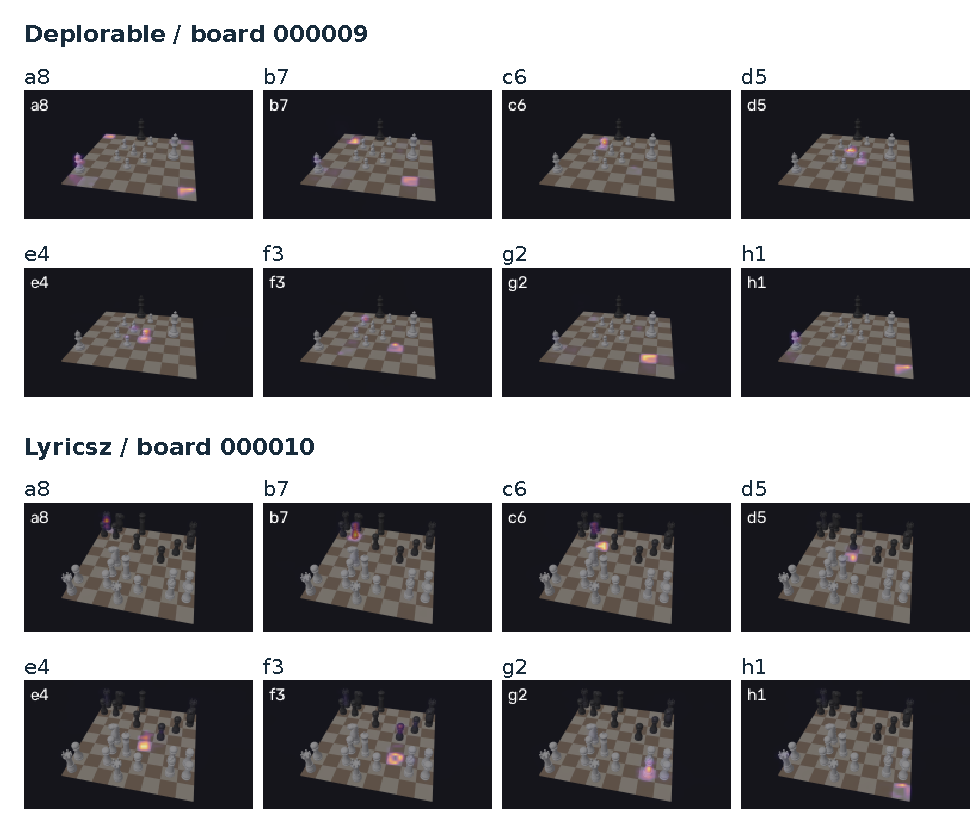
\includegraphics[width=\linewidth]{figures/attention_excerpt.pdf}
  \caption{Fixed, outcome-independent excerpt. Select the first two geometry names
  lexicographically in the frozen attention sample, then the lowest zero-padded
  board ID in each: Deplorable 000009 and Lyricsz 000010. For both boards use the
  same eight diagonal queries, a8, b7, c6, d5, e4, f3, g2 and h1. No prediction,
  correctness, confidence or attention magnitude enters this selection. Tiles are
  unchanged crops of the recorded overlays, normalized per query, not a shared
  saliency scale. The full set has 60 sheets (30 boards, 64 queries, two
  projections). Three sheets ship in the package, in \texttt{figures/attention/}.
  The full set is not released.}
  \label{fig:attention-excerpt}
\end{figure}


\FloatBarrier
\clearpage
\section{Receipt and test index}
\label{app:receipts}

The evidence index carries the digest of each copied file. Digests of the unredacted
originals are not shipped.
Table~\ref{tab:receipts} lists the completion receipts consumed by the generated tables
and figures, and the result summaries behind the Section~\ref{sec:lies} numbers (parity probe,
crop diagnostic, baseline and member scores, identifier-level holdout check, real-board check).
Per-image prediction files for those runs are not part of this package. A completion receipt records the checks stated by its own schema;
it is a checksummed record, not an independent attestation that no unrecorded
experiment occurred. It does not close the separate data, model, or asset
distribution gates.

\begingroup\small
\setlength{\tabcolsep}{4pt}
\begin{longtable}{>{\raggedright\arraybackslash}p{.49\linewidth}>{\raggedright\arraybackslash}p{.44\linewidth}}
\caption{Receipt and result-summary index. Paths and the hash of each copy are in the evidence index.}\label{tab:receipts}\\
\toprule
Receipt filename & % receipt: evidence/index.json; source: evidence/index.json; column definitions
Status / schema \\ % receipt: evidence/index.json; source: evidence/index.json; column definitions
\midrule

\endfirsthead
\toprule
Receipt filename & % receipt: evidence/index.json; source: evidence/index.json; column definitions
Status / schema \\ % receipt: evidence/index.json; source: evidence/index.json; column definitions
\midrule

\endhead
\bottomrule\endfoot
adaptation.complete.json & % receipt: evidence/index.json; source: evidence/index.json; benchmark_v2/adaptation.complete.json
schema\_\allowbreak{}v2\_\allowbreak{}frozen \\ % receipt: evidence/index.json; source: evidence/index.json; benchmark_v2/adaptation.complete.json

benchmark.complete.json & % receipt: evidence/index.json; source: evidence/index.json; benchmark_v2/benchmark.complete.json
schema\_\allowbreak{}v2\_\allowbreak{}frozen \\ % receipt: evidence/index.json; source: evidence/index.json; benchmark_v2/benchmark.complete.json

design.complete.json & % receipt: evidence/index.json; source: evidence/index.json; benchmark_v2/design.complete.json
design\_\allowbreak{}locked\_\allowbreak{}before\_\allowbreak{}rendering \\ % receipt: evidence/index.json; source: evidence/index.json; benchmark_v2/design.complete.json

exclusion\_\allowbreak{}audit.complete.json & % receipt: evidence/index.json; source: evidence/index.json; benchmark_v2/exclusion_audit.complete.json
all\_\allowbreak{}required\_\allowbreak{}sources\_\allowbreak{}audited \\ % receipt: evidence/index.json; source: evidence/index.json; benchmark_v2/exclusion_audit.complete.json

PARITY\_\allowbreak{}CONVENTIONS.complete.json & % receipt: evidence/index.json; source: evidence/index.json; docs/records/PARITY_CONVENTIONS.complete.json
parity-conventions-audit/v1 \\ % receipt: evidence/index.json; source: evidence/index.json; docs/records/PARITY_CONVENTIONS.complete.json

PHUONG\_\allowbreak{}LICENCE\_\allowbreak{}RECOVERY.complete.json & % receipt: evidence/index.json; source: evidence/index.json; docs/records/PHUONG_LICENCE_RECOVERY.complete.json
licence\_\allowbreak{}recovery\_\allowbreak{}complete\_\allowbreak{}version\_\allowbreak{}unresolved \\ % receipt: evidence/index.json; source: evidence/index.json; docs/records/PHUONG_LICENCE_RECOVERY.complete.json

PHUONG\_\allowbreak{}RELEASE\_\allowbreak{}STATUS\_\allowbreak{}2026-09-14.complete.json & % receipt: evidence/index.json; source: evidence/index.json; docs/records/PHUONG_RELEASE_STATUS_2026-09-14.complete.json
operator\_\allowbreak{}decision\_\allowbreak{}applied \\ % receipt: evidence/index.json; source: evidence/index.json; docs/records/PHUONG_RELEASE_STATUS_2026-09-14.complete.json

PHUONG\_\allowbreak{}RELEASE\_\allowbreak{}STATUS\_\allowbreak{}2026-09-15.complete.json & % receipt: evidence/index.json; source: evidence/index.json; docs/records/PHUONG_RELEASE_STATUS_2026-09-15.complete.json
author\_\allowbreak{}notice\_\allowbreak{}bindings\_\allowbreak{}updated \\ % receipt: evidence/index.json; source: evidence/index.json; docs/records/PHUONG_RELEASE_STATUS_2026-09-15.complete.json

PHUONG\_\allowbreak{}RELEASE\_\allowbreak{}STATUS\_\allowbreak{}2026-10-12.complete.json & % receipt: evidence/index.json; source: evidence/index.json; docs/records/PHUONG_RELEASE_STATUS_2026-10-12.complete.json
public\_\allowbreak{}doc\_\allowbreak{}notice\_\allowbreak{}bindings\_\allowbreak{}updated \\ % receipt: evidence/index.json; source: evidence/index.json; docs/records/PHUONG_RELEASE_STATUS_2026-10-12.complete.json

RELEASE\_\allowbreak{}LICENCE\_\allowbreak{}REVIEW.complete.json & % receipt: evidence/index.json; source: evidence/index.json; docs/records/RELEASE_LICENCE_REVIEW.complete.json
licence\_\allowbreak{}review\_\allowbreak{}complete\_\allowbreak{}with\_\allowbreak{}open\_\allowbreak{}release\_\allowbreak{}gates \\ % receipt: evidence/index.json; source: evidence/index.json; docs/records/RELEASE_LICENCE_REVIEW.complete.json

lora\_\allowbreak{}report.complete.json & % receipt: evidence/index.json; source: evidence/index.json; tools/reports/paper/lora_curve_2026-09-10/lora_report.complete.json
lora\_\allowbreak{}curve\_\allowbreak{}report\_\allowbreak{}complete \\ % receipt: evidence/index.json; source: evidence/index.json; tools/reports/paper/lora_curve_2026-09-10/lora_report.complete.json

result\_\allowbreak{}r1.complete.json & % receipt: evidence/index.json; source: evidence/index.json; tools/reports/paper/parity_probe_2026-09-09/result_r1.complete.json
completed\_\allowbreak{}exploratory\_\allowbreak{}probe \\ % receipt: evidence/index.json; source: evidence/index.json; tools/reports/paper/parity_probe_2026-09-09/result_r1.complete.json

precision\_\allowbreak{}results.complete.json & % receipt: evidence/index.json; source: evidence/index.json; tools/reports/paper/residual_shift_2026-09-10/diagnostics/precision_results.complete.json
c3\_\allowbreak{}precision\_\allowbreak{}probe\_\allowbreak{}complete \\ % receipt: evidence/index.json; source: evidence/index.json; tools/reports/paper/residual_shift_2026-09-10/diagnostics/precision_results.complete.json

overall\_\allowbreak{}recovery.complete.json & % receipt: evidence/index.json; source: evidence/index.json; tools/reports/paper/residual_shift_2026-09-10/overall_recovery.complete.json
complete\_\allowbreak{}after\_\allowbreak{}c3\_\allowbreak{}precision\_\allowbreak{}instrumentation\_\allowbreak{}recovery \\ % receipt: evidence/index.json; source: evidence/index.json; tools/reports/paper/residual_shift_2026-09-10/overall_recovery.complete.json

residual\_\allowbreak{}r1.complete.json & % receipt: evidence/index.json; source: evidence/index.json; tools/reports/paper/residual_shift_2026-09-10/r1/residual_r1.complete.json
c3\_\allowbreak{}residual\_\allowbreak{}complete \\ % receipt: evidence/index.json; source: evidence/index.json; tools/reports/paper/residual_shift_2026-09-10/r1/residual_r1.complete.json

timing.complete.json & % receipt: evidence/index.json; source: evidence/index.json; tools/reports/paper/timing_2026-09-10/timing.complete.json
c4\_\allowbreak{}timing\_\allowbreak{}complete \\ % receipt: evidence/index.json; source: evidence/index.json; tools/reports/paper/timing_2026-09-10/timing.complete.json

cq\_\allowbreak{}release.complete.json & % receipt: evidence/index.json; source: evidence/index.json; tools/reports/paper/timing_2026-09-10/timing.runs/cq_release.complete.json
c4\_\allowbreak{}timing\_\allowbreak{}complete \\ % receipt: evidence/index.json; source: evidence/index.json; tools/reports/paper/timing_2026-09-10/timing.runs/cq_release.complete.json

lora\_\allowbreak{}both\_\allowbreak{}n2000\_\allowbreak{}s303.complete.json & % receipt: evidence/index.json; source: evidence/index.json; tools/reports/paper/timing_2026-09-10/timing.runs/lora_both_n2000_s303.complete.json
c4\_\allowbreak{}timing\_\allowbreak{}complete \\ % receipt: evidence/index.json; source: evidence/index.json; tools/reports/paper/timing_2026-09-10/timing.runs/lora_both_n2000_s303.complete.json

lora\_\allowbreak{}both\_\allowbreak{}n2000\_\allowbreak{}s304.complete.json & % receipt: evidence/index.json; source: evidence/index.json; tools/reports/paper/timing_2026-09-10/timing.runs/lora_both_n2000_s304.complete.json
c4\_\allowbreak{}timing\_\allowbreak{}complete \\ % receipt: evidence/index.json; source: evidence/index.json; tools/reports/paper/timing_2026-09-10/timing.runs/lora_both_n2000_s304.complete.json

lora\_\allowbreak{}both\_\allowbreak{}n2000\_\allowbreak{}s305.complete.json & % receipt: evidence/index.json; source: evidence/index.json; tools/reports/paper/timing_2026-09-10/timing.runs/lora_both_n2000_s305.complete.json
c4\_\allowbreak{}timing\_\allowbreak{}complete \\ % receipt: evidence/index.json; source: evidence/index.json; tools/reports/paper/timing_2026-09-10/timing.runs/lora_both_n2000_s305.complete.json

lora\_\allowbreak{}both\_\allowbreak{}n500\_\allowbreak{}s303.complete.json & % receipt: evidence/index.json; source: evidence/index.json; tools/reports/paper/timing_2026-09-10/timing.runs/lora_both_n500_s303.complete.json
c4\_\allowbreak{}timing\_\allowbreak{}complete \\ % receipt: evidence/index.json; source: evidence/index.json; tools/reports/paper/timing_2026-09-10/timing.runs/lora_both_n500_s303.complete.json

lora\_\allowbreak{}both\_\allowbreak{}n8000\_\allowbreak{}s303.complete.json & % receipt: evidence/index.json; source: evidence/index.json; tools/reports/paper/timing_2026-09-10/timing.runs/lora_both_n8000_s303.complete.json
c4\_\allowbreak{}timing\_\allowbreak{}complete \\ % receipt: evidence/index.json; source: evidence/index.json; tools/reports/paper/timing_2026-09-10/timing.runs/lora_both_n8000_s303.complete.json

lora\_\allowbreak{}dark\_\allowbreak{}n2000\_\allowbreak{}s303.complete.json & % receipt: evidence/index.json; source: evidence/index.json; tools/reports/paper/timing_2026-09-10/timing.runs/lora_dark_n2000_s303.complete.json
c4\_\allowbreak{}timing\_\allowbreak{}complete \\ % receipt: evidence/index.json; source: evidence/index.json; tools/reports/paper/timing_2026-09-10/timing.runs/lora_dark_n2000_s303.complete.json

lora\_\allowbreak{}dark\_\allowbreak{}n2000\_\allowbreak{}s304.complete.json & % receipt: evidence/index.json; source: evidence/index.json; tools/reports/paper/timing_2026-09-10/timing.runs/lora_dark_n2000_s304.complete.json
c4\_\allowbreak{}timing\_\allowbreak{}complete \\ % receipt: evidence/index.json; source: evidence/index.json; tools/reports/paper/timing_2026-09-10/timing.runs/lora_dark_n2000_s304.complete.json

lora\_\allowbreak{}dark\_\allowbreak{}n2000\_\allowbreak{}s305.complete.json & % receipt: evidence/index.json; source: evidence/index.json; tools/reports/paper/timing_2026-09-10/timing.runs/lora_dark_n2000_s305.complete.json
c4\_\allowbreak{}timing\_\allowbreak{}complete \\ % receipt: evidence/index.json; source: evidence/index.json; tools/reports/paper/timing_2026-09-10/timing.runs/lora_dark_n2000_s305.complete.json

lora\_\allowbreak{}dark\_\allowbreak{}n500\_\allowbreak{}s303.complete.json & % receipt: evidence/index.json; source: evidence/index.json; tools/reports/paper/timing_2026-09-10/timing.runs/lora_dark_n500_s303.complete.json
c4\_\allowbreak{}timing\_\allowbreak{}complete \\ % receipt: evidence/index.json; source: evidence/index.json; tools/reports/paper/timing_2026-09-10/timing.runs/lora_dark_n500_s303.complete.json

lora\_\allowbreak{}dark\_\allowbreak{}n8000\_\allowbreak{}s303.complete.json & % receipt: evidence/index.json; source: evidence/index.json; tools/reports/paper/timing_2026-09-10/timing.runs/lora_dark_n8000_s303.complete.json
c4\_\allowbreak{}timing\_\allowbreak{}complete \\ % receipt: evidence/index.json; source: evidence/index.json; tools/reports/paper/timing_2026-09-10/timing.runs/lora_dark_n8000_s303.complete.json

private\_\allowbreak{}full.complete.json & % receipt: evidence/index.json; source: evidence/index.json; tools/reports/paper/timing_2026-09-10/timing.runs/private_full.complete.json
c4\_\allowbreak{}timing\_\allowbreak{}complete \\ % receipt: evidence/index.json; source: evidence/index.json; tools/reports/paper/timing_2026-09-10/timing.runs/private_full.complete.json

private\_\allowbreak{}raw.complete.json & % receipt: evidence/index.json; source: evidence/index.json; tools/reports/paper/timing_2026-09-10/timing.runs/private_raw.complete.json
c4\_\allowbreak{}timing\_\allowbreak{}complete \\ % receipt: evidence/index.json; source: evidence/index.json; tools/reports/paper/timing_2026-09-10/timing.runs/private_raw.complete.json

private\_\allowbreak{}warp\_\allowbreak{}high.complete.json & % receipt: evidence/index.json; source: evidence/index.json; tools/reports/paper/timing_2026-09-10/timing.runs/private_warp_high.complete.json
c4\_\allowbreak{}timing\_\allowbreak{}complete \\ % receipt: evidence/index.json; source: evidence/index.json; tools/reports/paper/timing_2026-09-10/timing.runs/private_warp_high.complete.json

private\_\allowbreak{}warp\_\allowbreak{}low.complete.json & % receipt: evidence/index.json; source: evidence/index.json; tools/reports/paper/timing_2026-09-10/timing.runs/private_warp_low.complete.json
c4\_\allowbreak{}timing\_\allowbreak{}complete \\ % receipt: evidence/index.json; source: evidence/index.json; tools/reports/paper/timing_2026-09-10/timing.runs/private_warp_low.complete.json

leak\_\allowbreak{}check\_\allowbreak{}render-host.json & % receipt: evidence/index.json; source: evidence/index.json; data/holdout/leak_check_render-host.json
result summary \\ % receipt: evidence/index.json; source: evidence/index.json; data/holdout/leak_check_render-host.json

cq\_\allowbreak{}baseline\_\allowbreak{}2026-09-08.json & % receipt: evidence/index.json; source: evidence/index.json; tools/reports/paper/cq_baseline_2026-09-08.json
result summary \\ % receipt: evidence/index.json; source: evidence/index.json; tools/reports/paper/cq_baseline_2026-09-08.json

cq\_\allowbreak{}baseline\_\allowbreak{}chesscog\_\allowbreak{}2026-09-08.json & % receipt: evidence/index.json; source: evidence/index.json; tools/reports/paper/cq_baseline_chesscog_2026-09-08.json
result summary \\ % receipt: evidence/index.json; source: evidence/index.json; tools/reports/paper/cq_baseline_chesscog_2026-09-08.json

cq\_\allowbreak{}baseline\_\allowbreak{}cvchess\_\allowbreak{}2026-09-08.json & % receipt: evidence/index.json; source: evidence/index.json; tools/reports/paper/cq_baseline_cvchess_2026-09-08.json
result summary \\ % receipt: evidence/index.json; source: evidence/index.json; tools/reports/paper/cq_baseline_cvchess_2026-09-08.json

crop\_\allowbreak{}diag\_\allowbreak{}2026-09-09.json & % receipt: evidence/index.json; source: evidence/index.json; tools/reports/paper/crop_diag_2026-09-09.json
result summary \\ % receipt: evidence/index.json; source: evidence/index.json; tools/reports/paper/crop_diag_2026-09-09.json

member\_\allowbreak{}cvchess\_\allowbreak{}full.tsv.json & % receipt: evidence/index.json; source: evidence/index.json; tools/reports/paper/member_cvchess_full.tsv.json
result summary \\ % receipt: evidence/index.json; source: evidence/index.json; tools/reports/paper/member_cvchess_full.tsv.json

member\_\allowbreak{}cvchess\_\allowbreak{}raw.tsv.json & % receipt: evidence/index.json; source: evidence/index.json; tools/reports/paper/member_cvchess_raw.tsv.json
result summary \\ % receipt: evidence/index.json; source: evidence/index.json; tools/reports/paper/member_cvchess_raw.tsv.json

member\_\allowbreak{}cvchess\_\allowbreak{}warp\_\allowbreak{}high.tsv.json & % receipt: evidence/index.json; source: evidence/index.json; tools/reports/paper/member_cvchess_warp_high.tsv.json
result summary \\ % receipt: evidence/index.json; source: evidence/index.json; tools/reports/paper/member_cvchess_warp_high.tsv.json

member\_\allowbreak{}cvchess\_\allowbreak{}warp\_\allowbreak{}low.tsv.json & % receipt: evidence/index.json; source: evidence/index.json; tools/reports/paper/member_cvchess_warp_low.tsv.json
result summary \\ % receipt: evidence/index.json; source: evidence/index.json; tools/reports/paper/member_cvchess_warp_low.tsv.json

member\_\allowbreak{}slcctest\_\allowbreak{}full.tsv.json & % receipt: evidence/index.json; source: evidence/index.json; tools/reports/paper/member_slcctest_full.tsv.json
result summary \\ % receipt: evidence/index.json; source: evidence/index.json; tools/reports/paper/member_slcctest_full.tsv.json

member\_\allowbreak{}slcctest\_\allowbreak{}raw.tsv.json & % receipt: evidence/index.json; source: evidence/index.json; tools/reports/paper/member_slcctest_raw.tsv.json
result summary \\ % receipt: evidence/index.json; source: evidence/index.json; tools/reports/paper/member_slcctest_raw.tsv.json

member\_\allowbreak{}slcctest\_\allowbreak{}warp\_\allowbreak{}high.tsv.json & % receipt: evidence/index.json; source: evidence/index.json; tools/reports/paper/member_slcctest_warp_high.tsv.json
result summary \\ % receipt: evidence/index.json; source: evidence/index.json; tools/reports/paper/member_slcctest_warp_high.tsv.json

member\_\allowbreak{}slcctest\_\allowbreak{}warp\_\allowbreak{}low.tsv.json & % receipt: evidence/index.json; source: evidence/index.json; tools/reports/paper/member_slcctest_warp_low.tsv.json
result summary \\ % receipt: evidence/index.json; source: evidence/index.json; tools/reports/paper/member_slcctest_warp_low.tsv.json

analysis.json & % receipt: evidence/index.json; source: evidence/index.json; tools/reports/paper/parity_probe_2026-09-09/analysis.json
result summary \\ % receipt: evidence/index.json; source: evidence/index.json; tools/reports/paper/parity_probe_2026-09-09/analysis.json

score\_\allowbreak{}cq\_\allowbreak{}cpu\_\allowbreak{}20261004.json & % receipt: evidence/index.json; source: evidence/index.json; tools/reports/paper/real_photo_2026-09-11/a1_light_2026-10-04/score_cq_cpu_20261004.json
result summary \\ % receipt: evidence/index.json; source: evidence/index.json; tools/reports/paper/real_photo_2026-09-11/a1_light_2026-10-04/score_cq_cpu_20261004.json

\end{longtable}
\endgroup


\subsection{Validation scope}
The paper build checks the complete cell matrix, deterministic table generation,
per-cell source comments, and rejection of altered evidence or broken historical
hash links. The export regressions separately test token boundaries, paired
original/export hashes, protected scene records, and explicit PDF decoder
failures. Passing these checks does not validate the scientific claims in the
paper text or resolve a distribution licence.

\subsection{Conditional localization diagnostic}
% receipt: evidence/tools/reports/paper/FREEZE_2026-09-09.json
Figure~\ref{fig:corners} retains the earlier detector summary as a separate
measurement from recognition. This figure and the historical pipeline comparison
use hash-pinned aggregate summaries without original run-completion receipts;
copying their hashes does not retrospectively certify the original runs. Error is normalized by the mean projected board
edge, and the figure reports excluded detections beside the elevation bands.
% historical source summary: evidence/tools/reports/paper/FREEZE_2026-09-09.json
\begin{figure}[htbp]
\centering
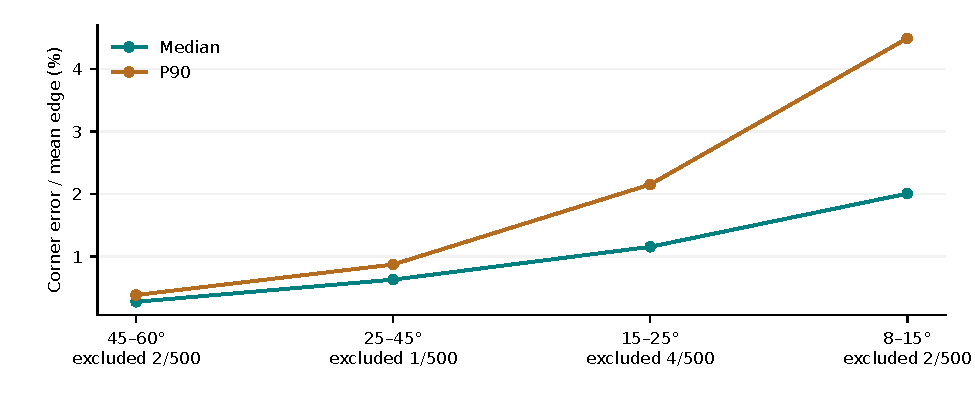
\includegraphics[width=\linewidth]{figures/corner_elevation.pdf}
\caption{Conditional corner error normalized by mean projected board edge. Excluded detections are reported for each elevation band. Historical aggregates are hash-pinned; original run-completion receipts are unavailable.}\label{fig:corners}
\end{figure}



\end{document}
